%%%%%%%%%%%%%%%%%%%%%%%%%%%%%%%%%%%%%%%%%%%%%%%%%%%%%%%%%%%%%%%%%%%%%%%%%%%%%%%
%                                                                             %
% Copyright (C) 2005-2006,2008,2012-2015,2018 Edward d'Auvergne               %
%                                                                             %
% This file is part of the program relax (http://www.nmr-relax.com).          %
%                                                                             %
% This program is free software: you can redistribute it and/or modify        %
% it under the terms of the GNU General Public License as published by        %
% the Free Software Foundation, either version 3 of the License, or           %
% (at your option) any later version.                                         %
%                                                                             %
% This program is distributed in the hope that it will be useful,             %
% but WITHOUT ANY WARRANTY; without even the implied warranty of              %
% MERCHANTABILITY or FITNESS FOR A PARTICULAR PURPOSE.  See the               %
% GNU General Public License for more details.                                %
%                                                                             %
% You should have received a copy of the GNU General Public License           %
% along with this program.  If not, see <http://www.gnu.org/licenses/>.       %
%                                                                             %
%%%%%%%%%%%%%%%%%%%%%%%%%%%%%%%%%%%%%%%%%%%%%%%%%%%%%%%%%%%%%%%%%%%%%%%%%%%%%%%


\documentclass[a4paper, 11pt, twoside, openright]{book}

% Graphics.
\usepackage[dvips]{graphicx}

% Natural Sciences Citations and References.
\usepackage{natbib}

% The index.
\usepackage{imakeidx}

% Good looking tables.
\usepackage{booktabs}
\usepackage{longtable}
\usepackage{tabularx}
\usepackage{rotating}
\usepackage{lscape}
\usepackage[flushleft]{threeparttable}

% Nth.
\usepackage[super]{nth}

% Obliterate those painful LaTeX margins!
\usepackage{vmargin}

% Better screenshot layout.
\raggedbottom

% Better Table of contents (Toc), List of figures (Lof), and List of tables (Lot).
\usepackage{tocloft}

% Hyperlinks.
\usepackage[pdftitle={The relax manual}]{hyperref}
\hypersetup{colorlinks,
            citecolor=blue,%
            filecolor=blue,%
            linkcolor=blue,%
            urlcolor=blue}
\usepackage{breakurl}

% Better maths.
\usepackage{amsmath}
\usepackage{amssymb}
\usepackage{mathdots}
\usepackage{mathrsfs}
\usepackage{arydshln}
\usepackage{bigints}

% Source code and scripts.
\usepackage[procnames]{listings}
\usepackage[svgnames]{xcolor}
\usepackage{textcomp}
\include{script_definition}
\lstset{
    backgroundcolor=\color{white},
    basewidth=0.5em,
    basicstyle=\ttfamily \footnotesize,
    breakatwhitespace=false,
    breaklines=true,
    captionpos=b,
    columns=fixed,
    commentstyle=\color{Blue},
    frame=none,
    keepspaces=true,
    keywordstyle=\bfseries \color{ForestGreen},
    keywordstyle=[2]\bfseries \color{BlueViolet},
    keywordstyle=[3]\bfseries \color{SaddleBrown},
    keywordstyle=[4]\bfseries \color{Blue},
    keywordstyle=[5]\bfseries \color{MidnightBlue},
    language=relax,
    numbers=left,
    numbersep=15pt,
    numberstyle=\tiny \color{DarkOrange},
    procnamestyle=\color{LightSeaGreen},
    showspaces=false,
    showstringspaces=false,
    showtabs=false,
    stepnumber=1,
    stringstyle=\color{FireBrick},
    tabsize=4,
    upquote=true,
}

% Table row formatting.
\usepackage{array}
\newcolumntype{+}{>{\global\let\currentrowstyle\relax}}
\newcolumntype{^}{>{\currentrowstyle}}
\newcommand{\rowstyle}[1]{\gdef\currentrowstyle{#1}%
    #1\ignorespaces
}

% New commands.
\newcommand{\example}[1]{\vspace{-1ex} \sloppy{\footnotesize \texttt{#1}}}
\newcommand{\smallexample}[1]{\vspace{-1ex} \sloppy{\scriptsize \texttt{#1}}}
\newcommand{\keyword}[1]{\textsf{#1}}
\newcommand{\quotecmd}[1]{`\texttt{#1}'}
\newcommand{\uf}[1]{\texttt{#1}}
\newcommand{\prompt}[1]{\texttt{#1}}
\newcommand{\promptstring}[1]{``\texttt{#1}''}
\newcommand{\shortcutkey}[1]{``{\small \textsf{[#1]}}''}
\newcommand{\gui}[1]{``{\small \textsf{#1}}''}
\newcommand{\guibutton}[1]{``{\small \textsf{#1}}''}
\newcommand{\guimenuitemone}[1]{``{\small \textsf{#1}}''}
\newcommand{\guimenuitemtwo}[2]{``{\small \textsf{#1$\to$\linebreak[0]#2}}''}
\newcommand{\guimenuitemthree}[3]{``{\small \textsf{#1$\to$\linebreak[0]#2$\to$\linebreak[0]#3}}''}
\newcommand{\guistring}[1]{``{\small \textsf{#1}}''}
\newcommand{\directory}[1]{\texttt{#1}}
\newcommand{\file}[1]{\texttt{#1}}
\newcommand{\module}[1]{\texttt{#1}}
\newcommand{\ossep}{/\linebreak[0]}
\newcommand{\osus}{\_\linebreak[0]}
\newcommand{\pycode}[1]{{\small \texttt{#1}}}
\newcommand{\pysep}{.\linebreak[0]}
\newcommand{\pystring}[1]{`{\small \texttt{#1}}'}
\newcommand{\pyus}{\_\linebreak[0]}
\newcommand{\software}[1]{\texttt{#1}}
\newcommand{\no}{-}
\newcommand{\yes}{\checkmark}
\newcommand{\ufsep}{.\linebreak[0]}
\newcommand{\ufus}{\_\linebreak[0]}

% New environment.
\newenvironment{exampleenv}{\begin{footnotesize} \begin{ttfamily} \sloppy}{\fussy \end{ttfamily} \end{footnotesize}}
\newenvironment{spacedpara}{\setlength{\parindent}{0pt} \setlength{\parskip}{2ex plus 0.5ex minus 0.2ex}}{}

% Modify the Toc, Lof, and Lot layout.
\setlength{\cftsecnumwidth}{10mm}
\setlength{\cftsubsecnumwidth}{16mm}
\setlength{\cftfignumwidth}{12mm}
\setlength{\cfttabnumwidth}{12mm}

% The frame order symbol (the daeg runic character)
\usepackage{allrunes}

% Maths commands.
\setcounter{MaxMatrixCols}{20}
\DeclareMathOperator{\arccosh}{arccosh}
\newcommand{\Par}{{\scriptscriptstyle \parallel}}
\newcommand{\Per}{{\scriptscriptstyle \perp}}
\newcommand{\Diff}{\mathfrak{D}}
\newcommand{\Ri}{\mathrm{R}_i}
\newcommand{\Rone}{\mathrm{R}_1}
\newcommand{\Ronerho}{\mathrm{R}_{1\rho}}
\newcommand{\Rtwo}{\mathrm{R}_2}
\newcommand{\NOE}{\mathrm{NOE}}
\newcommand{\crossrate}{\sigma_{\scriptscriptstyle \mathrm{NOE}}}
\newcommand{\gH}{\gamma_{\scriptscriptstyle H}}
\newcommand{\gX}{\gamma_{\scriptscriptstyle X}}
\newcommand{\Spaceset}{\mathfrak{K}}
\newcommand{\Univset}{\mathfrak{U}}
\newcommand{\Space}{\mathfrak{S}}
\newcommand{\Diffset}{\mathfrak{D}}
\newcommand{\Diffgeoset}{\mathfrak{G}}
\newcommand{\Difforiset}{\mathfrak{O}}
\newcommand{\Mfset}{\mathfrak{F}}
\newcommand{\Localset}{\mathfrak{T}}
\newcommand{\KL}{\Delta_{\scriptscriptstyle \text{K-L}}}

\newcommand{\aveoffset}{\overline{\Omega}}
\newcommand{\offsetA}{\Omega_{\textrm{A}}}
\newcommand{\offsetB}{\Omega_{\textrm{B}}}
\newcommand{\offsetC}{\Omega_{\textrm{C}}}
\newcommand{\aveomega}{\overline{\omega}}
\newcommand{\dw}{\Delta\omega}
\newcommand{\dwAB}{\Delta\omega_{\textrm{AB}}}
\newcommand{\dwAC}{\Delta\omega_{\textrm{AC}}}
\newcommand{\dwBC}{\Delta\omega_{\textrm{BC}}}
\newcommand{\dwH}{\Delta\omega^{\scriptscriptstyle\mathrm{H}}}
\newcommand{\dwHAB}{\Delta\omega^{\scriptscriptstyle\mathrm{H}}_{\textrm{AB}}}
\newcommand{\dwHAC}{\Delta\omega^{\scriptscriptstyle\mathrm{H}}_{\textrm{AC}}}
\newcommand{\dwHBC}{\Delta\omega^{\scriptscriptstyle\mathrm{H}}_{\textrm{BC}}}
\newcommand{\konetwo}{\textrm{k}_{\textrm{12}}}
\newcommand{\konethree}{\textrm{k}_{\textrm{13}}}
\newcommand{\koneN}{\textrm{k}_{\textrm{1N}}}
\newcommand{\kex}{\textrm{k}_{\textrm{ex}}}
\newcommand{\kexAB}{\textrm{k}_{\textrm{ex}}^{\textrm{AB}}}
\newcommand{\kexAC}{\textrm{k}_{\textrm{ex}}^{\textrm{AC}}}
\newcommand{\kexBC}{\textrm{k}_{\textrm{ex}}^{\textrm{BC}}}
\newcommand{\kA}{\textrm{k}_{\textrm{A}}}
\newcommand{\kB}{\textrm{k}_{\textrm{B}}}
\newcommand{\kC}{\textrm{k}_{\textrm{C}}}
\newcommand{\kAB}{\textrm{k}_{\textrm{AB}}}
\newcommand{\kBA}{\textrm{k}_{\textrm{BA}}}
\newcommand{\kAC}{\textrm{k}_{\textrm{AC}}}
\newcommand{\kCA}{\textrm{k}_{\textrm{CA}}}
\newcommand{\kBC}{\textrm{k}_{\textrm{BC}}}
\newcommand{\kCB}{\textrm{k}_{\textrm{CB}}}
\newcommand{\ncyc}{N_{\textrm{cyc}}}
\newcommand{\nucpmg}{\nu_{\textrm{CPMG}}}
\newcommand{\omegaA}{\omega_{\textrm{A}}}
\newcommand{\omegaB}{\omega_{\textrm{B}}}
\newcommand{\omegaC}{\omega_{\textrm{C}}}
\newcommand{\omegae}{\omega_{\textrm{e}}}
\newcommand{\omegaHA}{\omega^{\scriptscriptstyle\mathrm{H}}_{\textrm{A}}}
\newcommand{\omegaHB}{\omega^{\scriptscriptstyle\mathrm{H}}_{\textrm{B}}}
\newcommand{\omegaHC}{\omega^{\scriptscriptstyle\mathrm{H}}_{\textrm{C}}}
\newcommand{\omegaone}{\omega_1}
\newcommand{\omegarf}{\omega_{\textrm{rf}}}
\newcommand{\pone}{p_{\textrm{1}}}
\newcommand{\ptwo}{p_{\textrm{2}}}
\newcommand{\pthree}{p_{\textrm{3}}}
\newcommand{\pA}{p_{\textrm{A}}}
\newcommand{\pB}{p_{\textrm{B}}}
\newcommand{\pC}{p_{\textrm{C}}}
\newcommand{\pN}{p_{\textrm{N}}}
\newcommand{\Phiex}{\Phi_{\textrm{ex}}}
\newcommand{\PhiexB}{\Phi_{\textrm{ex,B}}}
\newcommand{\PhiexC}{\Phi_{\textrm{ex,C}}}
\newcommand{\Phiexi}{\Phi_{\textrm{ex,i}}}
\newcommand{\Rex}{\mathrm{R}_{\textrm{ex}}}
\newcommand{\RoneA}{\mathrm{R}_{\textrm{1A}}}
\newcommand{\RoneB}{\mathrm{R}_{\textrm{1B}}}
\newcommand{\RoneC}{\mathrm{R}_{\textrm{1C}}}
\newcommand{\Ronerhoprime}{\mathrm{R}_{1\rho}'}
\newcommand{\RonerhoprimeA}{\mathrm{R}_{1\rho A}'}
\newcommand{\RonerhoprimeB}{\mathrm{R}_{1\rho B}'}
\newcommand{\RonerhoprimeC}{\mathrm{R}_{1\rho C}'}
\newcommand{\Rtwoeff}{\mathrm{R}_{\textrm{2eff}}}
\newcommand{\RtwoeffCR}{\mathrm{R}_{\textrm{2eff}}^{\textrm{CR72}}}
\newcommand{\Rtwozero}{\mathrm{R}_2^0}
\newcommand{\RtwozeroA}{\mathrm{R}_{\mathrm{2A}}^0}
\newcommand{\RtwozeroB}{\mathrm{R}_{\mathrm{2B}}^0}
\newcommand{\RtwozeroC}{\mathrm{R}_{\mathrm{2C}}^0}
\newcommand{\RtwozeroMQ}{\mathrm{R}_{\mathrm{2,MQ}}^0}
\newcommand{\RtwoDQA}{\mathrm{R}_{\mathrm{2,DQ}}^{\mathrm{A}}}
\newcommand{\RtwoDQB}{\mathrm{R}_{\mathrm{2,DQ}}^{\mathrm{B}}}
\newcommand{\RtwoDQC}{\mathrm{R}_{\mathrm{2,DQ}}^{\mathrm{C}}}
\newcommand{\RtwoZQA}{\mathrm{R}_{\mathrm{2,ZQ}}^{\mathrm{A}}}
\newcommand{\RtwoZQB}{\mathrm{R}_{\mathrm{2,ZQ}}^{\mathrm{B}}}
\newcommand{\RtwoZQC}{\mathrm{R}_{\mathrm{2,ZQ}}^{\mathrm{C}}}
\newcommand{\tex}{\tau_{\textrm{ex}}}
\newcommand{\taucpmg}{\tau_{\textrm{CPMG}}}
\newcommand{\Trelax}{T_{\textrm{relax}}}

% Maths commands - frame order specific.
\DeclareMathOperator{\pec}{pec}
\DeclareMathOperator{\sinc}{sinc}
\newcommand{\Eigenset}{\mathfrak{E}}
\newcommand{\Eigensetabc}{\mathfrak{E}_{\alpha\beta\gamma}}
\newcommand{\Eigenseta}{\mathfrak{E}^\alpha_{\textrm{ax}}}
\newcommand{\Eigensetafull}{\left\{ \frameaxa \right\}}
\newcommand{\Eigensetax}{\mathfrak{E}_{\textrm{ax}}}
\newcommand{\Eigensetaxfull}{\left\{ \framet, \framep \right\}}
\newcommand{\Eigensetfull}{\left\{ \framea, \frameb, \frameg \right\}}
\newcommand{\FO}{\textarc{d}}
\newcommand{\FOn}{\textarc{d}^{(n)}}
\newcommand{\FOnp}{\textarc{d}^{(n)'}}
\newcommand{\FOone}{\textarc{d}^{(1)}}
\newcommand{\FOonep}{\textarc{d}^{(1)'}}
\newcommand{\FOtwo}{\textarc{d}^{(2)}}
\newcommand{\FOtwop}{\textarc{d}^{(2)'}}
\newcommand{\FOthree}{\textarc{d}^{(3)}}
\newcommand{\FOfour}{\textarc{d}^{(4)}}
\newcommand{\Modelset}{\mathfrak{M}}
\newcommand{\Orderset}{\mathfrak{S}}
\newcommand{\Orientset}{\mathfrak{O}}
\newcommand{\Pivotsetone}{\mathfrak{p}_1}
\newcommand{\Pivotsetonefull}{\left\{ \pivotx, \pivoty, \pivotz \right\}}
\newcommand{\Pivotsettwo}{\mathfrak{p}_2}
\newcommand{\Posset}{\mathfrak{P}}
\newcommand{\Possetfull}{\left\{ \aveposx, \aveposy, \aveposz, \aveposa, \aveposb, \aveposg \right\}}
\newcommand{\Possetred}{\mathfrak{P}'}
\newcommand{\Translateset}{\mathfrak{T}}
\newcommand{\aveposa}{P_\alpha}
\newcommand{\aveposb}{P_\beta}
\newcommand{\aveposg}{P_\gamma}
\newcommand{\aveposi}{P_i}
\newcommand{\aveposx}{P_x}
\newcommand{\aveposy}{P_y}
\newcommand{\aveposz}{P_z}
\newcommand{\conetheta}{\theta}
\newcommand{\conethetamax}{\theta_{\textrm{max}}}
\newcommand{\conethetax}{\theta_x}
\newcommand{\conethetay}{\theta_y}
\newcommand{\conesmax}{\sigma_{\textrm{max}}}
\newcommand{\conesmaxi}{\sigma_{\textrm{max,i}}}
\newcommand{\conesmaxone}{\sigma_{\textrm{max,1}}}
\newcommand{\conesmaxtwo}{\sigma_{\textrm{max,2}}}
\newcommand{\diff}{\,\mathrm{d}}
\newcommand{\framea}{E_\alpha}
\newcommand{\frameaxa}{E_\alpha^{\textrm{ax}}}
\newcommand{\frameb}{E_\beta}
\newcommand{\frameg}{E_\gamma}
\newcommand{\framei}{E_i}
\newcommand{\framep}{E_\phi}
\newcommand{\framet}{E_\theta}
\newcommand{\half}{\tfrac{1}{2}}
\newcommand{\quart}{\tfrac{1}{4}}
\newcommand{\permA}{^{\textrm{A}}}
\newcommand{\permB}{^{\textrm{B}}}
\newcommand{\pivotdisp}{p_d}
\newcommand{\pivoti}{p_i}
\newcommand{\pivotx}{p_x}
\newcommand{\pivoty}{p_y}
\newcommand{\pivotz}{p_z}
\newcommand{\sincsigma}{\textrm{s}_\sigma}
\newcommand{\sinctwosigma}{\textrm{s}_{2\sigma}}
\newcommand{\raxhat}{\hat{r}_{ax}}
\newcommand{\rCoMpivhat}{\hat{r}_{\textrm{CoM}-\Pivotsetone}}
\newcommand{\tmax}{t_{\textrm{max}}}
\newcommand{\vectr}{r}
\newcommand{\unitvectr}{\hat{r}}

% Natbib Citation format.
\bibpunct{(}{)}{;}{a}{,}{,}

% Inline citations.
\usepackage{bibentry}
\nobibliography*

% Allow the maths blocks to be broken!!!
\allowdisplaybreaks[1]

% Set the graphics path to the parent relax directory.
\graphicspath{{../../}}

% latex2html stuff.
\usepackage{html}
\htmladdtonavigation{\htmladdnormallink{\htmladdimg{http://www.nmr-relax.com/images/pdf_icon_nav.png}}{https://sourceforge.net/projects/nmr-relax/files/manual/relax.pdf/download}}
\htmladdtonavigation{\htmladdnormallink{\htmladdimg{http://www.nmr-relax.com/images/relax_logo_nav.png}}{http://www.nmr-relax.com}}
\begin{htmlonly}
  % Make hyperrefs work in latex2html.
  \def\url#1{\htmladdnormallink{#1}{#1}}
  \def\href#1#2{\htmladdnormallink{#2}{#1}}

  % Support for \bibentry{}.
  \def\bibentry#1{\citet{#1}}

  % Kill the rotate environment that latex2html cannot handle.
  \renewenvironment{rotate}[1]{}

  % Redefine some commands to be prettier in HTML.
  \newcommand{\no}{-}
  \newcommand{\yes}{\begin{rawhtml}&#x2713;\end{rawhtml}}

  \newcommand{\FO}{\textrm{Daeg}}
  \newcommand{\FOn}{\textrm{Daeg}^{(n)}}
  \newcommand{\FOnp}{\textrm{Daeg}^{(n)'}}
  \newcommand{\FOone}{\textrm{Daeg}^{(1)}}
  \newcommand{\FOonep}{\textrm{Daeg}^{(1)'}}
  \newcommand{\FOtwo}{\textrm{Daeg}^{(2)}}
  \newcommand{\FOtwop}{\textrm{Daeg}^{(2)'}}
  \newcommand{\FOthree}{\textrm{Daeg}^{(3)}}
  \newcommand{\FOfour}{\textrm{Daeg}^{(4)}}
\end{htmlonly}

% Make the index.
\makeindex


% Start the document.
%%%%%%%%%%%%%%%%%%%%%

\begin{document}

% Include the hyphenation rules.
%%%%%%%%%%%%%%%%%%%%%%%%%%%%%%%%%%%%%%%%%%%%%%%%%%%%%%%%%%%%%%%%%%%%%%%%%%%%%%%
%                                                                             %
% Copyright (C) 2013,2017 Edward d'Auvergne                                   %
%                                                                             %
% This file is part of the program relax (http://www.nmr-relax.com).          %
%                                                                             %
% This program is free software: you can redistribute it and/or modify        %
% it under the terms of the GNU General Public License as published by        %
% the Free Software Foundation, either version 3 of the License, or           %
% (at your option) any later version.                                         %
%                                                                             %
% This program is distributed in the hope that it will be useful,             %
% but WITHOUT ANY WARRANTY; without even the implied warranty of              %
% MERCHANTABILITY or FITNESS FOR A PARTICULAR PURPOSE.  See the               %
% GNU General Public License for more details.                                %
%                                                                             %
% You should have received a copy of the GNU General Public License           %
% along with this program.  If not, see <http://www.gnu.org/licenses/>.       %
%                                                                             %
%%%%%%%%%%%%%%%%%%%%%%%%%%%%%%%%%%%%%%%%%%%%%%%%%%%%%%%%%%%%%%%%%%%%%%%%%%%%%%%


\hyphenation{an-iso-tro-pic}

\hyphenation{Da-sh-a}

\hyphenation{qu-ad-ra-t-ic}

\hyphenation{in-equ-al-i-t-ies}
\hyphenation{in-equ-al-i-ty}
\hyphenation{iso-trop-ic}

\hyphenation{mol-e-c-ule}

\hyphenation{sph-er-oid}



\frontmatter


% Title page.
%%%%%%%%%%%%%

\begin{titlepage}
\begin{center}

% Vertical centering.
\vspace*{\stretch{2}}

% Title.
{\Huge \textbf{relax}}
\vspace{\stretch{1}}

% relax version number.
{\LARGE \textbf{Version 1.2.12
}}
\vspace{\stretch{1}}

\centerline{
  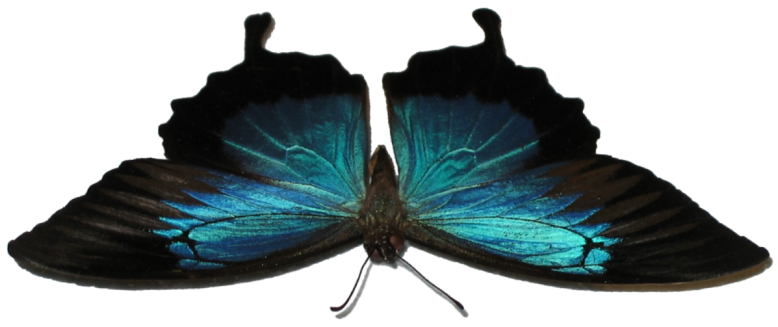
\includegraphics[
    width=\textwidth,
    bb=14 14 793 342
  ]
  {images/ulysses}
}
\vspace{\stretch{2}}

% Subtitle.
{\huge \textbf{Molecular dynamics by}}
\vspace{\stretch{0.5}}

{\huge \textbf{NMR data analysis}}
\vspace{\stretch{1}}

% Date.
{\large \today}
\vspace*{\stretch{2}}

\end{center}

% Blank page with the copyright notice.
\clearpage
\thispagestyle{empty}

\mbox{}

\vspace*{\fill}

\input{copyright}

\end{titlepage}


% Table of Contents.
%%%%%%%%%%%%%%%%%%%%

\tableofcontents


% List of Figures.
%%%%%%%%%%%%%%%%%%

\newpage
\listoffigures


% List of Tables.
%%%%%%%%%%%%%%%%%

\newpage
\listoftables


% Abbreviations.
%%%%%%%%%%%%%%%%

\chapter*{Abbreviations}

\begin{description}
  \item[AIC:]  Akaike's Information Criteria (model selection method)
  \item[AICc:]  small sample size corrected AIC (model selection method)
  \item[API:]  application programming interface
  \item[ANOVA:]  analysis of variance (field of statistics)
  \item[BC:]  back calculation
  \item[BIC:]  Bayesian Information Criteria (model selection method)
  \item[BFGS:]  Broyden-Fletcher-Goldfarb-Shanno (optimisation method)
  \item[$C(\tau)$:]  correlation function
  \item[$\chi^2$:]  chi-squared function
  \item[CG:]  conjugate gradient (optimisation)
  \item[CPMG:]  the Carr-Purcell-Meiboom-Gill pulse sequence
  \item[CR72:]  the \citet{CarverRichards72} relaxation dispersion model
  \item[CSA:]  chemical shift anisotropy
  \item[CV:]  cross validation
  \item[CVS:]  Concurrent Versions System (free software version control system)
  \item[$\Diff$:]  the set of diffusion tensor parameters
  \item[$\Diff_\Par$:]  the eigenvalue of the spheroid diffusion tensor corresponding to the unique axis of the tensor
  \item[$\Diff_\Per$:]  the eigenvalue of the spheroid diffusion tensor corresponding to the two axes perpendicular to the unique axis
  \item[$\Diff_a$:]  the anisotropic component of the Brownian rotational diffusion tensor
  \item[$\Diff_{iso}$:]  the isotropic component of the Brownian rotational diffusion tensor
  \item[$\Diff_r$:]  the rhombic component of the Brownian rotational diffusion tensor
  \item[$\Diff_{ratio}$:]  the ratio of $\Diff_\Par$ to $\Diff_\Per$
  \item[$\Diff_x$:]  the eigenvalue of the Brownian rotational diffusion tensor in which the corresponding eigenvector defines the x-axis of the tensor
  \item[$\Diff_y$:]  the eigenvalue of the Brownian rotational diffusion tensor in which the corresponding eigenvector defines the y-axis of the tensor
  \item[$\Diff_z$:]  the eigenvalue of the Brownian rotational diffusion tensor in which the corresponding eigenvector defines the z-axis of the tensor
  \item[DPL94:]  the \citet{Davis94} relaxation dispersion model
  \item[DQ:]  double quantum
  \item[$\epsilon_i$:]  elimination value
  \item[FSF:]  Free Software Foundation
  \item[GNU:]  GNU's Not Unix!
  \item[GPG:]  GNU Privacy Guard (software)
  \item[GPL:]  GNU general public licence
  \item[GUI:]  graphical user interface
  \item[ID string:]  identification string
  \item[IT99:]  the \citet{IshimaTorchia99} relaxation dispersion model
  \item[$J(\omega)$:]  spectral density function
  \item[LM63:]  the \citet{LuzMeiboom63} relaxation dispersion model
  \item[M61:]  the \citet{Meiboom61} relaxation dispersion model
  \item[MC:]  Monte Carlo (simulations)
  \item[MD:]  molecular dynamics (simulations)
  \item[MMQ:]  proton-heteronuclear SQ, ZQ, DQ, and MQ data (multi-multiple quantum)
  \item[MP05:]  the \citet{MiloushevPalmer05} relaxation dispersion model
  \item[MPI:]  message passing interface
  \item[MQ:]  multiple quantum
  \item[NMR:]  if you do not know this one, do not read further
  \item[NNTP:]  network news transfer protocol
  \item[NOE:]  nuclear Overhauser effect
  \item[NS:]  numeric solution
  \item[ORD:]  optical rotatory dispersion
  \item[OS:]  operating system
  \item[PCS:]  pseudocontact shift
  \item[PDB:]  Protein Data Bank
  \item[pdf:]  probability distribution function
  \item[PRE:]  paramagnetic relaxation enhancement
  \item[$r$:]  bond length
  \item[$\Rone$:]  spin-lattice relaxation rate
  \item[$\Rtwo$:]  spin-spin relaxation rate
  \item[$R_{ex}$:]  chemical exchange relaxation rate
  \item[RDC:]  residual dipolar coupling
  \item[RMSD:]  root-mean-square deviation
  \item[ROE:]  rotating-frame Overhauser effect
  \item[RSDM:]  reduced spectral density mapping
  \item[RSS:]  rich site summary (web feed format)
  \item[$S^2$, $S^2_f$, and $S^2_s$:]  model-free generalised order parameters
  \item[SVN:]  Apache Subversion (free software version control system)
  \item[$\tau_e$, $\tau_f$, and $\tau_s$:]  model-free effective internal correlation times
  \item[$\tau_m$:]  global rotational correlation time
  \item[TP02:]  the \citet{TrottPalmer02} relaxation dispersion model
  \item[TAP03:]  the \citet{Trott03} relaxation dispersion model
  \item[TSMFK01:]  the \citet{Tollinger01} relaxation dispersion model
  \item[UI:]  user interface
  \item[XML:]  extensible markup language
  \item[ZQ:]  zero quantum
\end{description}

% Equation numbering fix for latex2html. 
\begin{htmlonly}
\addtocounter{chapter}{-1}
\end{htmlonly}


% Citations.
%%%%%%%%%%%%

\begin{spacedpara}
\tolerance=1000
% Citations.
%%%%%%%%%%%%

\chapter{Preface - citing relax} \label{ch: citations}

The relax project is a large collection of work created by diverse authors.
It is a community driven project created by NMR spectroscopists which supports a broad range of dynamics analyses.
Care must be taken to properly cite the parts of relax that you use so that the correct authors receive the citations and credit they deserve.
The following is a breakdown of all of the citations relating to relax, including the basic citations for the various analysis types.



% The software relax.
%%%%%%%%%%%%%%%%%%%%%

\section*{The software relax}


% relax.
%~~~~~~~

\subsection*{relax references}

The primary citations for relax are:

\begin{itemize}
\item \bibentry{dAuvergneGooley08a}
\item \bibentry{dAuvergneGooley08b}
\end{itemize}


% Graphical user interface.
%~~~~~~~~~~~~~~~~~~~~~~~~~~

\subsection*{Graphical user interface reference}

The primary citation for the GUI is:

\begin{itemize}
\item \bibentry{Bieri11}
\end{itemize}


% The multi-processor.
%~~~~~~~~~~~~~~~~~~~~~

\subsection*{The multi-processor reference}

Although not published, if the multi-processor framework is used to run relax on multi-core systems, grids, or clusters, then please acknowledge the author of that code -- Gary Thompson.



% Specific analyses.
%%%%%%%%%%%%%%%%%%%%

\section*{Specific analyses}

The following subsections list the citations for the individual analysis specific parts of relax.


% Model-free analysis.
%~~~~~~~~~~~~~~~~~~~~~

\subsection*{Model-free analysis references}

The base citations for model-free theory are:

\begin{itemize}
\item \bibentry{LipariSzabo82a}
\item \bibentry{LipariSzabo82b}
\item \bibentry{Clore90a}
\end{itemize}

If the automated analysis of the \file{dauvergne\osus{}protocol.py} sample script or the GUI model-free analysis which uses the same protocol has been used, then the following citations are all implicit:

\begin{itemize}
\item \bibentry{dAuvergneGooley03}
\item \bibentry{dAuvergneGooley06}
\item \bibentry{dAuvergneGooley07}
\item \bibentry{dAuvergneGooley08a}
\item \bibentry{dAuvergneGooley08b}
\end{itemize}

Otherwise, if model-free analysis is used in relax but not via the inbuilt automated protocol, the first reference is for model selection, the second is for eliminating failed model-free models, and the forth is for the optimisation improvements (the third and fifth are for the automated protocol).  All of the model-free implementation details of relax are covered by the PhD thesis (available as a PDF or as a printed version on Amazon.com) of:

\begin{itemize}
\item \bibentry{dAuvergne06}
\end{itemize}

The reference for the hybridisation of different global diffusion models to analyse the residual inter-domain dynamics -- a not very well documented feature of relax -- is:

\begin{itemize}
\item \bibentry{Horne07}
\end{itemize}

If the software Modelfree4 or Dasha are used as replacement optimisation engines from within relax, the citations for Modelfree4 are:

\begin{itemize}
\item \bibentry{Palmer91}
\item \bibentry{Mandel95}
\end{itemize}

and for Dasha:

\begin{itemize}
\item \bibentry{Orekhov95a}
\end{itemize}


% Consistency testing analysis.
%~~~~~~~~~~~~~~~~~~~~~~~~~~~~~~

\subsection*{Consistency testing analysis references}

The base citations for the consistency testing of NMR relaxation is:

\begin{itemize}
\item \bibentry{Fushman99}
\item \bibentry{Farrow95}
\item \bibentry{Fushman98}
\end{itemize}

The first is the main citation, whereas the next are the individual tests.  The citation for the consistency testing of NMR relaxation as implemented in relax is:

\begin{itemize}
\item \bibentry{MorinGagne09a}
\end{itemize}


% N-state model analysis.
%~~~~~~~~~~~~~~~~~~~~~~~~

\subsection*{N-state model analysis references}

Some citations demonstrating as well as presenting the use of the N-state model for diverse analyses types are:

\begin{itemize}
\item \bibentry{Sun11}
\item \bibentry{Erdelyi11}
\end{itemize}


% Reduced spectral density mapping.
%~~~~~~~~~~~~~~~~~~~~~~~~~~~~~~~~~~

\subsection*{Reduced spectral density mapping references}

The base citations for reduced spectral density mapping are:

\begin{itemize}
\item \bibentry{Farrow95}
\item \bibentry{Lefevre96}
\end{itemize}


% Relaxation dispersion.
%~~~~~~~~~~~~~~~~~~~~~~~

\subsection*{Relaxation dispersion references}

For the base citations for relaxation dispersion, please see chapter~\ref{ch: relax-disp} on page~\pageref{ch: relax-disp} for a listing of the individual models.  The main citation is:

\begin{itemize}
\item \bibentry{Morin14}
\end{itemize}



% Generic parts of relax.
%%%%%%%%%%%%%%%%%%%%%%%%%

\section*{Generic parts of relax}

The following subsections will list the citations for the parts of relax independent of the specific analyses.


% Model selection.
%~~~~~~~~~~~~~~~~~

\subsection*{Model selection references}

The citation for the model selection component of relax is:

\begin{itemize}
\item \bibentry{dAuvergneGooley03}
\end{itemize}

The base citations for the specific model selection techniques of AIC, AICc, and BIC are respectively:

\begin{itemize}
\item \bibentry{Akaike73}
\item \bibentry{HurvichTsai89}
\item \bibentry{Schwarz78}
\end{itemize}



% Other citations.
%%%%%%%%%%%%%%%%%%

\section*{Other citations}

If you believe that other citations should be included in this chapter, please contact the relax users mailing list (relax-users at gna.org\index{mailing list!relax-users}).

\end{spacedpara}


%%%%%%%%%%%%%%
% Main text. %
%%%%%%%%%%%%%%

\mainmatter
\begin{spacedpara}


% Layout of the document.
%%%%%%%%%%%%%%%%%%%%%%%%%

\part{The basics}
% Introduction chapter.
%%%%%%%%%%%%%%%%%%%%%%%

\chapter{Introduction}

The program relax is designed for the study of molecular dynamics through the analysis of experimental NMR data. Organic molecules, proteins, RNA, DNA, sugars, and other biomolecules are all supported. It was originally written for the model-free analysis of protein dynamics, though its scope has been significantly expanded.  It is a community driven project created by NMR spectroscopists for NMR spectroscopists.  It supports many analysis types including:

\begin{description}
\item[Model-free analysis] - the Lipari and Szabo model-free analysis of NMR relaxation data
\item[$\Rone$ and $\Rtwo$] - the exponential curve fitting for the calculation of the R$_x$ NMR relaxation rates.
\item[NOE] - the calculation of the steady-state NOE NMR relaxation data.
\item[Data consistency] - the consistency testing of multiple field NMR relaxation data.
\item[RSDM] - Reduced Spectral Density Mapping.
\item[Frame order and N-state model] - study of domain motions via the N-state model and frame order dynamics theories using anisotropic NMR parameters such as RDCs and PCSs.
\item[Stereochemistry] - investigations of absolute stereochemistry of flexible molecules.
\end{description}

The aim of relax is to provide a seamless and extremely flexible environment able to accept input in any format produced by other NMR software, able to faultlessly create input files, control, and read output from various programs including Modelfree and Dasha, output results in many formats, and visualise the data by controlling programs such as Grace\index{software!Grace|textbf}, OpenDX\index{software!OpenDX|textbf}, MOLMOL\index{software!MOLMOL|textbf}, and PyMOL\index{software!PyMOL|textbf}.  All data analysis tools from optimisation to model selection to Monte Carlo simulations are inbuilt into relax. Therefore the use of additional programs is optional.

The flexibility of relax arises from the choice of relax's scripting capabilities, its Python\index{Python|textbf} prompt interface, or its graphical user interface (GUI)\index{GUI|textbf}.  Extremely complex scripts can be created from simple building blocks to fully automate data analysis.  A number of sample scripts have been provided to help understand script construction. In addition, any of Python's powerful features or functions can be incorporated as the script is executed as an arbitrary Python source file within relax's environment.  The modules of relax can also used as a vast library of dynamics related functions by your own software.

relax is free software (free as in freedom) which is licenced under the GNU General Public Licence (GPL)\index{GPL|textbf}. You are free to copy, modify, or redistribute relax under the terms of the GPL. 


% Program features.
%%%%%%%%%%%%%%%%%%%

\section{Program features}


% Literature.
%~~~~~~~~~~~~

\subsection{Literature}

The primary references for the program relax are \citet{dAuvergneGooley08a} and \citet{dAuvergneGooley08b}.  To properly cite the various parts of relax used in your analysis, please see Chapter~\ref{ch: citations} on page~\pageref{ch: citations}.


% Supported NMR theories.
%~~~~~~~~~~~~~~~~~~~~~~~~

\subsection{Supported NMR theories}

The following relaxation data analysis techniques are currently supported by relax:

\begin{itemize}
\item Model-free analysis (\citet{LipariSzabo82a, LipariSzabo82b, Clore90a} and the specific implementation of \citet{dAuvergneGooley03,dAuvergneGooley06,dAuvergneGooley07,dAuvergneGooley08a,dAuvergneGooley08b}).  This includes the hybridisation of global diffusion models to study residual domain dynamics \citep{Horne07}.
\item Reduced spectral density mapping \citep{Farrow95, Lefevre96}\index{reduced spectral density mapping}.
\item Consistency testing -- the validation of multiple field NMR relaxation data \citep{MorinGagne09}.
\item Exponential curve fitting (to find the $\Rone$ and $\Rtwo$ relaxation rates)\index{exponential curve fitting}.
\item Steady-state NOE calculation\index{NOE}.
\item Determination of absolute stereochemistry of flexible molecules via the N-state model using isotropic and anisotropic NMR parameters such as NOE, ROE, and RDC combined with MD simulation or simulated annealing, and ORD \citep{Sun11}.
\item The N-state model for investigating domain motions.
\item The frame order theory.
\item Conformational analysis of paramagnetically tagged molecules via the N-state model \citep{Erdelyi11}.
\item Analysis and comparison of ensembles of structures using RDCs, PCSs, NOEs, etc. (the N-state model of dynamics).
\end{itemize}


% The future.
\subsubsection{The future}

At some time in the future the following techniques are planned to be implemented within relax:

\begin{itemize}
\item Relaxation dispersion\index{relaxation dispersion}.
\item All other dynamics analyses.
\end{itemize}

Because relax is free software, if you would like to contribute addition features, functions, or modules which you have written for your own publications for the benefit of the field, almost anything relating to molecular dynamics may be accepted.  Please see the Open Source chapter on page~\pageref{ch: open source} for more details.



% Data analysis tools.
%~~~~~~~~~~~~~~~~~~~~~

\subsection{Data analysis tools}

The following tools are implemented as modular components to be used by any data analysis technique:

\begin{itemize}
\item Numerous high-precision optimisation algorithms\index{minisation}.
\item Model selection \citep{dAuvergneGooley03, Chen04}\index{model selection}:
    \begin{itemize}
    \item Akaike's Information Criteria (AIC)\index{model selection!AIC}.
    \item Small sample size corrected AIC (AICc)\index{model selection!AICc}.
    \item Bayesian or Schwarz Information Criteria (BIC)\index{model selection!BIC}.
    \item Bootstrap model selection\index{model selection!bootstrap}.
    \item Single-item-out cross-validation (CV)\index{model selection!cross-validation}.
    \item Hypothesis testing ANOVA model selection (only the model-free specific technique of \citet{Mandel95} is supported)\index{model selection!hypothesis testing}\index{model selection!ANOVA}.
    \end{itemize}
\item Monte Carlo simulations (error analysis for all data analysis techniques)\index{Monte Carlo simulation}.
\item Model elimination -- the removal of failed models prior to model selection \citep{dAuvergneGooley06}\index{model elimination}.
\end{itemize}


% Data visualisation.
%~~~~~~~~~~~~~~~~~~~~

\subsection{Data visualisation}

The results of an analysis, or any data input into relax, can be visualised using a number of programs:

\begin{description}
\item[MOLMOL] 1D data can be mapped onto a structure either by the creation of MOLMOL macros or by direct control of the program\index{software!MOLMOL}.
\item[PyMOL] 3D objects such as the diffusion tensor representation can be displayed with the structure\index{software!PyMOL}.
\item[Grace] any 2D data can be plotted\index{software!Grace}.
\item[OpenDX] The chi-squared space of models with three parameters can be mapped and 3D images of the space produced\index{software!OpenDX}.
\end{description}


% Interfacing with other programs.
%~~~~~~~~~~~~~~~~~~~~~~~~~~~~~~~~~

\subsection{Interfacing with other programs}

relax can create the input files, execute in-line, and then read the output of the following programs. These programs can be used as optimisation engines replacing the minimisation algorithms built into relax:

\begin{itemize}
\item Dasha (model-free analysis)\index{software!Dasha}.
\item Modelfree (model-free analysis)\index{software!Modelfree}.
\end{itemize}


% The user interfaces (UI).
%~~~~~~~~~~~~~~~~~~~~~~~~~~

\subsection{The user interfaces (UI)}

relax can be used through the following UIs:

\begin{description}
\item[The prompt] this is the primary interface of relax. Rather than reinventing a new command language, relax's interface is the powerful Python prompt. This gives the power user full access to a proven programming language.  See Figure~\ref{fig: relax prompt} for a screenshot.
\item[Scripting] this provides a more powerful and flexible framework for controlling the program. The script will be executed as Python code enabling advanced programming for automating data analysis. All the features available within the prompt environment are accessible to the script.  See Figure~\ref{fig: relax script} for a screenshot.
\item[GUI] the graphical user interface provides a sub-set of relax's features - the automatic R$_1$ and R$_2$ relaxation rate curve-fitting, the NOE calculations, and the automatic model-free analysis provided by the \texttt{dauvergne\_protocol} module \citep{dAuvergneGooley08b}.  See Figure~\ref{fig: GUI screenshot - start} for a screenshot.
\end{description}



% The relax HOWTO.
%%%%%%%%%%%%%%%%%%

\section{How to use relax}


% The prompt.
%~~~~~~~~~~~~

\subsection{The prompt}
\index{prompt|textbf}

The primary interface of relax is the prompt.  After typing \texttt{`relax'} within a terminal\index{terminal} you will be presented with

\example{relax>}

This is the Python prompt which has been tailored specifically for relax.  You will hence have full access, if desired, to the power of the Python\index{Python} programing language to manipulate your data.  You can for instance type

\example{relax> print "Hello World"}

the result being

\begin{exampleenv}
relax> print "Hello World" \\
Hello World \\
relax>
\end{exampleenv}

Or using relax as a calculator

\begin{exampleenv}
relax> (1.0 + (2 * 3))/10 \\
0.69999999999999996 \\
relax>
\end{exampleenv}

% Prompt screenshot
\begin{figure}
\centerline{\includegraphics[width=0.9\textwidth, bb=14 14 861 561]{graphics/screenshots/relax_prompt_1_3_8.eps.gz}}
\caption[Prompt screenshot]{A screenshot of relax being run in the primary prompt mode.}\label{fig: relax prompt}
\end{figure}



% Python.
%~~~~~~~~

\subsection{Python}

\index{Python|textbf}
relax has been designed such that knowledge about Python is not required to be able to fully use the program.  A few basics though will aid in understanding relax.

A number of simple programming axioms includes that of strings\index{string}, integers\index{integer}, floating point numbers\index{floating point number}, and lists\index{list}.  A string is text and within Python (as well as relax) this is delimited by either single or double quotes.  An integer is a number with no decimal point whereas a float is a number with a decimal point.  A list in Python (called an array in other languages) is a list of anything separated by commas and delimited by square brackets, an example is [0, 1, 2, `a', 1.2143235].

Probably the most important detail is that functions in Python require brackets around their arguments.  For example

\example{relax> minimise()}

will commence minimisation\index{minimisation} however

\example{relax> minimise}

will do nothing.

The arguments to a function are simply a comma separated list within the brackets of the function.  For example to save the program's current state type

\example{relax> state.save(`save', force=True)}

Two types of arguments exist in Python\index{Python|textbf} -- standard arguments\index{argument} and keyword arguments\index{keyword argument}\index{argument!keyword}.  The majority of arguments you will encounter within relax are keyword arguments however you may, in rare cases, encounter a non-keyword argument.  For these standard arguments just type the values in, although they must be in the correct order.  Keyword arguments consist of two parts -- the key and the value.  For example the key may be \texttt{file} and the value you would like to supply is \texttt{`R1.out'}.  Various methods exist for supplying this argument.  Firstly you could simply type \texttt{`R1.out'} into the correct position in the argument list.  Secondly you can type \texttt{file=`R1.out'}.  The power of this second option is that argument order is unimportant.  Therefore if you would like to change the default value of the very last argument, you don't have to supply values for all other arguments.  The only catch is that standard arguments must come before the keyword arguments.


% Script screenshot
\begin{figure}
\centerline{\includegraphics[width=0.9\textwidth, bb=14 14 1065 768]{graphics/screenshots/relax_script_mode.eps.gz}}
\caption[Scripting screenshot]{A screenshot of relax being run in scripting mode.}\label{fig: relax script}
\end{figure}


% User functions.
%~~~~~~~~~~~~~~~~

\subsection{User functions}
\index{user functions|textbf}

For standard data analysis a large number of specially tailored functions called `user functions' have been implemented.  These are accessible from the relax prompt by simply typing the name of the function.  An example is \texttt{`help()'}\index{help system}.  An alphabetical listing of all accessible user functions together with full descriptions is presented later in this manual.

A few special objects which are available within the prompt are not actually functions.  These objects do not require brackets at their end for them to function.  For example to exit relax type

\example{relax> exit}

Another special object is that of the function class\index{function class}.  This object is simply a container which holds a number of user functions.  You can access the user function within the class by typing the name of the class, then a dot \texttt{`.'}, followed by the name of the user function.  An example is the user function for reading relaxation data out of a file and loading the data into relax.  The function is called \texttt{`read'} and the class is called \texttt{`relax\_data'}.  To execute the function, type something like

\example{relax\_data.read(ri\_id='R1\_600',  ri\_type='R1',  frq=600.0*1e6, file='r1.600.out', res\_num\_col=1, data\_col=3, error\_col=4)}

On first usage the relax prompt can be quite daunting.  Two features exist to increase the usability of the prompt -- the help system and tab completion.



% The help system.
%~~~~~~~~~~~~~~~~~

\subsection{The help system}
\index{help system|textbf}

For assistance in using a function simply type

\example{help(function)}

In addition to functions if

\example{help(object)}

is typed the help for the python object is returned.  This system is similar to the help function built into the python interpreter, which has been renamed to \texttt{help\_python}, with the interactive component removed.  For the standard interactive python help system type

\example{help\_python()}




% Tab completion.
%~~~~~~~~~~~~~~~~

\subsection{Tab completion}
\index{tab completion|textbf}

Tab completion is implemented to prevent insanity as the function names can be quite long -- a deliberate feature to improve usability.  The behaviour of the tab completion is very similar to that of the bash prompt.

Not only is tab completion useful for preventing RSI but it can also be used for listing all available functions.  To begin with if you hit the [TAB] key without typing any text all available functions will be listed (along with function classes\index{function class} and other python objects).  This extends to the exploration of user functions\index{user functions} within a function class\index{function class}.  For example to list the user functions within the function class \texttt{`model\_free'} type

\example{relax> model\_free.}

The dot character at the end is essential.  After hitting the [TAB] key you should see something like

\begin{exampleenv}
relax> model\_free. \\
model\_free.\_\_class\_\_ \\
model\_free.\_\_doc\_\_ \\
model\_free.\_\_init\_\_ \\
model\_free.\_\_module\_\_ \\
model\_free.\_\_relax\_\_ \\
model\_free.\_\_relax\_help\_\_ \\
model\_free.create\_model \\
model\_free.delete \\
model\_free.remove\_tm \\
model\_free.select\_model \\
relax> model\_free.
\end{exampleenv}

All the objects beginning with an underscore are ``hidden'', they contain information about the function class\index{function class} and should be ignored.  From the listing the user functions\index{user functions} \texttt{`copy'}, \texttt{`create\_model'}, \texttt{`delete'}, \texttt{`remove\_tm'}, and \texttt{`select\_model'} contained within \texttt{`model\_free'} are all visible.

% GUI screenshot
\begin{figure}
\centerline{\includegraphics[width=0.9\textwidth, bb=14 14 1065 768]{graphics/screenshots/start.eps.gz}}
\caption[GUI screenshot]{Screenshot of the relax GUI interface -- the starting interface.  To start one of the automated analyses, either the menu \texttt{`File->New analysis'} or the new analysis button in the toolbar should be selected.}\label{fig: GUI screenshot - start}
\end{figure}



% The data pipe.
%~~~~~~~~~~~~~~~

\subsection{The data pipe} \label{sect: the data pipe}
\index{data pipe|textbf}

Within relax all user functions operate on data stored within the current data pipe.  This pipe stores data is input, processed, or output as user functions are called.  There are different types of data pipe for different analyses, e.g. a reduced spectral density mapping pipe, a model-free pipe, an exponential curve-fitting pipe, etc.  Multiple data pipes can be created within relax and various operations performed in sequence on these pipes.  This is useful for operations such as model selection whereby the function \texttt{`model\_selection'} can operate on a number of pipes corresponding to different models and then assign the results to a newly created pipe.  When running relax you choose which pipe you are currently in by using the \texttt{`pipe.switch'} user function to jump between pipes. 

The flow of data through relax can be thought of as travelling through these pipes.  User functions\index{user functions} exist to transfer data between these pipes and other functions combine data from multiple pipes into one or vice versa.  The simplest invocation of relax would be the creation of a single data pipe and with the data being processed as it is passing through this pipe.

The primary method for creating a data pipe is through the user function\index{user functions} \texttt{`pipe.create'}.  For example

\example{relax> pipe.create(`m1', `mf')}

will create a model-free data pipe labelled \texttt{`m1'}.  The following is a table of all the types which can be assigned to a data pipe.

\begin{center}
\begin{tabular}{ll}
\toprule

Data pipe type          & Description \\

\midrule

\texttt{`ct'}           & Consistency testing of relaxation data \\
\texttt{`frame order'}  & The Frame Order analyses of domain motions \\
\texttt{`jw'}           & Reduced spectral density mapping \\
\texttt{`hybrid'}       & A special hybridised data pipe \\
\texttt{`mf'}           & Model-free data analysis \\
\texttt{`N-state'}      & N-state model of domain motions \\
\texttt{`noe'}          & Steady state NOE calculation \\
\texttt{`relax\_fit'}   & Relaxation curve-fitting \\

\bottomrule
\end{tabular}
\end{center}



% The spin and interatomic data containers.
%~~~~~~~~~~~~~~~~~~~~~~~~~~~~~~~~~~~~~~~~~~

\subsection{The spin and interatomic data containers}
\index{spin container|textbf}
\index{interatomic data container|textbf}

Any data which is not considered global for the molecule, such as diffusion tensors, alignment tensors, global minimisation statistics, etc., are stored within two special structures of the data pipes.  Any NMR data or information which is specific to an isolated spin system is stored within special spin containers.  This includes for example relaxation data, CSA information, nuclear isotope type, chemical element type, model-free parameters, reduced spectral density mapping values, spin specific minimisation statistics and PCS data.  NMR data or information which is defined as being between two spin systems, such as the magnetic dipole-dipole interaction involved in both NMR relaxation and RDC data, interatomic vectors and NOESY data, is stored within the interatomic data containers.  The spin and interatomic data containers and their associated data can be manipulated using a multitude of the relax user functions.


% Analysis wizard screenshot
\begin{figure}
\centerline{\includegraphics[width=0.7\textwidth, bb=14 14 657 560]{graphics/screenshots/analysis_wizard.eps.gz}}
\caption[GUI screenshot -- Analysis wizard screenshot]{Screenshot of the relax GUI interface -- the analysis selection wizard.  From here, the steady-state NOE analysis, the $\Rone$ and $\Rtwo$ relaxation rates via exponential curve-fitting, and the automated model-free analysis can be selected.}\label{fig: screenshot: analysis wizard}
\end{figure}



% Scripting.
%~~~~~~~~~~~

\subsection{Scripting}
\index{scripting|textbf}

What ever is done within the prompt is also accessible through scripting (Figure~\ref{fig: relax script}).  Just type your commands into a text file ending in \texttt{`*.py'} and then at the terminal type

\example{\$ relax your\_script.py}

An example of a simple script which will minimise the model-free model `m4' after loading six relaxation data sets is

\begin{exampleenv}
\# Create the data pipe. \\
name = `m4' \\
pipe.create(name, `mf') \\
 \\
\# Load the PDB file. \\
structure.read\_pdb(`1f3y.pdb') \\
 \\
\# Set up the 15N and 1H spins. \\
structure.load\_spins(`@N', ave\_pos=True) \\
structure.load\_spins(`@H', ave\_pos=True) \\
spin.isotope(`15N', spin\_id=`@N') \\
spin.isotope(`1H', spin\_id=`@H') \\
 \\
\# Load the relaxation data. \\
relax\_data.read(ri\_id=`R1\_600',  ri\_type=`R1',  frq=600.0*1e6, file=`r1.600.out', res\_num\_col=1, data\_col=3, error\_col=4) \\
relax\_data.read(ri\_id=`R2\_600',  ri\_type=`R2',  frq=600.0*1e6, file=`r2.600.out', res\_num\_col=1, data\_col=3, error\_col=4) \\
relax\_data.read(ri\_id=`NOE\_600', ri\_type=`NOE', frq=600.0*1e6, file=`noe.600.out', res\_num\_col=1, data\_col=3, error\_col=4) \\
relax\_data.read(ri\_id=`R1\_500',  ri\_type=`R1',  frq=500.0*1e6, file=`r1.500.out', res\_num\_col=1, data\_col=3, error\_col=4) \\
relax\_data.read(ri\_id=`R2\_500',  ri\_type=`R2',  frq=500.0*1e6, file=`r2.500.out', res\_num\_col=1, data\_col=3, error\_col=4) \\
relax\_data.read(ri\_id=`NOE\_500', ri\_type=`NOE', frq=500.0*1e6, file=`noe.500.out', res\_num\_col=1, data\_col=3, error\_col=4) \\
 \\
\# Initialise the diffusion tensor. \\
diffusion\_tensor.init((2e-8, 1.3, 60, 290), param\_types=1, axial\_type=`prolate', fixed=True) \\
 \\
\# Create all attached protons. \\
sequence.attach\_protons() \\
 \\
\# Define the magnetic dipole-dipole relaxation interaction. \\
dipole\_pair.define(spin\_id1=`@N', spin\_id2=`@H', direct\_bond=True) \\
dipole\_pair.set\_dist(spin\_id1=`@N', spin\_id2=`@H', ave\_dist=1.02 * 1e-10) \\
dipole\_pair.unit\_vectors() \\
 \\
\# Define the CSA relaxation interaction. \\
value.set(-172 * 1e-6, `csa') \\
 \\
\# Select a preset model-free model. \\
model\_free.select\_model(model=name) \\
 \\
\# Grid search. \\
grid\_search(inc=11) \\
 \\
\# Minimise. \\
minimise(`newton') \\
 \\
\# Finish. \\
results.write(file=`results', force=True) \\
state.save(`save', force=True)
\end{exampleenv}

Scripting is much more powerful than the prompt as advanced Python\index{Python} programming can be employed (see the file `relax\_curve\_diff.py' in the `sample\_scripts' directory for an example).



% Sample scripts.
%~~~~~~~~~~~~~~~~

\subsection{Sample scripts}
\index{scripting!sample scripts}

A few sample scripts have been provided in the directory `sample\_scripts'.  These can be copied and modified for different types of data analysis.



% The test suite.
%~~~~~~~~~~~~~~~~

\subsection{The test suite}
\index{test suite}

To test that the program functions correctly, relax possesses an inbuilt test suite.  The suite is a collection of simple tests which execute or probe different parts of the program checking that the software runs without problem.  The test suite is executed by running relax using the command

\example{\$ relax --test-suite}

Alternatively the three components of the test suite -- system tests, unit tests, and GUI tests -- can be run separately with

\example{\$ relax --system-tests}

\example{\$ relax --unit-tests}

\example{\$ relax --gui-tests}


% The GUI.
%~~~~~~~~~

\subsection{The GUI}
\index{GUI}

If the wx Python module is installed on your system, you will have access to the GUI interface of relax.  To launch relax in GUI mode, type either

\example{\$ relax -g}

or

\example{\$ relax --gui}

The GUI is still in development, so many of the features of the prompt/scripting user interfaces are not available (however the prompt and script modes can be accessed through the menus if needed).  Currently the GUI is an interface to the automatic analyses.  This provides an easy way for the user to perform quick analyses.  The interface consists of a tab for each analysis.  By clicking on the \texttt{`File->New analysis'} menu entry, the analysis wizard will appear (see Figure~\ref{fig: screenshot: analysis wizard}).  The following analyses can be set up using this wizard:

\begin{description}
\item[Steady-state NOE:]  this provides access to the steady-state NOE calculation with pseudo Monte Carlo simulations for error analysis (this falls back to bootstrapping as this is a calculation rather than optimisation).  See Figure~\ref{fig: screenshot: NOE analysis} on page~\pageref{fig: screenshot: NOE analysis}.
\item[$\Rone$ and $\Rtwo$]:  these provide easy access to optimisations and error analysis for the $\Rone$ and $\Rtwo$ relaxation rates via exponential curve-fitting (see Figures~\ref{fig: screenshot: R1 analysis} and~\ref{fig: screenshot: R2 analysis} on pages~\pageref{fig: screenshot: R1 analysis} and~\pageref{fig: screenshot: R2 analysis}).
\item[Model-free analysis]:  A fully automatic model-free protocol is provided in another tab.  This operates via the \texttt{dauvergne\_protocol} module which implements the protocol of \cite{dAuvergneGooley08b} (see Figure~\ref{fig: screenshot: model-free analysis} on page~\pageref{fig: screenshot: model-free analysis}).
\end{description}

A number of windows in the GUI provide user feedback or allow for the viewing and editing of data.  These include:

% relax controller screenshot
\begin{figure}
\centerline{\includegraphics[width=0.9\textwidth, bb=14 14 1065 768]{graphics/screenshots/relax_controller.eps.gz}}
\caption[relax controller screenshot]{Screenshot of the relax GUI interface -- the relax controller window.  The purpose of the controller is for feedback.  It shows the current analysis and current data pipe, a number of progress gauges, and the relax text output.}\label{fig: screenshot: relax controller}
\end{figure}

% Spin viewer screenshot
\begin{figure}
\centerline{\includegraphics[width=0.9\textwidth, bb=14 14 1065 768]{graphics/screenshots/spin_viewer.eps.gz}}
\caption[Spin viewer window screenshot]{Screenshot of the relax GUI interface -- the spin viewer window.  This viewer is designed for easy addition and manipulation of spin systems within the relax data store.  The window is accessible via the `View$\to$Spin view' menu entry, typing `Ctrl-T', the spin viewer button in the toolbar, or the `spin editor' button within the auto-analysis tabs.}\label{fig: screenshot: spin viewer}
\end{figure}

% Results viewer screenshot
\begin{figure}
\centerline{\includegraphics[width=0.9\textwidth, bb=14 14 1065 768]{graphics/screenshots/results_viewer.eps.gz}}
\caption[Results viewer window screenshot]{Screenshot of the relax GUI interface -- the results viewer window.  At the end of one of the automated analyses, a number of results files will be created.  This can include text files containing the results, 2D Grace plots of the results, PyMOL and MOLMOL macros plotting the results onto the structure, diffusion tensor objects for viewing in PyMOL, etc.  This window allows for easy opening of these results files.}\label{fig: screenshot: results viewer}
\end{figure}

% Pipe editor screenshot
\begin{figure}
\centerline{\includegraphics[width=0.9\textwidth, bb=14 14 769 488]{graphics/screenshots/pipe_editor.eps.gz}}
\caption[Pipe editor window screenshot]{Screenshot of the relax GUI interface -- the pipe editor window.  One analysis may consist of one or more data pipes.  And each analysis has its own unique set of data pipes.  This editor allows for the easy manipulation of data pipes for advanced users.}\label{fig: screenshot: pipe editor}
\end{figure}

% Prompt window screenshot
\begin{figure}
\centerline{\includegraphics[width=0.8\textwidth, bb=14 14 769 499]{graphics/screenshots/relax_prompt.eps.gz}}
\caption[Prompt window screenshot]{Screenshot of the relax GUI interface -- the prompt window.  This window mimics relax in the prompt user interface mode, and provides the full power of the prompt/script UI modes within the GUI.}\label{fig: screenshot: prompt window}
\end{figure}


\begin{description}
\item[The relax controller]:  This window shows the progress of relax's execution and displays relax's text output for checking if the analysis has been performed correctly and has completed successfully (see Figure~\ref{fig: screenshot: relax controller}).
\item[Spin viewer window]:  This is used to load spins system information into the relax data store and to see the contents of the spin containers (see Figure~\ref{fig: screenshot: spin viewer}).
\item[Results viewer window]:  This presents a list of the results files which can be opened by double clicking for visualisation using a text editor, Grace, PyMOL, MOLMOL, etc (see Figure~\ref{fig: screenshot: results viewer}).
\item[Data pipe editor]:  This window allows for easy manipulation of the data pipes of the relax data store (see Figure~\ref{fig: screenshot: pipe editor}).
\item[The relax prompt]:  This window gives access to the relax prompt (see Figure~\ref{fig: screenshot: prompt window}).
\end{description}



% Access to the internals of relax.
%~~~~~~~~~~~~~~~~~~~~~~~~~~~~~~~~~~

\subsection{Access to the internals of relax}

To enable advanced Python\index{Python} scripting and control many parts of relax have been designed in an object oriented fashion.  If you would like to play with internals of the program the entirety of relax is accessible by importation.  For example all data is contained within the object called the relax data store which, to be able to access it, needs be imported by typing:

\example{relax> from data import Relax\_data\_store; ds = Relax\_data\_store()}

The \texttt{`ds'} object is a dictionary type which contains the multiple data pipes.  All of relax's packages, modules, functions, and classes are also accessible by import statements.  For example to create a rotation matrix from three Euler angles in the z-y-z notation, type:

\begin{exampleenv}
relax> alpha = 0.1342 \\
relax> beta = 1.0134 \\
relax> gamma = 2.4747 \\
relax> from maths\_fns.rotation\_matrix import R\_euler\_zyz \\
relax> from numpy import float64, zeros \\
relax> R = zeros((3,3), float64) \\
relax> R\_euler\_zyz(R, alpha, beta, gamma) \\
relax> R
\end{exampleenv}



% The multi-processor framework.
%%%%%%%%%%%%%%%%%%%%%%%%%%%%%%%%

\section{The multi-processor framework}
\index{multi-processor framework}



% Introduction.
%~~~~~~~~~~~~~~

\subsection{Introduction}

Thanks to Gary Thompson's multi-processor framework, relax can be run on multi-core/multi-CPU systems or on clusters to speed up calculations.  As most analyses are relatively quick and would not benefit from the multi-processor framework, only the model-free and frame order analyses have currently been parallelised to run within this framework.  To use the multi-processor framework, the following should be installed:

\begin{description}
\item[\href{http://www.open-mpi.org/}{OpenMPI}\index{OpenMPI}:]  This is the most commonly used Message Passing Interface (MPI)\index{MPI} protocol software.  The rest of this manual will assume that this is the implementation in use.  If another implementation is used, please see the specific documentation for that software for how to set up a program to run via MPI.
\item[\href{http://mpi4py.scipy.org/}{mpi4py}\index{mpi4py}:]  This dependency is essential for running in MPI mode in relax.  If you would like to use another Python implementation to access the MPI protocol, please consider becoming a relax developer.
\end{description}



% Usage.
%~~~~~~~

\subsection{Usage}

If you have access to a 256 node cluster and can run calculations on all nodes, assuming that the \texttt{`dauvergne\_protocol.py'} automated model-free analysis sample script will be used (after modification for the system under study), relax can be executed by typing:

\example{\$ mpirun -np 257 /usr/local/bin/relax --multi=`mpi4py' dauvergne\_protocol.py}

Note that the argument \texttt{`-np'} value is one more than the number of slaves you would like to run.  You should then see the following text in the initial relax printout:

\example{Processor fabric:  MPI 2.1 running via mpi4py with 256 slave processors \& 1 master.  Using Open MPI 1.4.3.}



% Further details.
%~~~~~~~~~~~~~~~~~

\subsection{Further details}

For a full description of the multi-processor framework and how to use it, please see Gary Thompson's official announcement on the \href{https://mail.gna.org/public/relax-devel/2007-05/msg00000.html}{relax-devel mailing list}.



% Usage of the name relax.
%%%%%%%%%%%%%%%%%%%%%%%%%%

\section{Usage of the name relax}

The program relax is so relaxed that the first letter should always be in lower case!

% Installation instructions.
%%%%%%%%%%%%%%%%%%%%%%%%%%%%

\chapter{Installation instructions}


% Dependencies.
%~~~~~~~~~~~~~~

\section{Dependencies}

The following packages need to be installed before using relax:
\begin{description}
  \item[\href{http://python.org/}{Python}\index{Python}:]  Version 2.5 or higher.
  \item[\href{http://numpy.scipy.org/}{NumPy}\index{NumPy}:]  Version 1.0.4 or higher.
    This package is used for most of the numerical calculations within relax.
  \item[\href{http://www.scipy.org/}{wxPython}\index{wxPython}:]  Version 2.8 or higher.
    This package is also optional.
    It is required for the operation of the graphical user interface (GUI)\index{User interface!GUI}.
  \item[\href{http://mpi4py.scipy.org/}{mpi4py}\index{MPI!mpi4py}:]  Version 1.2 or higher.
    This optional dependency is essential for running relax in MPI multi-processor mode.
\end{description}

Older versions of these packages may work, use them at your own risk.
If, for older dependency versions, errors do occur please submit a bug report to the bug tracker\index{bug!tracker} at \href{https://gna.org/bugs/?group=relax}{https://gna.org/bugs/?group=relax}.
That way a solution may be created for the next relax release.

Note that only the official Python distribution from \href{http://python.org}{http://python.org} is supported.
If you use the Enthought Python Distribution (EPD) or other non-official distributions you may encounter problems with the relax C modules, the graphical user interface, or other issues.
These alternative distributions are to be used at your own risk.
Any issues encountered will not be considered as relax bugs.


% Installation.
%~~~~~~~~~~~~~~

\section{Installation}
\index{installation|textbf}


% The precompiled verses source distribution.
\subsection{The source releases}
\label{sect: source releases}

Two types of software packages are available for download -- the precompiled and source distribution.
Currently only relaxation curve-fitting requires compilation to function and all other features of relax will be fully functional without compilation.
If relaxation curve-fitting is required but no precompiled version of relax exists for your operating system or architecture then, if a C compiler is present, the C code can be compiled into the shared objects files \file{*.so}, \file{*.pyd} or \file{*.dylib} which are loaded as modules into relax\index{C module compilation}.
To build these modules the Scons\index{SCons|textbf} system from \href{http://scons.org/}{http://scons.org/} is required.
This software requires the Python and numpy header files installed.
Once Scons is installed type

\example{\$ scons}
\index{SCons|textbf}

in the base directory where relax has been installed and the C modules should, hopefully, compile without any problems.
Otherwise please submit a bug report to the bug tracker\index{bug!tracker} at \href{https://gna.org/bugs/?group=relax}{https://gna.org/bugs/?group=relax}.



% Installation on GNU/Linux.
\subsection{Installation on GNU/Linux}
\index{Operating system!GNU/Linux|textbf}

To install the program relax on a GNU/Linux system download either the precompiled distribution\index{distribution archive} labelled \file{relax-x.x.x.GNU-Linux.\textit{arch}.tar.bz2} matching your machine architecture or the source distribution \file{relax-x.x.x.src.tar.bz2}.
A number of installation methods are possible.
The simplest way is to switch to the user ``root'', unpack and decompress the archive within the \directory{\ossep{}usr\ossep{}local} directory by typing, for instance

\example{\$ tar jxvf relax-x.x.x.GNU-Linux.i686.tar.bz2}
\index{tar}

then create a symbolic link in \directory{\ossep{}usr\ossep{}local\ossep{}bin} by moving to that directory and typing

\example{\$ ln -s ../relax/relax .}
\index{symbolic link}

and finally possibly creating the byte-compiled Python \file{*.pyc} files to speed up the start time of relax by typing

\example{\$ python -m compileall .}

in the relax base directory.
Alternatively if the Scons system is installed, by typing as the root user

\example{\$ scons install}
\index{SCons!install|textbf}

in the relax base directory, a directory in \directory{\ossep{}usr\ossep{}local\ossep{}} called \file{relax} will be created, all the uncompressed and untarred files will be copied into this directory, a symbolic link in \directory{\ossep{}usr\ossep{}local\ossep{}bin} to the file \directory{\ossep{}usr\ossep{}local\ossep{}relax\ossep{}relax} will be created, and then finally the Python \file{*.pyc} files will be byte-compiled.
To change the installation path to a non-standard location the Scons script \file{sconstruct} in the base relax directory should be modified by changing the variable \prompt{INSTALL\osus{}PATH} to point to the desired location.



% Installation on MS Windows.
\subsection{Installation on MS Windows}
\index{Operating system!MS Windows|textbf}

In addition to the above dependencies, running relax on MS Windows requires a number of additional programs.
These include:
\begin{description}
  \item[\href{http://projects.scipy.org/ipython/ipython/wiki/PyReadline/Intro}{pyreadline}\index{pyreadline}:]  Version 1.3 or higher.
  \item[\href{http://starship.python.net/crew/theller/ctypes/}{ctypes}\index{ctypes}:]  The pyreadline package requires ctypes.
\end{description}

To install, simply download the pre-compiled binary distribution \file{relax-x.x.x.Win32.zip} or the source distribution \file{relax-x.x.x.src.zip} and extract the files to \directory{C:$\backslash$Program Files$\backslash$relax-x.x.x}.
Then add this directory to the system environment path (in Windows XP, right click on \gui{My Computer}, go to \gui{Properties}, click on the \gui{Advanced} tab, and click on the \guibutton{Environment Variables} button.
Then double click on the \gui{Path} system variable and add the text \guistring{;C:$\backslash$Program Files$\backslash$relax-x.x.x} to the end of variable value field.
The Python installation must also be located on the path (add the text \guistring{;C:$\backslash$Python27}, changing the text to point to the correct directory, to the field).
To run the program from any directory inside the Windows command prompt (or dos prompt) type:

\example{C:$\backslash$> relax}


Note that the pre-compiled binary distribution was built using a specific Python version and that that version may need to be installed for the modules to be loaded.
More details are given on the \href{http://www.nmr-relax.com/download.html}{download} webpage.


% Installation on Mac OS X.
\subsection{Installation on Mac OS X}
\index{Operating system!Mac OS X|textbf}

There are three ways of installing relax on a Mac.
These are described at \href{http://www.nmr-relax.com/download.html}{http://www.nmr-relax.com/download.html} and are the pre-compiled relax application, the Fink or the source releases.

\subsubsection{The relax application}

The stand-alone relax application requires none of the dependencies listed above to be installed.
It is a universal binary compiled for the i386, x86-64 and PPC CPU architectures (fat3) using the Mac OS X 10.5 framework.
It should therefore run on Leopard, Snow Leopard, and Lion.
This very large bundle does not require system administrator access to run.

\subsubsection{Fink}

Certain relax versions are available for Mac OS X within the Fink project.
These can be installed for Python 2.7 with the command:

\example{> fink install relax-py27}

The relax releases packaged within Fink can been browsed at \href{http://pdb.finkproject.org/pdb/browse.php?name=relax}{http://pdb.finkproject.org/pdb/browse.php?name=relax}.
If the desired version is not available, please download the relevant source package below or contact the fink project using the ``Maintainer'' email address given in the relax fink pages.

Note that when installing via fink, all the dependencies will be automatically selected and installed as well.
Although automatic, when starting from scratch that there could be well over 250 source packages that need to be compiled (to set up the full GNU compilation chain and other libraries which are then required to build Python, numpy, etc.).
This may take anywhere between 2 days to over a week (don't forget to mention this fact to your poor sys-admin).

The fink relax packages for different Python versions are \href{http://pdb.finkproject.org/pdb/package.php/relax-py27}{relax-py27}, \href{http://pdb.finkproject.org/pdb/package.php/relax-py26}{relax-py26}, \href{http://pdb.finkproject.org/pdb/package.php/relax-py25}{relax-py25} and \href{http://pdb.finkproject.org/pdb/package.php/relax-py24}{relax-py24}.

\subsubsection{Source release}

See Section~\ref{sect: source releases} on page~\pageref{sect: source releases}.


% Installation on your OS.
\subsection{Installation on your OS}

For all others systems, please use the source distribution files and the Scons software to build the C modules.



% Running a non-compiled version.
\subsection{Running a non-compiled version}

Compilation of the C code is not essential for running relax, however certain features of the program will be disabled.
Currently only the exponential curve-fitting for determining the $\Rone$ and $\Rtwo$ relaxation rates requires compilation.
To run relax without compilation install the dependencies detailed above, download the source distribution which should be named \file{relax-x.x.x.src.tar.bz2}, extract the files, and then run the file called \file{relax} in the base directory.



% Optional programs.
%~~~~~~~~~~~~~~~~~~~

\section{Optional programs}

The following is a list of programs which can be used by relax although they are not essential for normal use.


% Grace.
\subsection{Grace}
\index{software!Grace|textbf}

Grace is a program for plotting two dimensional data sets in a professional looking manner.
It is used to visualise parameter values.
It can be downloaded from \href{http://plasma-gate.weizmann.ac.il/Grace/}{http://plasma-gate.weizmann.ac.il/Grace/}.


% OpenDX.
\subsection{OpenDX}
\index{software!OpenDX|textbf}

Version 4.1.3 or compatible.
OpenDX is used for viewing the output of the space mapping function and is executed by passing the command \prompt{dx} to the command line with various options.
The program is designed for visualising multidimensional data and can be found at \href{http://www.opendx.org/}{http://www.opendx.org/}.


% Molmol.
\subsection{Molmol}
\index{software!MOLMOL|textbf}

Molmol is used for viewing the PDB structures loaded into the program and to display parameter values mapped onto the structure.


% PyMOL.
\subsection{PyMOL}
\index{software!PyMOL|textbf}

PDB structures can also be viewed using PyMOL.
This program can also be used to display geometric objects generated by relax for representing physical concepts such as the diffusion tensor and certain cone diffusion models.


% Dasha.
\subsection{Dasha}
\index{software!Dasha|textbf}

Dasha is a program used for model-free analysis of NMR relaxation data.
It can be used as an optimisation engine to replace the minimisation algorithms implemented within relax.


% Modelfree4.
\subsection{Modelfree4}
\index{software!Modelfree|textbf}

Art Palmer's Modelfree4 program is also designed for model-free analysis and can be used as an optimisation engine to replace relax's high precision minimisation algorithms.

% Open source infrastructure chapter.
%%%%%%%%%%%%%%%%%%%%%%%%%%%%%%%%%%%%%

\chapter{Open source infrastructure}



% The relax web sites.
%~~~~~~~~~~~~~~~~~~~~~

\section{The relax web sites}
\index{web site|textbf}

The main web site for relax is \href{http://www.nmr-relax.com}{http://www.nmr-relax.com}.  From these pages general information about the program, links to the latest documentation, links to the most current software releases, and information about the mailing lists\index{mailing list} are available.  There are also Google\index{Google} search capabilities built into the pages for searching both the HTML version\index{manual!HTML} of the manual and the archives of the mailing lists\index{mailing list!archive}.

The relax web site is hosted by the Gna!\ project\index{Gna} (\href{https://gna.org/}{https://gna.org/}) which is described as ``a central point for development, distribution and maintenance of Libre Software (Free Software) projects''.  relax is a registered Gna!\ project and its primary Gna!\ web site is \href{https://gna.org/projects/relax}{https://gna.org/projects/relax}.  This site contains many more technical details than the main web site.



% The mailing lists.
%~~~~~~~~~~~~~~~~~~~

\section{The mailing lists}
\index{mailing list|textbf}

A number of mailing lists have been created covering different aspects of relax.  These include the announcement list\index{mailing list!relax-announce}, the relax users list\index{mailing list!relax-users}, the relax development list\index{mailing list!relax-devel}, and the relax committers list\index{mailing list!relax-commits}.


% relax-announce mailing list.
\subsection{relax-announce}

The relax announcement list ``relax-announce at gna.org''\index{mailing list!relax-announce} is reserved for important announcements about the program including the release of new program versions.  The amount of traffic on this list is relatively low.  If you would like to receive information about relax you can subscribe to the list by vising the information page at \href{https://mail.gna.org/listinfo/relax-announce/}{https://mail.gna.org/listinfo/relax-announce/}.  Previous announcements can be viewed at \href{https://mail.gna.org/public/relax-announce/}{https://mail.gna.org/public/relax-announce/}\index{mailing list!archives}.


% relax-users mailing list.
\subsection{relax-users}

If you would like to ask questions about relax, discuss certain features, receive help, or to communicate on any other subject related to relax the mailing list ``relax-users at gna.org''\index{mailing list!relax-users} is the place to post your message.  To subscribe to the list go to the relax-users information page at \href{https://mail.gna.org/listinfo/relax-users/}{https://mail.gna.org/listinfo/relax-users/}.  You can also browse the mailing list archives at \href{https://mail.gna.org/public/relax-users/}{https://mail.gna.org/public/relax-users/}\index{mailing list!archives}.


% relax-devel mailing list.
\subsection{relax-devel}

A second mailing list exists for posts relating to the development of relax.  The list is ``relax-devel at gna.org''\index{mailing list!relax-devel} and to subscribe go to the relax-devel information page at \href{https://mail.gna.org/listinfo/relax-devel/}{https://mail.gna.org/listinfo/relax-devel/}.  Feature requests, program design, or any other posts relating to relax's structure or code should be sent to this list instead.  The mailing list archives can be browsed at \href{https://mail.gna.org/public/relax-devel/}{https://mail.gna.org/public/relax-devel/}\index{mailing list!archives}.


% relax-commits mailing list.
\subsection{relax-commits}

One last mailing list is the relax commits list\index{mailing list!relax-commits}.  This list is reserved for automatically generated posts created by the version control software which looks after the relax source code and these web pages.  If you would like to become a developer you can subscribe to the list at relax-commits information page \href{https://mail.gna.oactuallyrg/listinfo/relax-commits/}{https://mail.gna.org/listinfo/relax-commits/}. The list can also be browsed at \href{https://mail.gna.org/public/relax-commits/}{https://mail.gna.org/public/relax-commits/}\index{mailing list!archives}.


% Replying to a message.
\subsection{Replying to a message}

When replying to a message on these lists remember to hit `respond to all' so that the mailing list is included in the CC field.  Otherwise your message will only be sent to the original poster and not return back to the list.  Only messages to relax-users and relax-devel will be accepted.  If you are using Gmail's web based interface, please do not click on `Edit Subject' as this currently mangles the email headers, creates a new thread on the mailing list, and makes it difficult to follow the thread.



% Reporting bugs.
%~~~~~~~~~~~~~~~~

\section{Reporting bugs}\label{reporting bugs}
\index{bug|textbf}

One of the philosophies in the construction of relax is that if there is something which is not immediately obvious then that is considered a design bug\index{bug!design}.  If any flaws in relax are uncovered including general design flaws, bugs in the code, or documentation issues these can be reported within relax's bug tracker system\index{bug tracker}.  The link to submit a bug is \href{https://gna.org/bugs/?group=relax\&func=additem}{https://gna.org/bugs/?group=relax\&func=additem} while the main page for browsing, submitting, viewing the statistics, or searching through the database is at \href{https://gna.org/bugs/?group=relax}{https://gna.org/bugs/?group=relax}.  Please do not report bugs to personal email addresses or to the mailing lists.

When reporting a bug please include as much information as possible so that the problem can be reproduced.  Include information such as the release version or the revision number if the repository sources are being used.  Also include all the steps performed in order to trigger the bug.  Attachment of files is allowed so scripts and subsets of the input data can be included.  However please do not attach large files to the report.  Prior to reporting the bug try to make sure that the problem is indeed a bug and if you have any doubts please feel free to ask on the relax-users mailing list\index{mailing list!relax-users}.  To avoid duplicates be sure that the bug has not already been submitted to the bug tracker\index{bug tracker}.  You can search the bugs\index{bug!search} from the page \href{https://gna.org/project/search.php?group=relax}{https://gna.org/project/search.php?group=relax}.

Once the bug has been confirmed by one of the relax developers you may speed up the resolution of the problem by trying to fixing the bug yourself.  If you do wish to play with the source code and try to fix the issue see the relax development chapter of this manual on how to check out the latest sources, how to generate a patch (which is just the output of diff\index{diff} in the `unified' format), and the guidelines for the format of the code.



% Latest sources -- the relax repositories.
%~~~~~~~~~~~~~~~~~~~~~~~~~~~~~~~~~~~~~~~~~~

\section{Latest sources -- the relax repositories}
\index{repository|textbf}

relax's source code is kept within a version control system called Subversion\index{Subversion|textbf} (\href{http://subversion.tigris.org/}{http://subversion.tigris.org/}).  Subversion or SVN\index{SVN|textbf} allows fine control over the development of the program.  The repository contains all information about every change ever made to the program.  To learn more about the system the Subversion book\index{Subversion!book} located at \href{http://svnbook.red-bean.com/}{http://svnbook.red-bean.com/} is a good place to start.  The contents of the relax repository can be viewed on-line at \href{http://svn.gna.org/viewcvs/relax/}{http://svn.gna.org/viewcvs/relax/}.  The current sources, assuming that the most recent minor version number is 1.2, can be downloaded using the SVN protocol by typing

\example{\$ svn co svn://svn.gna.org/svn/relax/1.2 relax}
\index{Subversion!check out}

however if this does not work, try the command

\example{\$ svn co http://svn.gna.org/svn/relax/1.2 relax}
\index{Subversion!check out}

to download using the HTTP protocol.  The entire relax repository is backed up daily to \href{http://svn.gna.org/daily/relax.dump.gz}{http://svn.gna.org/daily/relax.dump.gz}\index{repository!back up}.



% News.
%~~~~~~

\section{News}
\index{news|textbf}

Summaries of the latest news on relax can be found on the relax web site \href{https://gna.org/projects/relax}{https://gna.org/projects/relax}.  However more information can be found at the dedicated news page \href{https://gna.org/news/?group=relax}{https://gna.org/news/?group=relax}.



% The relax distribution archives.
%~~~~~~~~~~~~~~~~~~~~~~~~~~~~~~~~~

\section{The relax distribution archives}
\index{distribution archive}

The relax distribution archives, the files to download to install relax, can be found at \href{http://download.gna.org/relax/}{http://download.gna.org/relax/}.  If a compiled binary distribution for your architecture does not exist you are welcome to create this distribution yourself and submit it for inclusion in the relax project.  To do this a number of steps are required.  Firstly, the code to each relax release or version resides in the `tags' directory of the relax repository.  To check out version 1.2.0 for example type

\example{\$ svn co svn://svn.gna.org/svn/relax/tags/1.2.0 relax}
\index{Subversion!check out}

Again the sources are available through HTTP by typing

\example{\$ svn co http://svn.gna.org/svn/relax/tags/1.2.0 relax}
\index{Subversion!check out}

The binary distribution can then be created for your architecture by shifting to the main directory of the checked out sources and typing

\begin{exampleenv}
\$ cd relax \\
\$ scons binary\_dist
\end{exampleenv}
\index{SCons!binary distribution}

At the end SCons\index{SCons} will attempt to make a GPG signature\index{GPG!signature} for the newly created archive.  However this will fail as the current relax private GPG key\index{GPG!key} is not available for security reasons.  If the SCons command fails, excluding the GPG signing, please submit a bug report\index{bug tracker} with as much information possible including the details described next to \href{https://gna.org/bugs/?group=relax\&func=additem}{https://gna.org/bugs/?group=relax\&func=additem} (the python and SCons version numbers may also be useful).  Once the file has been created post a message to the relax development mailing list\index{mailing list!relax-devel} describing the compilation and the creation of the archive, the relax version number, the machine architecture, operating system, and the name of the new file.  Do not attach the file though.  You will then receive a response explaining where to send the file to.  For security the archive will be thoroughly checked and if the source code is identical to that in the repository and the C modules are okay, the file will be GPG signed\index{GPG!signature} and uploaded to \href{http://download.gna.org/relax/}{http://download.gna.org/relax/}.

% The relax data model.
%%%%%%%%%%%%%%%%%%%%%%%

\chapter{The relax data model} \label{ch: data model}


% Introduction.
%%%%%%%%%%%%%%%

\section{The concept of the relax data model}

To begin to understand how to use relax, a basic comprehension of the relax data model is needed.  The data model includes the concepts of the relax data store, the data pipes, the molecule, residue and spin data structures and the interatomic data containers.  These concepts are independent of the specific analyses presented in the next chapters and are important for setting up relax.



% The data model.
%%%%%%%%%%%%%%%%%

\section{The data model}


% The relax data store.
%~~~~~~~~~~~~~~~~~~~~~~

\subsection{The relax data store}

All permanent data handled by relax is kept in a structure known as the relax data store.  This structure is initialised when relax is launched.  The data store is primarily organised into a series of objects known as data pipes, and all usage of relax revolves around the flow of information in these data pipes.


% Data pipes.
\subsubsection{Data pipes}

\begin{figure*}[h]
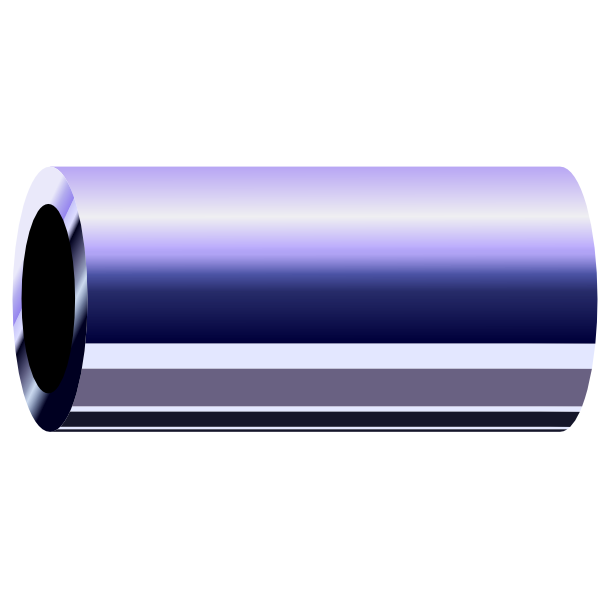
\includegraphics[width=3cm, bb=0 0 1701 1701]{graphics/misc/pipe_600x600}
\end{figure*}

The first thing one must do when relax is launched is to create a data pipe.  When using the GUI, a base data pipe will be created when opening one of the automatic analyses via the analysis selection window (see figure~\ref{fig: screenshot: analysis wizard} on page~\pageref{fig: screenshot: analysis wizard}).  This will also create a data pipe bundle for the analysis (\textit{vide infra}).  Alternatively the data pipe editor window can be used to create data pipes (see figure~\ref{fig: screenshot: pipe editor} on page~\pageref{fig: screenshot: pipe editor}).  For the prompt/scripting modes, or the \guimenuitemthree{User functions}{pipe}{create} menu entry, a data pipe can be initialised by specifying the unique name of the data pipe and the data pipe type:

\example{pipe.create(pipe\_name=`NOE 1200 MHz', pipe\_type=`noe')}

A number of relax operations will also create data pipes by merging a group of pipes or branching pre-existing pipes.  See section~\ref{sect: the data pipe} on page~\pageref{sect: the data pipe} for additional details.

All data not associated with spin systems will be stored in the base data pipe.  This includes information such as global optimisation statistics, diffusion tensors, alignment tensors, 3D structural data, the molecule, residue and spin container data structure and the interatomic data containers.  One data pipe from the set will be defined as being the current data pipe, and all operations in relax will effect data from this pipe.  The \uf{pipe.switch} user function in all UI modes can be used to change which pipe is the current data pipe.  In the GUI, switching between analysis tabs will automatically switch the current data pipe to match the analysis being displayed.


% Data pipe bundles.
\subsubsection{Data pipe bundles} \label{sect: data pipe bundles}

\begin{figure*}[h]
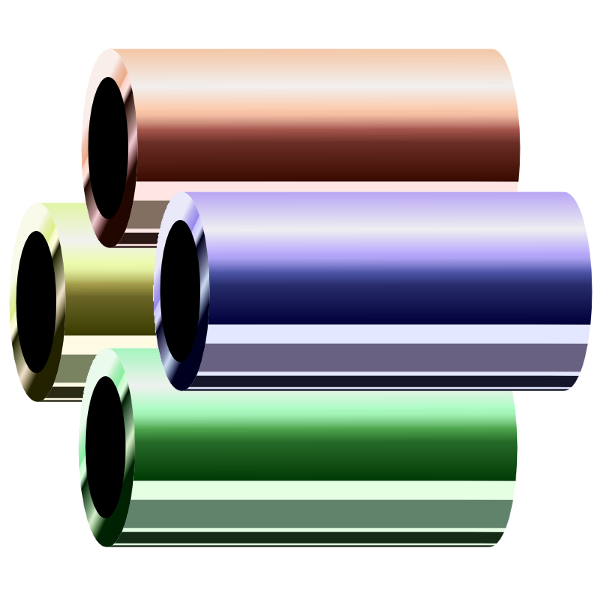
\includegraphics[width=3cm, bb=0 0 1701 1701]{graphics/misc/pipe_bundle_600x600}
\end{figure*}

Related data pipes can be grouped into a `bundle'.  For example if the data pipes ``sphere'', ``oblate spheroid'', ``prolate spheroid'', and ``ellipsoid'' preexist, these can be grouped into a bundle called ``diffusion tensors'' with the following series of user function calls:

\begin{exampleenv}
pipe.bundle(bundle=`diffusion tensors', pipe=`sphere') \\
pipe.bundle(bundle=`diffusion tensors', pipe=`oblate spheroid') \\
pipe.bundle(bundle=`diffusion tensors', pipe=`prolate spheroid') \\
pipe.bundle(bundle=`diffusion tensors', pipe=`ellipsoid')
\end{exampleenv}

The data pipe editor window of the GUI can also be used to bundle pipes together (see figure~\ref{fig: screenshot: pipe editor} on page~\pageref{fig: screenshot: pipe editor}).



% Molecule, residue, and spin containers.
%~~~~~~~~~~~~~~~~~~~~~~~~~~~~~~~~~~~~~~~~

\subsection{Molecule, residue, and spin containers}

Within a data pipe is the molecule, residue, and spin container data structure.  Data which is specific to a given nucleus is stored in a special spin container structure.  This includes relaxation data, model-free parameters, reduced spectral density mapping values, spin specific optimisation parameters, chemical shift tensor information, pseudo-contact shift values, etc.  The spin containers can be created from 3D structural data or a sequence file, as described in the next two sections, or manually built.



% Molecule containers.
\subsubsection{Molecule containers}

\begin{figure*}[h]
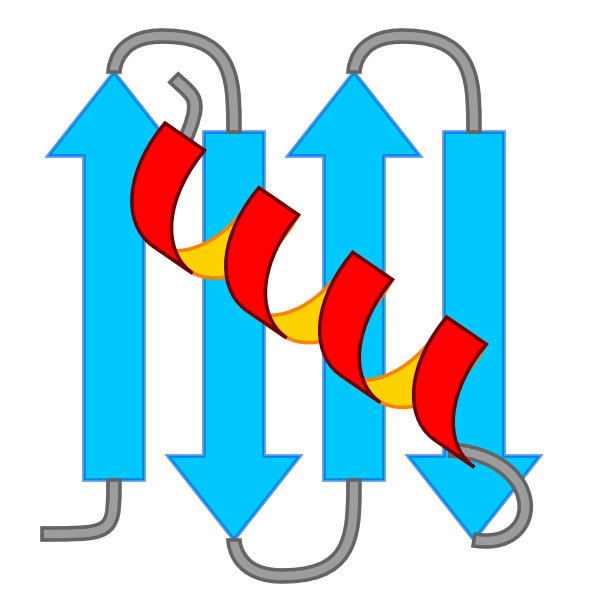
\includegraphics[width=3cm, bb=0 0 1701 1701]{graphics/misc/molecule_600x600}
\end{figure*}

The spin containers are part of a nested set of containers, and are graphically depicted in the spin viewer window of the GUI in figure~\ref{fig: screenshot: spin viewer} on page~\pageref{fig: screenshot: spin viewer}.  As can be seen from the figure, the top level holds a single molecular container.  Multiple molecular containers can be present if the study is of a molecular complex.  Using the GUI menus or the prompt/scripting mode, molecule containers can be manually created with the user function:

\example{molecule.create(mol\_name=`glycerol', mol\_type=`organic molecule')}

In the spin viewer window of the GUI, right clicking on the \gui{Spin system information} element will pop up a menu with an entry for adding molecule containers.  Right clicking on molecule containers will show a pop up menu with an entry for permanently deleting the container.



% Residue containers.
\subsubsection{Residue containers}

\begin{figure*}[h]
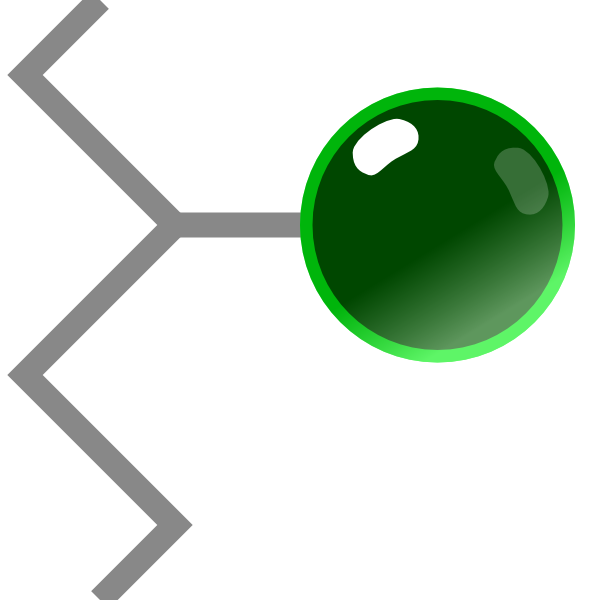
\includegraphics[width=3cm, bb=0 0 1701 1701]{graphics/misc/residue_600x600}
\end{figure*}

Nested within the molecule containers are residue containers.  These are graphically depicted in the spin viewer window (see figure~\ref{fig: screenshot: spin viewer} on page~\pageref{fig: screenshot: spin viewer}).  Each molecule container can possess multiple residues.  These require either a unique residue number or unique residue name.  For organic molecules where the residue concept is meaningless, all spin containers can be held within a single unnamed and unnumbered residue container.  Using the GUI menus or the prompt/scripting mode, residue containers can be manually created with the user function:

\example{residue.create(res\_num=`-5', res\_name=`ASP')}

Alternatively residues can be added in the spin viewer window from the pop up menu when right clicking on molecule containers, and can be deleted via the pop up menu when right clicking on the residue to delete.



% Spin containers.
\newpage
\subsubsection{Spin containers}

\begin{figure*}[h]
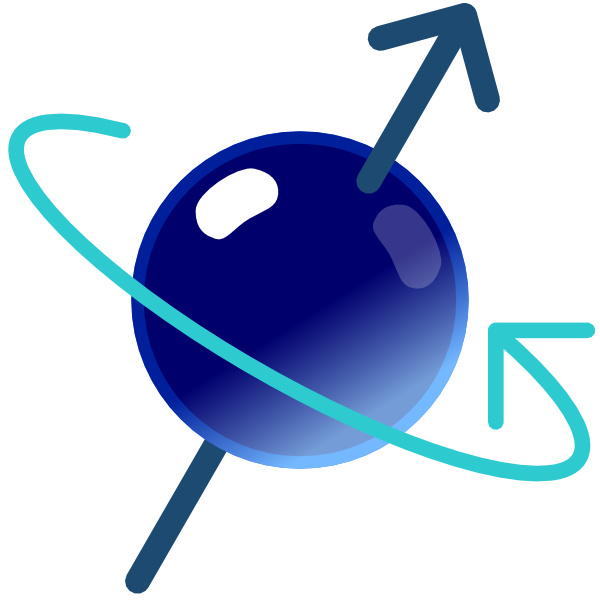
\includegraphics[width=3cm, bb=0 0 1701 1701]{graphics/misc/spin_600x600}
\end{figure*}

Spin containers are nested within a residue container (again graphically depicted in the spin viewer window in figure~\ref{fig: screenshot: spin viewer} on page~\pageref{fig: screenshot: spin viewer}).  Multiple spin containers can exist per residue.  This allows, for example, a single model-free analysis simultaneously on the backbone nitrogen spins, side-chain tryptophan indole nitrogen spins and alpha carbon spins.  Or, for example, studying the pseudocontact shifts for all nitrogen, carbon and proton spins in the molecule simultaneously.

Spin containers can be manually added via the \uf{spin.create} user function in the GUI or prompt/scripting mode:

\example{spin.create(spin\_num=`200', spin\_name=`NE1')}

The spin viewer window can also be used by right clicking on residue containers.



% Spin ID strings.
\subsubsection{Spin ID strings} \label{sect: spin ID}

Spins are often identified in relax using their ID strings.  The spin ID strings follow the basic construct found in a number of other NMR softwares such as MOLMOL.  The identification string is composed of three components:

\begin{itemize}
\item The molecule ID token beginning with the \promptstring{\#} character,
\item The residue ID token beginning with the \promptstring{:} character,
\item The atom or spin system ID token beginning with the \promptstring{@} character.
\end{itemize}

Each token can be composed of multiple elements -- one per spin -- separated by the \promptstring{,} character and each individual element can either be a number (which must be an integer, in string format), a name, or a range of numbers separated by the \promptstring{-} character.  Negative numbers are supported.  The full ID string specification is \promptstring{\#<mol\_name> :<res\_id>[, <res\_id>[, <res\_id>, ...]] @<atom\_id>[, <atom\_id>[, <atom\_id>, ...]]}, where the token elements are \promptstring{<mol\_name>}, the name of the molecule, \promptstring{<res\_id>}, the residue identifier which can be a number, name, or range of numbers, \promptstring{<atom\_id>}, the atom or spin system identifier which can be a number, name, or range of numbers.

If one of the tokens is left out then all elements will be assumed to match.  For example if the string does not contain the \promptstring{\#} character then all molecules will match the string.  If only the molecule ID component is specified, then all spins of the molecule will match.

Regular expression can, in some instances, be used to select spins.  For example the string \promptstring{@H*} will select the protons `H', `H2' and `H98'.



% Interatomic data containers.
%%%%%%%%%%%%%%%%%%%%%%%%%%%%%%

\section{Interatomic data containers} \label{sect: interatomic container}

\begin{figure*}[h]
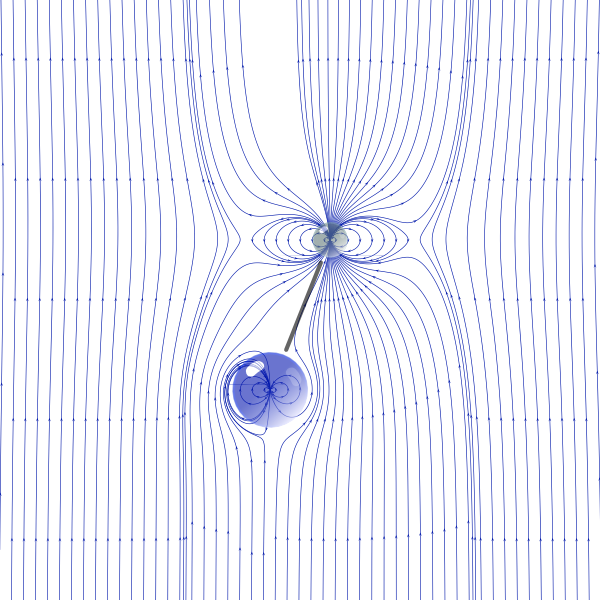
\includegraphics[width=3cm, bb=0 0 1701 1701]{graphics/wizards/dipole_pair/NH_dipole_pair_600x600}
\end{figure*}

Separate from the spin containers, yet strongly linked to them, are the interatomic data containers.  These containers are grouped together within the same data pipe as the spins they point to.  These define interactions between two spins located anywhere within the molecule, residue and spin nested data structure.  These are automatically created when reading in data defined between two spins such as RDCs and NOE distance constraints.  They can also be created using the \uf{interatom.define} user function:

\example{interatom.define(spin\_id1=`:2@N', spin\_id2=`:2@H')}

As the interatomic data container concept is relatively new, how they are created and handled is likely to evolve and change in the future.



% Setup in the prompt/script UI.
%%%%%%%%%%%%%%%%%%%%%%%%%%%%%%%%

\section{Setup in the prompt/script UI}

Below are three different examples showing how to set up the relax data model for any analysis type requiring spin specific data.


% Spins from structural data.
%~~~~~~~~~~~~~~~~~~~~~~~~~~~~

\subsection{Script mode -- spins from structural data} \label{sect: script - structural data}

\begin{figure*}[h]
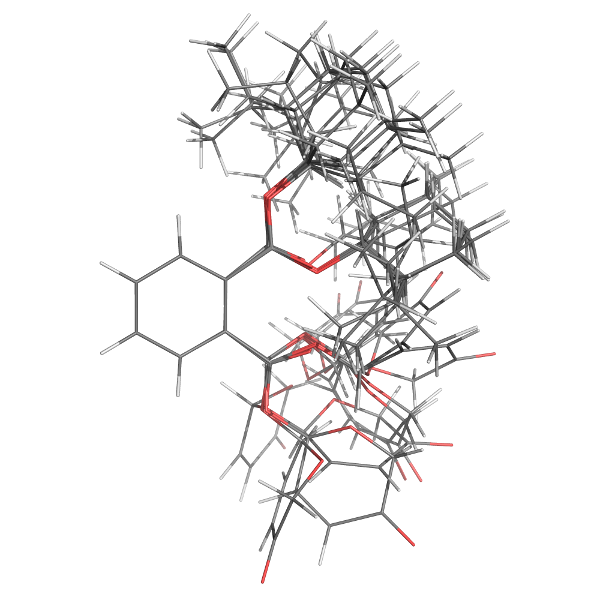
\includegraphics[width=3cm, bb=0 0 1701 1701]{graphics/misc/n_state_model/phthalic_acid_ens_600x600}
\end{figure*}

3D structural data is stored at the level of the current data pipe.  This data is completely separate from the molecule, residue and spin data structure.  However the structural data can be used to generate the spin containers.  For example for the nitrogen relaxation in a model-free analysis where both the nitrogen and proton are needed to define the magnetic dipole-dipole relaxation:

\begin{exampleenv}
\# Create a data pipe. \\
pipe.create(pipe\_name=`ellipsoid', pipe\_type=`mf') \\
 \\
\# Load the PDB file. \\
structure.read\_pdb(`1f3y.pdb') \\
 \\
\# Set up the 15N and 1H backbone spins. \\
structure.load\_spins(`@N', ave\_pos=True) \\
structure.load\_spins(`@H', ave\_pos=True) \\
 \\
\# Set up the 15N and 1H for the tryptophan indole ring. \\
structure.load\_spins(`@NE1', ave\_pos=True) \\
structure.load\_spins(`@HE1', ave\_pos=True) \\
 \\
\# Define the spin isotopes. \\
spin.isotope(`15N', spin\_id=`@N*') \\
spin.isotope(`1H', spin\_id=`@H*')
\end{exampleenv}

The \uf{structure.read\_pdb} user function will load the structural data into the current data pipe, and the \uf{structure.load\_spins} user function will create the molecule, residue, and spin containers as needed.  This will also load atomic position information into the matching spin containers.  The \uf{spin.isotope} user function is required to define the magnetic dipole-dipole interaction and is information not present in the PDB file.

Note that if structural data from the PDB is used to generate the spin containers, then all subsequent data loaded into relax must follow the exact naming convention from the PDB file.  Automatic residue name matching (i.e. `GLY' = `Gly' = `gly' = `G') is currently not supported.



% Spins from a sequence file.
%~~~~~~~~~~~~~~~~~~~~~~~~~~~~

\subsection{Script mode -- spins from a sequence file} \label{sect: script - sequence file}

\begin{figure*}[h]
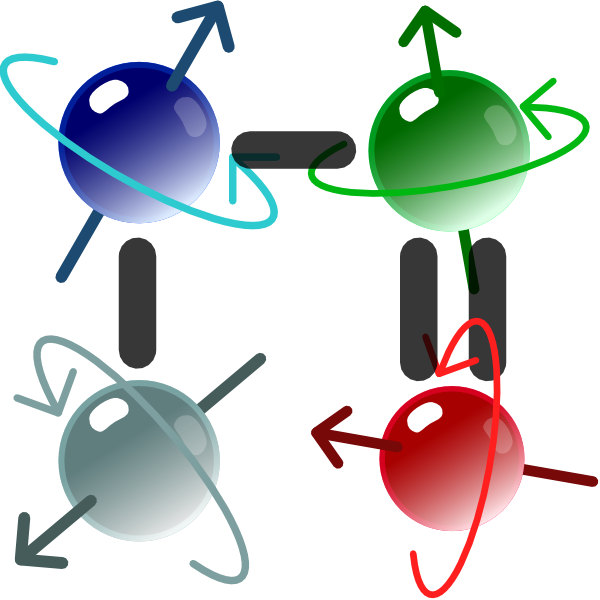
\includegraphics[width=3cm, bb=0 0 1701 1701]{graphics/misc/sequence_600x600}
\end{figure*}

Alternatively to setting up the molecule, residue, and spin containers via 3D structural data, a plain text columnar formatted file can be used.  This is useful for when no 3D structure exists for the molecule.  It also has the advantage that the residue and atom names need not conform to the PDB standard.  An example for reading sequence data is:

\begin{exampleenv}
\# Create a data pipe. \\
pipe.create(pipe\_name=`R1 1200', pipe\_type=`relax\_fit') \\
 \\
\# Set up the 15N spins. \\
sequence.read(file=`noe.500.out', mol\_name\_col=1, res\_num\_col=2, res\_name\_col=3, spin\_num\_col=4, spin\_name\_col=5) \\
spin.element(element=`N', spin\_id=`@N*') \\
spin.isotope(`15N', spin\_id=`@N')
\end{exampleenv}

Here the molecule, residue, and spin information is extracted from the \promptstring{noe.500.out} file which could look like:

{\scriptsize \begin{verbatim}
# mol_name          res_num  res_name  spin_num  spin_name  value             error               
Ap4Aase_new_3_mol1  1        GLY       1         N          None              None                
Ap4Aase_new_3_mol1  2        PRO       11        N          None              None                
Ap4Aase_new_3_mol1  3        LEU       28        N          None              None                
Ap4Aase_new_3_mol1  4        GLY       51        N          0.03892194698453  0.01903177024613    
Ap4Aase_new_3_mol1  5        SER       59        N          0.31240422567912  0.01859693729836    
Ap4Aase_new_3_mol1  6        MET       71        N          0.42850831873249  0.0252585632304     
Ap4Aase_new_3_mol1  7        ASP       91        N          0.53054928103134  0.02799062314416    
Ap4Aase_new_3_mol1  8        SER       104       N          0.56528429775819  0.02170612146773    
Ap4Aase_new_3_mol1  9        PRO       116       N          None              None                
Ap4Aase_new_3_mol1  40       TRP       685       N          0.65394813490548  0.03830061886537    
Ap4Aase_new_3_mol1  40       TRP       698       NE1        0.67073879732046  0.01426066343831    
\end{verbatim}} \label{verb: noe.500.out}

The file can contain columns for the molecule name, the residue name and number, and the spin name and number in any order though not all are needed.  For example for a single protein system, the molecule name, residue name and spin number are nonessential.  Or for an organic molecule, the molecule name, residue name and number and spin number could be nonessential.  The subsequent user functions in the above example are used to set up the spin containers appropriately for a model-free analysis.  These are not required in the automatic analysis of GUI as these user functions will be presented to you when adding relaxation data, or when clicking on the heteronucleus and proton buttons (\guibutton{X isotope} and \guibutton{H isotope}).

In the GUI, the creation of molecule, residue, and spin containers from a sequence file is also available via the \gui{Load spins} wizard within the spin viewer window (\textit{vide supra}).


% Manual construction.
%~~~~~~~~~~~~~~~~~~~~~

\subsection{Script mode -- manual construction} \label{sect: script - manual construction}

For the masochists out there, the full molecule, residue and spin data structure can be manually constructed.  For example:

\begin{exampleenv}
\# Manually create the molecule, residue, and spin containers. \\
molecule.create(mol\_name=`Ap4Aase', mol\_type=`protein') \\
residue.create(res\_num=1,  res\_name=`GLY') \\
residue.create(res\_num=3,  res\_name=`LEU') \\
residue.create(res\_num=96, res\_name=`TRP') \\
spin.create(res\_num=1,  spin\_name=`N') \\
spin.create(res\_num=3,  spin\_name=`N') \\
spin.create(res\_num=96, spin\_name=`N') \\
spin.create(res\_num=96, spin\_name=`NE1')
\end{exampleenv}

These user functions can be repeated until the full sequence has been constructed.



% Setup in the GUI.
%%%%%%%%%%%%%%%%%%%

\section{Setup in the GUI}


% The data pipe.
%~~~~~~~~~~~~~~~

\subsection{GUI mode -- setting up the data pipe} \label{sect: GUI - data pipe}

In the GUI, the most common way to create the data pipe is to initialise one of the auto-analyses via the analysis selection wizard (see Figure~\ref{fig: screenshot: analysis wizard} on page~\pageref{fig: screenshot: analysis wizard}).  The initialisation will create the appropriate starting data pipe.  Alternatively the data pipe editor can be used (see Figure~\ref{fig: screenshot: pipe editor} on page~\pageref{fig: screenshot: pipe editor}).  Or the \guimenuitemthree{User functions}{pipe}{create} menu item can be selected for graphical access to the \uf{pipe.create} user function.



% Spins from structural data.
%~~~~~~~~~~~~~~~~~~~~~~~~~~~~

\subsection{GUI mode -- spins from structural data} \label{sect: GUI - structural data}

For this section, the example of protein $^{15}$N relaxation data will be used to illustrate how to set up the data structures.  To manipulate the molecule, residue and spin data structures in the GUI, the most convenient option is to use the spin viewer window (see Figure~\ref{fig: screenshot: spin viewer} on page~\pageref{fig: screenshot: spin viewer}).  This window can be opened in four ways:

\begin{itemize}
\item The \guimenuitemtwo{View}{Spin viewer} menu item,
\item The \shortcutkey{Ctrl+T} key combination,
\item The spin viewer icon in the toolbar (represented by the blue spin icon),
\item The \guibutton{Spin editor} button part of the \gui{Spin systems} GUI element in the specific analysis tabs.
\end{itemize}

You will then see:

\begin{minipage}[h]{\linewidth}
\centerline{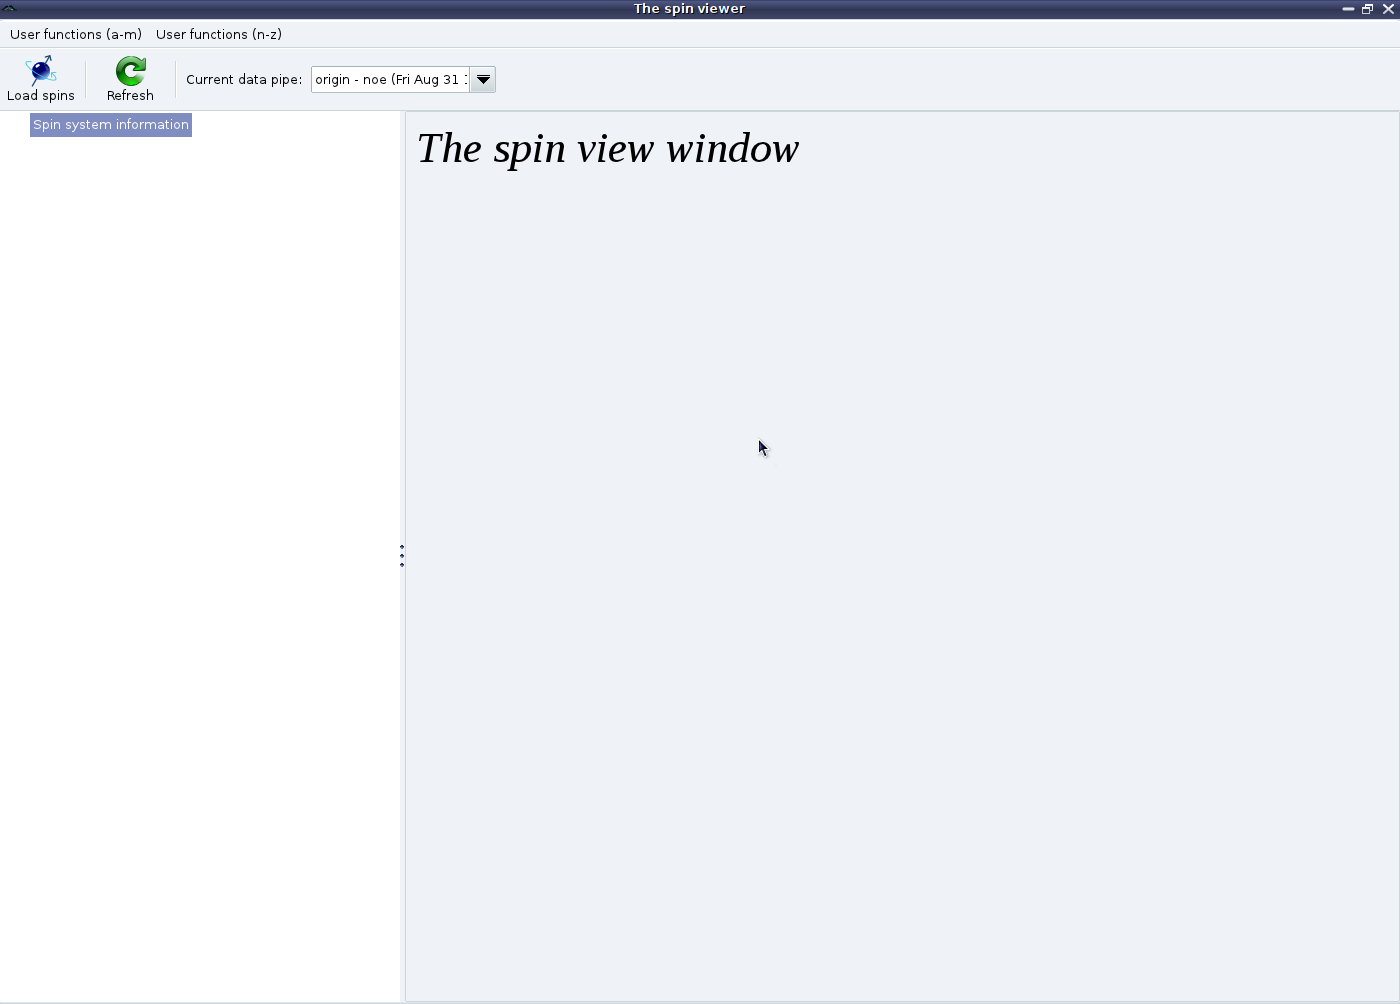
\includegraphics[width=0.8\textwidth, bb=14 14 1415 1019]{graphics/screenshots/spin_viewer/blank}}
\label{figure: spin viewer blank}
\end{minipage}

At this point, click on the \guibutton{Load spins} button (or the \guimenuitemone{Load spins} menu entry from the right click pop up menu) to launch the spin loading wizard.  A number of options will be presented to you: 

\begin{minipage}[h]{\linewidth}
\centerline{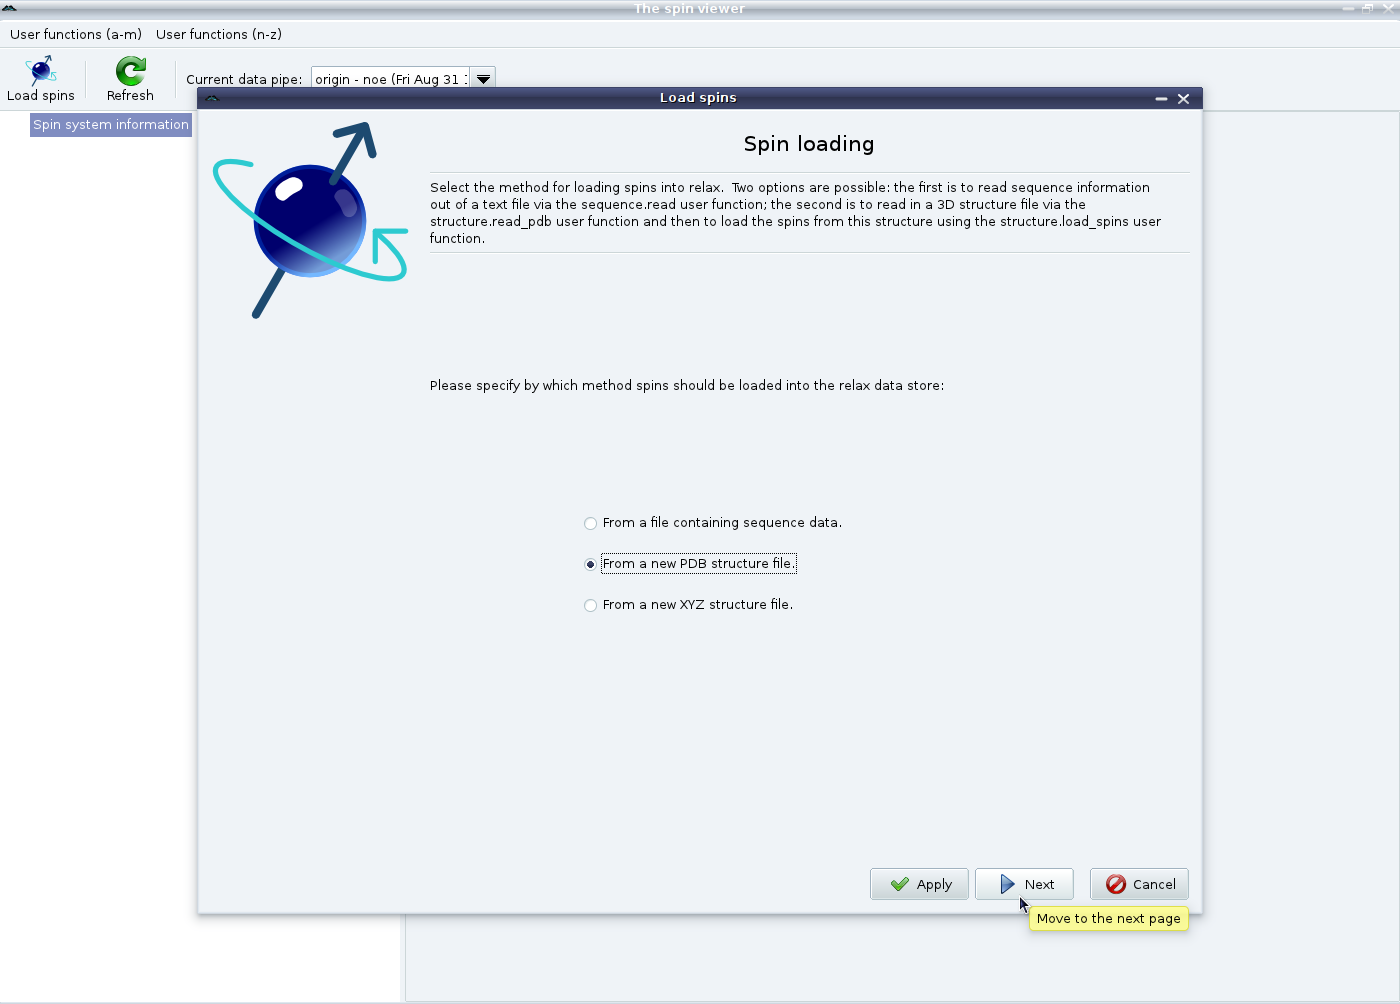
\includegraphics[width=0.8\textwidth, bb=14 14 1415 1019]{graphics/screenshots/spin_viewer/wizard_start}}
\label{figure: spin viewer wizard start}
\end{minipage}

Here the spins will be loaded from a PDB file.  If you do not have a 3D structure file, please see the next section.  After selecting \gui{From a new PDB structure file} and clicking on \guibutton{Next}, you will see:

\begin{minipage}[h]{\linewidth}
\centerline{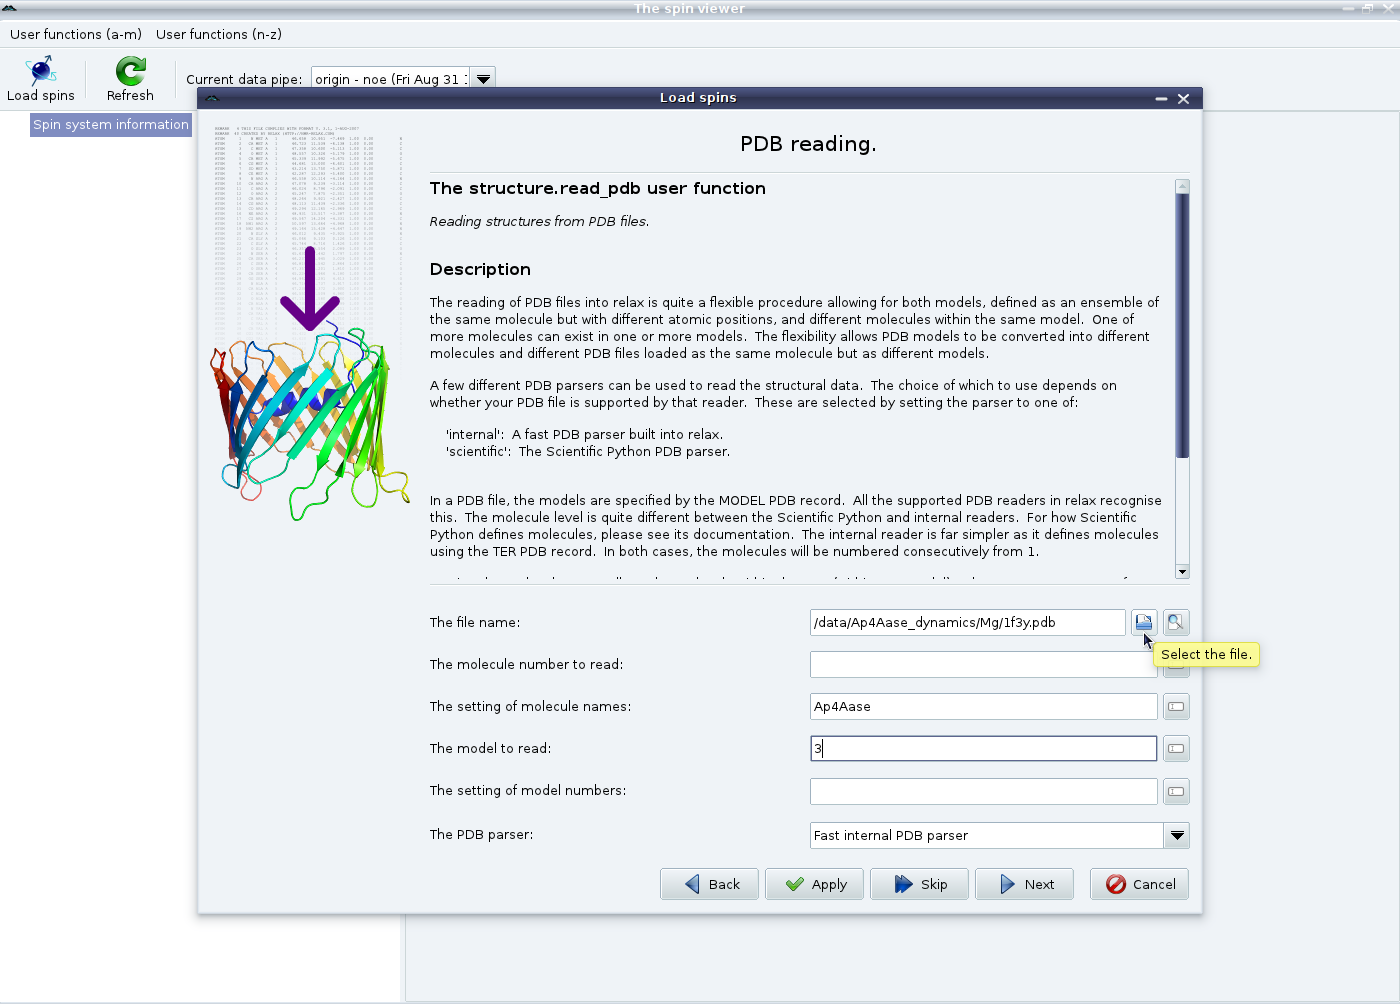
\includegraphics[width=0.8\textwidth, bb=14 14 1415 1019]{graphics/screenshots/spin_viewer/wizard_read_pdb}}
\end{minipage}

Now select the PDB file you wish to use.  The other options in this screen allow you to handle NMR models and multiple molecules within a single PDB file.  These options are explained in the window.  Hovering the mouse over the options will give additional hints.  In this example, the \nth{3} model from the 1F3Y PDB file will be read and the single molecule will be named \guistring{Ap4Aase} to override the default naming of \guistring{1f3y\_mol1}.  Now click on \guibutton{Next} to bring up the spin loading page:

\begin{minipage}[h]{\linewidth}
\centerline{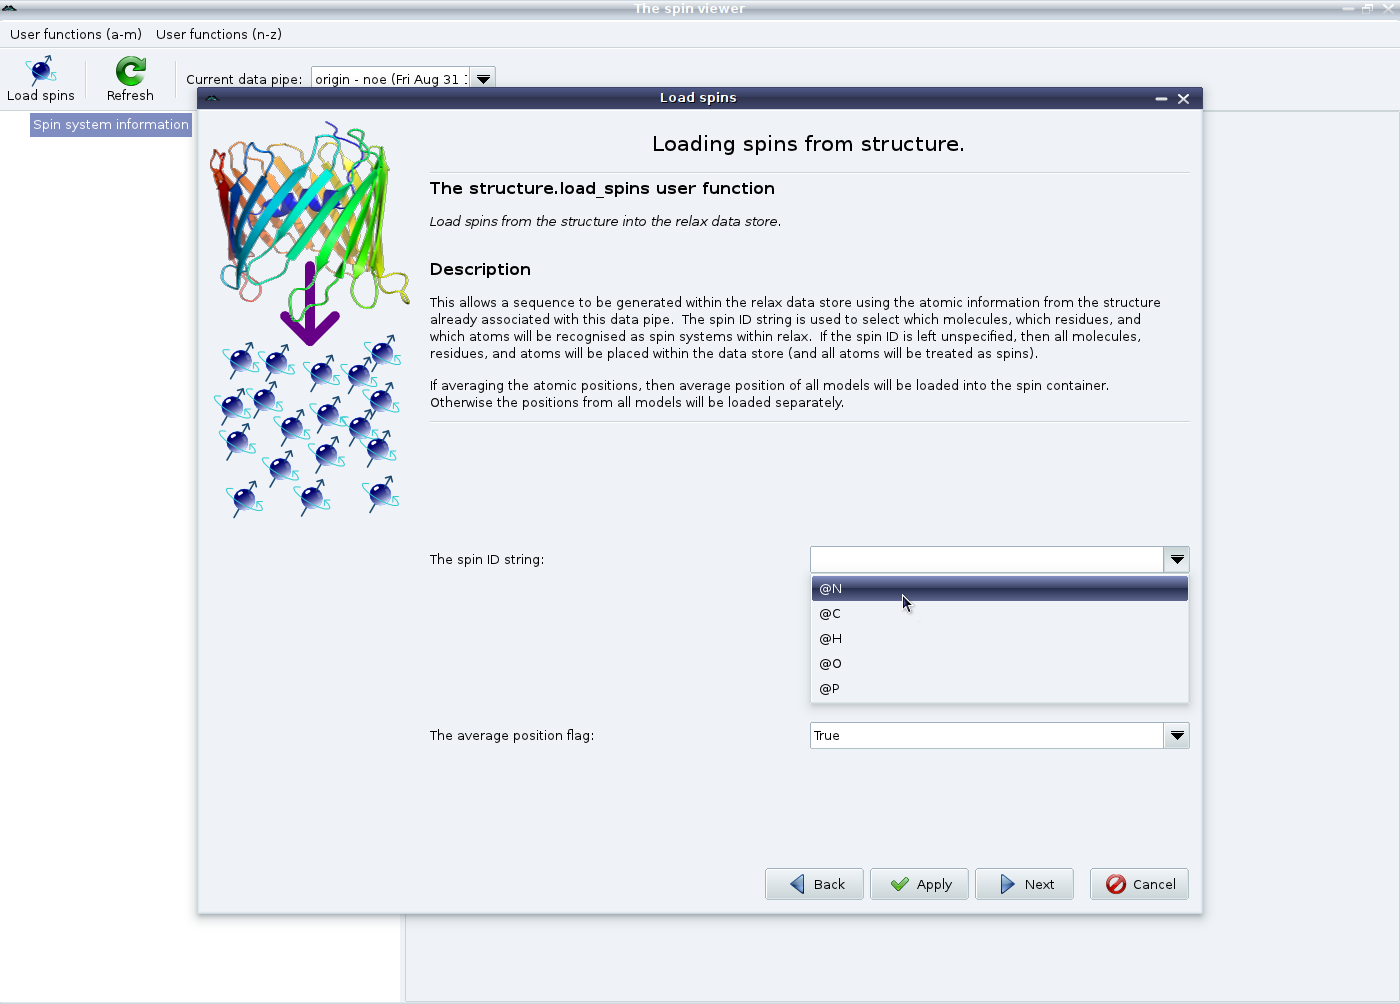
\includegraphics[width=0.8\textwidth, bb=14 14 1415 1019]{graphics/screenshots/spin_viewer/wizard_load_spins_n}}
\end{minipage}

This is a bit more complicated.  In this example we are studying the backbone dynamics of $^{15}$N spins of a protein.  Therefore first set the spin ID string to \guistring{@N} (which can be selected from the pull down) and click on \guibutton{Apply} to set up the backbone spins.  Do not click on \guibutton{Next} yet.  If the current study requires the specification of the dipole-dipole interaction (for example if it involves relaxation data -- model-free analyses, consistency testing, reduced spectral density mapping; or the dipolar coupling -- the N-state model or ensemble analyses, the Frame Order theory) you will also need to load the $^1$H spins as well.  Therefore set the spin ID string to \guistring{@H} and click on \guibutton{Apply} again.


\begin{minipage}[h]{\linewidth}
\centerline{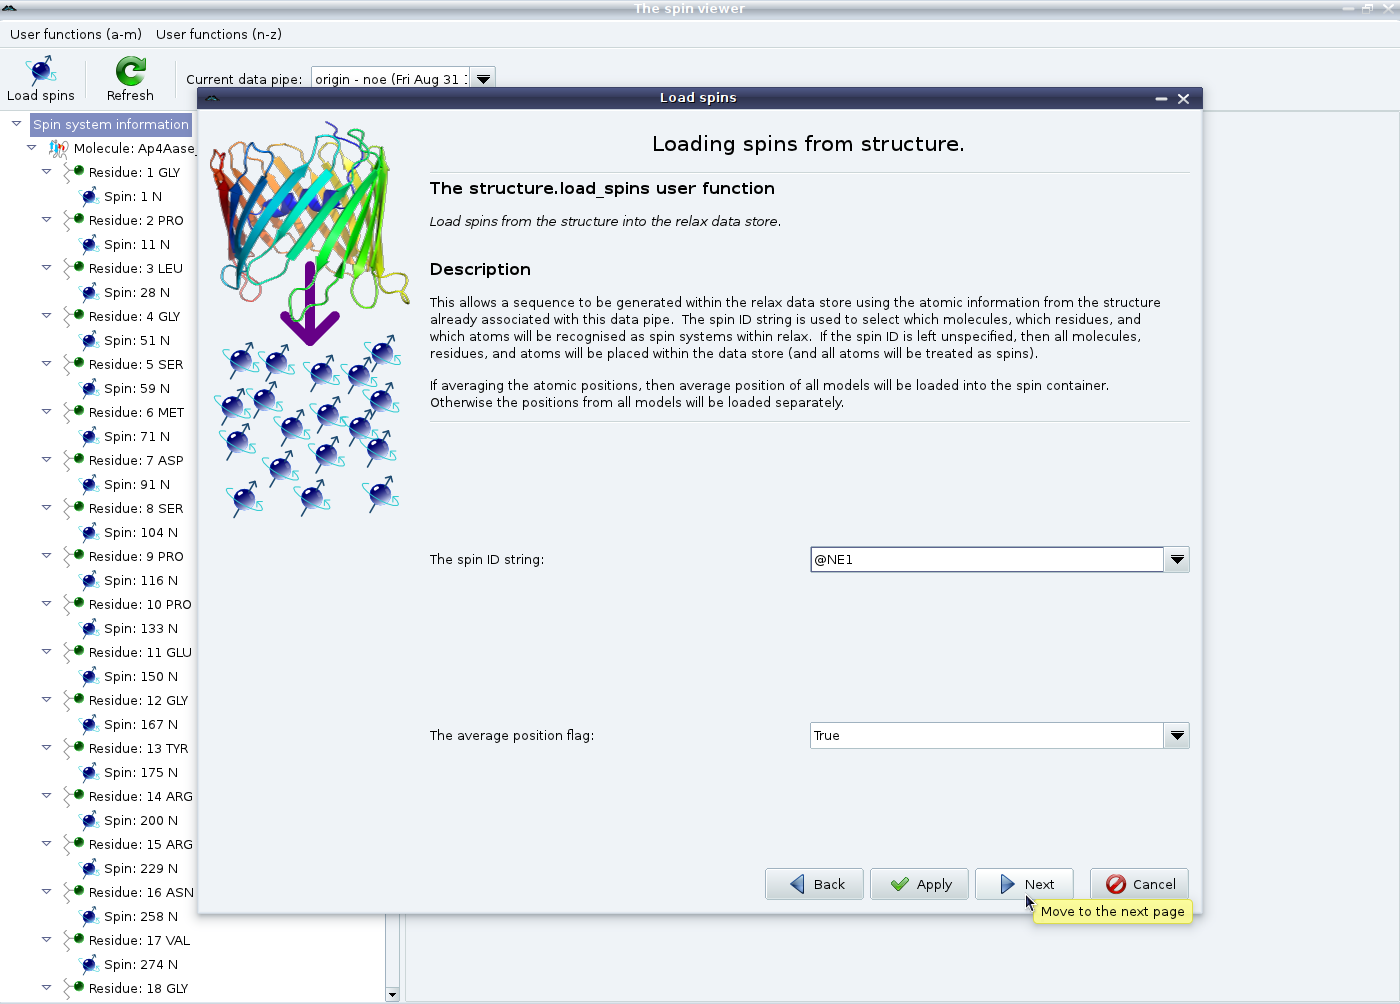
\includegraphics[width=0.8\textwidth, bb=14 14 1415 1019]{graphics/screenshots/spin_viewer/wizard_load_spins_ne1}}
\end{minipage}

Now change the spin ID string to \guistring{@NE1} and then click on \guibutton{Next} (or \guibutton{Apply} if the Trp protons \guistring{@HE1} need to be loaded as well).  This will add spin containers for the tryptophan indole $^{15}$N spins.  Finally click on \guibutton{Finish} to exit the wizard:

\begin{minipage}[h]{\linewidth}
\centerline{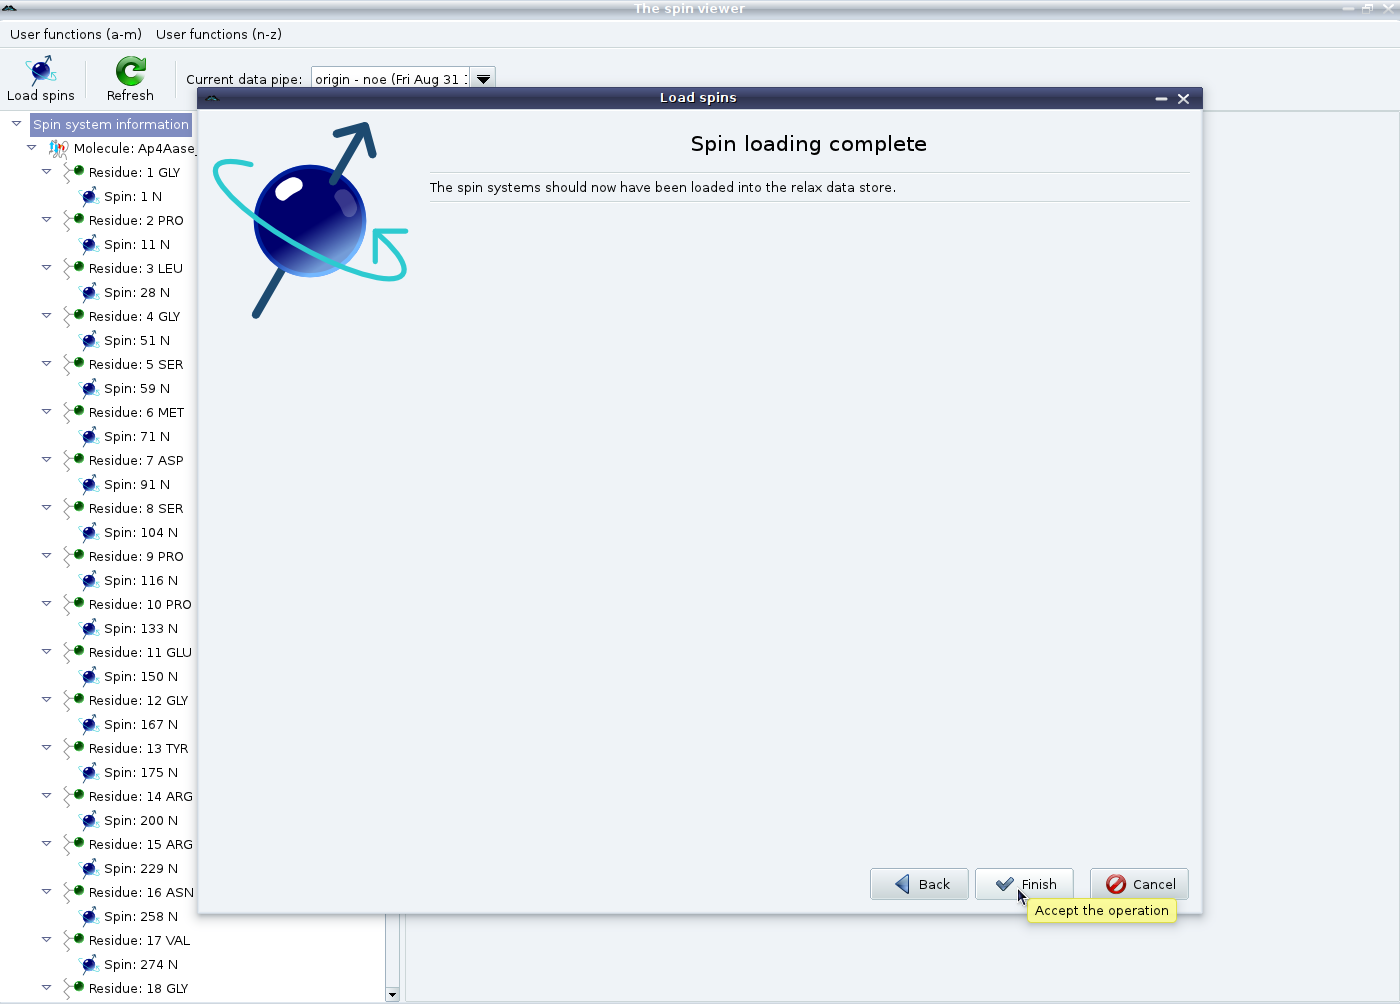
\includegraphics[width=0.8\textwidth, bb=14 14 1415 1019]{graphics/screenshots/spin_viewer/wizard_end}}
\label{figure: spin viewer end}
\end{minipage}

You should now see something such as:

\begin{minipage}[h]{\linewidth}
\centerline{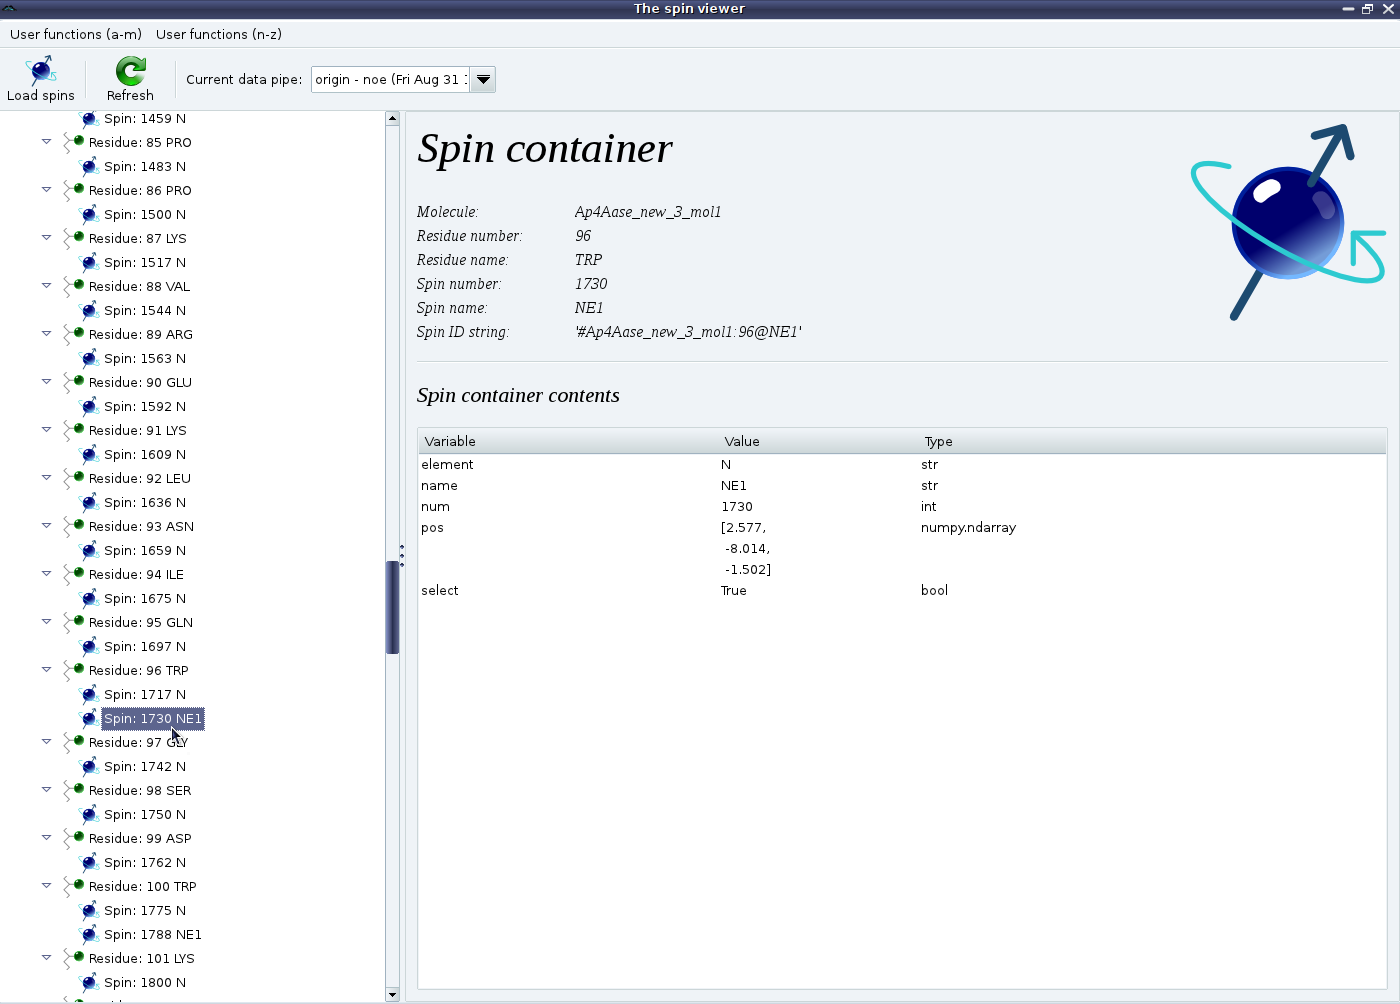
\includegraphics[width=0.8\textwidth, bb=14 14 1415 1019]{graphics/screenshots/spin_viewer/full}}
\end{minipage}

If the $^1$H spins have been loaded as well, then you should see exactly twice as many spin containers as shown above.


% Spins from a sequence file.
%~~~~~~~~~~~~~~~~~~~~~~~~~~~~

\subsection{GUI mode -- spins from a sequence file} \label{sect: GUI - sequence file}

Starting from the empty spin viewer window on page~\pageref{figure: spin viewer blank}), click on the \guibutton{Load spins} button.  You will then see the spin loading wizard (see page~\pageref{figure: spin viewer wizard start}).  Select the option for reading data from a sequence file.  You should then see:

\begin{minipage}[h]{\linewidth}
\centerline{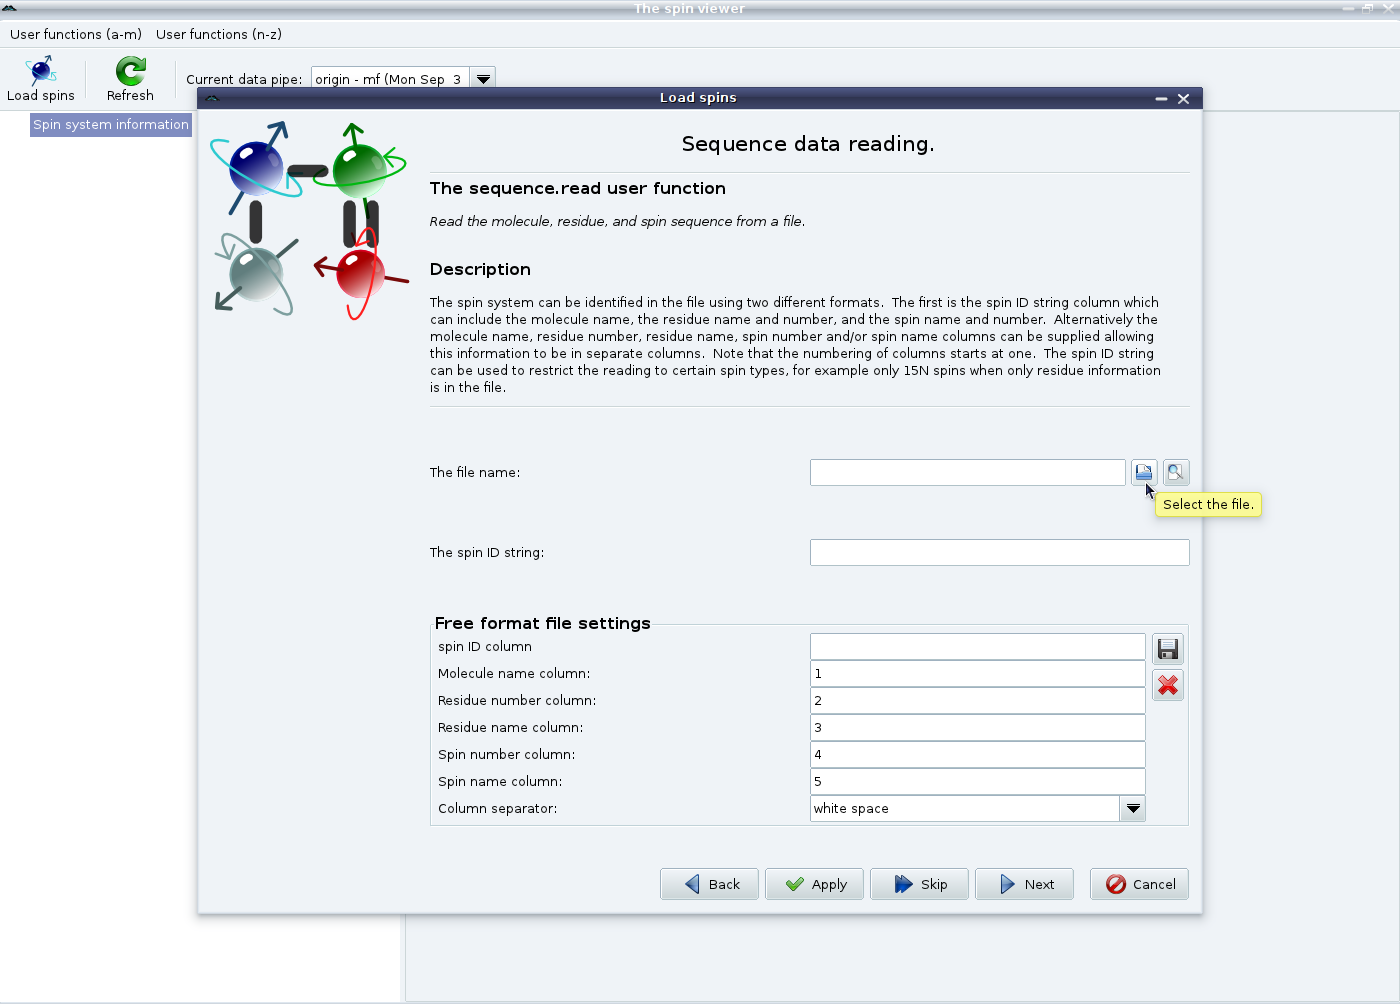
\includegraphics[width=0.8\textwidth, bb=14 14 1415 1019]{graphics/screenshots/spin_viewer/wizard_sequence}}
\end{minipage}

Select the file to load and change the \gui{Free format file settings} as needed.  An example of a suitable format is given on page~\pageref{verb: noe.500.out}.  Click on \guibutton{Next} to reach the wizard ending page (see~\pageref{figure: spin viewer end}).  Finally click on \guibutton{Finish} to exit the wizard.


% Manual construction.
%~~~~~~~~~~~~~~~~~~~~~

\subsection{GUI mode -- manual construction} \label{sect: GUI - manual construction}

Just as in the prompt/script UI mode, the molecules, residues and spins can be manually added.  First add a molecule by right clicking on the \gui{Spin system information} element and selecting the relevant entry in the popup menu.  Then right click on the newly created molecule container to add residues, and right click on residue containers to add spins.


% Deselect spins.
%~~~~~~~~~~~~~~~~

\subsection{GUI mode -- deselect spins} \label{sect: GUI - deselect spins}

To deselect spins (for example if they are unresolved, overlapping peaks), click on the \guimenuitemthree{User functions}{deselect}{read} menu item from the main relax window or the spin viewer window:

\begin{minipage}[h]{\linewidth}
\centerline{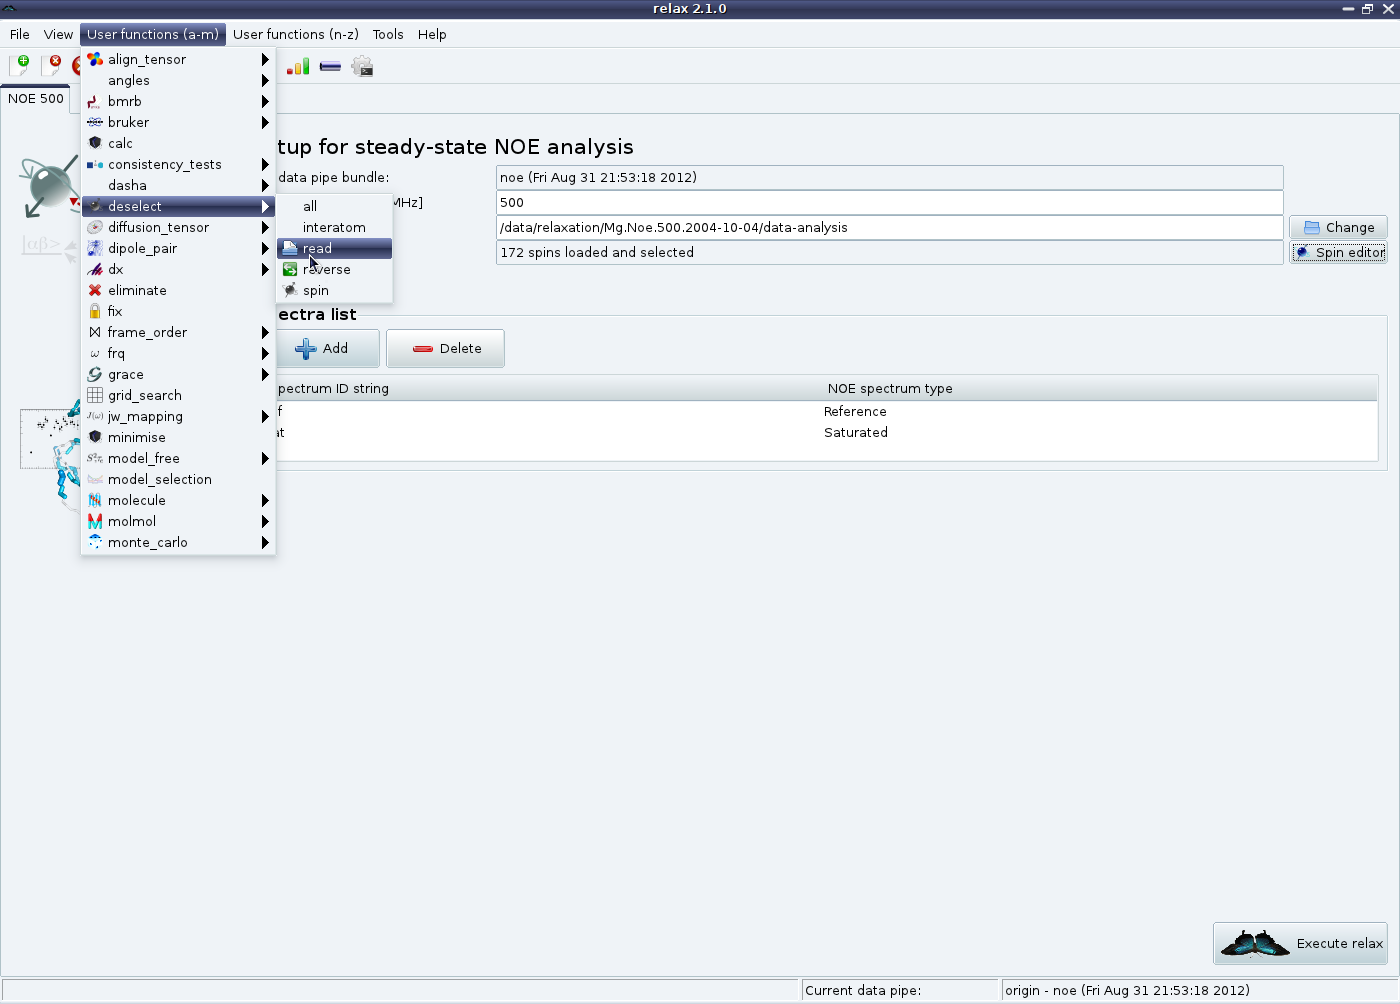
\includegraphics[width=0.8\textwidth, bb=14 14 1415 1019]{graphics/screenshots/noe_analysis/analysis_tab3}}
\end{minipage}

Select the file listing the unresolved spins and change the column numbers in the \gui{Free format file settings} GUI element as needed: 

\begin{minipage}[h]{\linewidth}
\centerline{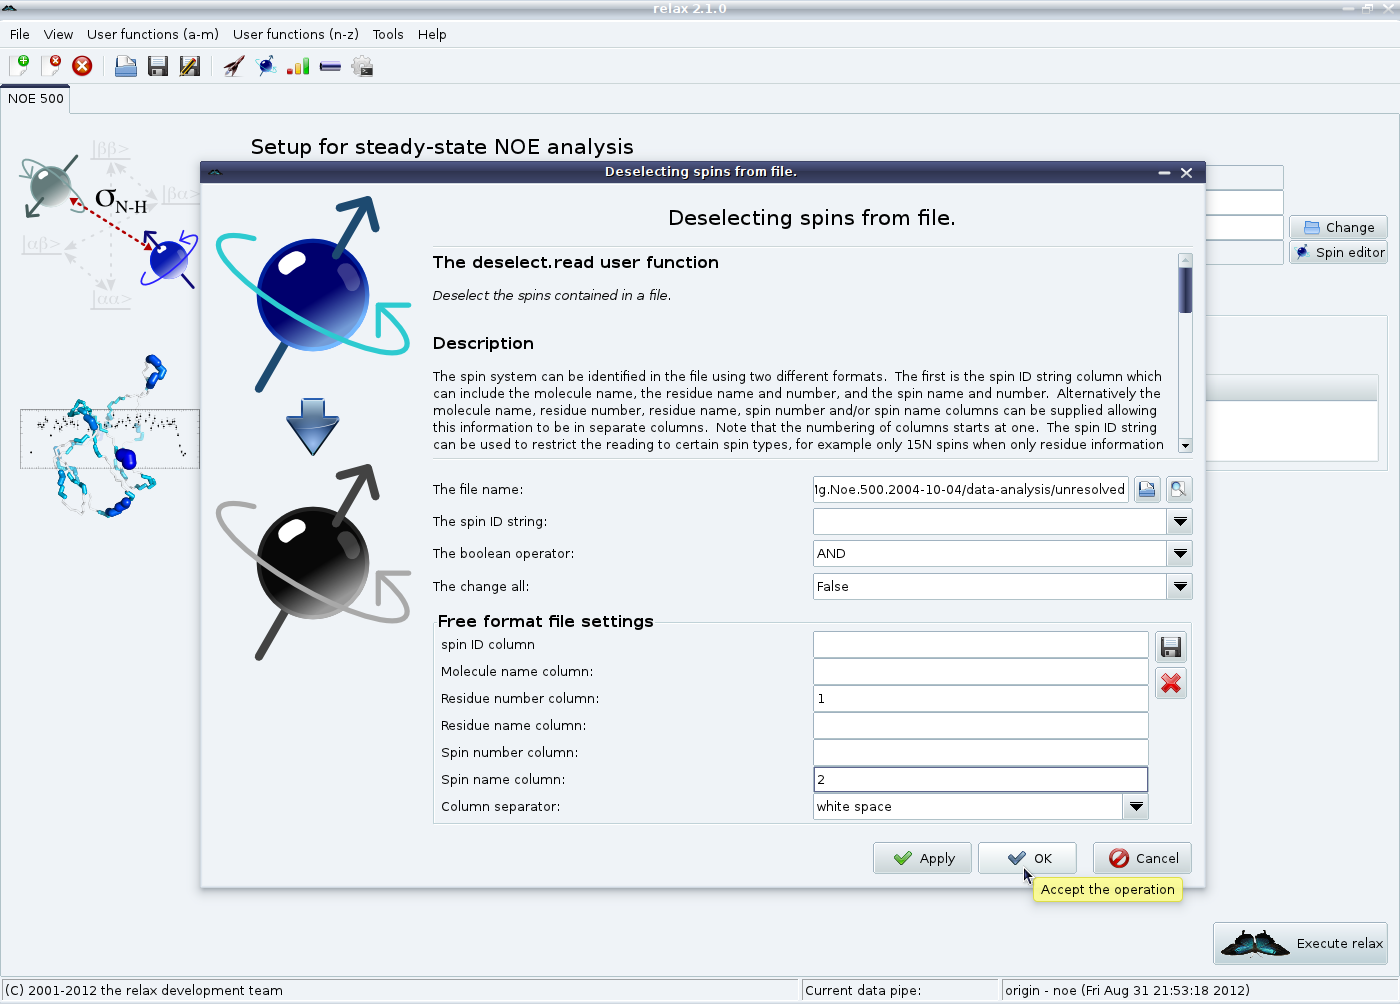
\includegraphics[width=0.8\textwidth, bb=14 14 1415 1019]{graphics/screenshots/noe_analysis/deselect}}
\end{minipage}

Alternatively the spin editor window can be reopened and the spins manually deselected by right clicking on them and selecting \gui{Deselect}.  Returning to the spin editor window, you should now see certain spins coloured grey:

\begin{minipage}[h]{\linewidth}
\centerline{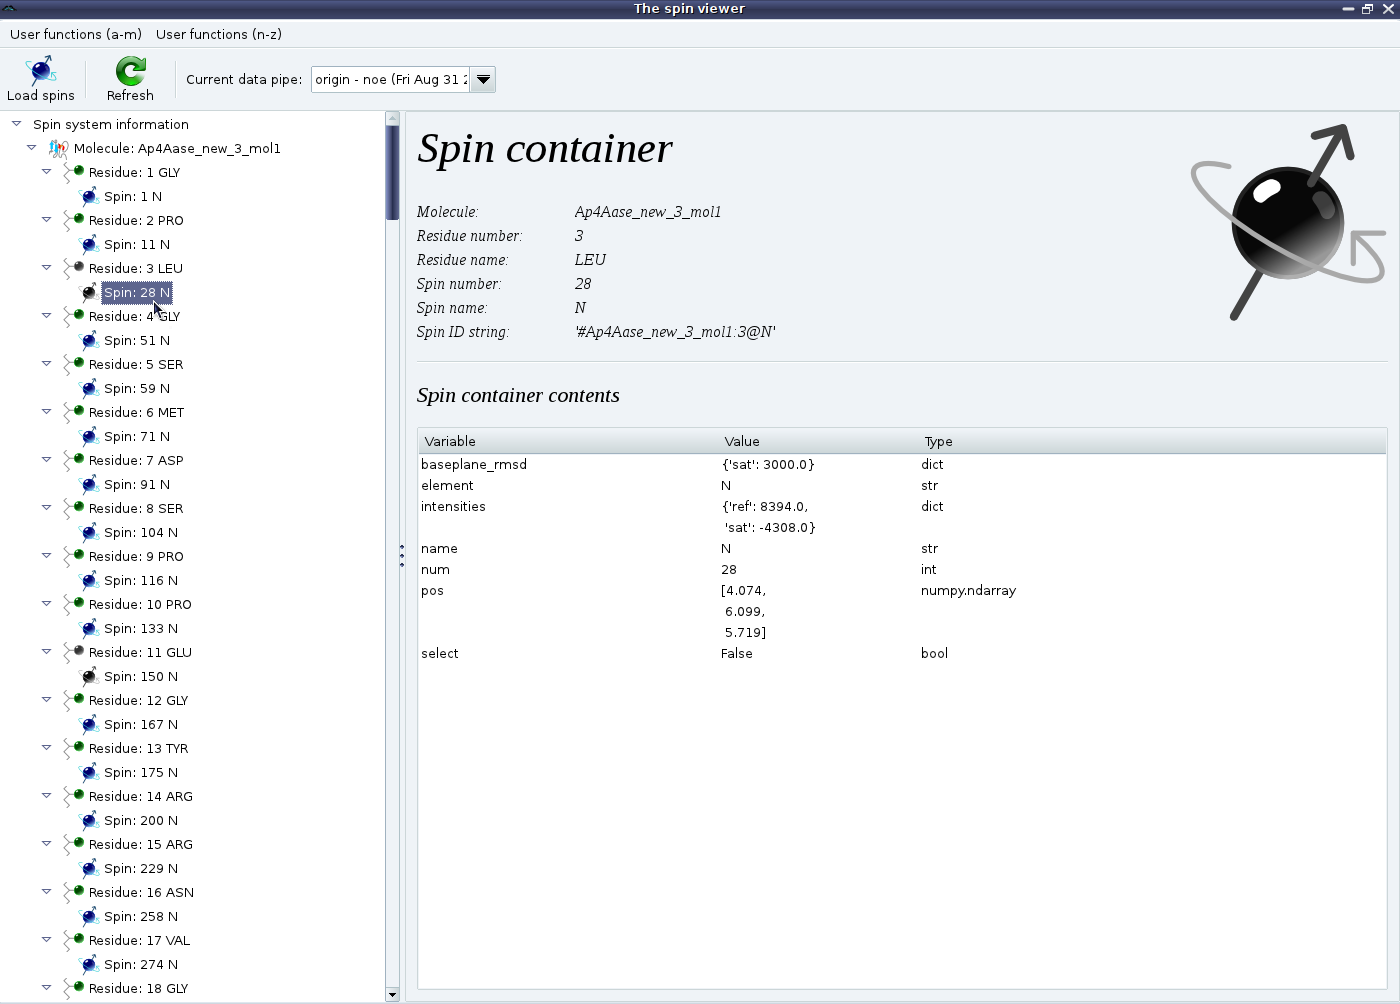
\includegraphics[width=0.8\textwidth, bb=14 14 1415 1019]{graphics/screenshots/spin_viewer/deselect}}
\end{minipage}



% The next steps.
%%%%%%%%%%%%%%%%%

\section{The next steps}

This chapter presented the basics of setting up the relax data store, concepts which are needed for all analysis types built into relax.  The next chapters will introduce specific analyses types -- the steady-state NOE, $\Rone$ and $\Rtwo$ relaxation curve-fitting, and the automated full model-free analysis protocol of \citet{dAuvergneGooley07,dAuvergneGooley08b} -- which build on the ideas introduced here.


\part{The specific analyses}
% Relaxation curve-fitting.
%%%%%%%%%%%%%%%%%%%%%%%%%%%

\chapter[Relaxation curve-fitting]{The $\Rone$ and $\Rtwo$ relaxation rates -- relaxation curve-fitting}
\index{relaxation curve-fitting|textbf}



% Introduction.
%%%%%%%%%%%%%%%

\section{Introduction}

Relaxation curve-fitting involves a number of steps including the loading of data, the calculation of both the average peak intensity\index{peak!intensity} across replicated spectra and the standard deviations\index{standard deviation} of those peak intensities, selection of the experiment type, optimisation of the parameters of the fit, Monte Carlo simulations\index{Monte Carlo simulation} to find the parameter errors, and saving and viewing the results.  To simplify the process a sample script will be followed step by step as was done with the NOE calculation.



% The sample script.
%%%%%%%%%%%%%%%%%%%%

\section{The sample script}

\begin{exampleenv}
\# Script for relaxation curve-fitting. \\
 \\
\# Create the `rx' data pipe. \\
pipe.create(`rx', `relax\_fit') \\
 \\
\# Load the backbone amide 15N spins from a PDB file. \\
structure.read\_pdb(`Ap4Aase\_new\_3.pdb') \\
structure.load\_spins(spin\_id=`@N') \\
 \\
\# Load the peak intensities. \\
relax\_fit.read(file=`T2\_ncyc1.list', relax\_time=0.0176) \\
relax\_fit.read(file=`T2\_ncyc1b.list', relax\_time=0.0176) \\
relax\_fit.read(file=`T2\_ncyc2.list', relax\_time=0.0352) \\
relax\_fit.read(file=`T2\_ncyc4.list', relax\_time=0.0704) \\
relax\_fit.read(file=`T2\_ncyc4b.list', relax\_time=0.0704) \\
relax\_fit.read(file=`T2\_ncyc6.list', relax\_time=0.1056) \\
relax\_fit.read(file=`T2\_ncyc9.list', relax\_time=0.1584) \\
relax\_fit.read(file=`T2\_ncyc9b.list', relax\_time=0.1584) \\
relax\_fit.read(file=`T2\_ncyc11.list', relax\_time=0.1936) \\
relax\_fit.read(file=`T2\_ncyc11b.list', relax\_time=0.1936) \\
 \\
\# Calculate the peak intensity averages and the standard deviation of all spectra. \\
relax\_fit.mean\_and\_error() \\
 \\
\# Deselect unresolved residues. \\
deselect.read(file=`unresolved') \\
 \\
\# Set the relaxation curve type. \\
relax\_fit.select\_model(`exp') \\
 \\
\# Grid search. \\
grid\_search(inc=11) \\
 \\
\# Minimise. \\
minimise(`simplex', scaling=False, constraints=False) \\
 \\
\# Monte Carlo simulations. \\
monte\_carlo.setup(number=500) \\
monte\_carlo.create\_data() \\
monte\_carlo.initial\_values() \\
minimise(`simplex', scaling=False, constraints=False) \\
monte\_carlo.error\_analysis() \\
 \\
\# Save the relaxation rates. \\
value.write(param=`rx', file=`rx.out', force=True) \\
 \\
\# Grace plots of the relaxation rate. \\
grace.write(y\_data\_type=`rx', file=`rx.agr', force=True) \\
grace.view(file=`rx.agr') \\
 \\
\# Save the program state. \\
state.save(file=`rx.save', force=True)
\end{exampleenv}



% Initialisation of the data pipe and loading of the data.
%%%%%%%%%%%%%%%%%%%%%%%%%%%%%%%%%%%%%%%%%%%%%%%%%%%%%%%%%%

\section{Initialisation of the data pipe and loading of the data}

The start of this sample script is very similar to that of the NOE calculation on page~\pageref{NOE initialisation}.  The command

\begin{exampleenv}
pipe.create(`rx', `relax\_fit')
\end{exampleenv}

initialises the data pipe labelled \texttt{`rx'}.  The data pipe type is set to relaxation curve-fitting by the argument \texttt{`relax\_fit'}.  The backbone amide nitrogen sequence is extracted from a PDB\index{PDB} file using the same commands as the NOE calculation script

\example{structure.read\_pdb(name, `Ap4Aase\_new\_3.pdb')}
\index{PDB}

\example{structure.load\_spins(spin\_id=`@N')}

To load the peak intensities\index{peak!intensity} into relax the user function \texttt{relax\_fit.read} is executed.  Two important keyword arguments to this command are the file name and the relaxation time period of the experiment in seconds.  It is assumed that the file format is that of a Sparky\index{computer programs!Sparky} peak list.  Using the format argument, this can be changed to XEasy\index{computer programs!XEasy} text window output format.  To be able to import any other type of format please send an email to the relax development mailing list\index{mailing list!relax-devel} with the details of the format.  Adding support for new formats is trivial.  The following series of commands will load peak intensities from six different relaxation periods, four of which have been duplicated

\begin{exampleenv}
relax\_fit.read(file=`T2\_ncyc1.list', relax\_time=0.0176) \\
relax\_fit.read(file=`T2\_ncyc1b.list', relax\_time=0.0176) \\
relax\_fit.read(file=`T2\_ncyc2.list', relax\_time=0.0352) \\
relax\_fit.read(file=`T2\_ncyc4.list', relax\_time=0.0704) \\
relax\_fit.read(file=`T2\_ncyc4b.list', relax\_time=0.0704) \\
relax\_fit.read(file=`T2\_ncyc6.list', relax\_time=0.1056) \\
relax\_fit.read(file=`T2\_ncyc9.list', relax\_time=0.1584) \\
relax\_fit.read(file=`T2\_ncyc9b.list', relax\_time=0.1584) \\
relax\_fit.read(file=`T2\_ncyc11.list', relax\_time=0.1936) \\
relax\_fit.read(file=`T2\_ncyc11b.list', relax\_time=0.1936)
\end{exampleenv}



% The rest of the setup.
%%%%%%%%%%%%%%%%%%%%%%%%

\section{The rest of the setup}

Once all the peak intensity data has been loaded a few calculations are required prior to optimisation.  Firstly the peak intensities for individual residues needs to be averaged across replicated spectra.  The peak intensity errors also have to be calculated using the standard deviation formula.  These two operations are executed by the user function

\example{relax\_fit.mean\_and\_error()}

Any residues which cannot be resolved due to peak overlap were included in a file called \texttt{`unresolved'}.  This file consists solely of one residue number per line.  These residues are excluded from the analysis by the user function

\example{deselect.read(file=`unresolved')}

Finally the experiment type is specified by the command

\example{relax\_fit.select\_model(`exp')}

The argument \texttt{`exp'} sets the relaxation curve to a two parameter \{$\mathrm{R}_x$, $I_0$\} exponential which decays to zero.  The formula of this function is
\begin{equation}
 I(t) = I_0 e^{-\mathrm{R}_x \cdot t},
\end{equation}

\noindent where $I(t)$ is the peak intensity at any time point $t$, $I_0$ is the initial intensity, and $\mathrm{R}_x$ is the relaxation rate (either the $\Rone$ or $\Rtwo$).  Changing the user function argument to \texttt{`inv'} will select the inversion recovery experiment.  This curve consists of three paremeters \{$\Rone$, $I_0$, $I_{\infty}$\} and does not decay to zero.  The formula is
\begin{equation}
 I(t) = I_{\infty} - I_0 e^{-\Rone \cdot t}.
\end{equation}



% Optimisation.
%%%%%%%%%%%%%%%

\section{Optimisation}

Now that everything has been setup minimision can be used to optimise the parameter values.  Firstly a grid search is applied to find a rough starting position for the subsequent optimisation algorithm.  Eleven increments per dimension of the model (in this case the two dimensions \{$\mathrm{R}_x$, $I_0$\}) is sufficient.  The user function for executing the grid search is

\example{grid\_search(inc=11)}

The next step is to select one of the minimisation algorithms to optimise the model parameters.  Currently for relaxation curve-fitting only simplex minimisation is supported.  This is because the relaxation curve-fitting C module is incomplete only implementing the chi-squared function.  The chi-squared gradient (the vector of first partial derivatives) and chi-squared Hessian (the matrix of second partial derivatives) are not yet implemented in the C modules and hence optimisation algorithms which only employ function calls are supported.  Simplex minimisation is the only technique in relax which fits this criteron.  In addition constraints cannot be used as the constraint algorithm is dependent on gradient calls.  Therefore the minimisation command for relaxation curve-fitting is forced to be

\example{minimise(`simplex', constraints=False)}



% Error analysis.
%%%%%%%%%%%%%%%%%

\section{Error analysis}

Only one technique adequately estimates parameter errors when the parameter values where found by optimisation -- Monte Carlo simulations\index{Monte Carlo simulation}.

\textbf{\textit{Please write me!}}

% Calculating the NOE.
%%%%%%%%%%%%%%%%%%%%%%

\chapter{Calculating the NOE} \label{ch: NOE}
\index{NOE|textbf}


\begin{figure*}[h]
\includegraphics[width=5cm, bb=0 0 1701 1701]{graphics/analyses/noe_600x600.eps.gz}
\end{figure*}


% Introduction.
%%%%%%%%%%%%%%%

\section{Introduction}

The calculation of NOE values is a straight forward and quick procedure which involves two components -- the calculation of the value itself and the calculation of the errors.  To understand the steps involved the execution of a sample NOE calculation script will be followed in detail.



% From spectra to peak intensities.
%%%%%%%%%%%%%%%%%%%%%%%%%%%%%%%%%%%

\section{From spectra to peak intensities}

For a set of recommendations for how to obtain the best quality relaxation rates, please see section~\ref{sect: spectra to intensities} on page~\pageref{sect: spectra to intensities}.  In summary the following are important -- temperature control (though the standard steady-state NOE single-FID interleaved pulse sequences are fine), per-experiment temperature calibration, spectral processing with high zero-filling and no baseplane rolling, and using an averaged peak list for determining the peak heights.



% Script UI.
%%%%%%%%%%%%
\section{Prompt/script UI mode}


% The sample script.
%~~~~~~~~~~~~~~~~~~~

\subsection{The sample script}

This sample script will be used as the template for the next sections describing how to use relax in all UI modes.

\begin{exampleenv}
\# Script for calculating NOEs. \\
 \\
\# Create the data pipe. \\
pipe.create(`NOE', `noe') \\
 \\
\# Load the sequence from a PDB file. \\
structure.read\_pdb(`Ap4Aase\_new\_3.pdb') \\
structure.load\_spins(spin\_id=`@N') \\
structure.load\_spins(spin\_id=`@NE1') \\
 \\
\# Load the reference spectrum and saturated spectrum peak intensities. \\
spectrum.read\_intensities(file=`ref.list', spectrum\_id=`ref\_ave', heteronuc=`N', proton=`HN') \\
spectrum.read\_intensities(file=`ref.list', spectrum\_id=`ref\_ave', heteronuc=`NE1', proton=`HE1') \\
spectrum.read\_intensities(file=`sat.list', spectrum\_id=`sat\_ave', heteronuc=`N', proton=`HN') \\
spectrum.read\_intensities(file=`sat.list', spectrum\_id=`sat\_ave', heteronuc=`NE1', proton=`HE1') \\
 \\
\# Set the spectrum types. \\
noe.spectrum\_type(`ref', `ref\_ave') \\
noe.spectrum\_type(`sat', `sat\_ave') \\
 \\
\# Set the errors. \\
spectrum.baseplane\_rmsd(error=3600, spectrum\_id=`ref\_ave') \\
spectrum.baseplane\_rmsd(error=3000, spectrum\_id=`sat\_ave') \\
 \\
\# Individual residue errors. \\
spectrum.baseplane\_rmsd(error=122000, spectrum\_type=`ref', res\_num=114) \\
spectrum.baseplane\_rmsd(error=8500, spectrum\_type=`sat', res\_num=114) \\
 \\
\# Peak intensity error analysis. \\
spectrum.error\_analysis() \\
 \\
\# Deselect unresolved residues. \\
deselect.read(file=`unresolved', res\_num\_col=1, spin\_name\_col=2) \\
 \\
\# Calculate the NOEs. \\
calc() \\
 \\
\# Save the NOEs. \\
value.write(param=`noe', file=`noe.out', force=True) \\
 \\
\# Create grace files. \\
grace.write(y\_data\_type=`ref', file=`ref.agr', force=True) \\
grace.write(y\_data\_type=`sat', file=`sat.agr', force=True) \\
grace.write(y\_data\_type=`noe', file=`noe.agr', force=True) \\
 \\
\# View the grace files. \\
grace.view(file=`ref.agr') \\
grace.view(file=`sat.agr') \\
grace.view(file=`noe.agr') \\
 \\
\# Write the results. \\
results.write(file=`results', dir=None, force=True) \\
 \\
\# Save the program state. \\
state.save(`save', force=True)
\end{exampleenv}



% Initialisation of the data pipe.
%~~~~~~~~~~~~~~~~~~~~~~~~~~~~~~~~~

\subsection{Initialisation of the data pipe} \label{NOE initialisation}

The data pipe is simply created by the command

\example{pipe.create(`NOE', `noe')}

This user function will then create a NOE calculation specific data pipe labelled \texttt{`NOE'}.  The second argument sets the pipe type to that of the NOE calculation.  Setting the pipe type is important so that the program knows which user functions are compatible with the data pipe, for example the function \texttt{minimise()} is meaningless in this sample script as the NOE values are directly calculated rather than optimised.


% Spin systems.
%~~~~~~~~~~~~~~

\subsection{Setting up the spin systems}

The first thing which need to be completed prior to any spin specific command is to generate the molecule, residue and spin data structures for storing the spin specific data.  In the sample script above this is generated from a PDB file, however a plain text file with the sequence information can be used instead (see the \texttt{sequence.read} user function on page~\pageref{uf: sequence.read} for more details).  In the case of the sample script, the command

\example{structure.read\_pdb(`Ap4Aase\_new\_3.pdb')}
\index{PDB}

will load the PDB file `Ap4Aase\_new\_3.pdb' into relax.  Then

\begin{exampleenv}
structure.load\_spins(spin\_id=`@N') \\
structure.load\_spins(spin\_id=`@NE1')
\end{exampleenv}

will generate the molecule, residue, and spin sequence for the current data pipe.  In this situation there will be a single spin system per residue generated corresponding to the backbone amide nitrogens as well as $^{15}$N spins set up for the tryptophan indole NH.  Although the 3D coordinates have been loaded into the program from the PDB, the structural information serves no purpose when calculating NOE values.


% Loading the data.
%~~~~~~~~~~~~~~~~~~

\subsection{Loading the data}

The commands

\begin{exampleenv}
spectrum.read\_intensities(file=`ref.list', spectrum\_id=`ref\_ave', heteronuc=`N', proton=`HN') \\
spectrum.read\_intensities(file=`ref.list', spectrum\_id=`ref\_ave', heteronuc=`NE1', proton=`HE1') \\
spectrum.read\_intensities(file=`sat.list', spectrum\_id=`sat\_ave', heteronuc=`N', proton=`HN') \\
spectrum.read\_intensities(file=`sat.list', spectrum\_id=`sat\_ave', heteronuc=`NE1', proton=`HE1')
\end{exampleenv}

will load the peak heights\index{peak!height} of the reference and saturated NOE experiments (although the volume\index{peak!volume} could be used instead).  relax will automatically determine the format of the peak list.  Currently only Sparky\index{software!Sparky}, XEasy\index{software!XEasy}, NMRView\index{software!NMRView} and a generic columnar formatted text file are supported.

In this case, relax will determine from the file contents that these are Sparky\index{software!Sparky} peak lists (saved after typing \texttt{`lt'}).  The first column of the file should be the Sparky assignment string and it is assumed that the 4$^\textrm{th}$ column contains either the peak height or peak volume.  For example:

{\footnotesize \begin{verbatim}
     Assignment         w1         w2   Data Height

        LEU3N-HN    122.454      8.397       129722
        GLY4N-HN    111.999      8.719       422375
        SER5N-HN    115.085      8.176       384180
        MET6N-HN    120.934      8.812       272100
        ASP7N-HN    122.394      8.750       174970
        SER8N-HN    113.916      7.836       218762
       GLU11N-HN    122.194      8.604        30412
       GLY12N-HN    110.525      9.028        90144
\end{verbatim}}

For subsequent usage of the data in relax, assuming a 3D structure exists, it is currently advisable to use the same residue and atom numbering as found in the PDB file.

If you have any other format you would like read by relax please send an email to the relax development mailing list\index{mailing list!relax-devel} detailing the software used, the format of the file (specifically where the residue number and peak intensity\index{peak!intensity} are located), and possibly attaching an example of the file itself.



% Setting the errors.
%~~~~~~~~~~~~~~~~~~~~

\subsection{Setting the errors}

In this example the errors where measured from the base plain noise.  The Sparky\index{software!Sparky} RMSD\index{RMSD} function was used to estimate the maximal noise levels across the spectrum in regions containing no peaks.  For the reference spectrum the RMSD was approximately 3600 whereas in the saturated spectrum the RMSD was 3000.  These errors are set by the commands

\begin{exampleenv}
spectrum.baseplane\_rmsd(error=3600, spectrum\_id=`ref\_ave') \\
spectrum.baseplane\_rmsd(error=3000, spectrum\_id=`sat\_ave')
\end{exampleenv}

For the residue G114, the noise levels are significantly increased compared to the rest of the protein as the peak is located close to the water signal.  The higher errors for this residue are specified by the commands

\begin{exampleenv}
spectrum.baseplane\_rmsd(error=122000, spectrum\_type=`ref', res\_num=114) \\
spectrum.baseplane\_rmsd(error=8500, spectrum\_type=`sat', res\_num=114)
\end{exampleenv}

There are many other ways of setting the errors, for example via spectral duplication, triplication, etc.  See the documentation for the \texttt{spectrum.error\_analysis} user function on page~\pageref{uf: spectrum.error_analysis} for all possible options.  This user function needs to be executed at this stage to correctly set up the errors for all spin systems:

\example{spectrum.error\_analysis()}


% Unresolved spins.
%~~~~~~~~~~~~~~~~~~

\subsection{Unresolved spins}

As the peaks of certain spins overlap to such an extent that the heights cannot be resolved, a simple text file was created called \texttt{unresolved} in which each line consists of the residue number followed by the atom name.  By using the command

\example{deselect.read(name, file=`unresolved', res\_num\_col=1, spin\_name\_col=2)}

all spins in the file \texttt{unresolved} are excluded from the analysis.



% The NOE.
%~~~~~~~~~

\subsection{The NOE}

At this point the NOE can be calculated.  The user function

\example{calc()}

will calculate both the NOE and the errors.  The NOE value will be calculated using the formula
\begin{equation}
NOE = \frac{I_{sat}}{I_{ref}},
\end{equation}

\noindent where $I_{sat}$ is the intensity of the peak in the saturated spectrum and $I_{ref}$ is that of the reference spectrum.  The error is calculated by
\begin{equation}
\sigma_{NOE} = \sqrt{\frac{(\sigma_{sat} \cdot I_{ref})^2 + (\sigma_{ref} \cdot I_{sat})^2}{I_{ref}}},
\end{equation}

\noindent where $\sigma_{sat}$ and $\sigma_{ref}$ are the peak intensity errors in the saturated and reference spectra respectively.  To create a file of the NOEs the command

\example{value.write(param=`noe', file=`noe.out', force=True)}

will create a file called \texttt{noe.out} with the NOE values and errors.  The force flag will cause any file with the same name to be overwritten.  An example of the format of \texttt{noe.out} is

{\scriptsize \begin{verbatim}
# mol_name            res_num    res_name    spin_num    spin_name    value                    error                   
Ap4Aase_new_3_mol1    1          GLY         1           N            None                     None                    
Ap4Aase_new_3_mol1    2          PRO         11          N            None                     None                    
Ap4Aase_new_3_mol1    3          LEU         28          N            None                     None                    
Ap4Aase_new_3_mol1    4          GLY         51          N            -0.038921946984531344    0.019031770246176943    
Ap4Aase_new_3_mol1    5          SER         59          N            -0.312404225679127       0.018596937298386886    
Ap4Aase_new_3_mol1    6          MET         71          N            -0.42850831873249773     0.02525856323041225     
Ap4Aase_new_3_mol1    7          ASP         91          N            -0.5305492810313481      0.027990623144176396    
Ap4Aase_new_3_mol1    8          SER         104         N            -0.5652842977581912      0.021706121467731133    
Ap4Aase_new_3_mol1    9          PRO         116         N            None                     None                    
Ap4Aase_new_3_mol1    10         PRO         133         N            None                     None                    
Ap4Aase_new_3_mol1    11         GLU         150         N            None                     None                    
Ap4Aase_new_3_mol1    12         GLY         167         N            -0.7036626368123614      0.04681370194503697     
Ap4Aase_new_3_mol1    13         TYR         175         N            -0.747464566367261       0.03594640051809186     
Ap4Aase_new_3_mol1    14         ARG         200         N            -0.7524129557634996      0.04957018638401278     
\end{verbatim}}



% Viewing the results.
%~~~~~~~~~~~~~~~~~~~~~

\begin{figure}
\centerline{\includegraphics[width=0.8\textwidth, bb=0 0 792 612]{images/noe.eps.gz}}
\caption[NOE plot]{A Grace\index{software!Grace|textbf} plot of the NOE value and error against the residue number.  This is an example of the output of the user function \texttt{grace.write()}.}\label{fig: NOE plot}
\end{figure}


\subsection{Viewing the results}

Any two dimensional data set can be plotted in relax in conjunction with the program \href{http://plasma-gate.weizmann.ac.il/Grace/}{Grace}\index{software!Grace|textbf}.  The program is also known as Xmgrace and was previously known as ACE/gr or Xmgr.  The highly flexible relax user function \texttt{grace.write} is capable of producing 2D plots of any x-y data sets.  The three commands

\begin{exampleenv}
grace.write(y\_data\_type=`ref', file=`ref.agr', force=True) \\
grace.write(y\_data\_type=`sat', file=`sat.agr', force=True) \\
grace.write(y\_data\_type=`noe', file=`noe.agr', force=True)
\end{exampleenv}

create three separate plots of the peak intensity of the reference and saturated spectra as well as the NOE.  The x-axis in all three defaults to the residue number.  As the x and y-axes can be any parameter the command

\example{grace.write(x\_data\_type=`ref', y\_data\_type=`sat', file=`ref\_vs\_sat.agr', force=True)}

would create a plot of the reference verses the saturated intensity with one point per residue.  Returning to the sample script three Grace data files are created \texttt{ref.agr}, \texttt{sat.agr}, and \texttt{noe.agr} and placed in the default directory \texttt{./grace}.  These can be visualised by opening the file within Grace.  However relax will do that for you with the commands

\begin{exampleenv}
grace.view(file=`ref.agr') \\
grace.view(file=`sat.agr') \\
grace.view(file=`noe.agr')
\end{exampleenv}

An example of the output after modifying the axes is shown in figure~\ref{fig: NOE plot}.


% GUI.
%%%%%%

\newpage
\section{The GUI auto-analysis}

The relax graphical user interface provides access to an automated steady-state NOE analysis.  This auto-analysis operates in the same way as the sample script described earlier in this chapter.  In this example, relax will be launched with:

\example{\$ relax --tee noe.log --gui}

The \texttt{--tee} command line argument will cause all of relax's text print outs to be placed into the \texttt{noe.log} file which can serve as a record for later reference.


% Initialisation of the data pipe.
%~~~~~~~~~~~~~~~~~~~~~~~~~~~~~~~~~

\subsection{Initialisation of the data pipe}

First launch the analysis selection wizard (see Figure~\ref{fig: screenshot: analysis wizard} on page \pageref{fig: screenshot: analysis wizard}).  Select the NOE analysis and, if you plan on running steady-state NOE analyses from multiple fields in one relax instance, change the name of the analysis:

\begin{minipage}[h]{\linewidth}
\centerline{\includegraphics[width=0.8\textwidth, bb=14 14 1415 1019]{graphics/screenshots/noe_analysis/analysis_wizard1.eps.gz}}
\end{minipage}

The second part of the wizard need not be modified, just click on `Start' to begin.  This will create a dedicated data pipe for the analysis.  A data pipe bundle will also be created, but for the steady-state NOE will only contain a single data throughout the analysis.

\begin{minipage}[h]{\linewidth}
\centerline{\includegraphics[width=0.8\textwidth, bb=14 14 1415 1019]{graphics/screenshots/noe_analysis/analysis_wizard2.eps.gz}}
\end{minipage}


% General setup.
%~~~~~~~~~~~~~~~

\subsection{General setup}

You should then see the blank analysis tab:

\begin{minipage}[h]{\linewidth}
\centerline{\includegraphics[width=0.8\textwidth, bb=14 14 1415 1019]{graphics/screenshots/noe_analysis/blank.eps.gz}}
\end{minipage}

The first thing to do now is to set the NMR frequency label.  This is only used to add to the output file.  For example if you set the label to `500', the file `noe.500.out' will be created at the end of the analysis.

You can also choose to change the `Results directory' where all of the automatically created results files will be placed.  These two steps are unique to the GUI mode.


% Spin systems.
%~~~~~~~~~~~~~~

\subsection{Setting up the spin systems}

Just as in the prompt and scripting UI modes, the molecule, residue and spin data structures need to be set up prior to the loading of any spin specific data.  The `Spin systems' GUI element is used for this purpose.  Before any spin systems have been set up, this should say something like `0 spins loaded and selected'.  To fix this, click on the `Spin editor' button and you should then see the spin viewer window:

\begin{minipage}[h]{\linewidth}
\centerline{\includegraphics[width=0.8\textwidth, bb=14 14 1415 1019]{graphics/screenshots/noe_analysis/spin_viewer_blank.eps.gz}}
\end{minipage}

At this point, click on the `Load spins' button to launch the spin loading wizard.  At this point a number of options will be presented to you: 

\begin{minipage}[h]{\linewidth}
\centerline{\includegraphics[width=0.8\textwidth, bb=14 14 1415 1019]{graphics/screenshots/noe_analysis/spin_viewer_wizard1.eps.gz}}
\end{minipage}

As in the sample script, here the spins will be loaded from a PDB file.  The next series of screenshots will only demonstrate this option.  If you do not a 3D structure file, then you will need to load the sequence data from a special text file.  See the \texttt{sequence.read} user function on page~\pageref{uf: sequence.read} for more details.  The wizard will present this user function to you if you choose `From a file containing sequence data'.  After selecting `From a new PDB structure file' and clicking on next, you will see:

\begin{minipage}[h]{\linewidth}
\centerline{\includegraphics[width=0.8\textwidth, bb=14 14 1415 1019]{graphics/screenshots/noe_analysis/spin_viewer_wizard2.eps.gz}}
\end{minipage}

Now select the PDB file you wish to use.  The other options in this screen allow you to handle NMR models and multiple molecules within a single PDB file.  These options are explained in the window.  Hovering the mouse over the options will give additional hints.  Now click on `Next' to bring up the spin loading page:

\begin{minipage}[h]{\linewidth}
\centerline{\includegraphics[width=0.8\textwidth, bb=14 14 1415 1019]{graphics/screenshots/noe_analysis/spin_viewer_wizard3.eps.gz}}
\end{minipage}

This is a bit more complicated.  In this example we are studying the backbone dynamics of $^{15}$N spins of a protein.  Therefore first set the spin ID string to `@N' (which can be selected from the pull down) and click on `Apply' to set up the backbone spins.  Do not click on `Next' yet.


\begin{minipage}[h]{\linewidth}
\centerline{\includegraphics[width=0.8\textwidth, bb=14 14 1415 1019]{graphics/screenshots/noe_analysis/spin_viewer_wizard4.eps.gz}}
\end{minipage}

Now change the spin ID string to `@NE1' and then click on `Next'.  This will add spin containers for the tryptophan indole $^{15}$N spins.  Finally click on `Finish' to exit the wizard:

\begin{minipage}[h]{\linewidth}
\centerline{\includegraphics[width=0.8\textwidth, bb=14 14 1415 1019]{graphics/screenshots/noe_analysis/spin_viewer_wizard5.eps.gz}}
\end{minipage}

You should now see something like:

\begin{minipage}[h]{\linewidth}
\centerline{\includegraphics[width=0.8\textwidth, bb=14 14 1415 1019]{graphics/screenshots/noe_analysis/spin_viewer_full.eps.gz}}
\end{minipage}

The spin viewer window can now be closed.


% Loading the data.
%~~~~~~~~~~~~~~~~~~

\subsection{Loading the data}

The next step is to load the saturated and reference NOE peak lists.  In the `Spectra list' GUI element, click on `Add'.  This will launch the NOE peak intensity loading wizard.  From the first wizard page, choose the reference peak list (the averaged shift list):

\begin{minipage}[h]{\linewidth}
\centerline{\includegraphics[width=0.8\textwidth, bb=14 14 1415 1019]{graphics/screenshots/noe_analysis/peak_intensity1.eps.gz}}
\end{minipage}

Then set the obligatory spectrum ID string to anything (in this case `ref').  The heteronucleus and proton names must be changed to match the convention used in the peak list.  Next to the file name selection button is a preview button which can be used to open the peak list in a text editor, in case you have forgotten the spin names.  Set the other fields as needed.

To load the NH data, rather than clicking on `Next', click on `Apply'.  This will allow the tryptophan data to be loaded in the next step.  Note that a \texttt{RelaxWarning} will be thrown for all peak list entries which do not match the heteronucleus and proton names.  This will cause the relax controller window to appear:

\begin{minipage}[h]{\linewidth}
\centerline{\includegraphics[width=0.8\textwidth, bb=14 14 1415 1019]{graphics/screenshots/noe_analysis/peak_intensity2.eps.gz}}
\end{minipage}

Carefully check these warnings to be sure that the data is correctly loaded, and if everything is fine, the relax controller window can be closed.  If the atom names have been wrongly specified or some other setting is incorrect, a \texttt{RelaxError} might appear saying that no data was loaded.  Now change the heteronucleus and protons names to `NE1' and `HE1' respectively or to what ever they have been named in the peak list.  Click on `Next'.

\begin{minipage}[h]{\linewidth}
\centerline{\includegraphics[width=0.8\textwidth, bb=14 14 1415 1019]{graphics/screenshots/noe_analysis/peak_intensity3.eps.gz}}
\end{minipage}

The relax controller will appear again -- check the \texttt{RelaxWarnings} to be sure that the data has loaded correctly.  Then close the controller again.  The error type page should now appear.

\begin{minipage}[h]{\linewidth}
\centerline{\includegraphics[width=0.8\textwidth, bb=14 14 1415 1019]{graphics/screenshots/noe_analysis/peak_intensity4.eps.gz}}
\end{minipage}

Please read the description in this window very carefully to know what to do next.  In this example, we will choose `Baseplane RMSD'.  For this specific example, Sparky's `Extensions$\to$Spectrum$\to$Spectrum baseplane RMSD' option in the \texttt{F1} selection mode was used to measure empty regions of the spectrum to determine an average RMSD of approximately 3600.  Set the value and click on `Apply'.

\begin{minipage}[h]{\linewidth}
\centerline{\includegraphics[width=0.8\textwidth, bb=14 14 1415 1019]{graphics/screenshots/noe_analysis/peak_intensity5.eps.gz}}
\end{minipage}

As glycine 114 is located close to the noise signal, its error was much higher at 122000.  Individual spin errors can be set via the spin ID string (see section~\ref{sect: spin ID} on page~\pageref{sect: spin ID} for information about spin IDs):

\begin{minipage}[h]{\linewidth}
\centerline{\includegraphics[width=0.8\textwidth, bb=14 14 1415 1019]{graphics/screenshots/noe_analysis/peak_intensity6.eps.gz}}
\end{minipage}

Finally select which type of spectrum this is and click on `Finish':

\begin{minipage}[h]{\linewidth}
\centerline{\includegraphics[width=0.8\textwidth, bb=14 14 1415 1019]{graphics/screenshots/noe_analysis/peak_intensity7.eps.gz}}
\end{minipage}

The entire procedure should be repeated for the saturated spectrum (or you may have worked out that both can be loaded simultaneously by using the `Apply' button more often).  For this example, the spectrum ID was set to `sat' and the baseplane RMSD to 3000 for all spins (except for G114 which had an error of 8500).

The NOE analysis tab should now look like:

\begin{minipage}[h]{\linewidth}
\centerline{\includegraphics[width=0.8\textwidth, bb=14 14 1415 1019]{graphics/screenshots/noe_analysis/analysis_tab2.eps.gz}}
\end{minipage}


% Unresolved spins.
%~~~~~~~~~~~~~~~~~~

\subsection{Unresolved spins}

Using the unresolved spins file as described in the prompt/script UI sections, the same spins will be deselected here.  Click on the `User functions$\to$deselect$\to$read' menu item:

\begin{minipage}[h]{\linewidth}
\centerline{\includegraphics[width=0.8\textwidth, bb=14 14 1415 1019]{graphics/screenshots/noe_analysis/analysis_tab3.eps.gz}}
\end{minipage}

Select the `unresolved' file and change the column numbers in the `Free format file settings' GUI element as follows: 

\begin{minipage}[h]{\linewidth}
\centerline{\includegraphics[width=0.8\textwidth, bb=14 14 1415 1019]{graphics/screenshots/noe_analysis/deselect.eps.gz}}
\end{minipage}

Alternatively the spin editor window can be reopened and the spins manually deselected by right clicking on them and selecting `Deselect'.  Returning to the spin editor window, you should now see certain spins deselect:

\begin{minipage}[h]{\linewidth}
\centerline{\includegraphics[width=0.8\textwidth, bb=14 14 1415 1019]{graphics/screenshots/noe_analysis/spin_viewer_deselect.eps.gz}}
\end{minipage}


% The NOE.
%~~~~~~~~~

\subsection{The NOE}

Now that everything is set up, simply click on `Execute relax' in the NOE analysis tab.  The relax controller window will appear displaying many messages.  These should all be very carefully checked to make sure that everything has executed as you expected.  The `Results viewer' window will also appear:

\begin{minipage}[h]{\linewidth}
\centerline{\includegraphics[width=0.8\textwidth, bb=14 14 1415 1019]{graphics/screenshots/noe_analysis/fin.eps.gz}}
\end{minipage}

The results viewer window can be used to launch a text editor to see the NOE values and error or Grace to visualise the results (see Figure~\ref{fig: NOE plot} on page~\pageref{fig: NOE plot}).

As a last step, the relax state can be saved (via the `File' menu) and relax closed.  Take one last look at the \texttt{noe.out} log file to be certain that there are no strange warnings or errors.

% Model-free analysis.
%%%%%%%%%%%%%%%%%%%%%%

\chapter{Model-free analysis}
\label{ch: model-free}
\index{model-free analysis|textbf}


\begin{figure*}[h]
  \includegraphics[width=5cm, bb=0 0 1701 1701]{graphics/analyses/model_free/model_free_600x600}
\end{figure*}


% Theory.
%%%%%%%%%

\section{Model-free theory}



% The chi-squared function.
\begin{latexonly}
    \subsection{The chi-squared function -- $\chi^2(\theta)$}
\end{latexonly}
\begin{htmlonly}
    \subsection{The chi-squared function -- $chi^2(theta)$}
\begin{htmlonly}

\index{chi-squared|textbf}

For the minimisation\index{optimisation} of the model-free models a chain of calculations, each based on a different theory, is required.
At the highest level the equation which is actually minimised is the chi-squared function
\begin{equation} \label{eq: chi-squared}
 \chi^2(\theta) = \sum_{i=1}^n \frac{(\Ri - \Ri(\theta))^2}{\sigma_i^2},
\end{equation}

\noindent where the index $i$ is the summation index ranging over all the experimentally collected relaxation data of all spins used in the analysis; $\Ri$ belongs to the relaxation data set R for an individual spin, a collection of spins, or the entire macromolecule and includes the $\Rone$, $\Rtwo$, and NOE data at all field strengths; $\Ri(\theta)$ is the back-calculated relaxation value belonging to the set R$(\theta)$; $\theta$ is the model parameter vector which when minimised is denoted by $\hat\theta$; and $\sigma_i$ is the experimental error.

The significance of the chi-squared equation~\eqref{eq: chi-squared} is that the function returns a single value which is then minimised by the optimisation algorithm to find the model-free parameter values of the given model.



% The transformed relaxation equations.
\begin{latexonly}
    \subsection{The transformed relaxation equations -- $\Ri(\theta)$}
\end{latexonly}
\begin{htmlonly}
    \subsection{The transformed relaxation equations -- R$_i(theta)$}
\end{htmlonly}

The chi-squared equation is itself dependent on the relaxation equations through the back-calculated relaxation data R$(\theta)$.
Letting the relaxation values of the set R$(\theta)$ be the $\Rone(\theta)$, $\Rtwo(\theta)$, and NOE$(\theta)$ an additional layer of abstraction can be used to simplify the calculation of the gradients and Hessians.
This involves decomposing the NOE equation into the cross relaxation rate constant $\crossrate(\theta)$ and the auto relaxation rate $\Rone(\theta)$.
Taking equation~\eqref{eq: NOE} below the transformed relaxation equations are
\begin{subequations}
\begin{align}
    \Rone(\theta) &= \Rone'(\theta), \\
    \Rtwo(\theta) &= \Rtwo'(\theta), \\
    \mathrm{NOE}(\theta)  &= 1 + \frac{\gH}{\gX} \frac{\crossrate(\theta)}{\Rone(\theta)}.
\end{align}
\end{subequations}

\noindent whereas the relaxation equations are the $\Rone(\theta)$, $\Rtwo(\theta)$, $\crossrate(\theta)$.



% The relaxation equations.
\begin{latexonly}
    \subsection{The relaxation equations -- $\Ri'(\theta)$}
\end{latexonly}
\begin{htmlonly}
    \subsection{The relaxation equations -- R$_i$ $prime(theta)$}
\end{htmlonly}

The relaxation values of the set R$'(\theta)$ include the spin-lattice\index{relaxation rate!spin-lattice}, spin-spin\index{relaxation rate!spin-spin}, and cross-relaxation rates\index{relaxation rate!cross rate} at all field strengths.
These rates are respectively \citep{Abragam61}
\begin{subequations}
\begin{align}
    \Rone(\theta) &= d \Big( J(\omega_H - \omega_X) + 3J(\omega_X) + 6J(\omega_H + \omega_X) \Big) + cJ(\omega_X),     \label{eq: R1} \\
    \Rtwo(\theta) &= \frac{d}{2} \Big( 4J(0) + J(\omega_H - \omega_X) + 3J(\omega_X) + 6J(\omega_H)                    \nonumber \\
        & \quad + 6J(\omega_H + \omega_X) \Big) + \frac{c}{6} \Big( 4J(0) + 3J(\omega_X) \Big) + R_{ex},              \label{eq: R2} \\  
    \crossrate(\theta) &= d \Big( 6J(\omega_H + \omega_X) - J(\omega_H - \omega_X) \Big),                              \label{eq: sigma_NOE}
\end{align}
\end{subequations}

\noindent where $J(\omega)$ is the power spectral density function and $R_{ex}$ is the relaxation due to chemical exchange.
The dipolar and CSA constants are defined in SI units as
\begin{gather}
 d = \frac{1}{4} \left(\frac{\mu_0}{4\pi}\right)^2 \frac{(\gH \gX \hbar)^2}{\langle r^6 \rangle}, \label{eq: dipolar constant} \\
 c = \frac{(\omega_H \Delta\sigma)^2}{3}, \label{eq: CSA constant}
\end{gather}

\noindent where $\mu_0$ is the permeability of free space, $\gH$ and $\gX$ are the gyromagnetic ratios of the $H$ and $X$ spins respectively, $\hbar$ is Plank's constant divided by $2\pi$, $r$ is the bond length, and $\Delta\sigma$ is the chemical shift anisotropy measured in ppm.
The cross-relaxation rate $\crossrate$\index{relaxation rate!cross-relaxation|textbf} is related to the steady state NOE by the equation
\begin{equation} \label{eq: NOE}
 \mathrm{NOE}(\theta) = 1 + \frac{\gH}{\gX} \frac{\crossrate(\theta)}{\Rone(\theta)}.
\end{equation}



% The spectral density functions.
\begin{latexonly}
    \subsection{The spectral density functions -- $J(\omega)$}
\end{latexonly}
\begin{htmlonly}
    \subsection{The spectral density functions -- $J(omega)$}
\end{htmlonly}

The relaxation equations are themselves dependent on the calculation of the spectral density values $J(\omega)$.
Within model-free analysis these are modelled by the original model-free formula \citep{LipariSzabo82a, LipariSzabo82b}
\begin{equation} \label{eq: J(w) model-free generic}
    J(\omega) = \frac{2}{5} \sum_{i=-k}^k c_i \cdot \tau_i \Bigg(
        \frac{S^2}{1 + (\omega \tau_i)^2}
        + \frac{(1 - S^2)(\tau_e + \tau_i)\tau_e}{(\tau_e + \tau_i)^2 + (\omega \tau_e \tau_i)^2}
    \Bigg),
\end{equation}

\noindent where $S^2$ is the square of the Lipari and Szabo generalised order parameter and $\tau_e$ is the effective correlation time.
The order parameter reflects the amplitude of the motion and the correlation time in an indication of the time scale of that motion.
The theory was extended by \citet{Clore90a} by the modelling of two independent internal motions using the equation
\begin{multline} \label{eq: J(w) model-free ext generic}
    J(\omega) = \frac{2}{5} \sum_{i=-k}^k c_i \cdot \tau_i \Bigg(
        \frac{S^2}{1 + (\omega \tau_i)^2}
        + \frac{(1 - S^2_f)(\tau_f + \tau_i)\tau_f}{(\tau_f + \tau_i)^2 + (\omega \tau_f \tau_i)^2}       \\
        + \frac{(S^2_f - S^2)(\tau_s + \tau_i)\tau_s}{(\tau_s + \tau_i)^2 + (\omega \tau_s \tau_i)^2}
    \Bigg).
\end{multline}

\noindent where $S^2_f$ and $\tau_f$ are the amplitude and timescale of the faster of the two motions whereas $S^2_s$ and $\tau_s$ are those of the slower motion.
$S^2_f$ and $S^2_s$ are related by the formula $S^2 = S^2_f \cdot S^2_s$.

If these forms of the model-free spectral density functions are unfamiliar, that is because these are the numerically stabilised forms presented in \citet{dAuvergneGooley08a}.
The original model-free spectral density functions presented in \citet{LipariSzabo82a} and \citet{Clore90a} are not the most numerically stable form of these equations.
An important problem encountered in optimisation is round-off error in which machine precision influences the result of mathematical operations.
The double reciprocal $\tau^{-1} = \tau_m^{-1} + \tau_e^{-1}$ used in the equations are operations which are particularly susceptible to round-off error, especially when $\tau_e \ll \tau_m$.
By incorporating these reciprocals into the model-free spectral density functions and then simplifying the equations this source of round-off error can be eliminated, giving relax an edge over other model-free optimisation software.


% Brownian rotational diffusion.
\subsection{Brownian rotational diffusion}

\index{diffusion!Brownian|textbf}
In equations~\eqref{eq: J(w) model-free generic} and~\eqref{eq: J(w) model-free ext generic} the generic Brownian diffusion NMR correlation function presented in \citet{dAuvergne06} has been used.
This function is
\begin{equation} \label{eq: C(tau) generic}
    C(\tau) = \frac{1}{5} \sum_{i=-k}^k c_i \cdot e^{-\tau/\tau_i},
\end{equation}

\noindent where the summation index $i$ ranges over the number of exponential terms within the correlation function.
This equation is generic in that it can describe the diffusion\index{diffusion} of an ellipsoid, a spheroid, or a sphere.



% Diffusion as an ellipsoid.
\subsubsection{Diffusion as an ellipsoid}
\index{diffusion!ellipsoid (asymmetric)|textbf}

For the ellipsoid defined by the parameter set \{$\Diff_{iso}$, $\Diff_a$, $\Diff_r$, $\alpha$, $\beta$, $\gamma$\} the variable $k$ is equal to two and therefore the index $i \in \{-2, -1, 0, 1, 2\}$.
The geometric parameters \{$\Diff_{iso}$, $\Diff_a$, $\Diff_r$\} are defined as
\begin{subequations}
\begin{align}
    & \Diff_{iso} = \tfrac{1}{3} (\Diff_x + \Diff_y + \Diff_z ),   \label{eq: Diso ellipsoid def} \\
    & \Diff_a = \Diff_z - \tfrac{1}{2}(\Diff_x + \Diff_y),         \label{eq: Da ellipsoid def} \\
    & \Diff_r = \frac{\Diff_y - \Diff_x}{2\Diff_a},                \label{eq: Dr ellipsoid def}
\end{align}
\end{subequations}

\noindent and are constrained by
\begin{subequations}
\begin{align}
    0 & < \Diff_{iso} < \infty,                                                    \label{eq: Diso lim} \\
    0 & \le \Diff_a < \frac{\Diff_{iso}}{\tfrac{1}{3} + \Diff_r} \le 3\Diff_{iso}, \label{eq: Da lim} \\
    0 & \le \Diff_r \le 1.                                                         \label{eq: Dr lim}
\end{align}
\end{subequations}

\noindent The orientational parameters \{$\alpha$, $\beta$, $\gamma$\} are the Euler angles using the z-y-z rotation notation.


The five weights $c_i$ are defined as
\begin{subequations}
\begin{align}
    c_{-2} &= \tfrac{1}{4}(d - e),     \label{eq: ellipsoid c-2} \\
    c_{-1} &= 3\delta_y^2\delta_z^2,   \label{eq: ellipsoid c-1} \\
    c_{0}  &= 3\delta_x^2\delta_z^2,   \label{eq: ellipsoid c0} \\
    c_{1}  &= 3\delta_x^2\delta_y^2,   \label{eq: ellipsoid c1} \\
    c_{2}  &= \tfrac{1}{4}(d + e),     \label{eq: ellipsoid c2}
\end{align}
\end{subequations}

\noindent where
\begin{align}
    d &= 3 \left( \delta_x^4 + \delta_y^4 + \delta_z^4 \right) - 1, \label{eq: ellipsoid d} \\
    e &= \frac{1}{\mathfrak{R}} \bigg[ (1 + 3\Diff_r) \left(\delta_x^4 + 2\delta_y^2\delta_z^2\right)
        + (1 - 3\Diff_r) \left(\delta_y^4 + 2\delta_x^2\delta_z^2\right) - 2 \left(\delta_z^4 + 2\delta_x^2\delta_y^2\right) \bigg], \label{eq: ellipsoid e}
\end{align}

\noindent and where
\begin{equation}
    \mathfrak{R} = \sqrt{1 + 3\Diff_r^2}.
\end{equation}


The five correlation times $\tau_i$ are
\begin{subequations}
\begin{align}
    1/\tau_{-2} &= 6 \Diff_{iso} - 2\Diff_a\mathfrak{R},   \label{eq: ellipsoid tau-2} \\
    1/\tau_{-1} &= 6 \Diff_{iso} - \Diff_a (1 + 3\Diff_r), \label{eq: ellipsoid tau-1} \\
    1/\tau_{0}  &= 6 \Diff_{iso} - \Diff_a (1 - 3\Diff_r), \label{eq: ellipsoid tau0} \\
    1/\tau_{1}  &= 6 \Diff_{iso} + 2\Diff_a,               \label{eq: ellipsoid tau1} \\
    1/\tau_{2}  &= 6 \Diff_{iso} + 2\Diff_a\mathfrak{R}.   \label{eq: ellipsoid tau2}
\end{align}
\end{subequations}



% Diffusion as a spheroid.
\subsubsection{Diffusion as a spheroid}
\index{diffusion!spheroid (axially symmetric)|textbf}

The variable $k$ is equal to one in the case of the spheroid\index{diffusion!spheroid (axially symmetric)|textbf} defined by the parameter set \{$\Diff_{iso}$, $\Diff_a$, $\theta$, $\phi$\}, hence $i \in \{-1, 0, 1\}$.
The geometric parameters \{$\Diff_{iso}$, $\Diff_a$\} are defined as
\begin{subequations}
\begin{align}
    & \Diff_{iso} = \tfrac{1}{3} (\Diff_\Par + 2\Diff_\Per),   \label{eq: Diso spheroid def} \\
    & \Diff_a = \Diff_\Par - \Diff_\Per.                       \label{eq: Da spheroid def}
\end{align}
\end{subequations}

\noindent and are constrained by
\begin{subequations}
\begin{gather}
    0 < \Diff_{iso} < \infty, \\
    -\tfrac{3}{2} \Diff_{iso} < \Diff_a < 3\Diff_{iso}.
\end{gather}
\end{subequations}

\noindent The orientational parameters \{$\theta$, $\phi$\} are the spherical angles defining the orientation of the major axis of the diffusion frame within the lab frame.


The three weights $c_i$ are
\begin{subequations}
\begin{align}
    c_{-1} &= \tfrac{1}{4}(3\delta_z^2 - 1)^2, \label{eq: spheroid c-1} \\
    c_{0}  &= 3\delta_z^2(1 - \delta_z^2),     \label{eq: spheroid c0} \\
    c_{1}  &= \tfrac{3}{4}(\delta_z^2 - 1)^2.  \label{eq: spheroid c1}
\end{align}
\end{subequations}

The five correlation times $\tau_i$ are
\begin{subequations}
\begin{align}
    1/\tau_{-1} &= 6\Diff_{iso} - 2\Diff_a,    \label{eq: spheroid tau-1} \\
    1/\tau_{0}  &= 6\Diff_{iso} - \Diff_a,     \label{eq: spheroid tau0} \\
    1/\tau_{1}  &= 6\Diff_{iso} + 2\Diff_a.    \label{eq: spheroid tau1}
\end{align}
\end{subequations}



% Diffusion as a sphere.
\subsubsection{Diffusion as a sphere}
\index{diffusion!sphere (isotropic)|textbf}

In the situation of a molecule diffusing as a sphere\index{diffusion!sphere (isotropic)|textbf} either described by the single parameter $\tau_m$ or $\Diff_{iso}$, the variable $k$ is equal to zero.
Therefore $i \in \{0\}$.
The single weight $c_0$ is equal to one and the single correlation time $\tau_0$ is equivalent to the global tumbling time $\tau_m$ given by
\begin{equation} \label{eq: sphere tau0}
    1/\tau_m = 6\Diff_{iso}.
\end{equation}

\noindent This is diffusion equation presented in \citet{Bloembergen48}.


% The model-free models.
%~~~~~~~~~~~~~~~~~~~~~~~

\subsection{The model-free models}

Extending the list of models given in \citet{Mandel95, Fushman97, Orekhov99b, Korzhnev01, Zhuravleva04}, the models built into relax include
\begin{subequations}
\renewcommand{\theequation}{\theparentequation .\arabic{equation}}
\addtocounter{equation}{-1}
\begin{align}
 m0 &= \{\},                                   \label{model: m0} \\
 m1 &= \{S^2\},                                \label{model: m1} \\
 m2 &= \{S^2, \tau_e\},                        \label{model: m2} \\
 m3 &= \{S^2, R_{ex}\},                        \label{model: m3} \\
 m4 &= \{S^2, \tau_e, R_{ex}\},                \label{model: m4} \\
 m5 &= \{S^2, S^2_f, \tau_s\},                 \label{model: m5} \\
 m6 &= \{S^2, \tau_f, S^2_f, \tau_s\},         \label{model: m6} \\
 m7 &= \{S^2, S^2_f, \tau_s, R_{ex}\},         \label{model: m7} \\
 m8 &= \{S^2, \tau_f, S^2_f, \tau_s, R_{ex}\}, \label{model: m8} \\
 m9 &= \{R_{ex}\}.                             \label{model: m9}
\end{align}
\end{subequations}

\noindent The parameter $R_{ex}$ is scaled quadratically with field strength in these models as it is assumed to be fast.
In the set theory notation, the model-free model for the spin system $i$ is represented by the symbol $\Mfset_i$.
Through the addition of the local $\tau_m$ to each of these models, only the component of Brownian rotational diffusion experienced by the spin system is probed.
These models, represented in set notation by the symbol $\Localset_i$, are
\begin{subequations}
\renewcommand{\theequation}{\theparentequation .\arabic{equation}}
\addtocounter{equation}{-1}
\begin{align}
 tm0 &= \{\tau_m\},                                     \label{model: tm0} \\
 tm1 &= \{\tau_m, S^2\},                                \label{model: tm1} \\
 tm2 &= \{\tau_m, S^2, \tau_e\},                        \label{model: tm2} \\
 tm3 &= \{\tau_m, S^2, R_{ex}\},                        \label{model: tm3} \\
 tm4 &= \{\tau_m, S^2, \tau_e, R_{ex}\},                \label{model: tm4} \\
 tm5 &= \{\tau_m, S^2, S^2_f, \tau_s\},                 \label{model: tm5} \\
 tm6 &= \{\tau_m, S^2, \tau_f, S^2_f, \tau_s\},         \label{model: tm6} \\
 tm7 &= \{\tau_m, S^2, S^2_f, \tau_s, R_{ex}\},         \label{model: tm7} \\
 tm8 &= \{\tau_m, S^2, \tau_f, S^2_f, \tau_s, R_{ex}\}, \label{model: tm8} \\
 tm9 &= \{\tau_m, R_{ex}\}.                             \label{model: tm9}
\end{align}
\end{subequations}




% Model-free optimisation theory.
%~~~~~~~~~~~~~~~~~~~~~~~~~~~~~~~~

\subsection{Model-free optimisation theory}

The implementation of optimisation in relax is discussed in detail in Chapter~\ref{ch: optimisation}.
To understand the concepts in this subsection, it is best to look at that chapter first.


% The model-free space.
\subsubsection{The model-free space}

In model-free analysis the target function $f(\theta)$ is the chi-squared\index{chi-squared|textbf} equation
\begin{equation} \label{eq: chi2 mf}
 \chi^2(\theta) = \sum_{i=1}^n \frac{(\Ri - \Ri(\theta))^2}{\sigma_i^2},
\end{equation}

\noindent where $i$ is the summation index, $\Ri$ is the experimental relaxation data which belongs to the data set R and includes the $\Rone$, $\Rtwo$, and NOE values at all field strengths, $\Ri(\theta)$ is the back calculated relaxation data belonging to the set R$(\theta)$, and $\sigma_i$ is the experimental error.
For the optimisation of the model-free parameters while the diffusion tensor is held fixed, the summation index ranges over the relaxation data of an individual spin.
If the diffusion parameters are optimised simultaneously with the model-free parameters the summation index ranges over all relaxation data of all selected spins of the macromolecule.

Given the current parameter values the model-free function provided to the algorithm will calculate the value of the model-free spectral density function $J(\omega)$ at the five frequencies which induce NMR relaxation by using Equations~\eqref{eq: J(w) model-free generic} and \eqref{eq: J(w) model-free ext generic}.
The theoretical $\Rone$, $\Rtwo$, and NOE values are then back-calculated using Equations~\eqref{eq: R1}, \eqref{eq: R2}, \eqref{eq: sigma_NOE}, and \eqref{eq: NOE}.
Finally, the chi-squared\index{chi-squared} value is calculated using Equation~\eqref{eq: chi2 mf}.

To produce the gradient and Hessian required for model-free optimisation a large chain of first and second partial derivatives needs to be calculated.
Firstly the partial derivatives of the spectral density functions \eqref{eq: J(w) model-free generic} and \eqref{eq: J(w) model-free ext generic} are necessary.
Then the partial derivatives of the relaxation equations~\eqref{eq: R1} to~\eqref{eq: sigma_NOE} followed by the NOE equation~\eqref{eq: NOE} are needed.
Finally the partial derivative of the chi-squared\index{chi-squared} formula~\eqref{eq: chi2 mf} is required.
These first and second partial derivatives, as well as those of the components of the Brownian diffusion correlation function for non-isotropic tumbling, are presented as Chapter~\ref{ch: values, gradients, and Hessians}.


% Grid search.
\subsubsection{Grid search}

Due to the complexity of the curvature of the model-free space, the grid point with the lowest chi-squared\index{chi-squared} value may in fact be on the opposite side of the space to the local minimum.
Therefore the model-free space renders many optimisation algorithms ineffective \citep{dAuvergneGooley08a}.


% Constraints.
\subsubsection{Parameter constraints}

To understand this section, please see Section~\ref{sect: constraint algorithms} on page~\pageref{sect: constraint algorithms}.
For model-free analysis, linear constraints are the most useful type of constraint as the correlation time $\tau_f$ can be restricted to being less than $\tau_s$ by using the inequality $\tau_s - \tau_f \geqslant 0$.

For the parameters specific to individual spins the linear constraints in the notation of \eqref{eq: linear constraint} are
\begin{equation}
    \begin{pmatrix}
        1 & 0 & 0 & 0 & 0 & 0 & 0 & 0 & 0 \\
        1 & 0 & 0 & 0 & 0 & 0 & 0 & 0 & 0 \\
        0 & 1 & 0 & 0 & 0 & 0 & 0 & 0 & 0 \\
        0 &-1 & 0 & 0 & 0 & 0 & 0 & 0 & 0 \\
        0 & 0 & 1 & 0 & 0 & 0 & 0 & 0 & 0 \\
        0 & 0 &-1 & 0 & 0 & 0 & 0 & 0 & 0 \\
        1 & 1 & 0 & 0 & 0 & 0 & 0 & 0 & 0 \\
        1 & 0 & 1 & 0 & 0 & 0 & 0 & 0 & 0 \\
        0 & 0 & 0 & 1 & 0 & 0 & 0 & 0 & 0 \\
        0 & 0 & 0 & 0 & 1 & 0 & 0 & 0 & 0 \\
        0 & 0 & 0 & 0 & 0 & 1 & 0 & 0 & 0 \\
        0 & 0 & 0 & 0 &-1 & 1 & 0 & 0 & 0 \\
        0 & 0 & 0 & 0 & 0 & 0 & 1 & 0 & 0 \\
        0 & 0 & 0 & 0 & 0 & 0 & 0 & 1 & 0 \\
        0 & 0 & 0 & 0 & 0 & 0 & 0 &-1 & 0 \\
        0 & 0 & 0 & 0 & 0 & 0 & 0 & 0 & 1 \\
        0 & 0 & 0 & 0 & 0 & 0 & 0 & 0 &-1 \\
    \end{pmatrix}
    \cdot
    \begin{pmatrix}
        S^2 \\
        S^2_f \\
        S^2_s \\
        \tau_e \\
        \tau_f \\
        \tau_s \\
        R_{ex} \\
         r \\
        CSA \\
    \end{pmatrix}
    \geqslant
    \begin{pmatrix}
        0 \\
        -1 \\
        0 \\
        -1 \\
        0 \\
        -1 \\
        0 \\
        0 \\
        0 \\
        0 \\
        0 \\
        0 \\
        0 \\
        0.9e^{-10} \\
        2e^{-10} \\
        300e^{-6} \\
        0 \\
    \end{pmatrix}.
\end{equation}

\noindent  Through the isolation of each individual element, the constraints can be seen to be equivalent to
\begin{subequations}
\begin{gather} 
    0 \leqslant S^2 \leqslant 1, \\
    0 \leqslant S^2_f \leqslant 1, \\
    0 \leqslant S^2_s \leqslant 1, \\
    S^2 \leqslant S^2_f, \\
    S^2 \leqslant S^2_s, \\
    \tau_e \geqslant 0, \\
    \tau_f \geqslant 0, \\
    \tau_s \geqslant 0, \\
    \tau_s \geqslant 0, \\
    \tau_f \leqslant \tau_s, \\
    R_{ex} \geqslant 0, \\
    0.9e^{-10} \leqslant r \leqslant 2e^{-10}, \\
    -300e^{-6} \leqslant CSA \leqslant 0.
\end{gather} 
\end{subequations}

To prevent the computationally expensive optimisation of failed models in which the internal correlation times minimise to infinity \citep{dAuvergneGooley06}, the constraint $\tau_e, \tau_f, \tau_s \leqslant 2\tau_m$ was implemented.
When the global correlation time is fixed the constraints in the matrix notation of \eqref{eq: linear constraint} are
\begin{equation}
    \begin{pmatrix}
        -1 &  0 &  0 \\
         0 & -1 &  0 \\
         0 &  0 & -1 \\
    \end{pmatrix}
    \cdot
    \begin{pmatrix}
        \tau_e \\
        \tau_f \\
        \tau_s \\
    \end{pmatrix}
    \geqslant
    \begin{pmatrix}
        -2\tau_m \\
        -2\tau_m \\
        -2\tau_m \\
    \end{pmatrix}.
\end{equation}

\noindent  However when the global correlation time $\tau_m$ is one of the parameters being optimised the constraints become
\begin{equation}
    \begin{pmatrix}
        2 & -1 &  0 &  0 \\
        2 &  0 & -1 &  0 \\
        2 &  0 &  0 & -1 \\
    \end{pmatrix}
    \cdot
    \begin{pmatrix}
        \tau_m \\
        \tau_e \\
        \tau_f \\
        \tau_s \\
    \end{pmatrix}
    \geqslant
    \begin{pmatrix}
        0 \\
        0 \\
        0 \\
    \end{pmatrix}.
\end{equation}

For the parameters of the diffusion tensor the constraints utilised are
\begin{subequations}
\begin{gather} 
    0 \leqslant \tau_m \leqslant 200.0e^{-9}, \\
    \Diff_a \geqslant 0, \\
    0 \leqslant \Diff_r \leqslant 1,
\end{gather} 
\end{subequations}

\noindent  which in the matrix notation of \eqref{eq: linear constraint} become
\begin{equation}
    \begin{pmatrix}
         1 &  0 &  0 \\
        -1 &  0 &  0 \\
         0 &  1 &  0 \\
         0 &  0 &  1 \\
         0 &  0 & -1 \\
    \end{pmatrix}
    \cdot
    \begin{pmatrix}
        \tau_m \\
        \Diff_a \\
        \Diff_r \\
    \end{pmatrix}
    \geqslant
    \begin{pmatrix}
        0 \\
        -200.0e^{-9} \\
        0 \\
        0 \\
        -1 \\
    \end{pmatrix}.
\end{equation}

\noindent  The upper limit of 200~ns on $\tau_m$ prevents the parameter from heading towards infinity when model failure occurs (see \citet{dAuvergneGooley06}).
This can significantly decrease the computation time.
To isolate the prolate spheroid\index{diffusion!spheroid (axially symmetric)} the constraint
\begin{equation}
    \begin{pmatrix}
         1 \\
    \end{pmatrix}
    \cdot
    \begin{pmatrix}
        \Diff_a \\
    \end{pmatrix}
    \geqslant
    \begin{pmatrix}
        0 \\
    \end{pmatrix},
\end{equation}

\noindent is used whereas to isolate the oblate spheroid\index{diffusion!spheroid (axially symmetric)} the constraint used is
\begin{equation}
    \begin{pmatrix}
         -1 \\
    \end{pmatrix}
    \cdot
    \begin{pmatrix}
        \Diff_a \\
    \end{pmatrix}
    \geqslant
    \begin{pmatrix}
        0 \\
    \end{pmatrix}.
\end{equation}

Dependent on the model optimised, the matrix $A$ and vector $b$ are constructed from combinations of the above linear constraints.


% Diagonal scaling.
\subsubsection{Diagonal scaling}

The concept of diagonal scaling is explained in Section~\ref{sect: diagonal scaling} on page~\pageref{sect: diagonal scaling}.

For the model-free analysis the scaling factor of one is used for the order parameter and a scaling factor of $1e^{-12}$ is used for the correlation times.
The $R_{ex}$ parameter is scaled to be the chemical exchange rate of the first field strength.
The scaling matrix for the parameters \{$S^2$, $S^2_f$, $S^2_s$, $\tau_e$, $\tau_f$, $\tau_s$, $R_{ex}$, $r$, $CSA$\} of individual spins is
\begin{equation}
    \begin{pmatrix}
        1 &  0 &  0 &  0 &  0 &  0 &  0 &  0 &  0 \\
        0 &  1 &  0 &  0 &  0 &  0 &  0 &  0 &  0 \\
        0 &  0 &  1 &  0 &  0 &  0 &  0 &  0 &  0 \\
        0 &  0 &  0 &  1e^{-12} &  0 &  0 &  0 &  0 &  0 \\
        0 &  0 &  0 &  0 &  1e^{-12} &  0 &  0 &  0 &  0 \\
        0 &  0 &  0 &  0 &  0 &  1e^{-12} &  0 &  0 &  0 \\
        0 &  0 &  0 &  0 &  0 &  0 &  (2\pi \omega_H)^{-2} &  0 &  0 \\
        0 &  0 &  0 &  0 &  0 &  0 &  0 &  1e^{-10} &  0 \\
        0 &  0 &  0 &  0 &  0 &  0 &  0 &  0 &  1e^{-4} \\
    \end{pmatrix}.
\end{equation}

\noindent  For the ellipsoidal\index{diffusion!ellipsoid (asymmetric)} diffusion parameters \{$\tau_m$, $\Diff_a$, $\Diff_r$, $\alpha$, $\beta$, $\gamma$\} the scaling matrix is
\begin{equation}
    \begin{pmatrix}
        1e^{-12} &  0 &  0 &  0 &  0 &  0 \\
        0 &  1e^7 &  0 &  0 &  0 &  0 \\
        0 &  0 &  1 &  0 &  0 &  0 \\
        0 &  0 &  0 &  1 &  0 &  0 \\
        0 &  0 &  0 &  0 &  1 &  0 \\
        0 &  0 &  0 &  0 &  0 &  1 \\
    \end{pmatrix}.
\end{equation}

\noindent  For the spheroidal\index{diffusion!spheroid (axially symmetric)} diffusion parameters \{$\tau_m$, $\Diff_a$, $\theta$, $\phi$\} the scaling matrix is
\begin{equation}
    \begin{pmatrix}
        1e^{-12} &  0 &  0 &  0 \\
        0 &  1e^7 &  0 &  0 \\
        0 &  0 &  1 &  0 \\
        0 &  0 &  0 &  1 \\
    \end{pmatrix}.
\end{equation}




% Optimisation of a single model-free model.
%%%%%%%%%%%%%%%%%%%%%%%%%%%%%%%%%%%%%%%%%%%%

\section{Optimisation of a single model-free model}\label{sect: single mf model}


% The sample script.
%~~~~~~~~~~~~~~~~~~~

\subsection{Single model-free model script mode -- the sample script}

The sample script which demonstrates the optimisation of model-free model $m4$ which consists of the parameters \{$S^2$, $\tau_e$, $R_{ex}$\} is \file{model\osus{}free\ossep{}single\osus{}model.py}.
The text of the script is:

\begin{lstlisting}
# Script for model-free analysis.

# Create the data pipe.
name = 'm4'
pipe.create(name, 'mf')

# Set up the 15N spins.
sequence.read('noe.500.out', res_num_col=1, res_name_col=2)
spin.name('N')
spin.element(element='N', spin_id='@N')
spin.isotope('15N', spin_id='@N')

# Load the relaxation data.
relax_data.read(ri_id='R1_600',  ri_type='R1',  frq=600.0*1e6, file='r1.600.out',  res_num_col=1, data_col=3, error_col=4)
relax_data.read(ri_id='R2_600',  ri_type='R2',  frq=600.0*1e6, file='r2.600.out',  res_num_col=1, data_col=3, error_col=4)
relax_data.read(ri_id='NOE_600', ri_type='NOE', frq=600.0*1e6, file='noe.600.out', res_num_col=1, data_col=3, error_col=4)
relax_data.read(ri_id='R1_500',  ri_type='R1',  frq=500.0*1e6, file='r1.500.out',  res_num_col=1, data_col=3, error_col=4)
relax_data.read(ri_id='R2_500',  ri_type='R2',  frq=500.0*1e6, file='r2.500.out',  res_num_col=1, data_col=3, error_col=4)
relax_data.read(ri_id='NOE_500', ri_type='NOE', frq=500.0*1e6, file='noe.500.out', res_num_col=1, data_col=3, error_col=4)

# Initialise the diffusion tensor.
diffusion_tensor.init(10e-9, fixed=True)

# Create all attached protons.
sequence.attach_protons()

# Define the magnetic dipole-dipole relaxation interaction.
interatom.define(spinid1='@N', spin_id2='@H', direct_bond=True)
interatom.set_dist(spin_id1='@N', spin_id2='@H', ave_dist=1.02 * 1e-10)
#interatom.unit_vectors()

# Define the CSA relaxation interaction.
value.set(-172 * 1e-6, 'csa')

# Select the model-free model.
model_free.select_model(model=name)

# Grid search.
grid_search(inc=11)

# Minimise.
minimise('newton')

# Monte Carlo simulations.
monte_carlo.setup(number=100)
monte_carlo.create_data()
monte_carlo.initial_values()
minimise('newton')
eliminate()
monte_carlo.error_analysis()

# Finish.
results.write(file='results', force=True)
state.save('save', force=True)
\end{lstlisting}


% The explanation.
%~~~~~~~~~~~~~~~~~

\subsection{Single model-free model script mode -- explanation}

The above script consists of three major sections:
\begin{description}
  \item[Loading of data] Firstly a data pipe called \promptstring{m4} is created to hold all of the analysis data.
    Then the $^{15}$N spin system data consisting of molecule, residue, and spin information is loaded into relax from the columns of the \file{noe.500.out} file, assuming that only residue numbers and names are present and are in the first and second columns respectively.
    The options of this \uf{sequence\ufsep{}read} user function allow the molecule name, residue number, residue name, spin number, or spin name columns to be specified if desired.
    The $^{15}$N spin is then set up using the \uf{spin} user functions.
    The next part is to load all of the relaxation data, to set up the initial diffusion tensor, create the $^1$H spins required for the magnetic dipole-dipole interaction, and to set up the magnetic dipole-dipole and CSA relaxation mechanisms.
    Finally the model-free model \promptstring{m4} is chosen.
  \item[Optimisation] The optimisation of model-free models requires an initial grid search to find a position close to the minimum, followed by the high precision Newton optimisation together with the Method of Multipliers constraint algorithm \citep{dAuvergneGooley08a}.
    Errors are propagated from the relaxation data to the model-free parameters via Monte Carlo simulations which is a multi-step process in relax (designed for flexibility and to teach how the simulations are constructed and carried out).
  \item[Data output] The last stage consists of writing out the XML formatted results file which contains all of the data in the current data pipe, as well as the XML formatted save file which contains not only the current data pipe data but all of the relax data store data.
    Both files can be loaded back into relax later on.
\end{description}



% Optimisation of all model-free models.
%%%%%%%%%%%%%%%%%%%%%%%%%%%%%%%%%%%%%%%%

\section{Optimisation of all model-free models}


% The sample script.
%~~~~~~~~~~~~~~~~~~~

\subsection{All model-free models script mode -- the sample script}

The sample script which demonstrates the optimisation of all model-free models from $m0$ to $m9$ of individual spins is \file{model\osus{}free\ossep{}mf\osus{}multimodel.py}.
The important parts of the script are:

\begin{lstlisting}
# Set the data pipe names (also the names of preset model-free models).
pipes = ['m0', 'm1', 'm2', 'm3', 'm4', 'm5', 'm6', 'm7', 'm8', 'm9']

# Loop over the pipes.
for name in pipes:
    # Create the data pipe.
    pipe.create(name, 'mf')
    
    # Set up the 15N spins.
    sequence.read('noe.500.out', res_num_col=1)
    spin.name('N')
    spin.element(element='N', spin_id='@N')
    spin.isotope('15N', spin_id='@N')
    
    # Load a PDB file.
    structure.read_pdb('example.pdb')
    
    # Load the relaxation data.
    relax_data.read(ri_id='R1_600',  ri_type='R1',  frq=600.0*1e6, file='r1.600.out',  res_num_col=1, data_col=3, error_col=4)
    relax_data.read(ri_id='R2_600',  ri_type='R2',  frq=600.0*1e6, file='r2.600.out',  res_num_col=1, data_col=3, error_col=4)
    relax_data.read(ri_id='NOE_600', ri_type='NOE', frq=600.0*1e6, file='noe.600.out', res_num_col=1, data_col=3, error_col=4)
    relax_data.read(ri_id='R1_500',  ri_type='R1',  frq=500.0*1e6, file='r1.500.out',  res_num_col=1, data_col=3, error_col=4)
    relax_data.read(ri_id='R2_500',  ri_type='R2',  frq=500.0*1e6, file='r2.500.out',  res_num_col=1, data_col=3, error_col=4)
    relax_data.read(ri_id='NOE_500', ri_type='NOE', frq=500.0*1e6, file='noe.500.out', res_num_col=1, data_col=3, error_col=4)
    
    # Set up the diffusion tensor.
    diffusion_tensor.init(1e-8, fixed=True)
    
    # Generate the 1H spins for the magnetic dipole-dipole relaxation interaction.
    sequence.attach_protons()
    
    # Define the magnetic dipole-dipole relaxation interaction.
    interatom.define(spin_id1='@N', spin_id2='@H', direct_bond=True)
    interatom.set_dist(spin_id1='@N', spin_id2='@H', ave_dist=1.02 * 1e-10)
    structure.get_pos('@N')
    structure.get_pos('@H')
    interatom.unit_vectors()
    
    # Define the chemical shift relaxation interaction.
    value.set(-172 * 1e-6, 'csa', spin_id='@N')
    
    # Select the model-free model.
    model_free.select_model(model=name)
    
    # Minimise.
    grid_search(inc=11)
    minimise('newton')
    
    # Write the results.
    results.write(file='results', force=True)

# Save the program state.
state.save('save', force=True)
\end{lstlisting}


% The explanation.
%~~~~~~~~~~~~~~~~~

\subsection{All model-free models script mode -- explanation}

The above script is very similar in spirit to the previous single model script in section~\ref{sect: single mf model} on page~\pageref{sect: single mf model}.
The major difference is that this script loops over all of the model-free models, saving all of the results in the \file{save.bz2} file.



% Model-free model selection.
%%%%%%%%%%%%%%%%%%%%%%%%%%%%%

\section{Model-free model selection}


% The sample script.
%~~~~~~~~~~~~~~~~~~~

\subsection{Model-free model selection script mode -- the sample script}

The sample script which demonstrates both model-free model elimination and model-free model selection between models from $m0$ to $m9$ is \file{model\osus{}free\ossep{}modsel.py}.
The text of the script is:

\begin{lstlisting}
# Set the data pipe names.
pipes = ['m0', 'm1', 'm2', 'm3', 'm4', 'm5', 'm6', 'm7', 'm8', 'm9']

# Loop over the data pipe names.
for name in pipes:
    print("\n\n# " + name + " #")
    
    # Create the data pipe.
    pipe.create(name, 'mf')
    
    # Reload precalculated results from the file 'm1/results', etc.
    results.read(file='results', dir=name)

# Model elimination.
eliminate()

# Model selection.
model_selection(method='AIC', modsel_pipe='aic')

# Write the results.
state.save('save', force=True)
results.write(file='results', force=True)
\end{lstlisting}


% The explanation.
%~~~~~~~~~~~~~~~~~

\subsection{Model-free model selection script mode -- explanation}

This script is designed to be used in conjunction with the \file{model\osus{}free\ossep{}mf\osus{}multimodel.py} script in the previous section.
It will load all of the results files from the previous script and then perform the following:
\begin{description}
  \item[Model-free model elimination]  The optimisation of model-free models performed by the previous script will fail for certain data sets together with certain models.
    To ensure that these models are never selected, they are removed from the analysis (see \citet{dAuvergneGooley06}).
  \item[Model-free model selection]  The AIC model selection as described in \citet{dAuvergneGooley03} will be used to determine which model-free model best describes the relaxation data.
  \item[Data output]  Finally both a save state and result file will be created.
\end{description}

These three sample scripts describe the basic components of model-free analysis.
However a full analysis requires the construction of a much more complex iterative procedure.
The following sections will describe both the original diffusion seeded approaches as well as the new model-free protocol built into relax.


% The methodology of Mandel et al., 1995.
%%%%%%%%%%%%%%%%%%%%%%%%%%%%%%%%%%%%%%%%%

\section{The methodology of Mandel et al., 1995}
\label{sect: Mandel 1995}

% Mandel et al., 1995 figure.
\begin{figure}
  \centerline{
    \includegraphics[
      width=0.8\textwidth,
      bb=0 0 436 539
    ]
    {images/model_free/mandel95}
  }
  \caption[A schematic of the model-free optimisation protocol of Mandel et al., 1995]{
    A schematic of the model-free optimisation protocol of \citet{Mandel95}.
    This specific protocol is for single field strength data.
    The initial diffusion tensor estimate is calculated using the $\Rtwo/\Rone$ ratio.
    The diffusion parameters of $\Diffset$ are held constant while model-free models $m1$ to $m5$ (\ref{model: m1}--\ref{model: m5}) of the set $\Mfset_i$ for each spin $i$ are optimised and 500 Monte Carlo simulations executed.
    Using a web of ANOVA statistical tests, specifically $\chi^2$ and F-tests, a step-up hypothesis testing model selection procedure is used to choose the best model-free model.
    These steps are repeated for all spins of the molecule.
    The global model $\Space$, the union of $\Diffset$ and all $\Mfset_i$, is then optimised.
    These steps are repeated until convergence of the global model.
    The iterative process is repeated for both isotropic diffusion (sphere) and anisotropic diffusion (spheroid).
  }
  \label{fig: Mandel et al.}
\end{figure}

By presenting a systematic methodology for obtaining a consistent model-free description of the dynamics of the system, the manuscript of \citet{Mandel95} revolutionised the application of model-free analysis.
The full protocol is presented in Figure~\ref{fig: Mandel et al.}.

All of the data analysis techniques required for this protocol can be implemented within relax.
The chi-squared distributions required for the chi-squared tests are constructed by Modelfree4 from the Monte Carlo simulations.
If the optimisation algorithms and Monte Carlo simulations built into relax are utilised, then the relax script will need to construct the chi-squared distributions from the results as this is not yet coded into relax.
The specific step-up hypothesis testing model selection of \citet{Mandel95} is available through the \uf{model\ufus{}selection} user function.
Coding the rest of the protocol into a script should be straightforward.

To implement this analysis, a number of scripts would need to be written.
There is no sample script in relax for performing this analysis.
The simple sample scripts from above would need to be extended.
For example a starting script for determining the initial diffusion tensor estimates based on the R1/R2 ratio of \citet{Kay89} would have to be written.
The tensor from this script could then be feed into the \file{model\osus{}free\ossep{}mf\osus{}multimodel.py} script, followed by the \file{model\osus{}free\ossep{}modsel.py} script, and then a third script written to optimise the diffusion tensor.
A master script could be written first run the initial diffusion tensor script, then to iteratively execute the last three scripts until convergence, and finally to select the best diffusion model (see Figure~\ref{fig: Mandel et al.}).
Alternatively, these could all be combined into one super script.



% The diffusion seeded paradigm.
%%%%%%%%%%%%%%%%%%%%%%%%%%%%%%%%

\section{The diffusion seeded paradigm}
\label{sect: diffusion seeded paradigm}

Ever since the original Lipari and Szabo papers \citep{LipariSzabo82a, LipariSzabo82b}, the question of how to obtain the model-free description of the system has followed the route in which the diffusion tensor is initially estimated.
Using this rough estimate, the model-free models are optimised for each spin system $i$, the best model selected, and then the global model $\Space$ of the diffusion model $\Diffset$ with each model-free model $\Mfset_i$ is optimised.
This procedure is then repeated using the diffusion tensor parameters of $\Space$ as the initial input.
Finally the global model is selected.
The full protocol, when combined with AIC model selection \citep{dAuvergneGooley03}, is illustrated in Figure~\ref{fig: init diff estimate}.


% The diffusion seeded paradigm figure.
\begin{figure}
  \centerline{
    \includegraphics[
      width=0.8\textwidth,
      bb=0 0 437 523
    ]
    {images/model_free/init_diff_est}
  }
  \caption[Model-free analysis using the diffusion seeded paradigm]{
    A schematic of model-free analysis using the diffusion seeded paradigm -- the initial diffusion tensor estimate -- together with AIC model selection and model elimination.
    The initial estimates of the parameters of $\Diffset$ are held constant while model-free models $m0$ to $m9$ (\ref{model: m0}--\ref{model: m9}) of the set $\Mfset_i$ for each spin system $i$ are optimised, model elimination applied to remove failed models, and AIC model selection used to determine the best model.
    The global model $\Space$, the union of $\Diffset$ and all $\Mfset_i$, is then optimised.
    These steps are repeated until convergence of the global model.
    The entire iterative process is repeated for each of the Brownian diffusion models.
    Finally AIC model selection is used to determine the best description of the dynamics of the molecule by selecting between the global models $\Space$ including the sphere, oblate spheroid, prolate spheroid, and ellipsoid.
    Once the solution has been found, Monte Carlo simulations can be utilised for error analysis.
  }
  \label{fig: init diff estimate}
\end{figure}

Again this protocol is not implemented in the relax sample scripts.
This would have to be implemented in exactly the same manner as described in the previous section, but using the AIC model selection build into relax.
Constructing this set of scripts, or a single master script, would be much easier than the \citet{Mandel95} protocol as Modelfree4 would not need to be used, and the handling of F-tests and chi-squared tests is avoided.



% The new model-free optimisations protocol.
%%%%%%%%%%%%%%%%%%%%%%%%%%%%%%%%%%%%%%%%%%%%

\section{The new model-free optimisation protocol}
\label{sect: new model-free protocol}

Here a new, fully automated model-free optimisation protocol will be presented.
This protocol, defined in \citet{dAuvergneGooley07} and \citet{dAuvergneGooley08b}, is significantly different from all those that came before, reversing the diffusion seeded paradigm as detailed below.
Within relax it is referred to as the ``new protocol'' or the ``d'Auvergne protocol''.
The later name is to allow for more advanced protocols to be developed and added to relax by adventurous users in the future.


% The model-free models.
%~~~~~~~~~~~~~~~~~~~~~~~

\subsection{The new protocol -- model-free models}

The study of the dynamics of a macromolecule using model-free analysis to interpret the $\Rone$ and $\Rtwo$ relaxation rates together with the steady-state heteronuclear NOE brings two distinct, yet linked physical theories into play.
The Brownian rotational diffusion of the molecule is the major contributor to relaxation.
Although having less of an influence on relaxation the internal dynamics of individual nuclei within the molecule is nevertheless significant.
The model-free description of the internal motion and the global diffusion of the entire molecule are theories which are linked due to their dependence on the same relaxation data.
The model-free models for individual spin system constructed from the original and extended model-free theories \citep{LipariSzabo82a, LipariSzabo82b, Clore90a} are assembled using parametric restrictions, the dropping of insignificant parameters, and the addition of the chemical exchange parameter $R_{ex}$.
Labelled as $m0$ to $m9$ (Models~\ref{model: m0}--\ref{model: m9} on page \pageref{model: m9}) these models are an extended list of those in \citep{Fushman97, Orekhov99b, Korzhnev01, Zhuravleva04}.



% The diffusion tensor.
%~~~~~~~~~~~~~~~~~~~~~~

\subsection{The new protocol -- the diffusion tensor}


% The ellipsoid.
\subsubsection{The ellipsoid}
\index{diffusion!ellipsoid (asymmetric)|textbf}

The most general form of Brownian rotational diffusion of macromolecules is the diffusion of an ellipsoid, a diffusion also labelled as asymmetric or fully anisotropic.
This diffusion tensor can be fully specified by the geometric parameters $\Diff_x$, $\Diff_y$, and $\Diff_z$, the eigenvalues of the tensor, as well as three orientational parameters, the Euler angles\index{Euler angles} $\alpha$, $\beta$, and $\gamma$.
The diffusion equation for an ellipsoid was derived using the reasoning of \citet{Einstein05} in the two papers of \citet{Perrin34} and \citet{Perrin36}.
Following this, \citet{Favro60} unknowingly derived the same equations as presented in \citet{Perrin36} using a pseudo quantum mechanical approach.
Borrowing heavily from \citet{Perrin36}, \citet{Woessner62} derived the correlation function relevant for NMR relaxation of a bond vector rigidly attached to an ellipsoid.
However these equations are not fully simplified and the parameter set \{$\Diff_x$, $\Diff_y$, $\Diff_z$, $\alpha$, $\beta$, $\gamma$\}, the eigenvalues and Euler angles\index{Euler angles} defining the tensor, is not optimally constructed for minimisation.
A parameter shift to the set \{$\Diff_{iso}$, $\Diff_a$, $\Diff_r$, $\alpha$, $\beta$, $\gamma$\}, whereby the three geometric parameters are respectively the isotropic, anisotropic, and rhombic components of the diffusion tensor, drastically simplifies optimisation and is how the diffusion tensor is implemented within relax.


% The spheroid.
\subsubsection{The spheroid}
\index{diffusion!spheroid (axially symmetric)|textbf}

When two of the eigenvalues of the diffusion tensor are equal the molecule diffuses as a spheroid.
This is also called axially symmetric anisotropic diffusion and can be described by the two geometric parameters $\Diff_{iso}$ and $\Diff_a$ together with the polar angle $\theta$ and azimuthal angle $\phi$ which define the unique axis of the diffusion tensor.
Two classes of spheroid can be distinguished dependent on the relative values of the eigenvalues -- the prolate and oblate spheroids.
By using parametric constraints, both tensor types can be optimised within relax.


% The sphere.
\subsubsection{The sphere}
\index{diffusion!sphere (isotropic)|textbf}

The simplest form of diffusion occurs when all three eigenvalues are equal and the molecule diffuses as a sphere.
This isotropic rotation can be characterised by the single parameter $\Diff_{iso}$ which is related to the global correlation time by the formula $1/\tau_m = 6\Diff_{iso}$ \citep{Bloembergen48}.


% The local tm model-free models.
\begin{latexonly}
    \subsubsection{The local $\tau_m$ model-free models}
\end{latexonly}
\begin{htmlonly}
    \subsubsection{The local $tau_m$ model-free models}
\end{htmlonly}

Not only can the diffusion tensor be optimised as a global model affecting all spins of the molecule but a set of model-free models can be constructed in which each spin is assumed to diffuse independently.
In these models a single local $\tau_m$ parameter approximates the true, multiexponential description of the Brownian rotational diffusion of the molecule.
Each spin of the macromolecule is treated independently.
Another set of model-free models which include the local $\tau_m$ parameter can be created and include $tm0$ to $tm9$ (Models~\ref{model: tm0}--\ref{model: tm9} on page \pageref{model: tm0}).
These are simply models $m0$ to $m9$ with the local $\tau_m$ parameter added.
These models are an extension of the ideas introduced in \citet{Barbato92} and \citet{Schurr94} whereby the model $tm2$, the original Lipari and Szabo model-free equation with a local $\tau_m$ parameter, is optimised to avoid issues with inaccurate diffusion tensor approximations.


% Determination of the diffusion tensor from the local tm parameter.
\begin{latexonly}
    \subsubsection{Determination of the diffusion tensor from the local $\tau_m$ parameter}
\end{latexonly}
\begin{htmlonly}
    \subsubsection{Determination of the diffusion tensor from the local $tau_m$ parameter}
\end{htmlonly}

In \citet{Bruschweiler95} and further investigated in \citet{Lee97}, a methodology for determining the diffusion tensor from the local $\tau_m$ parameter together with the orientation of the XH bond represented by the unit vector $\mu_i$ was presented.
A local $\tau_m$ value was obtained for each spin $i$ by optimising model $tm2$.
The $\tau_{m,i}$ values were approximated using the quadric model
\begin{equation} \label{eq: quadric}
 (6 \tau_{m,i})^{-1} = \mu_i^T Q \mu_i,
\end{equation}

\noindent where the eigenvalues of the matrix $Q$ are defined as $Q_x = (\Diff_y + \Diff_z)/2$, $Q_y = (\Diff_x + \Diff_z)/2$, and $Q_z = (\Diff_x + \Diff_y)/2$.
The diffusion tensor is then found by linear least-squares fitting.



% The universal solution.
%~~~~~~~~~~~~~~~~~~~~~~~~

\begin{latexonly}
    \subsection{The universal solution $\Univset$}
\end{latexonly}
\begin{htmlonly}
    \subsection{The universal solution $U$}
\end{htmlonly}
\label{sect: universal solution}

The complex model-free problem, in which the motions of each spin are both mathematically and statistically dependent on the diffusion tensor and vice versa, was formulated using set theory in \citet{dAuvergneGooley07}.
This paper is important for understanding the entire concept of the new protocol in relax and for truly grasping the complexity of the model-free problem.
The solution $\widehat\Univset$ to the model-free problem was derived as an element of the universal set $\Univset$, the union of the diverse model-free parameter spaces $\Space$.
Each set $\Space$ was constructed from the union of the model-free models $\Mfset$ for all spins and the diffusion parameter set $\Diffset$.
A single parameter loss on a single spin shifts optimisation to a different space $\Space$.
Ever since the seminal work of \citet{Kay89} the model-free problem has been tackled by first finding an initial estimate of the diffusion tensor and then determining the model-free dynamics of the system (see Sections~\ref{sect: Mandel 1995} on page~\pageref{sect: Mandel 1995} and~\ref{sect: diffusion seeded paradigm} on page~\pageref{sect: diffusion seeded paradigm}).
This diffusion seeded paradigm is now highly evolved and much theory has emerged to improve this path to the solution $\widehat\Univset$.
The technique can, at times, suffer from a number of issues including the two minima problem of the spheroid diffusion tensor parameter space, the appearance of artificial chemical exchange \citep{Tjandra96}, the appearance of artificial nanosecond motions \citep{Schurr94}, and the hiding of internal nanosecond motions caused by the violation of the rigidity assumption \citep{Orekhov95b, Orekhov99b, Orekhov99a}.



% Model-free analysis in reverse.
%~~~~~~~~~~~~~~~~~~~~~~~~~~~~~~~~

\subsection{Model-free analysis in reverse}

% New model-free optimisation protocol figure.
\begin{figure}
  \centerline{
    \includegraphics[
      width=0.8\textwidth,
      bb=0 0 461 697
    ]
    {images/model_free/new_protocol}
  }
  \caption[A schematic of the new model-free optimisation protocol]{
    A schematic of the new model-free optimisation protocol.
    Initially models $tm0$ to $tm9$ (\ref{model: tm0}--\ref{model: tm9}) of the set $\Localset_i$ for each spin system $i$ are optimised, model elimination used to remove failed models, and AIC model selection used to pick the best model.
    Once all the $\Localset_i$ have been determined for the system the the local $\tau_m$ parameter is removed, the model-free parameters are held fixed, and the global diffusion parameters of $\Diffset$ are optimised.
    These parameters are used as input for the central part of the schematic which follows the same procedure as that of Figure~\ref{fig: init diff estimate}.
    Convergence is however precisely defined as identical models $\Space$, identical $\chi^2$ values, and identical parameters $\theta$ between two iterations.
    The universal solution $\widehat\Univset$, the best description of the dynamics of the molecule, is determined using AIC model selection to select between the local $\tau_m$ models for all spins, the sphere, oblate spheroid, prolate spheroid, ellipsoid, and possibly hybrid models whereby multiple diffusion tensors have been applied to different parts of the molecule.
  }
  \label{fig: new protocol}
\end{figure}


A different approach was proposed in \citet{dAuvergneGooley08b} for finding the universal solution $\widehat\Univset$ of the extremely complex, convoluted model-free optimisation and modelling problem \citep{dAuvergneGooley07}, defined as
\begin{equation} \label{eq: universal solution}
 \widehat\Univset = \hat\theta \in \left\{ \Space: \min_{\hat\theta \in \Univset} \KL(\hat\theta) \right\},
  \text{\quad s.t. }
  \hat\theta = \arg \min \left\{\chi^2(\theta): \theta \in \Space \right\}.
\end{equation}

\noindent This notation says that the minimised parameter vector within the space $\Space$ which minimises the common Kullback-Leibler discrepancy\index{discrepancy!Kullback-Leibler} $\KL$ is selected from the universal set $\Univset$ as the universal solution $\widehat\Univset$.
The discrepancy of \citet{KullbackLeibler51} is a measure of how well the model fits the data, in this case how well the global model $\Space$ of the diffusion tensor together with the model-free models of all residues fits the relaxation data.
This selection is subject to the condition that $\hat\theta$ is the argument or specific parameter vector which minimises the chi-squared\index{chi-squared} function $\chi^2(\theta)$ such that $\theta$ is an element of the space $\Space$.
Whereas the minimisation of the continuous chi-squared\index{chi-squared} function within the single space $\Space$ belongs to the mathematical field of optimisation \citep{NocedalWright99}, the selection of the universe $\Space$ which minimises the discrepancy\index{discrepancy} belongs to the statistical field of model selection \citep{Akaike73,Schwarz78,LinhartZucchini86,Zucchini00,dAuvergneGooley03}.

This new model-free optimisation protocol incorporates the ideas of the local $\tau_m$ model-free model \citep{Barbato92, Schurr94} and the optimisation of the diffusion tensor using information from these models, analogously to the linear least-squares fitting of the quadric model \citep{Bruschweiler95, Lee97}.
The protocol also follows the lead of the model-free optimisation protocol presented in \citet{Butterwick04} whereby the diffusion seeded paradigm was reversed.
Rather than starting with an initial estimation of the global diffusion tensor from the set $\Diffset$ the protocol starts with the model-free parameters from $\Mfset$.

The first step of the \citet{Butterwick04} protocol is the reduced spectral density mapping of \citet{Farrow95}.
As $R_{ex}$ has been eliminated from the analysis, three model-free models corresponding to $tm1$, $tm2$, and $tm5$ (Models~\ref{model: tm1}, \ref{model: tm2}, and \ref{model: tm5} on page~\pageref{model: tm1}) are employed.
The model-free parameters are optimised using the reduced spectral density values and the best model is selected using F-tests.
The spherical, spheroidal, and ellipsoidal diffusion tensors are obtained by linear least-squares fitting of the quadric model of Equation~\eqref{eq: quadric} using the local $\tau_m$ values \citep{Bruschweiler95, Lee97}.
The best diffusion model is selected via F-tests and refined by iterative elimination of spins systems with high chi-squared values.
This tensor is used to calculate local $\tau_m$ values for each spin system, approximating the multiexponential sum of the Brownian rotational diffusion correlation function with a single exponential, using the quadric model of Equation~\eqref{eq: quadric}.
In the final step of the protocol these $\tau_m$ values are fixed and $m1$, $m2$, and $m5$ (Models~\ref{model: m1}, \ref{model: m2}, and \ref{model: m5} on page~\pageref{model: m1}) are optimised and the best model-free model selected using F-tests.

The new model-free protocol built into relax utilises the core foundation of the \citet{Butterwick04} protocol yet its divergent implementation is designed to solve the universal equation of \citet{dAuvergneGooley07} to find $\widehat\Univset$ (Equation~\ref{eq: universal solution}).
Models $tm0$ to $tm9$ (\ref{model: tm0}--\ref{model: tm9} on page \pageref{model: tm0}) in which no global diffusion parameters exist are employed to significantly collapse the complexity of the problem.
Model-free minimisation \citep{dAuvergneGooley08a}, model elimination \citep{dAuvergneGooley06}, and then AIC\index{model selection!AIC} model selection \citep{Akaike73, dAuvergneGooley03} can be carried out in the absence of the influence of global parameters.
By removing the local $\tau_m$ parameter and holding the model-free parameter values constant these models can then be used to optimise the diffusion parameters of $\Diffset$.
Model-free optimisation, model elimination, AIC model selection, and optimisation of the global model $\Space$ is iterated until convergence.
The iterations allow for sliding between different universes $\Space$ to enable the collapse of model complexity, to refine the diffusion tensor, and to find the solution within the universal set $\Univset$.
The last step is the AIC model selection between the different diffusion models.
Because the AIC criterion approximates the Kullback-Leibler discrepancy \citep{KullbackLeibler51}, central to the universal solution of Equation~\eqref{eq: universal solution}, it was chosen for all three model selection steps over BIC model selection \citep{Schwarz78, dAuvergneGooley03, Chen04}.
The new protocol avoids the problem of under-fitting\index{under-fitting} whereby artificial motions appear, avoids the problems involved in finding the initial diffusion tensor within $\Diffset$, and avoids the problem of hidden internal nanosecond motions and the inability to slide between universes to get to $\widehat\Univset$ (see \citet{dAuvergneGooley07} for more details).
The full protocol is summarised in Figure~\ref{fig: new protocol}.


% Script UI.
%%%%%%%%%%%%

\newpage
\section{The new protocol in the prompt/script UI mode}


% The sample script.
%~~~~~~~~~~~~~~~~~~~

\subsection{d'Auvergne protocol script mode -- the sample script}

The sample script for performing this new analysis is \file{sample\osus{}scripts\ossep{}model\osus{}free\ossep{}dauvergne\osus{}protocol\linebreak[0]{}.py}.
The full script is replicated below.
The docstring at the start of the script explains the practical implementation of the full protocol.
If your copy of the \file{dauvergne\osus{}protocol.py} script taken from the same relax version as this manual does not match the text below, please contact the relax developers via the relax-devel mailing list\index{mailing list!relax-devel} (see section~\ref{sect: relax-devel mailing list} on page~\pageref{sect: relax-devel mailing list}).
To use this script, copy it to a dedicated directory containing your PDB file and relaxation data files.
The protocol will produce many files and directories, so it is best that these are placed within a dedicated and results directory.
The contents of the script are:

\begin{lstlisting}
"""Script for black-box model-free analysis.

This script is designed for those who appreciate black-boxes or those who appreciate complex code.  Importantly data at multiple magnetic field strengths is essential for this analysis.  The script will need to be heavily tailored to the molecule in question by changing the variables just below this documentation.  If you would like to change how model-free analysis is performed, the code in the class Main can be changed as needed.  For a description of object-oriented coding in python using classes, functions/methods, self, etc., see the python tutorial.

If you have obtained this script without the program relax, please visit http://www.nmr-relax.com.


References
==========

The model-free optimisation methodology herein is that of:

    d'Auvergne, E. J. and Gooley, P. R. (2008b). Optimisation of NMR dynamic models II. A new methodology for the dual optimisation of the model-free parameters and the Brownian rotational diffusion tensor. J. Biomol. NMR, 40(2), 121-133

Other references for features of this script include model-free model selection using Akaike's Information Criterion:

    d'Auvergne, E. J. and Gooley, P. R. (2003). The use of model selection in the model-free analysis of protein dynamics. J. Biomol. NMR, 25(1), 25-39.

The elimination of failed model-free models and Monte Carlo simulations:

    d'Auvergne, E. J. and Gooley, P. R. (2006). Model-free model elimination: A new step in the model-free dynamic analysis of NMR relaxation data. J. Biomol. NMR, 35(2), 117-135.

Significant model-free optimisation improvements:

    d'Auvergne, E. J. and Gooley, P. R. (2008a). Optimisation of NMR dynamic models I. Minimisation algorithms and their performance within the model-free and Brownian rotational diffusion spaces. J. Biomol. NMR, 40(2), 107-109.

Rather than searching for the lowest chi-squared value, this script searches for the model with the lowest AIC criterion.  This complex multi-universe, multi-dimensional search is formulated using set theory as the universal solution:

    d'Auvergne, E. J. and Gooley, P. R. (2007). Set theory formulation of the model-free problem and the diffusion seeded model-free paradigm. 3(7), 483-494.

The basic three references for the original and extended model-free theories are:

    Lipari, G. and Szabo, A. (1982a). Model-free approach to the interpretation of nuclear magnetic-resonance relaxation in macromolecules I. Theory and range of validity. J. Am. Chem. Soc., 104(17), 4546-4559.

    Lipari, G. and Szabo, A. (1982b). Model-free approach to the interpretation of nuclear magnetic-resonance relaxation in macromolecules II. Analysis of experimental results. J. Am. Chem. Soc., 104(17), 4559-4570.

    Clore, G. M., Szabo, A., Bax, A., Kay, L. E., Driscoll, P. C., and Gronenborn, A.M. (1990). Deviations from the simple 2-parameter model-free approach to the interpretation of N-15 nuclear magnetic-relaxation of proteins. J. Am. Chem. Soc., 112(12), 4989-4991.


How to use this script
======================

The value of the variable DIFF_MODEL will determine the behaviour of this script.  The five diffusion models used in this script are:

    Model I   (MI)   - Local tm.
    Model II  (MII)  - Sphere.
    Model III (MIII) - Prolate spheroid.
    Model IV  (MIV)  - Oblate spheroid.
    Model V   (MV)   - Ellipsoid.

Model I must be optimised prior to any of the other diffusion models, while the Models II to V can be optimised in any order.  To select the various models, set the variable DIFF_MODEL to the following strings:

    MI   - 'local_tm'
    MII  - 'sphere'
    MIII - 'prolate'
    MIV  - 'oblate'
    MV   - 'ellipsoid'

This approach has the advantage of eliminating the need for an initial estimate of a global diffusion tensor and removing all the problems associated with the initial estimate.

It is important that the number of parameters in a model does not exceed the number of relaxation data sets for that spin.  If this is the case, the list of models in the MF_MODELS and LOCAL_TM_MODELS variables will need to be trimmed.


Model I - Local tm
~~~~~~~~~~~~~~~~~~

This will optimise the diffusion model whereby all spin of the molecule have a local tm value, i.e. there is no global diffusion tensor.  This model needs to be optimised prior to optimising any of the other diffusion models.  Each spin is fitted to the multiple model-free models separately, where the parameter tm is included in each model.

AIC model selection is used to select the models for each spin.


Model II - Sphere
~~~~~~~~~~~~~~~~~

This will optimise the isotropic diffusion model.  Multiple steps are required, an initial optimisation of the diffusion tensor, followed by a repetitive optimisation until convergence of the diffusion tensor.  Each of these steps requires this script to be rerun. For the initial optimisation, which will be placed in the directory './sphere/init/', the following steps are used:

The model-free models and parameter values for each spin are set to those of diffusion model MI.

The local tm parameter is removed from the models.

The model-free parameters are fixed and a global spherical diffusion tensor is minimised.


For the repetitive optimisation, each minimisation is named from 'round_1' onwards.  The initial 'round_1' optimisation will extract the diffusion tensor from the results file in './sphere/init/', and the results will be placed in the directory './sphere/round_1/'.  Each successive round will take the diffusion tensor from the previous round.  The following steps are used:

The global diffusion tensor is fixed and the multiple model-free models are fitted to each spin.

AIC model selection is used to select the models for each spin.

All model-free and diffusion parameters are allowed to vary and a global optimisation of all parameters is carried out.


Model III - Prolate spheroid
~~~~~~~~~~~~~~~~~~~~~~~~~~~~

The methods used are identical to those of diffusion model MII, except that an axially symmetric diffusion tensor with Da >= 0 is used.  The base directory containing all the results is './prolate/'.


Model IV - Oblate spheroid
~~~~~~~~~~~~~~~~~~~~~~~~~~

The methods used are identical to those of diffusion model MII, except that an axially symmetric diffusion tensor with Da <= 0 is used.  The base directory containing all the results is './oblate/'.


Model V - Ellipsoid
~~~~~~~~~~~~~~~~~~~

The methods used are identical to those of diffusion model MII, except that a fully anisotropic diffusion tensor is used (also known as rhombic or asymmetric diffusion).  The base directory is './ellipsoid/'.



Final run
~~~~~~~~~

Once all the diffusion models have converged, the final run can be executed.  This is done by setting the variable DIFF_MODEL to 'final'.  This consists of two steps, diffusion tensor model selection, and Monte Carlo simulations.  Firstly AIC model selection is used to select between the diffusion tensor models.  Monte Carlo simulations are then run solely on this selected diffusion model.  Minimisation of the model is bypassed as it is assumed that the model is already fully optimised (if this is not the case the final run is not yet appropriate).

The final black-box model-free results will be placed in the file 'final/results'.
"""

# Python module imports.
from time import asctime, localtime

# relax module imports.
from auto_analyses.dauvergne_protocol import dAuvergne_protocol


# Analysis variables.
#####################

# The diffusion model.
DIFF_MODEL = 'local_tm'

# The model-free models.  Do not change these unless absolutely necessary, the protocol is likely to fail if these are changed.
MF_MODELS = ['m0', 'm1', 'm2', 'm3', 'm4', 'm5', 'm6', 'm7', 'm8', 'm9']
LOCAL_TM_MODELS = ['tm0', 'tm1', 'tm2', 'tm3', 'tm4', 'tm5', 'tm6', 'tm7', 'tm8', 'tm9']

# The grid search size (the number of increments per dimension).
GRID_INC = 11

# The optimisation technique.
MIN_ALGOR = 'newton'

# The number of Monte Carlo simulations to be used for error analysis at the end of the analysis.
MC_NUM = 500

# Automatic looping over all rounds until convergence (must be a boolean value of True or False).
CONV_LOOP = True



# Set up the data pipe.
#######################

# The following sequence of user function calls can be changed as needed.

# Create the data pipe.
pipe_bundle = "mf (%s)" % asctime(localtime())
name = "origin - " + pipe_bundle
pipe.create(name, 'mf', bundle=pipe_bundle)

# Load the PDB file.
structure.read_pdb('1f3y.pdb', set_mol_name='Ap4Aase', read_model=3)

# Set up the 15N and 1H spins (both backbone and Trp indole sidechains).
structure.load_spins('@N', ave_pos=True)
structure.load_spins('@NE1', ave_pos=True)
structure.load_spins('@H', ave_pos=True)
structure.load_spins('@HE1', ave_pos=True)
spin.isotope('15N', spin_id='@N*')
spin.isotope('1H', spin_id='@H*')

# Set up the 15N spins (alternative to the structure-based approach).
#sequence.read(file='noe.500.out', dir=None, mol_name_col=1, res_num_col=2, res_name_col=3, spin_num_col=4, spin_name_col=5)
#spin.element(element='N', spin_id='@N*')
#spin.isotope('15N', spin_id='@N*')

# Generate the 1H spins for the magnetic dipole-dipole relaxation interaction (alternative to the structure-based approach).
#sequence.attach_protons()

# Load the relaxation data.
relax_data.read(ri_id='R1_600',  ri_type='R1',  frq=599.719*1e6, file='r1.600.out',  mol_name_col=1, res_num_col=2, res_name_col=3, spin_num_col=4, spin_name_col=5, data_col=6, error_col=7)
relax_data.read(ri_id='R2_600',  ri_type='R2',  frq=599.719*1e6, file='r2.600.out',  mol_name_col=1, res_num_col=2, res_name_col=3, spin_num_col=4, spin_name_col=5, data_col=6, error_col=7)
relax_data.read(ri_id='NOE_600', ri_type='NOE', frq=599.719*1e6, file='noe.600.out', mol_name_col=1, res_num_col=2, res_name_col=3, spin_num_col=4, spin_name_col=5, data_col=6, error_col=7)
relax_data.read(ri_id='R1_500',  ri_type='R1',  frq=500.208*1e6, file='r1.500.out',  mol_name_col=1, res_num_col=2, res_name_col=3, spin_num_col=4, spin_name_col=5, data_col=6, error_col=7)
relax_data.read(ri_id='R2_500',  ri_type='R2',  frq=500.208*1e6, file='r2.500.out',  mol_name_col=1, res_num_col=2, res_name_col=3, spin_num_col=4, spin_name_col=5, data_col=6, error_col=7)
relax_data.read(ri_id='NOE_500', ri_type='NOE', frq=500.208*1e6, file='noe.500.out', mol_name_col=1, res_num_col=2, res_name_col=3, spin_num_col=4, spin_name_col=5, data_col=6, error_col=7)

# Deselect spins to be excluded (including unresolved and specifically excluded spins).
deselect.read(file='unresolved', dir=None, spin_id_col=None, mol_name_col=1, res_num_col=2, res_name_col=3, spin_num_col=4, spin_name_col=5, sep=None, spin_id=None, boolean='AND', change_all=False)
deselect.read(file='exclude', spin_id_col=1)

# Define the magnetic dipole-dipole relaxation interaction.
interatom.define(spin_id1='@N', spin_id2='@H', direct_bond=True)
interatom.define(spin_id1='@NE1', spin_id2='@HE1', direct_bond=True)
interatom.set_dist(spin_id1='@N*', spin_id2='@H*', ave_dist=1.02 * 1e-10)
interatom.unit_vectors()

# Define the chemical shift relaxation interaction.
value.set(-172 * 1e-6, 'csa', spin_id='@N*')



# Execution.
############

# Do not change!
dAuvergne_protocol(pipe_name=name, pipe_bundle=pipe_bundle, diff_model=DIFF_MODEL, mf_models=MF_MODELS, local_tm_models=LOCAL_TM_MODELS, grid_inc=GRID_INC, min_algor=MIN_ALGOR, mc_sim_num=MC_NUM, conv_loop=CONV_LOOP)
\end{lstlisting}


% The analysis variables.
%~~~~~~~~~~~~~~~~~~~~~~~~

\subsection{d'Auvergne protocol script mode -- analysis variables} \label{sect: d'Auvergne protocol script variables}

At the start of the script you will notice a number of \pycode{Analysis variables}.
Unless you know what you are doing, you should only change the \pycode{DIFF\_MODEL} variable to the following:
\begin{description}
  \item[\pystring{local\_tm}:]  This is the first diffusion model which must be optimised prior to optimising any of the other diffusion models.
    It consists of the local $\tau_m$ models (equations~\ref{model: tm0} to~\ref{model: tm9} on page~\pageref{model: tm0}).
  \item[\pystring{sphere}:]  This second diffusion model is that of isotropic Brownian diffusion.
  \item[\pystring{prolate}:]  This third diffusion model is that of the prolate axially-symmetric rotor.
  \item[\pystring{oblate}:]  This fourth diffusion model is that of the oblate axially-symmetric rotor.
  \item[\pystring{ellipsoid}:]  This fifth diffusion model is that of fully rhombic Brownian diffusion (see \citet{Perrin34,Perrin36} for the original theory).
  \item[\pystring{final}:]  This is a special value which will finalise the analysis by selecting the best diffusion model to describe your system and to perform Monte Carlo simulations for error propagation.
\end{description}

The \pycode{MF\_MODELS} and  \pycode{LOCAL\_TM\_MODELS} variables specify which model-free models will be used in the analysis.
But, as the full protocol behind this script which is designed to find the solution of the universal set $\Univset$ (see section~\ref{sect: universal solution} on page~\pageref{sect: universal solution}) expects that all these models are present, you should not change these variables.
If you do remove some model-free models, you should fully expect to see artificial motions which you will not be able to distinguish from the real molecular motions.

The next variables \pycode{GRID\_INC} and \pycode{MIN\_ALGOR} are related to the optimisation of the model-free models.
These should also not be touched unless you fully understand the consequences (and have read \citet{dAuvergneGooley08a}).
The variable \pycode{MC\_NUM} specifies the number of Monte Carlo simulations.
This number can be increased but, for realistic parameter errors in your publication, it should not set lower than 500 simulations.

Finally the \pycode{CONV\_LOOP} variable is designed to make your life easier.
If left at the value of \pycode{True}, the script will iterate until convergence (see Figure~2 in \citet{dAuvergneGooley08b} to understand this concept).
If changed to \pycode{False}, then you will need to run the script manually for the 15 or so iterations of each diffusion model, and then repeat this for all diffusion models II to V.


% Initialisation of the data pipe.
%~~~~~~~~~~~~~~~~~~~~~~~~~~~~~~~~~

\subsection{d'Auvergne protocol script mode -- data pipe initialisation}

The next part of the script between the \pycode{Analysis variables} and execution sets up a data pipe with all of the spin information and relaxation data to pass into the automated protocol.
The data pipe is created in the lines:

\begin{lstlisting}[firstnumber=156]
# Create the data pipe.
pipe_bundle = "mf (%s)" % asctime(localtime())
name = "origin - " + pipe_bundle
pipe.create(name, 'mf', bundle=pipe_bundle)
\end{lstlisting}

Firstly a data pipe bundle name is created containing the date and time at the point the script is first executed.
This pipe bundle is used to group together all of the data pipes created automatically by the protocol.
See section~\ref{sect: data pipe bundles} on page~\pageref{sect: data pipe bundles} for more details.

The data pipe name used for this initial setup is set to \pycode{origin - mf (x)} where \pycode{x} is the data and time again.
This name is unique and will not clash with the data pipes created within the protocol.
The \uf{pipe\ufsep{}create} command will create the data pipe and add it to a new pipe bundle.


% Spin systems.
%~~~~~~~~~~~~~~

\subsection{d'Auvergne protocol script mode -- setting up the spin systems}

To see how to set up the spin system data in all possible situations, please see Chapter~\ref{ch: data model} for a thorough description.
Here two different methods are presented.
The first is by extracting the spins from a PDB file which is first loaded with:

\begin{lstlisting}[firstnumber=161]
# Load the PDB file.
structure.read_pdb('1f3y.pdb', set_mol_name='Ap4Aase', read_model=3)
\end{lstlisting}
\index{PDB}

This will read the \nth{3} model from the 1F3Y PDB file and name the single molecule as \pystring{Ap4Aase}.
The $^{15}$N and $^1$H spins for the backbone and tryptophan indole sidechain are extracted from the structure with the user functions:

\begin{lstlisting}[firstnumber=164]
# Set up the 15N and 1H spins (both backbone and Trp indole sidechains).
structure.load_spins('@N', ave_pos=True)
structure.load_spins('@NE1', ave_pos=True)
structure.load_spins('@H', ave_pos=True)
structure.load_spins('@HE1', ave_pos=True)
\end{lstlisting}

As the PDB file does not contain isotope information, this is set with the user functions:

\begin{lstlisting}[firstnumber=169]
spin.isotope('15N', spin_id='@N*')
spin.isotope('1H', spin_id='@H*')
\end{lstlisting}

The spin ID \pystring{@N*} uses regular expression and will match both the \pystring{N} and \pystring{NE1} spins.

The alternative approach is if a structure is missing.
This is the commented out code:

\begin{lstlisting}[firstnumber=172]
# Set up the 15N spins (alternative to the structure-based approach).
sequence.read(file='noe.500.out', dir=None, mol_name_col=1, res_num_col=2, res_name_col=3, spin_num_col=4, spin_name_col=5)
spin.element(element='N', spin_id='@N*')
spin.isotope('15N', spin_id='@N*')

# Generate the 1H spins for the magnetic dipole-dipole relaxation interaction (alternative to the structure-based approach).
sequence.attach_protons()
\end{lstlisting}

To use this, you will need to place comments (the \pycode{\#} character) in front of the previous \uf{structure\ufsep{}read\ufus{}pdb}, \uf{structure\ufsep{}load\ufus{}spins} and \uf{spin\ufsep{}isotope} user functions.
Then uncomment the \uf{sequence\ufsep{}read}, \uf{spin\ufsep{}element}, \uf{spin\ufsep{}isotope} and \uf{sequence\ufsep{}attach\ufus{}protons} user functions.
The $^{15}$N spins will be extracted from the \file{noe.500.out} file.
The \uf{spin\ufsep{}element} and \uf{spin\ufsep{}isotope} user functions set the information required for relax to understand which relaxation mechanisms are active.
Finally the \uf{sequence\ufsep{}attach\ufus{}protons} user function will automatically attach protons to all nitrogen spin systems.
As this method is devoid of atomic positional information, the N-H bonds are absent and the diffusion models requiring structural information (the spheroids and ellipsoid) must be skipped.


% Loading the data.
%~~~~~~~~~~~~~~~~~~

\subsection{d'Auvergne protocol script mode -- loading the data}

The next step is to load the relaxation data for each spin system.
The sample script assumes that the NOE, $\Rone$ and $\Rtwo$ data was generated using relax.
One of the six user function calls is:

\begin{lstlisting}[firstnumber=180]
# Load the relaxation data.
relax_data.read(ri_id='R1_600',  ri_type='R1',  frq=599.719*1e6, file='r1.600.out',  mol_name_col=1, res_num_col=2, res_name_col=3, spin_num_col=4, spin_name_col=5, data_col=6, error_col=7)
\end{lstlisting}

This pattern is repeated for all of the relaxation data files loaded.
The important points are that each relaxation data set must have its own unique identification string (\pycode{ri\_id}), the relaxation data type specified (\pycode{ri\_type}) and the frequency in Hertz (not MHz) specified.
Note that the frequency must be the exact value -- see the \pycode{sfrq} parameter in the Varian \file{procpar} file or the \pycode{SFO1} parameter in the Bruker \file{acqus} file.


% Deselection.
%~~~~~~~~~~~~~

\subsection{d'Auvergne protocol script mode -- deselection}

The sample script now presents the deselection of spins using two different files:

\begin{lstlisting}[firstnumber=188]
# Deselect spins to be excluded (including unresolved and specifically excluded spins).
deselect.read(file='unresolved', dir=None, spin_id_col=None, mol_name_col=1, res_num_col=2, res_name_col=3, spin_num_col=4, spin_name_col=5, sep=None, spin_id=None, boolean='AND', change_all=False)
deselect.read(file='exclude', spin_id_col=1)
\end{lstlisting}

The \file{unresolved} file contains a list of spins which are unresolved in all spectra.
If relax has been used for calculating the NOE and fitting the relaxation curves, then this step is not needed as the relaxation data files will not have any data for the spins deselected in those analyses.
The second file \file{exclude} is a list of spin ID strings (see section~\ref{sect: spin ID} on page~\pageref{sect: spin ID}) of spins that for which ever reason are to be excluded from the analysis.


% The relaxation interactions.
%~~~~~~~~~~~~~~~~~~~~~~~~~~~~~

\subsection{d'Auvergne protocol script mode -- relaxation interactions}

The next step is to fully specify all of the relaxation interactions active on the spins of interest.
Firstly the magnetic dipole-dipole interaction is defined between directly bonded nitrogens and protons:

\begin{lstlisting}[firstnumber=192]
# Define the magnetic dipole-dipole relaxation interaction.
interatom.define(spin_id1='@N', spin_id2='@H', direct_bond=True)
interatom.define(spin_id1='@NE1', spin_id2='@HE1', direct_bond=True)
interatom.set_dist(spin_id1='@N*', spin_id2='@H*', ave_dist=1.02 * 1e-10)
interatom.unit_vectors()
\end{lstlisting}

The regular expression \pystring{@N*} and \pystring{@H*} cannot be used with the \uf{dipole\ufus{}pair\ufsep{}} define user function as otherwise \prompt{@N} spins will be connected to \prompt{@HE1} spins of the same tryptophan residue and \prompt{@H} spins to \prompt{@NE1} spins.
The average interatomic distance is set to 1.02 \AA ngstrom (though the \uf{dipole\ufus{}pair\ufsep{}set\ufus{}dist} user function expects the units of meters).
The \uf{dipole\ufus{}pair\ufsep{}unit\ufus{}vectors} is used to calculate the averaged unit vector between the two atoms.

Secondly the chemical shift anisotropy (CSA) relaxation mechanism is defined via the single command:

\begin{lstlisting}[firstnumber=198]
# Define the chemical shift relaxation interaction.
value.set(-172 * 1e-6, 'csa', spin_id='@N*')
\end{lstlisting}

If your system does not experience CSA relaxation, the value can be set to zero.


% Execution.
%~~~~~~~~~~~
\subsection{d'Auvergne protocol script mode -- execution}

Once the data is set up and you have modified your script to match your analysis needs, then the data pipe, pipe bundle and analysis variables are passed into the \module{dAuvergne\pyus{}protocol} class.
This is the final line of the script:

\begin{lstlisting}[firstnumber=203]
# Execution.
############

# Do not change!
dAuvergne_protocol(pipe_name=name, pipe_bundle=pipe_bundle, diff_model=DIFF_MODEL, mf_models=MF_MODELS, local_tm_models=LOCAL_TM_MODELS, grid_inc=GRID_INC, min_algor=MIN_ALGOR, mc_sim_num=MC_NUM, conv_loop=CONV_LOOP)
\end{lstlisting}

This script needs to be executed multiple times, once for each of the diffusion models.
For example if the \pycode{DIFF\_MODEL} variable is set to \pystring{ellipsoid}, you can run relax with:

\example{\$ relax --tee log.ellipsoid dauvergne\_protocol.py}

You should use a different log file for each diffusion model, though relax will prevent you from overwriting an old log file.
Note that the \file{log.*} files for each diffusion model may end up being a few gigabytes in size.

For a full analysis of a protein system, the analysis may require between one to two weeks to complete.
This can be speed up using Gary Thompson's multi-processor code (see section~\ref{sect: multi-processor} on page~\pageref{sect: multi-processor}).
The analysis is performed as described in the previous sections and summarised in Figure~\ref{fig: new protocol}.
If you are curious, the implementation is within a very large relax script called \file{auto\osus{}analyses\ossep{}dauvergne\osus{}protocol.py} (which must never be changed).
This automatic analysis script hides all of the complexity of the full protocol from the sample script.



% d'Auvergne protocol in the GUI.
%%%%%%%%%%%%%%%%%%%%%%%%%%%%%%%%%

\newpage
\section{The new protocol in the GUI}

A model-free analysis can be performed within the GUI (see Figure~\ref{fig: screenshot: model-free analysis} on page~\pageref{fig: screenshot: model-free analysis}).
This analysis is that of the fully automated d'Auvergne protocol which can be chosen via the analysis selection wizard (Figure~\ref{fig: screenshot: analysis wizard} on page~\pageref{fig: screenshot: analysis wizard}).
Please see Section~\ref{sect: new model-free protocol} on page~\pageref{sect: new model-free protocol} for a description of this new model-free protocol.

The GUI is designed to be robust -- you should be able to set up all the input data and parameters in any order with relax returning you warnings if something is missing.
The analysis will only execute once everything is correctly set up.
If this is not the case, clicking on the \guibutton{Execute relax} button will display a warning window explaining what the issue is rather than initialising the analysis.
Despite the self-explanatory nature of the GUI a tutorial on how to use the GUI, with screenshots, will be presented below.

If the \gui{Protocol mode} field is left to the \gui{Fully automated} setting then, after clicking on \guibutton{Execute relax}, the calculation can be left to complete.
It is highly recommended to check the log messages in the relax controller window, at least at the start of the analysis, to make sure that all the data is being read correctly and everything is set up as desired.
All warnings should be carefully checked as these can indicate a fatal problem.
If you would like to log all the messages into a file, relax can be run with:

\example{\$ relax -g --log log}

Note that the size of this \file{log} file could end up being in the gigabyte range for a model-free analysis.

For the full analysis to complete, for a protein system this may take about a week.
Depending on the nature of the problem and the speed of the computer, the calculation time may be significantly shorter or longer.
To speed up the calculations, if you have access to multiple cores and/or hyper-threading, the GUI can be run using Gary Thompson's multi-processor framework (see section~\ref{sect: multi-processor} on page~\pageref{sect: multi-processor}).
For example on a dual-core, dual-CPU system, four calculations can be run simultaneously.
In this case, the GUI can be launched with:

\example{\$ mpirun -np 5 /usr/local/bin/relax --multi=`mpi4py' --gui --log log}

This assumes that OpenMPI and the Python mpi4py module have been installed on your system, and relax is installed into the \directory{\ossep{}usr\ossep{}local\ossep{}bin\ossep{}} directory.
If this is successful, you should only see a single relax GUI window (and not five windows) and in the relax controller, you should see text similar to:

\example{Processor fabric:  MPI 2.1 running via mpi4py with 4 slave processors \& 1 master.  Using Open MPI 1.4.3.}

If you are using a different MPI implementation, please see the documentation of that implementation to see how to launch a program in MPI mode.
Finally as the calculation takes so long, we will run the calculations at a lower priority so that the computer is not slowed down too much and remains responsive.
Therefore this model-free GUI analysis tutorial will be launched with the full command:

\example{\$ nice -n 15 mpirun -np 5 /usr/local/bin/relax --multi=`mpi4py' --gui --log log}


% Initialisation of the data pipe.
%~~~~~~~~~~~~~~~~~~~~~~~~~~~~~~~~~

\subsection{d'Auvergne protocol GUI mode -- data pipe initialisation}

First launch the analysis selection wizard (see Figure~\ref{fig: screenshot: analysis wizard} on page \pageref{fig: screenshot: analysis wizard}) and click on the model-free analysis button.

\begin{minipage}[h]{\linewidth}
  \centerline{
    \includegraphics[
      width=0.8\textwidth,
      bb=14 14 1415 1019
    ]
    {graphics/screenshots/mf_analysis/analysis_wizard1}
  }
\end{minipage}

Click on the \guibutton{Next} button and on the second page click on the \guibutton{Start} button.
The text in the second page need not be changed.

\begin{minipage}[h]{\linewidth}
  \centerline{
    \includegraphics[
      width=0.8\textwidth,
      bb=14 14 1415 1019
    ]
    {graphics/screenshots/mf_analysis/analysis_wizard2}
  }
\end{minipage}


% General setup.
%~~~~~~~~~~~~~~~

\subsection{d'Auvergne protocol GUI mode -- general setup}

Once the analysis is initialised, the screen should look like:

\begin{minipage}[h]{\linewidth}
  \centerline{
    \includegraphics[
      width=0.8\textwidth,
      bb=14 14 1415 1019
    ]
    {graphics/screenshots/mf_analysis/blank}
  }
\end{minipage}

The \guibutton{About} button in the bottom left will bring up a window with the same description as given in the sample script:

\begin{minipage}[h]{\linewidth}
  \centerline{
    \includegraphics[
      width=0.8\textwidth,
      bb=14 14 1415 1019
    ]
    {graphics/screenshots/mf_analysis/about}
  }
\end{minipage}

At this point, back in the main relax window, the results directory where all of the output files and directories will be saved can be changed.


% Spin systems.
%~~~~~~~~~~~~~~

\subsection{d'Auvergne protocol GUI mode -- setting up the spin systems}

The model-free dynamics is at the level of the spins -- relaxation affects individual nuclei.
In the main model-free tab you will see the \gui{Spin systems} GUI element.
Clicking on the \guibutton{Spin editor} button to the right of this element will launch the spin editor window.

In this tutorial, the \nth{3} model of the PDB file \file{1f3y.pdb} will be used to extract the spin system information.
The molecule will be named \guistring{Ap4Aase}.
For details on how to create the spin containers necessary for this analysis, please see section~\ref{sect: GUI - structural data} on page~\pageref{sect: GUI - structural data} (or analyses lacking structural data in section~\ref{sect: GUI - sequence file} on page~\pageref{sect: GUI - sequence file} for sequence files).

Note that for this tutorial, the protein backbone spins \guistring{@N} and \guistring{@H} as well as the tryptophan sidechain indole \guistring{@NE1} and \guistring{@HE1} spins should be loaded in the spin viewer window.


% Unresolved spins.
%~~~~~~~~~~~~~~~~~~

\subsection{d'Auvergne protocol GUI mode -- unresolved spins}

To deselect all unwanted spins, please read section~\ref{sect: GUI - deselect spins} on page~\pageref{sect: GUI - deselect spins} for all the necessary instructions for how to do this in the GUI.


% Loading the data.
%~~~~~~~~~~~~~~~~~~

\subsection{d'Auvergne protocol GUI mode -- loading the data}

The relaxation data can either come from plain columnar formatted text files (such as if relax was used for the NOE, $\Rone$ and $\Rtwo$ analyses) or from the Bruker Dynamics Centre.
For the former, click on the \guibutton{Add} button in the \gui{Relaxation data list} GUI element.
This route will be used for this tutorial.
For the later, click on the \guibutton{Add Bruker} button.
After clicking on \guibutton{Add}, you will see the relaxation data loading wizard:

\begin{minipage}[h]{\linewidth}
  \centerline{
    \includegraphics[
      width=0.8\textwidth,
      bb=14 14 1415 1019
    ]
    {graphics/screenshots/mf_analysis/relax_data_file}
  }
\end{minipage}

In this first page, the unique relaxation data identification string (\guistring{r2\_500}), the relaxation data type (\guistring{R2}), the frequency in Hertz (\guistring{500208174.2}) and the file (\guistring{r2.500.out}) are specified.
If your data comes from another program, you many need to change the values in the \gui{Free format file settings} element.
Click on \guibutton{Next} to load the data from the file.

The next wizard pages are for loading the metadata which is used in the BioMagResBank deposition of your final results.
The first is how the peak intensities were measured, either peak heights or volumes.
Select the appropriate value, then click on \guibutton{Next}.

\begin{minipage}[h]{\linewidth}
  \centerline{
    \includegraphics[
      width=0.8\textwidth,
      bb=14 14 1415 1019
    ]
    {graphics/screenshots/mf_analysis/relax_data_intensity}
  }
\end{minipage}

Then the temperature control method is given.
For more details, please read the documentation provided in the wizard and see section~\ref{sect: temperature control and calibration} on page~\pageref{sect: temperature control and calibration}.
Click on \guibutton{Next} to continue.

\begin{minipage}[h]{\linewidth}
  \centerline{
    \includegraphics[
      width=0.8\textwidth,
      bb=14 14 1415 1019
    ]
    {graphics/screenshots/mf_analysis/relax_data_temp_control}
  }
\end{minipage}

The temperature calibration method can finally be specified.
Again, see section~\ref{sect: temperature control and calibration} on page~\pageref{sect: temperature control and calibration} for the full details.
Click on the \guibutton{Finish} button to close the wizard.

\begin{minipage}[h]{\linewidth}
  \centerline{
    \includegraphics[
      width=0.8\textwidth,
      bb=14 14 1415 1019
    ]
    {graphics/screenshots/mf_analysis/relax_data_temp_calibration}
  }
\end{minipage}

After you have repeated this for the NOE, $\Rone$ and $\Rtwo$ at both 500 and 600 MHz, you should now see:

\begin{minipage}[h]{\linewidth}
  \centerline{
    \includegraphics[
      width=0.8\textwidth,
      bb=14 14 1415 1019
    ]
    {graphics/screenshots/mf_analysis/analysis_tab_full}
  }
\end{minipage}

Check that the metadata has been properly entered by clicking on the \guibutton{View metadata} button in the \gui{Relaxation data list} GUI element:

\begin{minipage}[h]{\linewidth}
  \centerline{
    \includegraphics[
      width=0.8\textwidth,
      bb=14 14 1415 1019
    ]
    {graphics/screenshots/mf_analysis/metadata}
  }
\end{minipage}


% The relaxation interactions.
%~~~~~~~~~~~~~~~~~~~~~~~~~~~~~

\subsection{d'Auvergne protocol GUI mode -- relaxation interactions}

Just as in the scripting mode, the relaxation interactions need to now be defined.
The first is the magnetic diole-dipole interaction.
All coupled nitrogen and proton spins should already be loaded at this point.
Click on the \guibutton{Dipolar relaxation} button in the model-free tab in the main relax window to launch the magnetic dipole-dipole interaction wizard:

\begin{minipage}[h]{\linewidth}
  \centerline{
    \includegraphics[
      width=0.8\textwidth,
      bb=14 14 1415 1019
    ]
    {graphics/screenshots/mf_analysis/dipole_wizard_define}
  }
\end{minipage}

For this example, directly bonded nitrogens and protons will be analysed.
To start with, the backbone NH pairs will be defined.
Leave the values at \guistring{@N} and \guistring{@H} and click on the \guibutton{Apply} button.
Then change the two spin ID strings to \guistring{@NE1} and \guistring{@HE1} to set up the tryptophan sidechain indole NH pairs and click on the \guibutton{Next} button.
Note that the regular expression \guistring{@N*} and \guistring{@H*} should not be used in this first wizard page as otherwise \prompt{@N} spins will be connected to \prompt{@HE1} spins of the same tryptophan residue and \prompt{@H} spins to \prompt{@NE1} spins.

Now the $\langle r^{-3} \rangle$ averaged distance of 1.02~\AA\ will be set.
Leave all settings as they are and click on \guibutton{Next}:

\begin{minipage}[h]{\linewidth}
  \centerline{
    \includegraphics[
      width=0.8\textwidth,
      bb=14 14 1415 1019
    ]
    {graphics/screenshots/mf_analysis/dipole_wizard_distance}
  }
\end{minipage}

If multiple models have been loaded in the previous steps, then the unit vectors between each model need to be calculated.
For a model-free analysis multiple unit vectors must be averaged to a single vector -- current model-free theory is based on the assumption of a single vector orientation.
Therefore the averaged vector flag must be left on \guistring{True}.
Click on \guibutton{Finish} to terminate the set up of the magnetic dipole-dipole interactions:

\begin{minipage}[h]{\linewidth}
  \centerline{
    \includegraphics[
      width=0.8\textwidth,
      bb=14 14 1415 1019
    ]
    {graphics/screenshots/mf_analysis/dipole_wizard_unit_vector}
  }
\end{minipage}

Secondly the chemical shift anisotropy (CSA) relaxation mechanism needs to be defined.
Click on the \guibutton{CSA relaxation} button in the model-free tab in the main relax window.
An averaged CSA value of -172~ppm will be used for all spins, so simply click on \guibutton{Ok} to finish.

\begin{minipage}[h]{\linewidth}
  \centerline{
    \includegraphics[
      width=0.8\textwidth,
      bb=14 14 1415 1019
    ]
    {graphics/screenshots/mf_analysis/csa_wizard}
  }
\end{minipage}


% The spin isotopes.
%~~~~~~~~~~~~~~~~~~~

\subsection{d'Auvergne protocol GUI mode -- spin isotopes}

As the PDB file contains no isotope information, this needs to now be specified.
First click on the \guibutton{X isotope} button to set the nuclear isotope type of the heteronuclei:

\begin{minipage}[h]{\linewidth}
  \centerline{
    \includegraphics[
      width=0.8\textwidth,
      bb=14 14 1415 1019
    ]
    {graphics/screenshots/mf_analysis/x_isotope}
  }
\end{minipage}

As nitrogen relaxation is being studied, the nuclear isotope name can be left as \guistring{15N} and the spin ID string to \guistring{@N*}.
Therefore simply click on the \guibutton{Ok} button.
Exactly the same procedure can be used for the proton with the \guibutton{H isotope} button.


% The rest of the setup.
%~~~~~~~~~~~~~~~~~~~~~~~
\subsection{d'Auvergne protocol GUI mode -- the rest of the setup}

The local $\tau_m$ models and model-free models should not be modified, the reason for this is explained in section~\ref{sect: d'Auvergne protocol script variables} on page~\pageref{sect: d'Auvergne protocol script variables}.
The grid search increments defaults to \guistring{11}.
This is used in the optimisation of the individual model-free models for each spin.
This value should also not be touched unless you know what you are doing (and have read \citet{dAuvergneGooley08a}).
The number of Monte Carlo simulations can be increased but, for accurate error estimates, it should not be less than 500 simulations.
One additional setting is the \gui{Maximum iterations}.
This is a maximum number of times the protocol will iterate before terminating.
This allows infinite loops to be broken.
The value of 30 iterations should be fine for most analyses.

The \gui{Protocol mode} GUI element setting of \gui{Fully automated} will not be changed for the analysis of this tutorial.
However if you are studying a system without a 3D structure, you can execute each individual component of the analysis by clicking on the \guibutton{Change} button.
This will make the protocol mode selection window appear:

\begin{minipage}[h]{\linewidth}
  \centerline{
    \includegraphics[
      width=0.8\textwidth,
      bb=14 14 1415 1019
    ]
    {graphics/screenshots/mf_analysis/protocol_mode}
  }
\end{minipage}

From this you can first select the \gui{Local $\tau$m} model, then the \gui{Sphere} and finally the \gui{Final} mode, clicking on \guibutton{Execute relax} between each selection.


% Execution.
%~~~~~~~~~~~
\subsection{d'Auvergne protocol GUI mode -- execution}

Prior to executing relax, you should very carefully check the relax controller window for any strange messages, warnings or errors.
You can open this window in three ways:
\begin{itemize}
  \item Selecting the \guimenuitemtwo{View}{Controller} menu item.
  \item Typing \shortcutkey{Ctrl+Z} within the main relax window.
  \item Clicking on the \guibutton{relax controller} button on the toolbar.
\end{itemize}

These messages are very important and will indicate to you if there are any problems prior to starting the very long model-free calculation.
This information should be stored in the \file{log} file as well.
As the execution of a fully iterative and complete model-free protocol takes a very long time to finish, it is advisable to save the current relax state.
This will allow you restart the calculation without performing all of the steps detailed above.
Just in case you cannot work out how to do this yourself, here is a list of the different ways you can do this (if this is not enough for you, please email the relax-users mailing list with your suggestions):
\begin{itemize}
  \item Selecting the \guimenuitemtwo{File}{Save relax state} menu item.
  \item Typing \shortcutkey{Ctrl+S} within the main relax window.
  \item Clicking on the \guibutton{Save relax state} button on the toolbar.
  \item Selecting the \guimenuitemtwo{File}{Save as...} menu item.
  \item Typing \shortcutkey{Shift+Ctrl+S} within the main relax window.
  \item Clicking on the \guibutton{Save as} button on the toolbar.
  \item Selecting the \guimenuitemthree{User functions}{state}{save} menu item.
  \item Opening up the relax prompt window with \guimenuitemtwo{View}{relax prompt} or \shortcutkey{Ctrl+P} and using the \uf{state\ufsep{}save} user function.
\end{itemize}

If all the messages in the relax controller or \file{log} file appear to be fine and you have saved the current relax state, then click on \guibutton{Execute relax}.
This will start the calculations, freeze most of the GUI and open up the relax controller to give you feedback on the progress of the calculations:

\begin{minipage}[h]{\linewidth}
  \centerline{
    \includegraphics[
      width=0.8\textwidth,
      bb=14 14 1415 1019
    ]
    {graphics/screenshots/mf_analysis/relax_controller_executing}
  }
\end{minipage}

At the start of the protocol, you should again check the messages carefully to be sure that relax is operating as you would expect.
There may be very important \prompt{RelaxWarnings} that will require you to quit relax and start the analysis all over again.


% Completion.
%~~~~~~~~~~~~
\subsection{d'Auvergne protocol GUI mode -- completion}

Upon completion of the analysis, the save and results files for the final result will be located in the \directory{final} directory within the selected results directory.
The results files will consist of text files for each of the spin specific model-free parameters, 2D Grace plots of the model-free parameters, PyMOL and MOLMOL macros for superimposing the model-free parameter values onto the 3D structure of the molecule, and a PDB representation of the final diffusion tensor.

Further visualisations of the results are possible via the \guimenuitemone{User functions} menu entry.
For example to generate a 2D plot of order parameters for one of the other diffusion tensor results, the pipe editor window can be used to switch data pipes to the other diffusion models and then the \guimenuitemthree{User functions}{grace}{write} menu item can be selected to create the plot.


% BMRB.
%~~~~~~
\subsection{d'Auvergne protocol GUI mode -- BMRB deposition}

Once you are ready to publish your results, the very last step of the model-free analysis is to create a NMR-STAR formatted file for \href{http://www.bmrb.wisc.edu/}{BioMagResBank} submission for each model-free analysis you perform.
This can be accomplished using the BMRB export window.
Simply select the \guimenuitemtwo{File}{Export for BMRB deposition} menu item.
You will then see the BMRB export window:

\begin{minipage}[h]{\linewidth}
  \centerline{
    \includegraphics[
      width=0.8\textwidth,
      bb=14 14 1415 1019
    ]
    {graphics/screenshots/mf_analysis/bmrb_export_window}
  }
\end{minipage}

From here you can complete the relaxation data metadata if needed, set up all the molecule information needed for a BMRB deposition, specify the software you have used running up to the model-free analysis and any spectral processing or relax scripts you have used.
You can also add as many citations relevant to your analysis as you wish.
The NMR-STAR formatted file can be previewed in the relax controller window via the \guibutton{Preview} button and the final file created using the \guibutton{Export} button.

Once you are in the stage of writing up, simply go to the ADIT-NMR webpage at \href{http://deposit.bmrb.wisc.edu/bmrb-adit/}{http://deposit.bmrb.wisc.edu/bmrb-adit/},  create a new BMRB deposition, upload the file you have created, complete the deposition as needed, and add the BMRB deposition number to your paper.

% Reduced spectral density mapping.
%%%%%%%%%%%%%%%%%%%%%%%%%%%%%%%%%%%

\chapter{Reduced spectral density mapping}
\index{reduced spectral density mapping|textbf}

% Introduction.
%%%%%%%%%%%%%%%

\section{Introduction}

The reduced spectral density mapping analysis is often performed when the system under study is not suitable for model-free analysis, or as a last resort if a model-free analysis fails.  The aim is to convert the relaxation data into three $J(\omega)$ values for the given field strength.  Interpretation of this data, although slightly less convoluted than the relaxation data, is still plagued by problems related to non-spherical diffusion and much care must be taken when making conclusions.  A full understanding of the model-free analysis and the effect of diffusion tensor anisotropy and rhombicity allows for better interpretation of the raw numbers.

To understand how reduced spectral density mapping is implemented in relax, the sample script will be worked through.  This analysis type is not implemented in the GUI yet, though it shouldn't be too hard if anyone would like to contribute this and have a reference added to Chapter~\ref{ch: citations}, the citations chapter.


% The sample script.
%%%%%%%%%%%%%%%%%%%%

\section{The sample script}

\begin{exampleenv}
\# Create the data pipe. \\
pipe.create(pipe\_name=`my\_protein', pipe\_type=`jw') \\
 \\
\# Set up the 15N spins. \\
sequence.read(file=`noe.600.out', res\_num\_col=1, res\_name\_col=2) \\
spin.name(name=`N') \\
spin.element(element=`N') \\
spin.isotope(isotope=`15N', spin\_id=`@N') \\
 \\
\# Load the 15N relaxation data. \\
relax\_data.read(ri\_id=`R1\_600',  ri\_type=`R1',  frq=600.0*1e6, file=`r1.600.out', res\_num\_col=1, data\_col=3, error\_col=4) \\
relax\_data.read(ri\_id=`R2\_600',  ri\_type=`R2',  frq=600.0*1e6, file=`r2.600.out', res\_num\_col=1, data\_col=3, error\_col=4) \\
relax\_data.read(ri\_id=`NOE\_600', ri\_type=`NOE', frq=600.0*1e6, file=`noe.600.out', res\_num\_col=1, data\_col=3, error\_col=4) \\
 \\
\# Generate 1H spins for the magnetic dipole-dipole relaxation interaction. \\
sequence.attach\_protons() \\
 \\
\# Define the magnetic dipole-dipole relaxation interaction. \\
dipole\_pair.define(spin\_id1=`@N', spin\_id2=`@H', direct\_bond=True) \\
dipole\_pair.set\_dist(spin\_id1=`@N', spin\_id2=`@H', ave\_dist=1.02 * 1e-10) \\
 \\
\# Define the chemical shift relaxation interaction. \\
value.set(val=-172 * 1e-6, param=`csa') \\
 \\
\# Select the frequency. \\
jw\_mapping.set\_frq(frq=600.0 * 1e6) \\
 \\
\# Reduced spectral density mapping. \\
calc() \\
 \\
\# Monte Carlo simulations (well, bootstrapping as this is a calculation and not a fit!). \\
monte\_carlo.setup(number=500) \\
monte\_carlo.create\_data() \\
calc() \\
monte\_carlo.error\_analysis() \\
 \\
\# Create grace files. \\
grace.write(y\_data\_type=`j0', file=`j0.agr', force=True) \\
grace.write(y\_data\_type=`jwx', file=`jwx.agr', force=True) \\
grace.write(y\_data\_type=`jwh', file=`jwh.agr', force=True) \\
 \\
\# View the grace files. \\
grace.view(file=`j0.agr') \\
grace.view(file=`jwx.agr') \\
grace.view(file=`jwh.agr') \\
 \\
\# Write out the values. \\
value.write(param=`j0', file=`j0.txt', force=True) \\
value.write(param=`jwx', file=`jwx.txt', force=True) \\
value.write(param=`jwh', file=`jwh.txt', force=True) \\
 \\
\# Finish. \\
results.write(file=`results', force=True) \\
state.save(`save', force=True)
\end{exampleenv}



% Data pipe and spin system setup.
%%%%%%%%%%%%%%%%%%%%%%%%%%%%%%%%%%

\section{Data pipe and spin system setup}

The steps for setting up relax and the data model concept are described in full detail in Chapter~\ref{ch: data model}.  The first step, as for all analyses in relax, is to create a data pipe for storing all the data:

\begin{exampleenv}
pipe.create(pipe\_name=`my\_protein', pipe\_type=`jw')
\end{exampleenv}

Then, in this example, the $^{15}$N spins are created from one of the NOE relaxation data files (Chapter~\ref{ch: NOE}):

\begin{exampleenv}
sequence.read(file=`noe.600.out', res\_num\_col=1, res\_name\_col=2) \\
spin.name(name=`N') \\
spin.element(element=`N') \\
spin.isotope(isotope=`15N', spin\_id=`@N')
\end{exampleenv}

Skipping the relaxation data loading, the next part of the analysis is to create protons attached to the nitrogens for the magnetic dipole-dipole relaxation interaction:

\begin{exampleenv}
sequence.attach\_protons()
\end{exampleenv}

This is needed to define the magnetic dipole-dipole interaction which governs relaxation.



% Relaxation data loading.
%%%%%%%%%%%%%%%%%%%%%%%%%%

\section{Relaxation data loading}

The loading of relaxation data is straight forward.  This is performed prior to the creation of the proton spins so that the data is loaded only into the $^{15}$N spin containers and not both spins for each residue.  Only data for a single field strength can be loaded:

\begin{exampleenv}
relax\_data.read(ri\_id=`R1\_600',  ri\_type=`R1',  frq=600.0*1e6, file=`r1.600.out', res\_num\_col=1, data\_col=3, error\_col=4) \\
relax\_data.read(ri\_id=`R2\_600',  ri\_type=`R2',  frq=600.0*1e6, file=`r2.600.out', res\_num\_col=1, data\_col=3, error\_col=4) \\
relax\_data.read(ri\_id=`NOE\_600', ri\_type=`NOE', frq=600.0*1e6, file=`noe.600.out', res\_num\_col=1, data\_col=3, error\_col=4)
\end{exampleenv}

The frequency of the data must also be explicitly specified:

\begin{exampleenv}
jw\_mapping.set\_frq(frq=600.0 * 1e6) \\
\end{exampleenv}



% Relaxation interactions.
%%%%%%%%%%%%%%%%%%%%%%%%%%

\section{Relaxation interactions}

Prior to calculating the $J(\omega)$ values, the physical interactions which govern relaxation of the spins must be defined.  For the magnetic dipole-dipole relaxation interaction, the user functions are:

\begin{exampleenv}
dipole\_pair.define(spin\_id1=`@N', spin\_id2=`@H', direct\_bond=True) \\
dipole\_pair.set\_dist(spin\_id1=`@N', spin\_id2=`@H', ave\_dist=1.02 * 1e-10)
\end{exampleenv}

For the chemical shift relaxation interaction, the user function call is:

\begin{exampleenv}
value.set(val=-172 * 1e-6, param=`csa')
\end{exampleenv}



% Calculation and error propagation.
%%%%%%%%%%%%%%%%%%%%%%%%%%%%%%%%%%%%

\section{Calculation and error propagation}

Optimisation for this analysis is not needed as this is a direct calculation.  Therefore the $J(\omega)$ values are simply calculated with the call:

\begin{exampleenv}
calc()
\end{exampleenv}

The propagation of errors is more complicated.  The Monte Carlo simulation framework of relax can be used to propagate the relaxation data errors to the spectral density errors.  As this is a direct calculation, this collapses into the standard bootstrapping method.  The normal Monte Carlo user functions can be called:

\begin{exampleenv}
monte\_carlo.setup(number=500) \\
monte\_carlo.create\_data() \\
calc() \\
monte\_carlo.error\_analysis()
\end{exampleenv}

In this case, the \texttt{monte\_carlo.initial\_values} user function call is not required.


% Visualisation and data output.
%%%%%%%%%%%%%%%%%%%%%%%%%%%%%%%%

\section{Visualisation and data output}

The rest of the script is used to output the results to 2D Grace files for visualisation (the \texttt{grace.view} user function calls will launch Grace with the created files), and the output of the values into plain text files.

% Consistency testing.
%%%%%%%%%%%%%%%%%%%%%%

\chapter{Consistency testing}
\index{consistency testing|textbf}


% Introduction.
%%%%%%%%%%%%%%%

\section{Introduction}

In spin relaxation, datasets are often recorded at different magnetic fields.  This is especially important when $\Rtwo$ values are to be used since $\mu$s-ms motions contribute to $\Rtwo$.  This contribution being scaled quadratically with the strength of the magnetic field, recording at multiple magnetic fields helps extract it.  Also, acquiring data at multiple magnetic fields allows over-determination of the mathematical problems, e.g. in the model-free approach.

Recording at multiple magnetic fields is a good practice.  However, it can cause artifacts if those different datasets are inconsistent.  Inconsistencies can originate from, inter alia, the sample or the acquisition.  Sample variations can be linked to changes in temperature, concentration, pH, etc.  Water suppression is the main cause of acquisition variations as it affect relaxation parameters (especially NOE) of exposed and exchangeable moieties (e.g. the NH moiety).

It is thus a good idea to assess consistency of datasets acquired at different magnetic fields.  For this purpose, three tests are implemented in relax.  They are all based on the same principle -- calculate a field independent value and compare it from one field to another.

The three tests are:

\begin{description}
\item[$J(0)$]  The spectral density at the zero frequency calculated using the reduced spectral density approach.
\item[$F_\eta$]  A consistency function proposed by \citet{Fushman98}.
\item[$F_{R_2}$]  A consistency function proposed by \citet{Fushman98}.
\end{description}

Different methods exist to compare tests values calculated from one field to another.  These include correlation plots and histograms, and calculation of correlation, skewness and kurtosis coefficients. The details of how to interpret such analyses are avaliable at the end of this section in Section \ref{sec: Visualisation and data output}.

For more details on the implementation within relax, see:

\begin{itemize}
\item \bibentry{MorinGagne09a}
\end{itemize}

Or for the origin of the tests themselves:

\begin{itemize}
\item \bibentry{Fushman99}
\end{itemize}

In addition, see the following review which includes a discussion on how to evaluate the reliability of recorded relaxation data:

\begin{itemize}
\item \bibentry{Morin11}
\end{itemize}


% Script UI.
%%%%%%%%%%%%
\section{Prompt/script UI mode}

The consistency testing analysis is only available via the prompt/script UI modes -- no GUI auto-analysis has yet been built.


% The sample script.
%~~~~~~~~~~~~~~~~~~~

\subsection{The sample script}

The following script can be found in the \directory{sample\_scripts} directory.

\begin{exampleenv}
"""Script for consistency testing. \\
 \\
Severe artifacts can be introduced if model-free analysis is performed from inconsistent multiple magnetic field datasets. The use of simple tests as validation tools for the consistency assessment can help avoid such problems in order to extract more reliable information from spin relaxation experiments. In particular, these tests are useful for detecting inconsistencies arising from R2 data. Since such inconsistencies can yield artifactual Rex parameters within model-free analysis, these tests should be use routinely prior to any analysis such as model-free calculations. \\
 \\
This script will allow one to calculate values for the three consistency tests J(0), F\_eta and F\_R2. Once this is done, qualitative analysis can be performed by comparing values obtained at different magnetic fields. Correlation plots and histograms are useful tools for such comparison, such as presented in Morin \& Gagne (2009a) J. Biomol. NMR, 45: 361-372. \\
 \\
 \\
References \\
========== \\
 \\
The description of the consistency testing approach: \\
 \\
    \citet{MorinGagne09a} \\
 \\
The origins of the equations used in the approach: \\
 \\
    J(0): \\
        Farrow et al. (1995) Spectral density function mapping using 15N relaxation data exclusively. J. Biomol. NMR, 6: 153-162. http://dx.doi.org/10.1007/BF00211779 \\

    F\_eta: \\
        Fushman et al. (1998) Direct measurement of 15N chemical shift anisotropy in solution. J. Am. Chem. Soc., 120: 10947-10952. http://dx.doi.org/10.1021/ja981686m \\

    F\_R2: \\
        Fushman et al. (1998) Direct measurement of 15N chemical shift anisotropy in solution. J. Am. Chem. Soc., 120: 10947-10952. http://dx.doi.org/10.1021/ja981686m \\
 \\
A study where consistency tests were used: \\
 \\
    Morin \& Gagne (2009) NMR dynamics of PSE-4 beta-lactamase: An interplay of ps-ns order and us-ms motions in the active site. Biophys. J., 96: 4681-4691. http://dx.doi.org/10.1016/j.bpj.2009.02.068  \\
""" \\
 \\
\# Create the run. \\
name = `consistency' \\
pipe.create(name, `ct') \\
 \\
\# Set up the 15N spins. \\
sequence.read(`noe.600.out', res\_num\_col=1) \\
spin.name(name=`N') \\
spin.element(element=`N') \\
spin.isotope(isotope=`15N', spin\_id=`@N') \\
 \\
\# Load the relaxation data. \\
relax\_data.read(ri\_id=`R1\_600',  ri\_type=`R1',  frq=600.0*1e6, file=`r1.600.out',  res\_num\_col=1, data\_col=3, error\_col=4) \\
relax\_data.read(ri\_id=`R2\_600',  ri\_type=`R2',  frq=600.0*1e6, file=`r2.600.out',  res\_num\_col=1, data\_col=3, error\_col=4) \\
relax\_data.read(ri\_id=`NOE\_600', ri\_type=`NOE', frq=600.0*1e6, file=`noe.600.out', res\_num\_col=1, data\_col=3, error\_col=4) \\
 \\
\# Generate the 1H spins for the magnetic dipole-dipole interaction. \\
sequence.attach\_protons() \\
 \\
\# Define the magnetic dipole-dipole relaxation interaction. \\
dipole\_pair.define(spin\_id1=`@N', spin\_id2=`@H', direct\_bond=True) \\
dipole\_pair.set\_dist(spin\_id1=`@N', spin\_id2=`@H', ave\_dist=1.02 * 1e-10) \\
 \\
\# Define the chemical shift relaxation interaction. \\
value.set(val=-172 * 1e-6, param=`csa') \\
 \\
\# Set the angle between the 15N-1H vector and the principal axis of the 15N chemical shift tensor \\
value.set(val=15.7, param=`orientation') 
 \\
\# Set the approximate correlation time. \\
value.set(val=13 * 1e-9, param=`tc') \\
 \\
\# Set the frequency. \\
consistency\_tests.set\_frq(frq=600.0 * 1e6) \\
 \\
\# Consistency tests. \\
calc() \\
 \\
\# Monte Carlo simulations. \\
monte\_carlo.setup(number=500) \\
monte\_carlo.create\_data() \\
calc() \\
monte\_carlo.error\_analysis() \\
 \\
\# Create grace files. \\
grace.write(y\_data\_type=`j0', file=`j0.agr', force=True) \\
grace.write(y\_data\_type=`f\_eta', file=`f\_eta.agr', force=True) \\
grace.write(y\_data\_type=`f\_r2', file=`f\_r2.agr', force=True) \\
 \\
\# View the grace files. \\
grace.view(file=`j0.agr') \\
grace.view(file=`f\_eta.agr') \\
grace.view(file=`f\_r2.agr') \\
 \\
\# Finish. \\
results.write(file=`results', force=True) \\
state.save(`save', force=True)
\end{exampleenv}

This is similar in spirit to the reduced spectral density mapping sample script (Chapter~\ref{ch: J(w) mapping} on page~\pageref{ch: J(w) mapping}).


% Data pipe and spin system setup.
%%%%%%%%%%%%%%%%%%%%%%%%%%%%%%%%%%

\section{Data pipe and spin system setup}

The steps for setting up relax and the data model concept are described in full detail in Chapter~\ref{ch: data model}.  The first step, as for all analyses in relax, is to create a data pipe for storing all the data:

\begin{exampleenv}
pipe.create(pipe\_name=`my\_protein', pipe\_type=`ct')
\end{exampleenv}

Then, in this example, the $^{15}$N spins are created from one of the NOE relaxation data files (Chapter~\ref{ch: NOE}):

\begin{exampleenv}
sequence.read(file=`noe.600.out', res\_num\_col=1, res\_name\_col=2) \\
spin.name(name=`N') \\
spin.element(element=`N') \\
spin.isotope(isotope=`15N', spin\_id=`@N')
\end{exampleenv}

Skipping the relaxation data loading, the next part of the analysis is to create protons attached to the nitrogens for the magnetic dipole-dipole relaxation interaction:

\begin{exampleenv}
sequence.attach\_protons()
\end{exampleenv}

This is needed to define the magnetic dipole-dipole interaction which governs relaxation.



% Relaxation data loading.
%%%%%%%%%%%%%%%%%%%%%%%%%%

\section{Relaxation data loading}

The loading of relaxation data is straight forward.  This is performed prior to the creation of the proton spins so that the data is loaded only into the $^{15}$N spin containers and not both spins for each residue.  Only data for a single field strength can be loaded:

\begin{exampleenv}
relax\_data.read(ri\_id=`R1\_600',  ri\_type=`R1',  frq=600.0*1e6, file=`r1.600.out', res\_num\_col=1, data\_col=3, error\_col=4) \\
relax\_data.read(ri\_id=`R2\_600',  ri\_type=`R2',  frq=600.0*1e6, file=`r2.600.out', res\_num\_col=1, data\_col=3, error\_col=4) \\
relax\_data.read(ri\_id=`NOE\_600', ri\_type=`NOE', frq=600.0*1e6, file=`noe.600.out', res\_num\_col=1, data\_col=3, error\_col=4)
\end{exampleenv}

The frequency of the data must also be explicitly specified:

\begin{exampleenv}
consistency\_tests.set\_frq(frq=600.0 * 1e6) \\
\end{exampleenv}



% Relaxation interactions.
%%%%%%%%%%%%%%%%%%%%%%%%%%

\section{Relaxation interactions}

Prior to calculating the $J(0)$, $F_\eta$, and $F_{R_2}$ values, the physical interactions which govern relaxation of the spins must be defined.  For the magnetic dipole-dipole relaxation interaction, the user functions are:

\begin{exampleenv}
dipole\_pair.define(spin\_id1=`@N', spin\_id2=`@H', direct\_bond=True) \\
dipole\_pair.set\_dist(spin\_id1=`@N', spin\_id2=`@H', ave\_dist=1.02 * 1e-10)
\end{exampleenv}

For the chemical shift relaxation interaction, the user function call is:

\begin{exampleenv}
value.set(val=-172 * 1e-6, param=`csa')
\end{exampleenv}

For the angle between the 15N-1H vector and the principal axis of the 15N chemical shift tensor, the user function call is:

\begin{exampleenv}
value.set(val=15.7, param=`orientation')
\end{exampleenv}


% Calculation and error propagation.
%%%%%%%%%%%%%%%%%%%%%%%%%%%%%%%%%%%%

\section{Calculation and error propagation}

Optimisation for this analysis is not needed as this is a direct calculation.  Therefore the $J(0)$, $F_\eta$, and $F_{R_2}$ values are simply calculated with the call:

\begin{exampleenv}
calc()
\end{exampleenv}

The propagation of errors is more complicated.  The Monte Carlo simulation framework of relax can be used to propagate the relaxation data errors to the spectral density errors.  As this is a direct calculation, this collapses into the standard bootstrapping method.  The normal Monte Carlo user functions can be called:

\begin{exampleenv}
monte\_carlo.setup(number=500) \\
monte\_carlo.create\_data() \\
calc() \\
monte\_carlo.error\_analysis()
\end{exampleenv}

In this case, the \uf{monte\_carlo.initial\_values} user function call is not required.


% Visualisation and data output.
%%%%%%%%%%%%%%%%%%%%%%%%%%%%%%%%

\section{Visualisation and data output}
\label{sec: Visualisation and data output}

The rest of the script is used to output the results to 2D Grace files for visualisation (the \uf{grace.view} user function calls will launch Grace with the created files), and the output of the values into plain text files.

However, simply visualizing the calculated $J(0)$, $F_\eta$, and $F_{R_2}$ values this way does not allow proper consistency testing. Indeed, for assessing the consistency of relaxation data using these tests, different methods exist to compare values calculated from one field to another.  These include correlation plots and histograms, and calculation of correlation, skewness and kurtosis coefficients.

To complete the consistency testing analysis, the following steps are needed:

\begin{itemize}
\item Extract the $J(0)$ values at multiple magnetic fields.
\item Join together the data from a pair of magnetic fields either by pasting them as two columns of one file (approach A), or by dividing values from a first magnetic field by values from a second magnetic field (approach B).
\item Make either a correlation plot (approach A), or an histogram of the ratios (approach B).
\item See if the correlation plot is centered around a perfect correlation or skewed away (approach A), or if the values are centered around 1 in the histogram (approach B).  If yes, data from multiple magnetic fields is consistent from one magnetic field to another.  If no, data is inconsistent.  In the case where inconsistency arises, if data from more than two magnetic fields is avaliable, more than one pair of data can be checked and the inconsistent magnetic field data can be identified.
\end{itemize}

An example of such an analysis is shown in Figure \ref{fig: consistency analysis} below

\begin{figure*}[h]
\label{fig: consistency analysis}
\centerline{\includegraphics[width=0.9\textwidth, bb=5 2 1244 669]{graphics/analyses/consistency_testing/consistency__J0_PSE-4.eps.gz}}
\caption[Example of consistency testing visual analysis]{Example of consistency testing visual analysis. Relaxation data from three different magnetic fields are compared. For each pair of magnetic field, a correlation plot of the calculated $J(0)$ values (approach A, top) as well as an histogram of the ration of calculated $J(0)$ values (approach B, bottom) are shown. Data from \citep{MorinGagne09b} is used for the purpose of this example.}
\end{figure*}

As shown in Figure \ref{fig: consistency analysis}, the example data displays both consistent and inconsistent data. In fact, data recorded at 500 MHz and 600 MHz are consistent together, whereas data recorded at 800 MHz is not consistent with data recorded at 500 MHz nor 600 MHz.  Since more than two magnetic fields were used, this allowed the identification of the data from 800 MHz  as the inconsistent data, as data from 500 MHz is consistent with data from 600 MHz, and vice-versa.  In this particular example, this allowed the authors to take special care with data at 800 MHz.

This inconsistency of 800 MHz data is seen on the correlation plot (toop) by a deviation from the dotted line (which represents the theoretical situation when equal $J(0)$ values are extracted from both magnetic fields. It is also observable in the histogram (bottom) where the ration of the data from two magnetic fields is not centered around 0. In fact, there seems to be a systematic shift of the calculated $J(0)$ values at 800 MHz when compared to the two other magnetic fields. This is caused by a similar shift in the experimental $R_2$ (transversal relaxation rate) data.

For the 500 MHz and 600 MHz data pair, the data are centered around the dotted line in the correlation plot (approach A, top left) as well as centered around a value of 1 in the histogram comparing the ratios of values from both magnetic fields (approach B, bottom left). Of course, there are some outsider values even in the case of consistent data. There are caused by specific dynamic characteristics of these spins and are different from systematic inconsistencies such as depicted in the example above with the data recorded at 800 MHz.


%%%%%%%%%%%%%%%%%%%%%%%%%%%%%%%%%%%%%%%%%%%%%%%%%%%%%%%%%%%%%%%%%%%%%%%%%%%%%%%
%                                                                             %
% Copyright (C) 2014 Edward d'Auvergne                                        %
%                                                                             %
% This file is part of the program relax (http://www.nmr-relax.com).          %
%                                                                             %
% This program is free software: you can redistribute it and/or modify        %
% it under the terms of the GNU General Public License as published by        %
% the Free Software Foundation, either version 3 of the License, or           %
% (at your option) any later version.                                         %
%                                                                             %
% This program is distributed in the hope that it will be useful,             %
% but WITHOUT ANY WARRANTY; without even the implied warranty of              %
% MERCHANTABILITY or FITNESS FOR A PARTICULAR PURPOSE.  See the               %
% GNU General Public License for more details.                                %
%                                                                             %
% You should have received a copy of the GNU General Public License           %
% along with this program.  If not, see <http://www.gnu.org/licenses/>.       %
%                                                                             %
%%%%%%%%%%%%%%%%%%%%%%%%%%%%%%%%%%%%%%%%%%%%%%%%%%%%%%%%%%%%%%%%%%%%%%%%%%%%%%%


% N-state model chapter.
%%%%%%%%%%%%%%%%%%%%%%%%

\chapter{The N-state model or ensemble analysis} \label{ch: N-state model}
\index{N-state model|textbf}
\index{Ensemble analysis|textbf}


\begin{figure*}[h]
  \includegraphics[width=5cm, bb=0 0 1701 1701]{graphics/misc/n_state_model/phthalic_acid_ens_600x600}
\end{figure*}


% Introduction.
%%%%%%%%%%%%%%%

\section{Introduction to the N-state model}

The modelling of motion in molecules using experimental data consists of either continuous or discrete distributions.
These can be visualised respectively as either an infinite number of states or a limited set of N states.
The N-state model analysis in relax models the molecular dynamics using an ensemble of static structures.

This analysis supports a number of data types including:
\begin{itemize}
\item Residual dipolar couplings (RDCs)\index{Residual dipolar coupling}
\item Pseudo-contact shifts (PCSs)\index{Pseudo-contact shifts}
\item NOEs\index{NOE}
\end{itemize}

The main idea is to evaluate the quality of a fixed ensemble of structures.
relax will not perform structural optimisations.
The evaluation includes:
\begin{itemize}
\item Alignment tensor optimisation for the RDCs and PCSs.
\item Optional optimisation of the position of the paramagnetic centre for the PCSs.
\item Calculation of NOE constraint violations.
\item Q factor calculation for the RDC, PCS, and NOE.
\end{itemize}

Note that this analysis will also handle single structures.
Hence you can use the N-state model in relax with N set to 1 to find, for example, a single alignment tensor for a single structure using RDCs, PCSs, or both together.
This is useful for comparing a ensemble to a single structure to determine if any statistically significant motions are present.

The primary references for the N-state model analysis in relax are:
\begin{itemize}
  \item \bibentry{Sun11}
  \item \bibentry{Erdelyi11}
\end{itemize}



% Data types.
%%%%%%%%%%%%%
 
\section{Experimental data support for the N-state model}

% RDCs.
\subsection{RDCs in the N-state model}

Residual dipolar couplings (RDCs)\index{Residual dipolar coupling|textbf} can be used to evaluate ensembles.  
The ensemble interconversion is assumed to be fast relative to timescale of the alignment process, hence a single tensor for all members of the ensemble will be used.
As such, precise superimposition of structures using a logical frame of reference is very important.
This can be performed in relax using the \uf{structure\ufsep{}superimpose} user function.
The RDCs can either be from external or internal alignment.


% PCSs.
\subsection{PCSs in the N-state model}

Pseudo-contact shifts (PCSs)\index{Pseudo-contact shifts|textbf} can also be used to evaluate ensembles.  
The same averaging process as described above for the RDC is assumed.
Hence correct structural superimposition is essential and one alignment tensor will be optimised for the entire ensemble.

One powerful feature of relax is that the paramagnetic centre can either be fixed or be allowed to move during optimisation.
This allows an unknown paramagnetic centre position to be found.
Or a known position to be refined to higher accuracy than that possible with most other techniques.


% NOEs.
\subsection{NOEs in the N-state model}

Another data type which can be used to evaluate dynamics ensembles is the NOE\index{NOE|textbf}.
This is not used in optimisation but rather is used to calculate NOE constraint violations.
These violations are then compared to evaluate the ensemble.
In the stereochemistry auto-analysis, these violations will also be converted to Q factors to allow direct comparison with RDC Q factors.



% Stereochemistry.
%%%%%%%%%%%%%%%%%%

\section{Determining stereochemistry in dynamic molecules}

A published application of the N-state model in relax is:
\begin{itemize}
  \item \bibentry{Sun11}
\end{itemize}

This analysis of the stereochemistry of a small molecule consists of two steps.
The first part is to determine the relative configuration.
The idea is to use NMR data (consisting of RDCs and NOEs) to find the relative configuration.
Ensembles of 10 members are created from molecular dynamics simulations (MD)\index{molecular dynamics simulation} or simulated annealing (SA)\index{simulated annealing}.
These are then ranked by the RDC Q factor and NOE violation.
By converting the NOE violation into a Q factor:
\begin{equation}
    Q_{\textrm{NOE}}^2 = \frac{U}{\sum_i \textrm{NOE}^2},
\end{equation}

where U is the quadratic flat bottom well potential, i.e.\ the NOE violation in \AA$^2$, and the denominator is the sum of all squared NOEs.
A combined Q factor is calculated as:
\begin{equation}
    Q_{\textrm{total}}^2 = Q_{\textrm{NOE}}^2 + Q_{\textrm{RDC}}^2.
\end{equation}

The second step is to distinguish enantiomers.
As NMR data is symmetric, it cannot distinguish enantiomers.
Therefore an optical technique such as \href{http://en.wikipedia.org/wiki/Optical\_rotatory\_dispersion}{optical rotatory dispersion} can be used.
For molecules experiencing large amounts of motion, sampling all possible conformations, calculating the expected dispersion properties, and calculating an averaged dispersion curve is not feasible.
The idea is therefore to combine NMR and ORD by taking the best NMR ensembles from step one to use for ORD spectral prediction.


% Auto-analysis.
%~~~~~~~~~~~~~~~

\subsection{Stereochemistry -- the auto-analysis}


Step one of the N-state model is implemented as an auto-analysis.
This is located in the module \module{auto\_analysis\pysep{}stereochem\_analysis} (see \url{http://www.nmr-relax.com/api/3.1/auto_analyses.stereochem_analysis-module.html}).
The auto-analysis is accessed via the \module{Stereochem\_\linebreak[0]analysis} class, the details of which can be seen at \url{http://www.nmr-relax.com/api/3.1/auto_analyses.stereochem_analysis.Stereochem_analysis-class.html}.


% The sample script.
%~~~~~~~~~~~~~~~~~~~

\subsection{Stereochemistry -- the sample script}

The following script was used for the analysis in \citet{Sun11}.
It is used to complete the first step of the analysis, the determination of relative configuration, and for the generation of ensembles for the second step of the analysis.
The file is located at \file{sample\osus{}scripts\ossep{}n\osus{}state\osus{}model\ossep{}stereochem\osus{}analysis.py}.
The contents of the script are:


\begin{lstlisting}
"""Script for the determination of relative stereochemistry.

The analysis is preformed by using multiple ensembles of structures, randomly sampled from a given set of structures.  The discrimination is performed by comparing the sets of ensembles using NOE violations and RDC Q factors.

This script is split into multiple stages:

    1.  The random sampling of the snapshots to generate the N ensembles (NUM_ENS, usually 10,000 to 100,000) of M members (NUM_MODELS, usually ~10).  The original snapshot files are expected to be named the SNAPSHOT_DIR + CONFIG + a number from SNAPSHOT_MIN to SNAPSHOT_MAX + ".pdb", e.g. "snapshots/R647.pdb".  The ensembles will be placed into the "ensembles" directory.

    2.  The NOE violation analysis.

    3.  The superimposition of ensembles.  For each ensemble, Molmol is used for superimposition using the fit to first algorithm.  The superimposed ensembles will be placed into the "ensembles_superimposed" directory.  This stage is not necessary for the NOE analysis.

    4.  The RDC Q factor analysis.

    5.  Generation of Grace graphs.

    6.  Final ordering of ensembles using the combined RDC and NOE Q factors, whereby the NOE Q factor is defined as::

        Q^2 = U / sum(NOE_i^2),

    where U is the quadratic flat bottom well potential - the NOE violation in Angstrom^2. The denominator is the sum of all squared NOEs - this must be given as the value of NOE_NORM.  The combined Q is given by::

        Q_total^2 = Q_NOE^2 + Q_RDC^2.
"""

# relax module imports.
from auto_analyses.stereochem_analysis import Stereochem_analysis


# Stage of analysis (see the docstring above for the options).
STAGE = 1

# Number of ensembles.
NUM_ENS = 100000

# Ensemble size.
NUM_MODELS = 10

# Configurations.
CONFIGS = ["R", "S"]

# Snapshot directories (corresponding to CONFIGS).
SNAPSHOT_DIR = ["snapshots", "snapshots"]

# Min and max number of the snapshots (corresponding to CONFIGS).
SNAPSHOT_MIN = [0, 0]
SNAPSHOT_MAX = [76, 71]

# Pseudo-atoms.
PSEUDO = [
    ["Q7",  ["@H16", "@H17", "@H18"]],
    ["Q9",  ["@H20", "@H21", "@H22"]],
    ["Q10", ["@H23", "@H24", "@H25"]]
]

# NOE info.
NOE_FILE = "noes"
NOE_NORM = 50 * 4**2    # The NOE normalisation factor (sum of all NOEs squared).

# RDC file info.
RDC_NAME = "PAN"
RDC_FILE = "pan_rdcs"
RDC_SPIN_ID1_COL = 1
RDC_SPIN_ID2_COL = 2
RDC_DATA_COL = 2
RDC_ERROR_COL = None

# Bond length.
BOND_LENGTH = 1.117 * 1e-10

# Log file output (only for certain stages).
LOG = True

# Number of buckets for the distribution plots.
BUCKET_NUM = 200

# Distribution plot limits.
LOWER_LIM_NOE = 0.0
UPPER_LIM_NOE = 600.0
LOWER_LIM_RDC = 0.0
UPPER_LIM_RDC = 1.0


# Set up and code execution.
analysis = Stereochem_analysis(
    stage=STAGE,
    num_ens=NUM_ENS,
    num_models=NUM_MODELS,
    configs=CONFIGS,
    snapshot_dir=SNAPSHOT_DIR,
    snapshot_min=SNAPSHOT_MIN,
    snapshot_max=SNAPSHOT_MAX,
    pseudo=PSEUDO,
    noe_file=NOE_FILE,
    noe_norm=NOE_NORM,
    rdc_name=RDC_NAME,
    rdc_file=RDC_FILE,
    rdc_spin_id1_col=RDC_SPIN_ID1_COL,
    rdc_spin_id2_col=RDC_SPIN_ID2_COL,
    rdc_data_col=RDC_DATA_COL,
    rdc_error_col=RDC_ERROR_COL,
    bond_length=BOND_LENGTH,
    log=LOG,
    bucket_num=BUCKET_NUM,
    lower_lim_noe=LOWER_LIM_NOE,
    upper_lim_noe=UPPER_LIM_NOE,
    lower_lim_rdc=LOWER_LIM_RDC,
    upper_lim_rdc=UPPER_LIM_RDC
)
analysis.run()
\end{lstlisting}

In contrast to all of the other auto-analyses, here you do not set up your own data pipe containing all of the relevant data that is then passed into the auto-analysis.
This may change in the future to allow for more flexibility in how you load structures, load the RDC and NOE base data, set up pseudo-atoms and bond lengths for the RDC, etc.

Note that you need to execute this script 6 times, changing the \pycode{STAGE} variable to match.
These stages are fully documented at the start of the script.

Due to the original analysis being performed prior to the addition of the \uf{structure\ufsep{}superimpose} user function to relax, you will see that the auto-analysis performs superimposition of each ensemble using the external software \software{Molmol}.
If you wish to perform this analysis without using \software{Molmol}, please contact the relax users mailing list ``relax-users at gna.org''\index{mailing list!relax-users} (see Section~\ref{sect: relax-users mailing list} on page~\pageref{sect: relax-users mailing list}).
It would be rather straightforward for the relax developers to replace the complicated \software{Molmol} superimposition code with a single call to the \uf{structure\ufsep{}superimpose} user function.

% Relaxation dispersion.
%%%%%%%%%%%%%%%%%%%%%%%%

\chapter[Relaxation dispersion]{The analysis of relaxation dispersion} \label{ch: relax-disp}
\index{relaxation dispersion|textbf}

\begin{figure*}[h]
\includegraphics[width=5cm, bb=0 0 1701 1701]{graphics/analyses/relax_disp_600x600}
\end{figure*}


% Introduction.
%%%%%%%%%%%%%%%

\section{Introduction to relaxation dispersion}

Relaxation dispersion is the experimental modulation of chemical exchange relaxation.  For the $\Ronerho$-type experiment in which the nucleus of interest is spin-locked, either the spin-lock field strength or the offset between the spin-lock pulse and the chemical shift of the spins is used to modulate the exchange.  For the CPMG-type experiment, varying the time between the pulses modules the exchange.  Both experiment types are handled by relax.


% The models.
%~~~~~~~~~~~~

\subsection{The modelling of dispersion data}

For a system under the influence of chemical exchange, the evolution of the transverse magnetisation is given by the \citet{Bloch46} equations as modified by \citet{McConnell58} for chemical exchange -- the Bloch-McConnell equations.
For a two state exchange jumping between states A and B, the equation is:

\begin{equation} \label{eq: Bloch-McConnell}
    \frac{d}{dt} \left[ 
        \begin{array}{c}
            M_A^+(t) \\
            M_B^+(t)
        \end{array}
    \right] = \left[
        \begin{array}{cc}
            -i\Omega_A-\RtwozeroA-\pB\kex & \pA\kex \\
            \pB\kex & -i\Omega_B-\RtwozeroB-\pA\kex \\
        \end{array}
    \right] \left[
        \begin{array}{c}
            M_A^+(t) \\
            M_B^+(t)
        \end{array}
    \right] .
\end{equation}

The solution to this equation then Fourier transformed to produce the NMR spectrum.  However the analytic or closed-form frequency-domain solution remains intractable.

Solutions can nevertheless be found by either making assumptions or restrictions about the exchange process and then analytically solving~\ref{eq: Bloch-McConnell} or by finding numeric solutions.
The modelling of relaxation dispersion data can hence be catergorised into these two distinct methodologies:

\begin{description}
\item[Analytical models:]\index{relaxation dispersion!Analytical model}  Optimisation of models based on analytical, closed-form expressions derived from the Bloch-McConnell equations subject to certain conditions (see Section~\ref{sect: dispersion: analytic CPMG models} on page~\pageref{sect: dispersion: analytic CPMG models} and Section~\ref{sect: dispersion: analytic R1rho models} on page~\pageref{sect: dispersion: analytic R1rho models}).
\item[Numerical models:]\index{relaxation dispersion!Numerical model}  Optimisation of models based on numerically solving the Bloch-McConnell equations (see Section~\ref{sect: dispersion: numeric CPMG models} on page~\pageref{sect: dispersion: numeric CPMG models} and Section~\ref{sect: dispersion: numeric R1rho models} on page~\pageref{sect: dispersion: numeric R1rho models}).
\end{description}



% Implemented models.
%~~~~~~~~~~~~~~~~~~~~

\subsection{Implemented models}
\label{sect: dispersion: implemented models}

A number of analytic and numeric models are supported within relax.
These cover CPMG-type, $\Ronerho$-type, and multi-quantum (MQ) CPMG-type experiments. 
If the model you are interested in is not available, please see Section~\ref{sect: dispersion: model tutorial} on page~\pageref{sect: dispersion: model tutorial} for how you can add new models to relax.

Models which are independent of the experiment type include:

\begin{description}
\item[`R2eff':]\index{relaxation dispersion!R2eff model}  This is the model used to determine the $\Rtwoeff$ or $\Ronerho$ values and errors required as the base data for all other models.  See Section~\ref{sect: dispersion: R2eff model} on page~\pageref{sect: dispersion: R2eff model}.
\item[`No Rex':]\index{relaxation dispersion!No Rex model}  This is the model for no chemical exchange being present.  See Section~\ref{sect: dispersion: No Rex model} on page~\pageref{sect: dispersion: No Rex model}.
\end{description}


For the CPMG-type experiments, the analytic models currently supported are:

\begin{description}
\item[`LM63':]\index{relaxation dispersion!LM63 model}  The original \citet{LuzMeiboom63} 2-site fast exchange equation with parameters $\{\Rtwozero, \dots, \Phiex, \kex\}$.  See Section~\ref{sect: dispersion: LM63 model} on page~\pageref{sect: dispersion: LM63 model}.
\item[`LM63 3-site':]\index{relaxation dispersion!LM63 3-site model}  The original \citet{LuzMeiboom63} 3-site fast exchange equation with parameters $\{\Rtwozero, \dots, \PhiexB, \kB, \PhiexC, \kC\}$.  The equations of \citet{OConnell09} can be used to approximately convert the parameters $\{\PhiexB, \kB, \PhiexC, \kC\}$ to more biologically relevant parameters.  See Section~\ref{sect: dispersion: LM63 3-site model} on page~\pageref{sect: dispersion: LM63 3-site model}.
\item[`CR72':]\index{relaxation dispersion!CR72 model}  The reduced \citet{CarverRichards72} 2-site equation for all time scales whereby the simplification $\RtwozeroA = \RtwozeroB$ is assumed.  It has the parameters $\{\Rtwozero, \dots, \pA, \dw, \kex\}$.  See Section~\ref{sect: dispersion: CR72 model} on page~\pageref{sect: dispersion: CR72 model}.
\item[`CR72 full':]\index{relaxation dispersion!CR72 full model}  The full \citet{CarverRichards72} 2-site equation for all time scales with parameters $\{\RtwozeroA, \RtwozeroB, \dots, \pA, \dw, \kex\}$.  See Section~\ref{sect: dispersion: CR72 full model} on page~\pageref{sect: dispersion: CR72 full model}.
\item[`IT99':]\index{relaxation dispersion!IT99 model}  The \citet{IshimaTorchia99} 2-site model for all time scales with $\pA \gg \pB$ and with parameters $\{\Rtwozero, \dots, \Phiex, \pA.\dw^2, \kex\}$.  See Section~\ref{sect: dispersion: IT99 model} on page~\pageref{sect: dispersion: IT99 model}.
\item[`TSMFK01':]\index{relaxation dispersion!TSMFK01 model}  The \citet{Tollinger01}  2-site very-slow exchange model for time scales within range of microsecond to second time scale.
Applicable in the limit of slow exchange, when $|\RtwozeroA - \RtwozeroB| \ll \kAB, \kBA \ll 1/\taucpmg$.  $2*\taucpmg$ is the time between successive 180 degree pulses. Parameters are $\{\RtwozeroA, \dots, \dw, \kAB\}$.  See Section~\ref{sect: dispersion: TSMFK01 model} on page~\pageref{sect: dispersion: TSMFK01 model}.
\end{description}

For the CPMG-type experiments, the numeric models currently supported are:

\begin{description}
\item[`NS CPMG 2-site 3D':]\index{relaxation dispersion!NS CPMG 2-site 3D model}  The reduced model for 2-site exchange using 3D magnetisation vectors whereby the simplification $\RtwozeroA = \RtwozeroB$ is assumed.  It has the parameters $\{\Rtwozero, \dots, \pA, \dw, \kex\}$.  See Section~\ref{sect: dispersion: NS CPMG 2-site 3D model} on page~\pageref{sect: dispersion: NS CPMG 2-site 3D model}.
\item[`NS CPMG 2-site 3D full':]\index{relaxation dispersion!NS CPMG 2-site 3D full model}  The full model for 2-site exchange using 3D magnetisation vectors with parameters $\{\RtwozeroA, \RtwozeroB, \dots, \pA, \dw, \kex\}$.  See Section~\ref{sect: dispersion: NS CPMG 2-site 3D full model} on page~\pageref{sect: dispersion: NS CPMG 2-site 3D full model}.
\item[`NS CPMG 2-site star':]\index{relaxation dispersion!NS CPMG 2-site star model}  The reduced model for 2-site exchange using complex conjugate matrices whereby the simplification $\RtwozeroA = \RtwozeroB$ is assumed.  It has the parameters $\{\Rtwozero, \dots, \pA, \dw, \kex\}$.  See Section~\ref{sect: dispersion: NS CPMG 2-site star model} on page~\pageref{sect: dispersion: NS CPMG 2-site star model}.
\item[`NS CPMG 2-site star full':]\index{relaxation dispersion!NS CPMG 2-site star full model}  The full model for 2-site exchange using complex conjugate matrices with parameters $\{\RtwozeroA, \RtwozeroB, \dots, \pA, \dw, \kex\}$.  See Section~\ref{sect: dispersion: NS CPMG 2-site star full model} on page~\pageref{sect: dispersion: NS CPMG 2-site star full model}.
\item[`NS CPMG 2-site expanded':]\index{relaxation dispersion!NS CPMG 2-site expanded model}  A model for 2-site exchange expanded using Maple by Nikolai Skrynnikov \citep{Tollinger01}.  It has the parameters $\{\Rtwozero, \dots, \pA, \dw, \kex\}$.  See Section~\ref{sect: dispersion: NS CPMG 2-site expanded model} on page~\pageref{sect: dispersion: NS CPMG 2-site expanded model}.
\end{description}


For the $\Ronerho$-type experiments, the analytic models currently supported are:

\begin{description}
\item[`M61':]\index{relaxation dispersion!M61 model}  The \citet{Meiboom61} 2-site fast exchange equation for on-resonance data with parameters $\{\Ronerhoprime, \dots, \Phiex, \kex\}$.  See Section~\ref{sect: dispersion: M61 model} on page~\pageref{sect: dispersion: M61 model}.
\item[`DPL94':]\index{relaxation dispersion!DPL94 model}  The \citet{Davis94} 2-site fast exchange equation for off-resonance data with parameters $\{\Ronerhoprime, \dots, \Phiex, \kex\}$.  See Section~\ref{sect: dispersion: DPL94 model} on page~\pageref{sect: dispersion: DPL94 model}.
\item[`M61 skew':]\index{relaxation dispersion!M61 skew model}  The \citet{Meiboom61} 2-site equation for all time scales with $\pA \gg \pB$ and with parameters $\{\Ronerhoprime, \dots, \pA, \dw, \kex\}$.  This model is disabled by default in the dispersion auto-analysis.  See Section~\ref{sect: dispersion: M61 skew model} on page~\pageref{sect: dispersion: M61 skew model}.
\item[`TP02':]\index{relaxation dispersion!TP02 model}  The \citet{TrottPalmer02} 2-site equation for all time scales with parameters $\{\Ronerhoprime, \dots, \pA, \dw, \kex\}$.  See Section~\ref{sect: dispersion: TP02 model} on page~\pageref{sect: dispersion: TP02 model}.
\end{description}


For the $\Ronerho$-type experiments, the numeric models currently supported are:

\begin{description}
\item[`NS R1rho 2-site':]\index{relaxation dispersion!NS R1rho 2-site model}  The model for 2-site exchange using 3D magnetisation vectors.  It has the parameters $\{\Ronerhoprime, \dots, \pA, \dw, \kex\}$.  See Section~\ref{sect: dispersion: NS R1rho 2-site model} on page~\pageref{sect: dispersion: NS R1rho 2-site model}.
\end{description}


For the MQ CPMG-type experiments, the analytic models currently supported are:

\begin{description}
\item[`MQ CR72':]\index{relaxation dispersion!MQ CR72 model}  The Carver and Richards (1972) 2-site model for all time scales expanded for MQ CPMG data by \citet{Korzhnev04a}.  It has the parameters $\{\Rtwozero, \dots, \pA, \dw, \dwH, \kex\}$.  See Section~\ref{sect: dispersion: MQ CR72 model} on page~\pageref{sect: dispersion: MQ CR72 model}.
\end{description}


For the MQ CPMG-type experiments, the numeric models currently supported are:

\begin{description}
\item[`MQ NS CPMG 2-site':]\index{relaxation dispersion!MQ NS CPMG 2-site model}  The reduced model for 2-site exchange using 2D magnetisation vectors whereby the simplification $\RtwozeroA = \RtwozeroB$ is assumed.  It has the parameters $\{\Rtwozero, \dots, \pA, \dw, \dwH, \kex\}$.  See Section~\ref{sect: dispersion: MQ NS CPMG 2-site model} on page~\pageref{sect: dispersion: MQ NS CPMG 2-site model}.
\end{description}


% Dispersion model summary.
%~~~~~~~~~~~~~~~~~~~~~~~~~~

\subsection{Dispersion model summary}

Except for `R2eff' and `No Rex', all models can be fit to clusterings of spins, or spin blocks.
The models are described in more detail below and summarised in Table~\ref{table: dispersion models}.
The parameters of the models and of relaxation dispersion in general are given in Table~\ref{table: dispersion parameters}.

\begin{landscape}
\begin{center}
\begin{small}

% The longtable environment.
\begin{longtable}{llllll}

% Caption.
\caption[The dispersion models.]{The dispersion models supported by relax.}

% Header.
\\
\toprule
Model name               & Solution & Sites & Parameters                                          & Restrictions                      & Reference \\
\midrule
\endhead

% Footer.
\bottomrule
\endfoot

% Label.
\label{table: dispersion models}

% Experiment independent models.
\\[-5pt]
Experiment independent \\
\cline{1-1}
\\[-5pt]
R2eff                    & -        & -     & $\{\Rtwoeff, \cdots\}$                              & Fixed relaxation time period      & - \\
R2eff                    & -        & -     & $\{\Rtwoeff, I_0, \cdots\}$                         & Variable relaxation time period   & - \\
No Rex                   & Closed   & 0     & $\{\Rtwozero, \cdots\}$                             & -                                 & - \\

% CPMG-type models.
\\[-5pt]
CPMG-type \\
\cline{1-1}
\\[-5pt]
LM63                     & Analytic & 2     & $\{\Rtwozero, \dots, \Phiex, \kex\}$                & Fast exchange                     & \citet{LuzMeiboom63} \\
LM63 3-site              & Analytic & 3     & $\{\Rtwozero, \dots, \PhiexB, \kB, \PhiexC, \kC\}$  & Fast exchange, $\pA > \pB$ and    & \citet{LuzMeiboom63} \\
                         &          &       &                                                     & $\pA > \pC$ \\
CR72                     & Analytic & 2     & $\{\Rtwozero, \dots, \pA, \dw, \kex\}$              & $\pA > \pB$, not very slow exchange & \citet{CarverRichards72} \\
CR72 full                & Analytic & 2     & $\{\RtwozeroA, \RtwozeroB, \dots, \pA, \dw, \kex\}$ & $\pA > \pB$, not very slow exchange & \citet{CarverRichards72} \\
IT99                     & Analytic & 2     & $\{\Rtwozero, \dots, \pA, \dw, \kex\}$              & $\pA \gg \pB$                     & \citet{IshimaTorchia99} \\
TSMFK01                  & Analytic & 2     & $\{\RtwozeroA, \dots, \dw, \kAB\}$                  & $\pA \gg \pB$                     & \citet{Tollinger01} \\
B14                      & Analytic & 2     & $\{\Rtwozero, \dots, \pA, \dw, \kex\}$              & $\pA > \pB$,                      & \citet{Baldwin2014} \\
B14 full                 & Analytic & 2     & $\{\RtwozeroA, \RtwozeroB, \dots, \pA, \dw, \kex\}$ & $\pA > \pB$,                      & \citet{Baldwin2014} \\
NS CPMG 2-site expanded  & Numeric  & 2     & $\{\Rtwozero, \dots, \pA, \dw, \kex\}$              & $\pA > \pB$                       & \citet{Tollinger01} \\
NS CPMG 2-site 3D        & Numeric  & 2     & $\{\Rtwozero, \dots, \pA, \dw, \kex\}$              & $\pA > \pB$                       & - \\
NS CPMG 2-site 3D full   & Numeric  & 2     & $\{\RtwozeroA, \RtwozeroB, \dots, \pA, \dw, \kex\}$ & $\pA > \pB$                       & - \\
NS CPMG 2-site star      & Numeric  & 2     & $\{\Rtwozero, \dots, \pA, \dw, \kex\}$              & $\pA > \pB$                       & - \\
NS CPMG 2-site star full & Numeric  & 2     & $\{\RtwozeroA, \RtwozeroB, \dots, \pA, \dw, \kex\}$ & $\pA > \pB$                       & - \\

% SQ, ZQ, DQ and MQ CPMG-type models.
\clearpage
MMQ CPMG-type \\
\cline{1-1}
\\[-5pt]
MMQ CR72                 & Analytic & 2     & $\{\Rtwozero, \dots, \pA, \dw, \dwH, \kex\}$        & $\pA > \pB$                       & \citet{Korzhnev04a} \\
NS MMQ 2-site            & Numeric  & 2     & $\{\Rtwozero, \dots, \pA, \dw, \dwH, \kex\}$        & $\pA > \pB$                       & \citet{Korzhnev05b} \\
NS MMQ 3-site linear     & Numeric  & 3     & $\{\Rtwozero, \dots, \pA, \pB, \dwAB, \dwBC,$       & $\pA > \pB$ and $\pB > \pC$       & \citet{Korzhnev05b} \\
                         &          &       & $\dwHAB, \dwHBC, \kexAB, \kexBC\}$ \\
NS MMQ 3-site            & Numeric  & 3     & $\{\Rtwozero, \dots, \pA, \pB, \dwAB, \dwBC,$       & $\pA > \pB$ and $\pB > \pC$       & \citet{Korzhnev05b} \\
                         &          &       & $\dwHAB, \dwHBC, \kexAB, \kexBC, \kexAC\}$ \\

% R1rho-type models.
\\[-5pt]
$\Ronerho$-type \\
\cline{1-1}
\\[-5pt]
M61                      & Analytic & 2     & $\{\Ronerhoprime, \dots, \Phiex, \kex\}$            & Fast exchange, on-resonance,      & \citet{Meiboom61} \\
                         &          &       &                                                     & $\Rone = \Rtwo$ \\
DPL94                    & Analytic & 2     & $\{\Ronerhoprime, \dots, \Phiex, \kex\}$            & Fast exchange                     & \citet{Davis94} \\
M61 skew                 & Analytic & 2     & $\{\Ronerhoprime, \dots, \pA, \dw, \kex\}$          & $\pA \gg \pB$, on-resonance       & \citet{Meiboom61} \\
TP02                     & Analytic & 2     & $\{\Ronerhoprime, \dots, \pA, \dw, \kex\}$          & $\pA \gg \pB$, not fast exchange  & \citet{TrottPalmer02} \\
TAP03                    & Analytic & 2     & $\{\Ronerhoprime, \dots, \pA, \dw, \kex\}$          & Weak condition of $\pA \gg \pB$   & \citet{Trott03} \\
TP04\footnotemark[1]     & Analytic & N     & $\{\Ronerhoprime, \dots, \pone, \dots, \pN, \aveomega, \konetwo, \dots\, \koneN\}$    & One site dominant        & \citet{TrottPalmer04} \\
MP05                     & Analytic & 2     & $\{\Ronerhoprime, \dots, \pA, \dw, \kex\}$          & $\pA > \pB$                       & \citet{MiloushevPalmer05} \\
NS R1rho 2-site          & Numeric  & 2     & $\{\Ronerhoprime, \dots, \pA, \dw, \kex\}$          & $\pA > \pB$                       & - \\
NS R1rho 3-site linear   & Numeric  & 3     & $\{\Ronerhoprime, \dots, \pA, \pB, \dwAB, \dwBC,$   & $\pA > \pB$ and $\pA > \pC$       & - \\
                         &          &       & $\kexAB, \kexBC\}$ \\
NS R1rho 3-site          & Numeric  & 3     & $\{\Ronerhoprime, \dots, \pA, \pB, \dwAB, \dwBC,$   & $\pA > \pB$ and $\pA > \pC$       & - \\
                         &          &       & $\kexAB, \kexBC, \kexAC\}$ \\

\footnotetext[1]{Not implemented yet}

\end{longtable}
\end{small}
\end{center}
\end{landscape}

%%%%%%%%%%%%%%%%%%%%%%%%%%%%%%%%%%%%%%%%%%%%%%%%%%%%%%%%%%%%%%%%%%%%%%%%%%%%%%%
%                                                                             %
% Copyright (C) 2013,2017 Edward d'Auvergne                                   %
%                                                                             %
% This file is part of the program relax (http://www.nmr-relax.com).          %
%                                                                             %
% This program is free software: you can redistribute it and/or modify        %
% it under the terms of the GNU General Public License as published by        %
% the Free Software Foundation, either version 3 of the License, or           %
% (at your option) any later version.                                         %
%                                                                             %
% This program is distributed in the hope that it will be useful,             %
% but WITHOUT ANY WARRANTY; without even the implied warranty of              %
% MERCHANTABILITY or FITNESS FOR A PARTICULAR PURPOSE.  See the               %
% GNU General Public License for more details.                                %
%                                                                             %
% You should have received a copy of the GNU General Public License           %
% along with this program.  If not, see <http://www.gnu.org/licenses/>.       %
%                                                                             %
%%%%%%%%%%%%%%%%%%%%%%%%%%%%%%%%%%%%%%%%%%%%%%%%%%%%%%%%%%%%%%%%%%%%%%%%%%%%%%%


\latex{\begin{landscape}}
\begin{center}
\begin{small}

% The tabular environment.
\begin{longtable}{llll}

% Caption.
\caption[The parameters of relaxation dispersion.]{The parameters of relaxation dispersion.}

% Header.
\\
\toprule
Parameter          & Equation                       & Description                                                                   & Units \\
\midrule
\endhead

% Footer.
\bottomrule
\endfoot

% Label.
\label{table: dispersion parameters}

$\nucpmg$          & $1 / (4 \taucpmg)$             & CPMG frequency                                                                & Hz \\
$\taucpmg$         & $1 / (4 \nucpmg)$              & Delay between CPMG $\pi$ pulses                                               & s \\
$\Trelax$          & -                              & The relaxation delay period                                                   & s \\
$I_0$              & -                              & Reference peak intensity when $\Trelax$ is zero                               & - \\
$I_1$              & -                              & Peak intensity for a given $\nucpmg$ or spin-lock field strength $\omega_1$   & - \\
$\Rtwozero$        & -                              & $\Rtwo$ relaxation rate in the absence of exchange                            & rad.s$^{-1}$ \\
$\RtwozeroA$       & -                              & $\Rtwo$ relaxation rate for state A in the absence of exchange                & rad.s$^{-1}$ \\
$\RtwozeroB$       & -                              & $\Rtwo$ relaxation rate for state B in the absence of exchange                & rad.s$^{-1}$ \\
$\Ronerhoprime$    & -                              & $\Ronerho$ relaxation rate in the absence of exchange                         & rad.s$^{-1}$ \\
$\aveoffset$       & $\aveomega - \omegarf$         & The average resonance offset in the rotating frame                            & rad.s$^{-1}$ \\
$\offsetA$         & $\omegaA - \omegarf$           & The resonance offset in the rotating frame for state A                        & rad.s$^{-1}$ \\
$\offsetB$         & $\omegaB - \omegarf$           & The resonance offset in the rotating frame for state B                        & rad.s$^{-1}$ \\
$\offsetC$         & $\omegaC - \omegarf$           & The resonance offset in the rotating frame for state C                        & rad.s$^{-1}$ \\
$\omegaA$          & -                              & The Larmor frequency of the spin in state A                                   & rad.s$^{-1}$ \\
$\omegaB$          & -                              & The Larmor frequency of the spin in state B                                   & rad.s$^{-1}$ \\
$\omegaC$          & -                              & The Larmor frequency of the spin in state C                                   & rad.s$^{-1}$ \\
$\omegaHA$         & -                              & The proton Larmor frequency of the spin in state A (for MMQ data)             & rad.s$^{-1}$ \\
$\omegaHB$         & -                              & The proton Larmor frequency of the spin in state B (for MMQ data)             & rad.s$^{-1}$ \\
$\omegaHC$         & -                              & The proton Larmor frequency of the spin in state C (for MMQ data)             & rad.s$^{-1}$ \\
$\aveomega$        & $\pA\omegaA + \pB\omegaB$      & The population averaged Larmor frequency of the spin                          & rad.s$^{-1}$ \\
$\omegaone$        & -                              & Spin-lock field strength, i.e.\ the amplitude of the rf field                 & rad.s$^{-1}$ \\
$\omegae$          & $\sqrt{\aveoffset^2 + \omegaone^2}$  & Effective field in the rotating frame                                   & rad.s$^{-1}$ \\
$\omegarf$         & -                              & Spin-lock offset, i.e.\ the frequency of the rf field                         & rad.s$^{-1}$ \\
$\theta$           & $\arctan \left( \frac{\omegaone}{\aveoffset} \right)$  & Rotating frame tilt angle                             & rad \\
$\kAB$             & $\pB\kex$                      & The forward exchange rate from state A to state B (2-site)                    & rad.s$^{-1}$ \\
$\kBA$             & $\pA\kex$                      & The reverse exchange rate from state B to state A (2-site)                    & rad.s$^{-1}$ \\
$\kAB$             & $\pB\kexAB$                    & The forward exchange rate from state A to state B (3-site)                    & rad.s$^{-1}$ \\
$\kBA$             & $\pA\kexAB$                    & The reverse exchange rate from state B to state A (3-site)                    & rad.s$^{-1}$ \\
$\kBC$             & $\pC\kexBC$                    & The forward exchange rate from state B to state C (3-site)                    & rad.s$^{-1}$ \\
$\kCB$             & $\pB\kexBC$                    & The reverse exchange rate from state C to state B (3-site)                    & rad.s$^{-1}$ \\
$\kAC$             & $\pC\kexAC$                    & The forward exchange rate from state A to state C (3-site)                    & rad.s$^{-1}$ \\
$\kCA$             & $\pA\kexAC$                    & The reverse exchange rate from state C to state A (3-site)                    & rad.s$^{-1}$ \\
$\kex$             & $1 / \tex$                     & Chemical exchange rate constant                                               & rad.s$^{-1}$ \\
$\kexAB$           & $\kAB + \kBA$                  & Chemical exchange rate constant between sites A and B                         & rad.s$^{-1}$ \\
$\kexBC$           & $\kBC + \kCB$                  & Chemical exchange rate constant between sites B and C                         & rad.s$^{-1}$ \\
$\kexAC$           & $\kAC + \kCA$                  & Chemical exchange rate constant between sites A and C                         & rad.s$^{-1}$ \\
$\kB$              & $\approx \kexAB$               & Approximate chemical exchange rate constant between sites A and B             & rad.s$^{-1}$ \\
$\kC$              & $\approx \kexAC$               & Approximate chemical exchange rate constant between sites A and C             & rad.s$^{-1}$ \\
$\tex$             & $1 / \kex$                     & Time of exchange                                                              & s.rad$^{-1}$ \\
$\pA$              & -                              & Population of state A                                                         & - \\
$\pB$              & $1-\pA$                        & Population of state B (2-site)                                                & - \\
$\pB$              & $1-\pA-\pC$                    & Population of state B (3-site)                                                & - \\
$\pC$              & $1-\pA-\pB$                    & Population of state C (3-site)                                                & - \\
$\dw$              & $\omegaB-\omegaA$              & Chemical shift difference between sites A and B (2-site)                      & rad.s$^{-1}$ (stored as ppm) \\
$\dwAB$            & $\omegaB-\omegaA$              & Chemical shift difference between sites A and B (3-site)                      & rad.s$^{-1}$ (stored as ppm) \\
$\dwBC$            & $\omegaC-\omegaB$              & Chemical shift difference between sites B and C (3-site)                      & rad.s$^{-1}$ (stored as ppm) \\
$\dwAC$            & $\dwAB+\dwBC$                  & Chemical shift difference between sites A and C (3-site)                      & rad.s$^{-1}$ (stored as ppm) \\
$\dwH$             & $\omegaHB-\omegaHA$            & Proton chemical shift difference between sites A and B (2-site)               & rad.s$^{-1}$ (stored as ppm) \\
$\dwHAB$           & $\omegaHB-\omegaHA$            & Proton chemical shift difference between sites A and B (3-site)               & rad.s$^{-1}$ (stored as ppm) \\
$\dwHBC$           & $\omegaHC-\omegaHB$            & Proton chemical shift difference between sites B and C (3-site)               & rad.s$^{-1}$ (stored as ppm) \\
$\dwHAC$           & $\dwHAB+\dwHBC$                & Proton chemical shift difference between sites A and C (3-site)               & rad.s$^{-1}$ (stored as ppm) \\
$\Phiex$           & $\pA\pB\dw^2$                  & Fast exchange factor                                                          & rad$^2$.s$^{-2}$ (stored as ppm$^2$) \\
$\PhiexB$          & See \ref{eq: disp phiexB} on page \pageref{eq: disp phiexB} & Fast exchange factor between sites A and B       & rad$^2$.s$^{-2}$ (stored as ppm$^2$) \\
$\PhiexC$          & See \ref{eq: disp phiexC} on page \pageref{eq: disp phiexC} & Fast exchange factor between sites A and C       & rad$^2$.s$^{-2}$ (stored as ppm$^2$) \\

\end{longtable}
\end{small}
\end{center}
\latex{\end{landscape}}



% The base models.
%%%%%%%%%%%%%%%%%%

\clearpage

\section{The base dispersion models}
\label{sect: dispersion: base models}
\index{relaxation dispersion!Base model|textbf}


% R2eff model.
%~~~~~~~~~~~~~

\subsection{The R2eff model}
\label{sect: dispersion: R2eff model}
\index{relaxation dispersion!R2eff model|textbf}

This is the simplest of all models in that the dispersion component of the base data -- the peak intensity values -- is not modelled.  It is used to determine either the $\Rtwoeff$ or $\Ronerho$ values and errors as required for the base data for all other models.  It can be selected by setting the model to `R2eff'.  Depending on the experiment type, this model will be handled differently.  The $\Rtwoeff$/$\Ronerho$ values determined can be later copied to the data pipes of the other dispersion models using the appropriate user functions.


% Fixed relaxation period experiments.
\subsubsection{Fixed relaxation period experiments}

For the fixed relaxation time period CPMG-type experiments, the $\Rtwoeff$/$\Ronerho$ values are determined by direct calculation using the formula
\begin{equation}
    \Rtwoeff(\nucpmg) = - \frac{1}{T_\textrm{relax}} \cdot \ln \left( \frac{I_1(\nucpmg)}{I_0} \right) .
\end{equation}

The values and errors are determined with a single call of the \uf{calc} user function.  The $\Ronerho$ version of the equation is essentially the same:
\begin{equation}
    \Ronerho(\omega_1) = - \frac{1}{T_\textrm{relax}} \cdot \ln \left( \frac{I_1(\omega_1)}{I_0} \right) .
\end{equation}

Errors are calculated using the formula
\begin{equation} \label{eq: dispersion error}
    \sigma_{\Rtwo} = \frac{1}{T_\textrm{relax}} \sqrt{ \left( \frac{\sigma_{I_1}}{I_1(\omega_1)} \right)^2  +  \left( \frac{\sigma_{I_0}}{I_0} \right)^2 } .
\end{equation}

In a number of publications, the error formula from \citet{IshimaTorchia05} has been used.  This is the collapse of Equation~\ref{eq: dispersion error} by setting $\sigma_{I_0}$ to zero:
\begin{equation} \label{eq: IT05 dispersion error}
    \sigma_{\Rtwo} = \frac{\sigma_{I_1}}{T_\textrm{relax} I_1(\omega_1)} .
\end{equation}

This is not implemented in relax as it can be shown by simple simulation that the formula is incorrect (see Figure~\ref{fig: dispersion error comparison}).  This formula significantly underestimates the real errors.  The use of the same $I_0$ value for all dispersion points does not cause a decrease in the $\Rtwoeff$ error but rather a correlation in the errors.

\begin{figure*}[h]
\label{fig: dispersion error comparison}
\centerline{\includegraphics[width=0.9\textwidth, bb=14 14 728 512]{graphics/analyses/dispersion/error_comparison}}
\caption[Comparison of relaxation dispersion errors]{A demonstration of the inaccuracy of the error formula of Equation~\ref{eq: IT05 dispersion error} from \citet{IshimaTorchia05}.  This plot was generated using the script \file{test\_suite/shared\_data/dispersion/error\_testing/simulation.py}.  The bootstrapping simulation involves randomising noise-free $I_0$ and $I_1$ values for each dispersion data point assuming Gaussian errors.  The full error formula is from Equation~\ref{eq: dispersion error}, the reduced error formula is from Equation~\ref{eq: IT05 dispersion error}, the bootstrapping using individual dispersion points estimates the errors assuming different $I_0$ randomisations for each dispersion point and each simulation, and the bootstrapping group graph uses the same randomised $I_0$ value for all dispersion points for each simulation.}
\end{figure*}


% Variable relaxation period experiments.
\subsubsection{Variable relaxation period experiments}

For the variable relaxation time period type experiments, the $\Rtwoeff$/$\Ronerho$ values are determined by fitting to the simple two parameter exponential as in a $\Rone$ or $\Rtwo$ analysis.  Both $\Rtwoeff$/$\Ronerho$ and the initial peak intensity $I_0$ are optimised using the minimise user function for each exponential curve separately.  Monte Carlo simulations are used to obtain the parameter errors.



% No Rex model.
%~~~~~~~~~~~~~~

\subsection{The model for no chemical exchange relaxation}
\label{sect: dispersion: No Rex model}
\index{relaxation dispersion!No Rex model|textbf}

This model is provided for model selection purposes.  In combination with frequentist methods, such as AIC\index{model selection!AIC}, or Bayesian methods\index{model selection!Bayesian} it can show if the presence of chemical exchange is statistically significant.  Optimisation is still required as one $\Rtwozero$ value per magnetic field strength will be fit to the measured data for each spin system.  It is selected by setting the model to `No Rex'.



% The analytic CPMG models.
%%%%%%%%%%%%%%%%%%%%%%%%%%%

\section{The analytic CPMG models}
\label{sect: dispersion: analytic CPMG models}
\index{relaxation dispersion!Analytic CPMG model|textbf}


% LM63 model.
%~~~~~~~~~~~~

\subsection{The LM63 2-site fast exchange CPMG model}
\label{sect: dispersion: LM63 model}
\index{relaxation dispersion!LM63 model|textbf}

This is the original model for 2-site fast exchange for CPMG-type experiments.
It is selected by setting the model to `LM63', here named after \citet{LuzMeiboom63}.
The original $n$-site Equation~(7) from their paper can be written as:
\begin{equation}
    \Rex = \left[ 1 - 2\tex\taucpmg \cdot \tanh \left( 2\tex\taucpmg \right)^{-1} \right] \cdot \tex \cdot \sum_{i=2}^n p_\textrm{i}\dw_{i} ,
\end{equation}

or rearranged as:
\begin{equation} \label{eq: Luz-Meiboom}
    \Rex = \sum_{i=2}^n \frac{\Phiexi}{\textrm{k}_\textrm{i}} \cdot \left( 1 - \frac{4\nucpmg}{\textrm{k}_\textrm{i}} \cdot \tanh \left( \frac{\textrm{k}_\textrm{i}}{4\nucpmg} \right) \right) ,
\end{equation}


The equation for the 2-site exchange process can be expressed as:
\begin{equation}
    \Rtwoeff = \Rtwozero + \frac{\Phiex}{\kex} \cdot \left( 1 - \frac{4\nucpmg}{\kex} \cdot \tanh \left( \frac{\kex}{4\nucpmg} \right) \right) .
\end{equation}

The reference for this equation is:
\begin{itemize}
\item \bibentry{LuzMeiboom63}
\end{itemize}


% LM63 3-site model.
%~~~~~~~~~~~~~~~~~~~

\subsection{The LM63 3-site fast exchange CPMG model}
\label{sect: dispersion: LM63 3-site model}
\index{relaxation dispersion!LM63 3-site model|textbf}

This is the original \citet{LuzMeiboom63} model for 3-site fast exchange for CPMG-type experiments.
It is selected by setting the model to `LM63 3-site'.
Taking the original Equation~\ref{eq: Luz-Meiboom}, the equation for 3-site exchange is simply:
\begin{equation}
    \Rex = \sum_{i=2}^3 \frac{\Phiexi}{\textrm{k}_\textrm{i}} \cdot \left( 1 - \frac{4\nucpmg}{\textrm{k}_\textrm{i}} \cdot \tanh \left( \frac{\textrm{k}_\textrm{i}}{4\nucpmg} \right) \right) ,
\end{equation}

The reference for this equation is:
\begin{itemize}
\item \bibentry{LuzMeiboom63}
\end{itemize}

This model is only provided as a demonstration and should not be used for a normal analysis.
Without data at multiple temperatures, a feature not currently supported within relax, that there are infinite lines of solutions and that the $\PhiexB$, $\PhiexC$, $\kB$ and $\kC$ parameters are all convoluted together.

This equation was made more practically relevant in the paper of \citet{OConnell09}.
This relies on the assumption that site~1 (or~A) has a much larger equilibrium population than the other sites ($\pA \gg \pB$ and $\pA \gg \pC$).
As stated, ``if the different values of ji are well-separated (by a factor of 3-10), then Eq.~3 reduces approximately to the sum of n~-~1 independent two-state processes for exchange between site~1 and the n~-~1 other sites''.
In this situation, the following relationships hold
\begin{subequations}
\begin{align}
    &\kB \approx \kexB = \kAB + \kBA , \\
    &\kC \approx \kexC = \kAC + \kCA ,
\end{align}
\end{subequations}

and
\begin{subequations}
\begin{align}
    &\PhiexB = \overline{\Phiex} \frac{\kexB^2 \left( \overline{\kex} - \kexC \right)}{\kex^2 \left( \kex - \kexC \right)} , \label{eq: disp phiexB} \\
    &\PhiexC = \overline{\Phiex} \frac{\kexC^2 \left( \overline{\kex} - \kexB \right)}{\kex^2 \left( \kexC - \kexB \right)} , \label{eq: disp phiexC}
\end{align}
\end{subequations}

with
\begin{subequations}
\begin{align}
    &\overline{\PhiexB} \approx (\pA + \pC) \pB \dwAB^2 , \\
    &\overline{\PhiexC} \approx (\pA + \pB) \pC \dwAC^2 .
\end{align}
\end{subequations}

The parameter deconvolutions for this model can be performed after a relax analysis, if desired.



% Full CR72 model.
%~~~~~~~~~~~~~~~~~

\subsection{The full CR72 2-site CPMG model}
\label{sect: dispersion: CR72 full model}
\index{relaxation dispersion!CR72 full model|textbf}

This is the model for 2-site exchange on all times scales (with the constraint that $\pA > \pB$), named after \citet{CarverRichards72}.
It is selected by setting the model to `CR72 full'.
The equation is
\begin{equation}
    \Rtwoeff = \frac{1}{2} \Big( \RtwozeroA + \RtwozeroB + \kex - 2\nucpmg\cosh^{-1} \big( D_+\cosh(\eta_+) - D_-\cos(\eta_-) \big) \Big) ,
\end{equation}

where
\begin{align}
    D_\pm    &= \frac{1}{2} \left( \pm1 + \frac{\Psi + 2\dw^2}{\sqrt{\Psi^2 + \zeta^2}} \right) , \\
    \eta_\pm &= 2^{\frac{2}{3}}\frac{1}{\nucpmg} \left( \pm\Psi + \sqrt{\Psi^2 + \zeta^2} \right)^{\frac{1}{2}} , \\
    \Psi     &= \left( \RtwozeroA - \RtwozeroB - \pA\kex + \pB\kex \right)^2 - \dw^2 + 4\pA\pB\kex^2 , \\
    \zeta    &= 2\dw \left( \RtwozeroA - \RtwozeroB - \pA\kex + \pB\kex \right).
\end{align}

The reference for this equation is:
\begin{itemize}
\item \bibentry{CarverRichards72}
\end{itemize}



% CR72 model.
%~~~~~~~~~~~~

\subsection{The reduced CR72 2-site CPMG model}
\label{sect: dispersion: CR72 model}
\index{relaxation dispersion!CR72 model|textbf}

This is the model for 2-site exchange on all times scales (with the constraint that $\pA > \pB$), named after \citet{CarverRichards72}.
It is selected by setting the model to `CR72'.
It is the same as the full CR72 model described above, but with the simplification that $\RtwozeroA = \RtwozeroB$.
This simplifies the equations to
\begin{equation}
    \Rtwoeff = \Rtwozero + \frac{\kex}{2} - \nucpmg\cosh^{-1} \big( D_+\cosh(\eta_+) - D_-\cos(\eta_-) \big) ,
\end{equation}

where $D_\pm$ and $\eta_\pm$ are unchanged and
\begin{align}
    \Psi  &= \kex^2 - \dw^2 , \\
    \zeta &= -2\dw (\pA\kex - \pB\kex) .
\end{align}



% IT99 model.
%~~~~~~~~~~~~

\subsection{The IT99 2-site CPMG model}
\label{sect: dispersion: IT99 model}
\index{relaxation dispersion!IT99 model|textbf}

This is the model for 2-site exchange on all times scales (with the constraint that $\pA \gg \pB$), named after \citet{IshimaTorchia99}.  It is selected by setting the model to `IT99'.  The equation is:
\begin{align}
    \Rex       &\simeq \frac{\Phiex\tex}{1 + \omega_a^2\tex^2} , \\
    \omega_a^2 &= \sqrt{\omega_\textrm{1eff}^4 + \pA^2\dw^4} , \\
    \Rtwoeff   &= \Rtwozero + \Rex .
\end{align}

The effective rotating frame field for a CPMG-type experiment is given by
\begin{equation}
    \omega_\textrm{1eff} = 2\sqrt{3}\nucpmg ,
\end{equation}

and hence
\begin{equation}
    \omega_\textrm{1eff}^4 = 144\nucpmg^4 .
\end{equation}

The reference for this equation is:
\begin{itemize}
\item \bibentry{IshimaTorchia99}
\end{itemize}



% TSMFK01 model.
%~~~~~~~~~~~~

\subsection{The TSMFK01 2-site CPMG model}
\label{sect: dispersion: TSMFK01 model}
\index{relaxation dispersion!TSMFK01 model|textbf}



This is the model for 2-site very-slow exchange model for time scales within range of microsecond to second time scale, where $\pA \gg \pB$, and named after \citet{Tollinger01}.  It is selected by setting the model to `TSMFK01'.  A particularly interesting feature of the dispersion curves is the damped oscillations, which occur at low CPMG field strengths, and is solely a function of the chemical shift difference between the two sites (i.e., independent of the rate of exchange).  

The equation is:
\begin{align}
    \Rtwoeff = \RtwozeroA + \kAB - \kAB \frac{\sin{(\dw \cdot \taucpmg )}}{\dw \cdot \taucpmg}
\end{align}

The reference for this equation is:
\begin{itemize}
\item \bibentry{Tollinger01}
\end{itemize}



% The numeric CPMG models.
%%%%%%%%%%%%%%%%%%%%%%%%%%

\section{The numeric CPMG models}
\label{sect: dispersion: numeric CPMG models}
\index{relaxation dispersion!Numeric CPMG model|textbf}


% Full NS CPMG 2-site 3D model.
%~~~~~~~~~~~~~~~~~~~~~~~~~~~~~~

\subsection{The full NS 2-site 3D CPMG model}
\label{sect: dispersion: NS CPMG 2-site 3D full model}
\index{relaxation dispersion!NS CPMG 2-site 3D full model|textbf}

This is the numerical model for 2-site exchange using 3D magnetisation vectors.
It is selected by setting the model to `NS CPMG 2-site 3D full'.
The simple constraint $\pA > \pB$ is used to halve the optimisation space, as both sides of the limit are mirror image spaces.


% Reduced NS CPMG 2-site 3D model.
%~~~~~~~~~~~~~~~~~~~~~~~~~~~~~~~~~

\subsection{The reduced NS 2-site 3D CPMG model}
\label{sect: dispersion: NS CPMG 2-site 3D model}
\index{relaxation dispersion!NS CPMG 2-site 3D model|textbf}

This is the numerical model for 2-site exchange using 3D magnetisation vectors, whereby the simplification $\RtwozeroA = \RtwozeroB$ is assumed.
It is selected by setting the model to `NS CPMG 2-site 3D'.
The simple constraint $\pA > \pB$ is used to halve the optimisation space, as both sides of the limit are mirror image spaces.


% Full NS CPMG 2-site star model.
%~~~~~~~~~~~~~~~~~~~~~~~~~~~~~~~~

\subsection{The full NS 2-site star CPMG model}
\label{sect: dispersion: NS CPMG 2-site star full model}
\index{relaxation dispersion!NS CPMG 2-site star full model|textbf}

This is the numerical model for 2-site exchange using complex conjugate matrices.
It is selected by setting the model to `NS CPMG 2-site star full'.
The simple constraint $\pA > \pB$ is used to halve the optimisation space, as both sides of the limit are mirror image spaces.


% Reduced NS CPMG 2-site star model.
%~~~~~~~~~~~~~~~~~~~~~~~~~~~~~~~~~~~

\subsection{The reduced NS 2-site star CPMG model}
\label{sect: dispersion: NS CPMG 2-site star model}
\index{relaxation dispersion!NS CPMG 2-site star model|textbf}

This is the numerical model for 2-site exchange using complex conjugate matrices, whereby the simplification $\RtwozeroA = \RtwozeroB$ is assumed.
It is selected by setting the model to `NS CPMG 2-site star'.
The simple constraint $\pA > \pB$ is used to halve the optimisation space, as both sides of the limit are mirror image spaces.


% NS CPMG 2-site expanded model.
%~~~~~~~~~~~~~~~~~~~~~~~~~~~~~~~

\subsection{The NS 2-site expanded CPMG model}
\label{sect: dispersion: NS CPMG 2-site expanded model}
\index{relaxation dispersion!NS CPMG 2-site expanded model|textbf}

This is the numerical model for 2-site exchange expanded using Maple by Nikolai Skrynnikov.
It is selected by setting the model to `NS CPMG 2-site expanded'.
The simple constraint $\pA > \pB$ is used to halve the optimisation space, as both sides of the limit are mirror image spaces.

The reference for this model is:
\begin{itemize}
\item \bibentry{Tollinger01}
\end{itemize}



% The analytic R1rho models.
%%%%%%%%%%%%%%%%%%%%%%%%%%%

\section{The analytic $\Ronerho$ models}
\label{sect: dispersion: analytic R1rho models}
\index{relaxation dispersion!Analytic R1rho model|textbf}


% M61 model.
%~~~~~~~~~~~

\subsection{The M61 2-site fast exchange $\Ronerho$ model}
\label{sect: dispersion: M61 model}
\index{relaxation dispersion!M61 model|textbf}

This is the model for 2-site fast exchange for on-resonance $\Ronerho$-type experiments.  It is selected by setting the model to `M61', here named after \citet{Meiboom61}.  The equation for the exchange process is:
\begin{equation}
    \Ronerho = \Ronerhoprime + \frac{\Phiex\kex}{\kex^2 + \omegae^2} .
\end{equation}

The reference for this equation is:
\begin{itemize}
\item \bibentry{Meiboom61}
\end{itemize}


% M61 skew model.
%~~~~~~~~~~~~~~~~

\subsection{The M61 skew 2-site fast exchange $\Ronerho$ model}
\label{sect: dispersion: M61 skew model}
\index{relaxation dispersion!M61 skew model|textbf}

This is the second model for 2-site fast exchange for on-resonance $\Ronerho$-type experiments from \citet{Meiboom61}.  It is selected by setting the model to `M61 skew'.  The equation for the exchange process is:
\begin{equation}
    \Ronerho = \Ronerhoprime + \frac{\pA^2\pB\dw^2\kex}{\kex^2 + \pA^2\dw^2 + \omegaone^2} .
\end{equation}

Care must be taken as this model appears to have infinite lines of solutions -- $\pA$ and $\dw$ are convoluted.  Hence this model is disabled in the dispersion auto-analysis.


% DPL94 model.
%~~~~~~~~~~~~~

\subsection{The DPL94 2-site fast exchange $\Ronerho$ model}
\label{sect: dispersion: DPL94 model}
\index{relaxation dispersion!DPL94 model|textbf}

This is the model for 2-site fast exchange for $\Ronerho$-type experiments.  It is selected by setting the model to `DPL94', here named after \citet{Davis94}.  It extends the \citet{Meiboom61} model to off-resonance data.  The model collapses to the M61 model for on-resonance data.  The equation for the exchange process is:
\begin{equation}
    \Ronerho = \Rone \cos^2\theta  +  \left( \Ronerhoprime + \frac{\Phiex\kex}{\kex^2 + \omegae^2} \right) \sin^2\theta ,
\end{equation}

where $\theta$ is the rotating frame tilt angle.  The reference for this equation is:
\begin{itemize}
\item \bibentry{Davis94}
\end{itemize}


% TP02 model.
%~~~~~~~~~~~~

\subsection{The TP02 2-site exchange $\Ronerho$ model}
\label{sect: dispersion: TP02 model}
\index{relaxation dispersion!TP02 model|textbf}

This is the model for 2-site exchange for off-resonance $\Ronerho$-type experiments from \citet{TrottPalmer02}.  It is selected by setting the model to `TP02'.  The equation for the exchange process is:
\begin{equation}
    \Ronerho = \Rone\cos^2\theta + \left( \Ronerhoprime + \frac{\pA\pB\dw^2\kex}{\omega_\textrm{Aeff}^2\omega_\textrm{Beff}^2/\omega_\textrm{eff}^2 + \kex^2} \right) \sin^2\theta.
\end{equation}



% The numeric R1rho models.
%%%%%%%%%%%%%%%%%%%%%%%%%%%

\section{The numeric $\Ronerho$ models}
\label{sect: dispersion: numeric R1rho models}
\index{relaxation dispersion!Numeric R1rho model|textbf}

% NS R1rho 2-site model.
%~~~~~~~~~~~~~~~~~~~~~~~

\subsection{The NS 2-site $\Ronerho$ model}
\label{sect: dispersion: NS R1rho 2-site model}
\index{relaxation dispersion!NS R1rho 2-site model|textbf}

This is the numerical model for 2-site exchange using 3D magnetisation vectors.
It is selected by setting the model to `NS R1rho 2-site'.
The simple constraint $\pA > \pB$ is used to halve the optimisation space, as both sides of the limit are mirror image spaces.



% The analytic MQ CPMG models.
%%%%%%%%%%%%%%%%%%%%%%%%%%%%%

\section{The analytic MQ CPMG models}
\label{sect: dispersion: analytic MQ CPMG models}
\index{relaxation dispersion!Analytic MQ CPMG model|textbf}


% MQ CR72 model.
%~~~~~~~~~~~~~~~

\subsection{The MQ CR72 model}
\label{sect: dispersion: MQ CR72 model}
\index{relaxation dispersion!MQ CR72 model|textbf}

This is the analytic CR72 model for 2-site exchange on all times scales (Section~\ref{sect: dispersion: CR72 model} on page~\pageref{sect: dispersion: CR72 model}) extended for multiple quantum data by \citet{Korzhnev04a}.
It is selected by setting the model to `MQ CR72'.
The simple constraint $\pA > \pB$ is used to halve the optimisation space, as both sides of the limit are mirror image spaces.
The equation for the exchange process is 
\begin{equation}
    \Rtwoeff = \Re(\lambda_1) - \frac{\nucpmg}{n}\ln(Q),
\end{equation}

where
\begin{align}
    \lambda_1 &= \RtwozeroMQ + \frac{\kex}{2} - \nucpmg\cosh^{-1} \big( D_+\cosh(\eta_+) - D_-\cos(\eta_-) \big), \\
    D_\pm     &= \frac{1}{2} \left( \pm1 + \frac{\Psi + 2\dw^2}{\sqrt{\Psi^2 + \zeta^2}} \right) , \\
    \eta_\pm  &= 2^{\frac{2}{3}}\frac{1}{\nucpmg} \left( \pm\Psi + \sqrt{\Psi^2 + \zeta^2} \right)^{\frac{1}{2}} , \\
    \Psi      &= \left( \imath \dwH + \pA\kex - \pB\kex \right)^2 - \dw^2 + 4\pA\pB\kex^2 , \\
    \zeta     &= -2\dw \left( \imath \dwH + \pA\kex - \pB\kex \right),
\end{align}

and where
\begin{equation}
    Q = \Re \left( 1 - m_{D+}^2 + m_{D+} m_{Z+} - m_{Z+}^2 + \frac{m_{D+} + m_{Z+}}{2} \sqrt{\frac{\pB}{\pA}} \right),
\end{equation}

and
\begin{align}
    m_{D\pm} &= \pm \frac{\imath\kex\sqrt{\pA\pB}}{d_\pm z_\pm} \left( z_\pm + 2\dw \frac{\sin(z_\pm\delta)}{\sin((d_\pm + z_\pm)\delta)} \right), \\
    m_{Z\mp} &= \pm \frac{\imath\kex\sqrt{\pA\pB}}{d_\pm z_\pm} \left( d_\pm - 2\dw \frac{\sin(d_\pm\delta)}{\sin((d_\pm + z_\pm)\delta)} \right),
\end{align}

and
\begin{align}
    d_\pm    &= \left( \dwH + \dw \right) \pm \imath\kex, \\
    z_\pm    &= \left( \dwH - \dw \right) \pm \imath\kex.
\end{align}

The symbol $\delta$ is half of $\taucpmg$ or
\begin{equation}
    \delta = \frac{1}{4\nucpmg}.
\end{equation}

The references for this model are:
\begin{itemize}
\item \bibentry{Korzhnev04a}
\item \bibentry{Korzhnev04b}
\end{itemize}



% The numeric MQ CPMG models.
%%%%%%%%%%%%%%%%%%%%%%%%%%%%%

\section{The numeric MQ CPMG models}
\label{sect: dispersion: numeric MQ CPMG models}
\index{relaxation dispersion!Numeric MQ CPMG model|textbf}


% MQ NS CPMG 2-site model.
%~~~~~~~~~~~~~~~~~~~~~~~~~

\subsection{The MQ NS CPMG 2-site model}
\label{sect: dispersion: MQ NS CPMG 2-site model}
\index{relaxation dispersion!MQ NS CPMG 2-site model|textbf}

This is the numerical model for 2-site exchange using 2D magnetisation vectors, as derived by \citep{Korzhnev04a}.
It is selected by setting the model to `MQ NS CPMG 2-site'.
The simple constraint $\pA > \pB$ is used to halve the optimisation space, as both sides of the limit are mirror image spaces.
The equation for the exchange process is 
\begin{equation}
    \Rtwoeff = - \frac{1}{T}
                 \log \left\{ Re \left[ \frac{0.5}{\pA}
                     \begin{pmatrix}1&0\end{pmatrix} \cdot \left( \mathbf{AB} + \mathbf{CD} \right) \cdot \begin{pmatrix}\pA\\\pB\end{pmatrix}
                 \right] \right\},
\end{equation}

where $T$ is the constant time interval, and the matrices $\mathbf{A}$, $\mathbf{B}$, $\mathbf{C}$, and $\mathbf{D}$ are differentially defined.
When $n$ is even, they are defined as 
\begin{subequations}
\begin{align}
    \mathbf{A} &= \left( \mathbf{M_1} \mathbf{M_2} \mathbf{M_2} \mathbf{M_1} \right)^{\frac{n}{2}}, \\
    \mathbf{B} &= \left( \mathbf{M_2}^* \mathbf{M_1}^* \mathbf{M_1}^* \mathbf{M_2}^* \right)^{\frac{n}{2}}, \\
    \mathbf{C} &= \left( \mathbf{M_2} \mathbf{M_1} \mathbf{M_1} \mathbf{M_2} \right)^{\frac{n}{2}}, \\
    \mathbf{D} &= \left( \mathbf{M_1}^* \mathbf{M_2}^* \mathbf{M_2}^* \mathbf{M_1}^* \right)^{\frac{n}{2}},
\end{align}
\end{subequations}

and when $n$ is odd, they are defined as
\begin{subequations}
\begin{align}
    \mathbf{A} &= \left( \mathbf{M_1} \mathbf{M_2} \mathbf{M_2} \mathbf{M_1} \right)^{\frac{n-1}{2}} \mathbf{M_1} \mathbf{M_2}, \\
    \mathbf{B} &= \left( \mathbf{M_1}^* \mathbf{M_2}^* \mathbf{M_2}^* \mathbf{M_1}^* \right)^{\frac{n-1}{2}} \mathbf{M_1}^* \mathbf{M_2}^*, \\
    \mathbf{C} &= \left( \mathbf{M_2} \mathbf{M_1} \mathbf{M_1} \mathbf{M_2} \right)^{\frac{n-1}{2}} \mathbf{M_2} \mathbf{M_1}, \\
    \mathbf{D} &= \left( \mathbf{M_2}^* \mathbf{M_1}^* \mathbf{M_1}^* \mathbf{M_2}^* \right)^{\frac{n-1}{2}} \mathbf{M_2}^* \mathbf{M_1}^*.
\end{align}
\end{subequations}

The $\mathbf{M}$ matrices are defined as:
\begin{equation}
    \mathbf{M_j} = \exp(\mathbf{m_j}\delta),
\end{equation}

where $2\delta$ is the spacing between successive 180$^\circ$ pulses and where
\begin{subequations}
\begin{align}
    \mathbf{m_1} &= \begin{pmatrix}
                        -\pB\kex - \RtwoDQA & \pA\kex \\
                        \pB\kex & - \pA\kex -\imath(\dwH + \dw) - \RtwoDQB 
                    \end{pmatrix}, \\
    \mathbf{m_2} &=  \begin{pmatrix}
                        -\pB\kex - \RtwoZQA & \pA\kex \\
                        \pB\kex & - \pA\kex -\imath(\dwH - \dw) - \RtwoZQB 
                    \end{pmatrix}.
\end{align}
\end{subequations}

The references for this model are:
\begin{itemize}
\item \bibentry{Korzhnev04a}
\item \bibentry{Korzhnev04b}
\end{itemize}



% Script UI.
%%%%%%%%%%%%

\newpage
\section{Analysing dispersion in the prompt/script UI mode}

Before reading this section, please read Chapter~\ref{ch: data model} covering the relax data model first.  It will explain many of the concepts used within the following example script.


% The sample script.
%~~~~~~~~~~~~~~~~~~~

\subsection{Dispersion script mode -- the sample script}

The following is a verbatim copy of the contents of the \file{sample\_scripts/relax\_disp/\linebreak[0]{}cpmg\_analysis.py} file.
You will need to first copy this script to a dedicated analysis directory containing peak lists, a sequence or PDB file and a file listing unresolved spin systems, and then modify its contents to suit your specific analysis.
The script contents are:

\begin{lstlisting}
"""Script for performing a full relaxation dispersion analysis using CPMG-type data."""


# Python module imports.
from os import sep

# relax module imports.
from auto_analyses.relax_disp import Relax_disp


# Analysis variables.
#####################

# The dispersion models.
MODELS = ['R2eff', 'No Rex', 'LM63', 'CR72', 'IT99', 'TSMFK01', 'NS CPMG 2-site expanded']

# The grid search size (the number of increments per dimension).
GRID_INC = 21

# The number of Monte Carlo simulations to be used for error analysis at the end of the analysis.
MC_NUM = 500

# The model selection technique to use.
MODSEL = 'AIC'


# Set up the data pipe.
#######################

# Create the data pipe.
pipe_name = 'base pipe'
pipe_bundle = 'relax_disp'
pipe.create(pipe_name=pipe_name, bundle=pipe_bundle, pipe_type='relax_disp')

# Load the sequence.
sequence.read('fake_sequence.in', res_num_col=1, res_name_col=2)

# Name the spins so they can be matched to the assignments, and the isotope for field strength scaling.
spin.name(name='N')
spin.isotope(isotope='15N')

# The spectral data - spectrum ID, peak list file name, CPMG frequency (Hz), spectrometer frequency in Hertz.
data = [
    ['500_reference.in',    '500_MHz'+sep+'reference.in_sparky',           None,  500e6],
    ['500_66.667.in',       '500_MHz'+sep+'66.667.in_sparky',           66.6666,  500e6],
    ['500_133.33.in',       '500_MHz'+sep+'133.33.in_sparky',          133.3333,  500e6],
    ['500_133.33.in.bis',   '500_MHz'+sep+'133.33.in.bis_sparky',      133.3333,  500e6],
    ['500_200.in',          '500_MHz'+sep+'200.in_sparky',             200.0000,  500e6],
    ['500_266.67.in',       '500_MHz'+sep+'266.67.in_sparky',          266.6666,  500e6],
    ['500_333.33.in',       '500_MHz'+sep+'333.33.in_sparky',          333.3333,  500e6],
    ['500_400.in',          '500_MHz'+sep+'400.in_sparky',             400.0000,  500e6],
    ['500_466.67.in',       '500_MHz'+sep+'466.67.in_sparky',          466.6666,  500e6],
    ['500_533.33.in',       '500_MHz'+sep+'533.33.in_sparky',          533.3333,  500e6],
    ['500_533.33.in.bis',   '500_MHz'+sep+'533.33.in.bis_sparky',      533.3333,  500e6],
    ['500_600.in',          '500_MHz'+sep+'600.in_sparky',             600.0000,  500e6],
    ['500_666.67.in',       '500_MHz'+sep+'666.67.in_sparky',          666.6666,  500e6],
    ['500_733.33.in',       '500_MHz'+sep+'733.33.in_sparky',          733.3333,  500e6],
    ['500_800.in',          '500_MHz'+sep+'800.in_sparky',             800.0000,  500e6],
    ['500_866.67.in',       '500_MHz'+sep+'866.67.in_sparky',          866.6666,  500e6],
    ['500_933.33.in',       '500_MHz'+sep+'933.33.in_sparky',          933.3333,  500e6],
    ['500_933.33.in.bis',   '500_MHz'+sep+'933.33.in.bis_sparky',      933.3333,  500e6],
    ['500_1000.in',         '500_MHz'+sep+'1000.in_sparky',           1000.0000,  500e6],
    ['800_reference.in',    '800_MHz'+sep+'reference.in_sparky',           None,  800e6],
    ['800_66.667.in',       '800_MHz'+sep+'66.667.in_sparky',           66.6666,  800e6],
    ['800_133.33.in',       '800_MHz'+sep+'133.33.in_sparky',          133.3333,  800e6],
    ['800_133.33.in.bis',   '800_MHz'+sep+'133.33.in.bis_sparky',      133.3333,  800e6],
    ['800_200.in',          '800_MHz'+sep+'200.in_sparky',             200.0000,  800e6],
    ['800_266.67.in',       '800_MHz'+sep+'266.67.in_sparky',          266.6666,  800e6],
    ['800_333.33.in',       '800_MHz'+sep+'333.33.in_sparky',          333.3333,  800e6],
    ['800_400.in',          '800_MHz'+sep+'400.in_sparky',             400.0000,  800e6],
    ['800_466.67.in',       '800_MHz'+sep+'466.67.in_sparky',          466.6666,  800e6],
    ['800_533.33.in',       '800_MHz'+sep+'533.33.in_sparky',          533.3333,  800e6],
    ['800_533.33.in.bis',   '800_MHz'+sep+'533.33.in.bis_sparky',      533.3333,  800e6],
    ['800_600.in',          '800_MHz'+sep+'600.in_sparky',             600.0000,  800e6],
    ['800_666.67.in',       '800_MHz'+sep+'666.67.in_sparky',          666.6666,  800e6],
    ['800_733.33.in',       '800_MHz'+sep+'733.33.in_sparky',          733.3333,  800e6],
    ['800_800.in',          '800_MHz'+sep+'800.in_sparky',             800.0000,  800e6],
    ['800_866.67.in',       '800_MHz'+sep+'866.67.in_sparky',          866.6666,  800e6],
    ['800_933.33.in',       '800_MHz'+sep+'933.33.in_sparky',          933.3333,  800e6],
    ['800_933.33.in.bis',   '800_MHz'+sep+'933.33.in.bis_sparky',      933.3333,  800e6],
    ['800_1000.in',         '800_MHz'+sep+'1000.in_sparky',           1000.0000,  800e6]
]

# Loop over the spectra.
for id, file, cpmg_frq, H_frq in data:
    # Load the peak intensities.
    spectrum.read_intensities(file=file, spectrum_id=id, int_method='height')

    # Set the relaxation dispersion experiment type.
    relax_disp.exp_type(spectrum_id=id, exp_type='CPMG')

    # Set the relaxation dispersion CPMG frequencies.
    relax_disp.cpmg_frq(spectrum_id=id, cpmg_frq=cpmg_frq)

    # Set the NMR field strength of the spectrum.
    spectrometer.frequency(id=id, frq=H_frq)

    # Relaxation dispersion CPMG constant time delay T (in s).
    relax_disp.relax_time(spectrum_id=id, time=0.030)

# Specify the duplicated spectra.
spectrum.replicated(spectrum_ids=['500_133.33.in', '500_133.33.in.bis'])
spectrum.replicated(spectrum_ids=['500_533.33.in', '500_533.33.in.bis'])
spectrum.replicated(spectrum_ids=['500_933.33.in', '500_933.33.in.bis'])
spectrum.replicated(spectrum_ids=['800_133.33.in', '800_133.33.in.bis'])
spectrum.replicated(spectrum_ids=['800_533.33.in', '800_533.33.in.bis'])
spectrum.replicated(spectrum_ids=['800_933.33.in', '800_933.33.in.bis'])

# Peak intensity error analysis.
spectrum.error_analysis(subset=['500_reference.in', '500_66.667.in', '500_133.33.in', '500_133.33.in.bis', '500_200.in', '500_266.67.in', '500_333.33.in', '500_400.in', '500_466.67.in', '500_533.33.in', '500_533.33.in.bis', '500_600.in', '500_666.67.in', '500_733.33.in', '500_800.in', '500_866.67.in', '500_933.33.in', '500_933.33.in.bis', '500_1000.in'])
spectrum.error_analysis(subset=['800_reference.in', '800_66.667.in', '800_133.33.in', '800_133.33.in.bis', '800_200.in', '800_266.67.in', '800_333.33.in', '800_400.in', '800_466.67.in', '800_533.33.in', '800_533.33.in.bis', '800_600.in', '800_666.67.in', '800_733.33.in', '800_800.in', '800_866.67.in', '800_933.33.in', '800_933.33.in.bis', '800_1000.in'])

# Deselect unresolved spins.
deselect.read(file='unresolved', dir='500_MHz', res_num_col=1)
deselect.read(file='unresolved', dir='800_MHz', res_num_col=1)



# Auto-analysis execution.
##########################

# Do not change!
Relax_disp(pipe_name=pipe_name, pipe_bundle=pipe_bundle, models=MODELS, grid_inc=GRID_INC, mc_sim_num=MC_NUM, modsel=MODSEL)
\end{lstlisting}


% The imports.
%~~~~~~~~~~~~~

\subsection{Dispersion script mode -- imports} \label{sect: dispersion script imports}

At the very start of the script are two import statements.  This is simply the standard Python import system for modules.  The first will import the \pycode{sep} variable which is the operating system independent directory separator:

\begin{lstlisting}[firstnumber=4]
# Python module imports.
from os import sep
\end{lstlisting}

This \pycode{sep} variable will be used later on in the script.  The second import is that of the automated relaxation dispersion class \pycode{Relax\_disp} which will be used at the very end of the script to perform the full analysis:

\begin{lstlisting}[firstnumber=7]
# relax module imports.
from auto_analyses.relax_disp import Relax_disp
\end{lstlisting}


% The analysis variables.
%~~~~~~~~~~~~~~~~~~~~~~~~

\subsection{Dispersion script mode -- analysis variables} \label{sect: dispersion script variables}

The next part of the script is the definition of a number of analysis variables.  As the example in this section is for CPMG-type experiments, the relaxation dispersion models which will be used in the auto-analysis are:

\begin{lstlisting}[firstnumber=14]
# The dispersion models.
MODELS = ['R2eff', 'No Rex', 'LM63', 'CR72', 'IT99', 'TSMFK01', 'NS CPMG 2-site expanded']
\end{lstlisting}

If you have $\Ronerho$-type data, the models could be changed to:

\begin{lstlisting}[numbers=none]
# The dispersion models.
MODELS = ['R2eff', 'No Rex', 'M61', 'DPL72', 'TP02']
\end{lstlisting}

The next variable affects the optimisation precision:

\begin{lstlisting}[firstnumber=17]
# The grid search size (the number of increments per dimension).
GRID_INC = 21
\end{lstlisting}

The number of grid search increments may be decreased, but only after careful checking with a higher number of increments.  Setting this value too low may place the initial optimisation too far away from the minimum.  Although as-of-yet undetected and unpublished, if multiple local minima do exist then optimisation may not reach the global minimum.  Too little grid search increments can also cause the total optimisation time to increase as the Nelder-Mead simplex\index{optimisation!simplex algorithm}\index{optimisation!Nelder-Mead algorithm} optimisation together with the Logarithmic-barrier penalty function\index{optimisation!logarithmic-barrier penalty function} as used in the auto-analysis may require more time to reach the minimum.

The Monte Carlo simulation\index{Monte Carlo simulation} number \pycode{MC\_NUM} variable affects the error estimate precision:

\begin{lstlisting}[firstnumber=20]
# The number of Monte Carlo simulations to be used for error analysis at the end of the analysis.
MC_NUM = 500
\end{lstlisting}

For accurate parameter errors this number should not be decreased.  Ideally it should be increased however this will significantly increase the total analysis time.

The last variable defines how the best dispersion model for the measured data is chosen:

\begin{lstlisting}[firstnumber=23]
# The model selection technique to use.
MODSEL = 'AIC'
\end{lstlisting}

For the automated analysis, currently only AIC\index{model selection!AIC}, AICc\index{model selection!AICc}, and BIC\index{model selection!BIC} are supported.  For details about these frequentist\index{model selection!frequentist} model selection techniques and their application to NMR data, see \citet{dAuvergneGooley03}.  Post-analysis comparisons can also be preformed if desired.


% Initialisation of the data pipe.
%~~~~~~~~~~~~~~~~~~~~~~~~~~~~~~~~~

\subsection{Dispersion script mode -- initialisation of the data pipe} \label{sect: dispersion initialisation}

The data pipe is created using the lines:

\begin{lstlisting}[firstnumber=30]
# Create the data pipe.
pipe_name = 'base pipe'
pipe_bundle = 'relax_disp'
pipe.create(pipe_name=pipe_name, bundle=pipe_bundle, pipe_type='relax_disp')
\end{lstlisting}

The first two lines define variables for the data pipe name and the pipe bundle name.  The pipe bundle is used to group together all of the data pipes created by the automated protocol.  See section~\ref{sect: data pipe bundles} on page~\pageref{sect: data pipe bundles} for more details.

The \uf{pipe.create} user function will then create a relaxation dispersion specific data pipe labelled with the pipe and bundle names.  The third argument sets the pipe type to that of relaxation dispersion.  The rest of the script is used to fill this base data pipe with all of the data required for a dispersion analysis.  The auto-analysis will then copy the data from this pipe as it sees fit.


% Spin systems.
%~~~~~~~~~~~~~~

\subsection{Dispersion script mode -- setting up the spin systems}

The first thing which needs to be completed prior to any spin specific command is to generate the molecule, residue and spin data structures for storing the spin specific data.  In the sample script above, this is generated from a plain text file with the sequence information, however a PDB file can be used instead (see the \uf{structure.read\_pdb} user function on page~\pageref{uf: structure.read_pdb} for more details).  In the case of the sample script, the command:

\begin{lstlisting}[firstnumber=35]
# Load the sequence.
sequence.read('fake_sequence.in', res_num_col=1, res_name_col=2)
\end{lstlisting}

will load residue names and numbers from the \file{fake\_sequence.in} file into relax, creating one spin per residue.  Then:

\begin{lstlisting}[firstnumber=38]
# Name the spins so they can be matched to the assignments, and the isotope for field strength scaling.
spin.name(name='N')
spin.isotope(isotope='15N')
\end{lstlisting}

will set up the spin information required for loading the peak intensity data from Sparky peak lists and for the analysis of the dispersion data.


% Loading the data.
%~~~~~~~~~~~~~~~~~~

\subsection{Dispersion script mode -- loading the data}

To load the peak intensities\index{peak!intensity} into relax, a large data structure is first defined:

\begin{lstlisting}[firstnumber=42]
# The spectral data - spectrum ID, peak list file name, CPMG frequency (Hz), spectrometer frequency in Hertz.
data = [
    ['500_reference.in',    '500_MHz'+sep+'reference.in_sparky',           None,  500e6],
    ['500_66.667.in',       '500_MHz'+sep+'66.667.in_sparky',           66.6666,  500e6],
    ['500_133.33.in',       '500_MHz'+sep+'133.33.in_sparky',          133.3333,  500e6],
    ['500_133.33.in.bis',   '500_MHz'+sep+'133.33.in.bis_sparky',      133.3333,  500e6],
    ['500_200.in',          '500_MHz'+sep+'200.in_sparky',             200.0000,  500e6],
    ['500_266.67.in',       '500_MHz'+sep+'266.67.in_sparky',          266.6666,  500e6],
    ['500_333.33.in',       '500_MHz'+sep+'333.33.in_sparky',          333.3333,  500e6],
    ['500_400.in',          '500_MHz'+sep+'400.in_sparky',             400.0000,  500e6],
    ['500_466.67.in',       '500_MHz'+sep+'466.67.in_sparky',          466.6666,  500e6],
    ['500_533.33.in',       '500_MHz'+sep+'533.33.in_sparky',          533.3333,  500e6],
    ['500_533.33.in.bis',   '500_MHz'+sep+'533.33.in.bis_sparky',      533.3333,  500e6],
    ['500_600.in',          '500_MHz'+sep+'600.in_sparky',             600.0000,  500e6],
    ['500_666.67.in',       '500_MHz'+sep+'666.67.in_sparky',          666.6666,  500e6],
    ['500_733.33.in',       '500_MHz'+sep+'733.33.in_sparky',          733.3333,  500e6],
    ['500_800.in',          '500_MHz'+sep+'800.in_sparky',             800.0000,  500e6],
    ['500_866.67.in',       '500_MHz'+sep+'866.67.in_sparky',          866.6666,  500e6],
    ['500_933.33.in',       '500_MHz'+sep+'933.33.in_sparky',          933.3333,  500e6],
    ['500_933.33.in.bis',   '500_MHz'+sep+'933.33.in.bis_sparky',      933.3333,  500e6],
    ['500_1000.in',         '500_MHz'+sep+'1000.in_sparky',           1000.0000,  500e6],
    ['800_reference.in',    '800_MHz'+sep+'reference.in_sparky',           None,  800e6],
    ['800_66.667.in',       '800_MHz'+sep+'66.667.in_sparky',           66.6666,  800e6],
    ['800_133.33.in',       '800_MHz'+sep+'133.33.in_sparky',          133.3333,  800e6],
    ['800_133.33.in.bis',   '800_MHz'+sep+'133.33.in.bis_sparky',      133.3333,  800e6],
    ['800_200.in',          '800_MHz'+sep+'200.in_sparky',             200.0000,  800e6],
    ['800_266.67.in',       '800_MHz'+sep+'266.67.in_sparky',          266.6666,  800e6],
    ['800_333.33.in',       '800_MHz'+sep+'333.33.in_sparky',          333.3333,  800e6],
    ['800_400.in',          '800_MHz'+sep+'400.in_sparky',             400.0000,  800e6],
    ['800_466.67.in',       '800_MHz'+sep+'466.67.in_sparky',          466.6666,  800e6],
    ['800_533.33.in',       '800_MHz'+sep+'533.33.in_sparky',          533.3333,  800e6],
    ['800_533.33.in.bis',   '800_MHz'+sep+'533.33.in.bis_sparky',      533.3333,  800e6],
    ['800_600.in',          '800_MHz'+sep+'600.in_sparky',             600.0000,  800e6],
    ['800_666.67.in',       '800_MHz'+sep+'666.67.in_sparky',          666.6666,  800e6],
    ['800_733.33.in',       '800_MHz'+sep+'733.33.in_sparky',          733.3333,  800e6],
    ['800_800.in',          '800_MHz'+sep+'800.in_sparky',             800.0000,  800e6],
    ['800_866.67.in',       '800_MHz'+sep+'866.67.in_sparky',          866.6666,  800e6],
    ['800_933.33.in',       '800_MHz'+sep+'933.33.in_sparky',          933.3333,  800e6],
    ['800_933.33.in.bis',   '800_MHz'+sep+'933.33.in.bis_sparky',      933.3333,  800e6],
    ['800_1000.in',         '800_MHz'+sep+'1000.in_sparky',           1000.0000,  800e6]
]
\end{lstlisting}

In Python terminology, this is a list of lists data structure.  It is essentially a matrix of information which is used in the subsequent \pycode{for} loop.  The comment explains what each element is.  For $\Ronerho$-type experiments, the CPMG frequency column can be replaced with the spin-lock field strength.  This data structure will need to be tailored to your data.  It can be seen that the \pycode{sep} variable is now being used to specify that the Sparky files are either located in the \directory{500\_MHz} or \directory{800\_MHz} directories.  It is used here to make this script independent of the operating system.

The Python \pycode{for} loop starts with the lines:

\begin{lstlisting}[firstnumber=84]
# Loop over the spectra.
for id, file, cpmg_frq, H_frq in data:
\end{lstlisting}

and includes all subsequently indented lines.  This line of code takes the elements of the \pycode{data} data structure and splits it into 4 variables.  Therefore for the first line, \pycode{id} will be set to \pycode{`500\_reference.in'}, \pycode{file} will be set to \pycode{`500\_MHz/reference.in\_sparky'} on a Linux machine, \pycode{cpmg\_frq} will be \pycode{None}, and \pycode{H\_frq} will be 500~MHz.  For $\Ronerho$-type data, you could change the \pycode{cpmg\_frq} variable to \pycode{field} for example.

The first user function in the block loads the peak intensity data from the peak lists:

\begin{lstlisting}[firstnumber=86]
    # Load the peak intensities.
    spectrum.read_intensities(file=file, spectrum_id=id, int_method='height')
\end{lstlisting}

This assumes that peak heights were measured.  All data will be tagged with the given ID string.  For examples of peak list formats supported by relax, see Section~\ref{sect: Rx data loading} on page~\pageref{sect: Rx data loading}.
The next step is to specify the dispersion experiment type for each spectrum:

\begin{lstlisting}[firstnumber=89]
    # Set the relaxation dispersion experiment type.
    relax_disp.exp_type(spectrum_id=id, exp_type='CPMG')
\end{lstlisting}

This can either be \pycode{`CPMG'} or \pycode{`R1rho'}.
The next user function sets the CPMG frequencies for each spectrum:

\begin{lstlisting}[firstnumber=92]
    # Set the relaxation dispersion CPMG frequencies.
    relax_disp.cpmg_frq(spectrum_id=id, cpmg_frq=cpmg_frq)
\end{lstlisting}

For an $\Ronerho$-type experiment, these lines could be changed to:

\begin{lstlisting}[numbers=none]
    # Set the relaxation dispersion R1rho spin lock field strength.
    relax_disp.spin_lock_field(spectrum_id=id, field=field)
\end{lstlisting}

Then the NMR spectrometer field strength is set:

\begin{lstlisting}[firstnumber=95]
    # Set the NMR field strength of the spectrum.
    spectrometer.frequency(id=id, frq=H_frq)
\end{lstlisting}

And finally the relaxation time period is set with:

\begin{lstlisting}[firstnumber=98]
    # Relaxation dispersion CPMG constant time delay T (in s).
    relax_disp.relax_time(spectrum_id=id, time=0.030)
\end{lstlisting}

If exponential data has been collected rather than fixed time period data, then the \pycode{data} data structure can have an additional column added for the relaxation times, and then this same user function can be used.  The \pycode{for} loop will need one extra variable for the times, and this should be passed into this \uf{relax\_disp.relax\_time} user function for the time argument.

Finally, once the \pycode{for} loop has completed, replicated spectra are defined with the commands:

\begin{lstlisting}[firstnumber=101]
# Specify the duplicated spectra.
spectrum.replicated(spectrum_ids=['500_133.33.in', '500_133.33.in.bis'])
spectrum.replicated(spectrum_ids=['500_533.33.in', '500_533.33.in.bis'])
spectrum.replicated(spectrum_ids=['500_933.33.in', '500_933.33.in.bis'])
spectrum.replicated(spectrum_ids=['800_133.33.in', '800_133.33.in.bis'])
spectrum.replicated(spectrum_ids=['800_533.33.in', '800_533.33.in.bis'])
spectrum.replicated(spectrum_ids=['800_933.33.in', '800_933.33.in.bis'])
\end{lstlisting}


% The rest of the setup.
%~~~~~~~~~~~~~~~~~~~~~~~

\subsection{Dispersion script mode -- the rest of the setup} \label{sect: dispersion setup fin}

Once all the peak intensity data has been loaded a few calculations are required prior to optimisation.  Firstly the peak intensities for individual spins needs to be averaged across replicated spectra.  The peak intensity errors also have to be calculated using the standard deviation formula.  These two operations are executed by the user functions:

\begin{lstlisting}[firstnumber=109]
# Peak intensity error analysis.
spectrum.error_analysis(subset=['500_reference.in', '500_66.667.in', '500_133.33.in', '500_133.33.in.bis', '500_200.in', '500_266.67.in', '500_333.33.in', '500_400.in', '500_466.67.in', '500_533.33.in', '500_533.33.in.bis', '500_600.in', '500_666.67.in', '500_733.33.in', '500_800.in', '500_866.67.in', '500_933.33.in', '500_933.33.in.bis', '500_1000.in'])
spectrum.error_analysis(subset=['800_reference.in', '800_66.667.in', '800_133.33.in', '800_133.33.in.bis', '800_200.in', '800_266.67.in', '800_333.33.in', '800_400.in', '800_466.67.in', '800_533.33.in', '800_533.33.in.bis', '800_600.in', '800_666.67.in', '800_733.33.in', '800_800.in', '800_866.67.in', '800_933.33.in', '800_933.33.in.bis', '800_1000.in'])
\end{lstlisting}

Here the 500~MHz and 800~MHz peak intensity errors have been calculated separately as they should not be the same.

Any spins which cannot be resolved due to peak overlap were included in a file called \file{unresolved}.  This file can consist of optional columns of the molecule name, the residue name and number, and the spin name and number.  The matching spins are excluded from the analysis by the user functions:

\begin{lstlisting}[firstnumber=113]
# Deselect unresolved spins.
deselect.read(file='unresolved', dir='500_MHz', res_num_col=1)
deselect.read(file='unresolved', dir='800_MHz', res_num_col=1)
\end{lstlisting}


% Execution.
%~~~~~~~~~~~
\subsection{Dispersion script mode -- execution}

Once the data has set up and you have modified your script to match your analysis needs, then the data pipe, pipe bundle and analysis variables are passed into the \module{Relax\linebreak[0]{}\_disp} class.  This is the final lines of the script:

\begin{lstlisting}[firstnumber=119]
# Auto-analysis execution.
##########################

# Do not change!
Relax_disp(pipe_name=pipe_name, pipe_bundle=pipe_bundle, models=MODELS, grid_inc=GRID_INC, mc_sim_num=MC_NUM, modsel=MODSEL)
\end{lstlisting}

This will start the auto-analysis.



% TODO.
%%%%%%%

\section{To do -- dispersion features yet to be implemented}
\label{sect: dispersion: TODO}

The capabilities of the relaxation dispersion analysis in relax is expansive but it cannot be called complete.
There are a number of features and models yet to be implemented.
Missing features include:
\begin{itemize}
\item The handling of off-resonance effects in the models of the numeric solution for CPMG-type data.
This is specifically the `NS CPMG 2-site 3D' and `NS CPMG 2-site star' models and their `* full' equivalents.
The necessary infrastructure is in place, but not activated yet (mainly due to a lack of synthetic data to test against).
\item Multi-state data -- the handling of data from two sets of peaks from the same spin system is not properly supported.
It is currently handled by assuming each state is a separate spin system but this means that $\dw$, $\dwH$ and related parameters are not shared as they should be.
\item The van't Hoff analysis of multi-temperature dispersion data (see \url{https://en.wikipedia.org/wiki/Van\_\%27t\_Hoff\_equation}).
\item HD exchange.
\end{itemize}

If you would like one of these features, please contact the ``relax-devel at gna.org''\index{mailing list!relax-devel} mailing list.
The most useful would be if you have synthetic data whereby you know what the true solution should be.
This can then be incorporated into a relax system test and the feature implemented to allow the test to pass.
Note that such data should never be emailed to a public mailing list!
Synthetic data, or experimental data, can be obtained from the literature.

Some of the missing models include:
\begin{description}
\item[`NS CPMG 3-site':]\index{relaxation dispersion!NS CPMG 3-site model}  The model of the numeric solution for 3-site exchange for CPMG-type data.
\item[`NS $\Ronerho$ 3-site':]\index{relaxation dispersion!NS R1rho 3-site model}  The model of the numeric solution for 3-site exchange for $\Ronerho$-type data.
\item[`MQ NS $\Ronerho$ 2-site':]\index{relaxation dispersion!MQ NS R1rho 2-site model}  The model of the numeric solution for 2-site exchange for multiple quantum $\Ronerho$-type data.
\item[`MQ NS CPMG 3-site':]\index{relaxation dispersion!MQ NS CPMG 3-site model}  The model of the numeric solution for 3-site exchange for multiple quantum CPMG-type data.
\item[`MQ NS $\Ronerho$ 3-site':]\index{relaxation dispersion!MQ NS R1rho 3-site model}  The model of the numeric solution for 3-site exchange for multiple quantum $\Ronerho$-type data.
\end{description}

Information for how these can be added is given in the next section.


% Tutorial - adding models.
%%%%%%%%%%%%%%%%%%%%%%%%%%%

\section{Tutorial for adding relaxation dispersion models}
\label{sect: dispersion: model tutorial}

As the field of NMR relaxation dispersion has a very long history, it is not possible to include all analytic and numeric relaxation dispersion models for both CPMG-type\index{relaxation dispersion!CPMG-type experiment} or $\Ronerho$-type\index{relaxation dispersion!$\Ronerho$-type experiment} experiments in relax.  However it is not too difficult to add new models for your own needs if you have some Python, Matlab, Mathematica, or similar scripting skills.  The steps required are detailed on the \href{http://wiki.nmr-relax.com/}{relax wiki} page \url{http://wiki.nmr-relax.com/Tutorial\_for\_adding\_relaxation\_dispersion\_models\_to\_relax}.

% Frame order.
%%%%%%%%%%%%%%

\chapter[Frame order]{The ordering of frames} \label{ch: frame order}
\index{frame order|textbf}


% The sections.
% Frame order theory.
%%%%%%%%%%%%%%%%%%%%%

\section{Frame order theory}




% Frame order.
%~~~~~~~~~~~~~

\subsection{Frame order}




% The ordering of a vector.
%--------------------------

% From page 139-140, book 1.
\subsubsection{The ordering of a vector}

Let $\mu(t)$ be a time dependent vector defined within an arbitrary fixed frame $F$ as
\begin{equation}
    \mu(t) = \left[ \delta_x, \delta_y, \delta_z \right]^T
\end{equation}

where $\delta_i$ is the time dependent direction cosine between the unit vector and the axis $i$ of frame $F$.
Key for understanding the statistical mechanics of a second rank rotational process is the time dependence of the outer product
\begin{align}
    P(t) &= \mu(t) \otimes \mu(t) , \label{eq: time dependent vector outer product} \\
            &= \begin{bmatrix}
                \delta_x^2       & \delta_x\delta_y & \delta_x\delta_z \\
                \delta_y\delta_x & \delta_y^2       & \delta_y\delta_z \\
                \delta_z\delta_x & \delta_z\delta_y & \delta_z^2
               \end{bmatrix} .
\end{align}

Assuming statistical mechanical ensemble averaging, the observable expected value of the matrix $P(t)$ is a matrix which defines the ordering of the vector $\mu(t)$ within the frame $F$.
This order matrix is
\begin{subequations}
\begin{align}
    S(t) 
        &\equiv \overline{P(t)} , \\
        &= \overline{\mu(t) \otimes \mu(t)} , \label{eq: order matrix expected outer product} \\
        &= \overline{\begin{bmatrix}
                \delta_x^2       & \delta_x\delta_y & \delta_x\delta_z \\
                \delta_y\delta_x & \delta_y^2       & \delta_y\delta_z \\
                \delta_z\delta_x & \delta_z\delta_y & \delta_z^2
        \end{bmatrix}} , \label{eq: order matrix direction cosine} \\
        &= \begin{bmatrix}
            S_{xx}(t) & S_{xy}(t) & S_{xz}(t) \\
            S_{yx}(t) & S_{yy}(t) & S_{yz}(t) \\
            S_{zx}(t) & S_{zy}(t) & S_{zz}(t)
        \end{bmatrix} , \label{eq: order matrix}
\end{align}
\end{subequations}

where
\begin{equation}
    S_{ij}(t) = \overline{\delta_i \delta_j} .
\end{equation}

Because of the symmetry $S_{ij}(t) = S_{ji}(t)$, the order matrix has 6 unique elements.

Assuming that the time dependent process modulating $\mu(t)$ is much faster than the evolution period $t_\textrm{max}$ of the observed physical interaction, for example the weak molecular alignment process which induces residual dipolar couplings (RDCs) and pseudo-contact shifts (PCSs) in NMR, the order matrix which gives rise to the non-isotropic effect is equation~\ref{eq: order matrix direction cosine} at $t_\textrm{max} = \infty$.
Hence the non-zero order matrix is
\begin{equation}
    S(\infty) = \begin{bmatrix}
                S_{xx}(\infty) & S_{xy}(\infty) & S_{xz}(\infty) \\
                S_{yx}(\infty) & S_{yy}(\infty) & S_{yz}(\infty) \\
                S_{zx}(\infty) & S_{zy}(\infty) & S_{zz}(\infty)
              \end{bmatrix} .
\end{equation}




% The ordering of a frame.
%--------------------------

% From page 141, book 1.
\subsubsection{The ordering of a frame}

Let the frame $C(t)$ be time dependent within an arbitrary fixed frame $F$.
After a time period $t$ the shift from $C(0)$ to $C(t)$ is given by the rotation
\begin{equation}
    R(t) = \begin{bmatrix}
               c_{xx} & c_{xy} & c_{xz} \\
               c_{yx} & c_{yy} & c_{yz} \\
               c_{zx} & c_{zy} & c_{zz}
           \end{bmatrix}
         \equiv \begin{bmatrix}
               \delta_{xx} & \delta_{xy} & \delta_{xz} \\
               \delta_{yx} & \delta_{yy} & \delta_{yz} \\
               \delta_{zx} & \delta_{zy} & \delta_{zz}
           \end{bmatrix} ,
\end{equation}

where rotation matrix element $c_{ij}$ is equivalent to the direction cosine $\delta_{ij}$ between axis $i$ of $C(t)$ and axis $j$ of $C(0)$.
For second rank physical processes modulated by rotational motions, analogously to the outer product expected value of~\ref{eq: order matrix expected outer product}, the time dependence of the process is governed by the outer product
\begin{equation} \label{eq: 2nd degree frame order definition}
    \FOtwo(t) = \overline{R(t) \otimes R(t)}
\end{equation}

This is a rank-4, three dimensional rotational tensor defining the ordering of the frame $C(t)$ after a period $t$ within the original frame $C(0)$.
This is the definition of the second degree frame order tensor.

The matrix form of the second degree frame order tensor in rank-2, 9D Kronecker product notation is
\begin{equation} \label{eq: frame order matrix 9D}    % From page 127, book 5.
    \FOtwo(t) =
        \overline{\left[
            \begin{array}{@{}ccc;{2pt/4pt}ccc;{2pt/4pt}ccc@{}}
                \delta_{xx}^2          & \delta_{xx}\delta_{xy} & \delta_{xx}\delta_{xz} & \delta_{xy}\delta_{xx} & \delta_{xy}^2          & \delta_{xy}\delta_{xz} & \delta_{xz}\delta_{xx} & \delta_{xz}\delta_{xy} & \delta_{xz}^2          \\
                \delta_{xx}\delta_{yx} & \delta_{xx}\delta_{yy} & \delta_{xx}\delta_{yz} & \delta_{xy}\delta_{yx} & \delta_{xy}\delta_{yy} & \delta_{xy}\delta_{yz} & \delta_{xz}\delta_{yx} & \delta_{xz}\delta_{yy} & \delta_{xz}\delta_{yz} \\
                \delta_{xx}\delta_{zx} & \delta_{xx}\delta_{zy} & \delta_{xx}\delta_{zz} & \delta_{xy}\delta_{zx} & \delta_{xy}\delta_{zy} & \delta_{xy}\delta_{zz} & \delta_{xz}\delta_{zx} & \delta_{xz}\delta_{zy} & \delta_{xz}\delta_{zz} \\ \hdashline[2pt/4pt]
                \delta_{yx}\delta_{xx} & \delta_{yx}\delta_{xy} & \delta_{yx}\delta_{xz} & \delta_{yy}\delta_{xx} & \delta_{yy}\delta_{xy} & \delta_{yy}\delta_{xz} & \delta_{yz}\delta_{xx} & \delta_{yz}\delta_{xy} & \delta_{yz}\delta_{xz} \\
                \delta_{yx}^2          & \delta_{yx}\delta_{yy} & \delta_{yx}\delta_{yz} & \delta_{yy}\delta_{yx} & \delta_{yy}^2          & \delta_{yy}\delta_{yz} & \delta_{yz}\delta_{yx} & \delta_{yz}\delta_{yy} & \delta_{yz}^2          \\
                \delta_{yx}\delta_{zx} & \delta_{yx}\delta_{zy} & \delta_{yx}\delta_{zz} & \delta_{yy}\delta_{zx} & \delta_{yy}\delta_{zy} & \delta_{yy}\delta_{zz} & \delta_{yz}\delta_{zx} & \delta_{yz}\delta_{zy} & \delta_{yz}\delta_{zz} \\ \hdashline[2pt/4pt]
                \delta_{zx}\delta_{xx} & \delta_{zx}\delta_{xy} & \delta_{zx}\delta_{xz} & \delta_{zy}\delta_{xx} & \delta_{zy}\delta_{xy} & \delta_{zy}\delta_{xz} & \delta_{zz}\delta_{xx} & \delta_{zz}\delta_{xy} & \delta_{zz}\delta_{xz} \\
                \delta_{zx}\delta_{yx} & \delta_{zx}\delta_{yy} & \delta_{zx}\delta_{yz} & \delta_{zy}\delta_{yx} & \delta_{zy}\delta_{yy} & \delta_{zy}\delta_{yz} & \delta_{zz}\delta_{yx} & \delta_{zz}\delta_{yy} & \delta_{zz}\delta_{yz} \\
                \delta_{zx}^2          & \delta_{zx}\delta_{zy} & \delta_{zx}\delta_{zz} & \delta_{zy}\delta_{zx} & \delta_{zy}^2          & \delta_{zy}\delta_{zz} & \delta_{zz}\delta_{zx} & \delta_{zz}\delta_{zy} & \delta_{zz}^2
            \end{array}
        \right]} ,
\end{equation}

where
\begin{equation}
    \overline{\delta_{ij}\delta_{kl}} \equiv \overline{c_{ij}c_{kl}} .
\end{equation}


This is a rank-2, 3D order matrix of rank-2, 3D order matrices.
To see this, the $T_{14}$ rank-4 matrix transpose of $\FOtwo$ in Kronecker product notation is
\begin{equation} \label{eq: frame order matrix 9D T14}    % From page 127, book 5.
    \FO^{T_{14}}(t) =
        \overline{\left[
            \begin{array}{@{}ccc;{2pt/4pt}ccc;{2pt/4pt}ccc@{}}
                \delta_{xx}^2          & \delta_{yx}\delta_{xx} & \delta_{zx}\delta_{xx} & \delta_{xy}\delta_{xx} & \delta_{yy}\delta_{xx} & \delta_{zy}\delta_{xx} & \delta_{xz}\delta_{xx} & \delta_{yz}\delta_{xx} & \delta_{zz}\delta_{xx} \\
                \delta_{xx}\delta_{yx} & \delta_{yx}^2          & \delta_{zx}\delta_{yx} & \delta_{xy}\delta_{yx} & \delta_{yy}\delta_{yx} & \delta_{zy}\delta_{yx} & \delta_{xz}\delta_{yx} & \delta_{yz}\delta_{yx} & \delta_{zz}\delta_{yx} \\
                \delta_{xx}\delta_{zx} & \delta_{yx}\delta_{zx} & \delta_{zx}^2          & \delta_{xy}\delta_{zx} & \delta_{yy}\delta_{zx} & \delta_{zy}\delta_{zx} & \delta_{xz}\delta_{zx} & \delta_{yz}\delta_{zx} & \delta_{zz}\delta_{zx} \\ \hdashline[2pt/4pt]
                \delta_{xx}\delta_{xy} & \delta_{yx}\delta_{xy} & \delta_{zx}\delta_{xy} & \delta_{xy}^2          & \delta_{yy}\delta_{xy} & \delta_{zy}\delta_{xy} & \delta_{xz}\delta_{xy} & \delta_{yz}\delta_{xy} & \delta_{zz}\delta_{xy} \\
                \delta_{xx}\delta_{yy} & \delta_{yx}\delta_{yy} & \delta_{zx}\delta_{yy} & \delta_{xy}\delta_{yy} & \delta_{yy}^2          & \delta_{zy}\delta_{yy} & \delta_{xz}\delta_{yy} & \delta_{yz}\delta_{yy} & \delta_{zz}\delta_{yy} \\
                \delta_{xx}\delta_{zy} & \delta_{yx}\delta_{zy} & \delta_{zx}\delta_{zy} & \delta_{xy}\delta_{zy} & \delta_{yy}\delta_{zy} & \delta_{zy}^2          & \delta_{xz}\delta_{zy} & \delta_{yz}\delta_{zy} & \delta_{zz}\delta_{zy} \\ \hdashline[2pt/4pt]
                \delta_{xx}\delta_{xz} & \delta_{yx}\delta_{xz} & \delta_{zx}\delta_{xz} & \delta_{xy}\delta_{xz} & \delta_{yy}\delta_{xz} & \delta_{zy}\delta_{xz} & \delta_{xz}^2          & \delta_{yz}\delta_{xz} & \delta_{zz}\delta_{xz} \\
                \delta_{xx}\delta_{yz} & \delta_{yx}\delta_{yz} & \delta_{zx}\delta_{yz} & \delta_{xy}\delta_{yz} & \delta_{yy}\delta_{yz} & \delta_{zy}\delta_{yz} & \delta_{xz}\delta_{yz} & \delta_{yz}^2          & \delta_{zz}\delta_{yz} \\
                \delta_{xx}\delta_{zz} & \delta_{yx}\delta_{zz} & \delta_{zx}\delta_{zz} & \delta_{xy}\delta_{zz} & \delta_{yy}\delta_{zz} & \delta_{zy}\delta_{zz} & \delta_{xz}\delta_{zz} & \delta_{yz}\delta_{zz} & \delta_{zz}^2
            \end{array}
        \right]} .
\end{equation}


The 3D matrix in the top left corner is the ordering of the x-axis with itself, the central matrix is the ordering of the y-axis with itself, and the bottom right is the ordering of the z-axis with itself.
The off-diagonal 3D matrices are the cross-correlations between the three axes.
Using the notation $e_x$, $e_y$ and $e_z$ for the orthogonal axis system of the time dependent frame $C(t)$, the second degree frame order matrix can be written as
\begin{equation}    % From page 50, book 4.
    \FO^{T_{14}}(t) =
        \begin{bmatrix}
            \overline{e_x \otimes e_x} & \overline{e_x \otimes e_y} & \overline{e_x \otimes e_z} \\
            \overline{e_y \otimes e_x} & \overline{e_y \otimes e_y} & \overline{e_y \otimes e_z} \\
            \overline{e_z \otimes e_x} & \overline{e_z \otimes e_y} & \overline{e_z \otimes e_z}
        \end{bmatrix} .
\end{equation}

If the rank-2, 3D order matrix between the axes A and B is denoted as
\begin{equation}    % From page 127, book 5.
    S_\textrm{AB}(t) = \overline{e_A \otimes e_B},
\end{equation}

then the frame order matrix is
\begin{equation}    % From page 127, book 5.
    \FO^{T_{14}}(t) =
        \begin{bmatrix}
            S_\textrm{XX}(t) & S_\textrm{XY}(t) & S_\textrm{XZ}(t) \\
            S_\textrm{YX}(t) & S_\textrm{YY}(t) & S_\textrm{YZ}(t) \\
            S_\textrm{ZX}(t) & S_\textrm{ZY}(t) & S_\textrm{ZZ}(t)
        \end{bmatrix} .
\end{equation}


The frame order matrix is diagonally symmetric, as can be seen in the $T_{14}$ transpose of the matrix in rank-2, 9D Kronecker product form (equation~\ref{eq: frame order matrix 9D T14}, hence for the second degree frame order matrix there are 45 unique elements.
For the 9D Kronecker product notation of equation~\ref{eq: frame order matrix 9D}, this transformed diagonal symmetry can be schematically represented as

% From page 162, book 1.
\setlength{\unitlength}{0.5cm}
\begin{picture}(19,9)
    % Frame order symbol.
    \put(6.5,4.0){$\FOtwo(t) = $}

    % Brackets.
    \put(10.0,0.0){\line(0,1){9}}
    \put(10.0,0.0){\line(1,0){0.2}}
    \put(10.0,9.0){\line(1,0){0.2}}
    \put(19.0,0.0){\line(0,1){9}}
    \put(19.0,0.0){\line(-1,0){0.2}}
    \put(19.0,9.0){\line(-1,0){0.2}}

    % Full stop.
    \put(19.5,4.0){.}

    % Elements.
    \multiput(10.5,0.5)(0,1){9}{\circle*{0.1}}
    \multiput(11.5,0.5)(0,1){9}{\circle*{0.1}}
    \multiput(12.5,0.5)(0,1){9}{\circle*{0.1}}
    \multiput(13.5,0.5)(0,1){9}{\circle*{0.1}}
    \multiput(14.5,0.5)(0,1){9}{\circle*{0.1}}
    \multiput(15.5,0.5)(0,1){9}{\circle*{0.1}}
    \multiput(16.5,0.5)(0,1){9}{\circle*{0.1}}
    \multiput(17.5,0.5)(0,1){9}{\circle*{0.1}}
    \multiput(18.5,0.5)(0,1){9}{\circle*{0.1}}

    % All symmetry lines in red.
    \color{Red}

    % 1st column.
    %\put(10.5,0.35){\line(1,1){8}}  <c_ij^2> != <c_ji^2>.
    \put(10.4,1.5){\line(0,1){2}}
    \put(10.6,2.5){\line(0,1){4}}
    %\put(10.5,4.5){\line(1,1){4}}  <c_ij^2> != <c_ji^2>.
    \put(10.4,5.5){\line(0,1){2}}

    % 2nd column.
    \put(11.5,0.6){\line(1,0){2}}
    \put(11.5,1.6){\line(1,1){2}}
    \put(11.5,2.5){\line(1,2){2}}
    \put(11.5,3.5){\line(1,-1){2}}
    \put(11.5,4.6){\line(1,0){2}}
    \put(11.5,5.5){\line(1,1){2}}
    \put(11.5,6.5){\line(1,-2){2}}
    \put(11.5,7.6){\line(1,-1){2}}
    \put(11.5,8.6){\line(1,0){2}}

    % 3rd column.
    \put(12.5,0.4){\line(1,0){4}}
    \put(12.5,1.5){\line(2,1){4}}
    \put(12.5,2.4){\line(1,1){4}}
    \put(12.5,3.5){\line(2,-1){4}}
    \put(12.5,4.4){\line(1,0){4}}
    \put(12.5,5.5){\line(2,1){4}}
    \put(12.5,6.4){\line(1,-1){4}}
    \put(12.5,7.5){\line(2,-1){4}}
    \put(12.5,8.4){\line(1,0){4}}

    % 5th column.
    %\put(14.5,0.4){\line(1,1){4}}  <c_ij^2> != <c_ji^2>.
    \put(14.4,1.5){\line(0,1){2}}
    \put(14.6,2.5){\line(0,1){4}}
    \put(14.4,5.5){\line(0,1){2}}

    % 6th column.
    \put(15.5,0.6){\line(1,0){2}}
    \put(15.5,1.5){\line(1,1){2}}
    \put(15.5,2.5){\line(1,2){2}}
    \put(15.5,3.6){\line(1,-1){2}}
    \put(15.5,4.6){\line(1,0){2}}
    \put(15.5,5.6){\line(1,1){2}}
    \put(15.5,6.5){\line(1,-2){2}}
    \put(15.5,7.5){\line(1,-1){2}}
    \put(15.5,8.6){\line(1,0){2}}

    % 9th column.
    \put(18.4,1.5){\line(0,1){2}}
    \put(18.6,2.5){\line(0,1){4}}
    \put(18.4,5.5){\line(0,1){2}}

\end{picture}

When rotational symmetries are present in the time modulation of the frame $C(t)$ then, according to \citet{Perrin36}, the averages of the double products $\overline{c_{ij}c_{kl}}$ where an index appears only once is zero.
In this case, the active frame order matrix elements are
\begin{equation} \label{eq: frame order matrix 9D symmetry}    % From page 144, book 1.
    \FOtwo(t) =
        \left[
            \begin{array}{@{}ccc;{2pt/4pt}ccc;{2pt/4pt}ccc@{}}
                \overline{\delta_{xx}^2}     & .                                 & .                                 & .                                 & \overline{\delta_{xy}^2}     & .                                 & .                                 & .                                 & \overline{\delta_{xz}^2}    \\
                .                            & \overline{\delta_{xx}\delta_{yy}} & .                                 & \overline{\delta_{xy}\delta_{yx}} & .                            & .                                 & .                                 & .                                 & .                           \\
                .                            & .                                 & \overline{\delta_{xx}\delta_{zz}} & .                                 & .                            & .                                 & \overline{\delta_{xz}\delta_{zx}} & .                                 & .                           \\ \hdashline[2pt/4pt]
                .                            & \overline{\delta_{yx}\delta_{xy}} & .                                 & \overline{\delta_{yy}\delta_{xx}} & .                            & .                                 & .                                 & .                                 & .                           \\
                \overline{\delta_{yx}^2}     & .                                 & .                                 & .                                 & \overline{\delta_{yy}^2}     & .                                 & .                                 & .                                 & \overline{\delta_{yz}^2}    \\
                .                            & .                                 & .                                 & .                                 & .                            & \overline{\delta_{yy}\delta_{zz}} & .                                 & \overline{\delta_{yz}\delta_{zy}} & .                           \\ \hdashline[2pt/4pt]
                .                            & .                                 & \overline{\delta_{zx}\delta_{xz}} & .                                 & .                            & .                                 & \overline{\delta_{zz}\delta_{xx}} & .                                 & .                           \\
                .                            & .                                 & .                                 & .                                 & .                            & \overline{\delta_{zy}\delta_{yz}} & .                                 & \overline{\delta_{zz}\delta_{yy}} & .                           \\
                \overline{\delta_{zx}^2}     & .                                 & .                                 & .                                 & \overline{\delta_{zy}^2}     & .                                 & .                                 & .                                 & \overline{\delta_{zz}^2}
            \end{array}
        \right] .
\end{equation}

This matrix consists of 15 unique elements.
It is the weighted sum of the three rank-4 identity matrices $I_1$, $I_2$ and $I_3$.




% The fourth rank identity matrices.
%-----------------------------------

% From pages 3-4, book 4.
\subsubsection{The fourth rank identity matrices}

According to \citet{Spencer80}, the rank-4 identity matrices are defined as
\begin{subequations}
\begin{align}
    I_1 &= \delta_{ij} \delta_{kl} e_i \otimes e_j \otimes e_k \otimes e_l , \label{eq: rank-4 identity matrix 1} \\
    I_2 &= \delta_{ik} \delta_{jl} e_i \otimes e_j \otimes e_k \otimes e_l , \label{eq: rank-4 identity matrix 2} \\
    I_3 &= \delta_{il} \delta_{kj} e_i \otimes e_j \otimes e_k \otimes e_l , \label{eq: rank-4 identity matrix 3}
\end{align}
\end{subequations}

where $\delta_{ij}$ is the Kronecker delta and $e_i$ are the axes.
In general, the identity matrix is
\begin{equation}
    I = \left( \lambda \delta_{ij} \delta_{kl} + \mu \delta_{ik} \delta_{jl} + \nu \delta_{il} \delta_{kj} \right) e_i \otimes e_j \otimes e_k \otimes e_l . \\
\end{equation}

Expanding~\ref{eq: rank-4 identity matrix 1} to~\ref{eq: rank-4 identity matrix 3} to 9D Kronecker product matrix form,
\begin{subequations}
\begin{align}
    I_1 &=
        \left[
            \begin{array}{*{9}{@{}C{2em}@{}}}
                1 & . & . & . & 1 & . & . & . & 1 \\
                . & . & . & . & . & . & . & . & . \\
                . & . & . & . & . & . & . & . & . \\
                . & . & . & . & . & . & . & . & . \\
                1 & . & . & . & 1 & . & . & . & 1 \\
                . & . & . & . & . & . & . & . & . \\
                . & . & . & . & . & . & . & . & . \\
                . & . & . & . & . & . & . & . & . \\
                1 & . & . & . & 1 & . & . & . & 1
            \end{array}
        \right], \\
    I_2 &=
        \left[
            \begin{array}{*{9}{@{}C{2em}@{}}}
                1 & . & . & . & . & . & . & . & . \\
                . & 1 & . & . & . & . & . & . & . \\
                . & . & 1 & . & . & . & . & . & . \\
                . & . & . & 1 & . & . & . & . & . \\
                . & . & . & . & 1 & . & . & . & . \\
                . & . & . & . & . & 1 & . & . & . \\
                . & . & . & . & . & . & 1 & . & . \\
                . & . & . & . & . & . & . & 1 & . \\
                . & . & . & . & . & . & . & . & 1
            \end{array}
        \right] , \\
    I_3 &=
        \left[
            \begin{array}{*{9}{@{}C{2em}@{}}}
                1 & . & . & . & . & . & . & . & . \\
                . & . & . & 1 & . & . & . & . & . \\
                . & . & . & . & . & . & 1 & . & . \\
                . & 1 & . & . & . & . & . & . & . \\
                . & . & . & . & 1 & . & . & . & . \\
                . & . & . & . & . & . & . & 1 & . \\
                . & . & 1 & . & . & . & . & . & . \\
                . & . & . & . & . & 1 & . & . & . \\
                . & . & . & . & . & . & . & . & 1
            \end{array}
        \right] .
\end{align}
\end{subequations}

The identity matrices are related to each other via the rank-4 matrix transposes
\begin{subequations}
\begin{align}
    I_2 &= I_1^{T_{14}} = I_1^{T_{23}} , \\
    I_3 &= I_1^{T_{24}} = I_1^{T_{13}} .
\end{align}
\end{subequations}

In the case of unrestricted motions, the time limits of the frame order matrix are
\begin{equation}
    \FOtwo(t = 0) = I_1 ,
\end{equation}

and
\begin{equation}
    \FOtwo(t = \infty) = \tfrac{1}{3} I_2 .
\end{equation}




% Tensor power of the frame order.
%---------------------------------

% From pages 39, 41-42, book 3.
\subsubsection{Tensor power of the frame order}

The rank-4, 3D frame order tensor of equation~\ref{eq: 2nd degree frame order definition} on page~\pageref{eq: 2nd degree frame order definition} was derived for second order rotational physical processes.
However this can be generalised for physical processes of all orders.
The tensor power of the time dependent rotation matrix $R(t)$ is defined as
\begin{equation}
    R^{\otimes n}(t) \overset{\mathrm{def}}{=} R(t) \otimes \cdots \otimes R(t) ,
\end{equation}

where the outer product is repeated $n$ times.
Therefore let the frame order tensor be defined as
\begin{equation} \label{eq: frame order definition}
    \FOn(t) = \overline{R^{\otimes n}(t)} ,
\end{equation}

where $n$ is the order of the physical process.
The rank of the 3D tensors is $2n$.
The first few frame order tensors of rank-2, rank-4, rank-6, and rank-8 are
\begin{subequations}
\begin{align}
    \FOone(t) &= \overline{R(t)} , \\
    \FOtwo(t) &= \overline{R(t) \otimes R(t)} , \\
    \FOthree(t) &= \overline{R(t) \otimes R(t) \otimes R(t)} , \\
    \FOfour(t) &= \overline{R(t) \otimes R(t) \otimes R(t) \otimes R(t)} .
\end{align}
\end{subequations}

In index and direction cosine notation,
\begin{subequations}
\begin{align}
    &\FOone_{ij}(t) = \overline{\delta_{ij}} , \\
    &\FOtwo_{ijkl}(t) = \overline{\delta_{ij}\delta_{kl}} , \\
    &\FOthree_{ijklmn}(t) = \overline{\delta_{ij}\delta_{kl}\delta_{mn}} , \\
    &\FOfour_{ijklmnop}(t) = \overline{\delta_{ij}\delta_{kl}\delta_{mn}\delta_{op}} .
\end{align}
\end{subequations}




% The frame order motional eigenframe.
%-------------------------------------

\subsubsection{The frame order motional eigenframe}

The rotation matrices of the general frame order tensor of equation~\ref{eq: frame order definition} can be decomposed into a time dependent and time independent component.
The original frame $F$ can be defined as the motional eigenframe of the system and a new arbitrary frame $F'$ introduced.
The forward rotation from the reference frame $F'$ to the motional eigenframe $F$ will be denoted as $R_\textrm{eigen}$.
The rotation matrix decomposition is
\begin{equation}
    R'(t) = R_\textrm{eigen} \cdot R(t) \cdot R_\textrm{eigen}^T .
\end{equation}

Hence the second degree frame order tensor is
\begin{equation}
    \FOtwo = \overline{R'(t) \otimes R'(t)} ,
\end{equation}

Using the mixed product property
\begin{equation}
    AC \otimes BD = (A \otimes B)(C \otimes D) ,
\end{equation}

the arbitrary frame, second degree frame order matrix is
\begin{subequations}
\begin{align}
    \FOtwo &= \overline{\left( R_\textrm{eigen} \cdot R(t) \cdot R_\textrm{eigen}^T \right) \otimes \left( R_\textrm{eigen} \cdot R(t) \cdot R_\textrm{eigen}^T \right)} , \\
%           &= \overline{R \cdot \left( R(t) \cdot R^T \right) \otimes R \cdot \left( R(t) \cdot R^T \right)} , \\
            &= \overline{\left(R_\textrm{eigen} \otimes R_\textrm{eigen} \right) \cdot \left( R(t) \cdot R_\textrm{eigen}^T \right) \otimes \left( R(t) \cdot R_\textrm{eigen}^T \right)} , \\
            &= \overline{\left(R_\textrm{eigen} \otimes R_\textrm{eigen} \right) \cdot \left( R(t) \otimes R(t) \right) \cdot \left( R_\textrm{eigen}^T \otimes R_\textrm{eigen}^T \right)} , \\
            &= \left(R_\textrm{eigen} \otimes R_\textrm{eigen} \right) \cdot \overline{\left( R(t) \otimes R(t) \right)} \cdot \left( R_\textrm{eigen}^T \otimes R_\textrm{eigen}^T \right) .
\end{align}
\end{subequations}

Generalising from the \nth{2} to the n$^\textrm{th}$-order, the generalised frame order tensor rotation is
\begin{equation} \label{eq: frame order equation, arbitrary frame}
    \FOn(t) = R_\textrm{eigen}^{\otimes n} \cdot \overline{R^{\otimes n}(t)} \cdot R_\textrm{eigen}^{T \otimes n} .
\end{equation}




% Rotation to the average position frame of the rigid body.
%----------------------------------------------------------

% From page 42, book 3, page 41, book 4 and page 93&96, book 6.
\subsubsection{Rotation to the average position frame of the rigid body}

For the modelling aspect of the frame order theory, one more rotation is required.
In equation~\ref{eq: frame order equation, arbitrary frame}, it is assumed that the starting position for the moving rigid body is that of its motional average.
However in the initial 3D structure, this is not the case and an additional rotation to the average position $R_\textrm{ave}$ is required.
Taking this into account, the generalised frame order tensor is defined as
\begin{equation}    % From page 41, book 4.
    \FOn(t) = R_\textrm{eigen}^{\otimes n} \cdot \overline{R^{\otimes n}(t)} \cdot R_\textrm{eigen}^{T \otimes n} \cdot R_\textrm{ave}^{T \otimes n} ,
\end{equation}

where $R_\textrm{eigen}$ is the eigenframe rotation matrix, $R(t)$ is the time dependent rotation matrix, $R_\textrm{ave}$ is the rotation from the average domain position to the motional eigenframe, and $\otimes n$ is the n$^\textrm{th}$ tensor power.
In applications to physical processes which require numerical integration, pre-rotating the rigid body by $R_\textrm{ave}$ to the average position is equivalent but more numerically efficient.
Therefore the $R_\textrm{ave}$ can be dropped and equation~\ref{eq: frame order equation, arbitrary frame} used instead.

%For the RDC and PCS which are time independent,
%\begin{equation}
%    R^{\otimes n}(t) = R^{\otimes n}(\infty) .
%\end{equation}
%
%For a single state $i$, its rotation is defined as
%\begin{equation}
%    R_i = R_\textrm{eigen} \cdot R(\infty) \cdot R_\textrm{eigen}^T \cdot R_\textrm{ave}^T .
%\end{equation}
%
%or in a different notation as
%\begin{equation}
%    R_i = R_\textrm{eigen} \cdot R_i' \cdot R_\textrm{eigen}^T \cdot R_\textrm{ave}^T ,
%\end{equation}
%
%where $R_\textrm{eigen}$ is the rotation from the average position frame to the motional eigenframe.




% Frame order and the alignment tensor.
%~~~~~~~~~~~~~~~~~~~~~~~~~~~~~~~~~~~~~~

% From pages 103-106, 114-115, book 3 and pages 128-129, book 5.
\subsection{Frame order and the alignment tensor}




% The RDC and PCS.
%-----------------

\subsubsection{The RDC and PCS}

For the residual dipolar coupling (RDC) and pseudo-contact shift (PCS) NMR phenomena, both effects are governed by the partial molecular alignment tensor $A$.
For a two domain molecular system, when one domain is internally aligned with for example a paramagnetic lanthanide ion within a magnetic field, the other domain experiences a reduced alignment $\overline{A}$ due to the interdomain motions.


% The RDC.
% From page 106, book 1.
\paragraph{The RDC}

The residual dipolar coupling is given by
\begin{equation} \label{eq: RDC equation}
    D = d \; \unitvectr^T \cdot A \cdot \unitvectr ,
\end{equation}

where $\unitvectr$ is the internuclear unit vector, $d$ is the dipolar constant defined as
\begin{equation} \label{eq: dipolar constant}
    d = - \frac{3}{2\pi} \frac{\mu_0}{4\pi} \frac{\gamma_I \gamma_S \hbar}{\langle r \rangle^3} ,
\end{equation}

$\mu_0$ is the permeability of free space, $\gamma_i$ is the gyromagnetic ratio of the nucleus $i$, $\hbar$ is Planck's constant divided by $2\pi$, $\langle r \rangle$ is the time averaged internuclear distance, the factor of $\tfrac{1}{2\pi}$ is to convert the constant from radians per second to Hertz, and the factor of three is associated with the alignment tensor.
In the presence of an alignment tensor reduction, and assuming that the fast vibrational and librational internal motions of the vector are statistically self-decoupled from the rigid body motions, the RDC is simply
\begin{equation} \label{eq: reduced RDC equation}
    D = d \; \unitvectr^T \cdot \overline{A} \cdot \unitvectr ,
\end{equation}

as the vector $\unitvectr$ is considered time independent in the molecular reference frame.


% The PCS.
% From page 88, book 6.
\paragraph{The PCS}

The pseudo-contact shift equation is simply
\begin{subequations} \label{eq: PCS equation}
\begin{align}
    \delta &= \frac{\mu_0}{4\pi} \frac{15 k T}{B_0^2} \frac{1}{\left| \vectr \right|^5} \; \unitvectr^T \cdot A \cdot \unitvectr , \\
           &= \frac{c}{\left| \vectr \right|^5} \; \unitvectr^T \cdot A \cdot \unitvectr , \\
           &= \frac{1}{4\pi} \frac{1}{\left| \vectr \right|^5} \; \unitvectr^T \cdot \chi \cdot \unitvectr ,
\end{align}
\end{subequations}

where $A$ is the alignment tensor, $\chi$ is the magnetic susceptibility tensor, $\unitvectr$ is the lanthanide to nuclear unit vector, and $c$ is the PCS constant defined as
\begin{equation} \label{eq: PCS constant}
    c = \frac{\mu_0}{4\pi} \frac{15 k T}{B_0^2} .
\end{equation}

The alignment tensor reduction process is complicated by the inverse $\left| \vectr \right|^5$ normalisation factor, as $\vectr$ is not time independent in the molecular reference frame.




% Alignment tensor reduction.
%----------------------------

\subsubsection{Alignment tensor reduction}

The statistical mechanics behind the alignment tensor reduction can be expressed as
\begin{equation}
    \overline A = \left\langle \int_0^{\tmax} R^{-1}(\Omega_t) \cdot A \cdot R(\Omega_t) \diff t \right\rangle , \\
\end{equation}

where the angular brackets denote the ensemble averaging, the time integration is for a single molecule over the evolution period of the physical interaction, $\Omega_t$ are the SO(3) rotational angles describing the change in position of the moving rigid body, and $A$ is the full alignment tensor.
Here the alignment tensor has been created by an averaging of the partially restricted Brownian diffusion process of the non-moving component, again both over the ensemble and time, as
\begin{equation}
    A = \left\langle \int_0^{\tmax} R^{-1}(\Omega_t) \cdot F \cdot R(\Omega_t) \diff t \right\rangle , \\
\end{equation}

where $F$ is the molecular frame.
It is assumed that the alignment process of the non-moving domain and the motions of the moving domain are decoupled.

Using the ergodic hypothesis, the averaging process which generates the reduced alignment tensor can be simplified as
\begin{subequations}
\begin{align}
    \overline A &= \overline{R^{-1} \cdot A \cdot R} , \\
                &= \overline{R^T \cdot A \cdot R} .
\end{align}
\end{subequations}

The index notation for a tensor rotation is
\begin{equation}
    T_{ij}' = \sum_{kl} R_{ki} R_{lj} T_{kl} .
\end{equation}

Therefore the reduced alignment tensor in index notation is
\begin{align}
    \overline{A_{ij}}
        &= \sum_{kl} \overline{c_{ki}c_{lj}} A_{kl} , \\
        &= \sum_{kl} \FOtwo_{kilj} A_{kl} ,
\end{align}

where $\FOtwo$ is a rank-4, 3D orientational tensor which will be called the frame order tensor.

Expanding the sum,
\begin{align} \label{eq: alignment tensor reduction, index notation}
    \overline{A_{ij}} & = \FO_{xixj} A_{xx} + \FO_{xiyj} A_{xy} + \FO_{xizj} A_{xz} \nonumber \\
                      & + \FO_{yixj} A_{yx} + \FO_{yiyj} A_{yy} + \FO_{yizj} A_{yz} \nonumber \\
                      & + \FO_{zixj} A_{zx} + \FO_{ziyj} A_{zy} + \FO_{zizj} A_{zz} .
\end{align}

As
\begin{subequations}
\begin{gather}
    A_{ij} = A_{ji} , \\
    A_{zz} = - A_{xx} - A_{yy} ,
\end{gather}
\end{subequations}

equation \ref{eq: alignment tensor reduction, index notation} becomes
\begin{align}
    \overline{A_{ij}} & = \left( \FO_{xixj} - \FO_{zizj} \right) A_{xx}  +  \left( \FO_{yiyj} - \FO_{zizj} \right) A_{yy} \nonumber \\
                      & + \left( \FO_{xiyj} + \FO_{yixj} \right) A_{xy}  +  \left( \FO_{xizj} + \FO_{zixj} \right) A_{xz}  +  \left( \FO_{yizj} + \FO_{ziyj} \right) A_{yz} .
\end{align}

A single element of the reduced tensor is simply a linear combination of all elements of the original tensor multiplied by constants consisting of different combinations of frame order matrix components.

Converting from the rank-2, 3D, symmetric and traceless space of alignment tensors to the rank-1, 5D space, a non-linear frame order superoperator can be written as
\begin{equation} \label{eq: frame order superoperator}
    \overline A = \FOtwo_\textrm{5D} \cdot A .
\end{equation}

In matrix notation, this is
\begin{equation} \label{eq: frame order superoperator matrix}
\begin{footnotesize}
    \overline{
        \begin{bmatrix}
            A_{xx} \\
            A_{yy} \\
            A_{xy} \\
            A_{xz} \\
            A_{yz}
        \end{bmatrix}
    } =
        \begin{bmatrix}
            \FO_{xxxx} - \FO_{zxzx}  &  \FO_{yxyx} - \FO_{zxzx} &  \FO_{xxyx} + \FO_{yxxx} &  \FO_{xxzx} + \FO_{zxxx} &  \FO_{yxzx} + \FO_{zxyx} \\
            \FO_{xyxy} - \FO_{zyzy}  &  \FO_{yyyy} - \FO_{zyzy} &  \FO_{xyyy} + \FO_{yyxy} &  \FO_{xyzy} + \FO_{zyxy} &  \FO_{yyzy} + \FO_{zyyy} \\
            \FO_{xxxy} - \FO_{zxzy}  &  \FO_{yxyy} - \FO_{zxzy} &  \FO_{xxyy} + \FO_{yxxy} &  \FO_{xxzy} + \FO_{zxxy} &  \FO_{yxzy} + \FO_{zxyy} \\
            \FO_{xxxz} - \FO_{zxzz}  &  \FO_{yxyz} - \FO_{zxzz} &  \FO_{xxyz} + \FO_{yxxz} &  \FO_{xxzz} + \FO_{zxxz} &  \FO_{yxzz} + \FO_{zxyz} \\
            \FO_{xyxz} - \FO_{zyzz}  &  \FO_{yyyz} - \FO_{zyzz} &  \FO_{xyyz} + \FO_{yyxz} &  \FO_{xyzz} + \FO_{zyxz} &  \FO_{yyzz} + \FO_{zyyz}
        \end{bmatrix}
        \cdot
        \begin{bmatrix}
            A_{xx} \\
            A_{yy} \\
            A_{xy} \\
            A_{xz} \\
            A_{yz}
        \end{bmatrix}
    .
\end{footnotesize}
\end{equation}

Let
\begin{equation}
    \left\{ A_0, A_1, A_2, A_3, A_4 \right\} = \left\{ A_{xx}, A_{yy}, A_{xy}, A_{xz}, A_{yz} \right\} ,
\end{equation}

and assuming the rank-2, 9D Kronecker product form of $\FOtwo_{ij}$ using numerical indices where $\{i,j\} = 0, 1, \dots, 8$, then
\begin{equation}
    \overline{
        \begin{bmatrix}
            A_0 \\
            A_1 \\
            A_2 \\
            A_3 \\
            A_4
        \end{bmatrix}
    } =
        \begin{bmatrix}
            \FO_{00} - \FO_{80}  &  \FO_{40} - \FO_{80} &  \FO_{10} + \FO_{30} &  \FO_{20} + \FO_{60} &  \FO_{50} + \FO_{70} \\
            \FO_{04} - \FO_{84}  &  \FO_{44} - \FO_{84} &  \FO_{14} + \FO_{34} &  \FO_{24} + \FO_{64} &  \FO_{54} + \FO_{74} \\
            \FO_{01} - \FO_{81}  &  \FO_{41} - \FO_{81} &  \FO_{11} + \FO_{31} &  \FO_{21} + \FO_{61} &  \FO_{51} + \FO_{71} \\
            \FO_{02} - \FO_{82}  &  \FO_{42} - \FO_{82} &  \FO_{12} + \FO_{32} &  \FO_{22} + \FO_{62} &  \FO_{52} + \FO_{72} \\
            \FO_{05} - \FO_{85}  &  \FO_{45} - \FO_{85} &  \FO_{15} + \FO_{35} &  \FO_{25} + \FO_{65} &  \FO_{55} + \FO_{75}
        \end{bmatrix}
        \cdot
        \begin{bmatrix}
            A_0 \\
            A_1 \\
            A_2 \\
            A_3 \\
            A_4
        \end{bmatrix}
    .
\end{equation}

For the alignment tensor, the 81 elements of the frame order matrix have recombined into 25 unique scaling factors.



% The alignment tensor is the anisotropic part of a frame order matrix.
%~~~~~~~~~~~~~~~~~~~~~~~~~~~~~~~~~~~~~~~~~~~~~~~~~~~~~~~~~~~~~~~~~~~~~~

% From page 174, book 3.
\subsubsection{The alignment tensor is the anisotropic part of a frame order matrix}

The alignment tensor is related to the orientational probability tensor by
\begin{equation}
    A = P - \tfrac{1}{3} I .
\end{equation}

The $P$ probability tensor is the average orientation position of the molecule, hence is the average molecular frame $\overline{F}$.
As this frame is simply the rotation matrix relative to the laboratory frame, then
\begin{subequations}
\begin{align}
    P &= \overline{F} , \\
      &= \overline{R} , \\
      &= \FOone .
\end{align}
\end{subequations}

Therefore the alignment tensor can then be written as the anisotropic part of the first degree frame order matrix
\begin{equation}
    A = \FOone - \tfrac{1}{3} I .
\end{equation}




% Single pivoted motions.
%~~~~~~~~~~~~~~~~~~~~~~~~

\subsection{Single pivoted motions}



% Ball-and-socket joint.
%-----------------------

% From page 88-95, book 6.
\subsubsection{Atomic level mechanics of the single pivot}

For the PCS, the lanthanide ion to nuclear vector is
\begin{equation}
    \vectr = p_\textrm{N} - p_{\textrm{Ln}^{3+}},
\end{equation}

where $p_\textrm{N}$ is the Cartesian coordinates of the nucleus of interest and $p_{\textrm{Ln}^{3+}}$ is the position of the aligning lanthanide ion.
$\vectr$ is defined in the alignment frame, and $p_{\textrm{Ln}^{3+}}$ is constant in this frame.
After a forward rotation to the discrete state $i$, the new atomic position in the reference frame is
\begin{equation}
    p_\textrm{N}' = R_i \cdot \left( p_\textrm{N} - p_\textrm{P} \right) + p_\textrm{P}.
\end{equation}

where $p_\textrm{P}$ is the pivot point of the rotation.
Hence the transformed vector is
\begin{subequations}
\begin{align}
    \vectr_i &= p_\textrm{N}^i - p_{\textrm{Ln}^{3+}} , \\
             &= R_i \cdot \left( p_\textrm{N} - p_\textrm{P} \right) + p_\textrm{P} - p_{\textrm{Ln}^{3+}} . \label{eq: pivoted rotation vector i}
\end{align}
\end{subequations}

The set of three vectors are defining this pivoted system are
\begin{subequations}
\begin{align}
    & \vectr_{\textrm{LN}} = p_\textrm{N} - p_{\textrm{Ln}^{3+}} , \\
    & \vectr_{\textrm{PN}} = p_\textrm{N} - p_\textrm{P} , \\
    & \vectr_{\textrm{LP}} = p_\textrm{P} - p_{\textrm{Ln}^{3+}} .
\end{align}
\end{subequations}

Let the pre-rotation vectors be
\begin{subequations}
\begin{align}
    & \vectr_{\textrm{LN}}^{(0)} = \vectr_{\textrm{LP}}^{(0)} + \vectr_{\textrm{P} \textrm{N}}^{(0)} , \\
    & \vectr_{\textrm{PN}}^{(0)} , \\
    & \vectr_{\textrm{LP}}^{(0)} .
\end{align}
\end{subequations}

The post-rotation vectors are
\begin{subequations}
\begin{align}
    & \vectr_{\textrm{LN}}^{(1)} = \vectr_{\textrm{LP}}^{(0)} + R_i^{(1)} \cdot \vectr_{\textrm{P} \textrm{N}}^{(0)} , \\
    & \vectr_{\textrm{PN}}^{(1)} = R_i^{(1)} \cdot \vectr_{\textrm{P} \textrm{N}}^{(0)}, \\
    & \vectr_{\textrm{LP}}^{(1)} = \vectr_{\textrm{LP}}^{(0)}.
\end{align}
\end{subequations}

The vector $\vectr_{\textrm{PN}}$ is independent of alignment so can be calculated once per atom, and $\vectr_{\textrm{LP}}$ is independent of alignment and atom position so can be calculate once.




% Pivoted PCS.
%-------------

% From page 95-96, book 6.
\subsubsection{PCS and single pivoted motions}

For a single state $i$, the PCS value when substituting~\ref{eq: pivoted rotation vector i} into~\ref{eq: PCS equation} is
\begin{equation}
    \delta = \frac{c}{\left| \vectr_i \right|^5} \; \vectr_i^T \cdot A \cdot \vectr_i . \label{eq: PCS single pivot} \\
\end{equation}

Expanding for the single motion of the lanthanide-atom vector $\vectr_{\textrm{LN}}^{(1)}$, this becomes
\begin{subequations}
\begin{align}
    \delta &= \frac{c}{\left| \vectr_{\textrm{LN}}^{(1)} \right|^5} \;
                    \vectr_{\textrm{LN}}^{(1)^T} \cdot A \cdot \vectr_{\textrm{LN}}^{(1)} , \\
    \delta &= \frac{c}{\left| \vectr_{\textrm{LN}}^{(1)} \right|^5} \;
                    \left( \vectr_{\textrm{LP}}^{(0)} + R_i^{(1)} \cdot \vectr_{\textrm{PN}}^{(0)} \right)^T
                    \cdot A \cdot
                    \left( \vectr_{\textrm{LP}}^{(0)} + R_i^{(1)} \cdot \vectr_{\textrm{PN}}^{(0)} \right) , \\
    \delta &= \frac{c}{\left| \vectr_{\textrm{LN}}^{(1)} \right|^5} \;
                    \left( \vectr_{\textrm{LP}}^{(0)^T} + \vectr_{\textrm{PN}}^{(0)^T} \cdot R_i^{(1)^T} \right)
                    \cdot A \cdot
                    \left( \vectr_{\textrm{LP}}^{(0)} + R_i^{(1)} \cdot \vectr_{\textrm{PN}}^{(0)} \right) , \\
    \delta &= \frac{c}{\left| \vectr_{\textrm{LN}}^{(1)} \right|^5} \; \Bigg[
                    \vectr_{\textrm{PN}}^{(0)^T} \cdot R_i^{(1)^T} \cdot A \cdot R_i^{(1)} \cdot \vectr_{\textrm{PN}}^{(0)} \nonumber \\
           & \qquad\qquad\qquad  + \ \vectr_{\textrm{LP}}^{(0)^T} \cdot A \cdot \vectr_{\textrm{PN}}^{(0)}
                    \ + \ \vectr_{\textrm{PN}}^{(0)^T} \cdot A \cdot \vectr_{\textrm{LP}}^{(0)} \nonumber \\
           & \qquad\qquad\qquad  + \ \vectr_{\textrm{LP}}^{(0)^T} \cdot A \cdot \vectr_{\textrm{LP}}^{(0)} \Bigg] .
\end{align}
\end{subequations}

Due to the distance normalisation factor in these equations, the symbolic integration for the modelling of specific motional modes is currently intractable.




% Double pivot.
%~~~~~~~~~~~~~~

% From pages 41-43, book 7.
\subsection{Double pivoted motions}

When the motion of a multiple rigid body system can be described as two rotations about two different pivots, the modulation of the PCS becomes more complicated.
Figure~\ref{fig: two pivots} shows this motion for a single lanthanide to atom vector.


% The two pivot system.
\begin{figure}
  \centerline{
    \includegraphics[
      width=0.8\textwidth,
      bb=0 -1 563 608
    ]
    {images/double_motion_system}
  }
  \caption[Frame order in the double pivot system.]{
      Frame order in the double pivot system.
      The lanthanide position is denoted by Ln$^{3+}$ or simply L, the position of the first pivot by Piv$_1$, the position of the second pivot by Piv$_2$, and the position of the nucleus of interest by $^{15}$N.
      In the vector notation these are L, P$_1$, P$_2$ and N.
      The original position is denoted by (0), the position after the first rotation by (1), and the position after the second rotation by (2).
  }
  \label{fig: two pivots}
\end{figure}




% Mechanics.
%-----------

\subsubsection{Atomic level mechanics of the double pivot}

The six vectors at the original position are
\begin{subequations}
\begin{align}
    & \vectr_{\textrm{LN}}^{(0)} = \vectr_{\textrm{LP}_2}^{(0)} + \vectr_{\textrm{P}_2 \textrm{P}_1}^{(0)} + \vectr_{\textrm{P}_1 \textrm{N}}^{(0)}, \\
    & \vectr_{\textrm{P}_2 \textrm{N}}^{(0)} = \vectr_{\textrm{P}_2 \textrm{P}_1}^{(0)} + \vectr_{\textrm{P}_1 \textrm{N}}^{(0)} , \\
    & \vectr_{\textrm{P}_1 \textrm{N}}^{(0)}, \\
    & \vectr_{\textrm{LP}_1}^{(0)} = \vectr_{\textrm{LP}_2}^{(0)} + \vectr_{\textrm{P}_2 \textrm{P}_1}^{(0)} , \\
    & \vectr_{\textrm{P}_2 \textrm{P}_1}^{(0)}, \\
    & \vectr_{\textrm{LP}_2}^{(0)} .
\end{align}
\end{subequations}

The six vectors after the first rotation for state $i$, $R_i^{(1)}$, are
\begin{subequations}
\begin{align}
    & \vectr_{\textrm{LN}}^{(1)} = \vectr_{\textrm{LP}_2}^{(0)} + \vectr_{\textrm{P}_2 \textrm{P}_1}^{(0)} + R_i^{(1)} \cdot \vectr_{\textrm{P}_1 \textrm{N}}^{(0)}, \\
    & \vectr_{\textrm{P}_2 \textrm{N}}^{(1)} = \vectr_{\textrm{P}_2 \textrm{P}_1}^{(0)} + R_i^{(1)} \cdot \vectr_{\textrm{P}_1 \textrm{N}}^{(0)} , \\
    & \vectr_{\textrm{P}_1 \textrm{N}}^{(1)} = R_i^{(1)} \cdot \vectr_{\textrm{P}_1 \textrm{N}}^{(0)}, \\
    & \vectr_{\textrm{LP}_1}^{(1)} = \vectr_{\textrm{LP}_2}^{(0)} + \vectr_{\textrm{P}_2 \textrm{P}_1}^{(0)}, \\
    & \vectr_{\textrm{P}_2 \textrm{P}_1}^{(1)} = \vectr_{\textrm{P}_2 \textrm{P}_1}^{(0)}, \\
    & \vectr_{\textrm{LP}_2}^{(1)} = \vectr_{\textrm{LP}_2}^{(0)} .
\end{align}
\end{subequations}

The six vectors after the second rotation for state $i$, $R_i^{(2)}$, are
\begin{subequations}
\begin{align}
    & \vectr_{\textrm{LN}}^{(2)} = \vectr_{\textrm{LP}_2}^{(1)} + R_i^{(2)} \cdot \vectr_{\textrm{P}_2 \textrm{P}_1}^{(1)} + R_i^{(2)} \cdot \vectr_{\textrm{P}_1 \textrm{N}}^{(1)}, \\
    & \vectr_{\textrm{P}_2 \textrm{N}}^{(2)} = R_i^{(2)} \cdot \vectr_{\textrm{P}_2 \textrm{P}_1}^{(1)} + R_i^{(2)} \cdot \vectr_{\textrm{P}_1 \textrm{N}}^{(1)} , \\
    & \vectr_{\textrm{P}_1 \textrm{N}}^{(2)} = R_i^{(2)} \cdot \vectr_{\textrm{P}_1 \textrm{N}}^{(1)}, \\
    & \vectr_{\textrm{LP}_1}^{(2)} = \vectr_{\textrm{LP}_2}^{(1)} + R_i^{(2)} \cdot \vectr_{\textrm{P}_2 \textrm{P}_1}^{(1)}, \\
    & \vectr_{\textrm{P}_2 \textrm{P}_1}^{(2)} = R_i^{(2)} \cdot \vectr_{\textrm{P}_2 \textrm{P}_1}^{(1)}, \\
    & \vectr_{\textrm{LP}_2}^{(2)} = \vectr_{\textrm{LP}_2}^{(1)} .
\end{align}
\end{subequations}




% Double pivoted PCS.
%--------------------

\subsubsection{PCS and double pivoted motions}

As defined in equation~\ref{eq: PCS single pivot} on page~\pageref{eq: PCS single pivot}, the PCS for state $i$ is
\begin{equation}
    \delta = \frac{c}{\left| \vectr_i \right|^5} \; \vectr_i^T \cdot A \cdot \vectr_i .
\end{equation}

For the double motion of the lanthanide-atom vector $\vectr_{\textrm{LN}}^{(2)}$, this becomes
\begin{subequations}
\begin{align}
    \delta &= \frac{c}{\left| \vectr_{\textrm{LN}}^{(2)} \right|^5} \;
                    \vectr_{\textrm{LN}}^{(2)^T} \cdot A \cdot \vectr_{\textrm{LN}}^{(2)} , \\
           &= \frac{c}{\left| \vectr_{\textrm{LN}}^{(2)} \right|^5} \;
                    \left( \vectr_{\textrm{LP}_2}^{(1)} + R_i^{(2)} \cdot \vectr_{\textrm{P}_2 \textrm{P}_1}^{(1)} + R_i^{(2)} \cdot \vectr_{\textrm{P}_1 \textrm{N}}^{(1)} \right)^T
                    \cdot A \cdot
                    \left( \vectr_{\textrm{LP}_2}^{(1)} + R_i^{(2)} \cdot \vectr_{\textrm{P}_2 \textrm{P}_1}^{(1)} + R_i^{(2)} \cdot \vectr_{\textrm{P}_1 \textrm{N}}^{(1)} \right) , \\
           &= \frac{c}{\left| \vectr_{\textrm{LN}}^{(2)} \right|^5} \;
                    \left( \vectr_{\textrm{LP}_2}^{(0)} + R_i^{(2)} \cdot \vectr_{\textrm{P}_2 \textrm{P}_1}^{(0)} + R_i^{(2)} \cdot R_i^{(1)} \cdot \vectr_{\textrm{P}_1 \textrm{N}}^{(0)} \right)^T
                    \cdot A \cdot
                    \left( \vectr_{\textrm{LP}_2}^{(0)} + R_i^{(2)} \cdot \vectr_{\textrm{P}_2 \textrm{P}_1}^{(0)} + R_i^{(2)} \cdot R_i^{(1)} \cdot \vectr_{\textrm{P}_1 \textrm{N}}^{(0)} \right) .
\end{align}
\end{subequations}




% Frame order in rotational Brownian diffusion and NMR relaxation.
%~~~~~~~~~~~~~~~~~~~~~~~~~~~~~~~~~~~~~~~~~~~~~~~~~~~~~~~~~~~~~~~~~

\subsection{Frame order in rotational Brownian diffusion and NMR relaxation}



% Free ellipsoidal Brownian diffusion.
%-------------------------------------

% From pages 131-132, 148, book 3.
\subsubsection{Free ellipsoidal Brownian diffusion}
\label{sect: Free ellipsoidal Brownian diffusion}

In Perrin's equations for free ellipsoidal Brownian diffusion \citep{Perrin34,Perrin36}, the second degree frame order matrix elements $\overline{c_{ij}c_{kl}}$ are an essential step of the derivation.
From \citet{Perrin36}, the solution for the ellipsoidal diffusion equation is
\begin{gather}
    \overline{c_{jj}c_{kk}} + \overline{c_{jk}c_{kj}} = e^{-(4 \Diff_i + \Diff_j + \Diff_k)t} , \label{eq: cjjckk + cjkckj} \\
    \overline{c_{ii}^2} = \tfrac{1}{3}   + \tfrac{1}{6} \left(2 + \mu_i \right) e^{ -6 \left(\Diff_{iso} - \sqrt{\Diff_{iso}^2 - \mathfrak{L}^2}\right)t} + \tfrac{1}{6} \left(2 - \mu_i \right) e^{ -6 \left(\Diff_{iso} + \sqrt{\Diff_{iso}^2 - \mathfrak{L}^2}\right)t} , \label{eq: cii2} \\
    \overline{c_{jk}^2} = \tfrac{1}{3}   - \tfrac{1}{6} \left(1 - \mu_i \right) e^{ -6 \left(\Diff_{iso} - \sqrt{\Diff_{iso}^2 - \mathfrak{L}^2}\right)t} - \tfrac{1}{6} \left(1 + \mu_i \right) e^{ -6 \left(\Diff_{iso} + \sqrt{\Diff_{iso}^2 - \mathfrak{L}^2}\right)t} , \label{eq: cjk2}
\end{gather}

where
\begin{gather}
    \mu_i = \frac{\Diff_i - \Diff_{iso}}{\sqrt{\Diff_{iso}^2 - \mathfrak{L}^2}} , \\
    \Diff_{iso} = \tfrac{1}{3} \sum_i \Diff_i , \\
    \mathfrak{L}^2 = \tfrac{1}{3} \sum_{i<j} \Diff_i \Diff_j ,
\end{gather}

$\Diff_i$ are the three diffusion rates, and $c_{ij}$ are the direction cosines in the diffusion frame.
According to \citet{Perrin36}, because of the symmetry of the rotation the averages of the double-products $\overline{c_{ij}c_{kl}}$ where an index appears only once are zero and the second degree frame order matrix is represented by equation~\ref{eq: frame order matrix 9D symmetry} on page~\pageref{eq: frame order matrix 9D symmetry}.
At time $t = 0$, the frame order matrix simplifies to
\begin{equation}
    \FOn(0) = I_1 ,
\end{equation}

and at time $t = \infty$ the matrix decays to
\begin{equation}
    \FOn(\infty) = \tfrac{1}{3} I_2 .
\end{equation}



% NMR relaxation.
%----------------

\subsubsection{NMR relaxation}

The free ellipsoid Brownian diffusion equations form the base theory for interpreting NMR relaxation data - the spheroidal and spherical diffusion equations are simply parametric restrictions of the full ellipsoid equations.
As they are the definition of the frame order matrix, the frame order tensor can be seen as the modulator of all NMR relaxation processes.



\part{Power users}
% relax development.
%%%%%%%%%%%%%%%%%%%%

\chapter{relax development} \label{ch: relax devel}

This chapter is for developers or those who would like to extend the functionality of relax.  It is not required for using relax.  If you would like to make modifications to the relax source code please subscribe to all the relax mailing lists\index{mailing list} (see the open source infrastructure chapter for more details).  Announcements are sent to ``relax-announce at gna.org''\index{mailing list!relax-announce} whereas ``relax-users at gna.org''\index{mailing list!relax-users} is the list where discussions about the usage of relax should be posted.  ``relax-devel at gna.org''\index{mailing list!relax-devel} is where all discussions about the development of relax including feature requests, program design, or any other discussions relating to relax's structure or code should be posted.  Finally, ``relax-commits at gna.org''\index{mailing list!relax-commits} is where all changes to relax's code and documentation, as well as changes to the web pages, are automatically sent to.  Anyone interested in joining the project should subscribe to all four lists.



% Version control using Subversion.
%~~~~~~~~~~~~~~~~~~~~~~~~~~~~~~~~~~

\section{Version control using Subversion}\label{svn repository}

The development of relax requires the use of the Subversion\index{Subversion|textbf} (SVN)\index{SVN|textbf} version control software downloadable from \href{http://subversion.tigris.org/}{http://subversion.tigris.org/}.  The source code to relax is stored in an SVN repository located at \href{http://svn.gna.org/svn/relax/}{http://svn.gna.org/svn/relax/}.  Every single change which has ever made to the program is recorded within this repository\index{repository}.  For more information see the open source infrastructure chapter~\ref{ch: open source} on page~\pageref{ch: open source}.

Although the downloadable distribution archives\index{distribution archive} can be modified it is best that the most current and up to date revision (the \textit{head} revision) is modified instead.  More information about the basics of version control and how this is implemented in Subversion can be found in the Subversion book located at \href{http://svnbook.red-bean.com/}{http://svnbook.red-bean.com/}.

If you are not currently a relax developer you can check out the head revision by typing

\example{\$ svn co svn://svn.gna.org/svn/relax/trunk relax-trunk}

Otherwise if you are a developer type

\example{\$ svn co svn+ssh://xxxxx@svn.gna.org/svn/relax/trunk relax-trunk}

replacing \prompt{xxxxx} with your Gna!\ login name.  If your version is out of date it can be updated to the latest revision by typing

\example{\$ svn up}

Modifications can be made to these sources.



% Coding conventions.
%~~~~~~~~~~~~~~~~~~~~

\section{Coding conventions}

The following conventions should be followed at all times for any code to be accepted into the relax repository.  A Python script which tests if code meets relax's coding conventions is distributed with relax and is located at \file{scripts\ossep{}code\osus{}validator}.  The main reason for these conventions is for readability.  By using a consistent coding style and a high comment ratio, the code becomes much easier to read for non-coders and those new to Python.  It significantly decreases the barrier of entry into the relax source code for NMR spectroscopists.



% Indentation.
\subsection{Indentation}

\index{indentation|textbf}
Indentation should be set to four spaces rather than a tab character.  This is the recommendation given in the Python style guide found at \href{http://www.python.org/doc/essays/styleguide.html}{http://www.python.org/doc/essays/styleguide.html}.  Emacs should automatically set the tabstop correctly.  For vi add the following lines to the \file{vimrc} file:

\begin{exampleenv}
set tabstop=4 \\
set shiftwidth=4 \\
set expandtab
\end{exampleenv}

For UNIX systems, including Linux and Mac OS X, the \file{vimrc} file is \file{$\sim$\ossep{}.vimrc} whereas in MS Windows the file is \file{\$VIM\ossep{}\_vimrc} which is usually \file{C:$\backslash$Program Files$\backslash$vim$\backslash$\osus{}vimrc}.  Certain versions of vim, those within the 6.2 series, contain a bug where the tabstop value cannot be changed using the \file{vimrc} file (although typing \promptstring{:set tabstop=4} in vim will fix it).  One solution is to edit the file \file{python.vim} which on GNU/Linux systems is located in the path \directory{\ossep{}usr\ossep{}share\ossep{}vim\ossep{}ftplugin\ossep{}}.  It contains the two lines

\begin{exampleenv}
" Python always uses a `tabstop' of 8. \\
setlocal ts=8
\end{exampleenv}

If these lines are deleted the bug will be removed.  Another way to fix the problem is to install newer versions of the run-time files (which will do the same thing).



% Doc strings.
\subsection{Doc strings}
\index{doc string|textbf}

The following are relax's conventions for docstrings.  Many of these are Python conventions.

\begin{itemize}
\item The standard Python convention of a one line description separated from a detailed description by an empty line should be adhered to.  This line must start with a capital letter and end in a period.  This convention is required for certain docstring parsers (see the Python docs).
\item All functions should have a docstring describing in detail the function, structure, and organisation of the code.
\item A docstring should be followed by an empty line.
\item Indentation of the docstring should be the same as that of the first line of code, excluding indented lists, etc.
\end{itemize}

An example of a single line docstring is:

\begin{lstlisting}
    def delete(self):
        """Function for deleting all model-free data."""
\end{lstlisting}

An example of a multiline docstring is:

\begin{lstlisting}
def aic(chi2, k, n):
    """Akaike's Information Criteria (AIC).

    The formula is::

        AIC = chi2 + 2k


    @param chi2:    The minimised chi-squared value.
    @type chi2:     float
    @param k:       The number of parameters in the model.
    @type k:        int
    @param n:       The dimension of the relaxation data set.
    @type n:        int
    @return:        The AIC value.
    @rtype:         float
    """

    return chi2 + 2.0*k
\end{lstlisting}

In addition to the text descriptions, the docstrings use the \href{http://epydoc.sourceforge.net/}{Epydoc}\index{epydoc} markup language to describe arguments, return values, and other information about the code.  See \href{http://epydoc.sourceforge.net/fields.html}{http://epydoc.sourceforge.net/fields.html} for a listing of all the epydoc fields allowed.  This mark up language is important for the creation of the \href{http://www.nmr-relax.com/api/}{API documentation}\index{API documentation} and to help developers understand the purpose and operation of the code.


% Variable, function, and class names.
\subsection{Variable, function, and class names}

In relax a mixture of both camel case (eg. CamelCase)\index{camel case} and lower case with underscores is used.  Despite the variability there are fixed rules which should be adhered to.  These naming conventions should be observed at all times.



% Variables and functions.
\subsubsection{Variables and functions}

For both variables and functions lower case with underscores between words is always used.  This is for readability as the convention is much more fluent than camel case.  A few rare exceptions exist, an example is the Brownian diffusion tensor parameter of anisotropy $\Diff_a$ which is referenced as \prompt{cdp.diff\_tensor.Da}.  As a rule though all new variable or function names should be kept as lower case.  An example of this convention for both the variable name and function name is:

\begin{lstlisting}
    def assemble_param_vector(self, spin=None, spin_id=None, sim_index=None, model_type=None):
        """Assemble the model-free parameter vector (as numpy array).

        If the spin argument is supplied, then the spin_id argument will be ignored.

        @keyword spin:          The spin data container.
        @type spin:             SpinContainer instance
        @keyword spin_id:       The spin identification string.
        @type spin_id:          str
        @keyword sim_index:     The optional MC simulation index.
        @type sim_index:        int
        @keyword model_type:    The optional parameter set, one of 'all', 'diff', 'mf', or 'local_tm'. 
        @type model_type:       str or None
        @return:                An array of the parameter values of the model-free model.
        @rtype:                 numpy array
        """

        # Initialise.
        param_vector = []

        # Determine the model type.
        if not model_type:
            model_type = self.determine_param_set_type()

        # Diffusion tensor parameters.
        if model_type == 'diff' or model_type == 'all':
            # Normal parameters.
            if sim_index == None:
                # Spherical diffusion.
                if cdp.diff_tensor.type == 'sphere':
                    param_vector.append(cdp.diff_tensor.tm)
\end{lstlisting}



% Classes.
\subsubsection{Classes}

For classes relax uses a mix of camel case (for example all the \prompt{RelaxError} objects) and underscores (for example \pycode{Model\_free}).  The first letter in all cases is always capitalised.  Generally the camel case is reserved for very low level classes which are involved in the program's infrastructure.  Examples include the RelaxError code, the threading code, and the relax data store code.  All the data analysis specific code, generic code, interface code, etc.\ uses underscores between the words with only the first letter capitalised.  One exception is the space mapping class \pycode{OpenDX}, the reason being that the program is called \prompt{OpenDX}.  An example is:

\begin{lstlisting}
class Model_free_main:
    """Class containing functions specific to model-free analysis."""

    def are_mf_params_set(self, spin):
        """Test if the model-free parameter values are set.

        @param spin:    The spin container object.
        @type spin:     SpinContainer instance
        @return:        The name of the first parameter in the parameter list in which the corresponding parameter value is None.  If all parameters are set, then None is returned.
        @rtype:         str or None
        """

        # Deselected residue.
        if spin.select == 0:
            return
\end{lstlisting}



% Long names.
\subsubsection{Long names}

If you have a look at a few relax source files, you will notice that the variable, function, and class names can be quite long.  For example the model-free function \pycode{disassemble\_param\_vector()} and the RelaxError class \pycode{RelaxNoSequenceError}.  While this is not normal for coding, it is an important component of relax as it facilitates the reading of the source code by a non-coder or someone not familiar with the codebase.  Iteration counters can be single letter variables such as \pycode{i}, \pycode{j}, \pycode{k}, etc., however for all other variables, functions, and classes please attempt to use descriptive names which are instantly identifiable.  Please minimise the amount of abbreviations used and only use those which are obvious.  For example naming the parameter vector \pycode{self.param\_vector}, the relaxation data \pycode{relax\_data}, the model selection class \pycode{class Model\_selection}, the type of spheroidal diffusion \pycode{spheroid\_type}, etc.



% Whitespace.
\subsection{Whitespace}

The following conventions are for general code cleanliness and readability:

\begin{itemize}
\item Trailing whitespace should be avoided, although this is not very important.
\item All functions should be preceded by two empty lines.  The only exception is the first function of the class definition.
\item Function arguments should be separated by a comma followed by a single space.
\item The assignment operator should be surrounded by spaces, for example \verb*!tm = 1e-8!.  The exception is function arguments where for example \verb*!self.classic\_colour(res\_num=None, width=0.3)!.
\item The comparison operators should also be surrounded by spaces, e.g.\ \verb*! < !, \verb*! > !, \verb*! == !, \verb*! <= !, \verb*! => !, \verb*! <> !, \verb*! != !, \verb*! is !, and \verb*! in !.
\end{itemize}

An example which shows most of these conventions is:
\begin{lstlisting}
class Internal:
    """The internal relax structural data object.

    The structural data object for this class is a container possessing a number of different arrays corresponding to different structural information.  These objects are described in the structural container docstring.
    """

    def _bonded_atom(self, attached_atom, index, mol):
        """Find the atom named attached_atom directly bonded to the atom located at the index.

        @param attached_atom:   The name of the attached atom to return.
        @type attached_atom:    str
        @param index:           The index of the atom which the attached atom is attached to.
        @type index:            int
        @param mol:             The molecule container.
        @type mol:              MolContainer instance
        @return:                A tuple of information about the bonded atom.
        @rtype:                 tuple consisting of the atom number (int), atom name (str), element name (str), and atomic position (Numeric array of len 3)
        """

        # Init.
        bonded_found = False

        # No bonded atoms, so determine the connectivities.
        if not mol.bonded[index]:
            # Determine the molecule type if needed.
            if not hasattr(mol, 'type'):
                self._mol_type(mol)
\end{lstlisting}



% Comments.
\subsection{Comments}

Comments are a very important component within relax.  In the current source code the percentage of comment lines relative to lines of code ranges from 15\% to over 30\% for different files.  The average comment density would be close to 25\%.  The purpose of having so many comment lines, much more than you would expect from source code, is so that the relax's code is fully self documented.  It allows someone who is not familiar with the codebase to read the code and quickly understand what is happening.  It simplifies the process of learning and allows NMR spectroscopists who are not coders to dive into the code.  If writing code for relax, please attempt to maintain the tradition by aiming towards a 25\% comment ratio.  The comment should be descriptive of what the code below it is supposed to do.  Most importantly the comment explains why that code exists.  The script \file{scripts\ossep{}code\osus{}validator} can be used to check the comment density.



% Submitting changes to the relax project.
%~~~~~~~~~~~~~~~~~~~~~~~~~~~~~~~~~~~~~~~~~

\section{Submitting changes to the relax project}


% Submitting changes as a patch.
\subsection{Submitting changes as a patch}
\index{patch|textbf}

The preferred method for submitting fixes and improvements to the relax source code is by the creation of a patch.  If your changes are a fix make sure you have submitted a bug report\index{bug!report} to the bug tracker\index{bug!tracker} located at \href{https://gna.org/bugs/?group=relax}{https://gna.org/bugs/?group=relax} first.  See section~\ref{reporting bugs} on page~\pageref{reporting bugs} for more details.  Two methods can be used to generate the patch -- the Unix command \file{diff} or the Subversion program.  The resultant file \file{patch} of either the \file{diff} or \file{svn} command described below can be posted to the ``relax-devel at gna.org'' mailing list\index{mailing list!relax-devel}.  Please label within your post which version of relax you modified or which revision the patch is for.  Also try to create a commit log\index{commit log} message according to the format described in section~\ref{commit log format} on page~\pageref{commit log format} for one of the relax committers to use as a template for committing the change.



% Modification of official releases -- creating patches with diff.
\subsection{Modification of official releases -- creating patches with diff}
\index{patch!diff|textbf}

If your modifications have been made to the source code of one of the official relax releases (for example 2.1.1) then the Unix command \file{diff} can be used to create a patch.  A patch file is simply the output of the diff command run with the recursive flag and presented in the `unified' format.  Therefore two directories need to be compared.  If the original sources are located in the directory \directory{relax\osus{}orig} and the modified sources in \directory{relax\osus{}mod} then the patch can be created by typing

\example{\$ diff -ur relax\_orig relax\_mod > patch}



% Modification of the latest sources -- creating patches with Subversion.
\subsection{Modification of the latest sources -- creating patches with Subversion}
\index{patch!Subversion|textbf}
\index{Subversion!patch|textbf}

If possible changes to the latest sources is preferred.  Using the most up to date sources from the relax SVN repository will significantly aid the relax developers to incorporate your changes back into the main development line.  To check out the current development line see section~\ref{svn repository} on page~\pageref{svn repository} for details.  Prior to submitting a patch to the mailing list your sources should be updated to include the most recent changes.  To do this type

\example{\$ svn up}

and note the revision number to include in your post.  The update may cause a conflict if changes added to the repository clash with your modifications.  If this occurs see the Subversion book at \href{http://svnbook.red-bean.com/}{http://svnbook.red-bean.com/} for details on how to resolve the conflict or submit a message to the rela\mbox{x-d}evel list\index{mailing list!relax-devel}.

Once the sources are up to date your changes can be can be converted into the patch text file.  Using SVN creating a patch is easy.  Just type

\example{\$ svn diff > patch}

in the base relax directory.



% Committers.
%~~~~~~~~~~~~

\section{Committers}


% Becoming a committer.
\subsection{Becoming a committer}\label{becoming a committer}

Anyone can become a relax developer and obtain commit access\index{commit access} to the relax repository.  The main criteria for selection by the relax developers is to show good judgement, competence in producing good patches, compliance with the coding and commit log conventions, comportment on the mailing lists, not producing too many bugs, only taking on challenges which can be handled, and the skill in judging your own abilities.  You will also need to have an understanding of the concepts of version control specifically those relating to Subversion\index{Subversion}.  The SVN book at \href{http://svnbook.red-bean.com/}{http://svnbook.red-bean.com/} contains all the version control information you will need.  After a number of patches have been submitted and accepted any of the relax developers can propose that you receive commit access.  If a number of developers agree while no one says no then commit access will be offered.

One area where coding ability can be demonstrated is within the relax test suite\index{test suite}.  The addition of tests, especially those where the relax internal data structures of the relax data store are scrutinised, can be a good starting point for learning the structure of relax.  This is because the introduction of bugs has no effect on normal program execution.  The relax test suite is an ideal proving ground.

If skills in only certain areas of relax development, for example in creation of the documentation, an understanding of C but not python, an understanding of solely the code of the user interface, or an understanding of the code specific to a certain type of data analysis methodology, then partial commit access may be granted.  Although you will have the ability to make modifications to any part of the repository please make modifications only those areas for which you have permission.



% Joining Gna!
\subsection{Joining Gna!}
\index{Gna}

The first step in becoming a committer is to create a Gna!\ account.  Go to \href{https://gna.org/account/register.php}{https://gna.org/account/register.php} and type in a login name, password, real name, and the email address you would like to use.  You will then get an automatic email from Gna!\ which will contain a link to activate your registration.



% Joining the relax project.
\subsection{Joining the relax project}

The second step in becoming a committer is to register to become a member of the relax project.  Go to the Gna!\ website\index{Gna} (\href{https://gna.org/}{https://gna.org/}) and login.  Click on `My Groups' to go to \href{https://gna.org/my/groups.php}{https://gna.org/my/groups.php}.  In the section `Request for inclusion' type `relax' and hit enter.  Select relax and write something in the comments.  If you have been approved (see section~\ref{becoming a committer}) you will be added to the project committers list.



% Format of the commit logs.
\subsection{Format of the commit logs}\label{commit log format}
\index{commit log|textbf}

If you are a relax developer and you have commit access to the repository the following conventions should be followed for all commit messages.

\begin{itemize}
\item The length of all lines in the commit log should never exceed 100 characters.  This is so that the log message viewed in either emails or by the command prompt command \mbox{\prompt{svn log}} is legible.

\item The first line of the commit log should be a short description or synopsis of the changes.  If the change relates to a bug or a task, include the bug and task number using the notation \texttt{type \#num} where type is either \texttt{bug}, \texttt{task} or \texttt{support} and \texttt{num} is the id number (for example \texttt{bug \#6503}).  This terminology is important because the Gna!\ infrastructure knows how to translate this into a link to the issue.  Also include a link to the issue.

\item The second line should be blank.

\item If the commit is a bug fix reported by a non-committer or if the commit originates from a patch posted by a non-committer the next lines should be reserved for crediting.  The name of the person and their obfuscated email address (for example edward \_at\_ nmr-relax \_dot\_ com) should be included in the message.

\item Next should be another blank line.

\item If the commit relates to an entry in the bug tracker or to a discussion on the mailing lists then the web address of either the bug report or the mailing list archive message should be cited in the next section (separated from the synopsis or credit section by a blank line).  All relevant links should be included to allow easy navigation between the repository\index{repository}, mailing lists\index{mailing list}, bug tracker\index{bug!tracker}, etc.  An example is bug \#5559 which is located at \href{https://gna.org/bugs/?func=detailitem\&item\_id=5559}{https://gna.org/bugs/?func=detailitem\&item\_id=5559} and the post to ``relax-devel at gna.org''\index{mailing list!relax-devel} describing the fix to that bug which is located at \href{https://mail.gna.org/public/relax-devel/2006-03/msg00013.html}{https://mail.gna.org/public/relax-devel/2006-03/msg00013.html}.

\item A full description with all the details can follow.  This description should follow a blank line, can itself be sectioned using blank lines, and finally the log is terminated by one blank line at the end of the message.
\end{itemize}

An example of a commit message for the closure of a bug is:

\begin{exampleenv}
Fixing the rest of bug \#7241 (\href{https://gna.org/bugs/?7241}{https://gna.org/bugs/?7241}).

Bug \#7241 was thought to be fixed in in r2591 and r2593, the commit messages describing the solution
being located at \href{https://mail.gna.org/public/relax-commits/2006-09/msg00064.html}{https://mail.gna.org/public/relax-commits/2006-09/msg00064.html} (Message-id:
<E1GTgBi-0000R6-4h@subversion.gna.org>) for r2591 and
\href{https://mail.gna.org/public/relax-commits/2006-10/msg00001.html}{https://mail.gna.org/public/relax-commits/2006-10/msg00001.html} (Message-id:
<E1GTt6C-0005rk-8q@subversion.gna.org>) for r2593.

However this was not the only place that the Scientific Python PDB data structure peptide\_chains was
being accessed.  The chains were being accessed in the file `pipe\_control/sequence.py' when the
sequence was being read out of the PDB file.  This has now been modified with changes similar to
r2591 and r2593.
\end{exampleenv}

An example of a commit message for changes relating to a task is:

\begin{exampleenv}
This change implements half of task \#3630 (\href{https://gna.org/task/?3630}{https://gna.org/task/?3630}).

The docstring in the generic optimisation function has been modified to clear up the ambiguity cased
by supplying the option `None' together with Newton optimisation.
\end{exampleenv}

One last commit message example is:

\begin{exampleenv}
Added the API documentation creation (using Epydoc) to the Scons scripts.

The Scons target to create the HTML API documentation is called `api\_manual\_html'.  The
documentation can be created by typing:
\$ scons api\_manual\_html

The function `compile\_api\_manual\_html()' was added to the `scons/manuals.py' file.  This function
runs the `epydoc' command.  All the Epydoc options are specified in that function.
\end{exampleenv}



% Discussing major changes.
\subsection{Discussing major changes}

If you are contemplating major changes, either for a bug fix, to add a completely new feature or user function for your own work, to improve the behaviour of part the program, or any other potentially disruptive modifications, please discuss these ideas on the rela\mbox{x-d}evel mailing list\index{mailing list!relax-devel}.  If the planned changes have the potential to introduce problems the creation of a private branch may be suggested.



% Branches.
\section{Branches}
\index{branches|textbf}
\index{repository!branches|textbf}


\subsection{Branch creation}
\index{repository!branch creation}

If a change is likely to be disruptive or cause breakages in the program, the use of your own temporary branch is recommended.  This private branch is a complete copy of one of the main development lines wherein you can make changes without disrupting the other developers.  Although called a private branch every change is visible to all other developers and each commit will result in an automatic email to the relax-commits mailing list\index{mailing list!relax-commits}.  Other developers are even able to check out your branch and make modifications to it.  Private branches can also be used for testing ideas.  If the idea does not work the branch can be deleted from the repository (in reality the branch will always exist between the revision numbers of its creation and deletion and can always be resurrected).  For example to create a branch from the main development line, the `trunk', called \prompt{molmol\_macros} whereby new Molmol macros are to be written, type

\begin{exampleenv}
\$ svn cp svn+ssh://xxxxx@svn.gna.org/svn/relax/trunk $\backslash$ \\
 svn+ssh://xxxxx@svn.gna.org/svn/relax/branches/molmol\_macros
\end{exampleenv}

replacing \prompt{xxxxx} with your login name.  You can then check out your private branch by typing

\example{\$ svn co svn+ssh://xxxxx@svn.gna.org/svn/relax/branches/molmol\_macros}

which will create a directory called \directory{molmol\osus{}macros} containing all the relax source files.  To have the files placed into a different directory, type the name of that directory at the end of the last command.  Modifications can be made to this copy while normal development continues on the main line.


\subsection{Keeping the branch up to date using \file{svnmerge.py}}
\index{svnmerge.py}
\index{repository!keeping up to date}
\index{repository!svnmerge.py}

As you develop your branch, changes will be occurring simultaneously within the main line.  These changes should be merged into your branch on a regular basis to avoid large incompatible changes from forming between the two branches.  To simplify this process, the \file{svnmerge.py} script located at \href{http://www.orcaware.com/svn/wiki/Svnmerge.py}{http://www.orcaware.com/svn/wiki/Svnmerge.py} can be used.  It is best to download the trunk version from that page, unless that version is non-functional.  Once you have this script, the merging from the main line to your private branch must be initialised by typing, from within the checked out copy of your branch,

\example{\$ svnmerge.py init}
\index{Subversion!svnmerge.py init}

This then needs to be committed using the automatically generated log

\example{\$ svn ci -F svnmerge-commit-message.txt}
\index{Subversion!commit}

To keep up to date, simply type

\example{\$ svnmerge.py merge}
\index{Subversion!svnmerge.py merge}


If conflicts\index{Subversion!conflict} have occurred please refer to the Subversion book at \href{http://svnbook.red-bean.com/}{http://svnbook.red-bean.com/} for information on how to resolve the problem.  Otherwise, or once fixed, the main line revisions merged into your branch can be committed using the automatically generated log file:

\example{\$ svn ci -F svnmerge-commit-message.txt}
\index{Subversion!commit}


\subsection{Merging the branch back into the main line}
\index{repository!merging branch back}

Once you have completed the modifications desired for your branch, all changes which have occurred in the main line have been merged using \file{svnmerge.py}, and the changes have been approved for merging back into the main line -- then your branch can be merged.  First check out a copy of the main line,

\example{\$ svn co svn+ssh://xxxxx@svn.gna.org/svn/relax/trunk relax-trunk}
\index{Subversion!check out}

or update a previously checked out version,

\example{\$ svn up}
\index{Subversion!update}

Then \file{svnmerge.py} can be utilised again.  First initialise the merging process by typing, from within the checked out copy of the main line, 

\example{\$ svnmerge.py init svn+ssh://xxxxx@svn.gna.org/svn/relax/branches/molmol\_macros}
\index{Subversion!svnmerge.py init}

Then commit the change

\example{\$ svn ci -F svnmerge-commit-message.txt}
\index{Subversion!commit}

To merge the branch and commit the changes, type

\example{\$ svnmerge.py merge --bidirectional}
\index{Subversion!svnmerge.py merge}

\example{\$ svn ci -F svnmerge-commit-message.txt}
\index{Subversion!commit}

Finally the merge properties need to be removed

\example{\$ svnmerge.py uninit -S svn+ssh://xxxxx@svn.gna.org/svn/relax/branches/molmol\_macros}
\index{Subversion!svnmerge.py uninit}
\index{Subversion!merge}

the changes committed

\example{\$ svn ci -F svnmerge-commit-message.txt}
\index{Subversion!commit}

and your private branch deleted

\example{\$ svn rm svn+ssh://xxxxx@svn.gna.org/svn/relax/branches/molmol\_macros}
\index{Subversion!remove}



% The SCons build system.
%~~~~~~~~~~~~~~~~~~~~~~~~

\section{The SCons build system}
\index{SCons|textbf}

The \href{http://www.scons.org/}{SCons} build system was chosen over other build systems including \prompt{make}\index{make} as it is a cross-platform build system which can be used in Unix\index{Operating system!Unix}, GNU/Linux\index{Operating system!GNU/Linux}, Mac OS X\index{Operating system!Mac OS X}, and even MS Windows\index{Operating system!MS Windows} (the correct compilers are nevertheless required).  Various components of the program relax can be created using the SCons utility.  This includes C module compilation, manual creation, distribution creation, and cleaning up and removing certain files.  The file \file{sconstruct} in the base relax directory, which consists of python code, directs the operation of SCons for the various functions.



% SCons help.
\subsection{SCons help}
\index{SCons!help|textbf}

Multiple functions have been built into the \file{sconstruct} script and the modules of the \directory{scons} directory.  Each of these can be selected by specifying different ``targets'' when running SCons.  A description of each target is given by the SCons help system which is accessible by typing \prompt{scons --help} in the base relax directory.



% C module compilation.
\subsection{C module compilation}
\index{C module compilation|textbf}
\index{SCons!C module compilation|textbf}

As described in the installation chapter, typing \prompt{scons} in the base directory will create the shared objects or dll files which are imported into Python as modules.



% Compilation of the PDF manual.
\subsection{Compilation of the user manual (PDF version)}
\index{user manual!PDF compilation|textbf}

To create the PDF version of the relax user manual type

\example{\$ scons user\_manual\_pdf}
\index{SCons!user manual (PDF version)|textbf}

in the base directory.  SCons will then run a series of shell commands to create the manual from the \LaTeX\ sources located in the \directory{docs\ossep{}latex} directory.  This is dependent on the programs \file{latex}, \file{makeindex}, \file{dvips}, and \file{ps2pdf} being located within the environment's path.



% Compilation of the HTML manual.
\subsection{Compilation of the user manual (HTML version)}
\index{user manual!HTML compilation|textbf}

The HTML version of the relax user manual is made by typing

\example{\$ scons user\_manual\_html}
\index{SCons!user manual (HTML version)|textbf}

in the base directory.  One command calling the program \file{latex2html} will be executed which will create HTML pages from the \LaTeX\ sources.



% Compilation of the API documentation.
\subsection{Compilation of the API documentation (HTML version)}
\index{API documentation|textbf}

The HTML version of the relax API documentation is made by typing

\example{\$ scons api\_manual\_html}
\index{SCons!API documentation|textbf}

in the base directory.  The programs Epydoc and Graphviz are required for creating this documentation.  The resultant HTML pages will be located in the directory \directory{docs\ossep{}api}.



% Making distribution archives.
\subsection{Making distribution archives}
\index{distribution archive|textbf}

Two types of distribution archive can be created from the currently checked out sources -- the source and binary distributions.  To create the source distribution type 

\example{\$ scons source\_dist}
\index{SCons!source distribution|textbf}

whereas to create the binary distribution, whereby the C modules are compiled and the resultant shared objects are included in the bzipped tar file, type

\example{\$ scons binary\_dist}
\index{SCons!binary distribution|textbf}

If a binary distribution does not exist for your architecture feel free to create it yourself and contribute the archive to be included on the download pages.  To do this you will need to check out the appropriate tagged branch from the relax subversion repository.  If the current stable release is called 1.2.3 check out that branch by typing

\example{\$ svn co svn+ssh://bugman@svn.gna.org/svn/relax/tags/1.2.3 relax}
\index{Subversion!check out}

replacing \prompt{bugman} with your user name if you are a relax developer, otherwise typing

\example{\$ svn co svn://svn.gna.org/svn/relax/tags/1.2.3 relax}
\index{Subversion!check out}

Then build the binary distribution and send a message to the relax development mailing list\index{mailing list!relax-devel}.  If compilation does not work please submit a bug to the bug tracker\index{bug!tracker} system at \href{https://gna.org/bugs/?group=relax}{https://gna.org/bugs/?group=relax} detailing the relax version, operation system, architecture, and any other information you believe will help to solve the problem.  More information about donating binary distributions to the relax project is given in the open source infrastructure chapter (Chapter~\ref{ch: open source}, page~\pageref{ch: open source}).



% Cleaning up.
\subsection{Cleaning up}
\index{clean up|textbf}

If the command

\example{\$ scons clean}
\index{SCons!clean up|textbf}

is run in the base directory all Python byte compiled files \file{*.pyc}, all C object files \file{*.o} and \file{*.os}, and any backup files with the extension \file{*.bak} are removed from all sub-directories.  In addition any temporary \LaTeX\ compilation files are removed from the \directory{docs\ossep{}latex} directory.

The more powerful command

\example{\$ scons clean\_all}

will, in addition to all the files removed by the \prompt{clean} target, remove all compiled C shared object files (\file{*.so}, \file{*.dylib}, \file{*.pyd}) and the \prompt{build} and \prompt{dist} directories created when building the Mac OS X application.



% The core design of relax.
%~~~~~~~~~~~~~~~~~~~~~~~~~~

\section{The core design of relax}

To enable flexibility the internal structure of relax is modular.  By construction the large collection of independent data analysis tools can be used individually and relatively easily by any new code implementing other forms of relaxation data analysis or even by other programs.  The core modular design of the program is shown in Figure~\ref{fig: core design}.



% The divisions of relax's source code.
\subsection{The divisions of relax's source code}

relax's source code can be divided into five major areas:  the initialisation code, the user interface (UI) code, the functional code, the number crunching code, and the code storing the program state.

\begin{description}
\item[Initialisation:]  The code belonging to this section initialises the program, processes the command-line arguments, and determines what mode the program will be run in including the choice of the UI.

\item[UI:]  The current UI modes in relax include the prompt, the script and the GUI modes.  These consist of separate code paths, all sitting on top of the underlying functional code.  In the future, a web-based interface may be added.

\item[Functional code:]  This code is the main part of the program.  It includes anything which does not fit into the other sections and comprises the generic code, the specific code, and the specific setup code used as an interface between the two.

\item[Number crunching:]  The computationally expensive code belongs in this section.

\item[Program state:]  The state of the program is contained within the relax data store which is accessible from all parts of the program as a singleton object.
\end{description}

% Core relax design figure.
\begin{figure}
\centerline{\includegraphics[width=\textwidth, bb=0 -1 389 476]{images/core_design}}
\caption{The core design of relax.} \label{fig: core design}
\end{figure}



% The major components of relax.
\subsection{The major components of relax}

Each of the boxes in Figure~\ref{fig: core design} represents a different grouping of code.
\begin{description}
\item[relax:]  The top level module.  This initialises the entire program, tests the dependencies, sets up the multi-processor framework and specific processor fabric, and prints the program's introduction message.

\item[Command line arguments:]  This code processes the arguments supplied to the program and decides whether to print the help message, initialise the prompt, execute a script, initialise a different UI, run the program in test mode, or run the program as a slave thread.

\item[Prompt:]  The main user interface consisting of a Python\index{Python} prompt\index{User interface!prompt|textbf}.  The namespace of the interpreter contains the various user functions which are front ends to the generic code.  The user functions are simply Python functions which test the supplied arguments to make sure they are of the correct type (string\index{string}, integer\index{integer}, list\index{list}, or any other type) before sending the values to the generic code.  The code for the prompt is located in the directory \directory{prompt\ossep{}}.

\item[Script:]  If a script\index{User interface!scripting|textbf} is supplied on the command line or executed within another user interface it will be run in the same namespace as that of the prompt.  Hence the script has access to all the user functions available at the relax prompt.  This allows commands which are typed at the prompt to be pasted directly and unmodified into a text file to be run as a script.

\item[GUI:]  The graphical user interface\index{User interface!GUI|textbf} code base is located in the \directory{gui} directory.

\item[Other interfaces:]  Any number of interfaces (for example a web-based interface or an ncurses interface) could be added to relax without modification of the current sources.  This must be, without question, developed within the relax source code repository otherwise the code will not be maintainable in the future and will be almost impossible back into relax later on.

\item[Generic code:]  This code includes classes and functions which are independent of the UI and not specific to a certain data pipe type, for example not being involved in model-free analysis, relaxation curve-fitting, the NOE calculation, and reduced spectral density mapping.  All this code is located in the directory \directory{pipe\osus{}control\ossep{}}.

\item[Specific setup:]  This code implements the internal interface between the generic and specific code.  The generic code calls the specific setup asking for a specific function for the given data pipe type.  For example by asking for the minimise function when the data pipe type is model-free analysis the model-free specific \pycode{minimise()} method is returned.  Although the generic code accesses the specific code solely through this interface the specific code can access the generic code directly.  The code is located in the file \file{specific\osus{}fns\ossep{}specific\osus{}setup.py}.

\item[Specific code:]  This is the code which is specific to the data pipe type -- model-free analysis, relaxation curve-fitting, reduced spectral density mapping, and the NOE calculation.  Each type is located in a separate file in the directory \directory{specific\osus{}fns\ossep{}}.

\item[Mathematical functions:]  This is reserved for CPU intensive code involved in calculations.  The code may be written in Python however C code can be used to significantly increase the speed of the calculations.  For optimisation the code can include function evaluations, calculation of gradients, and calculation of Hessians.  These functions are located in the directory \directory{maths\osus{}fns\ossep{}}.

\item[Data:]  The program state stored in the relax data store singleton object.  This class contains all the program data and is accessed by the generic and specific code.  The mathematical functions may also access this data but this is not recommended.  The structure is initialised by the file \file{data\ossep{}\_\_init\_\_.py}.
\end{description}




% The mailing lists.
%~~~~~~~~~~~~~~~~~~~

\section{The mailing lists for development}
\index{mailing list|textbf}


% Private vs. public messages.
\subsection{Private vs.\ public messages}

If you would like to start a private discussion, please label your email as such.  Private messages are however strongly discouraged, only start a private conversation if you really must.

If you receive a reply to a message you have sent, a bug report you have filed, etc.\ which has not been sent to the mailing list and has not been labelled as private, then the most likely explanation is that ``reply-to-all'' has not been used and hence the mailing list has not been included on the CC list.  If this occurs, please ask the person if the message was meant to be private and refrain from discussing any of the comments within the post.  Save these comments until after the person responds by saying that the message was private or re-sends the message to the mailing list.  Try to encourage public messages if you think that the post need not be private and if you think that it would be useful for the mailing list archives.

For thread consistency, if you send a message which accidentally misses the mailing list, please do not then forward the previously sent message to the list.  For better readability of the mailing list archives, it is best that you create an entirely new message responding to the original post.  Just cut and paste your miss-directed message into your new message.  That way the thread will be continuous -- there will not be any messages missing from the middle of the thread in between the original post and your forwarded message.

To simplify the process of checking if the message was supposed to be private, you could copy-and-paste the following message (modifying it as you see fit):

\begin{exampleenv}
Sorry in advance, but the following is the standard pre-composed response to a post not sent to the relax mailing lists and not labelled as private.  If you would like to start a private conversation about relax, please label your message as such.  If you really must start a private exchange, please respond to this message saying so.  If your message was meant to be sent to the relax mailing list, please send the message again.  For this, please copy-and-paste your message, replying to the original (i.e. no forwarding), and making sure that the mailing list is in the CC field by clicking on ``reply-to-all''.
\end{exampleenv}




% The bug, task, and support request trackers.
%~~~~~~~~~~~~~~~~~~~~~~~~~~~~~~~~~~~~~~~~~~~~~

\section{The bug, task, and support request trackers}
\index{bug!tracker|textbf}
\index{task!tracker|textbf}
\index{support request!tracker|textbf}
\index{tracker!bug|textbf}
\index{tracker!task|textbf}
\index{tracker!support request|textbf}

relax's infrastructure includes three different issue trackers.  These are the \href{https://gna.org/bugs/?group=relax}{bug tracker}, the \href{https://gna.org/task/?group=relax}{task tracker}, and the \href{https://gna.org/support/?group=relax}{support request tracker}.



% Submitting a bug report.
\subsection{Submitting a bug report}

If someone reports a bug to one of the relax mailing lists, ask that person if they would like to create a bug report for that problem, pointing them to the submission web page.  This is a good starting point to allow the person to become more involved in the relax project.  If they do not respond or say that they would prefer not to, then you can create bug report for the issue linking to the original message and crediting the person for reporting the issue.



% Assigning an issue to yourself.
\subsection{Assigning an issue to yourself}

If you are a relax committer and see an issue which you would like to solve, please assign that issue to yourself before you start work on it.  The assignment will prevent duplicated efforts.  If you can see an area where relax needs work, feel free to create a report within task tracker and then assign the task to yourself.



% Closing an issue.
\subsection{Closing an issue}

When closing an issue (whether a bug report, a task, or a support request) a number of steps need to be taken.  The tracker status should be changed to ``Done'' and the issue ``Closed''.  In addition, a message should be included which states the repository revision and the relax-commits mailing list archive link (with the message-id) in which the issue was solved.  If multiple commits were required, then include all the revisions and as many links as possible (if a task required many commits, the relax-commits links could be skipped).  An example is \href{https://gna.org/bugs/?7402}{bug \#7402} where the closing comment was:

\begin{exampleenv}
This documentation bug was fixed in r2641. The commit message is located at \href{https://mail.gna.org/public/relax-commits/2006-10/msg00073.html}{https://mail.gna.org/public/relax-commits/2006-10/msg00073.html} (Message-id: <E1GYG4l-0002kK-Jx@subversion.gna.org>).
\end{exampleenv}



% Links, links, and more links.
%~~~~~~~~~~~~~~~~~~~~~~~~~~~~~~

\section{Links, links, and more links}
\index{linking|textbf}

Creating links throughout the relax infrastructure is important for two major reasons -- navigation and search engine indexing.  When including a link to a post within the mailing list archives, please include the message-id email header.  This enables subscribers to the mailing lists to search for the specific message within their local copy of the email messages.



% Navigation.
\subsection{Navigation}

To be able to easily navigate between the relax infrastructure components -- the bug tracker, the task tracker, the support request tracker, the relax-devel mailing list, the commit logs, and the SVN and CVS repositories -- try to include as many links as possible.

For example a bug may first be reported on the relax-users mailing list, then placed within the bug tracker, discussed on relax-devel, a fix committed to the repository, and finally the bug report closed.  To be able to follow this chain, links are very important (email message-ids are also important).  When the bug is first added to the bug tracker, a link to the relax-users mailing list archive message and the message-id should be included.  If you start a discussion on relax-devel, try to include links to the bug tracker entry and the relax-users message.  When committing a fix to the repository, include links to the bug report, to the start of the thread in the mailing list archive, and the original message to relax-users.  Then when the bug report is closed, include the revision number of the fix and a link to the relax-commits archive message (and message-id).  By having all these links, it is then very easy for someone else to jump between the systems and follow the progression of the bug fix.

If you send a message referring to an old post which was sent the relax mailing lists, an old bug report, or any other archived information, please take the time to find that original information in the archives and include a link to it (including the message-id if relevant).  It is much more efficient for a single person to hunt down that message than for the many recipients of your post to search for the message themselves.  By including the link, you decrease the overhead of following the mailing list.



% Search engine indexing.
\subsection{Search engine indexing}

Having a large web of links across relax's infrastructure aids in the search engine indexing of the mailing list archives and the \href{http://www.nmr-relax.com}{http://www.nmr-relax.com} web site.  The web of links is useful for catching those Google bots.  That way the Google searching of the mailing list archives located on the \href{http://www.nmr-relax.com/\-communication.html}{communication web page} will be more up to date.  However to increase the search engine ranking of the web site, links to \href{http://www.nmr-relax.com}{http://www.nmr-relax.com} from external sites is required.  This is one reason why relax can be found at a number of sites across the web:

\begin{description}
\item[Freecode:]  New relax releases are announced not only on the \href{https://mail.gna.org/public/relax-announce/}{relax-announce} mailing list and on the relax \href{https://gna.org/news/?group=relax}{news} pages, but also on \href{http://freecode.com/projects/nmr-relax}{Freecode}.  This used to be called Freshmeat.
\item[The mail archive:]  This site archives all of the relax mailing lists, including \href{http://mail-archive.com/relax-announce@gna.org/}{relax-announce}, \href{http://mail-archive.com/relax-users@gna.org/}{relax-users}, \href{http://mail-archive.com/relax-devel@gna.org/}{relax-devel}, and \href{http://mail-archive.com/relax-commits@gna.org/}{relax-commits}.
\item[Gmane:]  Pronounced as ``main'', the relax mailing lists are also archived at Gmane in numerous formats.  The archived relax mailing lists include relax-announce (\href{http://news.gmane.org/gmane.science.nmr.relax.announce}{thread}, \href{http://blog.gmane.org/gmane.science.nmr.relax.announce}{blog}, \href{nntp://news.gmane.org/gmane.science.nmr.relax.announce}{NNTP}, \href{http://rss.gmane.org/messages/excerpts/gmane.science.nmr.relax.announce}{RSS}), relax-users (\href{http://news.gmane.org/gmane.science.nmr.relax.user}{thread}, \href{http://blog.gmane.org/gmane.science.nmr.relax.user}{blog}, \href{nntp://news.gmane.org/gmane.science.nmr.relax.user}{NNTP}, \href{http://rss.gmane.org/messages/excerpts/gmane.science.nmr.relax.user}{RSS}), relax-devel (\href{http://news.gmane.org/gmane.science.nmr.relax.devel}{thread}, \href{http://blog.gmane.org/gmane.science.nmr.relax.devel}{blog}, \href{nntp://news.gmane.org/gmane.science.nmr.relax.devel}{NNTP}, \href{http://rss.gmane.org/messages/excerpts/gmane.science.nmr.relax.devel}{RSS}), and relax-commits (\href{http://news.gmane.org/gmane.science.nmr.relax.scm}{thread}, \href{http://blog.gmane.org/gmane.science.nmr.relax.scm}{blog}, \href{nntp://news.gmane.org/gmane.science.nmr.relax.scm}{NNTP}, \href{http://rss.gmane.org/messages/excerpts/gmane.science.nmr.relax.scm}{RSS}).
\item[MARC -  Mailing list ARChives:]  This site archives all of the relax mailing lists, including \href{http://marc.info/?l=relax-announce&r=1&w=2}{relax-announce}, \href{http://marc.info/?l=relax-users&r=1&w=2}{relax-users}, \href{http://marc.info/?l=relax-devel&r=1&w=2}{relax-devel}, and \href{http://marc.info/?l=relax-commits&r=1&w=2}{relax-commits}.
\item[CIA.vc:]  This is the open source version control informant.  CIA tracks open source projects in real-time.  The relax real-time open source activity stats page is \href{http://cia.vc/stats/project/relax}{http://cia.vc/stats/project/relax}.  This website also has pages for each of the relax developers (in alphabetical order):  \href{http://cia.vc/stats/author/bugman}{Edward d'Auvergne}, \href{http://cia.vc/stats/author/michaelbieri}{Michael Bieri}, \href{http://cia.vc/stats/author/macraild}{Chris MacRaild}, \href{http://cia.vc/stats/author/semor}{S\'ebastien Morin}, \href{http://cia.vc/stats/author/pansapiens}{Andrew Perry}, \href{http://cia.vc/stats/author/han87}{Han Sun}, \href{http://cia.vc/stats/author/varioustoxins}{Gary Thompson}.
\item[LinuxLinks.com:]  LinuxLinks.com, the Linux portal, is a website listing many Linux software projects.  relax can be found on the \href{http://linuxlinks.com/Software/Scientific/Biology/Proteins/}{Software:\-Scientific:\-Biology:\-Proteins} page.
\item[Softpedia:]  This is the encyclopedia of free software downloads.  The relax page on Softpedia is \href{http://linux.softpedia.com/get/Science/relax-22351.shtml}{http://linux.softpedia.com/get/Science/relax-22351.shtml}.  The relax developers pages are:  \href{http://linux.softpedia.com/developer/Edward-d-039-Auvergne-5136.html}{Edward d'Auvergne}.
\item[Pro-Linux:]  Diese ist eine der gr\"o{\ss}ten deutschsprachigen Seiten zum Thema Linux.  The relax page is \href{http://www.pro-linux.de/cgi-bin/DBApp/check.cgi?ShowApp..10010.100}{http://\-www.\-pro\--linux.\-de/\-cgi\--bin/\-DB\-App/\-check\-.cgi\-?ShowApp..10010.100}.
\end{description}



\part{Advanced topics}
% Optimisation.
%%%%%%%%%%%%%%%

\chapter{Optimisation}
\label{ch: optimisation}
\index{optimisation|textbf}



% Implementation.
%%%%%%%%%%%%%%%%%

\section{Implementation}



% The interface.
%~~~~~~~~~~~~~~~

\subsection{The interface}

Optimisation or minimisation is available in relax via the \uf{grid\ufus{}search} and \uf{minimise} user functions.
The mathematical model optimised depends on the current data pipe type -- it is implemented differently for each specific analysis.
For analyses such as the steady state NOE (Chapter~\ref{ch: NOE}) or reduced spectral density mapping (Chapter~\ref{ch: J(w) mapping}), the solution can be found by direct calculation rather than optimisation.
In these cases, the \uf{calc} user function should be used instead.



% Minfx.
%~~~~~~~

\subsection{The minfx package}
\index{optimisation!minfx|textbf}

To minimise target functions within relax, the minfx optimisation library is used (\href{https://gna.org/projects/minfx/}{https://gna.org/projects/minfx/}).
This Python package is bundled with the official relax distribution archives.
If you are using a version of relax checked out directly from the source code repository, you will need to manually install minfx as a standard Python package.

The minfx library originated as one of relax's packages, but has been spun off as its own project for the benefit of other scientific, analytical, or numerical projects.
Minfx is complete, very stable, well tested.
Numerous optimisation algorithms are supported and can be clustered into three major categories -- the line search methods, the trust-region methods, and the conjugate gradient methods.

The supported line search methods include:
\begin{itemize}
  \item Steepest descent,
  \item Back-and-forth coordinate descent,
  \item Quasi-Newton BFGS,
  \item Newton,
  \item Newton-CG.
\end{itemize}

The supported trust-region methods include:
\begin{itemize}
  \item Cauchy point,
  \item Dogleg,
  \item CG-Steihaug,
  \item Exact trust region.
\end{itemize}

The supported conjugate gradient methods include:
\begin{itemize}
  \item Fletcher-Reeves,
  \item Polak-Ribi\`ere,
  \item Polak-Ribi\`ere +,
  \item Hestenes-Stiefel.
\end{itemize}

In addition, the following miscellaneous algorithms are implemented:
\begin{itemize}
  \item Grid search,
  \item Nelder-Mead simplex,
  \item Levenberg-Marquardt.
\end{itemize}

The step selection subalgorithms include:
\begin{itemize}
  \item Backtracking line search,
  \item Nocedal and Wright interpolation based line search,
  \item Nocedal and Wright line search for the Wolfe conditions,
  \item More and Thuente line search,
  \item No line search.
\end{itemize}

The Hessian modification subalgorithms include: 
\begin{itemize}
  \item Unmodified Hessian,
  \item Eigenvalue modification,
  \item Cholesky with added multiple of the identity,
  \item The Gill, Murray, and Wright modified Cholesky algorithm,
  \item The Schnabel and Eskow 1999 algorithm.
\end{itemize}

All methods can be constrained by:
\begin{itemize}
  \item The Method of Multipliers (also known as the Augmented Lagrangian),
  \item The logarithmic barrier function.
\end{itemize}

These lists may be out of date, so please see the minfx website for additional information.



% The optimisation space.
%%%%%%%%%%%%%%%%%%%%%%%%%

\section{The optimisation space}
\index{optimisation!space|textbf}

The optimisation of the parameters of an arbitrary model is dependent on a function $f$ which takes the current parameter values $\theta \in \mathbb{R}^n$ and returns a single real value $f(\theta) \in \mathbb{R}$ corresponding to position $\theta$ in the $n$-dimensional space.
For it is that single value which is minimised as
\begin{equation}
 \hat\theta = \arg \min_\theta f(\theta),
\end{equation}

\noindent where $\hat\theta$ is the parameter vector which is equal to the argument which minimises the function $f(\theta)$.
In most analyses in relax, $f(\theta)$ is the chi-squared\index{chi-squared|textbf} equation
\begin{equation} \label{eq: chi2}
 \chi^2(\theta) = \sum_{i=1}^n \frac{(y_i - y_i(\theta))^2}{\sigma_i^2},
\end{equation}

\noindent where $i$ is the summation index over all data, $y_i$ is the experimental data, $y_i(\theta)$ is the back calculated data, and $\sigma_i$ is the experimental error.



% Topology of the space.
%%%%%%%%%%%%%%%%%%%%%%%%

\section{Topology of the space}
\index{optimisation!topology|textbf}

The problem of finding the minimum is complicated by the fact that optimisation algorithms are blind to the curvature of the complete space.
Instead they rely on topological information about the current and, sometimes, the previous parameter positions in the space.
The techniques use this information to walk iteratively downhill to the minimum.



% The function value.
%~~~~~~~~~~~~~~~~~~~~

\subsection{The function value}

At the simplest level all minimisation techniques require at least a function which will supply a single value for different parameter values $\theta$.
Conceptually this is the height of the space at the current position.
For certain algorithms, such a simplex minimisation\index{optimisation!algorithm!Nelder-Mead simplex}, this single value suffices.



% The gradient.
%~~~~~~~~~~~~~~

\subsection{The gradient}
\label{sect: gradient}
\index{gradient|textbf}

Most techniques also utilise the gradient at the current position.
Although symbolically complex in the case of model-free analysis, for example, the gradient can simply be calculated as the vector of first partial derivatives of the chi-squared\index{chi-squared} equation with respect to each parameter.
It is defined as
\begin{equation}
 \nabla = \begin{pmatrix}
  \frac{\partial}{\partial \theta_1} \\
  \frac{\partial}{\partial \theta_2} \\
  \vdots \\
  \frac{\partial}{\partial \theta_n} \\
 \end{pmatrix}
\end{equation}

\noindent where $n$ is the total number of parameters in the model.

The gradient is supplied as a second function to the algorithm which is then utilised in diverse ways by different optimisation techniques.
The function value together with the gradient can be combined to construct a linear or planar description of the space at the current parameter position by first-order Taylor series approximation
\begin{equation} \label{eq: linear model}
 f(\theta_k + x) \approx f_k  +  x^T \nabla f_k,
\end{equation}

\noindent where $f_k$ is the function value at the current parameter position $\theta_k$, $\nabla f_k$ is the gradient at the same position, and $x$ is an arbitrary vector.
By accumulating information from previous parameter positions a more comprehensive geometric description of the curvature of the space can be exploited by the algorithm for more efficient optimisation.

An example of a powerful algorithm which requires both the value and gradient at current parameter values is the BFGS quasi-Newton minimisation\index{optimisation!algorithm!BFGS}.
The gradient is also essential for the use of the Method of Multipliers constraints algorithm (also known as the Augmented Lagrangian algorithm).



% The Hessian.
%~~~~~~~~~~~~~

\subsection{The Hessian}
\label{sect: Hessian}
\index{Hessian|textbf}

The best and most comprehensive description of the space is given by the quadratic approximation of the topology which is generated from the combination of the function value, the gradient, and the Hessian.
From the second-order Taylor series expansion the quadratic model of the space is
\begin{equation} \label{eq: quadratic model}
 f(\theta_k + x) \approx f_k  +  x^T \nabla f_k  +  \tfrac{1}{2} x^T \nabla^2 f_k x,
\end{equation}

\noindent where $\nabla^2 f_k$ is the Hessian, which is the symmetric matrix of second partial derivatives of the function, at the position $\theta_k$.
The Hessian is the matrix of second partial derivatives and is defined as
\begin{equation}
 \nabla^2 = \begin{pmatrix}
  \frac{\partial^2}{{\partial \theta_1}^2}                       & \frac{\partial^2}{\partial \theta_1 \cdot \partial \theta_2}  & \ldots    & \frac{\partial^2}{\partial \theta_1 \cdot \partial \theta_n} \\
  \frac{\partial^2}{\partial \theta_2 \cdot \partial \theta_1} & \frac{\partial^2}{{\partial \theta_2}^2}                        & \ldots    & \frac{\partial^2}{\partial \theta_2 \cdot \partial \theta_n} \\
  \vdots                                                       & \vdots                                                        & \ddots    & \vdots \\
  \frac{\partial^2}{\partial \theta_n \cdot \partial \theta_1} & \frac{\partial^2}{\partial \theta_n \cdot \partial \theta_2}  & \ldots    & \frac{\partial^2}{{\partial \theta_n}^2} \\
 \end{pmatrix}.
\end{equation}

\noindent The order in which the partial derivatives are calculated is inconsequential, hence the Hessian is symmetric.

As the Hessian is computationally expensive a number of optimisation algorithms try to approximate it, the BFGS algorithm being a notable example.
The most powerful minimisation algorithm for model-free analysis -- Newton optimisation\index{optimisation!algorithm!Newton} -- requires the value, gradient, and Hessian at the current parameter values.



% Optimisation algorithms.
%%%%%%%%%%%%%%%%%%%%%%%%%%

\section{Optimisation algorithms}
\index{optimisation!algorithm|textbf}

Prior to minimisation, all optimisation algorithms require a starting position within the optimisation space.
This initial parameter vector is found by employing a coarse grid search -- chi-squared\index{chi-squared} values at regular positions spanning the space are calculated and the grid point with the lowest value becomes the starting position.
The grid search itself is an optimisation technique.
As it is computationally expensive the number of grid points needs to be kept to a minimum.
Hence the initial parameter values are a rough and imprecise approximation of the local minimum.

Once the starting position has been determined by the grid search the optimisation algorithm can be executed.
The number of algorithms developed within the mathematical field of optimisation is considerable.
They can nevertheless be grouped into one of a small number of major categories based on the fundamental principles of the technique.
These include the line search methods, the trust region methods, and the conjugate gradient methods.
For more details on the algorithms described below see \citet{NocedalWright99}.



% Line search methods.
%~~~~~~~~~~~~~~~~~~~~~

\subsection{Line search methods}

The defining characteristic of a line search algorithm is to choose a search direction $p_k$ and then to find the minimum along that vector starting from $\theta_k$ \citep{NocedalWright99}.
The distance travelled along $p_k$ is the step length $\alpha_k$ and the parameter values for the next iteration are
\begin{equation}
 \theta_{k+1} = \theta_k + \alpha_k p_k.
\end{equation}

\noindent  The line search algorithm determines the search direction $p_k$ whereas the value of $\alpha_k$ is found using an auxiliary step-length selection algorithm.


% The steepest descent algorithm.
\subsubsection{The steepest descent algorithm}
\index{optimisation!algorithm!steepest descent|textbf}

One of the simplest line search methods is the steepest descent algorithm.
The search direction is simply the negative gradient, $p_k = -\nabla f_k$, and hence the direction of maximal descent is always followed.
This method is inefficient -- the linear rate of convergence requires many iterations of the algorithm to reach the minimum and it is susceptible to being trapped on saddle points within the space.


% The coordinate descent algorithm.
\subsubsection{The coordinate descent algorithm}
\index{optimisation!algorithm!coordinate descent|textbf}

The coordinate descent algorithms are a simplistic group of line search methods whereby the search directions alternate between vectors parallel to the parameter axes.
For the back-and-forth coordinate descent the search directions cycle in one direction and then back again.
For example for a three parameter model the search directions cycle $\theta_1, \theta_2, \theta_3, \theta_2, \theta_1, \theta_2, \hdots$, which means that each parameter of the model is optimised one by one.
The method becomes less efficient when approaching the minimum as the step length $\alpha_k$ continually decreases (ibid.).


% The BFGS algorithm.
\subsubsection{The BFGS algorithm}
\index{optimisation!algorithm!BFGS|textbf}

The quasi-Newton methods begin with an initial guess of the Hessian and update it at each iteration using the function value and gradient.
Therefore the benefits of using the quadratic model of \eqref{eq: quadratic model} are obtained without calculating the computationally expensive Hessian.
The Hessian approximation $B_k$ is updated using various formulae, the most common being the BFGS formula \citep{Broyden70,Fletcher70,Goldfarb70,Shanno70}.
The search direction is given by the equation $p_k = -B_k^{-1} \nabla f_k$.
The quasi-Newton algorithms can attain a superlinear rate of convergence, being superior to the steepest descent or coordinate descent methods.


% The Newton algorithm.
\subsubsection{The Newton algorithm}
\index{optimisation!algorithm!Newton|textbf}

The most powerful line search method when close to the minimum is the Newton search direction
\begin{equation} \label{eq: Newton dir}
 p_k = - \nabla^2 f_k^{-1} \nabla f_k.
\end{equation}

\noindent This direction is obtained from the derivative of \eqref{eq: quadratic model} which is assumed to be zero at the minimum of the quadratic model.
The vector $p_k$ points from the current position to the exact minimum of the quadratic model of the space.
The rate of convergence is quadratic, being superior to both linear and superlinear convergence.
The technique is computationally expensive due to the calculation of the Hessian.
It is also susceptible to failure when optimisation commences from distant positions in the space as the Hessian may not be positive definite and hence not convex, a condition required for the search direction both to point downhill and to be reasonably oriented.
In these cases the quadratic model is a poor description of the space.
This algorithm is also known as the Newton-Raphson method.


% The Newton conjugate gradient algorithm.
\subsubsection{The Newton conjugate gradient algorithm}
\index{optimisation!algorithm!Newton-CG|textbf}

A practical Newton algorithm which is robust for distant starting points is the Newton conjugate gradient method (Newton-CG).
This line search method, which is also called the truncated Newton algorithm, finds an approximate solution to Equation~\eqref{eq: Newton dir} by using a conjugate gradient (CG) sub-algorithm.
Retaining the performance of the pure Newton algorithm, the CG sub-algorithm guarantees that the search direction is always downhill as the method terminates when negative curvature is encountered.


% The auxiliary step-length selection algorithm.
\subsubsection{The auxiliary step-length selection algorithm}
\index{optimisation!step-length selection algorithm|textbf}

Once the search direction has been determined by the above algorithms the minimum along that direction needs to be determined.
Not to be confused with the methodology for determining the search direction $p_k$, the line search itself is performed by an auxiliary step-length selection algorithm to find the value $\alpha_k$.
A number of step-length selection methods can be used to find a minimum along the line $\theta_k + \alpha_k p_k$.
One is the backtracking line search of \citet{NocedalWright99}.
This method is inexact -- it takes a starting step length $\alpha_k$ and decreases the value until a sufficient decrease in the function is found.
Another is the line search method of \citet{MoreThuente94}.
Designed to be robust, the MT algorithm finds the exact minimum along the search direction and guarantees sufficient decrease.



% Trust region methods.
%~~~~~~~~~~~~~~~~~~~~~~

\subsection{Trust region methods}

In the trust region class of algorithms the curvature of the space is modelled quadratically by \eqref{eq: quadratic model}.
This model is assumed to be reliable only within a region of trust defined by the inequality $\lVert p \rVert \leqslant \Delta_k$ where $p$ is the step taken by the algorithm and $\Delta_k$ is the radius of the $n$-dimensional sphere of trust \citep{NocedalWright99}.
The solution sought for each iteration of the algorithm is
\begin{equation} \label{eq: trust region}
 \min_{p \in \mathbb{R}^n} m_k(p) = f_k  +  p^{T} \nabla f_k  +  \tfrac{1}{2} p^{T} B_k p,  \qquad \textrm{s.t. } \lVert p \rVert \leqslant \Delta_k,
\end{equation}

\noindent where $m_k(p)$ is the quadratic model, $B_k$ is a positive definite matrix which can be the true Hessian as in the Newton model or an approximation such as the BFGS\index{optimisation!algorithm!BFGS} matrix, and $\lVert p \rVert$ is the Euclidean norm of $p$.
The trust region radius $\Delta_k$ is modified dynamically during optimisation -- if the quadratic model is found to be a poor representation of the space the radius is decreased whereas if the quadratic model is found to be reasonable the radius is increased to allow larger, more efficient steps to be taken.


% The Cauchy point algorithm.
\subsubsection{The Cauchy point algorithm}
\index{optimisation!algorithm!Cauchy point|textbf}

The Cauchy point algorithm is similar in concept to the steepest descent\index{optimisation!algorithm!steepest descent} line search algorithm.
The Cauchy point is the point lying on the gradient which minimises the quadratic model subject to the step being within the trust region.
By iteratively finding the Cauchy point the local minimum can be found.
The convergence of the technique is inefficient, being similar to that of the steepest descent algorithm.


% The dogleg algorithm.
\subsubsection{The dogleg algorithm}
\index{optimisation!algorithm!dogleg|textbf}

In changing the trust region radius the exact solutions to \eqref{eq: trust region} map out a curved trajectory which starts parallel to the gradient for small radii.
The end of the trajectory, which occurs for radii greater than the step length, is the bottom of the quadratic model.
The dogleg algorithm attempts to follow a similar path by first finding the minimum along the gradient and then finding the minimum along a trajectory from the current point to the bottom of the quadratic model.
The minimum along the second path is either the trust region boundary or the quadratic solution.
The matrix $B_k$ of \eqref{eq: trust region} can be the BFGS matrix, the unmodified Hessian, or a Hessian modified to be positive definite.


% Steihaug's algorithm.
\subsubsection{Steihaug's algorithm}
\index{optimisation!algorithm!CG-Steihaug|textbf}

Another trust region algorithm is Steihaug's modified conjugate gradient approach \citep{Steihaug83}.
For each step $k$ an iterative technique is used which is almost identical to the standard conjugate gradient procedure except for two additional termination conditions.
The first is if the next step is outside the trust region, the second is if a direction of zero or negative curvature is encountered.


% The exact trust region.
\subsubsection{The exact trust region}
\index{optimisation!algorithm!exact trust region|textbf}

An almost exact solution to \eqref{eq: trust region} can be found using an algorithm described in \citet{NocedalWright99}.
This exact trust region algorithm aims to precisely find the minimum of the quadratic model $m_k$ of the space within the trust region $\Delta_k$.
Any matrix $B_k$ can be used to construct the quadratic model.
However, the technique is computationally expensive.



% Conjugate gradient methods.
%~~~~~~~~~~~~~~~~~~~~~~~~~~~~

\subsection{Conjugate gradient methods}

The conjugate gradient algorithm (CG) was originally designed as a mathematical technique for solving a large system of linear equations \citet{HestenesStiefel52}, but was later adapted to solving nonlinear optimisation problems \citep{FletcherReeves64}.
The technique loops over a set of directions $p_0$, $p_1$, $\hdots$, $p_n$ which are all conjugate to the Hessian \citep{NocedalWright99}, a property defined as
\begin{equation}
 p_i^T \nabla^2 f_k p_j = 0,  \qquad \textrm{for all } i \ne j.
\end{equation}

\noindent By performing line searches over all directions $p_j$ the solution to the quadratic model \eqref{eq: quadratic model} of the position $\theta_k$ will be found in $n$ or less iterations of the CG algorithm where $n$ is the total number of parameters in the model.
The technique performs well on large problems with many parameters as no matrices are calculated or stored.
The algorithms perform better than the steepest descent method and preconditioning of the system is used to improve optimisation.
Preconditioned techniques include the Fletcher-Reeves\index{optimisation!algorithm!Fletcher-Reeves|textbf} algorithm which was the original conjugate gradient optimisation technique \citep{FletcherReeves64}, the Polak-Ribi\`ere\index{optimisation!algorithm!Polak-Ribi\`ere|textbf} method \citep{PolakRibiere69}, a modified Polak-Ribi\`ere method called the Polak-Ribi\`ere +\index{optimisation!algorithm!Polak-Ribi\`ere~+|textbf} method \citep{NocedalWright99}, and the Hestenes-Stiefel\index{optimisation!algorithm!Hestenes-Stiefel|textbf} algorithm which originates from a formula in \citet{HestenesStiefel52}.
As a line search is performed to find the minimum along each conjugate direction both the backtracking and Mor\'e and Thuente auxiliary step-length selection algorithms will be tested with the CG algorithms.



% Hessian modifications.
%~~~~~~~~~~~~~~~~~~~~~~~

\subsection{Hessian modifications}

The Newton search direction, used in both the line search and trust region methods, is dependent on the Hessian being positive definite for the quadratic model to be convex so that the search direction points sufficiently downhill.
This is not always the case as saddle points and other non-quadratic features of the space can be problematic.
Two classes of algorithms can be used to handle this situation.
The first involves using the conjugate gradient method as a sub-algorithm for solving the Newton problem for the step $k$.
The Newton-CG\index{optimisation!algorithm!Newton-CG} line search algorithm described above is one such example.
The second class involves modifying the Hessian prior to, or at the same time as, finding the Newton step to guarantee that the replacement matrix $B_k$ is positive definite.
The convexity of $B_k$ is ensured by its eigenvalues all being positive.

The first modification uses the Cholesky factorisation of the matrix $B_k$, initialised to the true Hessian, to test for convexity (Algorithm 6.3 of \citet{NocedalWright99}).
If factorisation fails the matrix is not positive definite and a constant $\tau_k$ times the identity matrix $I$ is then added to $B_k$.
The constant originates from the Robbins norm of the Hessian $\lVert \nabla^2 f_k \rVert_F$ and is steadily increased until the factorisation is successful.
The resultant Cholesky lower triangular matrix $L$ can then be used to find the approximate Newton direction.
If $\tau_k$ is too large the convergence of this technique can approach that of the steepest descent\index{optimisation!algorithm!steepest descent} algorithm.

The second method is the Gill, Murray, and Wright (GMW) algorithm \citep{GMW81} which modifies the Hessian during the execution of the Cholesky factorisation $\nabla^2 f_k = LIL^T$, where $L$ is a lower triangular matrix and $D$ is a diagonal matrix.
Only a single factorisation is required.
As rows and columns are interchanged during the algorithm the technique may be slow for large problems such as the optimisation of the model-free parameters of all spins together with the diffusion tensor parameters.
The rate of convergence of the technique is quadratic.



% Other methods.
%~~~~~~~~~~~~~~~

\subsection{Other methods}

% Nelder-Mead simplex.
\subsubsection{Nelder-Mead simplex}
\label{sect: Nelder-Mead simplex}
\index{optimisation!algorithm!Nelder-Mead simplex|textbf}

Some optimisation algorithms cannot be classified within line search, trust region, or conjugate gradient categories.
For example the well known Nelder-Mead simplex optimisation algorithm.
The technique is often used as the only the function value is employed and hence the derivation of the gradient and Hessian can be avoided.
The simplex is created as an $n$-dimensional geometric object with $n+1$ vertices.
The first vertex is the starting position.
Each of the other $n$ vertices are created by shifting the starting position by a small amount parallel to one of unit vectors defining the coordinate system of the space.
Four simple rules are used to move the simplex through the space: reflection, extension, contraction, and a shrinkage of the entire simplex.
The result of these movements is that the simplex moves in an ameoboid-like fashion downhill, shrinking to pass through tight gaps and expanding to quickly move through non-convoluted space, eventually finding the minimum.

Key to these four movements is the pivot point, the centre of the face created by the $n$ vertices with the lowest function values.
The first movement is a reflection -- the vertex with the greatest function value is reflected through the pivot point on the opposite face of the simplex.
If the function value at this new position is less than all others the simplex is allowed to extend -- the point is moved along the line to twice the distance between the current position and the pivot point.
Otherwise if the function value is greater than the second highest value but less than the highest value, the reflected simplex is contracted.
The reflected point is moved to be closer to the simplex, its position being half way between the reflected position and the pivot point.
Otherwise if the function value at the reflected point is greater than all other vertices, then the original simplex is contracted -- the highest vertex is moved to a position half way between the current position and the pivot point.
Finally if none of these four movements yield an improvement, then the simplex is shrunk halfway towards the vertex with the lowest function value.


% Levenberg-Marquardt algorithm.
\subsubsection{Levenberg-Marquardt algorithm}
\index{optimisation!algorithm!Levenberg-Marquardt|textbf}

Another algorithm is the commonly used Levenberg-Marquardt algorithm \citep{Levenberg44,Marquardt63}.
This is the algorithm used by the model-free analysis programs Modelfree4\index{software!Modelfree}, Dasha\index{software!Dasha}, and Tensor2\index{software!Tensor}.
This technique is designed for least-squares problems to which the chi-squared\index{chi-squared} equation \eqref{eq: chi2} belongs.
The key to the algorithm is the replacement of the Hessian with the Levenberg-Marquardt matrix $J^T J + \lambda I$, where $J$ is the Jacobian of the system calculated as the matrix of partial derivatives of the residuals, $\lambda > 0$ is a factor related to the trust-region radius, and $I$ is the identity matrix.
The algorithm is conceptually allied to the trust region methods and its performance varies finely between that of the steepest descent and the pure Newton step.
When far from the minimum $\lambda$ is large and the algorithm takes steps close to the gradient; when in vicinity of the minimum $\lambda$ heads towards zero and the steps taken approximate the Newton direction.
Hence the algorithm avoids the problems of the Newton\index{optimisation!algorithm!Newton} algorithm when non-convex curvature is encountered and approximates the Newton step in convex regions of the space.

The technique does have one weak point though which is often mentioned only in the small print.
That is that the algorithm catastrophically fails when the Levenberg-Marquardt matrix is singular.
This occurs whenever a parameter is undefined.
For example in a model-free analysis if the order parameter is one, then the corresponding internal correlation time can take any value.
Performing a grid search with such undefined points greatly amplifies the problem and is the reason why many published model-free papers contain results with order parameters fixed at one \citep{dAuvergneGooley08a}.



% Constraint algorithms.
%%%%%%%%%%%%%%%%%%%%%%%%

\section{Constraint algorithms}
\label{sect: constraint algorithms}

To guarantee that the minimum will still be reached the implementation of constraints limiting the parameter values together with optimisation algorithms is not a triviality.
For this to occur the space and its boundaries must remain smooth thereby allowing the algorithm to move along the boundary to either find the minimum along the limit or to slide along the limit and then move back into the centre of the constrained space once the curvature allows it.


% Method of Multipliers algorithm.
%~~~~~~~~~~~~~~~~~~~~~~~~~~~~~~~~~

\subsection{Method of Multipliers algorithm}
\index{optimisation!constraint algorithm!Method of Multipliers|textbf}

One of the most powerful approaches is the Method of Multipliers \citep{NocedalWright99}, also known as the Augmented Lagrangian.
Instead of a single optimisation the algorithm is iterative with each iteration consisting of an independent unconstrained minimisation on a sequentially modified space.
When inside the limits the function value is unchanged but when outside a penalty, which is proportional to the distance outside the limit, is added to the function value.
This penalty, which is based on the Lagrange multipliers, is smooth and hence the gradient and Hessian are continuous at and beyond the constraints.
For each iteration of the Method of Multipliers the penalty is increased until it becomes impossible for the parameter vector to be in violation of the limits.
This approach allows the parameter vector $\theta$ outside the limits yet the successive iterations ensure that the final results will not be in violation of the constraint.

For inequality constraints, each iteration of the Method of Multipliers attempts to solve the quadratic sub-problem
\begin{equation} \label{eq: Augmented Lagrangian}
    \min_\theta \mathfrak{L}_A(\theta, \lambda^k; \mu_k) \stackrel{\mathrm{def}}{=} f(\theta) + \sum_{i \in \mathfrak{I}} \Psi(c_i(\theta), \lambda_i^k; \mu_k),
\end{equation}

\noindent where the function $\Psi$ is defined as
\begin{equation}
    \Psi(c_i(\theta), \lambda^k; \mu_k) = \begin{cases}
        -\lambda^k c_i(\theta) + \frac{1}{2\mu_k} c_i^2(\theta) & \textrm{if } c_i(\theta) - \mu_k \lambda^k \leqslant 0, \\
        -\frac{\mu_k}{2} (\lambda^k)^2 & \textrm{otherwise}.
    \end{cases}
\end{equation}

\noindent  In \eqref{eq: Augmented Lagrangian}, $\theta$ is the parameter vector; $\mathfrak{L}_A$ is the Augmented Lagrangian function; $k$ is the current iteration of the Method of Multipliers; $\lambda^k$ are the Lagrange multipliers which are positive factors such that, at the minimum $\hat\theta$, $\nabla f(\hat\theta) = \lambda_i \nabla c_i(\hat\theta)$; $\mu_k > 0$ is the penalty parameter which decreases to zero as $k \to \infty$; $\mathfrak{I}$ is the set of inequality constraints; and $c_i(\theta)$ is an individual constraint value.
The Lagrange multipliers are updated using the formula
\begin{equation}
    \lambda_i^{k+1} = \max(\lambda_i^k - c_i(\theta)/\mu_k, 0), \qquad \textrm{for all } i \in \mathfrak{I}.
\end{equation}

The gradient of the Augmented Lagrangian is
\begin{equation}
    \nabla \mathfrak{L}_A(\theta, \lambda^k; \mu_k) = 
        \nabla f(\theta)
        - \sum_{i \in \mathfrak{I} | c_i(\theta) \leqslant \mu_k \lambda_i^k}
            \left( \lambda_i^k - \frac{c_i(\theta)}{\mu_k} \right) \nabla c_i(\theta),
\end{equation}

\noindent and the Hessian is
\begin{equation}
    \nabla^2 \mathfrak{L}_A(\theta, \lambda^k; \mu_k) = 
        \nabla^2 f(\theta)
        + \sum_{i \in \mathfrak{I} | c_i(\theta) \leqslant \mu_k \lambda_i^k}
            \left[
                \frac{1}{\mu_k} \nabla c_i^2(\theta)
                - \left( \lambda_i^k - \frac{c_i(\theta)}{\mu_k} \right) \nabla^2 c_i(\theta)
            \right].
\end{equation}

The Augmented Lagrangian algorithm can accept any set of three arbitrary constraint functions $c(\theta)$, $\nabla c(\theta)$, and $\nabla^2 c(\theta)$.
When given the current parameter values $c(\theta)$ returns a vector of constraint values whereby each position corresponds to one of the model parameters.
The constraint is defined as $c_i \geqslant 0$.
The function $\nabla c(\theta)$ returns the matrix of constraint gradients and $\nabla^2 c(\theta)$ is the constraint Hessian function which should return the 3D matrix of constraint Hessians.

A more specific set of constraints accepted by the Method of Multipliers are bound constraints.
These are defined by the function
\begin{equation}
    l \leqslant \theta \leqslant u,
\end{equation}

\noindent where $l$ and $u$ are the vectors of lower and upper bounds respectively and $\theta$ is the parameter vector.
For example for model-free model $m4$ to place lower and upper bounds on the order parameter and lower bounds on the correlation time and chemical exchange parameters, the vectors are
\begin{equation}
    \begin{pmatrix}
        0 \\
        0 \\
        0 \\
    \end{pmatrix}
    \leqslant
    \begin{pmatrix}
        S^2 \\
        \tau_e \\
        R_{ex} \\
    \end{pmatrix}
    \leqslant
    \begin{pmatrix}
        1 \\
        \infty \\
        \infty \\
    \end{pmatrix}.
\end{equation}

The default setting in the program relax\index{software!relax} is to use linear constraints which are defined as
\begin{equation} \label{eq: linear constraint}
    A \cdot \theta \geqslant b,
\end{equation}

\noindent where $A$ is an $m \times n$ matrix where the rows are the transposed vectors $a_i$ of length $n$; the elements of $a_i$ are the coefficients of the model parameters; $\theta$ is the vector of model parameters of dimension $n$; $b$ is the vector of scalars of dimension $m$; $m$ is the number of constraints; and $n$ is the number of model parameters.

In rearranging \eqref{eq: linear constraint} the linear constraint function $c(\theta)$ returns the vector $A \cdot \theta - b$.
Because of the linearity of the constraints the gradient and Hessian are greatly simplified.
The gradient $\nabla c(\theta)$ is simply the matrix $A$ and the Hessian $\nabla^2 c(\theta)$ is zero.



% Logarithmic barrier algorithm.
%~~~~~~~~~~~~~~~~~~~~~~~~~~~~~~~

\subsection{Logarithmic barrier constraint algorithm}
\label{sect: Log-barrier constraint algorithm}
\index{optimisation!constraint algorithm!Logarithmic barrier|textbf}

Another constraint method is that of the logarithmic barrier algorithm.
As in the Method of Multipliers this method is iterative.
The function being minimised is replaced with
\begin{equation}
  \Phi(\theta) = \begin{cases}
    \epsilon \sum_{i=1}^m -\log(b_i - A_i^T\theta) & \textrm{if } A \cdot \theta < b, \\
    +\infty & \textrm{otherwise}.
    \end{cases}
\end{equation}

The value of $\epsilon$ is increased with each iteration, increase the logarithmic penalty.
An advantage of this method over the Method of Multipliers is that gradients are not required.



% Diagonal scaling.
%%%%%%%%%%%%%%%%%%%

\section{Diagonal scaling}
\label{sect: diagonal scaling}

Model scaling can have a significant effect on the optimisation algorithm -- a poorly scaled model can cause certain techniques to fail.
When two parameters of the model lie on very different numeric scales the model is said to be poorly scaled.
For example in model-free analysis the order of magnitude of the order parameters is one whereas for the internal correlation times the order of magnitude is between $1e^{-12}$ to $1e^{-8}$.
Most effected are the trust region algorithms -- the multidimensional sphere of trust will either be completely ineffective against the correlation time parameters or severely restrict optimisation in the order parameter dimensions.
Again in model-free analyses the significant scaling disparity can even cause failure of optimisation due to amplified effects of machine precision.
Therefore the model parameters need to be scaled.

This can be done by supplying the optimisation algorithm with the scaled rather than unscaled parameters.
When the chi-squared\index{chi-squared} function, gradient\index{chi-squared gradient}, and Hessian\index{chi-squared Hessian} are called the vector is then premultiplied with a diagonal matrix in which the diagonal elements are the scaling factors.

% The functions, gradients, and Hessians.
%%%%%%%%%%%%%%%%%%%%%%%%%%%%%%%%%%%%%%%%%

\chapter{The functions, gradients, and Hessians}



% Ri transformations.
%%%%%%%%%%%%%%%%%%%%%

\section{R$_i(\theta)$ Transformations}

The R$_i(\theta)$ transformation equations are an additional layer of abstractions used to simplify the relaxation equations by decomposing the NOE equation into the cross relaxation rate constant $\autorate$ and the auto relaxation rate constant R$_1$.  The transformation equations are
\begin{align}
    R_1(\theta) & = R_1'(\theta), \label{eq: Ri trans: R1} \\
    R_2(\theta) & = R_2'(\theta), \label{eq: Ri trans: R2} \\
    NOE(\theta) & = 1 + \frac{\gamma_H}{\gamma_X} \frac{\autorate(\theta)}{R_1(\theta)}. \label{eq: Ri trans: NOE}
\end{align}

\noindent The transformation gradients are
\begin{align}
    \nabla R_1(\theta) & = \nabla R_1'(\theta), \label{eq: Ri trans: dR1} \\
    \nabla R_2(\theta) & = \nabla R_2'(\theta), \label{eq: Ri trans: dR2} \\
    \nabla NOE(\theta) & = \frac{\gamma_H}{\gamma_X} \frac{1}{R_1(\theta)^2} \Big(
        R_1(\theta) \nabla \autorate(\theta) - \autorate(\theta) \nabla R_1(\theta)
    \Big). \label{eq: Ri trans: dNOE}
\end{align}

\noindent The transformation Hessians are
\begin{align}
    \nabla^2 R_1(\theta) & = \nabla^2 R_1'(\theta), \label{eq: Ri trans: d2R1} \\
    \nabla^2 R_2(\theta) & = \nabla^2 R_2'(\theta), \label{eq: Ri trans: d2R2} \\
    \nabla^2 NOE(\theta) & = \frac{\gamma_H}{\gamma_X} \frac{1}{R_1(\theta)^3} \bigg[
        \autorate(\theta) \Big( 2 \nabla R_1(\theta) . \nabla R_1(\theta)^T - R_1(\theta) \nabla^2 R_1(\theta) \Big) \nonumber\\
        & \quad - R_1(\theta) \Big( \nabla \autorate(\theta) . \nabla R_1(\theta)^T - R_1(\theta) \nabla^2 \autorate(\theta) \Big)
    \bigg]. \label{eq: Ri trans: d2NOE}
\end{align}



% Ri' Equations, Gradients, and Hessians.
%%%%%%%%%%%%%%%%%%%%%%%%%%%%%%%%%%%%%%%%%%

\newpage
\section{R$'_i(\theta)$ Equations, Gradients, and Hessians}

The partial and second partial derivatives of the transformed relaxation equations, R$_i'(\theta)$, are different for each parameter of the vector $\theta$.  The vector representation of the gradient, $\nabla \textrm{R}_i'(\theta)$, and the matrix representation of the Hessian, $\nabla^2 \textrm{R}_i'(\theta)$, can be reconstructed from the individual elements presented below.


% Components
%~~~~~~~~~~~

\subsection{Components of the R$'_i(\theta)$ equations}

To simplify the calculations of the gradients and Hessians, the R$'_i(\theta)$ equations have been broken down into their various components.  These include the dipolar and CSA constants as well as the dipolar and CSA spectral density terms for each of the three transformed relaxation data types, R$_1$, R$_2$, and $\autorate$.  The segregation of these components simplifies the maths as many partial derivatives of the components are zero.


% Dipolar comps.
\subsubsection{Dipolar constant}

The dipolar constant is defined as
\begin{equation}
    d = \frac{1}{4} \left(\frac{\mu_0}{4\pi}\right)^2 \frac{\left( \gamma_H \gamma_X \hbar \right)^2}{<r^6>}. \label{eq: Ri': d}
\end{equation}

\noindent This component of the relaxation equations is independent of the model-free parameter, $mf_j$, the chemical exchange parameter, $\sigma_{ex}$, and the CSA parameter, $\Delta\sigma$.  Therefore, the partial and second partial derivatives with respect to these parameters is zero.  Only the partial derivative with respect to the bond length, $r$, is non-zero, being
\begin{equation}
    d' \equiv \frac{\mathrm{d} d}{\mathrm{d} r} = - \frac{3}{2} \left(\frac{\mu_0}{4\pi}\right)^2 \frac{\left( \gamma_H \gamma_X \hbar \right)^2}{<r^7>}. \label{eq: Ri': d'}
\end{equation}

\noindent The double partial derivative with respect to the bond length twice is
\begin{equation}
    d'' \equiv \frac{\mathrm{d}^2 d}{\mathrm{d} r^2} = \frac{21}{2} \left(\frac{\mu_0}{4\pi}\right)^2 \frac{\left( \gamma_H \gamma_X \hbar \right)^2}{<r^8>}. \label{eq: Ri': d"}
\end{equation}


% CSA comps.
\subsubsection{CSA constant}

The CSA constant is defined as
\begin{equation}
    c = \frac{\left(\omega_X . \Delta\sigma \right)^2}{3}. \label{eq: Ri': c}
\end{equation}

\noindent The partial derivative of this component with respect to all parameters but the CSA parameter $\Delta\sigma$ is zero.  This partial derivative is
\begin{equation}
    c' \equiv \frac{\mathrm{d} c}{\mathrm{d} \Delta\sigma} = \frac{2 \omega_X^2 . \Delta\sigma}{3}. \label{eq: Ri': c'}
\end{equation}

\noindent The CSA constant double partial derivative with respect to $\Delta\sigma$ is
\begin{equation}
    c'' \equiv \frac{\mathrm{d}^2 c}{\mathrm{d} \Delta\sigma^2} = \frac{2 \omega_X^2}{3}. \label{eq: Ri': c"}
\end{equation}


% R1 dip Spectral density terms.
\subsubsection{Spectral density terms of the R$_1$ dipolar component}

For the dipolar component of the R$_1$ equation, the spectral density terms are
\begin{equation}
    J_d^{R_1} = J(\omega_H - \omega_X) + 3J(\omega_X) + 6J(\omega_H + \omega_X).  \label{eq: J terms: JR1d}
\end{equation}

\noindent The partial derivative of these terms with respect to the model-free parameter $mf_j$ is
\begin{equation}
    {J_d^{R_1}}' \equiv \frac{\partial J_d^{R_1}}{\partial mf_j}
        = \frac{\partial J(\omega_H - \omega_X)}{\partial mf_j}
        + 3 \frac{\partial J(\omega_X)}{\partial mf_j}
        + 6 \frac{\partial J(\omega_H + \omega_X)}{\partial mf_j}.  \label{eq: J terms: JR1d'}
\end{equation}

\noindent The second partial derivative with respect to the model-free parameter $mf_j$ and $mf_k$ is
\begin{equation}
    {J_d^{R_1}}'' \equiv \frac{\partial^2 J_d^{R_1}}{\partial mf_j . \partial mf_k}
        = \frac{\partial^2 J(\omega_H - \omega_X)}{\partial mf_j . \partial mf_k}
        + 3 \frac{\partial^2 J(\omega_X)}{\partial mf_j . \partial mf_k}
        + 6 \frac{\partial^2 J(\omega_H + \omega_X)}{\partial mf_j . \partial mf_k}.  \label{eq: J terms: JR1d"}
\end{equation}


% R1 CSA Spectral density terms.
\subsubsection{Spectral density terms of the R$_1$ CSA component}

For the CSA component of the R$_1$ equation, the spectral density terms are
\begin{equation}
    J_c^{R_1} = J(\omega_X).  \label{eq: J terms: JR1c}
\end{equation}

\noindent The partial derivative of these terms with respect to the model-free parameter $mf_j$ is
\begin{equation}
    {J_c^{R_1}}' \equiv \frac{\partial J_c^{R_1}}{\partial mf_j}
        = \frac{\partial J(\omega_X)}{\partial mf_j}.  \label{eq: J terms: JR1c'}
\end{equation}

\noindent The second partial derivative with respect to the model-free parameter $mf_j$ and $mf_k$ is
\begin{equation}
    {J_c^{R_1}}'' \equiv \frac{\partial^2 J_c^{R_1}}{\partial mf_j . \partial mf_k}
        = \frac{\partial^2 J(\omega_X)}{\partial mf_j . \partial mf_k}.  \label{eq: J terms: JR1c"}
\end{equation}


% R2 dip Spectral density terms.
\subsubsection{Spectral density terms of the R$_2$ dipolar component}

For the dipolar component of the R$_2$ equation, the spectral density terms are
\begin{equation}
    J_d^{R_2} = 4J(0) + J(\omega_H - \omega_X) + 3J(\omega_X) + 6J(\omega_H) + 6J(\omega_H + \omega_X).  \label{eq: J terms: JR2d}
\end{equation}

\noindent The partial derivative of these terms with respect to the model-free parameter $mf_j$ is
\begin{equation}
    {J_d^{R_2}}' \equiv \frac{\partial J_d^{R_2}}{\partial mf_j}
        = 4 \frac{\partial J(0)}{\partial mf_j}
        + \frac{\partial J(\omega_H - \omega_X)}{\partial mf_j}
        + 3 \frac{\partial J(\omega_X)}{\partial mf_j}
        + 6 \frac{\partial J(\omega_H)}{\partial mf_j}
        + 6 \frac{\partial J(\omega_H + \omega_X)}{\partial mf_j}.  \label{eq: J terms: JR2d'}
\end{equation}

\noindent The second partial derivative with respect to the model-free parameter $mf_j$ and $mf_k$ is
\begin{multline}
    {J_d^{R_2}}'' \equiv \frac{\partial^2 J_d^{R_2}}{\partial mf_j . \partial mf_k}
        = 4 \frac{\partial^2 J(0)}{\partial mf_j . \partial mf_k}
        + \frac{\partial^2 J(\omega_H - \omega_X)}{\partial mf_j . \partial mf_k}
        + 3 \frac{\partial^2 J(\omega_X)}{\partial mf_j . \partial mf_k} \\
        + 6 \frac{\partial^2 J(\omega_H)}{\partial mf_j . \partial mf_k}
        + 6 \frac{\partial^2 J(\omega_H + \omega_X)}{\partial mf_j . \partial mf_k}.  \label{eq: J terms: JR2d"}
\end{multline}


% R2 CSA Spectral density terms.
\subsubsection{Spectral density terms of the R$_2$ CSA component}

For the CSA component of the R$_2$ equation, the spectral density terms are
\begin{equation}
    J_c^{R_2} = 4J(0) + 3J(\omega_X).  \label{eq: J terms: JR2c}
\end{equation}

\noindent The partial derivative of these terms with respect to the model-free parameter $mf_j$ is
\begin{equation}
    {J_c^{R_2}}' \equiv \frac{\partial J_c^{R_2}}{\partial mf_j}
        = 4 \frac{\partial J(0)}{\partial mf_j}
        + 3 \frac{\partial J(\omega_X)}{\partial mf_j}.  \label{eq: J terms: JR2c'}
\end{equation}

\noindent The second partial derivative with respect to the model-free parameter $mf_j$ and $mf_k$ is
\begin{equation}
    {J_c^{R_2}}'' \equiv \frac{\partial^2 J_c^{R_2}}{\partial mf_j . \partial mf_k}
        = 4 \frac{\partial^2 J(0)}{\partial mf_j . \partial mf_k}
        + 3 \frac{\partial^2 J(\omega_X)}{\partial mf_j . \partial mf_k}.  \label{eq: J terms: JR2c"}
\end{equation}


% Sigma_NOE dip Spectral density terms.
\subsubsection{Spectral density terms of the $\autorate$ dipolar component}

For the dipolar component of the $\autorate$ equation, the spectral density terms are
\begin{equation}
    J_d^{\autorate} = 6J(\omega_H + \omega_X) - 6J(\omega_H - \omega_X).  \label{eq: J terms: JsigmaNOEd}
\end{equation}

\noindent The partial derivative of these terms with respect to the model-free parameter $mf_j$ is
\begin{equation}
    {J_d^{\autorate}}' \equiv \frac{\partial J_d^{\autorate}}{\partial mf_j}
        = 6 \frac{\partial J(\omega_H + \omega_X)}{\partial mf_j}
        - 6 \frac{\partial J(\omega_H - \omega_X)}{\partial mf_j}.  \label{eq: J terms: JsigmaNOEd'}
\end{equation}

\noindent The second partial derivative with respect to the model-free parameter $mf_j$ and $mf_k$ is
\begin{equation}
    {J_d^{\autorate}}'' \equiv \frac{\partial^2 J_d^{\autorate}}{\partial mf_j . \partial mf_k}
        = 6 \frac{\partial^2 J(\omega_H + \omega_X)}{\partial mf_j . \partial mf_k}
        - 6 \frac{\partial^2 J(\omega_H - \omega_X)}{\partial mf_j . \partial mf_k}.  \label{eq: J terms: JsigmaNOEd"}
\end{equation}



% Ri' equations.
%~~~~~~~~~~~~~~~

\subsection{R$'_i(\theta)$ equations}

The three relaxation equations, utilising the above components, can be expressed as
\begin{align}
    R_1(\theta) & = d J_d^{R_1} + c J_c^{R_1},                          \label{eq: Ri': R1} \\
    R_2(\theta) & = \frac{d}{2} J_d^{R_2} + \frac{c}{6} J_c^{R_2},      \label{eq: Ri': R2} \\
    \autorate(\theta) & = d J_d^{\autorate}.                            \label{eq: Ri': sigmaNOE}
\end{align}



% Ri' gradients.
%~~~~~~~~~~~~~~~

\subsection{R$'_i(\theta)$ gradients}

The partial derivatives with respect to the model-free parameters, the chemical exchange parameter, CSA parameter, and bond length parameters are all different and are presented below.


% Model-free parameter.
\subsubsection{Model-free parameter}

The partial derivatives of the relaxation equations with respect to the model-free parameter $mf_j$ are
\begin{align}
    \frac{\partial R_1(\theta)}{\partial mf_j} &= d {J_d^{R_1}}' + c {J_c^{R_1}}',                      \label{eq: Ri': dR1/dmf} \\
    \frac{\partial R_2(\theta)}{\partial mf_j} &= \frac{d}{2} {J_d^{R_2}}' + \frac{c}{6} {J_c^{R_2}}',  \label{eq: Ri': dR2/dmf} \\
    \frac{\partial \autorate(\theta)}{\partial mf_j} &= d {J_d^{\autorate}}'.                           \label{eq: Ri': dsigmaNOE/dmf}
\end{align}


% Chemical exchange parameter.
\subsubsection{Chemical exchange parameter}

The partial derivatives of the relaxation equations with respect to the chemical exchange parameter $R_{ex}$ are
\begin{align}
    \frac{\partial R_1(\theta)}{\partial R_{ex}} &= 0,          \label{eq: Ri': dR1/dRex} \\
    \frac{\partial R_2(\theta)}{\partial R_{ex}} &= 1,          \label{eq: Ri': dR2/dRex} \\
    \frac{\partial \autorate(\theta)}{\partial R_{ex}} &= 0.    \label{eq: Ri': dsigmaNOE/dRex}
\end{align}


% CSA parameter.
\subsubsection{CSA parameter}

The partial derivatives of the relaxation equations with respect to the CSA parameter $\Delta\sigma$ are
\begin{align}
    \frac{\partial R_1(\theta)}{\partial \Delta\sigma} &= c' J_c^{R_1},             \label{eq: Ri': dR1/dCSA} \\
    \frac{\partial R_2(\theta)}{\partial \Delta\sigma} &= \frac{c'}{6} J_c^{R_2},   \label{eq: Ri': dR2/dCSA} \\
    \frac{\partial \autorate(\theta)}{\partial \Delta\sigma} &= 0.                  \label{eq: Ri': dsigmaNOE/dCSA}
\end{align}


% Bond length parameter.
\subsubsection{Bond length parameter}

The partial derivatives of the relaxation equations with respect to the bond length parameter $r$ are
\begin{align}
    \frac{\partial R_1(\theta)}{\partial r} &= d' J_d^{R_1},                \label{eq: Ri': dR1/dr} \\
    \frac{\partial R_2(\theta)}{\partial r} &= \frac{d'}{2} J_d^{R_2},      \label{eq: Ri': dR2/dr} \\
    \frac{\partial \autorate(\theta)}{\partial r} &= d' J_d^{\autorate}.    \label{eq: Ri': dsigmaNOE/dr}
\end{align}


% Ri' Hessians.
%~~~~~~~~~~~~~~

\subsection{R$'_i(\theta)$ Hessians}

The second partial derivatives with respect to the model-free parameters, the chemical exchange parameter, CSA parameter, and bond length parameters are presented below.


% Model-free parameter - Model-free parameter.
\subsubsection{Model-free parameter - Model-free parameter}

The second partial derivatives of the relaxation equations with respect to the model-free parameters $mf_j$ and $mf_k$ are
\begin{align}
    \frac{\partial^2 R_1(\theta)}{\partial mf_j . \partial mf_k} &= d {J_d^{R_1}}'' + c {J_c^{R_1}}'',                      \label{eq: Ri': d2R1/dmfj.dmfk} \\
    \frac{\partial^2 R_2(\theta)}{\partial mf_j . \partial mf_k} &= \frac{d}{2} {J_d^{R_2}}'' + \frac{c}{6} {J_c^{R_2}}'',  \label{eq: Ri': d2R2/dmfj.dmfk} \\
    \frac{\partial^2 \autorate(\theta)}{\partial mf_j . \partial mf_k} &= d {J_d^{\autorate}}''.                            \label{eq: Ri': d2sigmaNOE/dmfj.dmfk}
\end{align}


% Model-free parameter - Chemical exchange parameter.
\subsubsection{Model-free parameter - Chemical exchange parameter}

The second partial derivatives of the relaxation equations with respect to the model-free parameter $mf_j$ and the chemical exchange parameter $R_{ex}$ are
\begin{align}
    \frac{\partial^2 R_1(\theta)}{\partial mf_j . \partial R_{ex}} &= 0,        \label{eq: Ri': d2R1/dmfj.dRex} \\
    \frac{\partial^2 R_2(\theta)}{\partial mf_j . \partial R_{ex}} &= 0,        \label{eq: Ri': d2R2/dmfj.dRex} \\
    \frac{\partial^2 \autorate(\theta)}{\partial mf_j . \partial R_{ex}} &= 0.  \label{eq: Ri': d2sigmaNOE/dmfj.dRex}
\end{align}


% Model-free parameter - CSA parameter.
\subsubsection{Model-free parameter - CSA parameter}

The second partial derivatives of the relaxation equations with respect to the model-free parameter $mf_j$ and the CSA parameter $\Delta\sigma$ are
\begin{align}
    \frac{\partial^2 R_1(\theta)}{\partial mf_j . \partial \Delta\sigma} &= c' {J_c^{R_1}}',            \label{eq: Ri': d2R1/dmfj.dCSA} \\
    \frac{\partial^2 R_2(\theta)}{\partial mf_j . \partial \Delta\sigma} &= \frac{c'}{6} {J_c^{R_2}}',  \label{eq: Ri': d2R2/dmfj.dCSA} \\
    \frac{\partial^2 \autorate(\theta)}{\partial mf_j . \partial \Delta\sigma} &= 0.                    \label{eq: Ri': d2sigmaNOE/dmfj.dCSA}
\end{align}


% Model-free parameter - Bond length parameter.
\subsubsection{Model-free parameter - Bond length parameter}

The second partial derivatives of the relaxation equations with respect to the model-free parameter $mf_j$ and the bond length parameter $r$ are
\begin{align}
    \frac{\partial^2 R_1(\theta)}{\partial mf_j . \partial r} &= d' {J_d^{R_1}}',               \label{eq: Ri': d2R1/dmfj.dr} \\
    \frac{\partial^2 R_2(\theta)}{\partial mf_j . \partial r} &= \frac{d'}{2} {J_d^{R_2}}',     \label{eq: Ri': d2R2/dmfj.dr} \\
    \frac{\partial^2 \autorate(\theta)}{\partial mf_j . \partial r} &= d' {J_d^{\autorate}}'.   \label{eq: Ri': d2sigmaNOE/dmfj.dr}
\end{align}


% Chemical exchange parameter - Chemical exchange parameter.
\subsubsection{Chemical exchange parameter - Chemical exchange parameter}

The second partial derivatives of the relaxation equations with respect to the chemical exchange parameter $R_{ex}$ twice are
\begin{align}
    \frac{\partial^2 R_1(\theta)}{{\partial R_{ex}}^2} &= 0,        \label{eq: Ri': d2R1/dRex2} \\
    \frac{\partial^2 R_2(\theta)}{{\partial R_{ex}}^2} &= 0,        \label{eq: Ri': d2R2/dRex2} \\
    \frac{\partial^2 \autorate(\theta)}{{\partial R_{ex}}^2} &= 0.  \label{eq: Ri': d2sigmaNOE/dRex2}
\end{align}


% Chemical exchange parameter - CSA parameter.
\subsubsection{Chemical exchange parameter - CSA parameter}

The second partial derivatives of the relaxation equations with respect to the chemical exchange parameter $R_{ex}$ and the CSA parameter $\Delta\sigma$ are
\begin{align}
    \frac{\partial^2 R_1(\theta)}{\partial R_{ex} . \partial \Delta\sigma} &= 0,        \label{eq: Ri': d2R1/dRex.dCSA} \\
    \frac{\partial^2 R_2(\theta)}{\partial R_{ex} . \partial \Delta\sigma} &= 0,        \label{eq: Ri': d2R2/dRex.dCSA} \\
    \frac{\partial^2 \autorate(\theta)}{\partial R_{ex} . \partial \Delta\sigma} &= 0.  \label{eq: Ri': d2sigmaNOE/dRex.dCSA}
\end{align}


% Chemical exchange parameter - Bond length parameter.
\subsubsection{Chemical exchange parameter - Bond length parameter}

The second partial derivatives of the relaxation equations with respect to the chemical exchange parameter $R_{ex}$ and the bond length parameter $r$ are
\begin{align}
    \frac{\partial^2 R_1(\theta)}{\partial R_{ex} . \partial r} &= 0,           \label{eq: Ri': d2R1/dRex.dr} \\
    \frac{\partial^2 R_2(\theta)}{\partial R_{ex} . \partial r} &= 0,           \label{eq: Ri': d2R2/dRex.dr} \\
    \frac{\partial^2 \autorate(\theta)}{\partial R_{ex} . \partial r} &= 0.     \label{eq: Ri': d2sigmaNOE/dRex.dr}
\end{align}


% CSA parameter - CSA parameter.
\subsubsection{CSA parameter - CSA parameter}

The second partial derivatives of the relaxation equations with respect to the CSA parameter $\Delta\sigma$ twice are
\begin{align}
    \frac{\partial^2 R_1(\theta)}{{\partial \Delta\sigma}^2} &= c'' J_c^{R_1},              \label{eq: Ri': d2R1/dCSA2} \\
    \frac{\partial^2 R_2(\theta)}{{\partial \Delta\sigma}^2} &= \frac{c''}{6} J_c^{R_2},    \label{eq: Ri': d2R2/dCSA2} \\
    \frac{\partial^2 \autorate(\theta)}{{\partial \Delta\sigma}^2} &= 0.                    \label{eq: Ri': d2sigmaNOE/dCSA2}
\end{align}


% CSA parameter - Bond length parameter.
\subsubsection{CSA parameter - Bond length parameter}

The second partial derivatives of the relaxation equations with respect to the CSA parameter $\Delta\sigma$ and the bond length parameter $r$ are
\begin{align}
    \frac{\partial^2 R_1(\theta)}{\partial \Delta\sigma . \partial r} &= 0,         \label{eq: Ri': d2R1/dCSA.dr} \\
    \frac{\partial^2 R_2(\theta)}{\partial \Delta\sigma . \partial r} &= 0,         \label{eq: Ri': d2R2/dCSA.dr} \\
    \frac{\partial^2 \autorate(\theta)}{\partial \Delta\sigma . \partial r} &= 0.   \label{eq: Ri': d2sigmaNOE/dCSA.dr}
\end{align}


% Bond length parameter - Bond length parameter.
\subsubsection{Bond length parameter - Bond length parameter}

The second partial derivatives of the relaxation equations with respect to the bond length parameter $r$ twice are
\begin{align}
    \frac{\partial^2 R_1(\theta)}{{\partial r}^2} &= d'' J_d^{R_1},                 \label{eq: Ri': d2R1/dr2} \\
    \frac{\partial^2 R_2(\theta)}{{\partial r}^2} &= \frac{d''}{2} J_d^{R_2},       \label{eq: Ri': d2R2/dr2} \\
    \frac{\partial^2 \autorate(\theta)}{{\partial r}^2} &= d'' J_d^{\autorate}.     \label{eq: Ri': d2sigmaNOE/dr2}
\end{align}



% Dependencies.
%%%%%%%%%%%%%%%

\newpage
\section{Dependencies}


% Dependency figure.
\begin{figure}[!h]
\centerline{\includegraphics[width=0.8\textwidth]{images/dependencies/dependencies.eps}}
\caption{Dependencies between the $\chi^2$, transformed relaxation, relaxation, and spectral density equations, gradients, and Hessians.}\label{fig: dependencies}
\end{figure}



% Fully anisotropic rotational diffusion tensor.
%%%%%%%%%%%%%%%%%%%%%%%%%%%%%%%%%%%%%%%%%%%%%%%%

\newpage
\section{Fully anisotropic rotational diffusion tensor}

The fully anisotropic diffusion tensor can be specified in innumerable ways.  The shape of the tensor can be parameterised by the 


The weight equations containing directional cosines are preferential to the equations composed spherical coordinates.  This is because the partial and second partial derivatives of directional cosine dot products are much simpler than those of the spherical coordinate dot and cross products.  The three directional cosines of the fully anisotropic diffusion tensor are defined as
\begin{align}
    \delta_x &= \hat\mu \cdot \widehat{D_x},  \label{eq: dir cos: dx} \\
    \delta_y &= \hat\mu \cdot \widehat{D_y},  \label{eq: dir cos: dy} \\
    \delta_z &= \hat\mu \cdot \widehat{D_z},  \label{eq: dir cos: dz} \\
\end{align}

\noindent where the set of Euler angles are
\begin{equation}
    \psi = \{\alpha, \beta, \gamma\}.   \label{eq: dir cos: euler}
\end{equation}


% Anisotropic weight derivatives (directional cosines).
%~~~~~~~~~~~~~~~~~~~~~~~~~~~~~~~~~~~~~~~~~~~~~~~~~~~~~~

\subsection{Anisotropic weight derivatives (directional cosines)}

\subsubsection{Equations}




% Frame order models.
%%%%%%%%%%%%%%%%%%%%%

\chapter{The frame order models}
\label{ch: The frame order models}




% Intro.
%~~~~~~~

\section{The current frame order models}

In this advanced topic chapter, the equations for the various frame order models will be derived and validated using simulations.  The models include:
\begin{enumerate}
    \item Rigid
    \item Rotor
    \item Free rotor
    \item Isotropic cone
    \item Isotropic cone, torsionless
    \item Isotropic cone, free rotor
    \item Pseudo-ellipse
    \item Pseudo-ellipse, torsionless
    \item Pseudo-ellipse, free rotor
    \item Double rotor
\end{enumerate}

For a basic introduction to the frame order concept and the modelling of the tilt and torsion components, see Section~\ref{sect: Frame order modelling}.



% Simulation.
\section{Simulation of the frame order models}
\label{sect: frame order simulation}
\index{Frame order!simulation|textbf}

To validate the derived frame order matrix equations for the models, the real frame order matrix values for a given parameter set can be simulated.
The following script was used for simulating the isotropic cone and pseudo-ellipse frame order matrices.
As the other models are parametric restrictions of these two models, the simpler models were not simulated.
The script allows for both an `in\_frame' and `out\_of\_frame' or `axis2\_1\_3' mode to observe the components both within the motional eigenframe and in a rotated frame.
The value of \pycode{VAR} can be set to \pystring{ISO} for selecting the isotropic cone $\conetheta$ parameter to vary, or \pystring{X}, \pystring{Y}, or \pystring{Z} to vary the pseudo-ellipse $\conethetax$, $\conethetay$, and $\conesmax$ parameters respectively.

\lstinputlisting{frame_order/inf_frame_order.py}



% The rigid model.
\section{Rigid frame order model}
\index{Frame order!model!rigid|textbf}

% Rigid model parameterisation.
\subsection{Rigid model parameterisation}

This model consists solely of the six parameters of translation and rotation of the `moving' domain to its average position.
The parameter set is therefore
\begin{equation}
    \Modelset = \Posset = \Possetfull,
\end{equation}

where $\aveposi$ are the average domain position translations and rotations.


% Rigid model equations.
\subsection{Rigid model equations}

\subsubsection{Rigid model rotation matrices}

For the rigid model, there is no motion so the rotation matrix is simply the identity matrix
\begin{equation}
    R =
        \begin{pmatrix}
            1 & . & . \\
            . & 1 & . \\
            . & . & 1 \\
        \end{pmatrix}.
\end{equation}


\subsubsection{Rigid frame order matrix}
\index{Frame order!matrix}

The frame order matrix is
\begin{equation}
    \FOn = R^{\otimes n} ,
\end{equation}

where surface normalisation factor is 1.


\paragraph{Rigid \nth{1} degree frame order}

The \nth{1} degree frame order matrix with tensor rank-2 is the identity matrix
\begin{subequations} \label{eq: rigid 1st degree frame order matrix}
\begin{align}
    \FOone &= R^{\otimes 1} , \\
           &= \begin{pmatrix}
                  1 & . & . \\
                  . & 1 & . \\
                  . & . & 1 \\
              \end{pmatrix}.
\end{align}
\end{subequations}


\paragraph{Rigid \nth{2} degree frame order}

The \nth{2} degree frame order matrix with tensor rank-4 is the identity matrix
\begin{subequations} \label{eq: rigid 2nd degree frame order matrix}
\begin{align}
    \FOtwo &= R^{\otimes 2} , \\
           &= \begin{pmatrix}
                  1 & . & . & . & . & . & . & . & . \\
                  . & 1 & . & . & . & . & . & . & . \\
                  . & . & 1 & . & . & . & . & . & . \\
                  . & . & . & 1 & . & . & . & . & . \\
                  . & . & . & . & 1 & . & . & . & . \\
                  . & . & . & . & . & 1 & . & . & . \\
                  . & . & . & . & . & . & 1 & . & . \\
                  . & . & . & . & . & . & . & 1 & . \\
                  . & . & . & . & . & . & . & . & 1 \\
              \end{pmatrix}.
\end{align}
\end{subequations}



% The rotor model.
\section{Rotor frame order model}
\index{Frame order!model!rotor|textbf}

The rotor model is defined by its rotation axis and a pivot point to position the center of the rotation.


% Rotor model parameterisation.
\subsection{Rotor parameterisation}

The natural way to parameterise the rotation axis of rotor frame order model is to use a 3D point, the pivot point, and a unit vector using the spherical angle basis set.
This would result in the parameter set
\begin{subequations}
\begin{align}
    \Modelset &= \Eigensetax + \Pivotsetone, \\
              &= \Eigensetaxfull + \Pivotsetonefull.
\end{align}
\end{subequations}

However this is an overparameterisation as the point $\Pivotsetonefull$ can lie anywhere on the line defined by itself and the unit vector.
Due to computational truncation artifacts, this results in the pivot point shooting out to infinity along the line during optimisation.

The minimal set of independent parameters for the rotor model is four.
There are many parameterisation of lines in 3D using this minimal set of four parameters, however many of these suffer from singularity problems which can be fatal for optimisation.
By using geometry of the model together with information about the molecular system, a parameterisation can be constructed which avoid singularities:
\begin{itemize}
    \item A point of reference is the PDB frame close to the molecule is chosen, in this case the centre of mass (CoM) of the total system.
    \item The point on the line defining the rotation axis closest to the reference point defines an orthogonal system of the rotation axis to the vector of the CoM to closest point.  This point can be optimised with the parameters $\Pivotsetone = \Pivotsetonefull$ with no singularity problems and minimising truncation artifacts in the numerical PCS calculation.
    \item As the rotation axis is perpendicular to the CoM-$\Pivotsetone$ vector, it can be defined using a single angle of rotation ($\frameaxa$).  The reference starting point for the angle is arbitrarily set to the xy-plane.  The rotation of a unit vector about the CoM-$\Pivotsetone$ centred at $\Pivotsetone$ is smooth, hence singularities are also avoided.
\end{itemize}

The full parameter set for the rotor model implementation is therefore
\begin{subequations}
\begin{align}
    \Modelset &= \Posset + \Eigenseta + \Pivotsetone + \Orderset, \\
              &= \Possetfull + \Eigensetafull + \Pivotsetonefull + \left\{ \conesmax \right\},
\end{align}
\end{subequations}

where $\aveposi$ are the average domain position translations and rotations, $\frameaxa$ is the single angle defining the rotation axis, $\pivoti$ are the coordinates of the pivot point, and $\conesmax$ is the torsion half-angle of the rotor motion.

The rotation axis vector in the system is calculated as
\begin{equation}
    \raxhat = \left| R_\alpha \cdot (\rCoMpivhat \times \hat{z}) \right| .
\end{equation}

The angle $\frameaxa$ is obtained from $\raxhat$ as
\begin{subequations}
\begin{align}
    \frameaxa &= \frac{\pi}{2} - \arccos(\raxhat \cdot \hat{z}), \\
              &= \arcsin(\raxhat \cdot \hat{z}),
\end{align}
\end{subequations}


% Rotor model equations.
\subsection{Rotor equations}

The only motion is in the torsion angle about the rotation axis.

\begin{figure}
\centering
  \begin{tabular}{@{}cc@{}}
    \includegraphics[width=.5\textwidth]{images/frame_order_matrix/Sij_rotor_in_frame_theta_z_ens1000000.eps} &
    \includegraphics[width=.5\textwidth]{images/frame_order_matrix/Sij_rotor_in_frame_theta_z_calc.eps} \\
    \\[-5pt]
    \includegraphics[width=.5\textwidth]{images/frame_order_matrix/Sijkl_rotor_in_frame_theta_z_ens1000000.eps} &
    \includegraphics[width=.5\textwidth]{images/frame_order_matrix/Sijkl_rotor_in_frame_theta_z_calc.eps} \\
  \end{tabular}
  \caption[Rotor simulated and calculated in-frame Daeg$^{(1)}$ and Daeg$^{(2)}$ elements.]{
    The rotor model simulated and calculated in-frame $\FOone$ and $\FOtwo$ frame order matrix elements.
    The top row corresponds to $\FOone$ and the bottom to $\FOtwo$.
    In these plots, $\theta_{\textrm{Z}}$ corresponds to the torsion half-angle $\conesmax$.
    Frame order matrix values have been calculated every 10 degrees.
  }
  \label{fig: simulated and calculated in-frame 1st and 2nd degree rotor frame order}
\end{figure}

\begin{figure}
\centering
  \begin{tabular}{@{}cc@{}}
    \includegraphics[width=.5\textwidth]{images/frame_order_matrix/Sij_rotor_out_of_frame_theta_z_ens1000000.eps} &
    \includegraphics[width=.5\textwidth]{images/frame_order_matrix/Sij_rotor_out_of_frame_theta_z_calc.eps} \\
    \\[-5pt]
    \includegraphics[width=.5\textwidth]{images/frame_order_matrix/Sijkl_rotor_out_of_frame_theta_z_ens1000000.eps} &
    \includegraphics[width=.5\textwidth]{images/frame_order_matrix/Sijkl_rotor_out_of_frame_theta_z_calc.eps} \\
  \end{tabular}
  \caption[Rotor simulated and calculated out-of-frame Daeg$^{(1)}$ and Daeg$^{(2)}$ elements.]{
    The rotor model simulated and calculated out-of-frame $\FOone$ and $\FOtwo$ frame order matrix elements.
    The top row corresponds to $\FOone$ and the bottom to $\FOtwo$.
    In these plots, $\theta_{\textrm{Z}}$ corresponds to the torsion half-angle $\conesmax$.
    Frame order matrix values have been calculated every 10 degrees.
  }
  \label{fig: simulated and calculated out-of-frame 1st and 2nd degree rotor frame order}
\end{figure}


\subsubsection{Rotor rotation matrices}

Assuming the rotation axis is the z-axis, the rotation matrix is defined as
\begin{equation}\label{eq: R matrix torsion}
    R(\sigma) =
        \begin{pmatrix}
            \cos\sigma & -\sin\sigma & 0 \\
            \sin\sigma & \cos\sigma  & 0 \\
            0          & 0           & 1 \\
        \end{pmatrix}.
\end{equation}

\subsubsection{Rotor frame order matrix}
\index{Frame order!matrix}

The frame order matrix is
\begin{subequations}
\begin{align}
    \FOn &= \left. \int_S R^{\otimes n} \diff S \right / \int_S \diff S, \\
         &= \left. \int_{-\conesmax}^{\conesmax} R^{\otimes n} \diff \sigma  \right / \int_S \diff S.
\end{align}
\end{subequations}

The surface normalisation factor is
\begin{subequations}
\begin{align}
    \int_S \diff S &= \int_{-\conesmax}^{\conesmax} \diff \sigma , \\
                   &= 2\conesmax .
\end{align}
\end{subequations}


\paragraph{Rotor \nth{1} degree frame order}

The \nth{1} degree frame order matrix with tensor rank-2 is
\begin{subequations} \label{eq: rotor 1st degree frame order matrix}
\begin{align}
    \FOone &= \left. \int_S R^{\otimes 1} \diff S \right / \int_S \diff S, \\
           &= \left. \int_S R \diff S \right / 2\conesmax, \\
           &= \begin{pmatrix}
                  \sinc\conesmax & .              & . \\
                  .              & \sinc\conesmax & . \\
                  .              & .              & 1 \\
              \end{pmatrix} .
\end{align}
\end{subequations}


\paragraph{Rotor \nth{2} degree frame order}

The \nth{2} degree frame order matrix with tensor rank-4 is
\begin{subequations}
\begin{align}
    \FOtwo &= \left. \int_S R^{\otimes 2} \diff S \right / \int_S \diff S, \\
           &= \left. \int_S R \otimes R \diff S \right / 2\conesmax, \\
           &= \half \begin{pmatrix}
    \sinctwosigma+1  & .               & .           & .               & -\sinctwosigma+1 & .           & .           & .           & . \\
    .                & \sinctwosigma+1 & .           & \sinctwosigma-1 & .                & .           & .           & .           & . \\
    .                & .               & 2\sincsigma & .               & .                & .           & .           & .           & . \\
    .                & \sinctwosigma-1 & .           & \sinctwosigma+1 & .                & .           & .           & .           & . \\
    -\sinctwosigma+1 & .               & .           & .               & \sinctwosigma+1  & .           & .           & .           & . \\
    .                & .               & .           & .               & .                & 2\sincsigma & .           & .           & . \\
    .                & .               & .           & .               & .                & .           & 2\sincsigma & .           & . \\
    .                & .               & .           & .               & .                & .           & .           & 2\sincsigma & . \\
    .                & .               & .           & .               & .                & .           & .           & .           & 1 \\
              \end{pmatrix} ,
\end{align}
\end{subequations}

where $\sincsigma = \sinc\conesmax$ and $\sinctwosigma = \sinc(2\conesmax)$.
The active matrix elements which are not zero due to symmetries, in Kronecker product double indices from 0 to 8, are
\begin{subequations} \label{eq: rotor 2nd degree frame order matrix}
\begin{align}
    &\FO_{00} = \half\sinc(2\conesmax) + \half , \\
    &\FO_{11} = \FO_{00} , \\
    &\FO_{22} = \sinc\conesmax , \\
    &\FO_{33} = \FO_{00} , \\
    &\FO_{44} = \FO_{00} , \\
    &\FO_{55} = \FO_{22} , \\
    &\FO_{66} = \FO_{22} , \\
    &\FO_{77} = \FO_{22} , \\
    &\FO_{88} = 1 , \\
    &\FO_{04} = -\half\sinc(2\conesmax) + \half , \\
    &\FO_{40} = \FO_{04} , \\
    &\FO_{08} = 0 , \\
    &\FO_{80} = 0 , \\
    &\FO_{48} = 0 , \\
    &\FO_{84} = 0 , \\
    &\FO_{13} = -\FO_{04} , \\
    &\FO_{31} = -\FO_{04} , \\
    &\FO_{26} = 0 , \\
    &\FO_{62} = 0 , \\
    &\FO_{57} = 0 , \\
    &\FO_{75} = 0 .
\end{align}
\end{subequations}


\subparagraph[Frame order matrix simulation and calculation]{Rotor frame order matrix simulation and calculation}

The frame order matrix element simulation script from Section~\ref{sect: frame order simulation}, page~\pageref{sect: frame order simulation} was used to compare the implementation of equations~\ref{eq: rotor 1st degree frame order matrix} and~\ref{eq: rotor 2nd degree frame order matrix} above.
Frame order matrix $\FOone$ and $\FOtwo$ values were both simulated and calculated, both within and out of the motional eigenframe.
The in-frame $\FOone$ and $\FOtwo$ values are shown in figure~\ref{fig: simulated and calculated in-frame 1st and 2nd degree rotor frame order}.
The out-of-frame $\FOone$ and $\FOtwo$ values are shown in figure~\ref{fig: simulated and calculated out-of-frame 1st and 2nd degree rotor frame order}.



% The free rotor model.
\section{Free rotor frame order model}
\index{Frame order!model!free rotor|textbf}

This is similar to the rotor model but with no torsional restriction ($\conesmax = \pi$).


% Free rotor model parameterisation.
\subsection{Free rotor parameterisation}

The full parameter set for the free-rotor model implementation is
\begin{subequations}
\begin{align}
    \Modelset &= \Posset + \Eigenseta + \Pivotsetone, \\
              &= \Possetfull + \Eigensetafull + \Pivotsetonefull,
\end{align}
\end{subequations}

where $\aveposi$ are the average domain position translations and rotations, $\frameaxa$ is the single angle defining the rotation axis, and $\pivoti$ are the coordinates of the pivot point.


% Free rotor model equations.
\subsection{Free rotor equations}

\begin{figure}
\centering
  \begin{tabular}{@{}cc@{}}
    \includegraphics[width=.5\textwidth]{images/frame_order_matrix/Sij_free_rotor_in_frame_theta_z_ens1000000.eps} &
    \includegraphics[width=.5\textwidth]{images/frame_order_matrix/Sij_free_rotor_in_frame_theta_z_calc.eps} \\
    \\[-5pt]
    \includegraphics[width=.5\textwidth]{images/frame_order_matrix/Sijkl_free_rotor_in_frame_theta_z_ens1000000.eps} &
    \includegraphics[width=.5\textwidth]{images/frame_order_matrix/Sijkl_free_rotor_in_frame_theta_z_calc.eps} \\
  \end{tabular}
  \caption[Free rotor simulated and calculated in-frame Daeg$^{(1)}$ and Daeg$^{(2)}$ elements.]{
    The free rotor model simulated and calculated in-frame $\FOone$ and $\FOtwo$ frame order matrix elements.
    The top row corresponds to $\FOone$ and the bottom to $\FOtwo$.
    In these plots, as no motional order parameters exist for the model, $\theta_{\textrm{Z}}$ corresponds to nothing.
    Frame order matrix values have been calculated every 10 degrees.
  }
  \label{fig: simulated and calculated in-frame 1st and 2nd degree free rotor frame order}
\end{figure}

\begin{figure}
\centering
  \begin{tabular}{@{}cc@{}}
    \includegraphics[width=.5\textwidth]{images/frame_order_matrix/Sij_free_rotor_out_of_frame_theta_z_ens1000000.eps} &
    \includegraphics[width=.5\textwidth]{images/frame_order_matrix/Sij_free_rotor_out_of_frame_theta_z_calc.eps} \\
    \\[-5pt]
    \includegraphics[width=.5\textwidth]{images/frame_order_matrix/Sijkl_free_rotor_out_of_frame_theta_z_ens1000000.eps} &
    \includegraphics[width=.5\textwidth]{images/frame_order_matrix/Sijkl_free_rotor_out_of_frame_theta_z_calc.eps} \\
  \end{tabular}
  \caption[Free rotor simulated and calculated out-of-frame Daeg$^{(1)}$ and Daeg$^{(2)}$ elements.]{
    The free rotor model simulated and calculated out-of-frame $\FOone$ and $\FOtwo$ frame order matrix elements.
    The top row corresponds to $\FOone$ and the bottom to $\FOtwo$.
    In these plots, as no motional order parameters exist for the model, $\theta_{\textrm{Z}}$ corresponds to nothing.
    Frame order matrix values have been calculated every 10 degrees.
  }
  \label{fig: simulated and calculated out-of-frame 1st and 2nd degree free rotor frame order}
\end{figure}

\subsubsection{Free rotor rotation matrices}

The rotation matrix is defined in equation~\ref{eq: R matrix torsion}.

\subsubsection{Free rotor frame order matrix}
\index{Frame order!matrix}

The frame order matrix is
\begin{subequations}
\begin{align}
    \FOn &= \left. \int_S R^{\otimes n} \diff S \right / \int_S \diff S , \\
         &= \left. \int_{-\pi}^{\pi} R^{\otimes n} \diff \sigma  \right / \int_S \diff S .
\end{align}
\end{subequations}

The surface normalisation factor is
\begin{subequations}
\begin{align}
    \int_S \diff S &= \int_{-\pi}^{\pi} \diff \sigma , \\
                   &= 2\pi .
\end{align}
\end{subequations}


\paragraph{Free rotor \nth{1} degree frame order}

The \nth{1} degree frame order matrix with tensor rank-2 is
\begin{subequations} \label{eq: free rotor 1st degree frame order matrix}
\begin{align}
    \FOone &= \left. \int_S R^{\otimes 1} \diff S \right / \int_S \diff S, \\
           &= \left. \int_S R \diff S \right / 2\pi, \\
           &= \begin{pmatrix}
                  . & . & . \\
                  . & . & . \\
                  . & . & 1 \\
              \end{pmatrix} .
\end{align}
\end{subequations}


\paragraph{Free rotor \nth{2} degree frame order}

The frame order matrix in Kronecker product notation is fixed as
\begin{equation} \label{eq: free rotor 2nd degree frame order matrix}
    \FOtwo =
        \begin{pmatrix}
            \half & .      & . & .      & \half & . & . & . & . \\
            .     & \half  & . & -\half & .     & . & . & . & . \\
            .     & .      & . & .      & .     & . & . & . & . \\
            .     & -\half & . & \half  & .     & . & . & . & . \\
            \half & .      & . & .      & \half & . & . & . & . \\
            .     & .      & . & .      & .     & . & . & . & . \\
            .     & .      & . & .      & .     & . & . & . & . \\
            .     & .      & . & .      & .     & . & . & . & . \\
            .     & .      & . & .      & .     & . & . & . & 1 \\
        \end{pmatrix} .
\end{equation}


\subparagraph[Frame order matrix simulation and calculation]{Free rotor frame order matrix simulation and calculation}

The frame order matrix element simulation script from Section~\ref{sect: frame order simulation}, page~\pageref{sect: frame order simulation} was used to compare the implementation of equations~\ref{eq: free rotor 1st degree frame order matrix} and~\ref{eq: free rotor 2nd degree frame order matrix} above.
Frame order matrix $\FOone$ and $\FOtwo$ values were both simulated and calculated, both within and out of the motional eigenframe.
The in-frame $\FOone$ and $\FOtwo$ values are shown in figure~\ref{fig: simulated and calculated in-frame 1st and 2nd degree free rotor frame order}.
The out-of-frame $\FOone$ and $\FOtwo$ values are shown in figure~\ref{fig: simulated and calculated out-of-frame 1st and 2nd degree free rotor frame order}.



% The isotropic cone model.
\section{Isotropic cone frame order model}
\index{Frame order!model!isotropic cone|textbf}





% Isotropic cone model parameterisation.
%---------------------------------------

\subsection{Isotropic cone parameterisation}

In this model, the tilt component of the tilt and torsion angle system is modelled simply as
\begin{equation}
    \theta \le \conethetamax .
\end{equation}

The torsion angle restriction of~\ref{eq: torsion angle restriction} on page~\pageref{eq: torsion angle restriction} is used for the modelling of the torsion component.
A uniform distribution of rigid body positions within these bounds is assumed.

The isotropic cone model of the ball and socket joint consists of a single pivot point, a single unit z-vector of the motional eigenframe defining the cone axis, and the maximum cone opening and torsion half-angles.
Including the average domain position, the parameter set is therefore
\begin{subequations}
\begin{align}
    \Modelset &= \Posset + \Eigensetax + \Pivotsetone + \Orderset, \\
              &= \Possetfull + \Eigensetaxfull + \Pivotsetonefull + \left\{ \conethetamax, \conesmax \right\} ,
\end{align}
\end{subequations}

where $\aveposi$ are the average domain position translations and rotations, $\framei$ are the spherical angles defining the cone axis, $\pivoti$ are the coordinates of the pivot point, and $\conethetamax$ and $\conesmax$ are the maximum cone opening and torsion half-angles respectively.




% Isotropic cone model equations.
\subsection{Isotropic cone equations}

\begin{figure}
\centering
  \begin{tabular}{@{}cc@{}}
    \includegraphics[width=.5\textwidth]{images/frame_order_matrix/Sij_iso_cone_in_frame_theta_x_ens1000000.eps} &
    \includegraphics[width=.5\textwidth]{images/frame_order_matrix/Sij_iso_cone_in_frame_theta_x_calc.eps} \\
    \\[-5pt]
    \includegraphics[width=.5\textwidth]{images/frame_order_matrix/Sij_iso_cone_in_frame_theta_z_ens1000000.eps} &
    \includegraphics[width=.5\textwidth]{images/frame_order_matrix/Sij_iso_cone_in_frame_theta_z_calc.eps} \\
  \end{tabular}
  \caption[Isotropic cone simulated and calculated in-frame Daeg$^{(1)}$ elements.]{
    The isotropic cone model simulated and calculated in-frame $\FOone$ frame order matrix elements.
    In these plots, $\theta_{\textrm{X}}$ corresponds to the cone opening half-angle $\conetheta$ and $\theta_{\textrm{Z}}$ to the torsion half-angle $\conesmax$.
    When the half-angle is not varied, the angle is fixed to either $\conetheta = \pi/4$ or $\conesmax = \pi/6$.
    Frame order matrix values have been calculated every 10 degrees.
  }
  \label{fig: simulated and calculated in-frame 1st degree iso cone frame order}
\end{figure}

\begin{figure}
\centering
  \begin{tabular}{@{}cc@{}}
    \includegraphics[width=.5\textwidth]{images/frame_order_matrix/Sijkl_iso_cone_in_frame_theta_x_ens1000000.eps} &
    \includegraphics[width=.5\textwidth]{images/frame_order_matrix/Sijkl_iso_cone_in_frame_theta_x_calc.eps} \\
    \\[-5pt]
    \includegraphics[width=.5\textwidth]{images/frame_order_matrix/Sijkl_iso_cone_in_frame_theta_z_ens1000000.eps} &
    \includegraphics[width=.5\textwidth]{images/frame_order_matrix/Sijkl_iso_cone_in_frame_theta_z_calc.eps} \\
  \end{tabular}
  \caption[Isotropic cone simulated and calculated in-frame Daeg$^{(2)}$ elements.]{
    The isotropic cone model simulated and calculated in-frame $\FOtwo$ frame order matrix elements.
    In these plots, $\theta_{\textrm{X}}$ corresponds to the cone opening half-angle $\conetheta$ and $\theta_{\textrm{Z}}$ to the torsion half-angle $\conesmax$.
    When the half-angle is not varied, the angle is fixed to either $\conetheta = \pi/4$ or $\conesmax = \pi/6$.
    Frame order matrix values have been calculated every 10 degrees.
  }
  \label{fig: simulated and calculated in-frame 2nd degree iso cone frame order}
\end{figure}

\begin{figure}
\centering
  \begin{tabular}{@{}cc@{}}
    \includegraphics[width=.5\textwidth]{images/frame_order_matrix/Sij_iso_cone_out_of_frame_theta_x_ens1000000.eps} &
    \includegraphics[width=.5\textwidth]{images/frame_order_matrix/Sij_iso_cone_out_of_frame_theta_x_calc.eps} \\
    \\[-5pt]
    \includegraphics[width=.5\textwidth]{images/frame_order_matrix/Sij_iso_cone_out_of_frame_theta_z_ens1000000.eps} &
    \includegraphics[width=.5\textwidth]{images/frame_order_matrix/Sij_iso_cone_out_of_frame_theta_z_calc.eps} \\
  \end{tabular}
  \caption[Isotropic cone simulated and calculated out-of-frame Daeg$^{(1)}$ elements.]{
    The isotropic cone model simulated and calculated out-of-frame $\FOone$ frame order matrix elements.
    In these plots, $\theta_{\textrm{X}}$ corresponds to the cone opening half-angle $\conetheta$ and $\theta_{\textrm{Z}}$ to the torsion half-angle $\conesmax$.
    When the half-angle is not varied, the angle is fixed to either $\conetheta = \pi/4$ or $\conesmax = \pi/6$.
    Frame order matrix values have been calculated every 10 degrees.
  }
  \label{fig: simulated and calculated out-of-frame 1st degree iso cone frame order}
\end{figure}

\begin{figure}
\centering
  \begin{tabular}{@{}cc@{}}
    \includegraphics[width=.5\textwidth]{images/frame_order_matrix/Sijkl_iso_cone_out_of_frame_theta_x_ens1000000.eps} &
    \includegraphics[width=.5\textwidth]{images/frame_order_matrix/Sijkl_iso_cone_out_of_frame_theta_x_calc.eps} \\
    \\[-5pt]
    \includegraphics[width=.5\textwidth]{images/frame_order_matrix/Sijkl_iso_cone_out_of_frame_theta_z_ens1000000.eps} &
    \includegraphics[width=.5\textwidth]{images/frame_order_matrix/Sijkl_iso_cone_out_of_frame_theta_z_calc.eps} \\
  \end{tabular}
  \caption[Isotropic cone simulated and calculated out-of-frame Daeg$^{(2)}$ elements.]{
    The isotropic cone model simulated and calculated out-of-frame $\FOtwo$ frame order matrix elements.
    In these plots, $\theta_{\textrm{X}}$ corresponds to the cone opening half-angle $\conetheta$ and $\theta_{\textrm{Z}}$ to the torsion half-angle $\conesmax$.
    When the half-angle is not varied, the angle is fixed to either $\conetheta = \pi/4$ or $\conesmax = \pi/6$.
    Frame order matrix values have been calculated every 10 degrees.
  }
  \label{fig: simulated and calculated out-of-frame 2nd degree iso cone frame order}
\end{figure}


\subsubsection{Isotropic cone rotation matrices}

The rotation matrix is the full torsion-tilt rotation matrix of equation~\ref{eq: R torsion-tilt} on page~\pageref{eq: R torsion-tilt}.


\subsubsection{Isotropic cone frame order matrix}
\index{Frame order!matrix}


The frame order matrix is
\begin{subequations}
\begin{align}
    \FOn &= \left. \int_S R^{\otimes n} \diff S \right / \int_S \diff S , \\
         &= \left. \int_{-\conesmax}^{\conesmax} \int_{-\pi}^{\pi} \int_{0}^{\conethetamax} R^{\otimes n} \sin\theta \diff\theta \diff\phi \diff\sigma  \right / \int_S \diff S .
\end{align}
\end{subequations}

The surface normalisation factor is
\begin{subequations}
\begin{align}
    \int_S \diff S &= \int_{-\conesmax}^{\conesmax} \int_{-\pi}^{\pi} \int_{0}^{\conethetamax} \sin\theta \diff\theta \diff\phi \diff\sigma , \\
                   &= \int_{-\conesmax}^{\conesmax} \int_{-\pi}^{\pi} \left( 1 - \cos\conethetamax \right) \diff\phi \diff\sigma , \\
                   &= \int_{-\conesmax}^{\conesmax} 2\pi \left( 1 - \cos\conethetamax \right) \diff\sigma , \\
                   &= 4\pi \conesmax \left( 1 - \cos\conethetamax \right) .
\end{align}
\end{subequations}


\paragraph{Isotropic cone \nth{1} degree frame order}

The \nth{1} degree frame order matrix with tensor rank-2 is
\begin{subequations} \label{eq: iso cone 1st degree frame order matrix}
\begin{align}
    \FOone &= \left. \int_S R^{\otimes 1} \diff S \right / \int_S \diff S , \\
           &= \left. \int_S R \diff S \right / 4\pi \conesmax \left( 1 - \cos\conethetamax \right) , \\
           &= \quart \begin{pmatrix}
                  \sinc\conesmax \left( \cos\conethetamax + 3 \right) & .                                                   & . \\
                  .                                                   & \sinc\conesmax \left( \cos\conethetamax + 3 \right) & . \\
                  .                                                   & .                                                   & 2\cos\conethetamax + 2 \\
              \end{pmatrix} .
\end{align}
\end{subequations}


\paragraph{Isotropic cone \nth{2} degree frame order}

The \nth{2} degree frame order matrix with tensor rank-4 consists of the following elements, using Kronecker product double indices from 0 to 8
\begin{subequations} \label{eq: iso cone 2nd degree frame order matrix}
\begin{align}
    &\FO_{00} = \tfrac{1}{24} \sinc(2\conesmax) \left( \cos^2\conethetamax + 4\cos\conethetamax + 7 \right)  +  \tfrac{1}{12} \left( \cos^2\conethetamax + \cos\conethetamax + 4 \right) , \\
    &\FO_{11} = \tfrac{1}{24} \sinc(2\conesmax) \left( \cos^2\conethetamax + 4\cos\conethetamax + 7 \right)  + \quart \left( \cos\conethetamax + 1 \right), \\
    &\FO_{22} = \tfrac{1}{12} \sinc(2\conesmax) \left( 2\cos^2\conethetamax + 5\cos\conethetamax + 5 \right) , \\
    &\FO_{33} = \FO_{11} , \\
    &\FO_{44} = \FO_{00} , \\
    &\FO_{55} = \FO_{22} , \\
    &\FO_{66} = \FO_{22} , \\
    &\FO_{77} = \FO_{22} , \\
    &\FO_{88} = \tfrac{1}{3} \left( \cos^2\conethetamax + \cos\conethetamax + 1 \right) , \\
    &\FO_{04} = -\tfrac{1}{24} \sinc(2\conesmax) \left( \cos^2\conethetamax + 4\cos\conethetamax + 7 \right)  +  \tfrac{1}{12} \left( \cos^2\conethetamax + \cos\conethetamax + 4 \right) , \\
    &\FO_{40} = \FO_{04} , \\
    &\FO_{08} = -\tfrac{1}{6} \left( \cos^2\conethetamax + \cos\conethetamax - 2 \right) , \\
    &\FO_{80} = \FO_{08} , \\
    &\FO_{48} = \FO_{08} , \\
    &\FO_{84} = \FO_{08} , \\
    &\FO_{13} = \tfrac{1}{24} \sinc(2\conesmax) \left( \cos^2\conethetamax + 4\cos\conethetamax + 7 \right)  -  \quart \left( \cos\conethetamax + 1 \right) , \\
    &\FO_{31} = \FO_{13} , \\
    &\FO_{26} = \tfrac{1}{6} \sinc(2\conesmax) \left( \cos^2\conethetamax + \cos\conethetamax - 2 \right) , \\
    &\FO_{62} = \FO_{26} , \\
    &\FO_{57} = \FO_{26} , \\
    &\FO_{75} = \FO_{26} .
\end{align}
\end{subequations}


\subparagraph[Frame order matrix simulation and calculation]{Isotropic cone frame order matrix simulation and calculation}

The frame order matrix element simulation script from Section~\ref{sect: frame order simulation}, page~\pageref{sect: frame order simulation} was used to compare the implementation of equations~\ref{eq: iso cone 1st degree frame order matrix} and~\ref{eq: iso cone 2nd degree frame order matrix} above.
Frame order matrix $\FOone$ and $\FOtwo$ values were both simulated and calculated, both within and out of the motional eigenframe.
The in-frame $\FOone$ values are shown in figure~\ref{fig: simulated and calculated in-frame 1st degree iso cone frame order} and $\FOtwo$ in figure~\ref{fig: simulated and calculated in-frame 2nd degree iso cone frame order}.
The out-of-frame $\FOone$ values are shown in figure~\ref{fig: simulated and calculated out-of-frame 1st degree iso cone frame order} and $\FOtwo$ in figure~\ref{fig: simulated and calculated out-of-frame 2nd degree iso cone frame order}.



% The torsionless isotropic cone model.
\section{Torsionless isotropic cone frame order model}
\index{Frame order!model!isotropic cone, torsionless|textbf}


% Torsionless isotropic cone model parameterisation.
\subsection{Torsionless isotropic cone parameterisation}

As this is simply the isotropic cone model with the torsion angle set to zero, $\conesmax = 0$, the models parameters are
\begin{subequations}
\begin{align}
    \Modelset &= \Posset + \Eigensetax + \Pivotsetone + \Orderset, \\
              &= \Possetfull + \Eigensetaxfull + \Pivotsetonefull + \left\{ \conethetamax \right\} ,
\end{align}
\end{subequations}

where $\aveposi$ are the average domain position translations and rotations, $\framei$ are the spherical angles defining the cone axis, $\pivoti$ are the coordinates of the pivot point, and $\conethetamax$ is the maximum cone opening half-angle.


% Torsionless isotropic cone model equations.
\subsection{Torsionless isotropic cone equations}

\begin{figure}
\centering
  \begin{tabular}{@{}cc@{}}
    \includegraphics[width=.5\textwidth]{images/frame_order_matrix/Sij_iso_cone_torsionless_in_frame_theta_x_ens1000000.eps} &
    \includegraphics[width=.5\textwidth]{images/frame_order_matrix/Sij_iso_cone_torsionless_in_frame_theta_x_calc.eps} \\
    \\[-5pt]
    \includegraphics[width=.5\textwidth]{images/frame_order_matrix/Sijkl_iso_cone_torsionless_in_frame_theta_x_ens1000000.eps} &
    \includegraphics[width=.5\textwidth]{images/frame_order_matrix/Sijkl_iso_cone_torsionless_in_frame_theta_x_calc.eps} \\
  \end{tabular}
  \caption[Torsionless isotropic cone simulated and calculated in-frame Daeg$^{(1)}$ and Daeg$^{(2)}$ elements.]{
    The torsionless isotropic cone model simulated and calculated in-frame $\FOone$ and $\FOtwo$ frame order matrix elements.
    The top row corresponds to $\FOone$ and the bottom to $\FOtwo$.
    In these plots, $\theta_{\textrm{X}}$ corresponds to the cone opening half-angle $\conetheta$.
    Frame order matrix values have been calculated every 10 degrees.
  }
  \label{fig: simulated and calculated in-frame 1st and 2nd degree iso cone, torsionless frame order}
\end{figure}

\begin{figure}
\centering
  \begin{tabular}{@{}cc@{}}
    \includegraphics[width=.5\textwidth]{images/frame_order_matrix/Sij_iso_cone_torsionless_out_of_frame_theta_x_ens1000000.eps} &
    \includegraphics[width=.5\textwidth]{images/frame_order_matrix/Sij_iso_cone_torsionless_out_of_frame_theta_x_calc.eps} \\
    \\[-5pt]
    \includegraphics[width=.5\textwidth]{images/frame_order_matrix/Sijkl_iso_cone_torsionless_out_of_frame_theta_x_ens1000000.eps} &
    \includegraphics[width=.5\textwidth]{images/frame_order_matrix/Sijkl_iso_cone_torsionless_out_of_frame_theta_x_calc.eps} \\
  \end{tabular}
  \caption[Torsionless isotropic cone simulated and calculated out-of-frame Daeg$^{(1)}$ and Daeg$^{(2)}$ elements.]{
    The torsionless isotropic cone model simulated and calculated out-of-frame $\FOone$ and $\FOtwo$ frame order matrix elements.
    The top row corresponds to $\FOone$ and the bottom to $\FOtwo$.
    In these plots, $\theta_{\textrm{X}}$ corresponds to the cone opening half-angle $\conetheta$.
    Frame order matrix values have been calculated every 10 degrees.
  }
  \label{fig: simulated and calculated out-of-frame 1st and 2nd degree iso cone, torsionless frame order}
\end{figure}


\subsubsection{Torsionless isotropic cone rotation matrices}

The torsionless rotation matrix is defined in equation~\ref{eq: R matrix torsionless}.


\subsubsection{Torsionless isotropic cone frame order matrix}
\index{Frame order!matrix}

The frame order matrix is
\begin{subequations}
\begin{align}
    \FOn &= \left. \int_S R^{\otimes n} \diff S \right / \int_S \diff S , \\
         &= \left. \int_{-\pi}^{\pi} \int_{0}^{\conethetamax} R^{\otimes n} \sin\theta \diff\theta \diff\phi  \right / \int_S \diff S .
\end{align}
\end{subequations}

The surface normalisation factor is
\begin{subequations}
\begin{align}
    \int_S \diff S &= \int_{-\pi}^{\pi} \int_{0}^{\conethetamax} \sin\theta \diff\theta \diff\phi , \\
                   &= \int_{-\pi}^{\pi} \left( 1 - \cos\conethetamax \right) \diff\phi , \\
                   &= 2\pi \left( 1 - \cos\conethetamax \right) .
\end{align}
\end{subequations}


\paragraph{Torsionless isotropic cone \nth{1} degree frame order}

The \nth{1} degree frame order matrix with tensor rank-2 is
\begin{subequations} \label{eq: iso cone, torsionless 1st degree frame order matrix}
\begin{align}
    \FOone &= \left. \int_S R^{\otimes 1} \diff S \right / \int_S \diff S , \\
           &= \left. \int_S R \diff S \right / 2\pi \left( 1 - \cos\conethetamax \right) , \\
           &= \quart \begin{pmatrix}
                  \cos\conethetamax + 3 & .                     & . \\
                  .                     & \cos\conethetamax + 3 & . \\
                  .                     & .                     & 2\left( \cos\conethetamax + 1 \right) \\
              \end{pmatrix} .
\end{align}
\end{subequations}


\paragraph{Torsionless isotropic cone \nth{2} degree frame order}

The \nth{2} degree frame order matrix with tensor rank-4 consists of the following elements, using Kronecker product double indices from 0 to 8
\begin{subequations}
\begin{align}
    &\FO_{00} = \tfrac{1}{24} \left( 3\cos^2\conethetamax + 6\cos\conethetamax + 15 \right), \\
    &\FO_{11} = \tfrac{1}{24} \left( \cos^2\conethetamax + 10\cos\conethetamax + 13 \right) , \\
    &\FO_{22} = \tfrac{1}{24} \left( 4\cos^2\conethetamax + 10\cos\conethetamax + 10 \right) , \\
    &\FO_{33} = \FO_{11} , \\
    &\FO_{44} = \FO_{00} , \\
    &\FO_{55} = \FO_{22} , \\
    &\FO_{66} = \FO_{22} , \\
    &\FO_{77} = \FO_{22} , \\
    &\FO_{88} = \tfrac{1}{3} \left( \cos^2\conethetamax + \cos\conethetamax + 1 \right), \\
    &\FO_{04} = \tfrac{1}{24} \left( \cos^2\conethetamax - 2\cos\conethetamax + 1 \right) , \\
    &\FO_{40} = \FO_{04} , \\
    &\FO_{08} = -\tfrac{1}{6} \left( \cos^2\conethetamax + \cos\conethetamax - 2 \right) , \\
    &\FO_{80} = \FO_{08} , \\
    &\FO_{48} = \FO_{08} , \\
    &\FO_{84} = \FO_{08} , \\
    &\FO_{13} = \FO_{04} , \\
    &\FO_{31} = \FO_{04} , \\
    &\FO_{26} = -\FO_{08} , \\
    &\FO_{62} = -\FO_{08} , \\
    &\FO_{57} = -\FO_{08} , \\
    &\FO_{75} = -\FO_{08} .
\end{align}
\end{subequations}

After factorisation, the equations are
\begin{subequations} \label{eq: iso cone, torsionless 2nd degree frame order matrix}
\begin{align}
    &\FO_{00} = \tfrac{1}{8} \left( \cos\conethetamax + 1 \right)^2 + \half, \\
    &\FO_{11} = \tfrac{1}{24} \left( \cos\conethetamax + 5 \right)^2 - \half, \\
    &\FO_{22} = \tfrac{1}{96} \left( \left( 4\cos\conethetamax + 5 \right)^2 + 15 \right) , \\
    &\FO_{33} = \FO_{11} , \\
    &\FO_{44} = \FO_{00} , \\
    &\FO_{55} = \FO_{22} , \\
    &\FO_{66} = \FO_{22} , \\
    &\FO_{77} = \FO_{22} , \\
    &\FO_{88} = \tfrac{1}{12} \left( 2\cos\conethetamax + 1 \right)^2 + \quart, \\
    &\FO_{04} = \tfrac{1}{24} \left( \cos\conethetamax - 1 \right)^2 , \\
    &\FO_{40} = \FO_{04} , \\
    &\FO_{08} = -\tfrac{1}{6} \left( \cos\conethetamax + 2 \right) \left( \cos\conethetamax - 1 \right) , \\
    &\FO_{80} = \FO_{08} , \\
    &\FO_{48} = \FO_{08} , \\
    &\FO_{84} = \FO_{08} , \\
    &\FO_{13} = \FO_{04} , \\
    &\FO_{31} = \FO_{04} , \\
    &\FO_{26} = -\FO_{08} , \\
    &\FO_{62} = -\FO_{08} , \\
    &\FO_{57} = -\FO_{08} , \\
    &\FO_{75} = -\FO_{08} .
\end{align}
\end{subequations}

\subparagraph[Frame order matrix simulation and calculation]{Torsionless isotropic cone frame order matrix simulation and calculation}

The frame order matrix element simulation script from Section~\ref{sect: frame order simulation}, page~\pageref{sect: frame order simulation} was used to compare the implementation of equations~\ref{eq: iso cone, torsionless 1st degree frame order matrix} and~\ref{eq: iso cone, torsionless 2nd degree frame order matrix} above.
Frame order matrix $\FOone$ and $\FOtwo$ values were both simulated and calculated, both within and out of the motional eigenframe.
The in-frame $\FOone$ and $\FOtwo$ values are shown in figure~\ref{fig: simulated and calculated in-frame 1st and 2nd degree iso cone, torsionless frame order}.
The out-of-frame $\FOone$ and $\FOtwo$ values are shown in figure~\ref{fig: simulated and calculated out-of-frame 1st and 2nd degree iso cone, torsionless frame order}.



% The free rotor isotropic cone model.
\section{Free rotor isotropic cone frame order model}
\index{Frame order!model!isotropic cone, free rotor|textbf}


% Free rotor isotropic cone model parameterisation.
\subsection{Free rotor isotropic cone parameterisation}

For the free rotor variation of the isotropic cone model, the torsion angle restriction is absent and the model parameters are
\begin{subequations}
\begin{align}
    \Modelset &= \Posset + \Eigensetax + \Pivotsetone + \Orderset, \\
              &= \Possetfull + \Eigensetaxfull + \Pivotsetonefull + \left\{ \conethetamax \right\} ,
\end{align}
\end{subequations}

where $\aveposi$ are the average domain position translations and rotations, $\framei$ are the spherical angles defining the cone axis, $\pivoti$ are the coordinates of the pivot point, and $\conethetamax$ is the maximum cone opening half-angle.


% Free rotor isotropic cone model equations.
\subsection{Free rotor isotropic cone equations}

\begin{figure}
\centering
  \begin{tabular}{@{}cc@{}}
    \includegraphics[width=.5\textwidth]{images/frame_order_matrix/Sij_iso_cone_free_rotor_in_frame_theta_x_ens1000000.eps} &
    \includegraphics[width=.5\textwidth]{images/frame_order_matrix/Sij_iso_cone_free_rotor_in_frame_theta_x_calc.eps} \\
    \\[-5pt]
    \includegraphics[width=.5\textwidth]{images/frame_order_matrix/Sijkl_iso_cone_free_rotor_in_frame_theta_x_ens1000000.eps} &
    \includegraphics[width=.5\textwidth]{images/frame_order_matrix/Sijkl_iso_cone_free_rotor_in_frame_theta_x_calc.eps} \\
  \end{tabular}
  \caption[Free-rotor isotropic cone simulated and calculated in-frame Daeg$^{(1)}$ and Daeg$^{(2)}$ elements.]{
    The free rotor isotropic cone model simulated and calculated in-frame $\FOone$ and $\FOtwo$ frame order matrix elements.
    The top row corresponds to $\FOone$ and the bottom to $\FOtwo$.
    In these plots, $\theta_{\textrm{X}}$ corresponds to the cone opening half-angle $\conetheta$.
    Frame order matrix values have been calculated every 10 degrees.
  }
  \label{fig: simulated and calculated in-frame 1st and 2nd degree iso cone, free rotor frame order}
\end{figure}

\begin{figure}
\centering
  \begin{tabular}{@{}cc@{}}
    \includegraphics[width=.5\textwidth]{images/frame_order_matrix/Sij_iso_cone_free_rotor_out_of_frame_theta_x_ens1000000.eps} &
    \includegraphics[width=.5\textwidth]{images/frame_order_matrix/Sij_iso_cone_free_rotor_out_of_frame_theta_x_calc.eps} \\
    \\[-5pt]
    \includegraphics[width=.5\textwidth]{images/frame_order_matrix/Sijkl_iso_cone_free_rotor_out_of_frame_theta_x_ens1000000.eps} &
    \includegraphics[width=.5\textwidth]{images/frame_order_matrix/Sijkl_iso_cone_free_rotor_out_of_frame_theta_x_calc.eps} \\
  \end{tabular}
  \caption[Free-rotor isotropic cone simulated and calculated out-of-frame Daeg$^{(1)}$ and Daeg$^{(2)}$ elements.]{
    The free rotor isotropic cone model simulated and calculated out-of-frame $\FOone$ and $\FOtwo$ frame order matrix elements.
    The top row corresponds to $\FOone$ and the bottom to $\FOtwo$.
    In these plots, $\theta_{\textrm{X}}$ corresponds to the cone opening half-angle $\conetheta$.
    Frame order matrix values have been calculated every 10 degrees.
  }
  \label{fig: simulated and calculated out-of-frame 1st and 2nd degree iso cone, free rotor frame order}
\end{figure}


\subsubsection{Free rotor isotropic cone rotation matrices}

The rotation matrix is the full torsion-tilt rotation matrix of equation~\ref{eq: R torsion-tilt} on page~\pageref{eq: R torsion-tilt}.

\subsubsection{Free rotor isotropic cone frame order matrix}
\index{Frame order!matrix}

The frame order matrix is
\begin{subequations}
\begin{align}
    \FOn &= \left. \int_S R^{\otimes n} \diff S \right / \int_S \diff S , \\
         &= \left. \int_{-\pi}^{\pi} \int_{-\pi}^{\pi} \int_{0}^{\conethetamax} R^{\otimes n} \sin\theta \diff\theta \diff\phi \diff\sigma  \right / \int_S \diff S .
\end{align}
\end{subequations}

The surface normalisation factor is
\begin{subequations}
\begin{align}
    \int_S \diff S &= \int_{-\pi}^{\pi} \int_{-\pi}^{\pi} \int_{0}^{\conethetamax} \sin\theta \diff\theta \diff\phi \diff\sigma , \\
                   &= \int_{-\pi}^{\pi} \int_{-\pi}^{\pi} \left( 1 - \cos\conethetamax \right) \diff\phi \diff\sigma , \\
                   &= \int_{-\pi}^{\pi} 2\pi \left( 1 - \cos\conethetamax \right) \diff\sigma , \\
                   &= 4\pi^2 \left( 1 - \cos\conethetamax \right) .
\end{align}
\end{subequations}


\paragraph{Free rotor isotropic cone \nth{1} degree frame order}

The \nth{1} degree frame order matrix with tensor rank-2 is
\begin{subequations} \label{eq: iso cone, free rotor 1st degree frame order matrix}
\begin{align}
    \FOone &= \left. \int_S R^{\otimes 1} \diff S \right / \int_S \diff S , \\
           &= \left. \int_S R \diff S \right / 2\pi \left( 1 - \cos\conethetamax \right) , \\
           &= \half \begin{pmatrix}
                  . & . & . \\
                  . & . & . \\
                  . & . & \cos\conethetamax + 1 \\
              \end{pmatrix} .
\end{align}
\end{subequations}


\paragraph{Free rotor isotropic cone \nth{2} degree frame order}


The \nth{2} degree frame order matrix with tensor rank-4 consists of the following elements, using Kronecker product double indices from 0 to 8
\begin{subequations} \label{eq: iso cone, free rotor 2nd degree frame order matrix}
\begin{align}
    &\FO_{00} = \tfrac{1}{12} \left( \cos^2\conethetamax + \cos\conethetamax + 4 \right) , \\
    &\FO_{11} = \tfrac{1}{4} \left( \cos\conethetamax + 1 \right) , \\
    &\FO_{22} = 0 , \\
    &\FO_{33} = \FO_{11} , \\
    &\FO_{44} = \FO_{00} , \\
    &\FO_{55} = 0 , \\
    &\FO_{66} = 0 , \\
    &\FO_{77} = 0 , \\
    &\FO_{88} = \tfrac{1}{3} \left( \cos^2\conethetamax + \cos\conethetamax + 1 \right) , \\
    &\FO_{04} = \FO_{00} , \\
    &\FO_{40} = \FO_{00} , \\
    &\FO_{08} = -\tfrac{1}{6} \left( \cos^2\conethetamax + \cos\conethetamax - 2 \right) , \\
    &\FO_{80} = \FO_{08} , \\
    &\FO_{48} = \FO_{08} , \\
    &\FO_{84} = \FO_{08} , \\
    &\FO_{13} = -\FO_{11} , \\
    &\FO_{31} = -\FO_{11} , \\
    &\FO_{26} = 0 , \\
    &\FO_{62} = 0 , \\
    &\FO_{57} = 0 , \\
    &\FO_{75} = 0 .
\end{align}
\end{subequations}


\subparagraph[Frame order matrix simulation and calculation]{Free rotor isotropic cone frame order matrix simulation and calculation}

The frame order matrix element simulation script from Section~\ref{sect: frame order simulation}, page~\pageref{sect: frame order simulation} was used to compare the implementation of equations~\ref{eq: iso cone, free rotor 1st degree frame order matrix} and~\ref{eq: iso cone, free rotor 2nd degree frame order matrix} above.
Frame order matrix $\FOone$ and $\FOtwo$ values were both simulated and calculated, both within and out of the motional eigenframe.
The in-frame $\FOone$ and $\FOtwo$ values are shown in figure~\ref{fig: simulated and calculated in-frame 1st and 2nd degree iso cone, free rotor frame order}.
The out-of-frame $\FOone$ and $\FOtwo$ values are shown in figure~\ref{fig: simulated and calculated out-of-frame 1st and 2nd degree iso cone, free rotor frame order}.




% The pseudo-ellipse model.
%~~~~~~~~~~~~~~~~~~~~~~~~~~

\section{Pseudo-ellipse frame order model}
\index{Frame order!model!pseudo-ellipse|textbf}




% Pseudo-ellipse model parameterisation.
%~~~~~~~~~~~~~~~~~~~~~~~~~~~~~~~~~~~~~~~

\subsection{Pseudo-ellipse parameterisation}

To extend to the next level of motional complexity above the isotropic cone models, an anisotropic cone can be modelled.
This cone is defined via the ball and socket joint pivoted mechanics with an angular restriction in all three angles.
The simplest anisotropic distribution would be to create an ellipse using the standard quadric surface formula for an elliptic cone
\begin{equation}
    \frac{x^2}{a^2} + \frac{y^2}{b^2} - \frac{z^2}{c^2} = 0 .
\end{equation}

Let the two cone opening half-angles of the ellipse be $\conethetax$ and $\conethetay$.
For a sphere of radius $z = 1$ and using the tilt angles $\conetheta$ and $\phi$, a boundary polar angle $\conethetamax$ can be modelled as
\begin{equation} \label{eq: pseudo-ellipse}
    \frac{1}{\conethetamax^2} = \frac{\cos^2\phi}{\conethetax^2} + \frac{\sin^2\phi}{\conethetay^2} .
\end{equation}

As the quadric constants $a$, $b$ and $c$ are angles rather than axis lengths, this is not a true ellipse.
It will therefore instead be called a pseudo-ellipse.
The form of this pseudo-elliptic cone is shown in figure~\ref{fig: pseudo-elliptic cone}.

% The pseudo-elliptic cone figure.
% This is from frame_order/aniso_distributions/pseudo_elliptic2/.
\begin{figure}
  \centerline{
    \includegraphics[width=0.7\textwidth]{images/pseudo_elliptic_cone}
  }
  \caption[The pseudo-elliptic cone.]{
      The pseudo-elliptic cone.
      The top three representations are for $\conethetax = 30^\circ$ and $\conethetay = 50^\circ$.
      The bottom three representations are for $\conethetax = 20^\circ$ and $\conethetay = 160^\circ$.
  }
  \label{fig: pseudo-elliptic cone}
\end{figure}


The model consists of the average domain position, a single pivot point, the full motional eigenframe, and the maximum cone opening and torsion half-angles
\begin{subequations}
\begin{align}
    \Modelset &= \Posset + \Eigenset + \Pivotsetone + \Orderset, \\
              &= \Possetfull + \Eigensetfull + \Pivotsetonefull + \left\{ \conethetax, \conethetay, \conesmax \right\} ,
\end{align}
\end{subequations}

where $\aveposi$ are the average domain position translations and rotations, $\framei$ are the Euler angles defining the motional eigenframe, $\pivoti$ are the coordinates of the pivot point, $\conethetax$ and $\conethetay$ are the maximum cone opening half-angles, and $\conesmax$ is the torsion half-angle.



% Pseudo-elliptic cosine 2D trigonometric function.
%~~~~~~~~~~~~~~~~~~~~~~~~~~~~~~~~~~~~~~~~~~~~~~~~~~

\subsection{Derivation of a 2D trigonometric function - the pseudo-elliptic cosine}

For the surface normalisation factor of the pseudo-elliptic cone, the integral from equation~\ref{eq: pseudo-ellipse surface norm non-integratable} on page~\pageref{eq: pseudo-ellipse surface norm non-integratable} is
\begin{equation}
    \int_S \diff S = \int_{-\conesmax}^{\conesmax} \int_{-\pi}^{\pi} \left( 1 - \cos\conethetamax \right) \diff\phi \diff\sigma .
\end{equation}

When combined with the pseudo-ellipse of equation~\ref{eq: pseudo-ellipse}, this becomes the intractable integral
\begin{equation}
    \int_S \diff S = \bigintsss_{-\conesmax}^{\conesmax} \bigintsss_{-\pi}^{\pi} \left( 1 - \cos \left( \frac{1}{\sqrt{\frac{\cos^2\phi}{\conethetax^2} + \frac{\sin^2\phi}{\conethetay^2}}} \right) \right) \diff\phi \diff\sigma ,
\end{equation}

Instead the cosine series expansion will be used
\begin{align}
    \cos \conethetamax &= 1 - \frac{{\conethetamax}^2}{2!} + \frac{{\conethetamax}^4}{4!} - \frac{{\conethetamax}^6}{6!} + \frac{{\conethetamax}^8}{8!} - \frac{{\conethetamax}^{10}}{10!} + \cdots , \\
                       &= \sum_{n=0}^\infty \frac{(-1)^n}{(2n)!} {\conethetamax}^{2n} .
\end{align}

Integrating each element of the sum over the $\phi$ parameter and using the assumption that $\conethetax, \conethetay \ge 0$ gives
\begin{gather}
    \int_{-\pi}^{\pi} \frac{{\conethetamax}^2}{2!} \diff\phi = \pi \conethetax \conethetay , \nonumber \\
    \int_{-\pi}^{\pi} \frac{{\conethetamax}^4}{4!} \diff\phi = \frac{\pi \conethetax \conethetay}{24} \left( \conethetax ^2 + \conethetay^2 \right) , \nonumber \\
    \int_{-\pi}^{\pi} \frac{{\conethetamax}^6}{6!} \diff\phi = \frac{\pi \conethetax \conethetay}{2880} \left( 3\conethetax ^4 + 2\conethetax ^2\conethetay^2 + 3\conethetay^4 \right) , \nonumber \\
    \int_{-\pi}^{\pi} \frac{{\conethetamax}^8}{8!} \diff\phi = \frac{\pi \conethetax \conethetay}{322560} \left( 5\conethetax ^6 + 3\conethetax ^4\conethetay^2 + 3\conethetax ^2\conethetay^4 + 5\conethetay^6 \right) , \nonumber \\
    \int_{-\pi}^{\pi} \frac{{\conethetamax}^{10}}{10!} \diff\phi = \frac{\pi \conethetax \conethetay}{232243200} \left( 35\conethetax ^8 + 20\conethetax ^6\conethetay^2 + 18\conethetax ^4\conethetay^4 + 20x^2\conethetay^6 + 35\conethetay^8 \right) , \nonumber \\
    \dots
\end{gather}

Therefore a new two dimension trigonometric function, the pseudo-elliptic cosine, can be defined as
\begin{subequations}
\begin{align}
    \pec(\conethetax, \conethetay)
        &= \int_{-\pi}^{\pi} \left( 1 - \cos\conethetamax \right) \diff\phi , \\
        &= 2\pi \conethetax \conethetay \sum_{n=0}^\infty \frac{(-1)^n}{4^n(2n+2)!} f_n(\conethetax, \conethetay) .
\end{align}
\end{subequations}

Let
\begin{align}
    a = \conethetax^2, \nonumber \\
    b = \conethetay^2,
\end{align}

then the first of the $f_n(\conethetax, \conethetay)$ equations are
\begin{gather}
    f_0 = 1 , \nonumber \\
    f_1 = 2a + 2b , \nonumber \\
    f_2 = 6a^2 + 4ab + 6b^2 , \nonumber \\
    f_3 = 20a^3 + 12a^2b + 12ab^2 + 20b^3 , \nonumber \\
    f_4 = 70a^4 + 40a^3b + 36a^2b^2 + 40ab^3 + 70b^4 , \nonumber \\
    f_5 = 252a^5 + 140a^4b + 120a^3b^2 + 120a^2b^3 + 140ab^4 + 252b^5 , \nonumber \\
    f_6 = 924a^6 + 504a^5b + 420a^4b^2 + 400a^3b^3 + 420a^2b^4 + 504ab^5 + 924b^6 , \nonumber \\
    f_7 = 3432a^7 + 1848a^6b + 1512a^5b^2 + 1400a^4b^3 + 1400a^3b^4 + 1512a^2b^5 + 1848ab^6 + 3432b^7 , \nonumber \\
    \dots
\end{gather}

Or
\begin{footnotesize}
\begin{gather}
    f_0 = 1 , \nonumber \\
    f_1 = 2(a + b) , \nonumber \\
    f_2 = 6(a^2 + b^2) + 4ab , \nonumber \\
    f_3 = 20(a^3 + b^3) + 12(a^2b + ab^2) , \nonumber \\
    f_4 = 70(a^4 + b^4) + 40(a^3b + ab^3) + 36a^2b^2 , \nonumber \\
    f_5 = 252(a^5 + b^5) + 140(a^4b + ab^4) + 120(a^3b^2 + a^2b^3) , \nonumber \\
    f_6 = 924(a^6 + b^6) + 504(a^5b + ab^5) + 420(a^4b^2 + a^2b^4) + 400a^3b^3 , \nonumber \\
    f_7 = 3432(a^7 + b^7) + 1848(a^6b + ab^6) + 1512(a^5b^2 + a^2b^5) + 1400(a^4b^3 + a^3b^4) , \nonumber \\
    f_8 = 12870(a^8 + b^8) + 6864(a^7b + ab^7) + 5544(a^6b^2 + a^2b^6) + 5040(a^5b^3 + a^3b^5) + 4900a^4b^4 , \nonumber \\
    f_9 = 48620(a^9 + b^9) + 25740(a^8b + ab^8) + 20592(a^7b^2 + a^2b^7) + 18480(a^6b^3 + a^3b^6) + 17640(a^5b^4 + a^4b^5) , \nonumber \\
    f_{10} = 184756(a^{10} + b^{10}) + 97240(a^9b + ab^9) + 77220(a^8b^2 + a^2b^8) + 68640(a^7b^3 + a^3b^7) + 64680(a^6b^4 + a^4b^6) + 63504a^5b^5 , \nonumber \\
    \dots
\end{gather}
\end{footnotesize}

This series expansion up to $n = 10$ is sufficient for writing a fast and accurate $\pec$ function implementation in computer code.
The numerical representation of this function is shown in figure~\ref{fig: pec function}.

% pec() figure.
% This is from frame_order/pec/.
\begin{figure}
\centering
  \begin{tabular}{@{}cc@{}}
    \includegraphics[width=.5\textwidth,bb=150 150 650 650]{images/pec_y.eps} &
    \includegraphics[width=.5\textwidth,bb=80 80 730 740]{images/pec_diag.eps}
  \end{tabular}
  \caption[Pseudo-ellipse cosine 2D trigonometric function.]{
    The pseudo-ellipse cosine 2D trigonometric function.
    This is the surface area on a unit sphere bounded by the pseudo-elliptic cone.
  }
  \label{fig: pec function}
\end{figure}



% Pseudo-ellipse model equations.
%--------------------------------

\subsection{Pseudo-ellipse equations}

\begin{figure}
\centering
  \begin{tabular}{@{}cc@{}}
    \includegraphics[width=.5\textwidth]{images/frame_order_matrix/Sij_pseudo-ellipse_in_frame_theta_x_ens1000000.eps} &
    \includegraphics[width=.5\textwidth]{images/frame_order_matrix/Sij_pseudo-ellipse_in_frame_theta_x_calc.eps} \\
    \\[-5pt]
    \includegraphics[width=.5\textwidth]{images/frame_order_matrix/Sij_pseudo-ellipse_in_frame_theta_y_ens1000000.eps} &
    \includegraphics[width=.5\textwidth]{images/frame_order_matrix/Sij_pseudo-ellipse_in_frame_theta_y_calc.eps} \\
    \\[-5pt]
    \includegraphics[width=.5\textwidth]{images/frame_order_matrix/Sij_pseudo-ellipse_in_frame_theta_z_ens1000000.eps} &
    \includegraphics[width=.5\textwidth]{images/frame_order_matrix/Sij_pseudo-ellipse_in_frame_theta_z_calc.eps} \\
  \end{tabular}
  \caption[Pseudo-ellipse simulated and calculated in-frame Daeg$^{(1)}$ elements.]{
    The pseudo-ellipse model simulated and calculated in-frame $\FOone$ frame order matrix elements.
    In these plots, $\theta_{\textrm{X}}$ corresponds to the cone opening half-angle $\conethetax$, $\theta_{\textrm{Y}}$ to the cone opening half-angle $\conethetay$ and $\theta_{\textrm{Z}}$ to torsion half-angle $\conesmax$.
    When the half-angle is not varied, the angle is fixed to either $\conethetax = \pi/4$, $\conethetay = 3\pi/8$ or $\conesmax = \pi/6$.
    Frame order matrix values have been calculated every 10 degrees.
    The first angle for the calculated $\theta_{\textrm{X}}$ and $\theta_{\textrm{Y}}$ graphs is set to 0.01 degrees as a pseudo-ellipse cone opening angle of 0.0 cannot be correctly handled by the numerical integration.
  }
  \label{fig: simulated and calculated in-frame 1st degree pseudo-ellipse frame order}
\end{figure}

\begin{figure}
\centering
  \begin{tabular}{@{}cc@{}}
    \includegraphics[width=.5\textwidth]{images/frame_order_matrix/Sijkl_pseudo-ellipse_in_frame_theta_x_ens1000000.eps} &
    \includegraphics[width=.5\textwidth]{images/frame_order_matrix/Sijkl_pseudo-ellipse_in_frame_theta_x_calc.eps} \\
    \\[-5pt]
    \includegraphics[width=.5\textwidth]{images/frame_order_matrix/Sijkl_pseudo-ellipse_in_frame_theta_y_ens1000000.eps} &
    \includegraphics[width=.5\textwidth]{images/frame_order_matrix/Sijkl_pseudo-ellipse_in_frame_theta_y_calc.eps} \\
    \\[-5pt]
    \includegraphics[width=.5\textwidth]{images/frame_order_matrix/Sijkl_pseudo-ellipse_in_frame_theta_z_ens1000000.eps} &
    \includegraphics[width=.5\textwidth]{images/frame_order_matrix/Sijkl_pseudo-ellipse_in_frame_theta_z_calc.eps} \\
  \end{tabular}
  \caption[Pseudo-ellipse simulated and calculated in-frame Daeg$^{(2)}$ elements.]{
    The pseudo-ellipse model simulated and calculated in-frame $\FOtwo$ frame order matrix elements.
    In these plots, $\theta_{\textrm{X}}$ corresponds to the cone opening half-angle $\conethetax$, $\theta_{\textrm{Y}}$ to the cone opening half-angle $\conethetay$ and $\theta_{\textrm{Z}}$ to torsion half-angle $\conesmax$.
    When the half-angle is not varied, the angle is fixed to either $\conethetax = \pi/4$, $\conethetay = 3\pi/8$ or $\conesmax = \pi/6$.
    Frame order matrix values have been calculated every 10 degrees.
    The first angle for the calculated $\theta_{\textrm{X}}$ and $\theta_{\textrm{Y}}$ graphs is set to 0.01 degrees as a pseudo-ellipse cone opening angle of 0.0 cannot be correctly handled by the numerical integration.
  }
  \label{fig: simulated and calculated in-frame 2nd degree pseudo-ellipse frame order}
\end{figure}

\begin{figure}
\centering
  \begin{tabular}{@{}cc@{}}
    \includegraphics[width=.5\textwidth]{images/frame_order_matrix/Sij_pseudo-ellipse_out_of_frame_theta_x_ens1000000.eps} &
    \includegraphics[width=.5\textwidth]{images/frame_order_matrix/Sij_pseudo-ellipse_out_of_frame_theta_x_calc.eps} \\
    \\[-5pt]
    \includegraphics[width=.5\textwidth]{images/frame_order_matrix/Sij_pseudo-ellipse_out_of_frame_theta_y_ens1000000.eps} &
    \includegraphics[width=.5\textwidth]{images/frame_order_matrix/Sij_pseudo-ellipse_out_of_frame_theta_y_calc.eps} \\
    \\[-5pt]
    \includegraphics[width=.5\textwidth]{images/frame_order_matrix/Sij_pseudo-ellipse_out_of_frame_theta_z_ens1000000.eps} &
    \includegraphics[width=.5\textwidth]{images/frame_order_matrix/Sij_pseudo-ellipse_out_of_frame_theta_z_calc.eps} \\
  \end{tabular}
  \caption[Pseudo-ellipse simulated and calculated out-of-frame Daeg$^{(1)}$ elements.]{
    The pseudo-ellipse model simulated and calculated out-of-frame $\FOone$ frame order matrix elements.
    In these plots, $\theta_{\textrm{X}}$ corresponds to the cone opening half-angle $\conethetax$, $\theta_{\textrm{Y}}$ to the cone opening half-angle $\conethetay$ and $\theta_{\textrm{Z}}$ to torsion half-angle $\conesmax$.
    When the half-angle is not varied, the angle is fixed to either $\conethetax = \pi/4$, $\conethetay = 3\pi/8$ or $\conesmax = \pi/6$.
    Frame order matrix values have been calculated every 10 degrees.
    The first angle for the calculated $\theta_{\textrm{X}}$ and $\theta_{\textrm{Y}}$ graphs is set to 0.01 degrees as a pseudo-ellipse cone opening angle of 0.0 cannot be correctly handled by the numerical integration.
  }
  \label{fig: simulated and calculated out-of-frame 1st degree pseudo-ellipse frame order}
\end{figure}

\begin{figure}
\centering
  \begin{tabular}{@{}cc@{}}
    \includegraphics[width=.5\textwidth]{images/frame_order_matrix/Sijkl_pseudo-ellipse_out_of_frame_theta_x_ens1000000.eps} &
    \includegraphics[width=.5\textwidth]{images/frame_order_matrix/Sijkl_pseudo-ellipse_out_of_frame_theta_x_calc.eps} \\
    \\[-5pt]
    \includegraphics[width=.5\textwidth]{images/frame_order_matrix/Sijkl_pseudo-ellipse_out_of_frame_theta_y_ens1000000.eps} &
    \includegraphics[width=.5\textwidth]{images/frame_order_matrix/Sijkl_pseudo-ellipse_out_of_frame_theta_y_calc.eps} \\
    \\[-5pt]
    \includegraphics[width=.5\textwidth]{images/frame_order_matrix/Sijkl_pseudo-ellipse_out_of_frame_theta_z_ens1000000.eps} &
    \includegraphics[width=.5\textwidth]{images/frame_order_matrix/Sijkl_pseudo-ellipse_out_of_frame_theta_z_calc.eps} \\
  \end{tabular}
  \caption[Pseudo-ellipse simulated and calculated out-of-frame Daeg$^{(2)}$ elements.]{
    The pseudo-ellipse model simulated and calculated out-of-frame $\FOtwo$ frame order matrix elements.
    In these plots, $\theta_{\textrm{X}}$ corresponds to the cone opening half-angle $\conethetax$, $\theta_{\textrm{Y}}$ to the cone opening half-angle $\conethetay$ and $\theta_{\textrm{Z}}$ to torsion half-angle $\conesmax$.
    When the half-angle is not varied, the angle is fixed to either $\conethetax = \pi/4$, $\conethetay = 3\pi/8$ or $\conesmax = \pi/6$.
    Frame order matrix values have been calculated every 10 degrees.
    The first angle for the calculated $\theta_{\textrm{X}}$ and $\theta_{\textrm{Y}}$ graphs is set to 0.01 degrees as a pseudo-ellipse cone opening angle of 0.0 cannot be correctly handled by the numerical integration.
  }
  \label{fig: simulated and calculated out-of-frame 2nd degree pseudo-ellipse frame order}
\end{figure}



\subsubsection{Pseudo-ellipse rotation matrices}

For the pseudo-ellipse model, the full torsion-tilt system is used.
The full rotation matrix is given in equation~\ref{eq: R torsion-tilt} on page~\pageref{eq: R torsion-tilt}.



\subsubsection{Pseudo-ellipse frame order matrix}
\index{Frame order!matrix}

The frame order matrix is
\begin{subequations}
\begin{align}
    \FOn &= \left. \int_S R^{\otimes n} \diff S \right / \int_S \diff S, \\
         &= \left. \int_{-\conesmax}^{\conesmax} \int_{-\pi}^{\pi} \int_{0}^{\conethetamax} R^{\otimes n} \sin\theta \diff\theta \diff\phi \diff\sigma  \right / \int_S \diff S .
\end{align}
\end{subequations}

The surface normalisation factor is
\begin{subequations}
\begin{align}
    \int_S \diff S &= \int_{-\conesmax}^{\conesmax} \int_{-\pi}^{\pi} \int_{0}^{\conethetamax} \sin\theta \diff\theta \diff\phi \diff\sigma , \\
                   &= \int_{-\conesmax}^{\conesmax} \int_{-\pi}^{\pi} \left( 1 - \cos\conethetamax \right) \diff\phi \diff\sigma , \label{eq: pseudo-ellipse surface norm non-integratable} \\
                   &= \int_{-\conesmax}^{\conesmax} \pec(\conethetax, \conethetay) \diff\sigma , \\
                   &= 2\conesmax \pec(\conethetax, \conethetay) .
\end{align}
\end{subequations}

\paragraph{Pseudo-ellipse \nth{1} degree frame order}

The \nth{1} degree frame order matrix with tensor rank-2 consists of the following elements
\begin{subequations} \label{eq: pseudo-ellipse 1st degree frame order matrix}
\begin{align}
    \FO_{00} &= \frac{\sinc\conesmax}{2\pec(\conethetax, \conethetay)} \Bigg[
                    2\pi +
                    \int_{-\pi}^{\pi}
                        \Big( \cos^2\phi \sin^2\conethetamax - 2\sin^2\phi \cos\conethetamax \Big)
                    \diff\phi
                \Bigg] , \\
    \FO_{11} &= \frac{\sinc\conesmax}{2\pec(\conethetax, \conethetay)} \Bigg[
                    2\pi +
                    \int_{-\pi}^{\pi}
                        \Big( \sin^2\phi \sin^2\conethetamax - 2\cos^2\phi \cos\conethetamax \Big)
                    \diff\phi
                \Bigg] , \\
    \FO_{22} &= \frac{1}{2\conesmax\pec(\conethetax, \conethetay)}
                    \int_{-\pi}^{\pi}
                        \sin^2\conethetamax
                    \diff\phi .
\end{align}
\end{subequations}

As the trigonometric functions of $\conethetamax$ cannot be integrated, these components must be numerically integrated.


\paragraph{Pseudo-ellipse \nth{2} degree frame order}

The \nth{2} degree frame order matrix with tensor rank-4 consists of the following elements, using Kronecker product double indices from 0 to 8
\begin{subequations} \label{eq: pseudo-ellipse 2nd degree frame order matrix}
\begin{flalign}
\begin{split}
    \FO_{00} = \frac{1}{12\pec(\conethetax, \conethetay)} \Bigg[
                    4\pi \left( \sinc(2\conesmax) + 2 \right) + &
                    \int_{-\pi}^{\pi}
                        \sinc(2\conesmax) \bigg( 2\sin^2\conethetamax \cos^2\phi \Big( \left( 2\cos^2\phi - 1 \right) \cos\conethetamax \\
                        & + 6\sin^2\phi \Big) - 2\cos\conethetamax \Big( 2\cos^2\phi \left( 4\cos^2\phi - 5 \right) + 3 \Big) \bigg) \\
                        & + 2\cos^2\phi \cos\conethetamax \left( \sin^2\conethetamax + 2 \right) - 6\cos\conethetamax
                    \diff\phi
                \Bigg] ,
\end{split} &
\end{flalign}
\begin{flalign}
\begin{split}
    \FO_{11} = \frac{1}{12\pec(\conethetax, \conethetay)}\Bigg[
                    4\pi \sinc(2\conesmax) + &
                    \int_{-\pi}^{\pi}
                        \sinc(2\conesmax) \bigg( \sin^2\conethetamax \Big( 4\cos^2\phi \sin^2\phi \big( \cos\conethetamax \\
                        & - 3 \big) + 3 \Big) - 16\cos^2\phi \sin^2\phi \cos\conethetamax \bigg) \\
                        & + 3\sin^2\conethetamax
                    \diff\phi
                \Bigg] ,
\end{split} &
\end{flalign}
\begin{flalign}
    &\FO_{22} = \frac{\sinc(\conesmax)}{6\pec(\conethetax, \conethetay)} \Bigg[
                    5\pi -
                    \int_{-\pi}^{\pi}
                        2\cos^2\phi \cos^3\conethetamax + 3\sin^2\phi \cos^2\conethetamax
                    \diff\phi
                \Bigg] , &
\end{flalign}
\begin{flalign}
    &\FO_{33} = \FO_{11} , &
\end{flalign}
\begin{flalign}
\begin{split}
    \FO_{44} = \frac{1}{12\pec(\conethetax, \conethetay)} \Bigg[
                    4\pi \big( \sinc(2\conesmax) + 2 \big) + &
                    \int_{-\pi}^{\pi}
                        \sinc(2\conesmax) \bigg( 2\sin^2\conethetamax \sin^2\phi \Big( \left( 2\sin^2\phi - 1 \right) \cos\conethetamax \\
                        & + 6\cos^2\phi \Big) - 2\cos\conethetamax \Big( 2\sin^2\phi \left( 4\sin^2\phi - 5 \right) + 3 \Big) \bigg) \\
                        & + 2\sin^2\phi \cos\conethetamax \left( \sin^2\conethetamax + 2 \right) - 6\cos\conethetamax
                    \diff\phi
                \Bigg] ,
\end{split} &
\end{flalign}
\begin{flalign}
    &\FO_{55} = \frac{\sinc(\conesmax)}{6\pec(\conethetax, \conethetay)} \Bigg[
                    5\pi -
                    \int_{-\pi}^{\pi}
                        2\sin^2\phi \cos^3\conethetamax + 3\cos^2\phi \cos^2\conethetamax
                    \diff\phi
                \Bigg] , &
\end{flalign}
\begin{flalign}
    &\FO_{66} = \FO_{22} , &
\end{flalign}
\begin{flalign}
    &\FO_{77} = \FO_{55} , &
\end{flalign}
\begin{flalign}
    &\FO_{88} = \frac{1}{3\pec(\conethetax, \conethetay)} \Bigg[
                    2\pi -
                    \int_{-\pi}^{\pi}
                        \cos^3\conethetamax
                    \diff\phi
                \Bigg] , &
\end{flalign}
\begin{flalign}
\begin{split}
    \FO_{04} = \frac{1}{12\pec(\conethetax, \conethetay)} \Bigg[
                    4\pi \left( 2 - \sinc(2\conesmax) \right) + &
                    \int_{-\pi}^{\pi}
                        \sinc(2\conesmax) \bigg(2 \sin^2\conethetamax \cos^2\phi \Big( \left( 2\sin^2\phi - 1 \right) \cos\conethetamax \\
                        & - 6\sin^2\phi \Big) + 2\cos\conethetamax \Big( 2\cos^2\phi \left( 4\cos^2\phi - 5 \right) + 3 \Big) \bigg) \\
                        & + 2\cos^2\phi \cos\conethetamax \left( \sin^2\conethetamax + 2 \right) - 6\cos\conethetamax
                    \diff\phi
                \Bigg] ,
\end{split} &
\end{flalign}
\begin{flalign}
\begin{split}
    \FO_{40} = \frac{1}{12\pec(\conethetax, \conethetay)} \Bigg[
                    4\pi \left( 2 - \sinc(2\conesmax) \right) + &
                    \int_{-\pi}^{\pi}
                        \sinc(2\conesmax) \bigg(2 \sin^2\conethetamax \sin^2\phi \Big( \left( 2\cos^2\phi - 1 \right) \cos\conethetamax \\
                        & - 6\cos^2\phi \Big) + 2\cos\conethetamax \Big( 2\sin^2\phi \left( 4\sin^2\phi - 5 \right) + 3 \Big) \bigg) \\
                        & + 2\sin^2\phi \cos\conethetamax \left( \sin^2\conethetamax + 2 \right) - 6\cos\conethetamax
                    \diff\phi
                \Bigg] ,
\end{split} &
\end{flalign}
\begin{flalign}
    &\FO_{08} = \frac{1}{3\pec(\conethetax, \conethetay)} \Bigg[
                    2\pi -
                    \int_{-\pi}^{\pi}
                        \cos\conethetamax \cos^2\phi \left( \sin^2\conethetamax + 2 \right)
                    \diff\phi
                \Bigg] , &
\end{flalign}
\begin{flalign}
\begin{split}
    \FO_{80} = \frac{1}{12\pec(\conethetax, \conethetay)} \Bigg[
                    8\pi + &
                    \int_{-\pi}^{\pi}
                        \sinc(2\conesmax) \bigg( 2 \left( 1 - 2\cos^2\phi \right) \cos\conethetamax \left( \sin^2\conethetamax + 2 \right) \bigg) \\
                        & + 2\cos^3\conethetamax - 6\cos\conethetamax
                    \diff\phi
                \Bigg] ,
\end{split} &
\end{flalign}
\begin{flalign}
    &\FO_{48} = \frac{1}{3\pec(\conethetax, \conethetay)} \Bigg[
                    2\pi -
                    \int_{-\pi}^{\pi}
                        \cos\conethetamax \sin^2\phi \left( \sin^2\conethetamax + 2 \right)
                    \diff\phi
                \Bigg] , &
\end{flalign}
\begin{flalign}
\begin{split}
    \FO_{84} = \frac{1}{12\pec(\conethetax, \conethetay)} \Bigg[
                    8\pi - &
                    \int_{-\pi}^{\pi}
                        \sinc(2\conesmax) \bigg( 2 \left( 1 - 2\cos^2\phi \right) \cos\conethetamax \left( \sin^2\conethetamax + 2 \right) \bigg) \\
                        & - 2\cos^3\conethetamax + 6\cos\conethetamax
                    \diff\phi
                \Bigg] ,
\end{split} &
\end{flalign}
\begin{flalign}
\begin{split}
    \FO_{13} = \frac{1}{12\pec(\conethetax, \conethetay)} \Bigg[
                    4\pi \sinc(2\conesmax) + &
                    \int_{-\pi}^{\pi}
                        \sinc(2\conesmax) \bigg( \sin^2\conethetamax \Big( 4\cos^2\phi \sin^2\phi \cos\conethetamax \\
                        & - 12\cos^2\phi \sin^2\phi + 3 \Big) - 16\cos^2\phi \sin^2\phi \cos\conethetamax \bigg) \\
                        & - 3\sin^2\conethetamax
                    \diff\phi
                \Bigg] ,
\end{split} &
\end{flalign}
\begin{flalign}
    &\FO_{31} = \FO_{13} , &
\end{flalign}
\begin{flalign}
    &\FO_{26} = -\frac{\sinc(\conesmax)}{3\pec(\conethetax, \conethetay)} \Bigg[
                    2\pi +
                    \int_{-\pi}^{\pi}
                        \cos^2\phi \left( \cos^3\conethetamax - 3\cos\conethetamax \right)
                    \diff\phi
                \Bigg] , &
\end{flalign}
\begin{flalign}
    &\FO_{62} = \FO_{26} , &
\end{flalign}
\begin{flalign}
    &\FO_{57} = -\frac{\sinc(\conesmax)}{3\pec(\conethetax, \conethetay)} \Bigg[
                    2\pi +
                    \int_{-\pi}^{\pi}
                        \sin^2\phi \left( \cos^3\conethetamax - 3\cos\conethetamax \right)
                    \diff\phi
                \Bigg] , &
\end{flalign}
\begin{flalign}
    &\FO_{75} = \FO_{57} . &
\end{flalign}
\end{subequations}

As the trigonometric functions of $\conethetamax$ cannot be integrated, these components must be numerically integrated.
All other frame order matrix elements can be numerically shown to be zero.


\subparagraph[Frame order matrix simulation and calculation]{Pseudo-ellipse frame order matrix simulation and calculation}

The frame order matrix element simulation script from Section~\ref{sect: frame order simulation}, page~\pageref{sect: frame order simulation} was used to compare the implementation of equations~\ref{eq: pseudo-ellipse 1st degree frame order matrix} and~\ref{eq: pseudo-ellipse 2nd degree frame order matrix} above.
Frame order matrix $\FOone$ and $\FOtwo$ values were both simulated and calculated, both within and out of the motional eigenframe.
The in-frame $\FOone$ values are shown in figure~\ref{fig: simulated and calculated in-frame 1st degree pseudo-ellipse frame order} and $\FOtwo$ in figure~\ref{fig: simulated and calculated in-frame 2nd degree pseudo-ellipse frame order}.
The out-of-frame $\FOone$ values are shown in figure~\ref{fig: simulated and calculated out-of-frame 1st degree pseudo-ellipse frame order} and $\FOtwo$ in figure~\ref{fig: simulated and calculated out-of-frame 2nd degree pseudo-ellipse frame order}.



% The torsionless pseudo-ellipse model.
\section{Torsionless pseudo-ellipse frame order model}
\index{Frame order!model!pseudo-ellipse, torsionless|textbf}

The first simplification of the pseudo-ellipse frame order model, which can be very useful for restricted motion systems such as CaM complexed with target peptides, would be to have no torsional motions.


% Torsionless pseudo-ellipse model parameterisation.
\subsection{Torsionless pseudo-ellipse parameterisation}

This model is the pseudo-ellipse model with the torsion angle set to zero, $\conesmax = 0$.
The model parameters are therefore
\begin{subequations}
\begin{align}
    \Modelset &= \Posset + \Eigenset + \Pivotsetone + \Orderset, \\
              &= \Possetfull + \Eigensetfull + \Pivotsetonefull + \left\{ \conethetax, \conethetay \right\} ,
\end{align}
\end{subequations}

where $\aveposi$ are the average domain position translations and rotations, $\framei$ are the Euler angles defining the motional eigenframe, $\pivoti$ are the coordinates of the pivot point, and $\conethetax$ and $\conethetay$ are the maximum cone opening half-angles.


% Torsionless pseudo-ellipse model equations.
\subsection{Torsionless pseudo-ellipse equations}

\begin{figure}
\centering
  \begin{tabular}{@{}cc@{}}
    \includegraphics[width=.5\textwidth]{images/frame_order_matrix/Sij_pseudo-ellipse_torsionless_in_frame_theta_x_ens1000000.eps} &
    \includegraphics[width=.5\textwidth]{images/frame_order_matrix/Sij_pseudo-ellipse_torsionless_in_frame_theta_x_calc.eps} \\
    \\[-5pt]
    \includegraphics[width=.5\textwidth]{images/frame_order_matrix/Sij_pseudo-ellipse_torsionless_in_frame_theta_y_ens1000000.eps} &
    \includegraphics[width=.5\textwidth]{images/frame_order_matrix/Sij_pseudo-ellipse_torsionless_in_frame_theta_y_calc.eps} \\
  \end{tabular}
  \caption[Torsionless pseudo-ellipse simulated and calculated in-frame Daeg$^{(1)}$ elements.]{
    The torsionless pseudo-ellipse model simulated and calculated in-frame $\FOone$ frame order matrix elements.
    In these plots, $\theta_{\textrm{X}}$ corresponds to the cone opening half-angle $\conethetax$ and $\theta_{\textrm{Y}}$ to the cone opening half-angle $\conethetay$.
    When the half-angle is not varied, the angle is fixed to either $\conethetax = \pi/4$ or $\conethetay = 3\pi/8$.
    Frame order matrix values have been calculated every 10 degrees.
    The first angle for the calculated elements is set to 0.01 degrees as a pseudo-ellipse cone opening angle of 0.0 cannot be correctly handled by the numerical integration.
  }
  \label{fig: simulated and calculated in-frame 1st degree pseudo-ellipse, torsionless frame order}
\end{figure}

\begin{figure}
\centering
  \begin{tabular}{@{}cc@{}}
    \includegraphics[width=.5\textwidth]{images/frame_order_matrix/Sijkl_pseudo-ellipse_torsionless_in_frame_theta_x_ens1000000.eps} &
    \includegraphics[width=.5\textwidth]{images/frame_order_matrix/Sijkl_pseudo-ellipse_torsionless_in_frame_theta_x_calc.eps} \\
    \\[-5pt]
    \includegraphics[width=.5\textwidth]{images/frame_order_matrix/Sijkl_pseudo-ellipse_torsionless_in_frame_theta_y_ens1000000.eps} &
    \includegraphics[width=.5\textwidth]{images/frame_order_matrix/Sijkl_pseudo-ellipse_torsionless_in_frame_theta_y_calc.eps} \\
  \end{tabular}
  \caption[Torsionless pseudo-ellipse simulated and calculated in-frame Daeg$^{(2)}$ elements.]{
    The torsionless pseudo-ellipse model simulated and calculated in-frame $\FOtwo$ frame order matrix elements.
    In these plots, $\theta_{\textrm{X}}$ corresponds to the cone opening half-angle $\conethetax$ and $\theta_{\textrm{Y}}$ to the cone opening half-angle $\conethetay$.
    When the half-angle is not varied, the angle is fixed to either $\conethetax = \pi/4$ or $\conethetay = 3\pi/8$.
    Frame order matrix values have been calculated every 10 degrees.
    The first angle for the calculated elements is set to 0.01 degrees as a pseudo-ellipse cone opening angle of 0.0 cannot be correctly handled by the numerical integration.
  }
  \label{fig: simulated and calculated in-frame 2nd degree pseudo-ellipse, torsionless frame order}
\end{figure}

\begin{figure}
\centering
  \begin{tabular}{@{}cc@{}}
    \includegraphics[width=.5\textwidth]{images/frame_order_matrix/Sij_pseudo-ellipse_torsionless_out_of_frame_theta_x_ens1000000.eps} &
    \includegraphics[width=.5\textwidth]{images/frame_order_matrix/Sij_pseudo-ellipse_torsionless_out_of_frame_theta_x_calc.eps} \\
    \\[-5pt]
    \includegraphics[width=.5\textwidth]{images/frame_order_matrix/Sij_pseudo-ellipse_torsionless_out_of_frame_theta_y_ens1000000.eps} &
    \includegraphics[width=.5\textwidth]{images/frame_order_matrix/Sij_pseudo-ellipse_torsionless_out_of_frame_theta_y_calc.eps} \\
  \end{tabular}
  \caption[Torsionless pseudo-ellipse simulated and calculated out-of-frame Daeg$^{(1)}$ elements.]{
    The torsionless pseudo-ellipse model simulated and calculated out-of-frame $\FOone$ frame order matrix elements.
    In these plots, $\theta_{\textrm{X}}$ corresponds to the cone opening half-angle $\conethetax$ and $\theta_{\textrm{Y}}$ to the cone opening half-angle $\conethetay$.
    When the half-angle is not varied, the angle is fixed to either $\conethetax = \pi/4$ or $\conethetay = 3\pi/8$.
    Frame order matrix values have been calculated every 10 degrees.
    The first angle for the calculated elements is set to 0.01 degrees as a pseudo-ellipse cone opening angle of 0.0 cannot be correctly handled by the numerical integration.
  }
  \label{fig: simulated and calculated out-of-frame 1st degree pseudo-ellipse, torsionless frame order}
\end{figure}

\begin{figure}
\centering
  \begin{tabular}{@{}cc@{}}
    \includegraphics[width=.5\textwidth]{images/frame_order_matrix/Sijkl_pseudo-ellipse_out_of_frame_theta_x_ens1000000.eps} &
    \includegraphics[width=.5\textwidth]{images/frame_order_matrix/Sijkl_pseudo-ellipse_out_of_frame_theta_x_calc.eps} \\
    \\[-5pt]
    \includegraphics[width=.5\textwidth]{images/frame_order_matrix/Sijkl_pseudo-ellipse_out_of_frame_theta_y_ens1000000.eps} &
    \includegraphics[width=.5\textwidth]{images/frame_order_matrix/Sijkl_pseudo-ellipse_out_of_frame_theta_y_calc.eps} \\
  \end{tabular}
  \caption[Torsionless pseudo-ellipse simulated and calculated out-of-frame Daeg$^{(2)}$ elements.]{
    The torsionless pseudo-ellipse model simulated and calculated out-of-frame $\FOtwo$ frame order matrix elements.
    In these plots, $\theta_{\textrm{X}}$ corresponds to the cone opening half-angle $\conethetax$ and $\theta_{\textrm{Y}}$ to the cone opening half-angle $\conethetay$.
    When the half-angle is not varied, the angle is fixed to either $\conethetax = \pi/4$ or $\conethetay = 3\pi/8$.
    Frame order matrix values have been calculated every 10 degrees.
    The first angle for the calculated elements is set to 0.01 degrees as a pseudo-ellipse cone opening angle of 0.0 cannot be correctly handled by the numerical integration.
  }
  \label{fig: simulated and calculated out-of-frame 2nd degree pseudo-ellipse, torsionless frame order}
\end{figure}


\subsubsection{Torsionless pseudo-ellipse rotation matrices}

Setting the torsion angle $\sigma$ to zero in the full torsion-tilt rotation matrix of equation~\ref{eq: R torsion-tilt}, the matrix becomes
\begin{equation}\label{eq: R torsionless}
    R(\theta, \phi) =
        \begin{pmatrix}
            \cos^2\phi \cos\theta + \sin^2\phi               & \cos\phi \sin\phi \cos\theta - \cos\phi \sin\phi & \cos\phi \sin\theta \\
            \cos\phi \sin\phi \cos\theta - \cos\phi \sin\phi & \sin^2\phi \cos\theta + \cos^2\phi               & \sin\phi \sin\theta \\
            - \cos\phi \sin\theta                            & - \sin\phi \sin\theta                            & \cos\theta \\
        \end{pmatrix}.
\end{equation}



\subsubsection{Torsionless pseudo-ellipse frame order matrix}
\index{Frame order!matrix}

The frame order matrix is
\begin{subequations}
\begin{align}
    \FOn &= \left. \int_S R^{\otimes n} \diff S \right / \int_S \diff S, \\
         &= \left. \int_{-\pi}^{\pi} \int_{0}^{\conethetamax} R^{\otimes n} \sin\theta \diff\theta \diff\phi  \right / \int_S \diff S .
\end{align}
\end{subequations}

The surface normalisation factor is
\begin{subequations}
\begin{align}
    \int_S \diff S &= \int_{-\pi}^{\pi} \int_{0}^{\conethetamax} \sin\theta \diff\theta \diff\phi , \\
                   &= \int_{-\pi}^{\pi} \left( 1 - \cos\conethetamax \right) \diff\phi , \\
                   &= \pec(\conethetax, \conethetay) .
\end{align}
\end{subequations}


\paragraph{Torsionless pseudo-ellipse \nth{1} degree frame order}

The \nth{1} degree frame order matrix with tensor rank-2 consists of the following elements
\begin{subequations} \label{eq: pseudo-ellipse, torsionless 1st degree frame order matrix}
\begin{align}
    \FO_{00} &= \frac{1}{2\pec(\conethetax, \conethetay)} \Bigg[
                    2\pi +
                    \int_{-\pi}^{\pi}
                        \Big( \cos^2\phi \sin^2\conethetamax - 2\sin^2\phi \cos\conethetamax \Big)
                    \diff\phi
                \Bigg] , \\
    \FO_{11} &= \frac{1}{2\pec(\conethetax, \conethetay)} \Bigg[
                    2\pi +
                    \int_{-\pi}^{\pi}
                        \Big( \sin^2\phi \sin^2\conethetamax - 2\cos^2\phi \cos\conethetamax \Big)
                    \diff\phi
                \Bigg] , \\
    \FO_{22} &= \frac{1}{2\pec(\conethetax, \conethetay)}
                    \int_{-\pi}^{\pi}
                        \sin^2\conethetamax
                    \diff\phi .
\end{align}
\end{subequations}

As the trigonometric functions of $\conethetamax$ cannot be symbolically integrated, these components must be numerically integrated.


\paragraph{Torsionless pseudo-ellipse \nth{2} degree frame order}

The \nth{2} degree frame order matrix with tensor rank-4 consists of the following elements, using Kronecker product double indices from 0 to 8
\begin{subequations} \label{eq: pseudo-ellipse, torsionless 2nd degree frame order matrix}
\begin{flalign}
\begin{split}
    \FO_{00} = \frac{1}{3\pec(\conethetax, \conethetay)} \Bigg[
                    3\pi +
                    \int_{-\pi}^{\pi}
                        & \left( \cos^4\phi \cos\conethetamax + 3\cos^2\phi \sin^2\phi \right) \sin^2\conethetamax \\
                        & - \left( 3\sin^4\phi + \cos^4\phi \right) \cos\conethetamax
                    \diff\phi
                \Bigg] ,
\end{split} &
\end{flalign}
\begin{flalign}
\begin{split}
    \FO_{11} = \frac{1}{6\pec(\conethetax, \conethetay)} \Bigg[
                    2\pi +
                    \int_{-\pi}^{\pi}
                        & \left( 2\cos^2\phi \sin^2\phi \cos\conethetamax + 3\sin^4\phi + 3\cos^4\phi \right) \sin^2\conethetamax \\
                        & - 8\cos^2\phi \sin^2\phi \cos\conethetamax
                    \diff\phi
                \Bigg] ,
\end{split} &
\end{flalign}
\begin{flalign}
    &\FO_{22} = \frac{1}{6\pec(\conethetax, \conethetay)} \Bigg[
                    5\pi -
                    \int_{-\pi}^{\pi}
                        2\cos^2\phi \cos^3\conethetamax + 3\sin^2\phi \cos^2\conethetamax
                    \diff\phi
                \Bigg] , &
\end{flalign}
\begin{flalign}
    &\FO_{33} = \FO_{11} , &
\end{flalign}
\begin{flalign}
\begin{split}
    \FO_{44} = \frac{1}{3\pec(\conethetax, \conethetay)} \Bigg[
                    3\pi +
                    \int_{-\pi}^{\pi}
                        & \left( \sin^4\phi \cos\conethetamax + 3\cos^2\phi \sin^2\phi \right) \sin^2\conethetamax \\
                        & - \left( \sin^4\phi + 3\cos^4\phi \right) \cos\conethetamax
                    \diff\phi
                \Bigg] ,
\end{split} &
\end{flalign}
\begin{flalign}
    &\FO_{55} = \frac{1}{6\pec(\conethetax, \conethetay)} \Bigg[
                    5\pi -
                    \int_{-\pi}^{\pi}
                        2\sin^2\phi \cos^3\conethetamax + 3\cos^2\phi \cos^2\conethetamax
                    \diff\phi
                \Bigg] , &
\end{flalign}
\begin{flalign}
    &\FO_{66} = \FO_{22} , &
\end{flalign}
\begin{flalign}
    &\FO_{77} = \FO_{55} , &
\end{flalign}
\begin{flalign}
    &\FO_{88} = \frac{1}{3\pec(\conethetax, \conethetay)} \Bigg[
                    2\pi -
                    \int_{-\pi}^{\pi}
                        \cos^3\conethetamax
                    \diff\phi
                \Bigg] , &
\end{flalign}
\begin{flalign}
\begin{split}
    \FO_{04} = \frac{1}{3\pec(\conethetax, \conethetay)} \Bigg[
                    \pi +
                    \int_{-\pi}^{\pi}
                        & \left( \cos^2\phi \sin^2\phi \cos\conethetamax - 3\cos^2\phi \sin^2\phi \right) \sin^2\conethetamax \\
                        & - 4\cos^2\phi \sin^2\phi \cos\conethetamax
                    \diff\phi
                \Bigg] ,
\end{split} &
\end{flalign}
\begin{flalign}
    &\FO_{40} = \FO_{04} , &
\end{flalign}
\begin{flalign}
    &\FO_{08} = \frac{1}{3\pec(\conethetax, \conethetay)} \Bigg[
                    2\pi +
                    \int_{-\pi}^{\pi}
                        \cos^2\phi \cos^3\conethetamax - 3\cos^2\phi \cos\conethetamax
                    \diff\phi
                \Bigg] , &
\end{flalign}
\begin{flalign}
    &\FO_{80} = \FO_{08} , &
\end{flalign}
\begin{flalign}
    &\FO_{48} = \frac{1}{3\pec(\conethetax, \conethetay)} \Bigg[
                    2\pi +
                    \int_{-\pi}^{\pi}
                        \sin^2\phi \cos^3\conethetamax - 3\sin^2\phi \cos\conethetamax
                    \diff\phi
                \Bigg] , &
\end{flalign}
\begin{flalign}
    &\FO_{84} = \FO_{48} , &
\end{flalign}
\begin{flalign}
    &\FO_{13} = \FO_{04} , &
\end{flalign}
\begin{flalign}
    &\FO_{31} = \FO_{04} , &
\end{flalign}
\begin{flalign}
    &\FO_{26} = -\FO_{80} , &
\end{flalign}
\begin{flalign}
    &\FO_{62} = -\FO_{80} , &
\end{flalign}
\begin{flalign}
    &\FO_{57} = -\FO_{48} , &
\end{flalign}
\begin{flalign}
    &\FO_{75} = -\FO_{48} . &
\end{flalign}
\end{subequations}


\subparagraph[Frame order matrix simulation and calculation]{Torsionless pseudo-ellipse frame order matrix simulation and calculation}

The frame order matrix element simulation script from Section~\ref{sect: frame order simulation}, page~\pageref{sect: frame order simulation} was used to compare the implementation of equations~\ref{eq: pseudo-ellipse, torsionless 1st degree frame order matrix} and~\ref{eq: pseudo-ellipse, torsionless 2nd degree frame order matrix} above.
Frame order matrix $\FOone$ and $\FOtwo$ values were both simulated and calculated, both within and out of the motional eigenframe.
The in-frame $\FOone$ values are shown in figure~\ref{fig: simulated and calculated in-frame 1st degree pseudo-ellipse, torsionless frame order} and $\FOtwo$ in figure~\ref{fig: simulated and calculated in-frame 2nd degree pseudo-ellipse, torsionless frame order}.
The out-of-frame $\FOone$ values are shown in figure~\ref{fig: simulated and calculated out-of-frame 1st degree pseudo-ellipse, torsionless frame order} and $\FOtwo$ in figure~\ref{fig: simulated and calculated out-of-frame 2nd degree pseudo-ellipse, torsionless frame order}.



% The free rotor pseudo-ellipse model.
\section{Free rotor pseudo-ellipse frame order model}
\index{Frame order!model!pseudo-ellipse, free rotor|textbf}


% Free rotor pseudo-ellipse model parameterisation.
\subsection{Free rotor pseudo-ellipse parameterisation}

The free rotor model is the pseudo-ellipse model with the torsion angle restriction absent.
Its parameters are
\begin{subequations}
\begin{align}
    \Modelset &= \Posset + \Eigenset + \Pivotsetone + \Orderset, \\
              &= \Possetfull + \Eigensetfull + \Pivotsetonefull + \left\{ \conethetax, \conethetay \right\} ,
\end{align}
\end{subequations}

where $\aveposi$ are the average domain position translations and rotations, $\framei$ are the Euler angles defining the motional eigenframe, $\pivoti$ are the coordinates of the pivot point, and $\conethetax$ and $\conethetay$ are the maximum cone opening half-angles.


% Free rotor pseudo-ellipse model equations.
\subsection{Free rotor pseudo-ellipse equations}

\begin{figure}
\centering
  \begin{tabular}{@{}cc@{}}
    \includegraphics[width=.5\textwidth]{images/frame_order_matrix/Sij_pseudo-ellipse_free_rotor_in_frame_theta_x_ens1000000.eps} &
    \includegraphics[width=.5\textwidth]{images/frame_order_matrix/Sij_pseudo-ellipse_free_rotor_in_frame_theta_x_calc.eps} \\
    \\[-5pt]
    \includegraphics[width=.5\textwidth]{images/frame_order_matrix/Sij_pseudo-ellipse_free_rotor_in_frame_theta_y_ens1000000.eps} &
    \includegraphics[width=.5\textwidth]{images/frame_order_matrix/Sij_pseudo-ellipse_free_rotor_in_frame_theta_y_calc.eps} \\
  \end{tabular}
  \caption[Free rotor pseudo-ellipse simulated and calculated in-frame Daeg$^{(1)}$ elements.]{
    The free rotor pseudo-ellipse model simulated and calculated in-frame $\FOone$ frame order matrix elements.
    In these plots, $\theta_{\textrm{X}}$ corresponds to the cone opening half-angle $\conethetax$ and $\theta_{\textrm{Y}}$ to the cone opening half-angle $\conethetay$.
    When the half-angle is not varied, the angle is fixed to either $\conethetax = \pi/4$ or $\conethetay = 3\pi/8$.
    Frame order matrix values have been calculated every 10 degrees.
    The first angle for the calculated elements is set to 0.01 degrees as a pseudo-ellipse cone opening angle of 0.0 cannot be correctly handled by the numerical integration.
  }
  \label{fig: simulated and calculated in-frame 1st degree pseudo-ellipse, free rotor frame order}
\end{figure}

\begin{figure}
\centering
  \begin{tabular}{@{}cc@{}}
    \includegraphics[width=.5\textwidth]{images/frame_order_matrix/Sijkl_pseudo-ellipse_free_rotor_in_frame_theta_x_ens1000000.eps} &
    \includegraphics[width=.5\textwidth]{images/frame_order_matrix/Sijkl_pseudo-ellipse_free_rotor_in_frame_theta_x_calc.eps} \\
    \\[-5pt]
    \includegraphics[width=.5\textwidth]{images/frame_order_matrix/Sijkl_pseudo-ellipse_free_rotor_in_frame_theta_y_ens1000000.eps} &
    \includegraphics[width=.5\textwidth]{images/frame_order_matrix/Sijkl_pseudo-ellipse_free_rotor_in_frame_theta_y_calc.eps} \\
  \end{tabular}
  \caption[Free rotor pseudo-ellipse simulated and calculated in-frame Daeg$^{(2)}$ elements.]{
    The free rotor pseudo-ellipse model simulated and calculated in-frame $\FOtwo$ frame order matrix elements.
    In these plots, $\theta_{\textrm{X}}$ corresponds to the cone opening half-angle $\conethetax$ and $\theta_{\textrm{Y}}$ to the cone opening half-angle $\conethetay$.
    When the half-angle is not varied, the angle is fixed to either $\conethetax = \pi/4$ or $\conethetay = 3\pi/8$.
    Frame order matrix values have been calculated every 10 degrees.
    The first angle for the calculated elements is set to 0.01 degrees as a pseudo-ellipse cone opening angle of 0.0 cannot be correctly handled by the numerical integration.
  }
  \label{fig: simulated and calculated in-frame 2nd degree pseudo-ellipse, free rotor frame order}
\end{figure}

\begin{figure}
\centering
  \begin{tabular}{@{}cc@{}}
    \includegraphics[width=.5\textwidth]{images/frame_order_matrix/Sij_pseudo-ellipse_free_rotor_out_of_frame_theta_x_ens1000000.eps} &
    \includegraphics[width=.5\textwidth]{images/frame_order_matrix/Sij_pseudo-ellipse_free_rotor_out_of_frame_theta_x_calc.eps} \\
    \\[-5pt]
    \includegraphics[width=.5\textwidth]{images/frame_order_matrix/Sij_pseudo-ellipse_free_rotor_out_of_frame_theta_y_ens1000000.eps} &
    \includegraphics[width=.5\textwidth]{images/frame_order_matrix/Sij_pseudo-ellipse_free_rotor_out_of_frame_theta_y_calc.eps} \\
  \end{tabular}
  \caption[Free rotor pseudo-ellipse simulated and calculated out-of-frame Daeg$^{(1)}$ elements.]{
    The free rotor pseudo-ellipse model simulated and calculated out-of-frame $\FOone$ frame order matrix elements.
    In these plots, $\theta_{\textrm{X}}$ corresponds to the cone opening half-angle $\conethetax$ and $\theta_{\textrm{Y}}$ to the cone opening half-angle $\conethetay$.
    When the half-angle is not varied, the angle is fixed to either $\conethetax = \pi/4$ or $\conethetay = 3\pi/8$.
    Frame order matrix values have been calculated every 10 degrees.
    The first angle for the calculated elements is set to 0.01 degrees as a pseudo-ellipse cone opening angle of 0.0 cannot be correctly handled by the numerical integration.
  }
  \label{fig: simulated and calculated out-of-frame 1st degree pseudo-ellipse, free rotor frame order}
\end{figure}

\begin{figure}
\centering
  \begin{tabular}{@{}cc@{}}
    \includegraphics[width=.5\textwidth]{images/frame_order_matrix/Sijkl_pseudo-ellipse_free_rotor_out_of_frame_theta_x_ens1000000.eps} &
    \includegraphics[width=.5\textwidth]{images/frame_order_matrix/Sijkl_pseudo-ellipse_free_rotor_out_of_frame_theta_x_calc.eps} \\
    \\[-5pt]
    \includegraphics[width=.5\textwidth]{images/frame_order_matrix/Sijkl_pseudo-ellipse_free_rotor_out_of_frame_theta_y_ens1000000.eps} &
    \includegraphics[width=.5\textwidth]{images/frame_order_matrix/Sijkl_pseudo-ellipse_free_rotor_out_of_frame_theta_y_calc.eps} \\
  \end{tabular}
  \caption[Free rotor pseudo-ellipse simulated and calculated out-of-frame Daeg$^{(2)}$ elements.]{
    The free rotor pseudo-ellipse model simulated and calculated out-of-frame $\FOtwo$ frame order matrix elements.
    In these plots, $\theta_{\textrm{X}}$ corresponds to the cone opening half-angle $\conethetax$ and $\theta_{\textrm{Y}}$ to the cone opening half-angle $\conethetay$.
    When the half-angle is not varied, the angle is fixed to either $\conethetax = \pi/4$ or $\conethetay = 3\pi/8$.
    Frame order matrix values have been calculated every 10 degrees.
    The first angle for the calculated elements is set to 0.01 degrees as a pseudo-ellipse cone opening angle of 0.0 cannot be correctly handled by the numerical integration.
  }
  \label{fig: simulated and calculated out-of-frame 2nd degree pseudo-ellipse, free rotor frame order}
\end{figure}


\subsubsection{Free rotor pseudo-ellipse rotation matrices}

The rotation matrix is the full torsion-tilt rotation matrix of equation~\ref{eq: R torsion-tilt} on page~\pageref{eq: R torsion-tilt}.


\subsubsection{Free rotor pseudo-ellipse frame order matrix}
\index{Frame order!matrix}

The frame order matrix is
\begin{subequations}
\begin{align}
    \FOn &= \left. \int_S R^{\otimes n} \diff S \right / \int_S \diff S , \\
         &= \left. \int_{-\pi}^{\pi} \int_{-\pi}^{\pi} \int_{0}^{\conethetamax} R^{\otimes n} \sin\theta \diff\theta \diff\phi \diff\sigma  \right / \int_S \diff S .
\end{align}
\end{subequations}

The surface normalisation factor is
\begin{subequations}
\begin{align}
    \int_S \diff S &= \int_{-\pi}^{\pi} \int_{-\pi}^{\pi} \int_{0}^{\conethetamax} \sin\theta \diff\theta \diff\phi \diff\sigma , \\
                   &= \int_{-\pi}^{\pi} \int_{-\pi}^{\pi} \left( 1 - \cos\conethetamax \right) \diff\phi \diff\sigma , \\
                   &= \int_{-\pi}^{\pi} \pec(\conethetax, \conethetay) \diff\sigma , \\
                   &= 2\pi \pec(\conethetax, \conethetay) .
\end{align}
\end{subequations}


\paragraph{Free rotor pseudo-ellipse \nth{1} degree frame order}

The \nth{1} degree frame order matrix with tensor rank-2 is
\begin{subequations} \label{eq: pseudo-ellipse, free rotor 1st degree frame order matrix}
\begin{align}
    \FOone &= \left. \int_S R^{\otimes 1} \diff S \right / \int_S \diff S , \\
           &= \left. \int_S R \diff S \right / 2\pi \pec(\conethetax, \conethetay) , \\
           &= \frac{1}{2\pec(\conethetax, \conethetay)}
                \int_{-\pi}^{\pi}
                \begin{pmatrix}
                    . & . & . \\
                    . & . & . \\
                    . & . & \sin^2\conethetamax \\
                \end{pmatrix}
                \diff\phi .
\end{align}
\end{subequations}


\paragraph{Free rotor pseudo-ellipse \nth{2} degree frame order}

The \nth{2} degree frame order matrix with tensor rank-4 consists of the following elements, using Kronecker product double indices from 0 to 8
\begin{subequations} \label{eq: pseudo-ellipse, free rotor 2nd degree frame order matrix}
\begin{flalign}
    &\FO_{00} = \frac{1}{6\pec(\conethetax, \conethetay)} \Bigg[
                    4\pi -
                    \int_{-\pi}^{\pi}
                        \cos^2\phi \cos^3\conethetamax + 3\sin^2\phi \cos\conethetamax
                    \diff\phi
                \Bigg] , &
\end{flalign}
\begin{flalign}
    &\FO_{11} = \frac{1}{4\pec(\conethetax, \conethetay)}
                    \int_{-\pi}^{\pi}
                        \sin^2\conethetamax
                    \diff\phi
                , &
\end{flalign}
\begin{flalign}
    &\FO_{22} = 0 , &
\end{flalign}
\begin{flalign}
    &\FO_{33} = \FO_{11} , &
\end{flalign}
\begin{flalign}
    &\FO_{44} = \frac{1}{6\pec(\conethetax, \conethetay)} \Bigg[
                    4\pi -
                    \int_{-\pi}^{\pi}
                        \sin^2\phi \cos^3\conethetamax + 3\cos^2\phi \cos\conethetamax
                    \diff\phi
                \Bigg] , &
\end{flalign}
\begin{flalign}
    &\FO_{55} = 0 , &
\end{flalign}
\begin{flalign}
    &\FO_{66} = 0 , &
\end{flalign}
\begin{flalign}
    &\FO_{77} = 0 , &
\end{flalign}
\begin{flalign}
    &\FO_{88} = \frac{1}{3\pec(\conethetax, \conethetay)} \Bigg[
                    2\pi -
                    \int_{-\pi}^{\pi}
                        \cos^3\conethetamax
                    \diff\phi
                \Bigg] , &
\end{flalign}
\begin{flalign}
    &\FO_{04} = \FO_{00} , &
\end{flalign}
\begin{flalign}
    &\FO_{40} = \FO_{44} , &
\end{flalign}
\begin{flalign}
    &\FO_{08} = \frac{1}{3\pec(\conethetax, \conethetay)} \Bigg[
                    2\pi +
                    \int_{-\pi}^{\pi}
                        \cos^2\phi \left( \cos^3\conethetamax - 3\cos\conethetamax \right)
                    \diff\phi
                \Bigg] , &
\end{flalign}
\begin{flalign}
    &\FO_{80} = \frac{1}{6\pec(\conethetax, \conethetay)} \Bigg[
                    4\pi +
                    \int_{-\pi}^{\pi}
                        \cos^3\conethetamax - 3\cos\conethetamax
                    \diff\phi
                \Bigg] , &
\end{flalign}
\begin{flalign}
    &\FO_{48} = \frac{1}{3\pec(\conethetax, \conethetay)} \Bigg[
                    2\pi +
                    \int_{-\pi}^{\pi}
                        \sin^2\phi \left( \cos^3\conethetamax - 3\cos\conethetamax \right)
                    \diff\phi
                \Bigg] , &
\end{flalign}
\begin{flalign}
    &\FO_{84} = \FO_{80} , &
\end{flalign}
\begin{flalign}
    &\FO_{13} = -\FO_{11} , &
\end{flalign}
\begin{flalign}
    &\FO_{31} = -\FO_{11} , &
\end{flalign}
\begin{flalign}
    &\FO_{26} = 0 , &
\end{flalign}
\begin{flalign}
    &\FO_{62} = 0 , &
\end{flalign}
\begin{flalign}
    &\FO_{57} = 0 , &
\end{flalign}
\begin{flalign}
    &\FO_{75} = 0 . &
\end{flalign}
\end{subequations}


\subparagraph[Frame order matrix simulation and calculation]{Free rotor pseudo-ellipse frame order matrix simulation and calculation}

The frame order matrix element simulation script from Section~\ref{sect: frame order simulation}, page~\pageref{sect: frame order simulation} was used to compare the implementation of equations~\ref{eq: pseudo-ellipse, free rotor 1st degree frame order matrix} and~\ref{eq: pseudo-ellipse, free rotor 2nd degree frame order matrix} above.
Frame order matrix $\FOone$ and $\FOtwo$ values were both simulated and calculated, both within and out of the motional eigenframe.
The in-frame $\FOone$ values are shown in figure~\ref{fig: simulated and calculated in-frame 1st degree pseudo-ellipse, free rotor frame order} and $\FOtwo$ in figure~\ref{fig: simulated and calculated in-frame 2nd degree pseudo-ellipse, free rotor frame order}.
The out-of-frame $\FOone$ values are shown in figure~\ref{fig: simulated and calculated out-of-frame 1st degree pseudo-ellipse, free rotor frame order} and $\FOtwo$ in figure~\ref{fig: simulated and calculated out-of-frame 2nd degree pseudo-ellipse, free rotor frame order}.



% The double rotor.
\section{Double rotor frame order model}
\index{Frame order!model!double rotor|textbf}

The eigenframe of the motion of the double rotor model is characterised by two pivot points and two rotor axes.
To simplify the modelling, the two axes are assumed to be orthogonal.
Due to the nature of the RDC and PCS data used, it may not be possible to distinguish deviations from orthogonality from the noise.


% Double rotor parameterisation.
\subsection{Double rotor parameterisation}

Assuming the axes are orthogonal for the model, the size of the set of non-redundant parameters is 15.
To eliminate the redundant parameters, the geometry of the system can be used to construct a 3D eigenframe of the motion consisting of three Euler angles:
\begin{description}
    \item[x-axis]  This axis of the eigensystem can be defined as a vector parallel to the \nth{1} rotor axis.
    \item[y-axis]  This axis of the eigensystem can be defined as a vector parallel to the \nth{2} rotor axis.
    \item[z-axis]  This can be defined as a vector parallel to the line of shortest distance connecting the two rotor axes.  As x and y are orthogonal by definition of the model, the line of shortest distance will be orthogonal to both x and y.
\end{description}

The two pivot points defining the position in space of the two rotor axes define the system.  Using the above eigenframe, these can be parameterised using only four parameters:
\begin{description}
    \item[\nth{1} pivot point]  This is defined using three coordinates and is located at the intersection of the \nth{1} rotor axis and the line of shortest distance between the axes.
    \item[\nth{2} pivot point]  This is defined as the intersection of the \nth{2} rotor axis and the line of shortest distance.  Using the z-axis of the eigenframe and the \nth{1} pivot, the 3D position can be defined as a simple displacement, $\pivotdisp$.
\end{description}

The set of all parameters of the system is therefore
\begin{subequations}
\begin{align}
    \Modelset &= \Posset + \Eigenset + \Pivotsetone + \Pivotsettwo + \Orderset, \\
              &= \left\{ \aveposx, \aveposy, \aveposz, \aveposa, \aveposb, \aveposg \right\} + \left\{ \framea, \frameb, \frameg \right\} + \left\{ \pivotx, \pivoty, \pivotz \right\} + \left\{ \pivotdisp \right\} + \left\{ \conesmax, \conesmaxtwo \right\},
\end{align}
\end{subequations}

where $\aveposi$ are the average domain position translations and rotations, $\framei$ are the eigenframe Euler angles, $\pivoti$ are the coordinates of the \nth{1} pivot point, $\pivotdisp$ is the displacement for the \nth{2} pivot point, and $\conesmaxi$ are the two torsion half-angles of the rotors.


% Double rotor equations.
\subsection{Double rotor equations}

The double rotor model consists of two standard rotations, the first about the x-axis and the second about the y-axis.
Hence the frame order matrix is simply the integration over both torsion angles of the Kronecker product of the product of the $R_x$ and $R_y$ rotation matrices, divided by the surface area normalisation factor.

\begin{figure}
\centering
  \begin{tabular}{@{}cc@{}}
    \includegraphics[width=.5\textwidth]{images/frame_order_matrix/Sij_double_rotor_in_frame_theta_x_ens1000000.eps} &
    \includegraphics[width=.5\textwidth]{images/frame_order_matrix/Sij_double_rotor_in_frame_theta_x_calc.eps} \\
    \\[-5pt]
    \includegraphics[width=.5\textwidth]{images/frame_order_matrix/Sij_double_rotor_in_frame_theta_y_ens1000000.eps} &
    \includegraphics[width=.5\textwidth]{images/frame_order_matrix/Sij_double_rotor_in_frame_theta_y_calc.eps} \\
  \end{tabular}
  \caption[Double rotor simulated and calculated in-frame Daeg$^{(1)}$ elements.]{
    The double rotor model simulated and calculated in-frame $\FOone$ frame order matrix elements.
    In these plots, $\theta_{\textrm{X}}$ corresponds to the torsion half-angle $\conesmaxone$ and $\theta_{\textrm{Y}}$ to the torsion half-angle $\conesmaxtwo$.
    When the half-angle is not varied, the angle is fixed to either $\conesmaxone = \pi/4$ or $\conesmaxtwo = 3\pi/8$.
    Frame order matrix values have been calculated every 10 degrees.
  }
  \label{fig: simulated and calculated in-frame 1st degree double rotor frame order}
\end{figure}

\begin{figure}
\centering
  \begin{tabular}{@{}cc@{}}
    \includegraphics[width=.5\textwidth]{images/frame_order_matrix/Sijkl_double_rotor_in_frame_theta_x_ens1000000.eps} &
    \includegraphics[width=.5\textwidth]{images/frame_order_matrix/Sijkl_double_rotor_in_frame_theta_x_calc.eps} \\
    \\[-5pt]
    \includegraphics[width=.5\textwidth]{images/frame_order_matrix/Sijkl_double_rotor_in_frame_theta_y_ens1000000.eps} &
    \includegraphics[width=.5\textwidth]{images/frame_order_matrix/Sijkl_double_rotor_in_frame_theta_y_calc.eps} \\
  \end{tabular}
  \caption[Double rotor simulated and calculated in-frame Daeg$^{(2)}$ elements.]{
    The double rotor model simulated and calculated in-frame $\FOtwo$ frame order matrix elements.
    In these plots, $\theta_{\textrm{X}}$ corresponds to the torsion half-angle $\conesmaxone$ and $\theta_{\textrm{Y}}$ to the torsion half-angle $\conesmaxtwo$.
    When the half-angle is not varied, the angle is fixed to either $\conesmaxone = \pi/4$ or $\conesmaxtwo = 3\pi/8$.
    Frame order matrix values have been calculated every 10 degrees.
  }
  \label{fig: simulated and calculated in-frame 2nd degree double rotor frame order}
\end{figure}

\begin{figure}
\centering
  \begin{tabular}{@{}cc@{}}
    \includegraphics[width=.5\textwidth]{images/frame_order_matrix/Sij_double_rotor_out_of_frame_theta_x_ens1000000.eps} &
    \includegraphics[width=.5\textwidth]{images/frame_order_matrix/Sij_double_rotor_out_of_frame_theta_x_calc.eps} \\
    \\[-5pt]
    \includegraphics[width=.5\textwidth]{images/frame_order_matrix/Sij_double_rotor_out_of_frame_theta_y_ens1000000.eps} &
    \includegraphics[width=.5\textwidth]{images/frame_order_matrix/Sij_double_rotor_out_of_frame_theta_y_calc.eps} \\
  \end{tabular}
  \caption[Double rotor simulated and calculated out-of-frame Daeg$^{(1)}$ elements.]{
    The double rotor model simulated and calculated out-of-frame $\FOone$ frame order matrix elements.
    In these plots, $\theta_{\textrm{X}}$ corresponds to the torsion half-angle $\conesmaxone$ and $\theta_{\textrm{Y}}$ to the torsion half-angle $\conesmaxtwo$.
    When the half-angle is not varied, the angle is fixed to either $\conesmaxone = \pi/4$ or $\conesmaxtwo = 3\pi/8$.
    Frame order matrix values have been calculated every 10 degrees.
  }
  \label{fig: simulated and calculated out-of-frame 1st degree double rotor frame order}
\end{figure}

\begin{figure}
\centering
  \begin{tabular}{@{}cc@{}}
    \includegraphics[width=.5\textwidth]{images/frame_order_matrix/Sijkl_double_rotor_out_of_frame_theta_x_ens1000000.eps} &
    \includegraphics[width=.5\textwidth]{images/frame_order_matrix/Sijkl_double_rotor_out_of_frame_theta_x_calc.eps} \\
    \\[-5pt]
    \includegraphics[width=.5\textwidth]{images/frame_order_matrix/Sijkl_double_rotor_out_of_frame_theta_y_ens1000000.eps} &
    \includegraphics[width=.5\textwidth]{images/frame_order_matrix/Sijkl_double_rotor_out_of_frame_theta_y_calc.eps} \\
  \end{tabular}
  \caption[Double rotor simulated and calculated out-of-frame Daeg$^{(2)}$ elements.]{
    The double rotor model simulated and calculated out-of-frame $\FOtwo$ frame order matrix elements.
    In these plots, $\theta_{\textrm{X}}$ corresponds to the torsion half-angle $\conesmaxone$ and $\theta_{\textrm{Y}}$ to the torsion half-angle $\conesmaxtwo$.
    When the half-angle is not varied, the angle is fixed to either $\conesmaxone = \pi/4$ or $\conesmaxtwo = 3\pi/8$.
    Frame order matrix values have been calculated every 10 degrees.
  }
  \label{fig: simulated and calculated out-of-frame 2nd degree double rotor frame order}
\end{figure}


\subsubsection{Double rotor rotation matrices}

The individual rotations are
\begin{subequations}
\begin{align}
    &R_y(\sigma_1) =
        \begin{pmatrix}
             \cos\sigma_1 & 0 & \sin\sigma_1 \\
             0 &            1 & 0 \\
            -\sin\sigma_1 & 0 & \cos\sigma_1
        \end{pmatrix}, \\
    &R_x(\sigma_2) =
        \begin{pmatrix}
            1 & 0            &  0 \\
            0 & \cos\sigma_2 & -\sin\sigma_2 \\
            0 & \sin\sigma_2 &  \cos\sigma_2
        \end{pmatrix}.
\end{align}
\end{subequations}

The full rotation is then
\begin{subequations}
\begin{align}
    R(\sigma_1, \sigma_2) &= R_x(\sigma_2) \cdot R_y(\sigma_1) , \\
    &=
        \begin{pmatrix}
             \cos\sigma_1             & 0            &  \sin\sigma_1 \\
             \sin\sigma_1\sin\sigma_2 & \cos\sigma_2 & -\cos\sigma_1\sin\sigma_2 \\
            -\sin\sigma_1\cos\sigma_2 & \sin\sigma_2 &  \cos\sigma_1\cos\sigma_2
        \end{pmatrix}.
\end{align}
\end{subequations}


\subsubsection{Double rotor frame order matrix}
\index{Frame order!matrix}

The frame order matrix is
\begin{align}
    \FOn &= \left. \int_S R(\sigma_1, \sigma_2)^{\otimes n} \diff S \right / \int_S \diff S, \\
         &= \left. \int_{-\conesmaxtwo}^{\conesmaxtwo} \int_{-\conesmaxone}^{\conesmaxone} R(\sigma_1, \sigma_2)^{\otimes n} \diff \conesmaxone \diff \conesmaxtwo
    \right / \int_S \diff S .
\end{align}

The surface normalisation factor is
\begin{subequations}
\begin{align}
    \int_S \diff S &= \int_{-\conesmaxtwo}^{\conesmaxtwo} \int_{-\conesmaxone}^{\conesmaxone} \diff \conesmaxone \diff \conesmaxtwo , \\
                   &= 2 \conesmaxone \int_{-\conesmaxtwo}^{\conesmaxtwo} \diff \conesmaxtwo , \\
                   &= 4 \conesmaxone \conesmaxtwo .
\end{align}
\end{subequations}


\paragraph{Double rotor \nth{1} degree frame order}

The un-normalised \nth{1} degress frame order matrix with tensor rank-2 is
\begin{subequations}
\begin{align}
    \FOonep &= \int_S R(\sigma_1, \sigma_2)^{\otimes 1} \diff S, \\
            &= \int_{-\conesmaxtwo}^{\conesmaxtwo} \int_{-\conesmaxone}^{\conesmaxone} R(\sigma_1, \sigma_2) \diff \conesmaxone \diff \conesmaxtwo, \\
            &=
               \begin{pmatrix}
                   4\sin(\conesmaxone)\conesmaxtwo & .                               & . \\
                   .                               & 4\sin(\conesmaxtwo)\conesmaxone & . \\
                   .                               & .                               & 4\sin\conesmaxone\sin\conesmaxtwo
               \end{pmatrix}.
\end{align}
\end{subequations}

After normalisation, the full frame order matrix is
\begin{equation} \label{eq: double rotor 1st degree frame order matrix}
    \FOone =
        \begin{pmatrix}
            \sinc\conesmaxone & .                 & . \\
            .                 & \sinc\conesmaxtwo & . \\
            .                 & .                 & \sinc\conesmaxone\sinc\conesmaxtwo
        \end{pmatrix}.
\end{equation}

\paragraph{Double rotor \nth{2} degree frame order}

The \nth{2} degree frame order matrix with tensor rank-4 consists of the following elements, using Kronecker product double indices from 0 to 8
\begin{subequations} \label{eq: double rotor 2nd degree frame order matrix}
\begin{align}
    &\FO_{00} = \half \big( \sinc(2\conesmaxone) + 1 \big) , \\
    &\FO_{11} = \sinc\conesmaxone\sinc\conesmaxtwo , \\
    &\FO_{22} = \half\sinc\conesmaxtwo \big( \sinc(2\conesmaxone) + 1 \big) , \\
    &\FO_{33} = \FO_{11} , \\
    &\FO_{44} = \half \big( \sinc(2\conesmaxtwo) + 1 \big) , \\
    &\FO_{55} = \half\sinc\conesmaxone \big( \sinc(2\conesmaxtwo) + 1 \big) , \\
    &\FO_{66} = \FO_{22} , \\
    &\FO_{77} = \FO_{55} , \\
    &\FO_{88} = \quart \left( \sinc(2\conesmaxone) + 1 \right) \left( \sinc(2\conesmaxtwo) + 1 \right) , \\
    &\FO_{04} = 0 , \\
    &\FO_{40} = \quart \left( \sinc(2\conesmaxone) - 1 \right) \left( \sinc(2\conesmaxtwo) - 1 \right) , \\
    &\FO_{08} = -\half \left( \sinc(2\conesmaxone) - 1 \right) , \\
    &\FO_{80} = -\quart \left( \sinc(2\conesmaxone) - 1 \right) \left( \sinc(2\conesmaxtwo) + 1 \right) , \\
    &\FO_{48} = -\quart \left( \sinc(2\conesmaxone) + 1 \right) \left( \sinc(2\conesmaxtwo) - 1 \right) , \\
    &\FO_{84} = -\half \left( \sinc(2\conesmaxtwo) - 1 \right) , \\
    &\FO_{13} = 0 , \\
    &\FO_{31} = 0 , \\
    &\FO_{26} = \half \sinc\conesmaxtwo \left( \sinc(2\conesmaxone) - 1 \right) , \\
    &\FO_{62} = \FO_{26} , \\
    &\FO_{57} = \half \sinc\conesmaxone \left( \sinc(2\conesmaxtwo) - 1 \right) , \\
    &\FO_{75} = \FO_{57} .
\end{align}
\end{subequations}



\subparagraph[Frame order matrix simulation and calculation]{Double rotor frame order matrix simulation and calculation}

The frame order matrix element simulation script from Section~\ref{sect: frame order simulation}, page~\pageref{sect: frame order simulation} was used to compare the implementation of equations~\ref{eq: double rotor 1st degree frame order matrix} and~\ref{eq: double rotor 2nd degree frame order matrix} above.
Frame order matrix $\FOone$ and $\FOtwo$ values were both simulated and calculated, both within and out of the motional eigenframe.
The in-frame $\FOone$ values are shown in figure~\ref{fig: simulated and calculated in-frame 1st degree double rotor frame order} and $\FOtwo$ in figure~\ref{fig: simulated and calculated in-frame 2nd degree double rotor frame order}.
The out-of-frame $\FOone$ values are shown in figure~\ref{fig: simulated and calculated out-of-frame 1st degree double rotor frame order} and $\FOtwo$ in figure~\ref{fig: simulated and calculated out-of-frame 2nd degree double rotor frame order}.


\part{Reference}
% Program functions chapter.
%%%%%%%%%%%%%%%%%%%%%%%%%%%%

\chapter{Alphabetical listing of user functions}

The following is a listing with descriptions of all the user functions availible within the relax prompt and scripting environments.  These are simply an alphabetical list of the docstrings which can normally be viewed in prompt mode by typing `\texttt{help(function)}'.




% A warning about the formatting.
%~~~~~~~~~~~~~~~~~~~~~~~~~~~~~~~~

\section{A warning about the formatting}

The following documentation of the user functions has been automatically generated by a script which extracts and formats the docstring associated with each function.  There may therefore be instances where the formatting has failed or where there are inconsistencies.



% The list of functions.
%~~~~~~~~~~~~~~~~~~~~~~~

\section{The list of functions}

Each user function is presented within it's own subsection with the documentation broken into three parts, the synopsis, the default arguments, and the function's docstring.


% The synopsis.
\subsection{The synopsis}

The synopsis presents a brief description of the function.  It is taken as the first line of the docstring when browsing the help system.


% Defaults.
\subsection{Defaults}

This section lists all the argments taken by the function and their default values.  To invoke the function, type the function name then in brakets type a comma separated list of arguments.

The first argument printed is always `self' but you can safely ignore it.  `self' is part of the object oriented programming within Python and is automatically prefixed to the list of arguments you supply.  Therefore you can't provide `self' as the first argument, even if you do try.


 

 \newpage 

 \subsection{angles\index{angles|textbf}} 

  
 \subsubsection{Synopsis} 

 Function for calculating the angles\index{angles} between the XH bond vector and the diffusion\index{diffusion!tensor} tensor. 
  

  
 \subsubsection{Defaults} 

 \textsf{\textbf{angles}(self, run=None)} 

  
 \subsubsection{Keyword Arguments} 

 \keyword{run:}  The name of the run.  

  

  
 \subsubsection{Description} 

 If the diffusion\index{diffusion!tensor} tensor is isotropic\index{diffusion!sphere (isotropic)} for the run, then nothing will be done. 
  

 If the diffusion\index{diffusion!tensor} tensor is axially\index{diffusion!spheroid (axially symmetric)} symmetric, then the angle\index{angles} $\alpha$ will be calculated for each XH bond vector. 
  

 If the diffusion\index{diffusion!tensor} tensor is asymmetric,\index{diffusion!ellipsoid (asymmetric)} then the three angles\index{angles} will be calculated. 
  

  

 \newpage 

 \subsection{calc} 

  
 \subsubsection{Synopsis} 

 Function for calculating the function value. 
  

  
 \subsubsection{Defaults} 

 \textsf{\textbf{calc}(self, run=None, print\_flag=1)} 

  
 \subsubsection{Keyword Arguments} 

 \keyword{run:}  The name of the run.  

  

  

 \newpage 

 \subsection{dasha.create\index{computer programs!Dasha|textbf}} 

  
 \subsubsection{Synopsis} 

 Function for creating the Dasha\index{computer programs!Dasha}\index{computer programs!Dasha} script.\index{scripting!script file} 
  

  
 \subsubsection{Defaults} 

 \textsf{\textbf{dasha.create}(self, run=None, algor=`LM', dir=None, force=0)} 

  
 \subsubsection{Keyword Arguments} 

 \keyword{run:}  The name of the run.   

 \keyword{ algor:}  The minimisation\index{minimisation} algorithm.   

 \keyword{ dir:}  The directory to place the files.  The default is the value of \quotecmd{run}.   

 \keyword{ force:}  A flag which if set to 1 will cause the results file to be overwritten if it already exists.  

  

  
 \subsubsection{Description} 

 The script\index{scripting!script file} file created is called \quotecmd{dir/dasha\_script}. 
  

  
 \subsubsection{Optimisation algorithms} 

 The two minimisation\index{minimisation} algorithms within Dasha\index{computer programs!Dasha}\index{computer programs!Dasha} are accessible through the algor argument which can be set to: 
  

 \begin{itemize} 
 \item[] \quotecmd{LM} - The Levenberg-Marquardt\index{minimisation techniques!Levenberg-Marquardt} algorithm.  
 \item[] \quotecmd{NR} - Newton-Raphson\index{minimisation techniques!Newton} algorithm.  
 \item[]  
 \end{itemize} 
  

 For Levenberg-Marquardt\index{minimisation techniques!Levenberg-Marquardt} minimisation,\index{minimisation} the function \quotecmd{lmin} will be called, while for Newton\index{minimisation techniques!Newton} -Raphson, the function \quotecmd{min} will be executed. 
  

  

 \newpage 

 \subsection{dasha.execute\index{computer programs!Dasha|textbf}} 

  
 \subsubsection{Synopsis} 

 Function for executing Dasha.\index{computer programs!Dasha}\index{computer programs!Dasha} 
  

  
 \subsubsection{Defaults} 

 \textsf{\textbf{dasha.execute}(self, run=None, dir=None, force=0, binary=`dasha')} 

  
 \subsubsection{Keyword Arguments} 

 \keyword{run:}  The name of the run.   

 \keyword{ dir:}  The directory to place the files.  The default is the value of \quotecmd{run}.   

 \keyword{ force:}  A flag which if set to 1 will cause the results file to be overwritten if it already exists.   

 \keyword{ binary:}  The name of the executable Dasha\index{computer programs!Dasha}\index{computer programs!Dasha} program file.  

  

  
 \subsubsection{Execution} 

 Dasha\index{computer programs!Dasha}\index{computer programs!Dasha} will be executed as 
  

 \example{\$ dasha < dasha\_script | tee dasha\_results} 

 If you would like to use a different Dasha\index{computer programs!Dasha}\index{computer programs!Dasha} executable file, change the keyword argument \quotecmd{binary} to the appropriate file name.  If the file is not located within the environment's path, include the full path in front of the binary file name. 
  

  

 \newpage 

 \subsection{dasha.extract\index{computer programs!Dasha|textbf}} 

  
 \subsubsection{Synopsis} 

 Function for extracting data from the Dasha\index{computer programs!Dasha}\index{computer programs!Dasha} results file. 
  

  
 \subsubsection{Defaults} 

 \textsf{\textbf{dasha.extract}(self, run=None, dir=None)} 

  
 \subsubsection{Keyword Arguments} 

 \keyword{run:}  The name of the run.   

 \keyword{ dir:}  The directory where the file \quotecmd{dasha\_results} is found.  The default is the value of \quotecmd{run}.  

  

  

 \newpage 

 \subsection{diffusion\_tensor.copy} 

  
 \subsubsection{Synopsis} 

 Function for copying\index{copy} diffusion\index{diffusion!tensor} tensor data from run1 to run2. 
  

  
 \subsubsection{Defaults} 

 \textsf{\textbf{diffusion\_tensor.copy}(self, run1=None, run2=None)} 

  
 \subsubsection{Keyword Arguments} 

 \keyword{run1:}  The name of the run to copy\index{copy} the sequence\index{sequence} from.   

 \keyword{ run2:}  The name of the run to copy\index{copy} the sequence\index{sequence} to.  

  

  
 \subsubsection{Description} 

 This function will copy\index{copy} the diffusion\index{diffusion!tensor} tensor data from \quotecmd{run1} to \quotecmd{run2}.  \quotecmd{run2} must not contain any diffusion\index{diffusion!tensor} tensor data. 
  

  
 \subsubsection{Examples} 

 To copy\index{copy} the diffusion\index{diffusion!tensor} tensor from run \quotecmd{m1} to run \quotecmd{m2}, type: 
  

 \example{relax> diffusion\_tensor.copy(`m1', `m2')} 

  

 \newpage 

 \subsection{diffusion\_tensor.delete} 

  
 \subsubsection{Synopsis} 

 Function for deleting diffusion\index{diffusion!tensor} tensor data. 
  

  
 \subsubsection{Defaults} 

 \textsf{\textbf{diffusion\_tensor.delete}(self, run=None)} 

  
 \subsubsection{Keyword Arguments} 

 \keyword{run:}  The name of the run.  

  

  
 \subsubsection{Description} 

 This function will delete\index{delete} all diffusion\index{diffusion!tensor} tensor data for the given run. 
  

  

 \newpage 

 \subsection{diffusion\_tensor.display} 

  
 \subsubsection{Synopsis} 

 Function for displaying\index{display} the diffusion\index{diffusion!tensor} tensor. 
  

  
 \subsubsection{Defaults} 

 \textsf{\textbf{diffusion\_tensor.display}(self, run=None)} 

  
 \subsubsection{Keyword Arguments} 

 \keyword{run:}  The name of the run.  

  

  

 \newpage 

 \subsection{diffusion\_tensor.init} 

  
 \subsubsection{Synopsis} 

 Function for initialising the diffusion\index{diffusion!tensor} tensor. 
  

  
 \subsubsection{Defaults} 

 \textsf{\textbf{diffusion\_tensor.init}(self, run=None, params=None, time\_scale=1.0, d\_scale=1.0, angle\_units=`deg', param\_types=0, spheroid\_type=None, fixed=1)} 

  
 \subsubsection{Keyword Arguments} 

 \keyword{run:}  The name of the run to assign the data to.   

 \keyword{ params:}  The diffusion\index{diffusion!tensor} tensor data.   

 \keyword{ time\_scale:}  The correlation\index{correlation time} time scaling value.   

 \keyword{ d\_scale:}  The diffusion\index{diffusion!tensor} tensor eigenvalue\index{eigenvalues} scaling value.   

 \keyword{ angle\_units:}\index{angles}  The units for the angle\index{angles} parameters.   

 \keyword{ param\_types:}  A flag to select different parameter combinations.   

 \keyword{ spheroid\_type:}\index{diffusion!spheroid (axially symmetric)}  A string which, if supplied together with spheroid\index{diffusion!spheroid (axially symmetric)} parameters, will restrict the tensor to either being \quotecmd{oblate} or \quotecmd{prolate}.   

 \keyword{ fixed:}  A flag specifying whether the diffusion\index{diffusion!tensor} tensor is fixed or can be optimised.\index{optimise}  

  

  
 \subsubsection{The sphere\index{diffusion!sphere (isotropic)|textbf} (isotropic diffusion)} 

 When the molecule\index{molecule} diffuses as a sphere,\index{diffusion!sphere (isotropic)} all three eigenvalues\index{eigenvalues} of the diffusion\index{diffusion!tensor} tensor are equal, $\Diff_x$ = $\Diff_y$ = $\Diff_z$.  In this case, the orientation of the XH bond vector within the diffusion frame is inconsequential to relaxation,\index{relaxation} hence, the spherical or Euler\index{Euler angles} angles\index{angles} are undefined.  Therefore solely a single geometric parameter, either $\tau_m$ or $\Diff_{iso}$, can fully and sufficiently parameterise the diffusion\index{diffusion!tensor} tensor.  The correlation function for the global rotational\index{rotation} diffusion is 
  

 {\footnotesize \begin{verbatim} 
              1   - tau / tm 
     C(tau) = - e            , 
              5 
 \end{verbatim}} 

 To select isotropic\index{diffusion!sphere (isotropic)} diffusion, the parameters argument should be a single floating\index{floating point number} point number.  The number is the value of the isotropic\index{diffusion!sphere (isotropic)} global correlation\index{correlation time} time, $\tau_m$, in seconds. To specify the time in nanoseconds, set the \quotecmd{time\_scale} argument to 1e-9.  Alternative parameters can be used by changing the \quotecmd{param\_types} flag to the following integers 
  

 \begin{description} 
 \item[0 --]  \{tm\}   (Default),  
 \item[1 --]  \{Diso\},  
 \end{description} 
  

 where 
  

 \begin{itemize} 
 \item[] 1 / $\tau_m$ = 6$\Diff_{iso}$.  
 \item[]  
 \end{itemize} 
  

  
 \subsubsection{The spheroid\index{diffusion!spheroid (axially symmetric)|textbf} (axially symmetric diffusion)} 

 When two of the three eigenvalues\index{eigenvalues} of the diffusion\index{diffusion!tensor} tensor are equal, the molecule\index{molecule} diffuses as a spheroid.\index{diffusion!spheroid (axially symmetric)}  Four pieces of information are required to specify this tensor, the two geometric parameters, $\Diff_{iso}$ and $\Diff_a$, and the two orientational parameters, the polar angle\index{angles} $\theta$ and the azimuthal angle\index{angles} $\phi$ describing the orientation of the axis of symmetry.  The correlation function of the global diffusion is 
  

 {\footnotesize \begin{verbatim} 
                _1_ 
              1 \          - tau / tau_i 
     C(tau) = -  >  ci . e              , 
              5 /__ 
                i=-1 
 \end{verbatim}} 

 where 
  

 \begin{itemize} 
 \item[] c-1 = 1/4 (3 $\delta_z$\^{}2 - 1)\^{}2,  
 \item[] c0  = 3 $\delta_z$\^{}2 (1 - $\delta_z$\^{}2),  
 \item[] c1  = 3/4 ($\delta_z$\^{}2 - 1)\^{}2,  
 \item[]  
 \end{itemize} 
  

 and 
  

 \begin{itemize} 
 \item[] 1 / $\tau$ -1 = 6$\Diff_{iso}$ - 2$\Diff_a$,  
 \item[] 1 / $\tau$ 0  = 6$\Diff_{iso}$ - $\Diff_a$,  
 \item[] 1 / $\tau$ 1  = 6$\Diff_{iso}$ + 2$\Diff_a$.  
 \item[]  
 \end{itemize} 
  

 The direction cosine $\delta_z$ is defined as the cosine of the angle\index{angles} $\alpha$ between the XH bond vector and the unique axis of the diffusion\index{diffusion!tensor} tensor. 
  

 To select axially\index{diffusion!spheroid (axially symmetric)} symmetric anisotropic\index{diffusion!anisotropic} diffusion, the parameters argument should be a tuple of floating\index{floating point number} point numbers of length four.  A tuple is a type of data structure enclosed in round brackets, the elements of which are separated by commas.  Alternative sets of parameters, \quotecmd{param\_types}, are 
  

 \begin{description} 
 \item[0 --]  \{$\tau_m$, $\Diff_a$, $\theta$, $\phi$\}   (Default),  
 \item[1 --]  \{$\Diff_{iso}$, $\Diff_a$, $\theta$, $\phi$\},  
 \item[2 --]  \{$\tau_m$, $\Diff_{ratio}$, $\theta$, $\phi$\},  
 \item[3 --]  \{$\Diff_\Par$, $\Diff_\Per$, $\theta$, $\phi$\},  
 \item[4 --]  \{$\Diff_{iso}$, $\Diff_{ratio}$, $\theta$, $\phi$\},  
 \end{description} 
  

 where 
  

 \begin{itemize} 
 \item[] $\tau_m$ = 1 / 6$\Diff_{iso}$,  
 \item[] $\Diff_{iso}$ = 1/3 ($\Diff_\Par$ + 2$\Diff_\Per$),  
 \item[] $\Diff_a$ = $\Diff_\Par$ - $\Diff_\Per$,  
 \item[] $\Diff_{ratio}$ = $\Diff_\Par$ / $\Diff_\Per$.  
 \item[]  
 \end{itemize} 
  

 The spherical angles\index{angles} \{$\theta$, $\phi$\} orienting the unique axis of the diffusion\index{diffusion!tensor} tensor within the PDB\index{PDB} frame are defined between 
  

 \begin{itemize} 
 \item[] 0 $\le$ $\theta$ $\le$ $\pi$,  
 \item[] 0 $\le$ $\phi$ $\le$ 2$\pi$,  
 \item[]  
 \end{itemize} 
  

 while the angle\index{angles} $\alpha$ which is the angle\index{angles} between this axis and the given XH bond vector is defined between 
  

 \begin{itemize} 
 \item[] 0 $\le$ $\alpha$ $\le$ 2$\pi$.  
 \item[]  
 \end{itemize} 
  

 The \quotecmd{spheroid\_type} argument should be \quotecmd{oblate}, \quotecmd{prolate}, or None.  The argument will be ignored if the diffusion\index{diffusion!tensor} tensor is not axially\index{diffusion!spheroid (axially symmetric)} symmetric.  If \quotecmd{oblate} is given, then the constraint\index{constraint} $\Diff_a$ $\le$ 0 is used while if \quotecmd{prolate} is given, then the constraint\index{constraint} $\Diff_a$ $\ge$ 0 is used.  If nothing is supplied, then $\Diff_a$ will be allowed to have any values.  To prevent minimisation\index{minimisation} of diffusion\index{diffusion!tensor} tensor parameters in a space with two minima, it is recommended to specify which tensor is to be minimised,\index{minimisation} thereby partitioning the two minima into the two subspaces along the boundry\index{parameter!bounds} $\Diff_a$ = 0. 
  

  
 \subsubsection{The ellipsoid\index{diffusion!ellipsoid (asymmetric)|textbf} (rhombic diffusion)} 

 When all three eigenvalues\index{eigenvalues} of the diffusion\index{diffusion!tensor} tensor are different, the molecule\index{molecule} diffuses as an ellipsoid.\index{diffusion!ellipsoid (asymmetric)}  This diffusion is also known as fully anisotropic,\index{diffusion!anisotropic} asymmetric,\index{diffusion!ellipsoid (asymmetric)} or rhombic. The full tensor is specified by six pieces of information, the three geometric parameters $\Diff_{iso}$, $\Diff_a$, and $\Diff_r$ representing the isotropic,\index{diffusion!sphere (isotropic)} anisotropic,\index{diffusion!anisotropic} and rhombic components of the tensor, and the three Euler\index{Euler angles} angles\index{angles} $\alpha$, $\beta$, and $\gamma$ orienting the tensor within the PDB\index{PDB} frame.  The correlation function is 
  

 {\footnotesize \begin{verbatim} 
                _2_ 
              1 \          - tau / tau_i 
     C(tau) = -  >  ci . e              , 
              5 /__ 
                i=-2 
 \end{verbatim}} 

 where the weights on the exponentials are 
  

 \begin{itemize} 
 \item[] c-2 = 1/4 (d + e),  
 \item[] c-1 = 3 $\delta_y$\^{}2 $\delta_z$\^{}2,  
 \item[] c0  = 3 $\delta_x$\^{}2 $\delta_z$\^{}2,  
 \item[] c1  = 3 $\delta_x$\^{}2 $\delta_y$\^{}2,  
 \item[] c2  = 1/4 (d + e).  
 \item[]  
 \end{itemize} 
  

 Let 
  

 \begin{itemize} 
 \item[] $\mathfrak{R}$ = sqrt(1 + 3$\Diff_r$),  
 \item[]  
 \end{itemize} 
  

 then 
  

 \begin{itemize} 
 \item[] d = 3 ($\delta_x$\^{}4 + $\delta_y$\^{}4 + $\delta_z$\^{}4) - 1,  
 \item[] e = - 1 / $\mathfrak{R}$ ((1 + 3$\Diff_r$)($\delta_x$\^{}4 + 2$\delta_y$\^{}2 $\delta_z$\^{}2) + (1 - 3$\Diff_r$)($\delta_y$\^{}4 + 2$\delta_x$\^{}2 $\delta_z$\^{}2) - 2($\delta_z$\^{}4 + 2$\delta_x$\^{}2 $\delta_y$\^{}2)).  
 \item[]  
 \end{itemize} 
  

 The correlation\index{correlation time} times are 
  

 \begin{itemize} 
 \item[] 1 / $\tau$ -2 = 6$\Diff_{iso}$ - 2$\Diff_a$ . $\mathfrak{R}$,  
 \item[] 1 / $\tau$ -1 = 6$\Diff_{iso}$ - $\Diff_a$ (1 + 3$\Diff_r$),  
 \item[] 1 / $\tau$ 0  = 6$\Diff_{iso}$ - $\Diff_a$ (1 - 3$\Diff_r$),  
 \item[] 1 / $\tau$ 1  = 6$\Diff_{iso}$ + 2$\Diff_a$,  
 \item[] 1 / $\tau$ 1  = 6$\Diff_{iso}$ + 2$\Diff_a$ . $\mathfrak{R}$.  
 \item[]  
 \end{itemize} 
  

 The three direction cosines $\delta_x$, $\delta_y$, and $\delta_z$ are the coordinates of a unit vector parallel to the XH bond vector.  Hence the unit vector is [$\delta_x$, $\delta_y$, $\delta_z$]. 
  

 To select fully anisotropic\index{diffusion!anisotropic} diffusion, the parameters argument should be a tuple of length six.  A tuple is a type of data structure enclosed in round brackets, the elements of which are separated by commas.  Alternative sets of parameters, \quotecmd{param\_types}, are 
  

 \begin{description} 
 \item[0 --]  \{$\tau_m$, $\Diff_a$, $\Diff_r$, $\alpha$, $\beta$, $\gamma$\}   (Default),  
 \item[1 --]  \{$\Diff_{iso}$, $\Diff_a$, $\Diff_r$, $\alpha$, $\beta$, $\gamma$\},  
 \item[2 --]  \{$\Diff_x$, $\Diff_y$, $\Diff_z$, $\alpha$, $\beta$, $\gamma$\},  
 \end{description} 
  

 where 
  

 \begin{itemize} 
 \item[] $\tau_m$ = 1 / 6$\Diff_{iso}$,  
 \item[] $\Diff_{iso}$ = 1/3 ($\Diff_x$ + $\Diff_y$ + $\Diff_z$),  
 \item[] $\Diff_a$ = $\Diff_z$ - ($\Diff_x$ + $\Diff_y$)/2,  
 \item[] $\Diff_r$ = ($\Diff_y$ - $\Diff_x$)/2$\Diff_a$.  
 \item[]  
 \end{itemize} 
  

 The angles\index{angles} $\alpha$, $\beta$, and $\gamma$ are the Euler\index{Euler angles} angles\index{angles} describing the diffusion\index{diffusion!tensor} tensor within the PDB\index{PDB} frame.  These angles\index{angles} are defined using the z-y-z axis rotation\index{rotation} notation where $\alpha$ is the initial rotation\index{rotation} angle\index{angles} around the z-axis, $\beta$ is the rotation\index{rotation} angle\index{angles} around the y-axis, and $\gamma$ is the final rotation\index{rotation} around the z-axis again.  The angles\index{angles} are defined between 
  

 \begin{itemize} 
 \item[] 0 $\le$ $\alpha$ $\le$ 2$\pi$,  
 \item[] 0 $\le$ $\beta$ $\le$ $\pi$,  
 \item[] 0 $\le$ $\gamma$ $\le$ 2$\pi$.  
 \item[]  
 \end{itemize} 
  

 Within the PDB\index{PDB} frame, the XH bond vector is described using the spherical angles\index{angles} $\theta$ and $\phi$ where $\theta$ is the polar angle\index{angles} and $\phi$ is the azimuthal angle\index{angles} defined between 
  

 \begin{itemize} 
 \item[] 0 $\le$ $\theta$ $\le$ $\pi$,  
 \item[] 0 $\le$ $\phi$ $\le$ 2$\pi$.  
 \item[]  
 \end{itemize} 
  

  
 \subsubsection{Units} 

 The \quotecmd{time\_scale} argument should be a floating\index{floating point number} point number.  The only parameter affected by this value is $\tau_m$. 
  

 The \quotecmd{d\_scale} argument should also be a floating\index{floating point number} point number.  Parameters affected by this value are $\Diff_{iso}$, $\Diff_\Par$, $\Diff_\Per$, $\Diff_a$, $\Diff_x$, $\Diff_y$, and $\Diff_z$.  Significantly, $\Diff_r$ is not affected. 
  

 The \quotecmd{angle\_units} argument should either be the string \quotecmd{deg} or \quotecmd{rad}.  Parameters affected are $\theta$, $\phi$, $\alpha$, $\beta$, and $\gamma$. 
  

  
 \subsubsection{Examples} 

 To set an isotropic\index{diffusion!sphere (isotropic)} diffusion\index{diffusion!tensor} tensor with a correlation\index{correlation time} time of 10 ns, assigning it to the run \quotecmd{m1}, type: 
  

 \example{relax> diffusion\_tensor(`m1', 10e-9)} 

 \example{relax> diffusion\_tensor(run=`m1', params=10e-9)} 

 \example{relax> diffusion\_tensor(`m1', 10.0, 1e-9)} 

 \example{relax> diffusion\_tensor(run=`m1', params=10.0, time\_scale=1e-9, fixed=1)} 

 To select axially\index{diffusion!spheroid (axially symmetric)} symmetric diffusion with a $\tau_m$ value of 8.5 ns, $\Diff_{ratio}$ of 1.1, $\theta$ value of 20 degrees, and $\phi$ value of 20 degrees, and assign it to the run \quotecmd{m8}, type: 
  

 \example{relax> diffusion\_tensor(`m8', (8.5e-9, 1.1, 20.0, 20.0), param\_types=1)} 

 To select a spheroid\index{diffusion!spheroid (axially symmetric)} diffusion\index{diffusion!tensor} tensor with a $\Diff_\Par$ value of 1.698e7, $\Diff_\Per$ value of 1.417e7, $\theta$ value of 67.174 degrees, and $\phi$ value of -83.718 degrees, and assign it to the run \quotecmd{spheroid}, type one of: 
  

 \example{relax> diffusion\_tensor(`spheroid', (1.698e7, 1.417e7, 67.174, -83.718), param\_types=1)} 

 \example{relax> diffusion\_tensor(run=`spheroid', params=(1.698e7, 1.417e7, 67.174, -83.718), param\_types=1)} 

 \example{relax> diffusion\_tensor(`spheroid', (1.698e-1, 1.417e-1, 67.174, -83.718), param\_types=1, d\_scale=1e8)} 

 \example{relax> diffusion\_tensor(run=`spheroid', params=(1.698e-1, 1.417e-1, 67.174, -83.718), param\_types=1, d\_scale=1e8)} 

 \example{relax> diffusion\_tensor(`spheroid', (1.698e-1, 1.417e-1, 1.1724, -1.4612), param\_types=1, d\_scale=1e8, angle\_units=`rad')} 

 \example{relax> diffusion\_tensor(run=`spheroid', params=(1.698e-1, 1.417e-1, 1.1724, -1.4612), param\_types=1, d\_scale=1e8, angle\_units=`rad', fixed=1)} 

 To select ellipsoidal\index{diffusion!ellipsoid (asymmetric)} diffusion, type: 
  

 \example{relax> diffusion\_tensor(`m5', (1.340e7, 1.516e7, 1.691e7, -82.027, -80.573, 65.568), param\_types=2)} 

 To select and minimise\index{minimisation} a spherical diffusion\index{diffusion!tensor} tensor, type (followed by a minimisation\index{minimisation} command): 
  

 \example{relax> diffusion\_tensor(`diff', 10e-9, fixed=0)} 

  

 \newpage 

 \subsection{dx.execute} 

  
 \subsubsection{Synopsis} 

 Function for running OpenDX.\index{computer programs!OpenDX} 
  

  
 \subsubsection{Defaults} 

 \textsf{\textbf{dx.execute}(self, file=`map', dir=`dx', dx\_exe=`dx', vp\_exec=1)} 

  
 \subsubsection{Keyword Arguments} 

 \keyword{file:}  The file name prefix.  For example if file is set to \quotecmd{temp}, then the OpenDX\index{computer programs!OpenDX} program temp.net will be loaded.   

 \keyword{ dir:}  The directory to change to for running OpenDX.\index{computer programs!OpenDX}  If this is set to \quotecmd{None}, OpenDX\index{computer programs!OpenDX} will be run in the current directory.   

 \keyword{ $\delta_x$\_exe:}  The OpenDX\index{computer programs!OpenDX} executable file.   

 \keyword{ vp\_exec:}  A flag specifying whether to execute the visual program automatically at start-up.  The default is 1 which turns execution on.  Setting the value to zero turns execution off.  

  

  

 \newpage 

 \subsection{dx.map} 

  
 \subsubsection{Synopsis} 

 Function for creating a map\index{map} of the given space in OpenDX\index{computer programs!OpenDX} format. 
  

  
 \subsubsection{Defaults} 

 \textsf{\textbf{dx.map}(self, run=None, params=None, map\_type=`Iso3D', res\_num=None, inc=20, lower=None, upper=None, axis\_incs=5, file=`map', dir=`dx', point=None, point\_file=`point', remap=None)} 

  
 \subsubsection{Keyword Arguments} 

 \keyword{run:}  The name of the run.   

 \keyword{ params:}  The parameters to be mapped.\index{map}  This argument should be an array of strings, values of which are described below.   

 \keyword{ map\_type:}\index{map}  The type of map\index{map} to create.  For example the default, a 3D isosurface, the type is \quotecmd{Iso3D}.  See below for more details.   

 \keyword{ res\_num:}  The residue number.   

 \keyword{ inc:}  The number of increments to map\index{map} in each dimension.  This value controls the resolution of the map.\index{map}   

 \keyword{ lower:}  The lower bounds\index{parameter!bounds} of the space.  If you wish to change the lower bounds\index{parameter!bounds} of the map\index{map} then supply an array of length equal to the number of parameters in the model.  A lower bound\index{parameter!bounds} for each parameter must be supplied.  If nothing is supplied then the defaults will be used.   

 \keyword{ upper:}  The upper bounds\index{parameter!bounds} of the space.  If you wish to change the upper bounds\index{parameter!bounds} of the map\index{map} then supply an array of length equal to the number of parameters in the model.  A upper bound\index{parameter!bounds} for each parameter must be supplied.  If nothing is supplied then the defaults will be used.   

 \keyword{ axis\_incs:}  The number of increments or ticks displaying\index{display} parameter values along the axes of the OpenDX\index{computer programs!OpenDX} plot.\index{plot}   

 \keyword{ file:}  The file name.  All the output files are prefixed with this name.  The main file containing the data points will be called the value of \quotecmd{file}.  The OpenDX\index{computer programs!OpenDX} program will be called \quotecmd{file.net} and the OpenDX\index{computer programs!OpenDX} import file will be called \quotecmd{file.general}.   

 \keyword{ dir:}  The directory to output files to.  Set this to \quotecmd{None} if you do not want the files to be placed in subdirectory.  If the directory does not exist, it will be created.   

 \keyword{ point:}  An array of parameter values where a point in the map,\index{map} shown as a red sphere,\index{diffusion!sphere (isotropic)} will be placed.  The length must be equal to the number of parameters.   

 \keyword{ point\_file:}  The name of that the point output files will be prefixed with.   

 \keyword{ remap:}  A user supplied remapping function.  This function will receive the parameter array and must return an array of equal length.  

  

  
 \subsubsection{Map\index{map|textbf} type} 

 The map\index{map} type can be changed by supplying the \quotecmd{map\_type} keyword argument.  Here is a list of currently supported map\index{map} types: 
  

 \begin{center} 
 \begin{tabular}{ll} 
 \toprule 
  Surface type & Pattern  \\ 
 \midrule 
  3D isosurface & \quotecmd{\^{}[Ii]so3[Dd]}  \\
 \bottomrule 
 \end{tabular} 
 \end{center} 
  

 Pattern syntax is simply regular\index{regular expression} expression syntax where square brackets \quotecmd{[]} means any character within the brackets, \quotecmd{\^{}} means the start of the string, etc. 
  

  
 \subsubsection{Examples} 

 The following commands will generate a map\index{map} of the extended model-free space defined as run \quotecmd{m5} which consists of the parameters \{$S^2$, $S^2_f$, $\tau_s$\}.  Files will be output into the directory \quotecmd{dx} and will be prefixed by \quotecmd{map}.  The residue, in this case, is number 6. 
  

 \example{relax> dx.map(`m5', [`S2', `S2f', `ts'], 6)} 

 \example{relax> dx.map(`m5', [`S2', `S2f', `ts'], 6, 20, `map', `dx')} 

 \example{relax> dx.map(`m5', [`S2', `S2f', `ts'], res\_num=6, file=`map', dir=`dx')} 

 \example{relax> dx.map(run=`m5', params=[`S2', `S2f', `ts'], res\_num=6, inc=20, file=`map', dir=`dx')} 

 \example{relax> dx.map(run=`m5', params=[`S2', `S2f', `ts'], res\_num=6, type=`Iso3D', inc=20, swap=[0, 1, 2], file=`map', dir=`dx')} 

 To map\index{map} the model-free space \quotecmd{m4} defined by the parameters \{$S^2$, $\tau_e$, $R_{ex}$\}, name the results \quotecmd{test}, and not place the files in a subdirectory, use the following commands (assuming residue 2). 
  

 \example{relax> dx.map(`m4', [`S2', `te', `Rex'], res\_num=2, file=`test', dir=None)} 

 \example{relax> dx.map(run=`m4', params=[`S2', `te', `Rex'], res\_num=2, inc=100, file=`test', dir=None)} 

  
 \subsubsection{Regular\index{regular expression|textbf} expression} 

 The python\index{Python} function \quotecmd{match}, which uses regular\index{regular expression} expression, is used to determine which data type to set values to, therefore various data\_type strings can be used to select the same data type.  Patterns used for matching for specific data types are listed below. 
  

 This is a short description of python\index{Python} regular\index{regular expression} expression, for more information see the regular\index{regular expression} expression syntax section of the Python\index{Python} Library Reference.  Some of the regular\index{regular expression} expression syntax used in this function is: 
  

 \begin{description} 
 \item[\quotecmd{[]} --]  A sequence\index{sequence} or set of characters to match to a single character.  For example, \quotecmd{[Ss]2} will match both \quotecmd{S2} and \quotecmd{s2}.  
 \item[\quotecmd{\^{}} --]  Match the start of the string.  
 \item[\quotecmd{\$} --]  Match the end of the string.  For example, \quotecmd{\^{}[Ss]2\$} will match \quotecmd{s2} but not \quotecmd{S2f} or \quotecmd{s2s}.  
 \item[\quotecmd{.} --]  Match any character.  
 \item[\quotecmd{x*} --]  Match the character \quotecmd{x} any number of times, for example \quotecmd{x} will match, as will \quotecmd{xxxxx}  
 \item[\quotecmd{.*} --]  Match any sequence\index{sequence} of characters of any length.  
 \end{description} 
  

 Importantly, do not supply a string for the data type containing regular\index{regular expression} expression.  The regular\index{regular expression} expression is implemented so that various strings can be supplied which all match the same data type. 
  

  
 \subsubsection{Diffusion\index{diffusion!tensor|textbf} tensor parameter string matching patterns} 

 \begin{center} 
 \begin{tabular}{lll} 
 \toprule 
  Data type & Object name & Patterns  \\ 
 \midrule 
  Global correlation\index{correlation time} time - $\tau_m$ & \quotecmd{tm} & \quotecmd{\^{}tm\$}  \\
   &  &   \\
  Isotropic\index{diffusion!sphere (isotropic)} component of the diffusion\index{diffusion!tensor} tensor - $\Diff_{iso}$ & \quotecmd{Diso} & \quotecmd{[Dd]iso}  \\
   &  &   \\
  Anisotropic\index{diffusion!anisotropic} component of the diffusion\index{diffusion!tensor} tensor - $\Diff_a$ & \quotecmd{Da} & \quotecmd{[Dd]a}  \\
   &  &   \\
  Rhombic component of the diffusion\index{diffusion!tensor} tensor - $\Diff_r$ & \quotecmd{Dr} & \quotecmd{[Dd]r\$}  \\
   &  &   \\
  Eigenvalue\index{eigenvalues} associated with the x-axis of the diffusion & \quotecmd{Dx} & \quotecmd{[Dd]x}  \\
  diffusion\index{diffusion!tensor} tensor - $\Diff_x$ &  &   \\
   &  &   \\
  Eigenvalue\index{eigenvalues} associated with the y-axis of the diffusion & \quotecmd{Dy} & \quotecmd{[Dd]y}  \\
  diffusion\index{diffusion!tensor} tensor - $\Diff_y$ &  &   \\
   &  &   \\
  Eigenvalue\index{eigenvalues} associated with the z-axis of the diffusion & \quotecmd{Dz} & \quotecmd{[Dd]z}  \\
  diffusion\index{diffusion!tensor} tensor - $\Diff_z$ &  &   \\
   &  &   \\
  Diffusion coefficient parallel to the major axis of & \quotecmd{Dpar} & \quotecmd{[Dd]par}  \\
  the spheroid\index{diffusion!spheroid (axially symmetric)} diffusion\index{diffusion!tensor} tensor - $\Diff_\Par$ &  &   \\
   &  &   \\
  Diffusion coefficient perpendicular to the major axis & \quotecmd{Dper} & \quotecmd{[Dd]per}  \\
  of the spheroid\index{diffusion!spheroid (axially symmetric)} diffusion\index{diffusion!tensor} tensor - $\Diff_\Per$ &  &   \\
   &  &   \\
  Ratio of the parallel and perpendicular components of & \quotecmd{Dratio} & \quotecmd{[Dd]ratio}  \\
  the spheroid\index{diffusion!spheroid (axially symmetric)} diffusion\index{diffusion!tensor} tensor - $\Diff_{ratio}$ &  &   \\
   &  &   \\
  The first Euler\index{Euler angles} angle\index{angles} of the ellipsoid\index{diffusion!ellipsoid (asymmetric)} diffusion & \quotecmd{alpha} & \quotecmd{\^{}a\$} or \quotecmd{alpha}  \\
  tensor - $\alpha$ &  &   \\
   &  &   \\
  The second Euler\index{Euler angles} angle\index{angles} of the ellipsoid\index{diffusion!ellipsoid (asymmetric)} diffusion & \quotecmd{beta} & \quotecmd{\^{}b\$} or \quotecmd{beta}  \\
  tensor - $\beta$ &  &   \\
   &  &   \\
  The third Euler\index{Euler angles} angle\index{angles} of the ellipsoid\index{diffusion!ellipsoid (asymmetric)} diffusion & \quotecmd{gamma} & \quotecmd{\^{}g\$} or \quotecmd{gamma}  \\
  tensor - $\gamma$ &  &   \\
   &  &   \\
  The polar angle\index{angles} defining the major axis of the & \quotecmd{theta} & \quotecmd{theta}  \\
  spheroid\index{diffusion!spheroid (axially symmetric)} diffusion\index{diffusion!tensor} tensor - $\theta$ &  &   \\
   &  &   \\
  The azimuthal angle\index{angles} defining the major axis of the & \quotecmd{phi} & \quotecmd{phi}  \\
  spheroid\index{diffusion!spheroid (axially symmetric)} diffusion\index{diffusion!tensor} tensor - $\phi$ &  &   \\
 \bottomrule 
 \end{tabular} 
 \end{center} 
  

  
 \subsubsection{Model-free data type string matching patterns} 

 \begin{center} 
 \begin{tabular}{lll} 
 \toprule 
  Data type & Object name & Patterns  \\ 
 \midrule 
  Local $\tau_m$ & \quotecmd{tm} & \quotecmd{\^{}tm\$} or \quotecmd{local\_tm}  \\
   &  &   \\
  Order\index{order parameter} parameter $S^2$ & \quotecmd{s2} & \quotecmd{\^{}[Ss]2\$}  \\
   &  &   \\
  Order\index{order parameter} parameter $S^2_f$ & \quotecmd{s2f} & \quotecmd{\^{}[Ss]2f\$}  \\
   &  &   \\
  Order\index{order parameter} parameter $S^2_s$ & \quotecmd{s2s} & \quotecmd{\^{}[Ss]2s\$}  \\
   &  &   \\
  Correlation\index{correlation time} time $\tau_e$ & \quotecmd{te} & \quotecmd{\^{}te\$}  \\
   &  &   \\
  Correlation\index{correlation time} time $\tau_f$ & \quotecmd{tf} & \quotecmd{\^{}tf\$}  \\
   &  &   \\
  Correlation\index{correlation time} time $\tau_s$ & \quotecmd{ts} & \quotecmd{\^{}ts\$}  \\
   &  &   \\
  Chemical\index{chemical exchange} exchange & \quotecmd{rex} & \quotecmd{\^{}[Rr]ex\$} or \quotecmd{[Cc]emical[ -\_][Ee]xchange}  \\
   &  &   \\
  Bond\index{bond length} length & \quotecmd{r} & \quotecmd{\^{}r\$} or \quotecmd{[Bb]ond[ -\_][Ll]ength}  \\
   &  &   \\
  CSA & \quotecmd{csa} & \quotecmd{\^{}[Cc][Ss][Aa]\$}  \\
 \bottomrule 
 \end{tabular} 
 \end{center} 
  

  

 \newpage 

 \subsection{eliminate} 

  
 \subsubsection{Synopsis} 

 Function for model\index{model elimination} elimination.\index{model elimination} 
  

  
 \subsubsection{Defaults} 

 \textsf{\textbf{eliminate}(self, run=None, function=None, args=None)} 

  
 \subsubsection{Keyword arguments} 

 \keyword{run:}  The name of the run(s).  By supplying a single string, array of strings, or None, a single run, multiple runs, or all runs will be selected respectively.   

 \keyword{ function:}  A user supplied function for model\index{model elimination} elimination.\index{model elimination}   

 \keyword{ args:}  A tuple of arguments for model\index{model elimination} elimination.\index{model elimination}  

  

  
 \subsubsection{Description} 

 This function is used for model validation to eliminate or reject models prior to model selection.  Model validation is a part of mathematical modelling\index{modelling} whereby models are either accepted or rejected. 
  

 Empirical rules are used for model rejection and are listed below.  However these can be overridden by supplying a function.  The function should accept five arguments, a string defining a certain parameter, the value of the parameter, the run name, the minimisation\index{minimisation} instance (ie the residue index if the model is residue specific), and the function arguments.  If the model is rejected, the function should return 1, otherwise it should return 0.  The function will be executed multiple times, once for each parameter of the model. 
  

 The \quotecmd{args} keyword argument should be a tuple, a list enclosed in round brackets, and will be passed to the user supplied function or the inbuilt function.  For a description of the arguments accepted by the inbuilt functions, see below. 
  

 Once a model is rejected, the select flag corresponding to that model will be set to 0 so that model selection, or any other function, will then skip the model. 
  

  
 \subsubsection{Local $\tau_m$ model\index{model elimination|textbf} elimination\index{model elimination|textbf} rule} 

 The local $\tau_m$, in some cases, may exceed the value expected for a global correlation\index{correlation time} time. Generally the $\tau_m$ value will be stuck at the upper limit\index{parameter!limit} defined for the parameter.  These models are eliminated using the rule: 
  

 \begin{itemize} 
 \item[] $\tau_m$ $\ge$ c  
 \item[]  
 \end{itemize} 
  

 The default value of c is 50 ns, although this can be overridden by supplying the value (in seconds) as the first element of the args tuple. 
  

  
 \subsubsection{Internal correlation\index{correlation time|textbf} times \{$\tau_e$, $\tau_f$, $\tau_s$\} model\index{model elimination|textbf} elimination\index{model elimination|textbf} rules} 

 These parameters may experience the same problem as the local $\tau_m$ in that the model fails and the parameter value is stuck at the upper limit.\index{parameter!limit}  These parameters are constrained using the formula ($\tau_e$, $\tau_f$, $\tau_s$ $\le$ 2$\tau_m$).  These failed models are eliminated using the rule: 
  

 \begin{itemize} 
 \item[] $\tau_e$, $\tau_f$, $\tau_s$ $\ge$ c . $\tau_m$  
 \item[]  
 \end{itemize} 
  

 The default value of c is 1.5.  Because of round-off errors and the constraint\index{constraint} algorithm, setting c to 2 will result in no models being eliminated as the minimised\index{minimisation} parameters will always be less than 2$\tau_m$.  The value can be changed by supplying the value as the second element of the tuple. 
  

  
 \subsubsection{Arguments} 

 The \quotecmd{args} argument must be a tuple of length 2, the elements of which must be numbers.  For example, to eliminate models which have a local $\tau_m$ value greater than 25 ns and models with internal correlation\index{correlation time} times greater than 1.5 times $\tau_m$, set \quotecmd{args} to (25 * 1e-9, 1.5). 
  

  

 \newpage 

 \subsection{fix} 

  
 \subsubsection{Synopsis} 

 Function for either fixing or allowing parameter values to change. 
  

  
 \subsubsection{Defaults} 

 \textsf{\textbf{fix}(self, run=None, element=None, fixed=1)} 

  
 \subsubsection{Keyword Arguments} 

 \keyword{run:}  The name of the run.   

 \keyword{ element:}  Which element to fix.   

 \keyword{ fixed:}  A flag specifying if the parameters should be fixed or allowed to change.  

  

  
 \subsubsection{Description} 

 The keyword argument \quotecmd{element} can be any of the following: 
  

 \quotecmd{diff} - the diffusion\index{diffusion!tensor} tensor parameters.  This will allow all diffusion\index{diffusion!tensor} tensor parameters to be toggled. 
  

 an integer - if an integer number is given, then all parameters for the residue corresponding to that number will be toggled. 
  

 \quotecmd{all\_res} - using this keyword, all parameters from all residues will be toggled. 
  

 \quotecmd{all} - all parameter will be toggled.  This is equivalent to combining both \quotecmd{diff} and \quotecmd{all\_res}. 
  

 The flag \quotecmd{fixed}, if set to 1, will fix parameters, while a value of 0 will allow parameters to vary. 
  

 Only parameters corresponding to the given run will be affected. 
  

  

 \newpage 

 \subsection{grace.view\index{computer programs!Grace|textbf}} 

  
 \subsubsection{Synopsis} 

 Function for running Grace.\index{computer programs!Grace}\index{computer programs!Grace} 
  

  
 \subsubsection{Defaults} 

 \textsf{\textbf{grace.view}(self, file=None, dir=`grace', grace\_exe=`xmgrace')} 

  
 \subsubsection{Keyword Arguments} 

 \keyword{file:}  The name of the file.   

 \keyword{ dir:}  The directory name.   

 \keyword{ grace\_exe:}\index{computer programs!Grace}  The Grace\index{computer programs!Grace}\index{computer programs!Grace} executable file.  

  

  
 \subsubsection{Description} 

 This function can be used to execute Grace\index{computer programs!Grace}\index{computer programs!Grace} to view the specified file the Grace\index{computer programs!Grace}\index{computer programs!Grace} \quotecmd{.agr} file and the execute Grace.\index{computer programs!Grace}\index{computer programs!Grace} If the directory name is set to None, the file will be assumed to be in the current working directory. 
  

  
 \subsubsection{Examples} 

 To view the file \quotecmd{s2.agr} in the directory \quotecmd{grace}, type: 
  

 \example{relax> grace.view(file=`s2.agr')} 

 \example{relax> grace.view(file=`s2.agr', dir=`grace')} 

  

 \newpage 

 \subsection{grace.write\index{computer programs!Grace|textbf}} 

  
 \subsubsection{Synopsis} 

 Function for creating a grace\index{computer programs!Grace} \quotecmd{.agr} file. 
  

  
 \subsubsection{Defaults} 

 \textsf{\textbf{grace.write}(self, run=None, x\_data\_type=`res', y\_data\_type=None, res\_num=None, res\_name=None, plot\_data=`value', file=None, dir=`grace', force=0)} 

  
 \subsubsection{Keyword Arguments} 

 \keyword{run:}  The name of the run.   

 \keyword{ $x$\_data\_type:}  The data type for the X-axis (no regular\index{regular expression} expression is allowed).   

 \keyword{ $y$\_data\_type:}  The data type for the Y-axis (no regular\index{regular expression} expression is allowed).   

 \keyword{ res\_num:}  The residue number (regular expression is allowed).   

 \keyword{ res\_name:}  The residue name (regular expression is allowed).   

 \keyword{ plot\_data:}\index{plot}  The data to use for the plot.\index{plot}   

 \keyword{ file:}  The name of the file.   

 \keyword{ dir:}  The directory name.   

 \keyword{ force:}  A flag which, if set to 1, will cause the file to be overwritten.  

  

  
 \subsubsection{Description} 

 This function is designed to be as flexible as possible so that any combination of data can be plotted.\index{plot}  The output is in the format of a Grace\index{computer programs!Grace}\index{computer programs!Grace} plot\index{plot} (also known as ACE/gr, Xmgr, and xmgrace) which only supports two dimensional plots.\index{plot}  Three types of keyword arguments can be used to create various types of plot.\index{plot}  These include the X-axis and Y-axis data types, the residue number and name selection arguments, and an argument for selecting what to actually plot.\index{plot} 
  

 The X-axis and Y-axis data type arguments should be plain strings, regular\index{regular expression} expression is not allowed.  If the X-axis data type argument is not given, the plot\index{plot} will default to having the residue number along the x-axis.  The two axes of the Grace\index{computer programs!Grace}\index{computer programs!Grace} plot\index{plot} can be absolutely any of the data types listed in the tables below.  The only limitation,\index{parameter!limit} currently anyway, is that the data must belong to the same run. 
  

 The residue number and name arguments can be used to limit\index{parameter!limit} the residues used in the plot.\index{plot} The default is that all residues will be used, however, these arguments can be used to select a subset of all residues, or a single residue for plots\index{plot} of Monte Carlo simulations, etc.  Regular\index{regular expression} expression is allowed for both the residue number and name, and the number can either be an integer or a string. 
  

 The property which is actually plotted\index{plot} can be controlled by the \quotecmd{plot\_data} argument.  It can be one of the following: 
  

 \begin{description} 
 \item[\quotecmd{value} --]  Plot\index{plot} values (with errors if they exist).  
 \item[\quotecmd{error} --]  Plot\index{plot} errors.  
 \item[\quotecmd{sims} --]   Plot\index{plot} the simulation values.  
 \end{description} 
  

  
 \subsubsection{Examples} 

 To write\index{write} the NOE values for all residues from the run \quotecmd{noe} to the Grace\index{computer programs!Grace}\index{computer programs!Grace} file \quotecmd{noe.agr}, type: 
  

 \example{relax> grace.write(`noe', `res', `noe', file=`noe.agr')} 

 \example{relax> grace.write(`noe', y\_data\_type=`noe', file=`noe.agr')} 

 \example{relax> grace.write(`noe', x\_data\_type=`res', y\_data\_type=`noe', file=`noe.agr')} 

 \example{relax> grace.write(run=`noe', y\_data\_type=`noe', file=`noe.agr', force=1)} 

 To create a Grace\index{computer programs!Grace}\index{computer programs!Grace} file of \quotecmd{S2} vs. \quotecmd{te} for all residues, type: 
  

 \example{relax> grace.write(`m2', `S2', `te', file=`s2\_te.agr')} 

 \example{relax> grace.write(`m2', x\_data\_type=`S2', y\_data\_type=`te', file=`s2\_te.agr')} 

 \example{relax> grace.write(run=`m2', x\_data\_type=`S2', y\_data\_type=`te', file=`s2\_te.agr', force=1)} 

 To create a Grace\index{computer programs!Grace}\index{computer programs!Grace} file of the Monte Carlo simulation values of \quotecmd{Rex} vs. \quotecmd{te} for residue 123, type: 
  

 \example{relax> grace.write(`m4', `Rex', `te', res\_num=123, plot\_data=`sims', file=`s2\_te.agr')} 

 \example{relax> grace.write(run=`m4', x\_data\_type=`Rex', y\_data\_type=`te', res\_num=123, plot\_data=`sims', file=`s2\_te.agr')} 

  
 \subsubsection{Regular\index{regular expression|textbf} expression} 

 The python\index{Python} function \quotecmd{match}, which uses regular\index{regular expression} expression, is used to determine which data type to set values to, therefore various data\_type strings can be used to select the same data type.  Patterns used for matching for specific data types are listed below. 
  

 This is a short description of python\index{Python} regular\index{regular expression} expression, for more information see the regular\index{regular expression} expression syntax section of the Python\index{Python} Library Reference.  Some of the regular\index{regular expression} expression syntax used in this function is: 
  

 \begin{description} 
 \item[\quotecmd{[]} --]  A sequence\index{sequence} or set of characters to match to a single character.  For example, \quotecmd{[Ss]2} will match both \quotecmd{S2} and \quotecmd{s2}.  
 \item[\quotecmd{\^{}} --]  Match the start of the string.  
 \item[\quotecmd{\$} --]  Match the end of the string.  For example, \quotecmd{\^{}[Ss]2\$} will match \quotecmd{s2} but not \quotecmd{S2f} or \quotecmd{s2s}.  
 \item[\quotecmd{.} --]  Match any character.  
 \item[\quotecmd{x*} --]  Match the character \quotecmd{x} any number of times, for example \quotecmd{x} will match, as will \quotecmd{xxxxx}  
 \item[\quotecmd{.*} --]  Match any sequence\index{sequence} of characters of any length.  
 \end{description} 
  

 Importantly, do not supply a string for the data type containing regular\index{regular expression} expression.  The regular\index{regular expression} expression is implemented so that various strings can be supplied which all match the same data type. 
  

  
 \subsubsection{Minimisation\index{minimisation|textbf} statistic data type string matching patterns} 

 \begin{center} 
 \begin{tabular}{lll} 
 \toprule 
  Data type & Object name & Patterns  \\ 
 \midrule 
  Chi-squared\index{chi-squared} statistic & \quotecmd{chi2} & \quotecmd{\^{}[Cc]hi2\$} or \quotecmd{\^{}[Cc]hi[-\_ ][Ss]quare}  \\
   &  &   \\
  Iteration count & \quotecmd{iter} & \quotecmd{\^{}[Ii]ter}  \\
   &  &   \\
  Function call count & \quotecmd{f\_count} & \quotecmd{\^{}[Ff].*[ -\_][Cc]ount}  \\
   &  &   \\
  Gradient call count & \quotecmd{g\_count} & \quotecmd{\^{}[Gg].*[ -\_][Cc]ount}  \\
   &  &   \\
  Hessian call count & \quotecmd{h\_count} & \quotecmd{\^{}[Hh].*[ -\_][Cc]ount}  \\
 \bottomrule 
 \end{tabular} 
 \end{center} 
  

  
 \subsubsection{Model-free data type string matching patterns} 

 \begin{center} 
 \begin{tabular}{lll} 
 \toprule 
  Data type & Object name & Patterns  \\ 
 \midrule 
  Local $\tau_m$ & \quotecmd{tm} & \quotecmd{\^{}tm\$} or \quotecmd{local\_tm}  \\
   &  &   \\
  Order\index{order parameter} parameter $S^2$ & \quotecmd{s2} & \quotecmd{\^{}[Ss]2\$}  \\
   &  &   \\
  Order\index{order parameter} parameter $S^2_f$ & \quotecmd{s2f} & \quotecmd{\^{}[Ss]2f\$}  \\
   &  &   \\
  Order\index{order parameter} parameter $S^2_s$ & \quotecmd{s2s} & \quotecmd{\^{}[Ss]2s\$}  \\
   &  &   \\
  Correlation\index{correlation time} time $\tau_e$ & \quotecmd{te} & \quotecmd{\^{}te\$}  \\
   &  &   \\
  Correlation\index{correlation time} time $\tau_f$ & \quotecmd{tf} & \quotecmd{\^{}tf\$}  \\
   &  &   \\
  Correlation\index{correlation time} time $\tau_s$ & \quotecmd{ts} & \quotecmd{\^{}ts\$}  \\
   &  &   \\
  Chemical\index{chemical exchange} exchange & \quotecmd{rex} & \quotecmd{\^{}[Rr]ex\$} or \quotecmd{[Cc]emical[ -\_][Ee]xchange}  \\
   &  &   \\
  Bond\index{bond length} length & \quotecmd{r} & \quotecmd{\^{}r\$} or \quotecmd{[Bb]ond[ -\_][Ll]ength}  \\
   &  &   \\
  CSA & \quotecmd{csa} & \quotecmd{\^{}[Cc][Ss][Aa]\$}  \\
 \bottomrule 
 \end{tabular} 
 \end{center} 
  

  
 \subsubsection{Reduced spectral density mapping\index{map|textbf} data type string matching patterns} 

 \begin{center} 
 \begin{tabular}{lll} 
 \toprule 
  Data type & Object name & Patterns  \\ 
 \midrule 
  $J(0)$ & \quotecmd{j0} & \quotecmd{\^{}[Jj]0\$} or \quotecmd{[Jj](0)}  \\
   &  &   \\
  $J(\omega_X)$ & \quotecmd{jwx} & \quotecmd{\^{}[Jj]w[Xx]\$} or \quotecmd{[Jj](w[Xx])}  \\
   &  &   \\
  $J(\omega_H)$ & \quotecmd{jwh} & \quotecmd{\^{}[Jj]w[Hh]\$} or \quotecmd{[Jj](w[Hh])}  \\
   &  &   \\
  Bond\index{bond length} length & \quotecmd{r} & \quotecmd{\^{}r\$} or \quotecmd{[Bb]ond[ -\_][Ll]ength}  \\
   &  &   \\
  CSA & \quotecmd{csa} & \quotecmd{\^{}[Cc][Ss][Aa]\$}  \\
 \bottomrule 
 \end{tabular} 
 \end{center} 
  

  
 \subsubsection{NOE calculation data type string matching patterns} 

 \begin{center} 
 \begin{tabular}{lll} 
 \toprule 
  Data type & Object name & Patterns  \\ 
 \midrule 
  Reference intensity & \quotecmd{ref} & \quotecmd{\^{}[Rr]ef\$} or \quotecmd{[Rr]ef[ -\_][Ii]nt}  \\
   &  &   \\
  Saturated intensity & \quotecmd{sat} & \quotecmd{\^{}[Ss]at\$} or \quotecmd{[Ss]at[ -\_][Ii]nt}  \\
   &  &   \\
  NOE & \quotecmd{noe} & \quotecmd{\^{}[Nn][Oo][Ee]\$}  \\
 \bottomrule 
 \end{tabular} 
 \end{center} 
  

  

 \newpage 

 \subsection{grid\_search} 

  
 \subsubsection{Synopsis} 

 The grid search function. 
  

  
 \subsubsection{Defaults} 

 \textsf{\textbf{grid\_search}(self, run=None, lower=None, upper=None, inc=21, constraints=1, print\_flag=1)} 

  
 \subsubsection{Keyword Arguments} 

 \keyword{run:}  The name of the run to apply the grid search to.   

 \keyword{ lower:}  An array of the lower bound\index{parameter!bounds} parameter values for the grid search.  The length of the array should be equal to the number of parameters in the model.   

 \keyword{ upper:}  An array of the upper bound\index{parameter!bounds} parameter values for the grid search.  The length of the array should be equal to the number of parameters in the model.   

 \keyword{ inc:}  The number of increments to search over.  If a single integer is given then the number of increments will be equal in all dimensions.  Different numbers of increments in each direction can be set if \quotecmd{inc} is set to an array of integers of length equal to the number of parameters.   

 \keyword{ constraints:}\index{constraint}  A flag specifying whether the parameters should be constrained.  The default is to turn constraints\index{constraint} on (constraints=1).   

 \keyword{ print\_flag:}  The amount of information to print to screen.  Zero corresponds to minimal output while higher values increase the amount of output.  The default value is 1.  

  

  

 \newpage 

 \subsection{init\_data} 

  
 \subsubsection{Synopsis} 

 Function for reinitialising self.relax.data 
  

  
 \subsubsection{Defaults} 

 \textsf{\textbf{init\_data}(self)} 

  

 \newpage 

 \subsection{intro\_off} 

  
 \subsubsection{Synopsis} 

 Function for turning the function introductions off. 
  

  
 \subsubsection{Defaults} 

 \textsf{\textbf{intro\_off}(self)} 

  

 \newpage 

 \subsection{intro\_on} 

  
 \subsubsection{Synopsis} 

 Function for turning the function introductions on. 
  

  
 \subsubsection{Defaults} 

 \textsf{\textbf{intro\_on}(self)} 

  

 \newpage 

 \subsection{jw\_mapping.set\_frq} 

  
 \subsubsection{Synopsis} 

 Function for selecting which relaxation\index{relaxation} data to use in the $J(\omega)$ mapping.\index{map} 
  

  
 \subsubsection{Defaults} 

 \textsf{\textbf{jw\_mapping.set\_frq}(self, run=None, frq=None)} 

  
 \subsubsection{Keyword Arguments} 

 \keyword{run:}  The name of the run.   

 \keyword{ frq:}  The spectrometer frequency in Hz.  

  

  
 \subsubsection{Description} 

 This function will select the relaxation\index{relaxation} data to use in the reduced spectral density mapping\index{map} corresponding to the given frequency. 
  

  
 \subsubsection{Examples} 

 \example{relax> jw\_mapping.set\_frq(`jw', 600.0 * 1e6)} 

 \example{relax> jw\_mapping.set\_frq(run=`jw', frq=600.0 * 1e6)} 

  

 \newpage 

 \subsection{minimise\index{minimisation|textbf}} 

  
 \subsubsection{Synopsis} 

 Minimisation\index{minimisation} function. 
  

  
 \subsubsection{Defaults} 

 \textsf{\textbf{minimise}(self, *args, **keywords)} 

  
 \subsubsection{Arguments} 

 The arguments, which should all be strings, specify the minimiser\index{minimisation} as well as its options.  A minimum of one argument is required.  As this calls the function \quotecmd{generic\_minimise} the full list of allowed arguments is shown below in the reproduced \quotecmd{generic\_minimise} docstring. Ignore all sections except those labelled as minimisation\index{minimisation} algorithms and minimisation\index{minimisation} options.  Also do not select the Method\index{minimisation techniques!Method of Multipliers} of Multipliers constraint\index{constraint} algorithm as this is used in combination with the given minimisation\index{minimisation} algorithm if the keyword argument \quotecmd{constraints} is set to 1.  The grid search algorithm should also not be selected as this is accessed using the \quotecmd{grid} function instead.  The first argument passed will be set to the minimisation\index{minimisation} algorithm while all other arguments will be set to the minimisation\index{minimisation} options. 
  

 Keyword arguments differ from normal arguments having the form \quotecmd{keyword = value}.  All arguments must precede keyword arguments in python.\index{Python}  For more information see the examples section below or the python\index{Python} tutorial. 
  

  
 \subsubsection{Keyword Arguments} 

 \keyword{run:}  The name of the run.   

 \keyword{ func\_tol:}  The function tolerance.  This is used to terminate minimisation\index{minimisation} once the function value between iterations is less than the tolerance.  The default value is 1e-25.   

 \keyword{ grad\_tol:}  The gradient tolerance.  Minimisation\index{minimisation} is terminated if the current gradient value is less than the tolerance.  The default value is None.   

 \keyword{ max\_iterations:}  The maximum number of iterations.  The default value is 1e7.   

 \keyword{ constraints:}\index{constraint}  A flag specifying whether the parameters should be constrained.  The default is to turn constraints\index{constraint} on (constraints=1).   

 \keyword{ scaling:}  The diagonal scaling flag.  The default that scaling is on (scaling=1).  

  

 \keyword{print\_flag:}  The amount of information to print to screen.  Zero corresponds to minimal output while higher values increase the amount of output.  The default value is 1.  

  

  
 \subsubsection{Diagonal scaling} 

 Diagonal scaling is the transformation of parameter values such that each value has a similar order of magnitude.  Certain minimisation\index{minimisation} techniques, for example the trust region methods, perform extremely poorly with badly scaled problems.  In addition, methods which are insensitive to scaling such as Newton\index{minimisation techniques!Newton} minimisation\index{minimisation} may still benefit due to the minimisation\index{minimisation} of round off errors. 
  

 In Model-free analysis for example, if $S^2$ = 0.5, $\tau_e$ = 200 ps, and $R_{ex}$ = 15 1/s at 600 MHz, the unscaled parameter vector would be [0.5, 2.0e-10, 1.055e-18].  $R_{ex}$ is divided by (2 * $\pi$ * 600,000,000)**2 to make it field strength independent.  The scaling vector for this model may be something like [1.0, 1e-9, 1/(2 * $\pi$ * 6e8)**2].  By dividing the unscaled parameter vector by the scaling vector the scaled parameter vector is [0.5, 0.2, 15.0].  To revert to the original unscaled parameter vector, the scaled parameter vector and scaling vector are multiplied. 
  

  
 \subsubsection{Examples} 

 To minimise\index{minimisation} the model-free run \quotecmd{m4} using Newton\index{minimisation techniques!Newton} minimisation\index{minimisation} together with the GMW81 Hessian modification algorithm, the More and Thuente line search algorithm, a function tolerance of 1e-25, no gradient tolerance, a maximum of 10,000,000 iterations, constraints\index{constraint} turned on to limit\index{parameter!limit} parameter values, and have normal printout, type any combination of: 
  

 \example{relax> minimise(`newton', run=`m4')} 

 \example{relax> minimise(`Newton', run=`m4')} 

 \example{relax> minimise(`newton', `gmw', run=`m4')} 

 \example{relax> minimise(`newton', `mt', run=`m4')} 

 \example{relax> minimise(`newton', `gmw', `mt', run=`m4')} 

 \example{relax> minimise(`newton', `mt', `gmw', run=`m4')} 

 \example{relax> minimise(`newton', run=`m4', func\_tol=1e-25)} 

 \example{relax> minimise(`newton', run=`m4', func\_tol=1e-25, grad\_tol=None)} 

 \example{relax> minimise(`newton', run=`m4', max\_iter=1e7)} 

 \example{relax> minimise(`newton', run=name, constraints=1, max\_iter=1e7)} 

 \example{relax> minimise(`newton', run=`m4', print\_flag=1)} 

 To minimise\index{minimisation} the model-free run \quotecmd{m5} using constrained Simplex\index{minimisation techniques!simplex} minimisation\index{minimisation} with a maximum of 5000 iterations, type: 
  

 \example{relax> minimise(`simplex', run=`m5', constraints=1, max\_iter=5000)} 

  
 \subsubsection{Note} 

 {\footnotesize \begin{verbatim} 
  
 All the text which follows is a reproduction of the docstring of the generic_minimise 
 function.  Only take note of the minimisation algorithms and minimisation options sections, 
 the other sections are not relevant for this function.  The Grid search and Method of 
 Multipliers algorithms CANNOT be selected as minimisation algorithms for this function. 
  
 The section entitled Keyword Arguments is also completely inaccessible therefore please 
 ignore that text. 
  
 \end{verbatim}} 

 Generic minimisation\index{minimisation} function. 
  

 This is a generic function which can be used to access all minimisers\index{minimisation} using the same set of function arguments.  These are the function tolerance value for convergence tests, the maximum number of iterations, a flag specifying which data structures should be returned, and a flag specifying the amount of detail to print to screen. 
  

  
 \subsubsection{Keyword Arguments} 

 \keyword{func:}  The function which returns the value.   

 \keyword{ dfunc:}  The function which returns the gradient.   

 \keyword{ d2func:}  The function which returns the Hessian.   

 \keyword{ args:}  The tuple of arguments to supply to the functions func, dfunc, and d2func.   

 \keyword{ x0:}  The vector of initial parameter value estimates (as an array).   

 \keyword{ min\_algor:}  A string specifying which minimisation\index{minimisation} technique to use.   

 \keyword{ min\_options:}  A tuple to pass to the minimisation\index{minimisation} function as the min\_options keyword.   

 \keyword{ func\_tol:}  The function tolerance value.  Once the function value between iterations decreases below this value, minimisation\index{minimisation} is terminated.   

 \keyword{ grad\_tol:}  The gradient tolerance value.   

 \keyword{ maxiter:}  The maximum number of iterations.   

 \keyword{ A:}  Linear constraint\index{constraint} matrix m*n (A.x $\ge$ $b$).   

 \keyword{ $b$:}  Linear constraint\index{constraint} scalar vector (A.x $\ge$ $b$).   

 \keyword{ $l$:}  Lower bound\index{parameter!bounds} constraint\index{constraint} vector ($l$ $\le$ $x$ $\le$ $u$).   

 \keyword{ $u$:}  Upper bound\index{parameter!bounds} constraint\index{constraint} vector ($l$ $\le$ $x$ $\le$ $u$).   

 \keyword{ c:}  User supplied constraint\index{constraint} function.   

 \keyword{ dc:}  User supplied constraint\index{constraint} gradient function.   

 \keyword{ d2c:}  User supplied constraint\index{constraint} Hessian function.   

 \keyword{ full\_output:}  A flag specifying which data structures should be returned.   

 \keyword{ print\_flag:}  A flag specifying how much information should be printed to standard output during minimisation.\index{minimisation}  0 means no output, 1 means minimal output, and values above 1 increase the amount of output printed.  

  

  
 \subsubsection{Minimisation\index{minimisation|textbf} output} 

 The following values of the \quotecmd{full\_output} flag will return, in tuple form, the following data 
  

 \begin{description} 
 \item[0 --]  \quotecmd{xk},  
 \item[1 --]  \quotecmd{(xk, fk, $k$, f\_count, g\_count, h\_count, warning)},  
 \end{description} 
  

 where the data names correspond to 
  

 \begin{description} 
 \item[\quotecmd{xk} --]      The array of minimised\index{minimisation} parameter values,  
 \item[\quotecmd{fk} --]      The minimised\index{minimisation} function value,  
 \item[\quotecmd{k} --]       The number of iterations,  
 \item[\quotecmd{f\_count} --] The number of function calls,  
 \item[\quotecmd{g\_count} --] The number of gradient calls,  
 \item[\quotecmd{h\_count} --] The number of Hessian calls,  
 \item[\quotecmd{warning} --] The warning string.  
 \end{description} 
  

  
 \subsubsection{Minimisation\index{minimisation|textbf} algorithms} 

 A minimisation\index{minimisation} function is selected if the minimisation\index{minimisation} algorithm argument, which should be a string, matches a certain pattern.  Because the python\index{Python} regular\index{regular expression} expression \quotecmd{match} statement is used, various strings can be supplied to select the same minimisation\index{minimisation} algorithm.  Below is a list of the minimisation\index{minimisation} algorithms available together with the corresponding patterns. 
  

 This is a short description of python\index{Python} regular\index{regular expression} expression, for more information, see the regular\index{regular expression} expression syntax section of the Python\index{Python} Library Reference.  Some of the regular\index{regular expression} expression syntax used in this function is: 
  

 \begin{description} 
 \item[\quotecmd{[]} --]  A sequence\index{sequence} or set of characters to match to a single character.  For example, \quotecmd{[Nn]ewton} will match both \quotecmd{Newton} and \quotecmd{newton}.  
 \item[\quotecmd{\^{}} --]  Match the start of the string.  
 \item[\quotecmd{\$} --]  Match the end of the string.  For example, \quotecmd{\^{}[Ll][Mm]\$} will match \quotecmd{lm} and \quotecmd{LM} but will not match if characters are placed either before or after these strings.  
 \end{description} 
  

 To select a minimisation\index{minimisation} algorithm, set the argument to a string which matches the given pattern. 
  

 Parameter initialisation methods: 
  

 \begin{center} 
 \begin{tabular}{ll} 
 \toprule 
  Minimisation\index{minimisation} algorithm & Patterns  \\ 
 \midrule 
  Grid search & \quotecmd{\^{}[Gg]rid}  \\
 \bottomrule 
 \end{tabular} 
 \end{center} 
  

 Unconstrained line search methods: 
  

 \begin{center} 
 \begin{tabular}{ll} 
 \toprule 
  Minimisation\index{minimisation} algorithm & Patterns  \\ 
 \midrule 
  Back-and-forth coordinate descent & \quotecmd{\^{}[Cc][Dd]\$} or \quotecmd{\^{}[Cc]oordinate[ \_-][Dd]escent\$}  \\
   &   \\
  Steepest\index{minimisation techniques!steepest descent} descent & \quotecmd{\^{}[Ss][Dd]\$} or \quotecmd{\^{}[Ss]teepest[ \_-][Dd]escent\$}  \\
   &   \\
  Quasi-Newton BFGS\index{minimisation techniques!BFGS} & \quotecmd{\^{}[Bb][Ff][Gg][Ss]\$}  \\
   &   \\
  Newton\index{minimisation techniques!Newton} & \quotecmd{\^{}[Nn]ewton\$}  \\
   &   \\
  Newton-CG\index{minimisation techniques!Newton conjugate gradient}\index{minimisation techniques!Newton} & \quotecmd{\^{}[Nn]ewton[ \_-][Cc][Gg]\$} or \quotecmd{\^{}[Nn][Cc][Gg]\$}  \\
 \bottomrule 
 \end{tabular} 
 \end{center} 
  

 Unconstrained trust-region methods: 
  

 \begin{center} 
 \begin{tabular}{ll} 
 \toprule 
  Minimisation\index{minimisation} algorithm & Patterns  \\ 
 \midrule 
  Cauchy\index{minimisation techniques!Cauchy point} point & \quotecmd{\^{}[Cc]auchy}  \\
   &   \\
  Dogleg\index{minimisation techniques!dogleg} & \quotecmd{\^{}[Dd]ogleg}  \\
   &   \\
  CG-Steihaug\index{minimisation techniques!CG-Steihaug} & \quotecmd{\^{}[Cc][Gg][-\_ ][Ss]teihaug} or \quotecmd{\^{}[Ss]teihaug}  \\
   &   \\
  Exact\index{minimisation techniques!exact trust region} trust region & \quotecmd{\^{}[Ee]xact}  \\
 \bottomrule 
 \end{tabular} 
 \end{center} 
  

 Unconstrained conjugate\index{minimisation techniques!conjugate gradient} gradient methods: 
  

 \begin{center} 
 \begin{tabular}{ll} 
 \toprule 
  Minimisation\index{minimisation} algorithm & Patterns  \\ 
 \midrule 
  Fletcher-Reeves\index{minimisation techniques!Fletcher-Reeves} & \quotecmd{\^{}[Ff][Rr]\$} or \quotecmd{\^{}[Ff]letcher[-\_ ][Rr]eeves\$}  \\
   &   \\
  Polak-Ribi\`ere\index{minimisation techniques!Polak-Ribiere@Polak-Ribi\`ere +}\index{minimisation techniques!Polak-Ribiere@Polak-Ribi\`ere} & \quotecmd{\^{}[Pp][Rr]\$} or \quotecmd{\^{}[Pp]olak[-\_ ][Rr]ibiere\$}  \\
   &   \\
  Polak-Ribi\`ere\index{minimisation techniques!Polak-Ribiere@Polak-Ribi\`ere +}\index{minimisation techniques!Polak-Ribiere@Polak-Ribi\`ere} + & \quotecmd{\^{}[Pp][Rr]$\backslash$+\$} or \quotecmd{\^{}[Pp]olak[-\_ ][Rr]ibiere$\backslash$+\$}  \\
   &   \\
  Hestenes-Stiefel\index{minimisation techniques!Hestenes-Stiefel} & \quotecmd{\^{}[Hh][Ss]\$} or \quotecmd{\^{}[Hh]estenes[-\_ ][Ss]tiefel\$}  \\
 \bottomrule 
 \end{tabular} 
 \end{center} 
  

 Miscellaneous unconstrained methods: 
  

 \begin{center} 
 \begin{tabular}{ll} 
 \toprule 
  Minimisation\index{minimisation} algorithm & Patterns  \\ 
 \midrule 
  Simplex\index{minimisation techniques!simplex} & \quotecmd{\^{}[Ss]implex\$}  \\
   &   \\
  Levenberg-Marquardt\index{minimisation techniques!Levenberg-Marquardt} & \quotecmd{\^{}[Ll][Mm]\$} or \quotecmd{\^{}[Ll]evenburg-[Mm]arquardt\$}  \\
 \bottomrule 
 \end{tabular} 
 \end{center} 
  

 Constrained methods: 
  

 \begin{center} 
 \begin{tabular}{ll} 
 \toprule 
  Minimisation\index{minimisation} algorithm & Patterns  \\ 
 \midrule 
  Method\index{minimisation techniques!Method of Multipliers} of Multipliers & \quotecmd{\^{}[Mm][Oo][Mm]\$} or \quotecmd{[Mm]ethod of [Mm]ultipliers\$}  \\
 \bottomrule 
 \end{tabular} 
 \end{center} 
  

  
 \subsubsection{Minimisation\index{minimisation|textbf} options} 

 The minimisation\index{minimisation} options can be given in any order. 
  

 Line search algorithms.  These are used in the line search methods and the conjugate\index{minimisation techniques!conjugate gradient} gradient methods.  The default is the Backtracking line search. 
  

 \begin{center} 
 \begin{tabular}{ll} 
 \toprule 
  Line search algorithm & Patterns  \\ 
 \midrule 
  Backtracking line search & \quotecmd{\^{}[Bb]ack}  \\
   &   \\
  Nocedal and Wright interpolation & \quotecmd{\^{}[Nn][Ww][Ii]} or  \\
  based line search & \quotecmd{\^{}[Nn]ocedal[ \_][Ww]right[ \_][Ii]nt}  \\
   &   \\
  Nocedal and Wright line search & \quotecmd{\^{}[Nn][Ww][Ww]} or  \\
  for the Wolfe conditions & \quotecmd{\^{}[Nn]ocedal[ \_][Ww]right[ \_][Ww]olfe}  \\
   &   \\
  More and Thuente line search & \quotecmd{\^{}[Mm][Tt]} or \quotecmd{\^{}[Mm]ore[ \_][Tt]huente\$}  \\
   &   \\
  No line search & \quotecmd{\^{}[Nn]one\$}  \\
 \bottomrule 
 \end{tabular} 
 \end{center} 
  

 Hessian modifications.  These are used in the Newton,\index{minimisation techniques!Newton} Dogleg,\index{minimisation techniques!dogleg} and Exact\index{minimisation techniques!exact trust region} trust region algorithms. 
  

 \begin{center} 
 \begin{tabular}{ll} 
 \toprule 
  Hessian modification & Patterns  \\ 
 \midrule 
  Unmodified Hessian & \quotecmd{[Nn]one}  \\
   &   \\
  Eigenvalue\index{eigenvalues} modification & \quotecmd{\^{}[Ee]igen}  \\
   &   \\
  Cholesky with added multiple of & \quotecmd{\^{}[Cc]hol}  \\
  the identity &   \\
   &   \\
  The Gill, Murray, and Wright & \quotecmd{\^{}[Gg][Mm][Ww]\$}  \\
  modified Cholesky algorithm &   \\
   &   \\
  The Schnabel and Eskow 1999 & \quotecmd{\^{}[Ss][Ee]99}  \\
  algorithm &   \\
 \bottomrule 
 \end{tabular} 
 \end{center} 
  

 Hessian type, these are used in a few of the trust region methods including the Dogleg\index{minimisation techniques!dogleg} and Exact\index{minimisation techniques!exact trust region} trust region algorithms.  In these cases, when the Hessian type is set to Newton,\index{minimisation techniques!Newton} a Hessian modification can also be supplied as above.  The default Hessian type is Newton,\index{minimisation techniques!Newton} and the default Hessian modification when Newton\index{minimisation techniques!Newton} is selected is the GMW algorithm. 
  

 \begin{center} 
 \begin{tabular}{ll} 
 \toprule 
  Hessian type & Patterns  \\ 
 \midrule 
  Quasi-Newton BFGS\index{minimisation techniques!BFGS} & \quotecmd{\^{}[Bb][Ff][Gg][Ss]\$}  \\
   &   \\
  Newton\index{minimisation techniques!Newton} & \quotecmd{\^{}[Nn]ewton\$}  \\
 \bottomrule 
 \end{tabular} 
 \end{center} 
  

 For Newton\index{minimisation techniques!Newton} minimisation,\index{minimisation} the default line search algorithm is the More and Thuente line search, while the default Hessian modification is the GMW algorithm. 
  

  

 \newpage 

 \subsection{model\_free.copy} 

  
 \subsubsection{Synopsis} 

 Function for copying\index{copy} model-free data from run1 to run2. 
  

  
 \subsubsection{Defaults} 

 \textsf{\textbf{model\_free.copy}(self, run1=None, run2=None, sim=None)} 

  
 \subsubsection{Keyword Arguments} 

 \keyword{run1:}  The name of the run to copy\index{copy} the sequence\index{sequence} from.   

 \keyword{ run2:}  The name of the run to copy\index{copy} the sequence\index{sequence} to.   

 \keyword{ sim:}  The simulation number.  

  

  
 \subsubsection{Description} 

 This function will copy\index{copy} all model-free data from \quotecmd{run1} to \quotecmd{run2}.  Any model-free data in \quotecmd{run2} will be overwritten.  If the argument \quotecmd{sim} is an integer, then only data from that simulation will be copied. 
  

  
 \subsubsection{Examples} 

 To copy\index{copy} all model-free data from the run \quotecmd{m1} to the run \quotecmd{m2}, type: 
  

 \example{relax> model\_free.copy(`m1', `m2')} 

 \example{relax> model\_free.copy(run1=`m1', run2=`m2')} 

  

 \newpage 

 \subsection{model\_free.create\_model} 

  
 \subsubsection{Synopsis} 

 Function to create a model-free model. 
  

  
 \subsubsection{Defaults} 

 \textsf{\textbf{model\_free.create\_model}(self, run=None, model=None, equation=None, params=None, res\_num=None)} 

  
 \subsubsection{Keyword Arguments} 

 \keyword{run:}  The run to assign the values to.   

 \keyword{ model:}  The name of the model-free model.   

 \keyword{ equation:}  The model-free equation.   

 \keyword{ params:}  The array of parameter names of the model.   

 \keyword{ res\_num:}  The residue number.  

  

  
 \subsubsection{Model-free equation} 

 \quotecmd{mf\_orig} selects the original model-free equations with parameters \{$S^2$, $\tau_e$\}. \quotecmd{mf\_ext} selects the extended model-free equations with parameters \{$S^2_f$, $\tau_f$, $S^2$, $\tau_s$\}. \quotecmd{mf\_ext2} selects the extended model-free equations with parameters \{$S^2_f$, $\tau_f$, $S^2_s$, $\tau_s$\}. 
  

  
 \subsubsection{Model-free parameters} 

 The following parameters are accepted for the original model-free equation: 
  

 \begin{description} 
 \item[\quotecmd{S2} --]   The square of the generalised order\index{order parameter} parameter.  
 \item[\quotecmd{te} --]   The effective correlation\index{correlation time} time.  
 \end{description} 
  

 The following parameters are accepted for the extended model-free equation: 
  

 \begin{description} 
 \item[\quotecmd{S2f} --]  The square of the generalised order\index{order parameter} parameter of the faster motion.  
 \item[\quotecmd{tf} --]   The effective correlation\index{correlation time} time of the faster motion.  
 \item[\quotecmd{S2} --]   The square of the generalised order\index{order parameter} parameter $S^2$ = $S^2_f$ * $S^2_s$.  
 \item[\quotecmd{ts} --]   The effective correlation\index{correlation time} time of the slower motion.  
 \end{description} 
  

 The following parameters are accepted for the extended 2 model-free equation: 
  

 \begin{description} 
 \item[\quotecmd{S2f} --]  The square of the generalised order\index{order parameter} parameter of the faster motion.  
 \item[\quotecmd{tf} --]   The effective correlation\index{correlation time} time of the faster motion.  
 \item[\quotecmd{S2s} --]  The square of the generalised order\index{order parameter} parameter of the slower motion.  
 \item[\quotecmd{ts} --]   The effective correlation\index{correlation time} time of the slower motion.  
 \end{description} 
  

 The following parameters are accepted for all equations: 
  

 \begin{description} 
 \item[\quotecmd{Rex} --]  The chemical\index{chemical exchange} exchange relaxation.\index{relaxation}  
 \item[\quotecmd{r} --]    The average bond\index{bond length} length $<$$r$$>$.  
 \item[\quotecmd{CSA} --]  The chemical shift anisotropy.  
 \end{description} 
  

  
 \subsubsection{Residue number} 

 If \quotecmd{res\_num} is supplied as an integer then the model will only be created for that residue, otherwise the model will be created for all residues. 
  

  
 \subsubsection{Examples} 

 The following commands will create the model-free model \quotecmd{m1} which is based on the original model-free equation and contains the single parameter \quotecmd{S2}. 
  

 \example{relax> model\_free.create\_model(`m1', `m1', `mf\_orig', [`S2'])} 

 \example{relax> model\_free.create\_model(run=`m1', model=`m1', params=[`S2'], equation=`mf\_orig')} 

 The following commands will create the model-free model \quotecmd{large\_model} which is based on the extended model-free equation and contains the seven parameters \quotecmd{S2f}, \quotecmd{tf}, \quotecmd{S2}, \quotecmd{ts}, \quotecmd{Rex}, \quotecmd{CSA}, \quotecmd{r}. 
  

 \example{relax> model\_free.create\_model(`test', `large\_model', `mf\_ext', [`S2f', `tf', `S2', `ts', `Rex', `CSA', `r'])} 

 \example{relax> model\_free.create\_model(run=`test', model=`large\_model', params=[`S2f', `tf', `S2', `ts', `Rex', `CSA', `r'], equation=`mf\_ext')} 

  

 \newpage 

 \subsection{model\_free.delete} 

  
 \subsubsection{Synopsis} 

 Function for deleting all model-free data corresponding to the run. 
  

  
 \subsubsection{Defaults} 

 \textsf{\textbf{model\_free.delete}(self, run=None)} 

  
 \subsubsection{Keyword Arguments} 

 \keyword{run:}  The name of the run.  

  

  
 \subsubsection{Examples} 

 To delete\index{delete} all model-free data corresponding to the run \quotecmd{m2}, type: 
  

 \example{relax> model\_free.delete(`m2')} 

  

 \newpage 

 \subsection{model\_free.remove\_tm} 

  
 \subsubsection{Synopsis} 

 Function for removing the local $\tau_m$ parameter from a model. 
  

  
 \subsubsection{Defaults} 

 \textsf{\textbf{model\_free.remove\_tm}(self, run=None, res\_num=None)} 

  
 \subsubsection{Keyword Arguments} 

 \keyword{run:}  The run to assign the values to.   

 \keyword{ res\_num:}  The residue number.  

  

  
 \subsubsection{Description} 

 This function will remove the local $\tau_m$ parameter from the model-free parameters of the given run.  Model-free parameters must already exist within the run yet, if there is no local $\tau_m$, nothing will happen. 
  

 If no residue number is given, then the function will apply to all residues. 
  

  
 \subsubsection{Examples} 

 The following commands will remove the parameter \quotecmd{tm} from the run \quotecmd{local\_tm}: 
  

 \example{relax> model\_free.remove\_tm(`local\_tm')} 

 \example{relax> model\_free.remove\_tm(run=`local\_tm')} 

  

 \newpage 

 \subsection{model\_free.select\_model} 

  
 \subsubsection{Synopsis} 

 Function for the selection of a preset model-free model. 
  

  
 \subsubsection{Defaults} 

 \textsf{\textbf{model\_free.select\_model}(self, run=None, model=None, res\_num=None)} 

  
 \subsubsection{Keyword Arguments} 

 \keyword{run:}  The run to assign the values to.   

 \keyword{ model:}  The name of the preset model.  

  

  
 \subsubsection{The preset models} 

 The standard preset model-free models are 
  

 \begin{itemize} 
 \item[] \quotecmd{m0} = \{\},  
 \item[] \quotecmd{m1} = \{S2\},  
 \item[] \quotecmd{m2} = \{$S^2$, $\tau_e$\},  
 \item[] \quotecmd{m3} = \{$S^2$, $R_{ex}$\},  
 \item[] \quotecmd{m4} = \{$S^2$, $\tau_e$, $R_{ex}$\},  
 \item[] \quotecmd{m5} = \{$S^2_f$, $S^2$, $\tau_s$\},  
 \item[] \quotecmd{m6} = \{$S^2_f$, $\tau_f$, $S^2$, $\tau_s$\},  
 \item[] \quotecmd{m7} = \{$S^2_f$, $S^2$, $\tau_s$, $R_{ex}$\},  
 \item[] \quotecmd{m8} = \{$S^2_f$, $\tau_f$, $S^2$, $\tau_s$, $R_{ex}$\},  
 \item[] \quotecmd{m9} = \{Rex\}.  
 \item[]  
 \end{itemize} 
  

 The preset model-free models with optimisation of the CSA value are 
  

 \begin{itemize} 
 \item[] \quotecmd{m10} = \{CSA\},  
 \item[] \quotecmd{m11} = \{CSA, $S^2$\},  
 \item[] \quotecmd{m12} = \{CSA, $S^2$, $\tau_e$\},  
 \item[] \quotecmd{m13} = \{CSA, $S^2$, $R_{ex}$\},  
 \item[] \quotecmd{m14} = \{CSA, $S^2$, $\tau_e$, $R_{ex}$\},  
 \item[] \quotecmd{m15} = \{CSA, $S^2_f$, $S^2$, $\tau_s$\},  
 \item[] \quotecmd{m16} = \{CSA, $S^2_f$, $\tau_f$, $S^2$, $\tau_s$\},  
 \item[] \quotecmd{m17} = \{CSA, $S^2_f$, $S^2$, $\tau_s$, $R_{ex}$\},  
 \item[] \quotecmd{m18} = \{CSA, $S^2_f$, $\tau_f$, $S^2$, $\tau_s$, $R_{ex}$\},  
 \item[] \quotecmd{m19} = \{CSA, $R_{ex}$\}.  
 \item[]  
 \end{itemize} 
  

 The preset model-free models with optimisation of the bond\index{bond length} length are 
  

 \begin{itemize} 
 \item[] \quotecmd{m20} = \{r\},  
 \item[] \quotecmd{m21} = \{$r$, $S^2$\},  
 \item[] \quotecmd{m22} = \{$r$, $S^2$, $\tau_e$\},  
 \item[] \quotecmd{m23} = \{$r$, $S^2$, $R_{ex}$\},  
 \item[] \quotecmd{m24} = \{$r$, $S^2$, $\tau_e$, $R_{ex}$\},  
 \item[] \quotecmd{m25} = \{$r$, $S^2_f$, $S^2$, $\tau_s$\},  
 \item[] \quotecmd{m26} = \{$r$, $S^2_f$, $\tau_f$, $S^2$, $\tau_s$\},  
 \item[] \quotecmd{m27} = \{$r$, $S^2_f$, $S^2$, $\tau_s$, $R_{ex}$\},  
 \item[] \quotecmd{m28} = \{$r$, $S^2_f$, $\tau_f$, $S^2$, $\tau_s$, $R_{ex}$\},  
 \item[] \quotecmd{m29} = \{$r$, CSA, $R_{ex}$\}.  
 \item[]  
 \end{itemize} 
  

 The preset model-free models with both optimisation of the bond\index{bond length} length and CSA are 
  

 \begin{itemize} 
 \item[] \quotecmd{m30} = \{$r$, CSA\},  
 \item[] \quotecmd{m31} = \{$r$, CSA, $S^2$\},  
 \item[] \quotecmd{m32} = \{$r$, CSA, $S^2$, $\tau_e$\},  
 \item[] \quotecmd{m33} = \{$r$, CSA, $S^2$, $R_{ex}$\},  
 \item[] \quotecmd{m34} = \{$r$, CSA, $S^2$, $\tau_e$, $R_{ex}$\},  
 \item[] \quotecmd{m35} = \{$r$, CSA, $S^2_f$, $S^2$, $\tau_s$\},  
 \item[] \quotecmd{m36} = \{$r$, CSA, $S^2_f$, $\tau_f$, $S^2$, $\tau_s$\},  
 \item[] \quotecmd{m37} = \{$r$, CSA, $S^2_f$, $S^2$, $\tau_s$, $R_{ex}$\},  
 \item[] \quotecmd{m38} = \{$r$, CSA, $S^2_f$, $\tau_f$, $S^2$, $\tau_s$, $R_{ex}$\},  
 \item[] \quotecmd{m39} = \{$r$, CSA, $R_{ex}$\}.  
 \item[]  
 \end{itemize} 
  

 Warning:  The models in the thirties range fail when using standard R$_1$, R$_1$, and NOE relaxation\index{relaxation} data.  This is due to the extreme flexibly of these models where a change in the parameter \quotecmd{r} is compensated by a corresponding change in the parameter \quotecmd{CSA} and vice versa. 
  

 Additional preset model-free models, which are simply extensions of the above models with the addition of a local $\tau_m$ parameter are: 
  

 \begin{itemize} 
 \item[] \quotecmd{tm0} = \{tm\},  
 \item[] \quotecmd{tm1} = \{$\tau_m$, $S^2$\},  
 \item[] \quotecmd{tm2} = \{$\tau_m$, $S^2$, $\tau_e$\},  
 \item[] \quotecmd{tm3} = \{$\tau_m$, $S^2$, $R_{ex}$\},  
 \item[] \quotecmd{tm4} = \{$\tau_m$, $S^2$, $\tau_e$, $R_{ex}$\},  
 \item[] \quotecmd{tm5} = \{$\tau_m$, $S^2_f$, $S^2$, $\tau_s$\},  
 \item[] \quotecmd{tm6} = \{$\tau_m$, $S^2_f$, $\tau_f$, $S^2$, $\tau_s$\},  
 \item[] \quotecmd{tm7} = \{$\tau_m$, $S^2_f$, $S^2$, $\tau_s$, $R_{ex}$\},  
 \item[] \quotecmd{tm8} = \{$\tau_m$, $S^2_f$, $\tau_f$, $S^2$, $\tau_s$, $R_{ex}$\},  
 \item[] \quotecmd{tm9} = \{$\tau_m$, $R_{ex}$\}.  
 \item[]  
 \end{itemize} 
  

 The preset model-free models with optimisation of the CSA value are 
  

 \begin{itemize} 
 \item[] \quotecmd{tm10} = \{$\tau_m$, CSA\},  
 \item[] \quotecmd{tm11} = \{$\tau_m$, CSA, $S^2$\},  
 \item[] \quotecmd{tm12} = \{$\tau_m$, CSA, $S^2$, $\tau_e$\},  
 \item[] \quotecmd{tm13} = \{$\tau_m$, CSA, $S^2$, $R_{ex}$\},  
 \item[] \quotecmd{tm14} = \{$\tau_m$, CSA, $S^2$, $\tau_e$, $R_{ex}$\},  
 \item[] \quotecmd{tm15} = \{$\tau_m$, CSA, $S^2_f$, $S^2$, $\tau_s$\},  
 \item[] \quotecmd{tm16} = \{$\tau_m$, CSA, $S^2_f$, $\tau_f$, $S^2$, $\tau_s$\},  
 \item[] \quotecmd{tm17} = \{$\tau_m$, CSA, $S^2_f$, $S^2$, $\tau_s$, $R_{ex}$\},  
 \item[] \quotecmd{tm18} = \{$\tau_m$, CSA, $S^2_f$, $\tau_f$, $S^2$, $\tau_s$, $R_{ex}$\},  
 \item[] \quotecmd{tm19} = \{$\tau_m$, CSA, $R_{ex}$\}.  
 \item[]  
 \end{itemize} 
  

 The preset model-free models with optimisation of the bond\index{bond length} length are 
  

 \begin{itemize} 
 \item[] \quotecmd{tm20} = \{$\tau_m$, $r$\},  
 \item[] \quotecmd{tm21} = \{$\tau_m$, $r$, $S^2$\},  
 \item[] \quotecmd{tm22} = \{$\tau_m$, $r$, $S^2$, $\tau_e$\},  
 \item[] \quotecmd{tm23} = \{$\tau_m$, $r$, $S^2$, $R_{ex}$\},  
 \item[] \quotecmd{tm24} = \{$\tau_m$, $r$, $S^2$, $\tau_e$, $R_{ex}$\},  
 \item[] \quotecmd{tm25} = \{$\tau_m$, $r$, $S^2_f$, $S^2$, $\tau_s$\},  
 \item[] \quotecmd{tm26} = \{$\tau_m$, $r$, $S^2_f$, $\tau_f$, $S^2$, $\tau_s$\},  
 \item[] \quotecmd{tm27} = \{$\tau_m$, $r$, $S^2_f$, $S^2$, $\tau_s$, $R_{ex}$\},  
 \item[] \quotecmd{tm28} = \{$\tau_m$, $r$, $S^2_f$, $\tau_f$, $S^2$, $\tau_s$, $R_{ex}$\},  
 \item[] \quotecmd{tm29} = \{$\tau_m$, $r$, CSA, $R_{ex}$\}.  
 \item[]  
 \end{itemize} 
  

 The preset model-free models with both optimisation of the bond\index{bond length} length and CSA are 
  

 \begin{itemize} 
 \item[] \quotecmd{tm30} = \{$\tau_m$, $r$, CSA\},  
 \item[] \quotecmd{tm31} = \{$\tau_m$, $r$, CSA, $S^2$\},  
 \item[] \quotecmd{tm32} = \{$\tau_m$, $r$, CSA, $S^2$, $\tau_e$\},  
 \item[] \quotecmd{tm33} = \{$\tau_m$, $r$, CSA, $S^2$, $R_{ex}$\},  
 \item[] \quotecmd{tm34} = \{$\tau_m$, $r$, CSA, $S^2$, $\tau_e$, $R_{ex}$\},  
 \item[] \quotecmd{tm35} = \{$\tau_m$, $r$, CSA, $S^2_f$, $S^2$, $\tau_s$\},  
 \item[] \quotecmd{tm36} = \{$\tau_m$, $r$, CSA, $S^2_f$, $\tau_f$, $S^2$, $\tau_s$\},  
 \item[] \quotecmd{tm37} = \{$\tau_m$, $r$, CSA, $S^2_f$, $S^2$, $\tau_s$, $R_{ex}$\},  
 \item[] \quotecmd{tm38} = \{$\tau_m$, $r$, CSA, $S^2_f$, $\tau_f$, $S^2$, $\tau_s$, $R_{ex}$\},  
 \item[] \quotecmd{tm39} = \{$\tau_m$, $r$, CSA, $R_{ex}$\}.  
 \item[]  
 \end{itemize} 
  

  
 \subsubsection{Residue number} 

 If \quotecmd{res\_num} is supplied as an integer then the model will only be selected for that residue, otherwise the model will be selected for all residues. 
  

  
 \subsubsection{Examples} 

 To pick model \quotecmd{m1} for all selected residues and assign it to the run \quotecmd{mixed}, type: 
  

 \example{relax> model\_free.select\_model(`mixed', `m1')} 

 \example{relax> model\_free.select\_model(run=`mixed', model=`m1')} 

  

 \newpage 

 \subsection{model\_selection} 

  
 \subsubsection{Synopsis} 

 Function for model selection. 
  

  
 \subsubsection{Defaults} 

 \textsf{\textbf{model\_selection}(self, method=None, modsel\_run=None, runs=None)} 

  
 \subsubsection{Keyword arguments} 

 \keyword{method:}  The model selection technique (see below).   

 \keyword{ modsel\_run:}  The run name to assign to the results of model selection.   

 \keyword{ runs:}  An array containing the names of all runs to include in model selection.  

  

  
 \subsubsection{Description} 

 The following model selection methods are supported: 
  

 AIC:  Akaike's Information Criteria. 
  

 AICc:  Small sample size corrected AIC. 
  

 BIC:  Bayesian or Schwarz Information Criteria. 
  

 Bootstrap:  Bootstrap model selection. 
  

 CV:  Single-item-out cross-validation. 
  

 Expect:  The expected overall discrepancy (the true values of the parameters are required). 
  

 Farrow:  Old model-free method by Farrow et al., 1994. 
  

 Palmer:  Old model-free method by Mandel et al., 1995. 
  

 Overall:  The realised overall discrepancy (the true values of the parameters are required). 
  

 For the methods \quotecmd{Bootstrap}, \quotecmd{Expect}, and \quotecmd{Overall}, the function \quotecmd{monte\_carlo} should have previously been run with the type argument set to the appropriate value to modify its behaviour. 
  

 If the runs argument is not supplied then all runs currently set or loaded will be used for model selection, although this could cause problems. 
  

  
 \subsubsection{Example} 

 For model-free analysis, if the preset models 1 to 5 are minimised\index{minimisation} and loaded into the program, the following commands will carry out AIC model selection and assign the results to the run name \quotecmd{mixed}: 
  

 \example{relax> model\_selection(`AIC', `mixed')} 

 \example{relax> model\_selection(method=`AIC', modsel\_run=`mixed')} 

 \example{relax> model\_selection(`AIC', `mixed', [`m1', `m2', `m3', `m4', `m5'])} 

 \example{relax> model\_selection(method=`AIC', modsel\_run=`mixed', runs=[`m1', `m2', `m3', `m4', `m5'])} 

  

 \newpage 

 \subsection{molmol.clear\_history\index{computer programs!Molmol|textbf}} 

  
 \subsubsection{Synopsis} 

 Function for clearing the Molmol\index{computer programs!Molmol}\index{computer programs!Molmol} command history. 
  

  
 \subsubsection{Defaults} 

 \textsf{\textbf{molmol.clear\_history}(self)} 

  

 \newpage 

 \subsection{molmol.command\index{computer programs!Molmol|textbf}} 

  
 \subsubsection{Synopsis} 

 Function for executing a user supplied Molmol\index{computer programs!Molmol}\index{computer programs!Molmol} command. 
  

  
 \subsubsection{Defaults} 

 \textsf{\textbf{molmol.command}(self, command)} 

  
 \subsubsection{Example} 

 \example{relax> molmol.command("InitAll yes")} 

  

 \newpage 

 \subsection{molmol.macro\_exec\index{computer programs!Molmol|textbf}} 

  
 \subsubsection{Synopsis} 

 Function for executing Molmol\index{computer programs!Molmol}\index{computer programs!Molmol} macros. 
  

  
 \subsubsection{Defaults} 

 \textsf{\textbf{molmol.macro\_exec}(self, run=None, data\_type=None, style=`classic', colour\_start=None, colour\_end=None, colour\_list=None)} 

  
 \subsubsection{Keyword Arguments} 

 \keyword{run:}  The name of the run.   

 \keyword{ data\_type:}  The data type to map\index{map} to the structure.   

 \keyword{ style:}  The style of the macro.   

 \keyword{ colour\_start:}  The starting colour, either an array or string, of the linear colour gradient.   

 \keyword{ colour\_end:}  The ending colour, either an array or string, of the linear colour gradient.   

 \keyword{ colour\_list:}  The list of colours to match the start and end strings.  

  

  
 \subsubsection{Description} 

 This function allows residues specific values to be mapped\index{map} to a structure through Molmol\index{computer programs!Molmol}\index{computer programs!Molmol} macros.  Currently only the \quotecmd{classic} style, which is described below, is availible. 
  

  
 \subsubsection{Colour} 

 The values are coloured based on a linear colour gradient which is specified through the \quotecmd{colour\_start} and \quotecmd{colour\_end} arguments.  These arguments can either be a string to identify one of the RGB (red, green, blue) colour arrays listed in the tables below, or you can give the RGB vector itself.  For example, colour\_start=\quotecmd{white} and colour\_start=[1.0, 1.0, 1.0] both select the same colour.  Leaving both arguments at None will select the default colour gradient which for each type of analysis is described below. 
  

 When supplying the colours as strings, two lists of colours can be selected from which to match the strings.  These are the default Molmol\index{computer programs!Molmol}\index{computer programs!Molmol} colour list and the X11 colour list, both of which are described in the tables below.  The default behaviour is to first search the Molmol\index{computer programs!Molmol}\index{computer programs!Molmol} list and then the X11 colour list, raising an error if neither contain the string. To explicitly select these lists, set the \quotecmd{colour\_list} argument to either \quotecmd{molmol} or \quotecmd{x11}. 
  

  
 \subsubsection{Examples} 

 To map\index{map} the order\index{order parameter} parameter values, $S^2$, of the run \quotecmd{final} onto the structure using the classic style, type: 
  

 \example{relax> molmol.macro\_exec(`final', `S2')} 

 \example{relax> molmol.macro\_exec(`final', data\_type=`S2')} 

 \example{relax> molmol.macro\_exec(`final', data\_type=`S2', style="classic")} 

  

 \newpage 

 \subsection{molmol.view\index{computer programs!Molmol|textbf}} 

  
 \subsubsection{Synopsis} 

 Function for viewing the collection of molecules\index{molecule} extracted from the PDB\index{PDB} file. 
  

  
 \subsubsection{Defaults} 

 \textsf{\textbf{molmol.view}(self, run=None)} 

  
 \subsubsection{Keyword Arguments} 

 \keyword{run:}  The name of the run which the PDB\index{PDB} belongs to.  

  

  
 \subsubsection{Example} 

 \example{relax> molmol.view(`m1')} 

 \example{relax> molmol.view(run=`pdb')} 

  

 \newpage 

 \subsection{molmol.write\index{computer programs!Molmol|textbf}} 

  
 \subsubsection{Synopsis} 

 Function for creating Molmol\index{computer programs!Molmol}\index{computer programs!Molmol} macros. 
  

  
 \subsubsection{Defaults} 

 \textsf{\textbf{molmol.write}(self, run=None, data\_type=None, style=`classic', colour\_start=None, colour\_end=None, colour\_list=None, file=None, dir=`molmol', force=0)} 

  
 \subsubsection{Keyword Arguments} 

 \keyword{run:}  The name of the run.   

 \keyword{ data\_type:}  The data type to map\index{map} to the structure.   

 \keyword{ style:}  The style of the macro.   

 \keyword{ colour\_start:}  The starting colour, either an array or string, of the linear colour gradient.   

 \keyword{ colour\_end:}  The ending colour, either an array or string, of the linear colour gradient.   

 \keyword{ colour\_list:}  The list of colours to match the start and end strings.   

 \keyword{ file:}  The name of the file.   

 \keyword{ dir:}  The directory name.   

 \keyword{ force:}  A flag which, if set to 1, will cause the file to be overwritten.  

  

  
 \subsubsection{Description} 

 This function allows residues specific values to be mapped\index{map} to a structure through the creation of a Molmol\index{computer programs!Molmol}\index{computer programs!Molmol} \quotecmd{*.mac} macro which can be executed in Molmol\index{computer programs!Molmol}\index{computer programs!Molmol} by clicking on \quotecmd{File, Macro, Execute User...}.  Currently only the \quotecmd{classic} style, which is described below, is availible. 
  

  
 \subsubsection{Colour} 

 The values are coloured based on a linear colour gradient which is specified through the \quotecmd{colour\_start} and \quotecmd{colour\_end} arguments.  These arguments can either be a string to identify one of the RGB (red, green, blue) colour arrays listed in the tables below, or you can give the RGB vector itself.  For example, colour\_start=\quotecmd{white} and colour\_start=[1.0, 1.0, 1.0] both select the same colour.  Leaving both arguments at None will select the default colour gradient which for each type of analysis is described below. 
  

 When supplying the colours as strings, two lists of colours can be selected from which to match the strings.  These are the default Molmol\index{computer programs!Molmol}\index{computer programs!Molmol} colour list and the X11 colour list, both of which are described in the tables below.  The default behaviour is to first search the Molmol\index{computer programs!Molmol}\index{computer programs!Molmol} list and then the X11 colour list, raising an error if neither contain the string. To explicitly select these lists, set the \quotecmd{colour\_list} argument to either \quotecmd{molmol} or \quotecmd{x11}. 
  

  
 \subsubsection{Examples} 

 To create a Molmol\index{computer programs!Molmol}\index{computer programs!Molmol} macro mapping\index{map} the order\index{order parameter} parameter values, $S^2$, of the run \quotecmd{final} onto the structure using the classic style, type: 
  

 \example{relax> molmol.write(`final', `S2')} 

 \example{relax> molmol.write(`final', data\_type=`S2')} 

 \example{relax> molmol.write(`final', data\_type=`S2', style="classic", file=`s2.mac', dir=`molmol')} 

  
 \subsubsection{Classic style} 

 Creator:  Edward d'Auvergne 
  

 Argument string:  "classic" 
  

 Description:  The classic style draws the backbone of the protein in the Molmol\index{computer programs!Molmol}\index{computer programs!Molmol} \quotecmd{neon} style.  Rather than colouring the amino acids to which the NH bond belongs, the three covalent bonds of the peptide bond from Ca to Ca in which the NH bond is located are coloured.  Deselected residues are shown as black lines. 
  

 Supported data types: 
  

 \begin{center} 
 \begin{tabular}{lll} 
 \toprule 
  Data type & String & Description  \\ 
 \midrule 
  $S^2$. & \quotecmd{S2} & The standard model-free order\index{order parameter} parameter, equal to $S^2_f$.S2s  \\
   &  & for the two timescale models.  The default colour  \\
   &  & gradient starts at \quotecmd{yellow} and ends at \quotecmd{red}.  \\
   &  &   \\
  $S^2_f$. & \quotecmd{S2f} & The order\index{order parameter} parameter of the faster of two internal  \\
   &  & motions.  Residues which are described by model-free  \\
   &  & models m1 to m4, the single timescale models, are  \\
   &  & illustrated as white neon bonds.  The default colour  \\
   &  & gradient is the same as that for the $S^2$ data type.  \\
   &  &   \\
  $S^2_s$. & \quotecmd{S2s} & The order\index{order parameter} parameter of the slower of two internal  \\
   &  & motions.  This functions exactly as $S^2_f$ except that $S^2_s$  \\
   &  & is plotted\index{plot} instead.  \\
   &  &   \\
  Amplitude of & \quotecmd{amp\_fast} & Model independent display\index{display} of the amplite of fast motions.  \\
  fast motions. &  & For residues described by model-free models m5 to m8, the  \\
   &  & value plotted\index{plot} is that of $S^2_f$.  However, for residues  \\
   &  & described by models m1 to m4, what is shown is dependent  \\
   &  & on the timescale of the motions.  This is because these  \\
   &  & single timescale models can, at times, be perfect  \\
   &  & approximations to the more complex two timescale models.  \\
   &  & Hence if $\tau_e$ is less than 100 ps, $S^2$ is plotted.\index{plot} Otherwise  \\
   &  & the peptide bond is coloured white.  The default colour  \\
   &  & gradient  is the same as that for $S^2$.  \\
   &  &   \\
  Amplitude of & \quotecmd{amp\_slow} & Model independent display\index{display} of the amplite of slow motions,  \\
  slow motions. &  & arbitrarily defined as motions slower than 100 ps.  For  \\
   &  & residues described by model-free models m5 to m8, the  \\
   &  & order\index{order parameter} parameter $S^2$ is plotted\index{plot} if $\tau_s$ $>$ 100 ps.  For models  \\
   &  & m1 to m4, $S^2$ is plotted\index{plot} if $\tau_e$ $>$ 100 ps.  The default  \\
   &  & colour gradient is the same as that for $S^2$.  \\
   &  &   \\
  $\tau_e$. & \quotecmd{te} & The correlation\index{correlation time} time, $\tau_e$.  The default colour gradient  \\
   &  & starts at \quotecmd{turquoise} and ends at \quotecmd{blue}.  \\
   &  &   \\
  $\tau_f$. & \quotecmd{tf} & The correlation\index{correlation time} time, $\tau_f$.  The default colour gradient is  \\
   &  & the same as that of $\tau_e$.  \\
   &  &   \\
  $\tau_s$. & \quotecmd{ts} & The correlation\index{correlation time} time, $\tau_s$.  The default colour gradient  \\
   &  & starts at \quotecmd{blue} and ends at \quotecmd{black}.  \\
   &  &   \\
  Timescale of & \quotecmd{time\_fast} & Model independent display\index{display} of the timescale of fast  \\
  fast motions &  & motions.  For models m5 to m8, only the parameter $\tau_f$ is  \\
   &  & plotted.\index{plot}  For models m2 and m4, the parameter $\tau_e$ is  \\
   &  & plotted\index{plot} only if it is less than 100 ps.  All other  \\
   &  & residues are assumed to have a correlation\index{correlation time} time of zero.  \\
   &  & The default colour gradient is the same as that of $\tau_e$.  \\
   &  &   \\
  Timescale of & \quotecmd{time\_slow} & Model independent display\index{display} of the timescale of slow  \\
  slow motions &  & motions.  For models m5 to m8, only the parameter $\tau_s$ is  \\
   &  & plotted.\index{plot}  For models m2 and m4, the parameter $\tau_e$ is  \\
   &  & plotted\index{plot} only if it is greater than 100 ps.  All other  \\
   &  & residues are coloured white.  The default colour gradient  \\
   &  & is the same as that of $\tau_s$.  \\
   &  &   \\
  Chemical & \quotecmd{Rex} & The chemical\index{chemical exchange} exchange, $R_{ex}$.  Residues which experience no  \\
  exchange &  & chemical\index{chemical exchange} exchange are coloured white.  The default colour  \\
   &  & gradient starts at \quotecmd{yellow} and finishes at \quotecmd{red}.  \\
 \bottomrule 
 \end{tabular} 
 \end{center} 
  

  
 \subsubsection{Molmol\index{computer programs!Molmol|textbf}\index{computer programs!Molmol|textbf} RGB colour arrays} 

 The following table is a list of colours used in Molmol\index{computer programs!Molmol}\index{computer programs!Molmol} and their corresponding RGB colour values ranging from 0 to 1. 
  

 \begin{center} 
 \begin{tabular}{llll} 
 \toprule 
  Name & Red & Green & Blue  \\ 
 \midrule 
  \quotecmd{black} & 0.000 & 0.000 & 0.000  \\
  \quotecmd{navy} & 0.000 & 0.000 & 0.502  \\
  \quotecmd{blue} & 0.000 & 0.000 & 1.000  \\
  \quotecmd{dark green} & 0.000 & 0.392 & 0.000  \\
  \quotecmd{green} & 0.000 & 1.000 & 0.000  \\
  \quotecmd{cyan} & 0.000 & 1.000 & 1.000  \\
  \quotecmd{turquoise} & 0.251 & 0.878 & 0.816  \\
  \quotecmd{royal blue} & 0.255 & 0.412 & 0.882  \\
  \quotecmd{aquamarine} & 0.498 & 1.000 & 0.831  \\
  \quotecmd{sky green} & 0.529 & 0.808 & 0.922  \\
  \quotecmd{dark violet} & 0.580 & 0.000 & 0.827  \\
  \quotecmd{pale green} & 0.596 & 0.984 & 0.596  \\
  \quotecmd{purple} & 0.627 & 0.125 & 0.941  \\
  \quotecmd{brown} & 0.647 & 0.165 & 0.165  \\
  \quotecmd{light blue} & 0.678 & 0.847 & 0.902  \\
  \quotecmd{grey} & 0.745 & 0.745 & 0.745  \\
  \quotecmd{light grey} & 0.827 & 0.827 & 0.827  \\
  \quotecmd{violet} & 0.933 & 0.510 & 0.933  \\
  \quotecmd{light coral} & 0.941 & 0.502 & 0.502  \\
  \quotecmd{khaki} & 0.941 & 0.902 & 0.549  \\
  \quotecmd{beige} & 0.961 & 0.961 & 0.863  \\
  \quotecmd{red} & 1.000 & 0.000 & 0.000  \\
  \quotecmd{magenta} & 1.000 & 0.000 & 1.000  \\
  \quotecmd{deep pink} & 1.000 & 0.078 & 0.576  \\
  \quotecmd{orange red} & 1.000 & 0.271 & 0.000  \\
  \quotecmd{hot pink} & 1.000 & 0.412 & 0.706  \\
  \quotecmd{coral} & 1.000 & 0.498 & 0.314  \\
  \quotecmd{dark orange} & 1.000 & 0.549 & 0.000  \\
  \quotecmd{orange} & 1.000 & 0.647 & 0.000  \\
  \quotecmd{pink} & 1.000 & 0.753 & 0.796  \\
  \quotecmd{gold} & 1.000 & 0.843 & 0.000  \\
  \quotecmd{yellow} & 1.000 & 1.000 & 0.000  \\
  \quotecmd{light yellow} & 1.000 & 1.000 & 0.878  \\
  \quotecmd{ivory} & 1.000 & 1.000 & 0.941  \\
  \quotecmd{white} & 1.000 & 1.000 & 1.000  \\
 \bottomrule 
 \end{tabular} 
 \end{center} 
  

  
 \subsubsection{X11 RGB colour arrays} 

 The following table is the list of X11 colour names and their corresponding RGB colour values ranging from 0 to 255. 
  

 \begin{center} 
 \begin{tabular}{llll} 
 \toprule 
  Name & Red & Green & Blue  \\ 
 \midrule 
  snow & 255 & 250 & 250  \\
  ghost white & 248 & 248 & 255  \\
  white smoke & 245 & 245 & 245  \\
  gainsboro & 220 & 220 & 220  \\
  floral white & 255 & 250 & 240  \\
  old lace & 253 & 245 & 230  \\
  linen & 250 & 240 & 230  \\
  antique white & 250 & 235 & 215  \\
  papaya whip & 255 & 239 & 213  \\
  blanched almond & 255 & 235 & 205  \\
  bisque & 255 & 228 & 196  \\
  peach puff & 255 & 218 & 185  \\
  navajo white & 255 & 222 & 173  \\
  moccasin & 255 & 228 & 181  \\
  cornsilk & 255 & 248 & 220  \\
  ivory & 255 & 255 & 240  \\
  lemon chiffon & 255 & 250 & 205  \\
  seashell & 255 & 245 & 238  \\
  honeydew & 240 & 255 & 240  \\
  mint cream & 245 & 255 & 250  \\
  azure & 240 & 255 & 255  \\
  alice blue & 240 & 248 & 255  \\
  lavender & 230 & 230 & 250  \\
  lavender blush & 255 & 240 & 245  \\
  misty rose & 255 & 228 & 225  \\
  white & 255 & 255 & 255  \\
  black & 0 & 0 & 0  \\
  dark slate grey & 47 & 79 & 79  \\
  dim grey & 105 & 105 & 105  \\
  slate grey & 112 & 128 & 144  \\
  light slate grey & 119 & 136 & 153  \\
  grey & 190 & 190 & 190  \\
  light grey & 211 & 211 & 211  \\
  midnight blue & 25 & 25 & 112  \\
  navy & 0 & 0 & 128  \\
  cornflower blue & 100 & 149 & 237  \\
  dark slate blue & 72 & 61 & 139  \\
  slate blue & 106 & 90 & 205  \\
  medium slate blue & 123 & 104 & 238  \\
  light slate blue & 132 & 112 & 255  \\
  medium blue & 0 & 0 & 205  \\
  royal blue & 65 & 105 & 225  \\
  blue & 0 & 0 & 255  \\
  dodger blue & 30 & 144 & 255  \\
  deep sky blue & 0 & 191 & 255  \\
  sky blue & 135 & 206 & 235  \\
  light sky blue & 135 & 206 & 250  \\
  steel blue & 70 & 130 & 180  \\
  light steel blue & 176 & 196 & 222  \\
  light blue & 173 & 216 & 230  \\
  powder blue & 176 & 224 & 230  \\
  pale turquoise & 175 & 238 & 238  \\
  dark turquoise & 0 & 206 & 209  \\
  medium turquoise & 72 & 209 & 204  \\
  turquoise & 64 & 224 & 208  \\
  cyan & 0 & 255 & 255  \\
  light cyan & 224 & 255 & 255  \\
  cadet blue & 95 & 158 & 160  \\
  medium aquamarine & 102 & 205 & 170  \\
  aquamarine & 127 & 255 & 212  \\
  dark green & 0 & 100 & 0  \\
  dark olive green & 85 & 107 & 47  \\
  dark sea green & 143 & 188 & 143  \\
  sea green & 46 & 139 & 87  \\
  medium sea green & 60 & 179 & 113  \\
  light sea green & 32 & 178 & 170  \\
  pale green & 152 & 251 & 152  \\
  spring green & 0 & 255 & 127  \\
  lawn green & 124 & 252 & 0  \\
  green & 0 & 255 & 0  \\
  chartreuse & 127 & 255 & 0  \\
  medium spring green & 0 & 250 & 154  \\
  green yellow & 173 & 255 & 47  \\
  lime green & 50 & 205 & 50  \\
  yellow green & 154 & 205 & 50  \\
  forest green & 34 & 139 & 34  \\
  olive drab & 107 & 142 & 35  \\
  dark khaki & 189 & 183 & 107  \\
  khaki & 240 & 230 & 140  \\
  pale goldenrod & 238 & 232 & 170  \\
  light goldenrod yellow & 250 & 250 & 210  \\
  light yellow & 255 & 255 & 224  \\
  yellow & 255 & 255 & 0  \\
  gold & 255 & 215 & 0  \\
  light goldenrod & 238 & 221 & 130  \\
  goldenrod & 218 & 165 & 32  \\
  dark goldenrod & 184 & 134 & 11  \\
  rosy brown & 188 & 143 & 143  \\
  indian red & 205 & 92 & 92  \\
  saddle brown & 139 & 69 & 19  \\
  sienna & 160 & 82 & 45  \\
  peru & 205 & 133 & 63  \\
  burlywood & 222 & 184 & 135  \\
  beige & 245 & 245 & 220  \\
  wheat & 245 & 222 & 179  \\
  sandy brown & 244 & 164 & 96  \\
  tan & 210 & 180 & 140  \\
  chocolate & 210 & 105 & 30  \\
  firebrick & 178 & 34 & 34  \\
  brown & 165 & 42 & 42  \\
  dark salmon & 233 & 150 & 122  \\
  salmon & 250 & 128 & 114  \\
  light salmon & 255 & 160 & 122  \\
  orange & 255 & 165 & 0  \\
  dark orange & 255 & 140 & 0  \\
  coral & 255 & 127 & 80  \\
  light coral & 240 & 128 & 128  \\
  tomato & 255 & 99 & 71  \\
  orange red & 255 & 69 & 0  \\
  red & 255 & 0 & 0  \\
  hot pink & 255 & 105 & 180  \\
  deep pink & 255 & 20 & 147  \\
  pink & 255 & 192 & 203  \\
  light pink & 255 & 182 & 193  \\
  pale violet red & 219 & 112 & 147  \\
  maroon & 176 & 48 & 96  \\
  medium violet red & 199 & 21 & 133  \\
  violet red & 208 & 32 & 144  \\
  magenta & 255 & 0 & 255  \\
  violet & 238 & 130 & 238  \\
  plum & 221 & 160 & 221  \\
  orchid & 218 & 112 & 214  \\
  medium orchid & 186 & 85 & 211  \\
  dark orchid & 153 & 50 & 204  \\
  dark violet & 148 & 0 & 211  \\
  blue violet & 138 & 43 & 226  \\
  purple & 160 & 32 & 240  \\
  medium purple & 147 & 112 & 219  \\
  thistle & 216 & 191 & 216  \\
  snow 1 & 255 & 250 & 250  \\
  snow 2 & 238 & 233 & 233  \\
  snow 3 & 205 & 201 & 201  \\
  snow 4 & 139 & 137 & 137  \\
  seashell 1 & 255 & 245 & 238  \\
  seashell 2 & 238 & 229 & 222  \\
  seashell 3 & 205 & 197 & 191  \\
  seashell 4 & 139 & 134 & 130  \\
  antique white 1 & 255 & 239 & 219  \\
  antique white 2 & 238 & 223 & 204  \\
  antique white 3 & 205 & 192 & 176  \\
  antique white 4 & 139 & 131 & 120  \\
  bisque 1 & 255 & 228 & 196  \\
  bisque 2 & 238 & 213 & 183  \\
  bisque 3 & 205 & 183 & 158  \\
  bisque 4 & 139 & 125 & 107  \\
  peach puff 1 & 255 & 218 & 185  \\
  peach puff 2 & 238 & 203 & 173  \\
  peach puff 3 & 205 & 175 & 149  \\
  peach puff 4 & 139 & 119 & 101  \\
  navajo white 1 & 255 & 222 & 173  \\
  navajo white 2 & 238 & 207 & 161  \\
  navajo white 3 & 205 & 179 & 139  \\
  navajo white 4 & 139 & 121 & 94  \\
  lemon chiffon 1 & 255 & 250 & 205  \\
  lemon chiffon 2 & 238 & 233 & 191  \\
  lemon chiffon 3 & 205 & 201 & 165  \\
  lemon chiffon 4 & 139 & 137 & 112  \\
  cornsilk 1 & 255 & 248 & 220  \\
  cornsilk 2 & 238 & 232 & 205  \\
  cornsilk 3 & 205 & 200 & 177  \\
  cornsilk 4 & 139 & 136 & 120  \\
  ivory 1 & 255 & 255 & 240  \\
  ivory 2 & 238 & 238 & 224  \\
  ivory 3 & 205 & 205 & 193  \\
  ivory 4 & 139 & 139 & 131  \\
  honeydew 1 & 240 & 255 & 240  \\
  honeydew 2 & 224 & 238 & 224  \\
  honeydew 3 & 193 & 205 & 193  \\
  honeydew 4 & 131 & 139 & 131  \\
  lavender blush 1 & 255 & 240 & 245  \\
  lavender blush 2 & 238 & 224 & 229  \\
  lavender blush 3 & 205 & 193 & 197  \\
  lavender blush 4 & 139 & 131 & 134  \\
  misty rose 1 & 255 & 228 & 225  \\
  misty rose 2 & 238 & 213 & 210  \\
  misty rose 3 & 205 & 183 & 181  \\
  misty rose 4 & 139 & 125 & 123  \\
  azure 1 & 240 & 255 & 255  \\
  azure 2 & 224 & 238 & 238  \\
  azure 3 & 193 & 205 & 205  \\
  azure 4 & 131 & 139 & 139  \\
  slate blue 1 & 131 & 111 & 255  \\
  slate blue 2 & 122 & 103 & 238  \\
  slate blue 3 & 105 & 89 & 205  \\
  slate blue 4 & 71 & 60 & 139  \\
  royal blue 1 & 72 & 118 & 255  \\
  royal blue 2 & 67 & 110 & 238  \\
  royal blue 3 & 58 & 95 & 205  \\
  royal blue 4 & 39 & 64 & 139  \\
  blue 1 & 0 & 0 & 255  \\
  blue 2 & 0 & 0 & 238  \\
  blue 3 & 0 & 0 & 205  \\
  blue 4 & 0 & 0 & 139  \\
  dodger blue 1 & 30 & 144 & 255  \\
  dodger blue 2 & 28 & 134 & 238  \\
  dodger blue 3 & 24 & 116 & 205  \\
  dodger blue 4 & 16 & 78 & 139  \\
  steel blue 1 & 99 & 184 & 255  \\
  steel blue 2 & 92 & 172 & 238  \\
  steel blue 3 & 79 & 148 & 205  \\
  steel blue 4 & 54 & 100 & 139  \\
  deep sky blue 1 & 0 & 191 & 255  \\
  deep sky blue 2 & 0 & 178 & 238  \\
  deep sky blue 3 & 0 & 154 & 205  \\
  deep sky blue 4 & 0 & 104 & 139  \\
  sky blue 1 & 135 & 206 & 255  \\
  sky blue 2 & 126 & 192 & 238  \\
  sky blue 3 & 108 & 166 & 205  \\
  sky blue 4 & 74 & 112 & 139  \\
  light sky blue 1 & 176 & 226 & 255  \\
  light sky blue 2 & 164 & 211 & 238  \\
  light sky blue 3 & 141 & 182 & 205  \\
  light sky blue 4 & 96 & 123 & 139  \\
  slate grey 1 & 198 & 226 & 255  \\
  slate grey 2 & 185 & 211 & 238  \\
  slate grey 3 & 159 & 182 & 205  \\
  slate grey 4 & 108 & 123 & 139  \\
  light steel blue 1 & 202 & 225 & 255  \\
  light steel blue 2 & 188 & 210 & 238  \\
  light steel blue 3 & 162 & 181 & 205  \\
  light steel blue 4 & 110 & 123 & 139  \\
  light blue 1 & 191 & 239 & 255  \\
  light blue 2 & 178 & 223 & 238  \\
  light blue 3 & 154 & 192 & 205  \\
  light blue 4 & 104 & 131 & 139  \\
  light cyan 1 & 224 & 255 & 255  \\
  light cyan 2 & 209 & 238 & 238  \\
  light cyan 3 & 180 & 205 & 205  \\
  light cyan 4 & 122 & 139 & 139  \\
  pale turquoise 1 & 187 & 255 & 255  \\
  pale turquoise 2 & 174 & 238 & 238  \\
  pale turquoise 3 & 150 & 205 & 205  \\
  pale turquoise 4 & 102 & 139 & 139  \\
  cadet blue 1 & 152 & 245 & 255  \\
  cadet blue 2 & 142 & 229 & 238  \\
  cadet blue 3 & 122 & 197 & 205  \\
  cadet blue 4 & 83 & 134 & 139  \\
  turquoise 1 & 0 & 245 & 255  \\
  turquoise 2 & 0 & 229 & 238  \\
  turquoise 3 & 0 & 197 & 205  \\
  turquoise 4 & 0 & 134 & 139  \\
  cyan 1 & 0 & 255 & 255  \\
  cyan 2 & 0 & 238 & 238  \\
  cyan 3 & 0 & 205 & 205  \\
  cyan 4 & 0 & 139 & 139  \\
  dark slate grey 1 & 151 & 255 & 255  \\
  dark slate grey 2 & 141 & 238 & 238  \\
  dark slate grey 3 & 121 & 205 & 205  \\
  dark slate grey 4 & 82 & 139 & 139  \\
  aquamarine 1 & 127 & 255 & 212  \\
  aquamarine 2 & 118 & 238 & 198  \\
  aquamarine 3 & 102 & 205 & 170  \\
  aquamarine 4 & 69 & 139 & 116  \\
  dark sea green 1 & 193 & 255 & 193  \\
  dark sea green 2 & 180 & 238 & 180  \\
  dark sea green 3 & 155 & 205 & 155  \\
  dark sea green 4 & 105 & 139 & 105  \\
  sea green 1 & 84 & 255 & 159  \\
  sea green 2 & 78 & 238 & 148  \\
  sea green 3 & 67 & 205 & 128  \\
  sea green 4 & 46 & 139 & 87  \\
  pale green 1 & 154 & 255 & 154  \\
  pale green 2 & 144 & 238 & 144  \\
  pale green 3 & 124 & 205 & 124  \\
  pale green 4 & 84 & 139 & 84  \\
  spring green 1 & 0 & 255 & 127  \\
  spring green 2 & 0 & 238 & 118  \\
  spring green 3 & 0 & 205 & 102  \\
  spring green 4 & 0 & 139 & 69  \\
  green 1 & 0 & 255 & 0  \\
  green 2 & 0 & 238 & 0  \\
  green 3 & 0 & 205 & 0  \\
  green 4 & 0 & 139 & 0  \\
  chartreuse 1 & 127 & 255 & 0  \\
  chartreuse 2 & 118 & 238 & 0  \\
  chartreuse 3 & 102 & 205 & 0  \\
  chartreuse 4 & 69 & 139 & 0  \\
  olive drab 1 & 192 & 255 & 62  \\
  olive drab 2 & 179 & 238 & 58  \\
  olive drab 3 & 154 & 205 & 50  \\
  olive drab 4 & 105 & 139 & 34  \\
  dark olive green 1 & 202 & 255 & 112  \\
  dark olive green 2 & 188 & 238 & 104  \\
  dark olive green 3 & 162 & 205 & 90  \\
  dark olive green 4 & 110 & 139 & 61  \\
  khaki 1 & 255 & 246 & 143  \\
  khaki 2 & 238 & 230 & 133  \\
  khaki 3 & 205 & 198 & 115  \\
  khaki 4 & 139 & 134 & 78  \\
  light goldenrod 1 & 255 & 236 & 139  \\
  light goldenrod 2 & 238 & 220 & 130  \\
  light goldenrod 3 & 205 & 190 & 112  \\
  light goldenrod 4 & 139 & 129 & 76  \\
  light yellow 1 & 255 & 255 & 224  \\
  light yellow 2 & 238 & 238 & 209  \\
  light yellow 3 & 205 & 205 & 180  \\
  light yellow 4 & 139 & 139 & 122  \\
  yellow 1 & 255 & 255 & 0  \\
  yellow 2 & 238 & 238 & 0  \\
  yellow 3 & 205 & 205 & 0  \\
  yellow 4 & 139 & 139 & 0  \\
  gold 1 & 255 & 215 & 0  \\
  gold 2 & 238 & 201 & 0  \\
  gold 3 & 205 & 173 & 0  \\
  gold 4 & 139 & 117 & 0  \\
  goldenrod 1 & 255 & 193 & 37  \\
  goldenrod 2 & 238 & 180 & 34  \\
  goldenrod 3 & 205 & 155 & 29  \\
  goldenrod 4 & 139 & 105 & 20  \\
  dark goldenrod 1 & 255 & 185 & 15  \\
  dark goldenrod 2 & 238 & 173 & 14  \\
  dark goldenrod 3 & 205 & 149 & 12  \\
  dark goldenrod 4 & 139 & 101 & 8  \\
  rosy brown 1 & 255 & 193 & 193  \\
  rosy brown 2 & 238 & 180 & 180  \\
  rosy brown 3 & 205 & 155 & 155  \\
  rosy brown 4 & 139 & 105 & 105  \\
  indian red 1 & 255 & 106 & 106  \\
  indian red 2 & 238 & 99 & 99  \\
  indian red 3 & 205 & 85 & 85  \\
  indian red 4 & 139 & 58 & 58  \\
  sienna 1 & 255 & 130 & 71  \\
  sienna 2 & 238 & 121 & 66  \\
  sienna 3 & 205 & 104 & 57  \\
  sienna 4 & 139 & 71 & 38  \\
  burlywood 1 & 255 & 211 & 155  \\
  burlywood 2 & 238 & 197 & 145  \\
  burlywood 3 & 205 & 170 & 125  \\
  burlywood 4 & 139 & 115 & 85  \\
  wheat 1 & 255 & 231 & 186  \\
  wheat 2 & 238 & 216 & 174  \\
  wheat 3 & 205 & 186 & 150  \\
  wheat 4 & 139 & 126 & 102  \\
  tan 1 & 255 & 165 & 79  \\
  tan 2 & 238 & 154 & 73  \\
  tan 3 & 205 & 133 & 63  \\
  tan 4 & 139 & 90 & 43  \\
  chocolate 1 & 255 & 127 & 36  \\
  chocolate 2 & 238 & 118 & 33  \\
  chocolate 3 & 205 & 102 & 29  \\
  chocolate 4 & 139 & 69 & 19  \\
  firebrick 1 & 255 & 48 & 48  \\
  firebrick 2 & 238 & 44 & 44  \\
  firebrick 3 & 205 & 38 & 38  \\
  firebrick 4 & 139 & 26 & 26  \\
  brown 1 & 255 & 64 & 64  \\
  brown 2 & 238 & 59 & 59  \\
  brown 3 & 205 & 51 & 51  \\
  brown 4 & 139 & 35 & 35  \\
  salmon 1 & 255 & 140 & 105  \\
  salmon 2 & 238 & 130 & 98  \\
  salmon 3 & 205 & 112 & 84  \\
  salmon 4 & 139 & 76 & 57  \\
  light salmon 1 & 255 & 160 & 122  \\
  light salmon 2 & 238 & 149 & 114  \\
  light salmon 3 & 205 & 129 & 98  \\
  light salmon 4 & 139 & 87 & 66  \\
  orange 1 & 255 & 165 & 0  \\
  orange 2 & 238 & 154 & 0  \\
  orange 3 & 205 & 133 & 0  \\
  orange 4 & 139 & 90 & 0  \\
  dark orange 1 & 255 & 127 & 0  \\
  dark orange 2 & 238 & 118 & 0  \\
  dark orange 3 & 205 & 102 & 0  \\
  dark orange 4 & 139 & 69 & 0  \\
  coral 1 & 255 & 114 & 86  \\
  coral 2 & 238 & 106 & 80  \\
  coral 3 & 205 & 91 & 69  \\
  coral 4 & 139 & 62 & 47  \\
  tomato 1 & 255 & 99 & 71  \\
  tomato 2 & 238 & 92 & 66  \\
  tomato 3 & 205 & 79 & 57  \\
  tomato 4 & 139 & 54 & 38  \\
  orange red 1 & 255 & 69 & 0  \\
  orange red 2 & 238 & 64 & 0  \\
  orange red 3 & 205 & 55 & 0  \\
  orange red 4 & 139 & 37 & 0  \\
  red 1 & 255 & 0 & 0  \\
  red 2 & 238 & 0 & 0  \\
  red 3 & 205 & 0 & 0  \\
  red 4 & 139 & 0 & 0  \\
  deep pink 1 & 255 & 20 & 147  \\
  deep pink 2 & 238 & 18 & 137  \\
  deep pink 3 & 205 & 16 & 118  \\
  deep pink 4 & 139 & 10 & 80  \\
  hot pink 1 & 255 & 110 & 180  \\
  hot pink 2 & 238 & 106 & 167  \\
  hot pink 3 & 205 & 96 & 144  \\
  hot pink 4 & 139 & 58 & 98  \\
  pink 1 & 255 & 181 & 197  \\
  pink 2 & 238 & 169 & 184  \\
  pink 3 & 205 & 145 & 158  \\
  pink 4 & 139 & 99 & 108  \\
  light pink 1 & 255 & 174 & 185  \\
  light pink 2 & 238 & 162 & 173  \\
  light pink 3 & 205 & 140 & 149  \\
  light pink 4 & 139 & 95 & 101  \\
  pale violet red 1 & 255 & 130 & 171  \\
  pale violet red 2 & 238 & 121 & 159  \\
  pale violet red 3 & 205 & 104 & 137  \\
  pale violet red 4 & 139 & 71 & 93  \\
  maroon 1 & 255 & 52 & 179  \\
  maroon 2 & 238 & 48 & 167  \\
  maroon 3 & 205 & 41 & 144  \\
  maroon 4 & 139 & 28 & 98  \\
  violet red 1 & 255 & 62 & 150  \\
  violet red 2 & 238 & 58 & 140  \\
  violet red 3 & 205 & 50 & 120  \\
  violet red 4 & 139 & 34 & 82  \\
  magenta 1 & 255 & 0 & 255  \\
  magenta 2 & 238 & 0 & 238  \\
  magenta 3 & 205 & 0 & 205  \\
  magenta 4 & 139 & 0 & 139  \\
  orchid 1 & 255 & 131 & 250  \\
  orchid 2 & 238 & 122 & 233  \\
  orchid 3 & 205 & 105 & 201  \\
  orchid 4 & 139 & 71 & 137  \\
  plum 1 & 255 & 187 & 255  \\
  plum 2 & 238 & 174 & 238  \\
  plum 3 & 205 & 150 & 205  \\
  plum 4 & 139 & 102 & 139  \\
  medium orchid 1 & 224 & 102 & 255  \\
  medium orchid 2 & 209 & 95 & 238  \\
  medium orchid 3 & 180 & 82 & 205  \\
  medium orchid 4 & 122 & 55 & 139  \\
  dark orchid 1 & 191 & 62 & 255  \\
  dark orchid 2 & 178 & 58 & 238  \\
  dark orchid 3 & 154 & 50 & 205  \\
  dark orchid 4 & 104 & 34 & 139  \\
  purple 1 & 155 & 48 & 255  \\
  purple 2 & 145 & 44 & 238  \\
  purple 3 & 125 & 38 & 205  \\
  purple 4 & 85 & 26 & 139  \\
  medium purple 1 & 171 & 130 & 255  \\
  medium purple 2 & 159 & 121 & 238  \\
  medium purple 3 & 137 & 104 & 205  \\
  medium purple 4 & 93 & 71 & 139  \\
  thistle 1 & 255 & 225 & 255  \\
  thistle 2 & 238 & 210 & 238  \\
  thistle 3 & 205 & 181 & 205  \\
  thistle 4 & 139 & 123 & 139  \\
  grey 0 & 0 & 0 & 0  \\
  grey 1 & 3 & 3 & 3  \\
  grey 2 & 5 & 5 & 5  \\
  grey 3 & 8 & 8 & 8  \\
  grey 4 & 10 & 10 & 10  \\
  grey 5 & 13 & 13 & 13  \\
  grey 6 & 15 & 15 & 15  \\
  grey 7 & 18 & 18 & 18  \\
  grey 8 & 20 & 20 & 20  \\
  grey 9 & 23 & 23 & 23  \\
  grey 10 & 26 & 26 & 26  \\
  grey 11 & 28 & 28 & 28  \\
  grey 12 & 31 & 31 & 31  \\
  grey 13 & 33 & 33 & 33  \\
  grey 14 & 36 & 36 & 36  \\
  grey 15 & 38 & 38 & 38  \\
  grey 16 & 41 & 41 & 41  \\
  grey 17 & 43 & 43 & 43  \\
  grey 18 & 46 & 46 & 46  \\
  grey 19 & 48 & 48 & 48  \\
  grey 20 & 51 & 51 & 51  \\
  grey 21 & 54 & 54 & 54  \\
  grey 22 & 56 & 56 & 56  \\
  grey 23 & 59 & 59 & 59  \\
  grey 24 & 61 & 61 & 61  \\
  grey 25 & 64 & 64 & 64  \\
  grey 26 & 66 & 66 & 66  \\
  grey 27 & 69 & 69 & 69  \\
  grey 28 & 71 & 71 & 71  \\
  grey 29 & 74 & 74 & 74  \\
  grey 30 & 77 & 77 & 77  \\
  grey 31 & 79 & 79 & 79  \\
  grey 32 & 82 & 82 & 82  \\
  grey 33 & 84 & 84 & 84  \\
  grey 34 & 87 & 87 & 87  \\
  grey 35 & 89 & 89 & 89  \\
  grey 36 & 92 & 92 & 92  \\
  grey 37 & 94 & 94 & 94  \\
  grey 38 & 97 & 97 & 97  \\
  grey 39 & 99 & 99 & 99  \\
  grey 40 & 102 & 102 & 102  \\
  grey 41 & 105 & 105 & 105  \\
  grey 42 & 107 & 107 & 107  \\
  grey 43 & 110 & 110 & 110  \\
  grey 44 & 112 & 112 & 112  \\
  grey 45 & 115 & 115 & 115  \\
  grey 46 & 117 & 117 & 117  \\
  grey 47 & 120 & 120 & 120  \\
  grey 48 & 122 & 122 & 122  \\
  grey 49 & 125 & 125 & 125  \\
  grey 50 & 127 & 127 & 127  \\
  grey 51 & 130 & 130 & 130  \\
  grey 52 & 133 & 133 & 133  \\
  grey 53 & 135 & 135 & 135  \\
  grey 54 & 138 & 138 & 138  \\
  grey 55 & 140 & 140 & 140  \\
  grey 56 & 143 & 143 & 143  \\
  grey 57 & 145 & 145 & 145  \\
  grey 58 & 148 & 148 & 148  \\
  grey 59 & 150 & 150 & 150  \\
  grey 60 & 153 & 153 & 153  \\
  grey 61 & 156 & 156 & 156  \\
  grey 62 & 158 & 158 & 158  \\
  grey 63 & 161 & 161 & 161  \\
  grey 64 & 163 & 163 & 163  \\
  grey 65 & 166 & 166 & 166  \\
  grey 66 & 168 & 168 & 168  \\
  grey 67 & 171 & 171 & 171  \\
  grey 68 & 173 & 173 & 173  \\
  grey 69 & 176 & 176 & 176  \\
  grey 70 & 179 & 179 & 179  \\
  grey 71 & 181 & 181 & 181  \\
  grey 72 & 184 & 184 & 184  \\
  grey 73 & 186 & 186 & 186  \\
  grey 74 & 189 & 189 & 189  \\
  grey 75 & 191 & 191 & 191  \\
  grey 76 & 194 & 194 & 194  \\
  grey 77 & 196 & 196 & 196  \\
  grey 78 & 199 & 199 & 199  \\
  grey 79 & 201 & 201 & 201  \\
  grey 80 & 204 & 204 & 204  \\
  grey 81 & 207 & 207 & 207  \\
  grey 82 & 209 & 209 & 209  \\
  grey 83 & 212 & 212 & 212  \\
  grey 84 & 214 & 214 & 214  \\
  grey 85 & 217 & 217 & 217  \\
  grey 86 & 219 & 219 & 219  \\
  grey 87 & 222 & 222 & 222  \\
  grey 88 & 224 & 224 & 224  \\
  grey 89 & 227 & 227 & 227  \\
  grey 90 & 229 & 229 & 229  \\
  grey 91 & 232 & 232 & 232  \\
  grey 92 & 235 & 235 & 235  \\
  grey 93 & 237 & 237 & 237  \\
  grey 94 & 240 & 240 & 240  \\
  grey 95 & 242 & 242 & 242  \\
  grey 96 & 245 & 245 & 245  \\
  grey 97 & 247 & 247 & 247  \\
  grey 98 & 250 & 250 & 250  \\
  grey 99 & 252 & 252 & 252  \\
  grey 100 & 255 & 255 & 255  \\
  dark grey & 169 & 169 & 169  \\
  dark blue & 0 & 0 & 139  \\
  dark cyan & 0 & 139 & 139  \\
  dark magenta & 139 & 0 & 139  \\
  dark red & 139 & 0 & 0  \\
  light green & 144 & 238 & 144  \\
 \bottomrule 
 \end{tabular} 
 \end{center} 
  

  

 \newpage 

 \subsection{monte\_carlo.create\_data} 

  
 \subsubsection{Synopsis} 

 Function for creating simulation data. 
  

  
 \subsubsection{Defaults} 

 \textsf{\textbf{monte\_carlo.create\_data}(self, run=None, method=`back\_calc')} 

  
 \subsubsection{Keyword Arguments} 

 \keyword{run:}  The name of the run.   

 \keyword{ method:}  The simulation method.  

  

  
 \subsubsection{Description} 

 The method argument can either be set to \quotecmd{back\_calc} or \quotecmd{direct}, the choice of which determines the simulation type.  If the values or parameters of a run are calculated rather than minimised,\index{minimisation} this option will have no effect, hence, \quotecmd{back\_calc} and \quotecmd{direct} are identical. 
  

 For error analysis, the method argument should be set to \quotecmd{back\_calc} which will result in proper Monte Carlo simulations.  The data used for each simulation is back calculated from the minimised\index{minimisation} model parameters and is randomised using Gaussian noise where the standard deviation is from the original error set.  When the method is set to \quotecmd{back\_calc}, this function should only be called after the model or run is fully minimised.\index{minimisation} 
  

 The simulation type can be changed by setting the method argument to \quotecmd{direct}.  This will result in simulations which cannot be used in error analysis and which are no longer Monte Carlo simulations.  However, these simulations are required for certain model selection techniques (see the documentation for the model selection function for details), and can be used for other purposes.  Rather than the data being back calculated from the fitted model parameters, the data is generated by taking the original data and randomising using Gaussian noise with the standard deviations set to the original error set. 
  

  
 \subsubsection{Monte Carlo Simulation Overview} 

 For proper error analysis using Monte Carlo simulations, a sequence\index{sequence} of function calls is required for running the various simulation components.  The steps necessary for implementing Monte Carlo simulations are: 
  

 1.  The measured data set together with the corresponding error set should be loaded into relax. 
  

 2.  Either minimisation\index{minimisation} is used to optimise\index{optimise} the parameters of the chosen model, or a calculation is run. 
  

 3.  To initialise and turn on Monte Carlo simulations, the number of simulations, $n$, needs to be set. 
  

 4.  The simulation data needs to be created either by back calculation from the fully minimised\index{minimisation} model parameters from step 2 or by direct calculation when values are calculated rather than minimised.\index{minimisation}  The error set is used to randomise each simulation data set by assuming Gaussian errors.  This creates a synthetic data set for each Monte Carlo simulation. 
  

 5.  Prior to minimisation\index{minimisation} of the parameters of each simulation, initial parameter estimates are required.  These are taken as the optimised\index{optimise} model parameters.  An alternative is to use a grid search for each simulation to generate initial estimates, however this is extremely computationally expensive.  For the case where values are calculated rather than minimised,\index{minimisation} this step should be skipped (although the results will be unaffected if this is accidentally run). 
  

 6.  Each simulation requires minimisation\index{minimisation} or calculation.  The same techniques as used in step 2, excluding the grid search when minimising, should be used for the simulations. 
  

 7.  Failed simulations are removed using the techniques of model\index{model elimination} elimination.\index{model elimination} 
  

 8.  The model parameter errors are calculated from the distribution of simulation parameters. 
  

 Monte Carlo simulations can be turned on or off using functions within this class.  Once the function for setting up simulations has been called, simulations will be turned on.  The effect of having simulations turned on is that the functions used for minimisation\index{minimisation} (grid search, minimise,\index{minimisation} etc) or calculation will only affect the simulation parameters and not the model parameters.  By subsequently turning simulations off using the appropriate function, the functions used in minimisation\index{minimisation} will affect the model parameters and not the simulation parameters. 
  

 An example, for model-free analysis, which includes only the functions required for implementing the above steps is: 
  

 \example{relax> grid\_search(`m1', inc=11)                                 \# Step 2.} 

 \example{relax> minimise(`newton', run=`m1')                              \# Step 2.} 

 \example{relax> monte\_carlo.setup(`m1', number=500)                       \# Step 3.} 

 \example{relax> monte\_carlo.create\_data(`m1', method=`back\_calc')         \# Step 4.} 

 \example{relax> monte\_carlo.initial\_values(`m1')                          \# Step 5.} 

 \example{relax> minimise(`newton', run=`m1')                              \# Step 6.} 

 \example{relax> eliminate(`m1')                                           \# Step 7.} 

 \example{relax> monte\_carlo.error\_analysis(`m1')                          \# Step 8.} 

 An example for reduced spectral density mapping\index{map} is: 
  

 \example{relax> calc(`600MHz')                                            \# Step 2.} 

 \example{relax> monte\_carlo.setup(`600MHz', number=500)                   \# Step 3.} 

 \example{relax> monte\_carlo.create\_data(`600MHz', method=`back\_calc')     \# Step 4.} 

 \example{relax> calc(`600MHz')                                            \# Step 6.} 

 \example{relax> monte\_carlo.error\_analysis(`600MHz')                      \# Step 8.} 

  

 \newpage 

 \subsection{monte\_carlo.error\_analysis} 

  
 \subsubsection{Synopsis} 

 Function for calculating parameter errors from the Monte Carlo simulations. 
  

  
 \subsubsection{Defaults} 

 \textsf{\textbf{monte\_carlo.error\_analysis}(self, run=None, prune=0.0)} 

  
 \subsubsection{Keyword Arguments} 

 \keyword{run:}  The name of the run.   

 \keyword{ prune:}  Legacy argument corresponding to \quotecmd{trim} in Art Palmer's Modelfree program.  

  

  
 \subsubsection{Description} 

 Parameter errors are calculated as the standard deviation of the distribution of parameter values.  This function should never be used if parameter values are obtained by minimisation\index{minimisation} and the simulation data are generated using the method \quotecmd{direct}.  The reason is because only true Monte Carlo simulations can give the true parameter errors. 
  

 The prune argument is legacy code which corresponds to the \quotecmd{trim} option in Art Palmer's Modelfree program.  To remove failed simulations, the eliminate function should be used prior to this function.  Eliminating the simulations specifically identifies and removes the failed simulations whereas the prune argument will only, in a few cases, positively identify failed simulations but only if severe parameter limits\index{parameter!limit} have been imposed.  Most failed models will pass through the pruning process and hence cause a catastrophic increase in the parameter errors.  If the argument must be used, the following must be taken into account. If the values or parameters of a run are calculated rather than minimised,\index{minimisation} the prune argument must be set to zero.  The value of this argument is proportional to the number of simulations removed prior to error calculation.  If prune is set to 0.0, all simulations are used for calculating errors, whereas a value of 1.0 excludes all data.  In almost all cases prune must be set to zero, any value greater than zero will result in an underestimation of the error values.  If a value is supplied, the lower and upper tails of the distribution of chi-squared\index{chi-squared} values will be excluded from the error calculation. 
  

  
 \subsubsection{Monte Carlo Simulation Overview} 

 For proper error analysis using Monte Carlo simulations, a sequence\index{sequence} of function calls is required for running the various simulation components.  The steps necessary for implementing Monte Carlo simulations are: 
  

 1.  The measured data set together with the corresponding error set should be loaded into relax. 
  

 2.  Either minimisation\index{minimisation} is used to optimise\index{optimise} the parameters of the chosen model, or a calculation is run. 
  

 3.  To initialise and turn on Monte Carlo simulations, the number of simulations, $n$, needs to be set. 
  

 4.  The simulation data needs to be created either by back calculation from the fully minimised\index{minimisation} model parameters from step 2 or by direct calculation when values are calculated rather than minimised.\index{minimisation}  The error set is used to randomise each simulation data set by assuming Gaussian errors.  This creates a synthetic data set for each Monte Carlo simulation. 
  

 5.  Prior to minimisation\index{minimisation} of the parameters of each simulation, initial parameter estimates are required.  These are taken as the optimised\index{optimise} model parameters.  An alternative is to use a grid search for each simulation to generate initial estimates, however this is extremely computationally expensive.  For the case where values are calculated rather than minimised,\index{minimisation} this step should be skipped (although the results will be unaffected if this is accidentally run). 
  

 6.  Each simulation requires minimisation\index{minimisation} or calculation.  The same techniques as used in step 2, excluding the grid search when minimising, should be used for the simulations. 
  

 7.  Failed simulations are removed using the techniques of model\index{model elimination} elimination.\index{model elimination} 
  

 8.  The model parameter errors are calculated from the distribution of simulation parameters. 
  

 Monte Carlo simulations can be turned on or off using functions within this class.  Once the function for setting up simulations has been called, simulations will be turned on.  The effect of having simulations turned on is that the functions used for minimisation\index{minimisation} (grid search, minimise,\index{minimisation} etc) or calculation will only affect the simulation parameters and not the model parameters.  By subsequently turning simulations off using the appropriate function, the functions used in minimisation\index{minimisation} will affect the model parameters and not the simulation parameters. 
  

 An example, for model-free analysis, which includes only the functions required for implementing the above steps is: 
  

 \example{relax> grid\_search(`m1', inc=11)                                 \# Step 2.} 

 \example{relax> minimise(`newton', run=`m1')                              \# Step 2.} 

 \example{relax> monte\_carlo.setup(`m1', number=500)                       \# Step 3.} 

 \example{relax> monte\_carlo.create\_data(`m1', method=`back\_calc')         \# Step 4.} 

 \example{relax> monte\_carlo.initial\_values(`m1')                          \# Step 5.} 

 \example{relax> minimise(`newton', run=`m1')                              \# Step 6.} 

 \example{relax> eliminate(`m1')                                           \# Step 7.} 

 \example{relax> monte\_carlo.error\_analysis(`m1')                          \# Step 8.} 

 An example for reduced spectral density mapping\index{map} is: 
  

 \example{relax> calc(`600MHz')                                            \# Step 2.} 

 \example{relax> monte\_carlo.setup(`600MHz', number=500)                   \# Step 3.} 

 \example{relax> monte\_carlo.create\_data(`600MHz', method=`back\_calc')     \# Step 4.} 

 \example{relax> calc(`600MHz')                                            \# Step 6.} 

 \example{relax> monte\_carlo.error\_analysis(`600MHz')                      \# Step 8.} 

  

 \newpage 

 \subsection{monte\_carlo.initial\_values} 

  
 \subsubsection{Synopsis} 

 Function for setting the initial simulation parameter values. 
  

  
 \subsubsection{Defaults} 

 \textsf{\textbf{monte\_carlo.initial\_values}(self, run=None)} 

  
 \subsubsection{Keyword Arguments} 

 \keyword{run:}  The name of the run.  

  

  
 \subsubsection{Description} 

 This function only effects runs where minimisation\index{minimisation} occurs and can therefore be skipped if the values or parameters of a run are calculated rather than minimised.\index{minimisation}  However, if accidentally run in this case, the results will be unaffected.  It should only be called after the model or run is fully minimised.\index{minimisation}  Once called, the functions \quotecmd{grid\_search} and \quotecmd{minimise} will only effect the simulations and not the model parameters. 
  

 The initial values of the parameters for each simulation is set to the minimised\index{minimisation} parameters of the model.  A grid search can be undertaken for each simulation instead, although this is computationally expensive and unnecessary.  The minimisation\index{minimisation} function should be executed for a second time after running this function. 
  

  
 \subsubsection{Monte Carlo Simulation Overview} 

 For proper error analysis using Monte Carlo simulations, a sequence\index{sequence} of function calls is required for running the various simulation components.  The steps necessary for implementing Monte Carlo simulations are: 
  

 1.  The measured data set together with the corresponding error set should be loaded into relax. 
  

 2.  Either minimisation\index{minimisation} is used to optimise\index{optimise} the parameters of the chosen model, or a calculation is run. 
  

 3.  To initialise and turn on Monte Carlo simulations, the number of simulations, $n$, needs to be set. 
  

 4.  The simulation data needs to be created either by back calculation from the fully minimised\index{minimisation} model parameters from step 2 or by direct calculation when values are calculated rather than minimised.\index{minimisation}  The error set is used to randomise each simulation data set by assuming Gaussian errors.  This creates a synthetic data set for each Monte Carlo simulation. 
  

 5.  Prior to minimisation\index{minimisation} of the parameters of each simulation, initial parameter estimates are required.  These are taken as the optimised\index{optimise} model parameters.  An alternative is to use a grid search for each simulation to generate initial estimates, however this is extremely computationally expensive.  For the case where values are calculated rather than minimised,\index{minimisation} this step should be skipped (although the results will be unaffected if this is accidentally run). 
  

 6.  Each simulation requires minimisation\index{minimisation} or calculation.  The same techniques as used in step 2, excluding the grid search when minimising, should be used for the simulations. 
  

 7.  Failed simulations are removed using the techniques of model\index{model elimination} elimination.\index{model elimination} 
  

 8.  The model parameter errors are calculated from the distribution of simulation parameters. 
  

 Monte Carlo simulations can be turned on or off using functions within this class.  Once the function for setting up simulations has been called, simulations will be turned on.  The effect of having simulations turned on is that the functions used for minimisation\index{minimisation} (grid search, minimise,\index{minimisation} etc) or calculation will only affect the simulation parameters and not the model parameters.  By subsequently turning simulations off using the appropriate function, the functions used in minimisation\index{minimisation} will affect the model parameters and not the simulation parameters. 
  

 An example, for model-free analysis, which includes only the functions required for implementing the above steps is: 
  

 \example{relax> grid\_search(`m1', inc=11)                                 \# Step 2.} 

 \example{relax> minimise(`newton', run=`m1')                              \# Step 2.} 

 \example{relax> monte\_carlo.setup(`m1', number=500)                       \# Step 3.} 

 \example{relax> monte\_carlo.create\_data(`m1', method=`back\_calc')         \# Step 4.} 

 \example{relax> monte\_carlo.initial\_values(`m1')                          \# Step 5.} 

 \example{relax> minimise(`newton', run=`m1')                              \# Step 6.} 

 \example{relax> eliminate(`m1')                                           \# Step 7.} 

 \example{relax> monte\_carlo.error\_analysis(`m1')                          \# Step 8.} 

 An example for reduced spectral density mapping\index{map} is: 
  

 \example{relax> calc(`600MHz')                                            \# Step 2.} 

 \example{relax> monte\_carlo.setup(`600MHz', number=500)                   \# Step 3.} 

 \example{relax> monte\_carlo.create\_data(`600MHz', method=`back\_calc')     \# Step 4.} 

 \example{relax> calc(`600MHz')                                            \# Step 6.} 

 \example{relax> monte\_carlo.error\_analysis(`600MHz')                      \# Step 8.} 

  

 \newpage 

 \subsection{monte\_carlo.off} 

  
 \subsubsection{Synopsis} 

 Function for turning simulations off. 
  

  
 \subsubsection{Defaults} 

 \textsf{\textbf{monte\_carlo.off}(self, run=None)} 

  
 \subsubsection{Keyword Arguments} 

 \keyword{run:}  The name of the run.  

  

  
 \subsubsection{Monte Carlo Simulation Overview} 

 For proper error analysis using Monte Carlo simulations, a sequence\index{sequence} of function calls is required for running the various simulation components.  The steps necessary for implementing Monte Carlo simulations are: 
  

 1.  The measured data set together with the corresponding error set should be loaded into relax. 
  

 2.  Either minimisation\index{minimisation} is used to optimise\index{optimise} the parameters of the chosen model, or a calculation is run. 
  

 3.  To initialise and turn on Monte Carlo simulations, the number of simulations, $n$, needs to be set. 
  

 4.  The simulation data needs to be created either by back calculation from the fully minimised\index{minimisation} model parameters from step 2 or by direct calculation when values are calculated rather than minimised.\index{minimisation}  The error set is used to randomise each simulation data set by assuming Gaussian errors.  This creates a synthetic data set for each Monte Carlo simulation. 
  

 5.  Prior to minimisation\index{minimisation} of the parameters of each simulation, initial parameter estimates are required.  These are taken as the optimised\index{optimise} model parameters.  An alternative is to use a grid search for each simulation to generate initial estimates, however this is extremely computationally expensive.  For the case where values are calculated rather than minimised,\index{minimisation} this step should be skipped (although the results will be unaffected if this is accidentally run). 
  

 6.  Each simulation requires minimisation\index{minimisation} or calculation.  The same techniques as used in step 2, excluding the grid search when minimising, should be used for the simulations. 
  

 7.  Failed simulations are removed using the techniques of model\index{model elimination} elimination.\index{model elimination} 
  

 8.  The model parameter errors are calculated from the distribution of simulation parameters. 
  

 Monte Carlo simulations can be turned on or off using functions within this class.  Once the function for setting up simulations has been called, simulations will be turned on.  The effect of having simulations turned on is that the functions used for minimisation\index{minimisation} (grid search, minimise,\index{minimisation} etc) or calculation will only affect the simulation parameters and not the model parameters.  By subsequently turning simulations off using the appropriate function, the functions used in minimisation\index{minimisation} will affect the model parameters and not the simulation parameters. 
  

 An example, for model-free analysis, which includes only the functions required for implementing the above steps is: 
  

 \example{relax> grid\_search(`m1', inc=11)                                 \# Step 2.} 

 \example{relax> minimise(`newton', run=`m1')                              \# Step 2.} 

 \example{relax> monte\_carlo.setup(`m1', number=500)                       \# Step 3.} 

 \example{relax> monte\_carlo.create\_data(`m1', method=`back\_calc')         \# Step 4.} 

 \example{relax> monte\_carlo.initial\_values(`m1')                          \# Step 5.} 

 \example{relax> minimise(`newton', run=`m1')                              \# Step 6.} 

 \example{relax> eliminate(`m1')                                           \# Step 7.} 

 \example{relax> monte\_carlo.error\_analysis(`m1')                          \# Step 8.} 

 An example for reduced spectral density mapping\index{map} is: 
  

 \example{relax> calc(`600MHz')                                            \# Step 2.} 

 \example{relax> monte\_carlo.setup(`600MHz', number=500)                   \# Step 3.} 

 \example{relax> monte\_carlo.create\_data(`600MHz', method=`back\_calc')     \# Step 4.} 

 \example{relax> calc(`600MHz')                                            \# Step 6.} 

 \example{relax> monte\_carlo.error\_analysis(`600MHz')                      \# Step 8.} 

  

 \newpage 

 \subsection{monte\_carlo.on} 

  
 \subsubsection{Synopsis} 

 Function for turning simulations on. 
  

  
 \subsubsection{Defaults} 

 \textsf{\textbf{monte\_carlo.on}(self, run=None)} 

  
 \subsubsection{Keyword Arguments} 

 \keyword{run:}  The name of the run.  

  

  
 \subsubsection{Monte Carlo Simulation Overview} 

 For proper error analysis using Monte Carlo simulations, a sequence\index{sequence} of function calls is required for running the various simulation components.  The steps necessary for implementing Monte Carlo simulations are: 
  

 1.  The measured data set together with the corresponding error set should be loaded into relax. 
  

 2.  Either minimisation\index{minimisation} is used to optimise\index{optimise} the parameters of the chosen model, or a calculation is run. 
  

 3.  To initialise and turn on Monte Carlo simulations, the number of simulations, $n$, needs to be set. 
  

 4.  The simulation data needs to be created either by back calculation from the fully minimised\index{minimisation} model parameters from step 2 or by direct calculation when values are calculated rather than minimised.\index{minimisation}  The error set is used to randomise each simulation data set by assuming Gaussian errors.  This creates a synthetic data set for each Monte Carlo simulation. 
  

 5.  Prior to minimisation\index{minimisation} of the parameters of each simulation, initial parameter estimates are required.  These are taken as the optimised\index{optimise} model parameters.  An alternative is to use a grid search for each simulation to generate initial estimates, however this is extremely computationally expensive.  For the case where values are calculated rather than minimised,\index{minimisation} this step should be skipped (although the results will be unaffected if this is accidentally run). 
  

 6.  Each simulation requires minimisation\index{minimisation} or calculation.  The same techniques as used in step 2, excluding the grid search when minimising, should be used for the simulations. 
  

 7.  Failed simulations are removed using the techniques of model\index{model elimination} elimination.\index{model elimination} 
  

 8.  The model parameter errors are calculated from the distribution of simulation parameters. 
  

 Monte Carlo simulations can be turned on or off using functions within this class.  Once the function for setting up simulations has been called, simulations will be turned on.  The effect of having simulations turned on is that the functions used for minimisation\index{minimisation} (grid search, minimise,\index{minimisation} etc) or calculation will only affect the simulation parameters and not the model parameters.  By subsequently turning simulations off using the appropriate function, the functions used in minimisation\index{minimisation} will affect the model parameters and not the simulation parameters. 
  

 An example, for model-free analysis, which includes only the functions required for implementing the above steps is: 
  

 \example{relax> grid\_search(`m1', inc=11)                                 \# Step 2.} 

 \example{relax> minimise(`newton', run=`m1')                              \# Step 2.} 

 \example{relax> monte\_carlo.setup(`m1', number=500)                       \# Step 3.} 

 \example{relax> monte\_carlo.create\_data(`m1', method=`back\_calc')         \# Step 4.} 

 \example{relax> monte\_carlo.initial\_values(`m1')                          \# Step 5.} 

 \example{relax> minimise(`newton', run=`m1')                              \# Step 6.} 

 \example{relax> eliminate(`m1')                                           \# Step 7.} 

 \example{relax> monte\_carlo.error\_analysis(`m1')                          \# Step 8.} 

 An example for reduced spectral density mapping\index{map} is: 
  

 \example{relax> calc(`600MHz')                                            \# Step 2.} 

 \example{relax> monte\_carlo.setup(`600MHz', number=500)                   \# Step 3.} 

 \example{relax> monte\_carlo.create\_data(`600MHz', method=`back\_calc')     \# Step 4.} 

 \example{relax> calc(`600MHz')                                            \# Step 6.} 

 \example{relax> monte\_carlo.error\_analysis(`600MHz')                      \# Step 8.} 

  

 \newpage 

 \subsection{monte\_carlo.setup} 

  
 \subsubsection{Synopsis} 

 Function for setting up Monte Carlo simulations. 
  

  
 \subsubsection{Defaults} 

 \textsf{\textbf{monte\_carlo.setup}(self, run=None, number=500)} 

  
 \subsubsection{Keyword Arguments} 

 \keyword{run:}  The name of the run.   

 \keyword{ number:}  The number of Monte Carlo simulations.  

  

  
 \subsubsection{Description} 

 This function must be called prior to any of the other Monte Carlo functions.  The effect is that the number of simulations for the given run will be set and that simulations will be turned on. 
  

  
 \subsubsection{Monte Carlo Simulation Overview} 

 For proper error analysis using Monte Carlo simulations, a sequence\index{sequence} of function calls is required for running the various simulation components.  The steps necessary for implementing Monte Carlo simulations are: 
  

 1.  The measured data set together with the corresponding error set should be loaded into relax. 
  

 2.  Either minimisation\index{minimisation} is used to optimise\index{optimise} the parameters of the chosen model, or a calculation is run. 
  

 3.  To initialise and turn on Monte Carlo simulations, the number of simulations, $n$, needs to be set. 
  

 4.  The simulation data needs to be created either by back calculation from the fully minimised\index{minimisation} model parameters from step 2 or by direct calculation when values are calculated rather than minimised.\index{minimisation}  The error set is used to randomise each simulation data set by assuming Gaussian errors.  This creates a synthetic data set for each Monte Carlo simulation. 
  

 5.  Prior to minimisation\index{minimisation} of the parameters of each simulation, initial parameter estimates are required.  These are taken as the optimised\index{optimise} model parameters.  An alternative is to use a grid search for each simulation to generate initial estimates, however this is extremely computationally expensive.  For the case where values are calculated rather than minimised,\index{minimisation} this step should be skipped (although the results will be unaffected if this is accidentally run). 
  

 6.  Each simulation requires minimisation\index{minimisation} or calculation.  The same techniques as used in step 2, excluding the grid search when minimising, should be used for the simulations. 
  

 7.  Failed simulations are removed using the techniques of model\index{model elimination} elimination.\index{model elimination} 
  

 8.  The model parameter errors are calculated from the distribution of simulation parameters. 
  

 Monte Carlo simulations can be turned on or off using functions within this class.  Once the function for setting up simulations has been called, simulations will be turned on.  The effect of having simulations turned on is that the functions used for minimisation\index{minimisation} (grid search, minimise,\index{minimisation} etc) or calculation will only affect the simulation parameters and not the model parameters.  By subsequently turning simulations off using the appropriate function, the functions used in minimisation\index{minimisation} will affect the model parameters and not the simulation parameters. 
  

 An example, for model-free analysis, which includes only the functions required for implementing the above steps is: 
  

 \example{relax> grid\_search(`m1', inc=11)                                 \# Step 2.} 

 \example{relax> minimise(`newton', run=`m1')                              \# Step 2.} 

 \example{relax> monte\_carlo.setup(`m1', number=500)                       \# Step 3.} 

 \example{relax> monte\_carlo.create\_data(`m1', method=`back\_calc')         \# Step 4.} 

 \example{relax> monte\_carlo.initial\_values(`m1')                          \# Step 5.} 

 \example{relax> minimise(`newton', run=`m1')                              \# Step 6.} 

 \example{relax> eliminate(`m1')                                           \# Step 7.} 

 \example{relax> monte\_carlo.error\_analysis(`m1')                          \# Step 8.} 

 An example for reduced spectral density mapping\index{map} is: 
  

 \example{relax> calc(`600MHz')                                            \# Step 2.} 

 \example{relax> monte\_carlo.setup(`600MHz', number=500)                   \# Step 3.} 

 \example{relax> monte\_carlo.create\_data(`600MHz', method=`back\_calc')     \# Step 4.} 

 \example{relax> calc(`600MHz')                                            \# Step 6.} 

 \example{relax> monte\_carlo.error\_analysis(`600MHz')                      \# Step 8.} 

  

 \newpage 

 \subsection{noe.error} 

  
 \subsubsection{Synopsis} 

 Function for setting the errors in the reference or saturated NOE spectra. 
  

  
 \subsubsection{Defaults} 

 \textsf{\textbf{noe.error}(self, run=None, error=0.0, spectrum\_type=None, res\_num=None, res\_name=None)} 

  
 \subsubsection{Keyword Arguments} 

 \keyword{run:}  The name of the run.   

 \keyword{ error:}  The error.   

 \keyword{ spectrum\_type:}  The type of spectrum.   

 \keyword{ res\_num:}  The residue number.   

 \keyword{ res\_name:}  The residue name.  

  

  
 \subsubsection{Description} 

 The spectrum\_type argument can have the following values: 
  

 \begin{description} 
 \item[\quotecmd{ref} --]  The NOE reference spectrum.  
 \item[\quotecmd{sat} --]  The NOE spectrum with proton saturation turned on.  
 \end{description} 
  

 If the \quotecmd{res\_num} and \quotecmd{res\_name} arguments are left as the defaults of None, then the error value for all residues will be set to the supplied value.  Otherwise the residue number can be set to either an integer for selecting a single residue or a python\index{Python} regular\index{regular expression} expression string for selecting multiple residues.  The residue name argument must be a string and can use regular\index{regular expression} expression as well. 
  

  

 \newpage 

 \subsection{noe.read} 

  
 \subsubsection{Synopsis} 

 Function for reading\index{read} peak intensities from a file for NOE calculations. 
  

  
 \subsubsection{Defaults} 

 \textsf{\textbf{noe.read}(self, run=None, file=None, dir=None, spectrum\_type=None, format=`sparky', heteronuc=`N', proton=`HN', int\_col=None)} 

  
 \subsubsection{Keyword Arguments} 

 \keyword{run:}  The name of the run.   

 \keyword{ file:}  The name of the file containing the sequence\index{sequence} data.   

 \keyword{ dir:}  The directory where the file is located.   

 \keyword{ spectrum\_type:}  The type of spectrum.   

 \keyword{ format:}  The type of file containing peak intensities.   

 \keyword{ heteronuc:}  The name of the heteronucleus as specified in the peak intensity file.   

 \keyword{ proton:}  The name of the proton as specified in the peak intensity file.   

 \keyword{ int\_col:}  The column containing the peak intensity data (for a non-standard formatted file).  

  

  
 \subsubsection{Description} 

 The peak intensity can either be from peak heights or peak volumes. 
  

 The \quotecmd{spectrum\_type} argument can have the following values: 
  

 \begin{description} 
 \item[\quotecmd{ref} --]  The NOE reference spectrum.  
 \item[\quotecmd{sat} --]  The NOE spectrum with proton saturation turned on.  
 \end{description} 
  

 The \quotecmd{format} argument can currently be set to: 
  

 \begin{itemize} 
 \item[] \quotecmd{sparky}  
 \item[] \quotecmd{xeasy}  
 \item[]  
 \end{itemize} 
  

 If the \quotecmd{format} argument is set to \quotecmd{sparky}, the file should be a Sparky\index{computer programs!Sparky}\index{computer programs!Sparky} peak list saved after typing the command \quotecmd{lt}.  The default is to assume that columns 0, 1, 2, and 3 (1$^\mathrm{st}$, 2$^\mathrm{nd}$, 3$^\mathrm{rd}$, and 4$^\mathrm{th}$) contain the Sparky\index{computer programs!Sparky}\index{computer programs!Sparky} assignment, w1, w2, and peak intensity data respectively.  The frequency data w1 and w2 are ignored while the peak intensity data can either be the peak height or volume displayed\index{display} by changing the window options.  If the peak intensity data is not within column 3, set the argument \quotecmd{int\_col} to the appropriate value (column numbering starts from 0 rather than 1). 
  

 If the \quotecmd{format} argument is set to \quotecmd{xeasy}, the file should be the saved XEasy\index{computer programs!XEasy} text window output of the list peak entries command, \quotecmd{tw} followed by \quotecmd{le}.  As the columns are fixed, the peak intensity column is hardwired to number 10 (the 11$^\mathrm{th}$ column) which contains either the peak height or peak volume data.  Because the columns are fixed, the \quotecmd{int\_col} argument will be ignored. 
  

 The \quotecmd{heteronuc} and \quotecmd{proton} arguments should be set respectively to the name of the heteronucleus and proton in the file.  Only those lines which match these labels will be used. 
  

  
 \subsubsection{Examples} 

 To read\index{read} the reference and saturated spectra peak heights from the Sparky\index{computer programs!Sparky}\index{computer programs!Sparky} formatted files \quotecmd{ref.list} and \quotecmd{sat.list} to the run \quotecmd{noe}, type: 
  

 \example{relax> noe.read(`noe', file=`ref.list', spectrum\_type=`ref')} 

 \example{relax> noe.read(`noe', file=`sat.list', spectrum\_type=`sat')} 

 To read\index{read} the reference and saturated spectra peak heights from the XEasy\index{computer programs!XEasy} formatted files \quotecmd{ref.text} and \quotecmd{sat.text} to the run \quotecmd{noe}, type: 
  

 \example{relax> noe.read(`noe', file=`ref.text', spectrum\_type=`ref', format=`xeasy')} 

 \example{relax> noe.read(`noe', file=`sat.text', spectrum\_type=`sat', format=`xeasy')} 

  

 \newpage 

 \subsection{nuclei} 

  
 \subsubsection{Synopsis} 

 Function for setting the gyromagnetic ratio of the heteronucleus. 
  

  
 \subsubsection{Defaults} 

 \textsf{\textbf{nuclei}(self, heteronuc=`N')} 

  
 \subsubsection{Keyword arguments} 

 \keyword{heteronuc:}  The type of heteronucleus.  

  

  
 \subsubsection{Description} 

 The heteronuc argument can be set to the following strings: 
  

 \begin{description} 
 \item[N --]  Nitrogen, -2.7126e7  
 \item[C --]  Carbon, 2.2e7  
 \end{description} 
  

  

 \newpage 

 \subsection{palmer.create} 

  
 \subsubsection{Synopsis} 

 Function for creating the Modelfree4\index{computer programs!Modelfree4}\index{computer programs!Modelfree4} input files. 
  

  
 \subsubsection{Defaults} 

 \textsf{\textbf{palmer.create}(self, run=None, dir=None, force=0, binary=`modelfree4', diff\_search=`none', sims=0, sim\_type=`pred', trim=0, steps=20, constraints=1, nucleus=`15N', atom1=`N', atom2=`H')} 

  
 \subsubsection{Keyword Arguments} 

 \keyword{run:}  The name of the run.   

 \keyword{ dir:}  The directory to place the files.  The default is the value of \quotecmd{run}.   

 \keyword{ force:}  A flag which if set to 1 will cause the results file to be overwritten if it already exists.   

 \keyword{ binary:}  The name of the executable Modelfree program file.   

 \keyword{ diff\_search:}  See the Modelfree4\index{computer programs!Modelfree4}\index{computer programs!Modelfree4} manual for \quotecmd{diffusion\_search}.   

 \keyword{ sims:}  The number of Monte Carlo simulations.   

 \keyword{ sim\_type:}  See the Modelfree4\index{computer programs!Modelfree4}\index{computer programs!Modelfree4} manual.   

 \keyword{ trim:}  See the Modelfree4\index{computer programs!Modelfree4}\index{computer programs!Modelfree4} manual.   

 \keyword{ steps:}  See the Modelfree4\index{computer programs!Modelfree4}\index{computer programs!Modelfree4} manual.   

 \keyword{ constraints:}\index{constraint}  A flag specifying whether the parameters should be constrained.  The default is to turn constraints\index{constraint} on (constraints=1).   

 \keyword{ nucleus:}  A three letter string describing the nucleus type, ie 15N, 13C, etc.   

 \keyword{ atom1:}  The symbol of the X nucleus in the pdb file.   

 \keyword{ atom2:}  The symbol of the H nucleus in the pdb file.  

  

  
 \subsubsection{Description} 

 The following files are created 
  

 \begin{itemize} 
 \item[] \quotecmd{dir/mfin},  
 \item[] \quotecmd{dir/mfdata},  
 \item[] \quotecmd{dir/mfpar},  
 \item[] \quotecmd{dir/mfmodel},  
 \item[] \quotecmd{dir/run.sh}.  
 \item[]  
 \end{itemize} 
  

 The file \quotecmd{run/run.sh} contains the single command, 
  

 \quotecmd{modelfree4 -i mfin -d mfdata -p mfpar -m mfmodel -o mfout -e out}, 
  

 which can be used to execute modelfree4.\index{computer programs!Modelfree4} 
  

 If you would like to use a different Modelfree executable file, change the keyword argument \quotecmd{binary} to the appropriate file name.  If the file is not located within the environment's path, include the full path infront of the binary file name. 
  

  

 \newpage 

 \subsection{palmer.execute} 

  
 \subsubsection{Synopsis} 

 Function for executing Modelfree4.\index{computer programs!Modelfree4}\index{computer programs!Modelfree4} 
  

  
 \subsubsection{Defaults} 

 \textsf{\textbf{palmer.execute}(self, run=None, dir=None, force=0, binary=`modelfree4')} 

  
 \subsubsection{Keyword Arguments} 

 \keyword{run:}  The name of the run.   

 \keyword{ dir:}  The directory to place the files.  The default is the value of \quotecmd{run}.   

 \keyword{ force:}  A flag which if set to 1 will cause the results file to be overwritten if it already exists.   

 \keyword{ binary:}  The name of the executable Modelfree program file.  

  

  
 \subsubsection{Description} 

 Modelfree 4 will be executed as 
  

 \example{\$ modelfree4 -i mfin -d mfdata -p mfpar -m mfmodel -o mfout -e out} 

 If a PDB\index{PDB} file is loaded and non-isotropic diffusion is selected, then the file name will be placed on the command line as \quotecmd{-s pdb\_file\_name}. 
  

 If you would like to use a different Modelfree executable file, change the keyword argument \quotecmd{binary} to the appropriate file name.  If the file is not located within the environment's path, include the full path in front of the binary file name. 
  

  

 \newpage 

 \subsection{palmer.extract} 

  
 \subsubsection{Synopsis} 

 Function for extracting data from the Modelfree4\index{computer programs!Modelfree4}\index{computer programs!Modelfree4} \quotecmd{mfout} star formatted file. 
  

  
 \subsubsection{Defaults} 

 \textsf{\textbf{palmer.extract}(self, run=None, dir=None)} 

  
 \subsubsection{Keyword Arguments} 

 \keyword{run:}  The name of the run.   

 \keyword{ dir:}  The directory where the file \quotecmd{mfout} is found.  The default is the value of \quotecmd{run}.  

  

  

 \newpage 

 \subsection{pdb} 

  
 \subsubsection{Synopsis} 

 The pdb loading function. 
  

  
 \subsubsection{Defaults} 

 \textsf{\textbf{pdb}(self, run=None, file=None, dir=None, model=None, heteronuc=`N', proton=`H', load\_seq=1)} 

  
 \subsubsection{Keyword Arguments} 

 \keyword{run:}  The run to assign the structure to.   

 \keyword{ file:}  The name of the PDB\index{PDB} file.   

 \keyword{ dir:}  The directory where the file is located.   

 \keyword{ model:}  The PDB\index{PDB} model number.   

 \keyword{ heteronuc:}  The name of the heteronucleus as specified in the PDB\index{PDB} file.   

 \keyword{ proton:}  The name of the proton as specified in the PDB\index{PDB} file.   

 \keyword{ load\_seq:}  A flag specifying whether the sequence\index{sequence} should be loaded from the PDB\index{PDB} file.  

  

  
 \subsubsection{Description} 

 To load a specific model from the PDB\index{PDB} file, set the model flag to an integer $i$.  The structure beginning with the line \quotecmd{MODEL $i$} in the PDB\index{PDB} file will be loaded.  Otherwise all structures will be loaded starting from the model number 1. 
  

 To load the sequence\index{sequence} from the PDB\index{PDB} file, set the \quotecmd{load\_seq} flag to 1.  If the sequence\index{sequence} has previously been loaded, then this flag will be ignored. 
  

 Once the PDB\index{PDB} structures are loaded, unit XH bond vectors will be calculated.  The vectors are calculated using the atomic coordinates of the atoms specified by the arguments heteronuc and proton.  If more than one model structure is loaded, the unit XH vectors for each model will be calculated and the final unit XH vector will be taken as the average. 
  

  
 \subsubsection{Example} 

 To load all structures from the PDB\index{PDB} file \quotecmd{test.pdb} in the directory \quotecmd{\~{}/pdb} for use in the model-free analysis run \quotecmd{m8} where the heteronucleus in the PDB\index{PDB} file is \quotecmd{N} and the proton is \quotecmd{H}, type: 
  

 \example{relax> pdb(`m8', `test.pdb', `\~{}/pdb', 1, `N', `H')} 

 \example{relax> pdb(run=`m8', file=`test.pdb', dir=`pdb', model=1, heteronuc=`N', proton=`H')} 

 To load the 10$^\mathrm{th}$ model from the file \quotecmd{test.pdb}, use: 
  

 \example{relax> pdb(`m1', `test.pdb', model=10)} 

 \example{relax> pdb(run=`m1', file=`test.pdb', model=10)} 

  

 \newpage 

 \subsection{relax\_data.back\_calc} 

  
 \subsubsection{Synopsis} 

 Function for back calculating relaxation\index{relaxation} data. 
  

  
 \subsubsection{Defaults} 

 \textsf{\textbf{relax\_data.back\_calc}(self, run=None, ri\_label=None, frq\_label=None, frq=None)} 

  
 \subsubsection{Keyword Arguments} 

 \keyword{run:}  The name of the run.   

 \keyword{ ri\_label:}  The relaxation\index{relaxation} data type, ie \quotecmd{R1}, \quotecmd{R2}, or \quotecmd{NOE}.   

 \keyword{ frq\_label:}  The field strength label.   

 \keyword{ frq:}  The spectrometer frequency in Hz.  

  

  

 \newpage 

 \subsection{relax\_data.copy} 

  
 \subsubsection{Synopsis} 

 Function for copying\index{copy} relaxation\index{relaxation} data from run1 to run2. 
  

  
 \subsubsection{Defaults} 

 \textsf{\textbf{relax\_data.copy}(self, run1=None, run2=None, ri\_label=None, frq\_label=None)} 

  
 \subsubsection{Keyword Arguments} 

 \keyword{run1:}  The name of the run to copy\index{copy} the sequence\index{sequence} from.   

 \keyword{ run2:}  The name of the run to copy\index{copy} the sequence\index{sequence} to.   

 \keyword{ ri\_label:}  The relaxation\index{relaxation} data type, ie \quotecmd{R1}, \quotecmd{R2}, or \quotecmd{NOE}.   

 \keyword{ frq\_label:}  The field strength label.  

  

  
 \subsubsection{Description} 

 This function will copy\index{copy} relaxation\index{relaxation} data from \quotecmd{run1} to \quotecmd{run2}.  If ri\_label and frq\_label are not given then all relaxation\index{relaxation} data will be copied, otherwise only a specific data set will be copied. 
  

  
 \subsubsection{Examples} 

 To copy\index{copy} all relaxation\index{relaxation} data from run \quotecmd{m1} to run \quotecmd{m9}, type one of: 
  

 \example{relax> relax\_data.copy(`m1', `m9')} 

 \example{relax> relax\_data.copy(run1=`m1', run2=`m9')} 

 \example{relax> relax\_data.copy(`m1', `m9', None, None)} 

 \example{relax> relax\_data.copy(run1=`m1', run2=`m9', ri\_label=None, frq\_label=None)} 

 To copy\index{copy} only the NOE relaxation\index{relaxation} data with the frq\_label of \quotecmd{800} from \quotecmd{m3} to \quotecmd{m6}, type one of: 
  

 \example{relax> relax\_data.copy(`m3', `m6', `NOE', `800')} 

 \example{relax> relax\_data.copy(run1=`m3', run2=`m6', ri\_label=`NOE', frq\_label=`800')} 

  

 \newpage 

 \subsection{relax\_data.delete} 

  
 \subsubsection{Synopsis} 

 Function for deleting the relaxation\index{relaxation} data corresponding to ri\_label and frq\_label. 
  

  
 \subsubsection{Defaults} 

 \textsf{\textbf{relax\_data.delete}(self, run=None, ri\_label=None, frq\_label=None)} 

  
 \subsubsection{Keyword Arguments} 

 \keyword{run:}  The name of the run.   

 \keyword{ ri\_label:}  The relaxation\index{relaxation} data type, ie \quotecmd{R1}, \quotecmd{R2}, or \quotecmd{NOE}.   

 \keyword{ frq\_label:}  The field strength label.  

  

  
 \subsubsection{Examples} 

 To delete\index{delete} the relaxation\index{relaxation} data corresponding to ri\_label=\quotecmd{NOE}, frq\_label=\quotecmd{600}, and the run \quotecmd{m4}, type: 
  

 \example{relax> relax\_data.delete(`m4', `NOE', `600')} 

  

 \newpage 

 \subsection{relax\_data.display} 

  
 \subsubsection{Synopsis} 

 Function for displaying\index{display} the relaxation\index{relaxation} data corresponding to ri\_label and frq\_label. 
  

  
 \subsubsection{Defaults} 

 \textsf{\textbf{relax\_data.display}(self, run=None, ri\_label=None, frq\_label=None)} 

  
 \subsubsection{Keyword Arguments} 

 \keyword{run:}  The name of the run.   

 \keyword{ ri\_label:}  The relaxation\index{relaxation} data type, ie \quotecmd{R1}, \quotecmd{R2}, or \quotecmd{NOE}.   

 \keyword{ frq\_label:}  The field strength label.  

  

  
 \subsubsection{Examples} 

 To display\index{display} the NOE relaxation\index{relaxation} data at 600 MHz from the run \quotecmd{m4}, type 
  

 \example{relax> relax\_data.display(`m4', `NOE', `600')} 

  

 \newpage 

 \subsection{relax\_data.read} 

  
 \subsubsection{Synopsis} 

 Function for reading\index{read} R$_1$, R$_1$, or NOE relaxation\index{relaxation} data from a file. 
  

  
 \subsubsection{Defaults} 

 \textsf{\textbf{relax\_data.read}(self, run=None, ri\_label=None, frq\_label=None, frq=None, file=None, dir=None, num\_col=0, name\_col=1, data\_col=2, error\_col=3, sep=None)} 

  
 \subsubsection{Keyword Arguments} 

 \keyword{run:}  The name of the run.   

 \keyword{ ri\_label:}  The relaxation\index{relaxation} data type, ie \quotecmd{R1}, \quotecmd{R2}, or \quotecmd{NOE}.   

 \keyword{ frq\_label:}  The field strength label.   

 \keyword{ frq:}  The spectrometer frequency in Hz.   

 \keyword{ file:}  The name of the file containing the relaxation\index{relaxation} data.   

 \keyword{ dir:}  The directory where the file is located.   

 \keyword{ num\_col:}  The residue number column (the default is 0, ie the first column).   

 \keyword{ name\_col:}  The residue name column (the default is 1).   

 \keyword{ data\_col:}  The relaxation\index{relaxation} data column (the default is 2).   

 \keyword{ error\_col:}  The experimental error column (the default is 3).   

 \keyword{ sep:}  The column separator (the default is white space).  

  

  
 \subsubsection{Description} 

 The frequency label argument can be anything as long as data collected at the same field strength have the same label. 
  

  
 \subsubsection{Examples} 

 The following commands will read\index{read} the NOE relaxation\index{relaxation} data collected at 600 MHz out of a file called \quotecmd{noe.600.out} where the residue numbers, residue names, data, errors are in the first, second, third, and forth columns respectively. 
  

 \example{relax> relax\_data.read(`m1', `NOE', `600', 599.7 * 1e6, `noe.600.out')} 

 \example{relax> relax\_data.read(`m1', ri\_label=`NOE', frq\_label=`600', frq=600.0 * 1e6, file=`noe.600.out')} 

 The following commands will read\index{read} the R$_1$ data out of the file \quotecmd{r2.out} where the residue numbers, residue names, data, errors are in the second, third, fifth, and sixth columns respectively.  The columns are separated by commas. 
  

 \example{relax> relax\_data.read(`m1', `R2', `800 MHz', 8.0 * 1e8, `r2.out', 1, 2, 4, 5, `,')} 

 \example{relax> relax\_data.read(`m1', ri\_label=`R2', frq\_label=`800 MHz', frq=8.0*1e8, file=`r2.out', num\_col=1, name\_col=2, data\_col=4, error\_col=5, sep=`,')} 

 The following commands will read\index{read} the R$_1$ data out of the file \quotecmd{r1.out} where the columns are separated by the symbol \quotecmd{\%} 
  

 \example{relax> relax\_data.read(`m1', `R1', `300', 300.1 * 1e6, `r1.out', sep=`\%')} 

  

 \newpage 

 \subsection{relax\_data.write} 

  
 \subsubsection{Synopsis} 

 Function for writing R$_1$, R$_1$, or NOE relaxation\index{relaxation} data to a file. 
  

  
 \subsubsection{Defaults} 

 \textsf{\textbf{relax\_data.write}(self, run=None, ri\_label=None, frq\_label=None, file=None, dir=None, force=0)} 

  
 \subsubsection{Keyword Arguments} 

 \keyword{run:}  The name of the run.   

 \keyword{ ri\_label:}  The relaxation\index{relaxation} data type, ie \quotecmd{R1}, \quotecmd{R2}, or \quotecmd{NOE}.   

 \keyword{ frq\_label:}  The field strength label.   

 \keyword{ file:}  The name of the file.   

 \keyword{ dir:}  The directory name.   

 \keyword{ force:}  A flag which, if set to 1, will cause the file to be overwritten.  

  

  
 \subsubsection{Description} 

 If no directory name is given, the file will be placed in the current working directory. The \quotecmd{ri\_label} and \quotecmd{frq\_label} arguments are required for selecting which relaxation\index{relaxation} data to write\index{write} to file. 
  

  

 \newpage 

 \subsection{relax\_fit.mean\_and\_error} 

  
 \subsubsection{Synopsis} 

 Function for calculating the average intensity and standard deviation of all spectra. 
  

  
 \subsubsection{Defaults} 

 \textsf{\textbf{relax\_fit.mean\_and\_error}(self, run=None)} 

  
 \subsubsection{Keyword Arguments} 

 \keyword{run:}  The name of the run.  

  

  
 \subsubsection{Errors of individual residues at a single time point} 

 The standard deviation for a single residue at a single time point is calculated by the formula 
  

 {\footnotesize \begin{verbatim} 
              ____________________________ 
     sd =   \/ sum({Ii - Iav}^2) / (n - 1) , 
  
 \end{verbatim}} 

 where $n$ is the total number of collected spectra for the time point and $i$ is the corresponding index, Ii is the peak intensity for spectrum $i$, Iav is the mean over all spectra, ie the sum of all peak intensities divided by $n$. 
  

  
 \subsubsection{Averaging of the errors} 

 As the value of $n$ in the above equation is always very low, normally only a couple of spectra are collected per time point, the standard deviation of all residues is averaged for a single time point.  Although this results in all residues having the same error, the accuracy of the error estimate is significantly improved. 
  

  
 \subsubsection{Errors across multiple time points} 

 If all spectra are collected in duplicate (triplicate or higher number of spectra are supported), the each time point will have its own error estimate.  However, if there are time points in the series which only consist of a single spectrum, then the standard deviations of replicated time points will be averaged.  Hence, for the entire experiment there will be a single error value for all residues and for all time points. 
  

 A better approach rather than averaging across all time points would be to use a form of interpolation as the errors across time points generally decreases for longer time periods. This is currently not implemented. 
  

  

 \newpage 

 \subsection{relax\_fit.read} 

  
 \subsubsection{Synopsis} 

 Function for reading\index{read} peak intensities from a file. 
  

  
 \subsubsection{Defaults} 

 \textsf{\textbf{relax\_fit.read}(self, run=None, file=None, dir=None, relax\_time=0.0, format=`sparky', heteronuc=`N', proton=`HN', int\_col=None)} 

  
 \subsubsection{Keyword Arguments} 

 \keyword{run:}  The name of the run.   

 \keyword{ file:}  The name of the file containing the sequence\index{sequence} data.   

 \keyword{ dir:}  The directory where the file is located.   

 \keyword{ relax\_time:}  The time, in seconds, of the relaxation\index{relaxation} period.   

 \keyword{ format:}  The type of file containing peak intensities.   

 \keyword{ heteronuc:}  The name of the heteronucleus as specified in the peak intensity file.   

 \keyword{ proton:}  The name of the proton as specified in the peak intensity file.   

 \keyword{ int\_col:}  The column containing the peak intensity data (for a non-standard formatted file).  

  

  
 \subsubsection{Description} 

 The peak intensity can either be from peak heights or peak volumes. 
  

 The format argument can currently be set to: 
  

 \begin{itemize} 
 \item[] \quotecmd{sparky}  
 \item[] \quotecmd{xeasy}  
 \item[]  
 \end{itemize} 
  

 If the format argument is set to \quotecmd{sparky}, the file should be a Sparky\index{computer programs!Sparky}\index{computer programs!Sparky} peak list saved after typing the command \quotecmd{lt}.  The default is to assume that columns 0, 1, 2, and 3 (1$^\mathrm{st}$, 2$^\mathrm{nd}$, 3$^\mathrm{rd}$, and 4$^\mathrm{th}$) contain the Sparky\index{computer programs!Sparky}\index{computer programs!Sparky} assignment, w1, w2, and peak intensity data respectively. The frequency data w1 and w2 are ignored while the peak intensity data can either be the peak height or volume displayed\index{display} by changing the window options.  If the peak intensity data is not within column 3, set the argument int\_col to the appropriate value (column numbering starts from 0 rather than 1). 
  

 If the format argument is set to \quotecmd{xeasy}, the file should be the saved XEasy\index{computer programs!XEasy} text window output of the list peak entries command, \quotecmd{tw} followed by \quotecmd{le}.  As the columns are fixed, the peak intensity column is hardwired to number 10 (the 11$^\mathrm{th}$ column) which contains either the peak height or peak volume data.  Because the columns are fixed, the int\_col argument will be ignored. 
  

 The heteronuc and proton arguments should be set respectively to the name of the heteronucleus and proton in the file.  Only those lines which match these labels will be used. 
  

  

 \newpage 

 \subsection{relax\_fit.select\_model} 

  
 \subsubsection{Synopsis} 

 Function for the selection of the relaxation\index{relaxation} curve type. 
  

  
 \subsubsection{Defaults} 

 \textsf{\textbf{relax\_fit.select\_model}(self, run=None, model=`exp')} 

  
 \subsubsection{Keyword Arguments} 

 \keyword{run:}  The name of the run.   

 \keyword{ model:}  The type of relaxation\index{relaxation} curve to fit.  

  

  
 \subsubsection{The preset models} 

 The supported relaxation\index{relaxation} experiments include the default two parameter exponential fit, selected by setting the \quotecmd{fit\_type} argument to \quotecmd{exp}, and the three parameter inversion recovery experiment in which the peak intensity limit\index{parameter!limit} is a non-zero value, selected by setting the argument to \quotecmd{inv}. 
  

 The parameters of these two models are 
  

 \begin{description} 
 \item[\quotecmd{exp} --] [Rx, I0],  
 \item[\quotecmd{inv} --] [Rx, I0, Iinf].  
 \end{description} 
  

  

 \newpage 

 \subsection{results.display} 

  
 \subsubsection{Synopsis} 

 Function for displaying\index{display} the results of the run. 
  

  
 \subsubsection{Defaults} 

 \textsf{\textbf{results.display}(self, run=None, format=`columnar')} 

  
 \subsubsection{Keyword Arguments} 

 \keyword{run:}  The name of the run.   

 \keyword{ format:}  The format of the output.  

  

  

 \newpage 

 \subsection{results.read} 

  
 \subsubsection{Synopsis} 

 Function for reading\index{read} results from a file. 
  

  
 \subsubsection{Defaults} 

 \textsf{\textbf{results.read}(self, run=None, file=`results', dir=`run', format=`columnar')} 

  
 \subsubsection{Keyword Arguments} 

 \keyword{run:}  The name of the run.   

 \keyword{ file:}  The name of the file to read\index{read} results from.   

 \keyword{ dir:}  The directory where the file is located.  

  

  
 \subsubsection{Description} 

 If no directory name is given, the results file will be searched for in a directory named after the run name.  To search for the results file in the current working directory, set dir to None. 
  

 This function is able to handle uncompressed,\index{compression!uncompressed} bzip2\index{compression!bzip2} compressed files, or gzip\index{compression!gzip} compressed files automatically.  The full file name including extension can be supplied, however, if the file cannot be found, this function will search for the file name with \quotecmd{.bz2} appended followed by the file name with \quotecmd{.gz} appended. 
  

  

 \newpage 

 \subsection{results.write} 

  
 \subsubsection{Synopsis} 

 Function for writing results of the run to a file. 
  

  
 \subsubsection{Defaults} 

 \textsf{\textbf{results.write}(self, run=None, file=`results', dir=`run', force=0, format=`columnar', compress\_type=1)} 

  
 \subsubsection{Keyword Arguments} 

 \keyword{run:}  The name of the run.   

 \keyword{ file:}  The name of the file to output results to.  The default is \quotecmd{results}.   

 \keyword{ dir:}  The directory name.   

 \keyword{ force:}  A flag which, if set to 1, will cause the results file to be overwritten.   

 \keyword{ format:}  The format of the output.   

 \keyword{ compress\_type:}  The type of compression\index{compression} to use when creating the file.  

  

  
 \subsubsection{Description} 

 If no directory name is given, the results file will be placed in a directory named after the run name.  To place the results file in the current working directory, set dir to None. 
  

 The default behaviour of this function is to compress the file using bzip2\index{compression!bzip2} compression.\index{compression}  If the extension \quotecmd{.bz2} is not included in the file name, it will be added.  The compression\index{compression} can, however, be changed to either no compression\index{compression} or gzip\index{compression!gzip} compression.\index{compression}  This is controlled by the compress\_type argument which can be set to 
  

 \begin{description} 
 \item[0 --]  No compression\index{compression} (no file extension),  
 \item[1 --]  bzip2\index{compression!bzip2} compression\index{compression} (\quotecmd{.bz2} file extension),  
 \item[2 --]  gzip\index{compression!gzip} compression\index{compression} (\quotecmd{.gz} file extension).  
 \end{description} 
  

 The complementary read\index{read} function will automatically handle the compressed files. 
  

  

 \newpage 

 \subsection{run.create} 

  
 \subsubsection{Synopsis} 

 Function for setting up a run type. 
  

  
 \subsubsection{Defaults} 

 \textsf{\textbf{run.create}(self, run=None, run\_type=None)} 

  
 \subsubsection{Keyword Arguments} 

 \keyword{run:}  The name of the run.   

 \keyword{ type:}  The type of run.  

  

  
 \subsubsection{Description} 

 The run name can be any string however the run type can only be one of the following 
  

 \begin{description} 
 \item[\quotecmd{jw} --]  Reduced spectral density mapping,\index{map}  
 \item[\quotecmd{mf} --]  Model-free analysis,  
 \item[\quotecmd{noe} --]  Steady state NOE calculation,  
 \item[\quotecmd{relax\_fit} --]  Relaxation\index{relaxation} curve fitting,  
 \item[\quotecmd{srls} --]  SRLS analysis.  
 \end{description} 
  

  
 \subsubsection{Examples} 

 To set up a model-free analysis run with the name \quotecmd{m5}, type: 
  

 \example{relax> run.create(`m5', `mf')} 

  

 \newpage 

 \subsection{run.delete} 

  
 \subsubsection{Synopsis} 

 Function for deleting a run. 
  

  
 \subsubsection{Defaults} 

 \textsf{\textbf{run.delete}(self, run=None)} 

  
 \subsubsection{Keyword Arguments} 

 \keyword{run:}  The name of the run.  

  

  
 \subsubsection{Description} 

 This function will destroy all data corresponding to the given run. 
  

  

 \newpage 

 \subsection{run.hybridise} 

  
 \subsubsection{Synopsis} 

 Function for a hybridised run from a number of other runs. 
  

  
 \subsubsection{Defaults} 

 \textsf{\textbf{run.hybridise}(self, hybrid=None, runs=None)} 

  
 \subsubsection{Keyword Arguments} 

 \keyword{hybrid:}  The name of the hybrid run to create.   

 \keyword{ runs:}  An array containing the names of all runs to hybridise.  

  

  
 \subsubsection{Description} 

 This user function can be used to construct hybrid models.  An example of the use of a hybrid model could be if the protein consists of two independent domains.  These two domains could be analysed separately, each having their own optimised\index{optimise} diffusion\index{diffusion!tensor} tensors.  The N-terminal domain run could be called \quotecmd{N\_sphere} while the C-terminal domain could be called \quotecmd{C\_ellipsoid}.  These two runs could then be hybridised into a run called \quotecmd{mixed model} by typing 
  

 \example{relax> run.hybridise(`mixed model', [`N\_sphere', `C\_ellipsoid'])} 

 \example{relax> run.hybridise(hybrid=`mixed model', runs=[`N\_sphere', `C\_ellipsoid'])} 

 This hybrid run can then be compared via model selection to a run where the entire protein is assumed to have a single diffusion\index{diffusion!tensor} tensor. 
  

 The only requirements for runs to be hybridised is that, at minimum, a sequence\index{sequence} has been loaded, that the sequence\index{sequence} for all hybridised runs is the same, and that no residue is allowed to be selected in two or more runs.  The last condition is to ensure that overlap does not occur to allow statistically significant comparisons. 
  

  

 \newpage 

 \subsection{select.all} 

  
 \subsubsection{Synopsis} 

 Function for selecting all residues. 
  

  
 \subsubsection{Defaults} 

 \textsf{\textbf{select.all}(self, run=None)} 

  
 \subsubsection{Keyword Arguments} 

 \keyword{run:}  The name of the run(s).  By supplying a single string, array of strings, or None, a single run, multiple runs, or all runs will be selected respectively.  

  

  
 \subsubsection{Examples} 

 To select all residues for all runs type: 
  

 \example{relax> select.all()} 

 To select all residues for the run \quotecmd{srls\_m1}, type: 
  

 \example{relax> select.all(`srls\_m1')} 

 \example{relax> select.all(run=`srls\_m1')} 

  

 \newpage 

 \subsection{select.read} 

  
 \subsubsection{Synopsis} 

 Function for selecting the residues contained in a file. 
  

  
 \subsubsection{Defaults} 

 \textsf{\textbf{select.read}(self, run=None, file=None, dir=None, change\_all=0)} 

  
 \subsubsection{Keyword Arguments} 

 \keyword{run:}  The name of the run(s).  By supplying a single string, array of strings, or None, a single run, multiple runs, or all runs will be selected respectively.   

 \keyword{ file:}  The name of the file containing the list of residues to select.   

 \keyword{ dir:}  The directory where the file is located.   

 \keyword{ change\_all:}  A flag specifying if all other residues should be changed.  

  

  
 \subsubsection{Description} 

 The file must contain one residue number per line.  The number is taken as the first column of the file and all other columns are ignored.  Empty lines and lines beginning with a hash are ignored. 
  

 The \quotecmd{change\_all} flag argument default is zero meaning that all residues currently either selected or unselected will remain that way.  Setting the argument to 1 will cause all residues not specified in the file to be unselected. 
  

  
 \subsubsection{Examples} 

 To select all residues in the file \quotecmd{isolated\_peaks}, type: 
  

 \example{relax> select.read(`noe', `isolated\_peaks')} 

 \example{relax> select.read(run=`noe', file=`isolated\_peaks')} 

  

 \newpage 

 \subsection{select.res} 

  
 \subsubsection{Synopsis} 

 Function for selecting specific residues. 
  

  
 \subsubsection{Defaults} 

 \textsf{\textbf{select.res}(self, run=None, num=None, name=None, change\_all=0)} 

  
 \subsubsection{Keyword Arguments} 

 \keyword{run:}  The name of the run(s).  By supplying a single string, array of strings, or None, a single run, multiple runs, or all runs will be selected respectively.   

 \keyword{ num:}  The residue number.   

 \keyword{ name:}  The residue name.   

 \keyword{ change\_all:}  A flag specifying if all other residues should be changed.  

  

  
 \subsubsection{Description} 

 The residue number can be either an integer for selecting a single residue or a python\index{Python} regular\index{regular expression} expression, in string form, for selecting multiple residues.  For details about using regular\index{regular expression} expression, see the python\index{Python} documentation for the module \quotecmd{re}. 
  

 The residue name argument must be a string.  Regular\index{regular expression} expression is also allowed. 
  

 The \quotecmd{change\_all} flag argument default is zero meaning that all residues currently either selected or unselected will remain that way.  Setting the argument to 1 will cause all residues not specified by \quotecmd{num} or \quotecmd{name} to become unselected. 
  

  
 \subsubsection{Examples} 

 To select only glycines and alanines for the run \quotecmd{m3}, assuming they have been loaded with the names GLY and ALA, type: 
  

 \example{relax> select.res(run=`m3', name=`GLY|ALA', change\_all=1)} 

 \example{relax> select.res(run=`m3', name=`[GA]L[YA]', change\_all=1)} 

 To select residue 5 CYS in addition to the currently selected residues, type: 
  

 \example{relax> select.res(`m3', 5)} 

 \example{relax> select.res(`m3', 5, `CYS')} 

 \example{relax> select.res(`m3', `5')} 

 \example{relax> select.res(`m3', `5', `CYS')} 

 \example{relax> select.res(run=`m3', num=`5', name=`CYS')} 

  

 \newpage 

 \subsection{select.reverse} 

  
 \subsubsection{Synopsis} 

 Function for the reversal of the residue selection. 
  

  
 \subsubsection{Defaults} 

 \textsf{\textbf{select.reverse}(self, run=None)} 

  
 \subsubsection{Keyword Arguments} 

 \keyword{run:}  The name of the run(s).  By supplying a single string, array of strings, or None, a single run, multiple runs, or all runs will be selected respectively.  

  

  
 \subsubsection{Examples} 

 To unselect all currently selected residues and select those which are unselected type: 
  

 \example{relax> select.reverse()} 

  

 \newpage 

 \subsection{sequence.add\index{sequence|textbf}} 

  
 \subsubsection{Synopsis} 

 Function for adding a residue onto the sequence.\index{sequence} 
  

  
 \subsubsection{Defaults} 

 \textsf{\textbf{sequence.add}(self, run=None, res\_num=None, res\_name=None, select=1)} 

  
 \subsubsection{Keyword Arguments} 

 \keyword{run:}  The name of the run.   

 \keyword{ res\_num:}  The residue number.   

 \keyword{ res\_name:}  The name of the residue.   

 \keyword{ select:}  A flag specifying if the residue should be selected.  

  

  
 \subsubsection{Description} 

 Using this function a new sequence\index{sequence} can be generated without having to load the sequence\index{sequence} from a file.  However if the sequence\index{sequence} already exists, the new residue will be added to the end. The same residue number cannot be used more than once. 
  

  
 \subsubsection{Examples} 

 The following sequence\index{sequence} of commands will generate the sequence\index{sequence} 1 ALA, 2 GLY, 3 LYS and assign it to the run \quotecmd{m3}: 
  

 \example{relax> run = `m3'} 

 \example{relax> sequence.add(run, 1, `ALA')} 

 \example{relax> sequence.add(run, 2, `GLY')} 

 \example{relax> sequence.add(run, 3, `LYS')} 

  

 \newpage 

 \subsection{sequence.copy\index{sequence|textbf}} 

  
 \subsubsection{Synopsis} 

 Function for copying\index{copy} the sequence\index{sequence} from run1 to run2. 
  

  
 \subsubsection{Defaults} 

 \textsf{\textbf{sequence.copy}(self, run1=None, run2=None)} 

  
 \subsubsection{Keyword Arguments} 

 \keyword{run1:}  The name of the run to copy\index{copy} the sequence\index{sequence} from.   

 \keyword{ run2:}  The name of the run to copy\index{copy} the sequence\index{sequence} to.  

  

  
 \subsubsection{Description} 

 This function will copy\index{copy} the sequence\index{sequence} from \quotecmd{run1} to \quotecmd{run2}.  \quotecmd{run1} must contain sequence\index{sequence} information, while \quotecmd{run2} must have no sequence\index{sequence} loaded. 
  

  
 \subsubsection{Examples} 

 To copy\index{copy} the sequence\index{sequence} from the run \quotecmd{m1} to the run \quotecmd{m2}, type: 
  

 \example{relax> sequence.copy(`m1', `m2')} 

 \example{relax> sequence.copy(run1=`m1', run2=`m2')} 

  

 \newpage 

 \subsection{sequence.delete\index{sequence|textbf}} 

  
 \subsubsection{Synopsis} 

 Function for deleting the sequence.\index{sequence} 
  

  
 \subsubsection{Defaults} 

 \textsf{\textbf{sequence.delete}(self, run=None)} 

  
 \subsubsection{Keyword Arguments} 

 \keyword{run:}  The name of the run.  

  

  
 \subsubsection{Description} 

 This function has the same effect as using the \quotecmd{delete} function to delete\index{delete} all residue specific data. 
  

  

 \newpage 

 \subsection{sequence.display\index{sequence|textbf}} 

  
 \subsubsection{Synopsis} 

 Function for displaying\index{display} the sequence.\index{sequence} 
  

  
 \subsubsection{Defaults} 

 \textsf{\textbf{sequence.display}(self, run=None)} 

  
 \subsubsection{Keyword Arguments} 

 \keyword{run:}  The name of the run.  

  

  

 \newpage 

 \subsection{sequence.read\index{sequence|textbf}} 

  
 \subsubsection{Synopsis} 

 Function for reading\index{read} sequence\index{sequence} data. 
  

  
 \subsubsection{Defaults} 

 \textsf{\textbf{sequence.read}(self, run=None, file=None, dir=None, num\_col=0, name\_col=1, sep=None)} 

  
 \subsubsection{Keyword Arguments} 

 \keyword{run:}  The name of the run.   

 \keyword{ file:}  The name of the file containing the sequence\index{sequence} data.   

 \keyword{ dir:}  The directory where the file is located.   

 \keyword{ num\_col:}  The residue number column (the default is 0, ie the first column).   

 \keyword{ name\_col:}  The residue name column (the default is 1).   

 \keyword{ sep:}  The column separator (the default is white space).  

  

  
 \subsubsection{Description} 

 If no directory is given, the file will be assumed to be in the current working directory. 
  

  
 \subsubsection{Examples} 

 The following commands will read\index{read} the sequence\index{sequence} data out of a file called \quotecmd{seq} where the residue numbers and names are in the first and second columns respectively and assign it to the run \quotecmd{m1}. 
  

 \example{relax> sequence.read(`m1', `seq')} 

 \example{relax> sequence.read(`m1', `seq', num\_col=0, name\_col=1)} 

 \example{relax> sequence.read(run=`m1', file=`seq', num\_col=0, name\_col=1, sep=None)} 

 The following commands will read\index{read} the sequence\index{sequence} out of the file \quotecmd{noe.out} which also contains the NOE values. 
  

 \example{relax> sequence.read(`m1', `noe.out')} 

 \example{relax> sequence.read(`m1', `noe.out', num\_col=0, name\_col=1)} 

 \example{relax> sequence.read(run=`m1', file=`noe.out', num\_col=0, name\_col=1)} 

 The following commands will read\index{read} the sequence\index{sequence} out of the file \quotecmd{noe.600.out} where the residue numbers are in the second column, the names are in the sixth column and the columns are separated by commas and assign it to the run \quotecmd{m5}. 
  

 \example{relax> sequence.read(`m5', `noe.600.out', num\_col=1, name\_col=5, sep=`,')} 

 \example{relax> sequence.read(run=`m5', file=`noe.600.out', num\_col=1, name\_col=5, sep=`,')} 

  

 \newpage 

 \subsection{sequence.sort\index{sequence|textbf}} 

  
 \subsubsection{Synopsis} 

 Function for numerically sorting the sequence\index{sequence} by residue number. 
  

  
 \subsubsection{Defaults} 

 \textsf{\textbf{sequence.sort}(self, run=None)} 

  
 \subsubsection{Keyword Arguments} 

 \keyword{run:}  The name of the run.  

  

  

 \newpage 

 \subsection{sequence.write\index{sequence|textbf}} 

  
 \subsubsection{Synopsis} 

 Function for writing the sequence\index{sequence} to a file. 
  

  
 \subsubsection{Defaults} 

 \textsf{\textbf{sequence.write}(self, run=None, file=None, dir=None, force=0)} 

  
 \subsubsection{Keyword Arguments} 

 \keyword{run:}  The name of the run.   

 \keyword{ file:}  The name of the file.   

 \keyword{ dir:}  The directory name.   

 \keyword{ force:}  A flag which, if set to 1, will cause the file to be overwritten.  

  

  
 \subsubsection{Description} 

 If no directory name is given, the file will be placed in the current working directory. 
  

  

 \newpage 

 \subsection{state.load} 

  
 \subsubsection{Synopsis} 

 Function for loading a saved program state. 
  

  
 \subsubsection{Defaults} 

 \textsf{\textbf{state.load}(self, file=None, dir=None)} 

  
 \subsubsection{Keyword Arguments} 

 \keyword{file:}  The file name, which must be a string, of a saved program state.   

 \keyword{ dir:}  Directory which the file is found in.  

  

  
 \subsubsection{Description} 

 This function is able to handle uncompressed,\index{compression!uncompressed} bzip2\index{compression!bzip2} compressed files, or gzip\index{compression!gzip} compressed files automatically.  The full file name including extension can be supplied, however, if the file cannot be found, this function will search for the file name with \quotecmd{.bz2} appended followed by the file name with \quotecmd{.gz} appended. 
  

  
 \subsubsection{Examples} 

 The following commands will load the state saved in the file \quotecmd{save}. 
  

 \example{relax> state.load(`save')} 

 \example{relax> state.load(file=`save')} 

 The following commands will load the state saved in the bzip2\index{compression!bzip2} compressed file \quotecmd{save.bz2}. 
  

 \example{relax> state.load(`save')} 

 \example{relax> state.load(file=`save')} 

 \example{relax> state.load(`save.bz2')} 

 \example{relax> state.load(file=`save.bz2')} 

  

 \newpage 

 \subsection{state.save} 

  
 \subsubsection{Synopsis} 

 Function for saving the program state. 
  

  
 \subsubsection{Defaults} 

 \textsf{\textbf{state.save}(self, file=None, dir=None, force=0, compress\_type=1)} 

  
 \subsubsection{Keyword Arguments} 

 \keyword{file:}  The file name, which must be a string, to save the current program state in.   

 \keyword{ dir:}  The directory to place the file in.   

 \keyword{ force:}  A flag which if set to 1 will cause the file to be overwritten.  

  

  
 \subsubsection{Description} 

 The default behaviour of this function is to compress the file using bzip2\index{compression!bzip2} compression.\index{compression}  If the extension \quotecmd{.bz2} is not included in the file name, it will be added.  The compression\index{compression} can, however, be changed to either no compression\index{compression} or gzip\index{compression!gzip} compression.\index{compression}  This is controlled by the compress\_type argument which can be set to 
  

 \begin{description} 
 \item[0 --]  No compression\index{compression} (no file extension).  
 \item[1 --]  bzip2\index{compression!bzip2} compression\index{compression} (\quotecmd{.bz2} file extension).  
 \item[2 --]  gzip\index{compression!gzip} compression\index{compression} (\quotecmd{.gz} file extension).  
 \end{description} 
  

  
 \subsubsection{Examples} 

 The following commands will save the current program state into the file \quotecmd{save}: 
  

 \example{relax> state.save(`save', compress\_type=0)} 

 \example{relax> state.save(file=`save', compress\_type=0)} 

 The following commands will save the current program state into the bzip2\index{compression!bzip2} compressed file \quotecmd{save.bz2}: 
  

 \example{relax> state.save(`save')} 

 \example{relax> state.save(file=`save')} 

 \example{relax> state.save(`save.bz2')} 

 \example{relax> state.save(file=`save.bz2')} 

 If the file \quotecmd{save} already exists, the following commands will save the current program state by overwriting the file. 
  

 \example{relax> state.save(`save', 1)} 

 \example{relax> state.save(file=`save', force=1)} 

  

 \newpage 

 \subsection{system} 

  
 \subsubsection{Synopsis} 

 Function which executes the user supplied shell command. 
  

  
 \subsubsection{Defaults} 

 \textsf{\textbf{system}(command)} 

  

 \newpage 

 \subsection{thread.read} 

  
 \subsubsection{Synopsis} 

 Function for reading\index{read} a file containing entries for each computer to run calculations on. 
  

  
 \subsubsection{Defaults} 

 \textsf{\textbf{thread.read}(self, file=`hosts', dir=`\~{}/.relax')} 

  
 \subsubsection{Keyword Arguments} 

 \keyword{file:}  The name of the file containing the host entries.   

 \keyword{ dir:}  The directory where the hosts file is located.  

  

  
 \subsubsection{Description} 

 Certain functions within relax are coded to handle threading.  This is achieved by running multiple instances of relax on different processes or computers for each thread.  The default behaviour is that the parent instance of relax will execute all the code, however if a hosts file is read\index{read} or a hosts entry manually entered, then the threaded code will run on the specified hosts.  This function is for reading\index{read} a hosts file which should contain an an entry for each computer on which to run calculations. 
  

 For remote computers, a SSH connection will be attempted.  Public key authentication must be enabled to run calculations on remote machines so that thread can be created without asking for a password.  Details on how to do this are given below. 
  

 The format of the hosts file is as follows.  Default values are specified by placing the character \quotecmd{-} in the corresponding column.  Columns can be separated by any whitespace character, and all columns must contain an entry.  Any lines beginning with a hash will be ignored. 
  

 Column 1:  The host name or IP address of the computer on which to run a thread. 
  

 Column 2:  The login name of the user on the remote machine.  The default is to use the same name as the current user. 
  

 Column 3:  The full program path.  The default is to run \quotecmd{relax}.  This only works if relax can be found in the environmental variable \$PATH, as alias are not recognised. 
  

 Column 4:  The working directory where thread specific files are stored.  The default is \quotecmd{\~{}/.relax} where the tilde \quotecmd{\~{}} symbol represents the user's home directory on the remote machine. 
  

 Column 5:  The priority value for running the program.  The default is 15.  The remote instances of relax will be niced to this value. 
  

 Column 6:  The number of CPU or CPU cores on the machine.  The default is 1.  A thread is started for each CPU. 
  

 An example is: 
  

 {\footnotesize \begin{verbatim} 
 # Host          User name       Program path            Working directory    Priority  CPUs 
 localhost       -               -                       -                    0         2 
 192.168.0.10    dauvergne       /usr/local/bin/relax    -                    -         - 
 192.168.0.11    edward          -                       -                    -         - 
 \end{verbatim}} 

 In this case, two threads will be run on the parent computer which would be either a dual CPU system or a dual core \quotecmd{Hyper threaded} Pentium processor.  These threads will have the highest level user priority of 0.  The other two machines will have single threads running with a low priority of 15. 
  

 Once threading is enabled, to allow calculations to run on the parent machine a \quotecmd{localhost} entry should be included. 
  

 If the keyword argument \quotecmd{dir} is set to None, the hosts file will be assumed to be in the current working directory. 
  

  
 \subsubsection{SSH Public Key Authentication} 

 To enable SSH Public Key Authentication for the use of ssh, sftp, and scp without having to type a password, use the following steps.  This is essential for running a thread on a remote machine. 
  

 If the files \quotecmd{id\_rsa} and \quotecmd{id\_rsa.pub} do not exist in the directory \quotecmd{\~{}/.ssh}, type: 
  

 \example{\$ ssh-keygen -t rsa} 

 Press enter three times when asked for input.  This will generate the two identification files.  Then, to copy\index{copy} the public key into the \quotecmd{authorized\_keys} file on the remote machine, type: 
  

 \example{\$ ssh zucchini "echo \$(cat \~{}/.ssh/id\_rsa.pub) >> \~{}/.ssh/authorized\_keys"} 

 Make sure you replace \quotecmd{zucchini} with the name or IP address of the remote machine.  To use DSA rather than RSA authentication, replace \quotecmd{rsa} with \quotecmd{dsa} in the above commands. Normally the sshd keyword StrictModes, which is found in the file \quotecmd{/etc/ssh/sshd\_config}, is set to \quotecmd{yes} or, if unspecified, defaults to \quotecmd{yes}.  In this case, public key authentication may fail as the permissions of the remote file \quotecmd{\~{}/.ssh/authorized\_keys} may be too permissive.  The file should only be read/write\index{read} for the user, ie 600.  To remotely change the permissions, type: 
  

 \example{\$ ssh zucchini "chmod 600 \~{}/.ssh/authorized\_keys"} 

 One last keyword may need to be changed in the file \quotecmd{/etc/ssh/sshd\_config}.  If the keyword PubkeyAuthentication is set to \quotecmd{no}, change this to \quotecmd{yes}.  The default is yes, so if the keyword is missing or is commented out, nothing needs to be done. 
  

 Public key authentication should now work.  To test, type: 
  

 \example{\$ ssh zucchini} 

 This should securely login into the remote machine without asking for a password.  If a password prompt appears, check all the permissions on the directory \quotecmd{\~{}/.ssh} and all files within or set the sshd\_config keyword StrictModes to \quotecmd{no}. 
  

 \example{\$ ssh zucchini "chmod 700 \~{}/.ssh/"} 

 \example{\$ ssh zucchini "chmod 600 \~{}/.ssh/*"} 

 \example{\$ ssh zucchini "chmod 644 \~{}/.ssh/*.pub"} 

 Finally, if all else fails, make sure the three lines 
  

 {\footnotesize \begin{verbatim} 
 RSAAuthentication yes 
 PubkeyAuthentication yes 
 AuthorizedKeysFile      .ssh/authorized_keys 
 \end{verbatim}} 

 of the file \quotecmd{sshd\_config} found within the directory \quotecmd{/etc/ssh/} are uncommented and not set to \quotecmd{no} or the \quotecmd{AuthorizedKeysFile} set to another file name. 
  

  

 \newpage 

 \subsection{unselect.all} 

  
 \subsubsection{Synopsis} 

 Function for unselecting all residues. 
  

  
 \subsubsection{Defaults} 

 \textsf{\textbf{unselect.all}(self, run=None)} 

  
 \subsubsection{Keyword Arguments} 

 \keyword{run:}  The name of the run(s).  By supplying a single string, array of strings, or None, a single run, multiple runs, or all runs will be selected respectively.  

  

  
 \subsubsection{Examples} 

 To unselect all residues type: 
  

 \example{relax> unselect.all()} 

 To unselect all residues for the run \quotecmd{srls\_m1}, type: 
  

 \example{relax> select.all(`srls\_m1')} 

 \example{relax> select.all(run=`srls\_m1')} 

  

 \newpage 

 \subsection{unselect.read} 

  
 \subsubsection{Synopsis} 

 Function for unselecting the residues contained in a file. 
  

  
 \subsubsection{Defaults} 

 \textsf{\textbf{unselect.read}(self, run=None, file=None, dir=None, change\_all=0)} 

  
 \subsubsection{Keyword Arguments} 

 \keyword{run:}  The name of the run(s).  By supplying a single string, array of strings, or None, a single run, multiple runs, or all runs will be selected respectively.   

 \keyword{ file:}  The name of the file containing the list of residues to unselect.   

 \keyword{ dir:}  The directory where the file is located.   

 \keyword{ change\_all:}  A flag specifying if all other residues should be changed.  

  

  
 \subsubsection{Description} 

 The file must contain one residue number per line.  The number is taken as the first column of the file and all other columns are ignored.  Empty lines and lines beginning with a hash are ignored. 
  

 The \quotecmd{change\_all} flag argument default is zero meaning that all residues currently either selected or unselected will remain that way.  Setting the argument to 1 will cause all residues not specified in the file to be selected. 
  

  
 \subsubsection{Examples} 

 To unselect all overlapped residues in the file \quotecmd{unresolved}, type: 
  

 \example{relax> unselect.read(`noe', `unresolved')} 

 \example{relax> unselect.read(run=`noe', file=`unresolved')} 

  

 \newpage 

 \subsection{unselect.res} 

  
 \subsubsection{Synopsis} 

 Function for unselecting specific residues. 
  

  
 \subsubsection{Defaults} 

 \textsf{\textbf{unselect.res}(self, run=None, num=None, name=None, change\_all=0)} 

  
 \subsubsection{Keyword Arguments} 

 \keyword{run:}  The name of the run(s).  By supplying a single string, array of strings, or None, a single run, multiple runs, or all runs will be selected respectively.   

 \keyword{ num:}  The residue number.   

 \keyword{ name:}  The residue name.   

 \keyword{ change\_all:}  A flag specifying if all other residues should be changed.  

  

  
 \subsubsection{Description} 

 The residue number can be either an integer for unselecting a single residue or a python\index{Python} regular\index{regular expression} expression, in string form, for unselecting multiple residues.  For details about using regular\index{regular expression} expression, see the python\index{Python} documentation for the module \quotecmd{re}. 
  

 The residue name argument must be a string.  Regular\index{regular expression} expression is also allowed. 
  

 The \quotecmd{change\_all} flag argument default is zero meaning that all residues currently either selected or unselected will remain that way.  Setting the argument to 1 will cause all residues not specified by \quotecmd{num} or \quotecmd{name} to become selected. 
  

  
 \subsubsection{Examples} 

 To unselect all glycines for the run \quotecmd{m5}, type: 
  

 \example{relax> unselect.res(run=`m5', name=`GLY|ALA')} 

 \example{relax> unselect.res(run=`m5', name=`[GA]L[YA]')} 

 To unselect residue 12 MET type: 
  

 \example{relax> unselect.res(`m5', 12)} 

 \example{relax> unselect.res(`m5', 12, `MET')} 

 \example{relax> unselect.res(`m5', `12')} 

 \example{relax> unselect.res(`m5', `12', `MET')} 

 \example{relax> unselect.res(run=`m5', num=`12', name=`MET')} 

  

 \newpage 

 \subsection{unselect.reverse} 

  
 \subsubsection{Synopsis} 

 Function for the reversal of the residue selection. 
  

  
 \subsubsection{Defaults} 

 \textsf{\textbf{unselect.reverse}(self, run=None)} 

  
 \subsubsection{Keyword Arguments} 

 \keyword{run:}  The name of the run(s).  By supplying a single string, array of strings, or None, a single run, multiple runs, or all runs will be selected respectively.  

  

  
 \subsubsection{Examples} 

 To unselect all currently selected residues and select those which are unselected type: 
  

 \example{relax> unselect.reverse()} 

  

 \newpage 

 \subsection{value.copy} 

  
 \subsubsection{Synopsis} 

 Function for copying\index{copy} residue specific data values from run1 to run2. 
  

  
 \subsubsection{Defaults} 

 \textsf{\textbf{value.copy}(self, run1=None, run2=None, param=None)} 

  
 \subsubsection{Keyword Arguments} 

 \keyword{run1:}  The name of the run to copy\index{copy} from.   

 \keyword{ run2:}  The name of the run to copy\index{copy} to.   

 \keyword{ param:}  The parameter to copy.\index{copy}  

  

  
 \subsubsection{Description} 

 Only one parameter may be selected, therefore the \quotecmd{param} argument should be a string. 
  

 If this function is used to change values of previously minimised\index{minimisation} runs, then the minimisation\index{minimisation} statistics (chi-squared value, iteration count, function count, gradient count, and Hessian count) will be reset to None. 
  

  
 \subsubsection{Examples} 

 To copy\index{copy} the CSA values from the run \quotecmd{m1} to \quotecmd{m2}, type: 
  

 \example{relax> value.copy(`m1', `m2', `CSA')} 

  
 \subsubsection{Regular\index{regular expression|textbf} expression} 

 The python\index{Python} function \quotecmd{match}, which uses regular\index{regular expression} expression, is used to determine which data type to set values to, therefore various data\_type strings can be used to select the same data type.  Patterns used for matching for specific data types are listed below. 
  

 This is a short description of python\index{Python} regular\index{regular expression} expression, for more information see the regular\index{regular expression} expression syntax section of the Python\index{Python} Library Reference.  Some of the regular\index{regular expression} expression syntax used in this function is: 
  

 \begin{description} 
 \item[\quotecmd{[]} --]  A sequence\index{sequence} or set of characters to match to a single character.  For example, \quotecmd{[Ss]2} will match both \quotecmd{S2} and \quotecmd{s2}.  
 \item[\quotecmd{\^{}} --]  Match the start of the string.  
 \item[\quotecmd{\$} --]  Match the end of the string.  For example, \quotecmd{\^{}[Ss]2\$} will match \quotecmd{s2} but not \quotecmd{S2f} or \quotecmd{s2s}.  
 \item[\quotecmd{.} --]  Match any character.  
 \item[\quotecmd{x*} --]  Match the character \quotecmd{x} any number of times, for example \quotecmd{x} will match, as will \quotecmd{xxxxx}  
 \item[\quotecmd{.*} --]  Match any sequence\index{sequence} of characters of any length.  
 \end{description} 
  

 Importantly, do not supply a string for the data type containing regular\index{regular expression} expression.  The regular\index{regular expression} expression is implemented so that various strings can be supplied which all match the same data type. 
  

  
 \subsubsection{Model-free set details} 

 Setting a parameter value may have no effect depending on which model-free model is chosen, for example if $S^2_f$ values and $S^2_s$ values are set but the run corresponds to model-free model \quotecmd{m4} then, because these data values are not parameters of the model, they will have no effect. 
  

 Note that the $R_{ex}$ values are scaled quadratically with field strength and should be supplied as a field strength independent value.  Use the following formula to get the correct value: 
  

 \begin{itemize} 
 \item[] value = $R_{ex}$ / (2.0 * $\pi$ * frequency) ** 2  
 \item[]  
 \end{itemize} 
  

 where: 
  

 \begin{itemize} 
 \item[] $R_{ex}$ is the chemical\index{chemical exchange} exchange value for the current frequency.  
 \item[] $\pi$ is in the namespace of relax, ie just type \quotecmd{pi}.  
 \item[] frequency is the proton frequency corresponding to the data.  
 \item[]  
 \end{itemize} 
  

  
 \subsubsection{Model-free data type string matching patterns} 

 \begin{center} 
 \begin{tabular}{lll} 
 \toprule 
  Data type & Object name & Patterns  \\ 
 \midrule 
  Local $\tau_m$ & \quotecmd{tm} & \quotecmd{\^{}tm\$} or \quotecmd{local\_tm}  \\
   &  &   \\
  Order\index{order parameter} parameter $S^2$ & \quotecmd{s2} & \quotecmd{\^{}[Ss]2\$}  \\
   &  &   \\
  Order\index{order parameter} parameter $S^2_f$ & \quotecmd{s2f} & \quotecmd{\^{}[Ss]2f\$}  \\
   &  &   \\
  Order\index{order parameter} parameter $S^2_s$ & \quotecmd{s2s} & \quotecmd{\^{}[Ss]2s\$}  \\
   &  &   \\
  Correlation\index{correlation time} time $\tau_e$ & \quotecmd{te} & \quotecmd{\^{}te\$}  \\
   &  &   \\
  Correlation\index{correlation time} time $\tau_f$ & \quotecmd{tf} & \quotecmd{\^{}tf\$}  \\
   &  &   \\
  Correlation\index{correlation time} time $\tau_s$ & \quotecmd{ts} & \quotecmd{\^{}ts\$}  \\
   &  &   \\
  Chemical\index{chemical exchange} exchange & \quotecmd{rex} & \quotecmd{\^{}[Rr]ex\$} or \quotecmd{[Cc]emical[ -\_][Ee]xchange}  \\
   &  &   \\
  Bond\index{bond length} length & \quotecmd{r} & \quotecmd{\^{}r\$} or \quotecmd{[Bb]ond[ -\_][Ll]ength}  \\
   &  &   \\
  CSA & \quotecmd{csa} & \quotecmd{\^{}[Cc][Ss][Aa]\$}  \\
 \bottomrule 
 \end{tabular} 
 \end{center} 
  

  
 \subsubsection{Reduced spectral density mapping\index{map|textbf} set details} 

 In reduced spectral density mapping,\index{map} only two values can be set, the bond\index{bond length} length and CSA value.  These must be set prior to the calculation of spectral density values. 
  

  
 \subsubsection{Reduced spectral density mapping\index{map|textbf} data type string matching patterns} 

 \begin{center} 
 \begin{tabular}{lll} 
 \toprule 
  Data type & Object name & Patterns  \\ 
 \midrule 
  $J(0)$ & \quotecmd{j0} & \quotecmd{\^{}[Jj]0\$} or \quotecmd{[Jj](0)}  \\
   &  &   \\
  $J(\omega_X)$ & \quotecmd{jwx} & \quotecmd{\^{}[Jj]w[Xx]\$} or \quotecmd{[Jj](w[Xx])}  \\
   &  &   \\
  $J(\omega_H)$ & \quotecmd{jwh} & \quotecmd{\^{}[Jj]w[Hh]\$} or \quotecmd{[Jj](w[Hh])}  \\
   &  &   \\
  Bond\index{bond length} length & \quotecmd{r} & \quotecmd{\^{}r\$} or \quotecmd{[Bb]ond[ -\_][Ll]ength}  \\
   &  &   \\
  CSA & \quotecmd{csa} & \quotecmd{\^{}[Cc][Ss][Aa]\$}  \\
 \bottomrule 
 \end{tabular} 
 \end{center} 
  

  
 \subsubsection{Relaxation\index{relaxation|textbf} curve fitting set details} 

 Only three parameters can be set, the relaxation\index{relaxation} rate (Rx), the initial intensity (I0), and the intensity at infinity (Iinf).  Setting the parameter Iinf has no effect if the chosen model is that of the exponential curve which decays to zero. 
  

  
 \subsubsection{Relaxation\index{relaxation|textbf} curve fitting data type string matching patterns} 

 \begin{center} 
 \begin{tabular}{lll} 
 \toprule 
  Data type & Object name & Patterns  \\ 
 \midrule 
  Relaxation\index{relaxation} rate & \quotecmd{rx} & \quotecmd{\^{}[Rr]x\$}  \\
   &  &   \\
  Initial intensity & \quotecmd{i0} & \quotecmd{\^{}[Ii]0\$}  \\
   &  &   \\
  Intensity at infinity & \quotecmd{iinf} & \quotecmd{\^{}[Ii]inf\$}  \\
 \bottomrule 
 \end{tabular} 
 \end{center} 
  

  

 \newpage 

 \subsection{value.display} 

  
 \subsubsection{Synopsis} 

 Function for displaying\index{display} residue specific data values. 
  

  
 \subsubsection{Defaults} 

 \textsf{\textbf{value.display}(self, run=None, param=None)} 

  
 \subsubsection{Keyword Arguments} 

 \keyword{run:}  The name of the run.   

 \keyword{ param:}  The parameter to display.\index{display}  

  

  
 \subsubsection{Description} 

 Only one parameter may be selected, therefore the \quotecmd{param} argument should be a string. 
  

  
 \subsubsection{Examples} 

 To show all CSA values for the run \quotecmd{m1}, type: 
  

 \example{relax> value.display(`m1', `CSA')} 

  
 \subsubsection{Regular\index{regular expression|textbf} expression} 

 The python\index{Python} function \quotecmd{match}, which uses regular\index{regular expression} expression, is used to determine which data type to set values to, therefore various data\_type strings can be used to select the same data type.  Patterns used for matching for specific data types are listed below. 
  

 This is a short description of python\index{Python} regular\index{regular expression} expression, for more information see the regular\index{regular expression} expression syntax section of the Python\index{Python} Library Reference.  Some of the regular\index{regular expression} expression syntax used in this function is: 
  

 \begin{description} 
 \item[\quotecmd{[]} --]  A sequence\index{sequence} or set of characters to match to a single character.  For example, \quotecmd{[Ss]2} will match both \quotecmd{S2} and \quotecmd{s2}.  
 \item[\quotecmd{\^{}} --]  Match the start of the string.  
 \item[\quotecmd{\$} --]  Match the end of the string.  For example, \quotecmd{\^{}[Ss]2\$} will match \quotecmd{s2} but not \quotecmd{S2f} or \quotecmd{s2s}.  
 \item[\quotecmd{.} --]  Match any character.  
 \item[\quotecmd{x*} --]  Match the character \quotecmd{x} any number of times, for example \quotecmd{x} will match, as will \quotecmd{xxxxx}  
 \item[\quotecmd{.*} --]  Match any sequence\index{sequence} of characters of any length.  
 \end{description} 
  

 Importantly, do not supply a string for the data type containing regular\index{regular expression} expression.  The regular\index{regular expression} expression is implemented so that various strings can be supplied which all match the same data type. 
  

  
 \subsubsection{Model-free data type string matching patterns} 

 \begin{center} 
 \begin{tabular}{lll} 
 \toprule 
  Data type & Object name & Patterns  \\ 
 \midrule 
  Local $\tau_m$ & \quotecmd{tm} & \quotecmd{\^{}tm\$} or \quotecmd{local\_tm}  \\
   &  &   \\
  Order\index{order parameter} parameter $S^2$ & \quotecmd{s2} & \quotecmd{\^{}[Ss]2\$}  \\
   &  &   \\
  Order\index{order parameter} parameter $S^2_f$ & \quotecmd{s2f} & \quotecmd{\^{}[Ss]2f\$}  \\
   &  &   \\
  Order\index{order parameter} parameter $S^2_s$ & \quotecmd{s2s} & \quotecmd{\^{}[Ss]2s\$}  \\
   &  &   \\
  Correlation\index{correlation time} time $\tau_e$ & \quotecmd{te} & \quotecmd{\^{}te\$}  \\
   &  &   \\
  Correlation\index{correlation time} time $\tau_f$ & \quotecmd{tf} & \quotecmd{\^{}tf\$}  \\
   &  &   \\
  Correlation\index{correlation time} time $\tau_s$ & \quotecmd{ts} & \quotecmd{\^{}ts\$}  \\
   &  &   \\
  Chemical\index{chemical exchange} exchange & \quotecmd{rex} & \quotecmd{\^{}[Rr]ex\$} or \quotecmd{[Cc]emical[ -\_][Ee]xchange}  \\
   &  &   \\
  Bond\index{bond length} length & \quotecmd{r} & \quotecmd{\^{}r\$} or \quotecmd{[Bb]ond[ -\_][Ll]ength}  \\
   &  &   \\
  CSA & \quotecmd{csa} & \quotecmd{\^{}[Cc][Ss][Aa]\$}  \\
 \bottomrule 
 \end{tabular} 
 \end{center} 
  

  
 \subsubsection{Reduced spectral density mapping\index{map|textbf} data type string matching patterns} 

 \begin{center} 
 \begin{tabular}{lll} 
 \toprule 
  Data type & Object name & Patterns  \\ 
 \midrule 
  $J(0)$ & \quotecmd{j0} & \quotecmd{\^{}[Jj]0\$} or \quotecmd{[Jj](0)}  \\
   &  &   \\
  $J(\omega_X)$ & \quotecmd{jwx} & \quotecmd{\^{}[Jj]w[Xx]\$} or \quotecmd{[Jj](w[Xx])}  \\
   &  &   \\
  $J(\omega_H)$ & \quotecmd{jwh} & \quotecmd{\^{}[Jj]w[Hh]\$} or \quotecmd{[Jj](w[Hh])}  \\
   &  &   \\
  Bond\index{bond length} length & \quotecmd{r} & \quotecmd{\^{}r\$} or \quotecmd{[Bb]ond[ -\_][Ll]ength}  \\
   &  &   \\
  CSA & \quotecmd{csa} & \quotecmd{\^{}[Cc][Ss][Aa]\$}  \\
 \bottomrule 
 \end{tabular} 
 \end{center} 
  

  
 \subsubsection{Relaxation\index{relaxation|textbf} curve fitting data type string matching patterns} 

 \begin{center} 
 \begin{tabular}{lll} 
 \toprule 
  Data type & Object name & Patterns  \\ 
 \midrule 
  Relaxation\index{relaxation} rate & \quotecmd{rx} & \quotecmd{\^{}[Rr]x\$}  \\
   &  &   \\
  Initial intensity & \quotecmd{i0} & \quotecmd{\^{}[Ii]0\$}  \\
   &  &   \\
  Intensity at infinity & \quotecmd{iinf} & \quotecmd{\^{}[Ii]inf\$}  \\
 \bottomrule 
 \end{tabular} 
 \end{center} 
  

  

 \newpage 

 \subsection{value.read} 

  
 \subsubsection{Synopsis} 

 Function for reading\index{read} residue specific data values from a file. 
  

  
 \subsubsection{Defaults} 

 \textsf{\textbf{value.read}(self, run=None, param=None, scaling=1.0, file=None, num\_col=0, name\_col=1, data\_col=2, error\_col=3, sep=None)} 

  
 \subsubsection{Keyword Arguments} 

 \keyword{run:}  The name of the run.   

 \keyword{ param:}  The parameter.   

 \keyword{ scaling:}  The factor to scale parameters by.   

 \keyword{ file:}  The name of the file containing the relaxation\index{relaxation} data.   

 \keyword{ num\_col:}  The residue number column (the default is 0, ie the first column).   

 \keyword{ name\_col:}  The residue name column (the default is 1).   

 \keyword{ data\_col:}  The relaxation\index{relaxation} data column (the default is 2).   

 \keyword{ error\_col:}  The experimental error column (the default is 3).   

 \keyword{ sep:}  The column separator (the default is white space).  

  

  
 \subsubsection{Description} 

 Only one parameter may be selected, therefore the \quotecmd{param} argument should be a string.  If the file only contains values and no errors, set the error column argument to None. 
  

 If this function is used to change values of previously minimised\index{minimisation} runs, then the minimisation\index{minimisation} statistics (chi-squared value, iteration count, function count, gradient count, and Hessian count) will be reset to None. 
  

  
 \subsubsection{Examples} 

 To load CSA values for the run \quotecmd{m1} from the file \quotecmd{csa\_values} in the directory \quotecmd{data}, type any of the following: 
  

 \example{relax> value.read(`m1', `CSA', `data/csa\_value')} 

 \example{relax> value.read(`m1', `CSA', `data/csa\_value', 0, 1, 2, 3, None, 1)} 

 \example{relax> value.read(run=`m1', param=`CSA', file=`data/csa\_value', num\_col=0, name\_col=1, data\_col=2, error\_col=3, sep=None)} 

  
 \subsubsection{Regular\index{regular expression|textbf} expression} 

 The python\index{Python} function \quotecmd{match}, which uses regular\index{regular expression} expression, is used to determine which data type to set values to, therefore various data\_type strings can be used to select the same data type.  Patterns used for matching for specific data types are listed below. 
  

 This is a short description of python\index{Python} regular\index{regular expression} expression, for more information see the regular\index{regular expression} expression syntax section of the Python\index{Python} Library Reference.  Some of the regular\index{regular expression} expression syntax used in this function is: 
  

 \begin{description} 
 \item[\quotecmd{[]} --]  A sequence\index{sequence} or set of characters to match to a single character.  For example, \quotecmd{[Ss]2} will match both \quotecmd{S2} and \quotecmd{s2}.  
 \item[\quotecmd{\^{}} --]  Match the start of the string.  
 \item[\quotecmd{\$} --]  Match the end of the string.  For example, \quotecmd{\^{}[Ss]2\$} will match \quotecmd{s2} but not \quotecmd{S2f} or \quotecmd{s2s}.  
 \item[\quotecmd{.} --]  Match any character.  
 \item[\quotecmd{x*} --]  Match the character \quotecmd{x} any number of times, for example \quotecmd{x} will match, as will \quotecmd{xxxxx}  
 \item[\quotecmd{.*} --]  Match any sequence\index{sequence} of characters of any length.  
 \end{description} 
  

 Importantly, do not supply a string for the data type containing regular\index{regular expression} expression.  The regular\index{regular expression} expression is implemented so that various strings can be supplied which all match the same data type. 
  

  
 \subsubsection{Model-free set details} 

 Setting a parameter value may have no effect depending on which model-free model is chosen, for example if $S^2_f$ values and $S^2_s$ values are set but the run corresponds to model-free model \quotecmd{m4} then, because these data values are not parameters of the model, they will have no effect. 
  

 Note that the $R_{ex}$ values are scaled quadratically with field strength and should be supplied as a field strength independent value.  Use the following formula to get the correct value: 
  

 \begin{itemize} 
 \item[] value = $R_{ex}$ / (2.0 * $\pi$ * frequency) ** 2  
 \item[]  
 \end{itemize} 
  

 where: 
  

 \begin{itemize} 
 \item[] $R_{ex}$ is the chemical\index{chemical exchange} exchange value for the current frequency.  
 \item[] $\pi$ is in the namespace of relax, ie just type \quotecmd{pi}.  
 \item[] frequency is the proton frequency corresponding to the data.  
 \item[]  
 \end{itemize} 
  

  
 \subsubsection{Model-free data type string matching patterns} 

 \begin{center} 
 \begin{tabular}{lll} 
 \toprule 
  Data type & Object name & Patterns  \\ 
 \midrule 
  Local $\tau_m$ & \quotecmd{tm} & \quotecmd{\^{}tm\$} or \quotecmd{local\_tm}  \\
   &  &   \\
  Order\index{order parameter} parameter $S^2$ & \quotecmd{s2} & \quotecmd{\^{}[Ss]2\$}  \\
   &  &   \\
  Order\index{order parameter} parameter $S^2_f$ & \quotecmd{s2f} & \quotecmd{\^{}[Ss]2f\$}  \\
   &  &   \\
  Order\index{order parameter} parameter $S^2_s$ & \quotecmd{s2s} & \quotecmd{\^{}[Ss]2s\$}  \\
   &  &   \\
  Correlation\index{correlation time} time $\tau_e$ & \quotecmd{te} & \quotecmd{\^{}te\$}  \\
   &  &   \\
  Correlation\index{correlation time} time $\tau_f$ & \quotecmd{tf} & \quotecmd{\^{}tf\$}  \\
   &  &   \\
  Correlation\index{correlation time} time $\tau_s$ & \quotecmd{ts} & \quotecmd{\^{}ts\$}  \\
   &  &   \\
  Chemical\index{chemical exchange} exchange & \quotecmd{rex} & \quotecmd{\^{}[Rr]ex\$} or \quotecmd{[Cc]emical[ -\_][Ee]xchange}  \\
   &  &   \\
  Bond\index{bond length} length & \quotecmd{r} & \quotecmd{\^{}r\$} or \quotecmd{[Bb]ond[ -\_][Ll]ength}  \\
   &  &   \\
  CSA & \quotecmd{csa} & \quotecmd{\^{}[Cc][Ss][Aa]\$}  \\
 \bottomrule 
 \end{tabular} 
 \end{center} 
  

  
 \subsubsection{Reduced spectral density mapping\index{map|textbf} set details} 

 In reduced spectral density mapping,\index{map} only two values can be set, the bond\index{bond length} length and CSA value.  These must be set prior to the calculation of spectral density values. 
  

  
 \subsubsection{Reduced spectral density mapping\index{map|textbf} data type string matching patterns} 

 \begin{center} 
 \begin{tabular}{lll} 
 \toprule 
  Data type & Object name & Patterns  \\ 
 \midrule 
  $J(0)$ & \quotecmd{j0} & \quotecmd{\^{}[Jj]0\$} or \quotecmd{[Jj](0)}  \\
   &  &   \\
  $J(\omega_X)$ & \quotecmd{jwx} & \quotecmd{\^{}[Jj]w[Xx]\$} or \quotecmd{[Jj](w[Xx])}  \\
   &  &   \\
  $J(\omega_H)$ & \quotecmd{jwh} & \quotecmd{\^{}[Jj]w[Hh]\$} or \quotecmd{[Jj](w[Hh])}  \\
   &  &   \\
  Bond\index{bond length} length & \quotecmd{r} & \quotecmd{\^{}r\$} or \quotecmd{[Bb]ond[ -\_][Ll]ength}  \\
   &  &   \\
  CSA & \quotecmd{csa} & \quotecmd{\^{}[Cc][Ss][Aa]\$}  \\
 \bottomrule 
 \end{tabular} 
 \end{center} 
  

  
 \subsubsection{Relaxation\index{relaxation|textbf} curve fitting set details} 

 Only three parameters can be set, the relaxation\index{relaxation} rate (Rx), the initial intensity (I0), and the intensity at infinity (Iinf).  Setting the parameter Iinf has no effect if the chosen model is that of the exponential curve which decays to zero. 
  

  
 \subsubsection{Relaxation\index{relaxation|textbf} curve fitting data type string matching patterns} 

 \begin{center} 
 \begin{tabular}{lll} 
 \toprule 
  Data type & Object name & Patterns  \\ 
 \midrule 
  Relaxation\index{relaxation} rate & \quotecmd{rx} & \quotecmd{\^{}[Rr]x\$}  \\
   &  &   \\
  Initial intensity & \quotecmd{i0} & \quotecmd{\^{}[Ii]0\$}  \\
   &  &   \\
  Intensity at infinity & \quotecmd{iinf} & \quotecmd{\^{}[Ii]inf\$}  \\
 \bottomrule 
 \end{tabular} 
 \end{center} 
  

  

 \newpage 

 \subsection{value.set} 

  
 \subsubsection{Synopsis} 

 Function for setting residue specific data values. 
  

  
 \subsubsection{Defaults} 

 \textsf{\textbf{value.set}(self, run=None, value=None, param=None, res\_num=None, res\_name=None)} 

  
 \subsubsection{Keyword arguments} 

 \keyword{run:}  The run to assign the values to.   

 \keyword{ value:}  The value(s).   

 \keyword{ param:}  The parameter(s).   

 \keyword{ res\_num:}  The residue number.   

 \keyword{ res\_name:}  The residue name.  

  

  
 \subsubsection{Description} 

 If this function is used to change values of previously minimised\index{minimisation} runs, then the minimisation\index{minimisation} statistics (chi-squared value, iteration count, function count, gradient count, and Hessian count) will be reset to None. 
  

 The value argument can be None, a single value, or an array of values while the parameter argument can be None, a string, or array of strings.  The choice of which combination determines the behaviour of this function.  The following table describes what occurs in each instance.  The Value column refers to the \quotecmd{value} argument while the Param column refers to the \quotecmd{param} argument.  In these columns, \quotecmd{None} corresponds to None, \quotecmd{1} corresponds to either a single value or single string, and \quotecmd{n} corresponds to either an array of values or an array of strings. 
  

 \begin{center} 
 \begin{tabular}{lll} 
 \toprule 
  Value & Param & Description  \\ 
 \midrule 
  None & None & This case is used to set the model parameters prior to minimisation\index{minimisation} or  \\
   &  & calculation.  The model parameters are set to the default values.  \\
   &  &   \\
  1 & None & Invalid combination.  \\
   &  &   \\
  $n$ & None & This case is used to set the model parameters prior to minimisation\index{minimisation} or  \\
   &  & calculation.  The length of the value array must be equal to the number  \\
   &  & of model parameters for an individual residue.  The parameters will be  \\
   &  & set to the corresponding number.  \\
   &  &   \\
  None & 1 & The parameter matching the string will be set to the default value.  \\
   &  &   \\
  1 & 1 & The parameter matching the string will be set to the supplied number.  \\
   &  &   \\
  $n$ & 1 & Invalid combination.  \\
   &  &   \\
  None & $n$ & Each parameter matching the strings will be set to the default values.  \\
   &  &   \\
  1 & $n$ & Each parameter matching the strings will be set to the supplied number.  \\
   &  &   \\
  $n$ & $n$ & Each parameter matching the strings will be set to the corresponding  \\
   &  & number.  Both arrays must be of equal length.  \\
 \bottomrule 
 \end{tabular} 
 \end{center} 
  

  
 \subsubsection{Residue number and name argument} 

 If the \quotecmd{res\_num} and \quotecmd{res\_name} arguments are left as the defaults of None, then the function will be applied to all residues.  Otherwise the residue number can be set to either an integer for selecting a single residue or a python\index{Python} regular\index{regular expression} expression string for selecting multiple residues.  The residue name argument must be a string and can use regular\index{regular expression} expression as well.  If the data is global non-residue specific data, such as diffusion\index{diffusion!tensor} tensor parameters, supplying the residue number and name will terminate the program with an error. 
  

  
 \subsubsection{Examples} 

 To set the parameter values for the run \quotecmd{test} to the default values, for all residues, type: 
  

 \example{relax> value.set(`test')} 

 To set the parameter values of residue 10, which is the model-free run \quotecmd{m4} and has the parameters \{$S^2$, $\tau_e$, $R_{ex}$\}, the following can be used.  $R_{ex}$ term is the value for the first given field strength. 
  

 \example{relax> value.set(`m4', [0.97, 2.048*1e-9, 0.149], res\_num=10)} 

 \example{relax> value.set(`m4', value=[0.97, 2.048*1e-9, 0.149], res\_num=10)} 

 To set the CSA value for the model-free run \quotecmd{tm3} to the default value, type: 
  

 \example{relax> value.set(`tm3', param=`csa')} 

 To set the CSA value of all residues in the reduced spectral density mapping\index{map} run \quotecmd{600MHz} to -170 ppm, type: 
  

 \example{relax> value.set(`600MHz', -170 * 1e-6, `csa')} 

 \example{relax> value.set(`600MHz', value=-170 * 1e-6, param=`csa')} 

 To set the NH bond\index{bond length} length of all residues in the model-free run \quotecmd{m5} to 1.02 \AA, type: 
  

 \example{relax> value.set(`m5', 1.02 * 1e-10, `bond\_length')} 

 \example{relax> value.set(`m5', value=1.02 * 1e-10, param=`r')} 

 To set both the bond\index{bond length} length and the CSA value for the run \quotecmd{new} to the default values, type: 
  

 \example{relax> value.set(`new', param=[`bond length', `csa'])} 

 To set both $\tau_f$ and $\tau_s$ in the model-free run \quotecmd{m6} to 100 ps, type: 
  

 \example{relax> value.set(`m6', 100e-12, [`tf', `ts'])} 

 \example{relax> value.set(`m6', value=100e-12, param=[`tf', `ts'])} 

 To set the $S^2$ and $\tau_e$ parameter values for model-free run \quotecmd{m4} which has the parameters \{$S^2$, $\tau_e$, $R_{ex}$\} to 0.56 and 13 ps, type: 
  

 \example{relax> value.set(`m4', [0.56, 13e-12], [`S2', `te'], 10)} 

 \example{relax> value.set(`m4', value=[0.56, 13e-12], param=[`S2', `te'], res\_num=10)} 

 \example{relax> value.set(run=`m4', value=[0.56, 13e-12], param=[`S2', `te'], res\_num=10)} 

  
 \subsubsection{Regular\index{regular expression|textbf} expression} 

 The python\index{Python} function \quotecmd{match}, which uses regular\index{regular expression} expression, is used to determine which data type to set values to, therefore various data\_type strings can be used to select the same data type.  Patterns used for matching for specific data types are listed below. 
  

 This is a short description of python\index{Python} regular\index{regular expression} expression, for more information see the regular\index{regular expression} expression syntax section of the Python\index{Python} Library Reference.  Some of the regular\index{regular expression} expression syntax used in this function is: 
  

 \begin{description} 
 \item[\quotecmd{[]} --]  A sequence\index{sequence} or set of characters to match to a single character.  For example, \quotecmd{[Ss]2} will match both \quotecmd{S2} and \quotecmd{s2}.  
 \item[\quotecmd{\^{}} --]  Match the start of the string.  
 \item[\quotecmd{\$} --]  Match the end of the string.  For example, \quotecmd{\^{}[Ss]2\$} will match \quotecmd{s2} but not \quotecmd{S2f} or \quotecmd{s2s}.  
 \item[\quotecmd{.} --]  Match any character.  
 \item[\quotecmd{x*} --]  Match the character \quotecmd{x} any number of times, for example \quotecmd{x} will match, as will \quotecmd{xxxxx}  
 \item[\quotecmd{.*} --]  Match any sequence\index{sequence} of characters of any length.  
 \end{description} 
  

 Importantly, do not supply a string for the data type containing regular\index{regular expression} expression.  The regular\index{regular expression} expression is implemented so that various strings can be supplied which all match the same data type. 
  

  
 \subsubsection{Model-free set details} 

 Setting a parameter value may have no effect depending on which model-free model is chosen, for example if $S^2_f$ values and $S^2_s$ values are set but the run corresponds to model-free model \quotecmd{m4} then, because these data values are not parameters of the model, they will have no effect. 
  

 Note that the $R_{ex}$ values are scaled quadratically with field strength and should be supplied as a field strength independent value.  Use the following formula to get the correct value: 
  

 \begin{itemize} 
 \item[] value = $R_{ex}$ / (2.0 * $\pi$ * frequency) ** 2  
 \item[]  
 \end{itemize} 
  

 where: 
  

 \begin{itemize} 
 \item[] $R_{ex}$ is the chemical\index{chemical exchange} exchange value for the current frequency.  
 \item[] $\pi$ is in the namespace of relax, ie just type \quotecmd{pi}.  
 \item[] frequency is the proton frequency corresponding to the data.  
 \item[]  
 \end{itemize} 
  

  
 \subsubsection{Model-free data type string matching patterns} 

 \begin{center} 
 \begin{tabular}{lll} 
 \toprule 
  Data type & Object name & Patterns  \\ 
 \midrule 
  Local $\tau_m$ & \quotecmd{tm} & \quotecmd{\^{}tm\$} or \quotecmd{local\_tm}  \\
   &  &   \\
  Order\index{order parameter} parameter $S^2$ & \quotecmd{s2} & \quotecmd{\^{}[Ss]2\$}  \\
   &  &   \\
  Order\index{order parameter} parameter $S^2_f$ & \quotecmd{s2f} & \quotecmd{\^{}[Ss]2f\$}  \\
   &  &   \\
  Order\index{order parameter} parameter $S^2_s$ & \quotecmd{s2s} & \quotecmd{\^{}[Ss]2s\$}  \\
   &  &   \\
  Correlation\index{correlation time} time $\tau_e$ & \quotecmd{te} & \quotecmd{\^{}te\$}  \\
   &  &   \\
  Correlation\index{correlation time} time $\tau_f$ & \quotecmd{tf} & \quotecmd{\^{}tf\$}  \\
   &  &   \\
  Correlation\index{correlation time} time $\tau_s$ & \quotecmd{ts} & \quotecmd{\^{}ts\$}  \\
   &  &   \\
  Chemical\index{chemical exchange} exchange & \quotecmd{rex} & \quotecmd{\^{}[Rr]ex\$} or \quotecmd{[Cc]emical[ -\_][Ee]xchange}  \\
   &  &   \\
  Bond\index{bond length} length & \quotecmd{r} & \quotecmd{\^{}r\$} or \quotecmd{[Bb]ond[ -\_][Ll]ength}  \\
   &  &   \\
  CSA & \quotecmd{csa} & \quotecmd{\^{}[Cc][Ss][Aa]\$}  \\
 \bottomrule 
 \end{tabular} 
 \end{center} 
  

  
 \subsubsection{Model-free default values} 

 \begin{center} 
 \begin{tabular}{lll} 
 \toprule 
  Data type & Object name & Value  \\ 
 \midrule 
  Local $\tau_m$ & \quotecmd{tm} & 10 * 1e-9  \\
   &  &   \\
  Order\index{order parameter} parameters $S^2$, $S^2_f$, and $S^2_s$ & \quotecmd{s2}, \quotecmd{s2f}, \quotecmd{s2s} & 0.8  \\
   &  &   \\
  Correlation\index{correlation time} time $\tau_e$ & \quotecmd{te} & 100 * 1e-12  \\
   &  &   \\
  Correlation\index{correlation time} time $\tau_f$ & \quotecmd{tf} & 10 * 1e-12  \\
   &  &   \\
  Correlation\index{correlation time} time $\tau_s$ & \quotecmd{ts} & 1000 * 1e-12  \\
   &  &   \\
  Chemical\index{chemical exchange} exchange relaxation\index{relaxation} & \quotecmd{rex} & 0.0  \\
   &  &   \\
  Bond\index{bond length} length & \quotecmd{r} & 1.02 * 1e-10  \\
   &  &   \\
  CSA & \quotecmd{csa} & -170 * 1e-6  \\
 \bottomrule 
 \end{tabular} 
 \end{center} 
  

  
 \subsubsection{Reduced spectral density mapping\index{map|textbf} set details} 

 In reduced spectral density mapping,\index{map} only two values can be set, the bond\index{bond length} length and CSA value.  These must be set prior to the calculation of spectral density values. 
  

  
 \subsubsection{Reduced spectral density mapping\index{map|textbf} data type string matching patterns} 

 \begin{center} 
 \begin{tabular}{lll} 
 \toprule 
  Data type & Object name & Patterns  \\ 
 \midrule 
  $J(0)$ & \quotecmd{j0} & \quotecmd{\^{}[Jj]0\$} or \quotecmd{[Jj](0)}  \\
   &  &   \\
  $J(\omega_X)$ & \quotecmd{jwx} & \quotecmd{\^{}[Jj]w[Xx]\$} or \quotecmd{[Jj](w[Xx])}  \\
   &  &   \\
  $J(\omega_H)$ & \quotecmd{jwh} & \quotecmd{\^{}[Jj]w[Hh]\$} or \quotecmd{[Jj](w[Hh])}  \\
   &  &   \\
  Bond\index{bond length} length & \quotecmd{r} & \quotecmd{\^{}r\$} or \quotecmd{[Bb]ond[ -\_][Ll]ength}  \\
   &  &   \\
  CSA & \quotecmd{csa} & \quotecmd{\^{}[Cc][Ss][Aa]\$}  \\
 \bottomrule 
 \end{tabular} 
 \end{center} 
  

  
 \subsubsection{Reduced spectral density mapping\index{map|textbf} default values} 

 \begin{center} 
 \begin{tabular}{lll} 
 \toprule 
  Data type & Object name & Value  \\ 
 \midrule 
  Bond\index{bond length} length & \quotecmd{r} & 1.02 * 1e-10  \\
   &  &   \\
  CSA & \quotecmd{csa} & -170 * 1e-6  \\
 \bottomrule 
 \end{tabular} 
 \end{center} 
  

  
 \subsubsection{Diffusion\index{diffusion!tensor|textbf} tensor set details} 

 If the diffusion\index{diffusion!tensor} tensor has not been setup, use the more powerful function \quotecmd{diffusion\_tensor.init} to initialise the tensor parameters. 
  

 The diffusion\index{diffusion!tensor} tensor parameters can only be set when the run corresponds to model-free analysis.  The units of the parameters are: 
  

 \begin{itemize} 
 \item[] Inverse seconds for $\tau_m$.  
 \item[] Seconds for $\Diff_{iso}$, $\Diff_a$, $\Diff_x$, $\Diff_y$, $\Diff_z$, $\Diff_\Par$, $\Diff_\Per$.  
 \item[] Unitless for $\Diff_{ratio}$ and $\Diff_r$.  
 \item[] Radians for all angles\index{angles} ($\alpha$, $\beta$, $\gamma$, $\theta$, $\phi$).  
 \item[]  
 \end{itemize} 
  

 When setting a diffusion\index{diffusion!tensor} tensor parameter, the residue number has no effect.  As the internal parameters of spherical diffusion are \{tm\}, spheroidal\index{diffusion!spheroid (axially symmetric)} diffusion are \{$\tau_m$, $\Diff_a$, $\theta$, $\phi$\}, and ellipsoidal\index{diffusion!ellipsoid (asymmetric)} diffusion are \{$\tau_m$, $\Diff_a$, $\Diff_r$, $\alpha$, $\beta$, $\gamma$\}, supplying geometric parameters must be done in the following way.  If a single geometric parameter is supplied, it must be one of $\tau_m$, $\Diff_{iso}$, $\Diff_a$, $\Diff_r$, or $\Diff_{ratio}$.  For the parameters $\Diff_\Par$, $\Diff_\Per$, $\Diff_x$, $\Diff_y$, and $\Diff_x$, it is not possible to determine how to use the currently set values together with the supplied value to calculate the new internal parameters.  For spheroidal\index{diffusion!spheroid (axially symmetric)} diffusion, when supplying multiple geometric parameters, the set must belong to one of 
  

 \begin{itemize} 
 \item[] \{$\tau_m$, $\Diff_a$\},  
 \item[] \{$\Diff_{iso}$, $\Diff_a$\},  
 \item[] \{$\tau_m$, $\Diff_{ratio}$\},  
 \item[] \{$\Diff_\Par$, $\Diff_\Per$\},  
 \item[] \{$\Diff_{iso}$, $\Diff_{ratio}$\},  
 \item[]  
 \end{itemize} 
  

 where either $\theta$, $\phi$, or both orientational parameters can be additionally supplied.  For ellipsoidal\index{diffusion!ellipsoid (asymmetric)} diffusion, again when supplying multiple geometric parameters, the set must belong to one of 
  

 \begin{itemize} 
 \item[] \{$\tau_m$, $\Diff_a$, $\Diff_r$\},  
 \item[] \{$\Diff_{iso}$, $\Diff_a$, $\Diff_r$\},  
 \item[] \{$\Diff_x$, $\Diff_y$, $\Diff_z$\},  
 \item[]  
 \end{itemize} 
  

 where any number of the orientational parameters, $\alpha$, $\beta$, or $\gamma$ can be additionally supplied. 
  

  
 \subsubsection{Diffusion\index{diffusion!tensor|textbf} tensor parameter string matching patterns} 

 \begin{center} 
 \begin{tabular}{lll} 
 \toprule 
  Data type & Object name & Patterns  \\ 
 \midrule 
  Global correlation\index{correlation time} time - $\tau_m$ & \quotecmd{tm} & \quotecmd{\^{}tm\$}  \\
   &  &   \\
  Isotropic\index{diffusion!sphere (isotropic)} component of the diffusion\index{diffusion!tensor} tensor - $\Diff_{iso}$ & \quotecmd{Diso} & \quotecmd{[Dd]iso}  \\
   &  &   \\
  Anisotropic\index{diffusion!anisotropic} component of the diffusion\index{diffusion!tensor} tensor - $\Diff_a$ & \quotecmd{Da} & \quotecmd{[Dd]a}  \\
   &  &   \\
  Rhombic component of the diffusion\index{diffusion!tensor} tensor - $\Diff_r$ & \quotecmd{Dr} & \quotecmd{[Dd]r\$}  \\
   &  &   \\
  Eigenvalue\index{eigenvalues} associated with the x-axis of the diffusion & \quotecmd{Dx} & \quotecmd{[Dd]x}  \\
  diffusion\index{diffusion!tensor} tensor - $\Diff_x$ &  &   \\
   &  &   \\
  Eigenvalue\index{eigenvalues} associated with the y-axis of the diffusion & \quotecmd{Dy} & \quotecmd{[Dd]y}  \\
  diffusion\index{diffusion!tensor} tensor - $\Diff_y$ &  &   \\
   &  &   \\
  Eigenvalue\index{eigenvalues} associated with the z-axis of the diffusion & \quotecmd{Dz} & \quotecmd{[Dd]z}  \\
  diffusion\index{diffusion!tensor} tensor - $\Diff_z$ &  &   \\
   &  &   \\
  Diffusion coefficient parallel to the major axis of & \quotecmd{Dpar} & \quotecmd{[Dd]par}  \\
  the spheroid\index{diffusion!spheroid (axially symmetric)} diffusion\index{diffusion!tensor} tensor - $\Diff_\Par$ &  &   \\
   &  &   \\
  Diffusion coefficient perpendicular to the major axis & \quotecmd{Dper} & \quotecmd{[Dd]per}  \\
  of the spheroid\index{diffusion!spheroid (axially symmetric)} diffusion\index{diffusion!tensor} tensor - $\Diff_\Per$ &  &   \\
   &  &   \\
  Ratio of the parallel and perpendicular components of & \quotecmd{Dratio} & \quotecmd{[Dd]ratio}  \\
  the spheroid\index{diffusion!spheroid (axially symmetric)} diffusion\index{diffusion!tensor} tensor - $\Diff_{ratio}$ &  &   \\
   &  &   \\
  The first Euler\index{Euler angles} angle\index{angles} of the ellipsoid\index{diffusion!ellipsoid (asymmetric)} diffusion & \quotecmd{alpha} & \quotecmd{\^{}a\$} or \quotecmd{alpha}  \\
  tensor - $\alpha$ &  &   \\
   &  &   \\
  The second Euler\index{Euler angles} angle\index{angles} of the ellipsoid\index{diffusion!ellipsoid (asymmetric)} diffusion & \quotecmd{beta} & \quotecmd{\^{}b\$} or \quotecmd{beta}  \\
  tensor - $\beta$ &  &   \\
   &  &   \\
  The third Euler\index{Euler angles} angle\index{angles} of the ellipsoid\index{diffusion!ellipsoid (asymmetric)} diffusion & \quotecmd{gamma} & \quotecmd{\^{}g\$} or \quotecmd{gamma}  \\
  tensor - $\gamma$ &  &   \\
   &  &   \\
  The polar angle\index{angles} defining the major axis of the & \quotecmd{theta} & \quotecmd{theta}  \\
  spheroid\index{diffusion!spheroid (axially symmetric)} diffusion\index{diffusion!tensor} tensor - $\theta$ &  &   \\
   &  &   \\
  The azimuthal angle\index{angles} defining the major axis of the & \quotecmd{phi} & \quotecmd{phi}  \\
  spheroid\index{diffusion!spheroid (axially symmetric)} diffusion\index{diffusion!tensor} tensor - $\phi$ &  &   \\
 \bottomrule 
 \end{tabular} 
 \end{center} 
  

  
 \subsubsection{Diffusion\index{diffusion!tensor|textbf} tensor parameter default values} 

 \begin{center} 
 \begin{tabular}{lll} 
 \toprule 
  Data type & Object name & Value  \\ 
 \midrule 
  $\tau_m$ & \quotecmd{tm} & 10 * 1e-9  \\
   &  &   \\
  $\Diff_{iso}$ & \quotecmd{Diso} & 1.666 * 1e7  \\
   &  &   \\
  $\Diff_a$ & \quotecmd{Da} & 0.0  \\
   &  &   \\
  $\Diff_r$ & \quotecmd{Dr} & 0.0  \\
   &  &   \\
  $\Diff_x$ & \quotecmd{Dx} & 1.666 * 1e7  \\
   &  &   \\
  $\Diff_y$ & \quotecmd{Dy} & 1.666 * 1e7  \\
   &  &   \\
  $\Diff_z$ & \quotecmd{Dz} & 1.666 * 1e7  \\
   &  &   \\
  $\Diff_\Par$ & \quotecmd{Dpar} & 1.666 * 1e7  \\
   &  &   \\
  $\Diff_\Per$ & \quotecmd{Dper} & 1.666 * 1e7  \\
   &  &   \\
  $\Diff_{ratio}$ & \quotecmd{Dratio} & 1.0  \\
   &  &   \\
  $\alpha$ & \quotecmd{alpha} & 0.0  \\
   &  &   \\
  $\beta$ & \quotecmd{beta} & 0.0  \\
   &  &   \\
  $\gamma$ & \quotecmd{gamma} & 0.0  \\
   &  &   \\
  $\theta$ & \quotecmd{theta} & 0.0  \\
   &  &   \\
  $\phi$ & \quotecmd{phi} & 0.0  \\
 \bottomrule 
 \end{tabular} 
 \end{center} 
  

  
 \subsubsection{Relaxation\index{relaxation|textbf} curve fitting set details} 

 Only three parameters can be set, the relaxation\index{relaxation} rate (Rx), the initial intensity (I0), and the intensity at infinity (Iinf).  Setting the parameter Iinf has no effect if the chosen model is that of the exponential curve which decays to zero. 
  

  
 \subsubsection{Relaxation\index{relaxation|textbf} curve fitting data type string matching patterns} 

 \begin{center} 
 \begin{tabular}{lll} 
 \toprule 
  Data type & Object name & Patterns  \\ 
 \midrule 
  Relaxation\index{relaxation} rate & \quotecmd{rx} & \quotecmd{\^{}[Rr]x\$}  \\
   &  &   \\
  Initial intensity & \quotecmd{i0} & \quotecmd{\^{}[Ii]0\$}  \\
   &  &   \\
  Intensity at infinity & \quotecmd{iinf} & \quotecmd{\^{}[Ii]inf\$}  \\
 \bottomrule 
 \end{tabular} 
 \end{center} 
  

  
 \subsubsection{Relaxation\index{relaxation|textbf} curve fitting default values} 

 These values are completely arbitrary as peak heights (or volumes) are extremely variable and the Rx value is a compensation for both the R$_1$ and R$_1$ values. 
  

 \begin{center} 
 \begin{tabular}{lll} 
 \toprule 
  Data type & Object name & Value  \\ 
 \midrule 
  Relaxation\index{relaxation} rate & \quotecmd{rx} & 8.0  \\
   &  &   \\
  Initial intensity & \quotecmd{i0} & 10000.0  \\
   &  &   \\
  Intensity at infinity & \quotecmd{iinf} & 0.0  \\
   &  &   \\
 \bottomrule 
 \end{tabular} 
 \end{center} 
  

  

 \newpage 

 \subsection{value.write} 

  
 \subsubsection{Synopsis} 

 Function for writing residue specific data values to a file. 
  

  
 \subsubsection{Defaults} 

 \textsf{\textbf{value.write}(self, run=None, param=None, file=None, dir=None, force=0)} 

  
 \subsubsection{Keyword Arguments} 

 \keyword{run:}  The name of the run.   

 \keyword{ param:}  The parameter.   

 \keyword{ file:}  The name of the file.   

 \keyword{ dir:}  The directory name.   

 \keyword{ force:}  A flag which, if set to 1, will cause the file to be overwritten.  

  

  
 \subsubsection{Description} 

 If no directory name is given, the file will be placed in the current working directory. 
  

 The parameter argument should be a string. 
  

  
 \subsubsection{Examples} 

 To write\index{write} the CSA values for the run \quotecmd{m1} to the file \quotecmd{csa.txt}, type: 
  

 \example{relax> value.write(`m1', `CSA', `csa.txt')} 

 \example{relax> value.write(run=`m1', param=`CSA', file=`csa.txt')} 

 To write\index{write} the NOE values from the run \quotecmd{noe} to the file \quotecmd{noe}, type: 
  

 \example{relax> value.write(`noe', `noe', `noe.out')} 

 \example{relax> value.write(`noe', param=`noe', file=`noe.out')} 

 \example{relax> value.write(run=`noe', param=`noe', file=`noe.out')} 

 \example{relax> value.write(run=`noe', param=`noe', file=`noe.out', force=1)} 

  
 \subsubsection{Regular\index{regular expression|textbf} expression} 

 The python\index{Python} function \quotecmd{match}, which uses regular\index{regular expression} expression, is used to determine which data type to set values to, therefore various data\_type strings can be used to select the same data type.  Patterns used for matching for specific data types are listed below. 
  

 This is a short description of python\index{Python} regular\index{regular expression} expression, for more information see the regular\index{regular expression} expression syntax section of the Python\index{Python} Library Reference.  Some of the regular\index{regular expression} expression syntax used in this function is: 
  

 \begin{description} 
 \item[\quotecmd{[]} --]  A sequence\index{sequence} or set of characters to match to a single character.  For example, \quotecmd{[Ss]2} will match both \quotecmd{S2} and \quotecmd{s2}.  
 \item[\quotecmd{\^{}} --]  Match the start of the string.  
 \item[\quotecmd{\$} --]  Match the end of the string.  For example, \quotecmd{\^{}[Ss]2\$} will match \quotecmd{s2} but not \quotecmd{S2f} or \quotecmd{s2s}.  
 \item[\quotecmd{.} --]  Match any character.  
 \item[\quotecmd{x*} --]  Match the character \quotecmd{x} any number of times, for example \quotecmd{x} will match, as will \quotecmd{xxxxx}  
 \item[\quotecmd{.*} --]  Match any sequence\index{sequence} of characters of any length.  
 \end{description} 
  

 Importantly, do not supply a string for the data type containing regular\index{regular expression} expression.  The regular\index{regular expression} expression is implemented so that various strings can be supplied which all match the same data type. 
  

  
 \subsubsection{Model-free data type string matching patterns} 

 \begin{center} 
 \begin{tabular}{lll} 
 \toprule 
  Data type & Object name & Patterns  \\ 
 \midrule 
  Local $\tau_m$ & \quotecmd{tm} & \quotecmd{\^{}tm\$} or \quotecmd{local\_tm}  \\
   &  &   \\
  Order\index{order parameter} parameter $S^2$ & \quotecmd{s2} & \quotecmd{\^{}[Ss]2\$}  \\
   &  &   \\
  Order\index{order parameter} parameter $S^2_f$ & \quotecmd{s2f} & \quotecmd{\^{}[Ss]2f\$}  \\
   &  &   \\
  Order\index{order parameter} parameter $S^2_s$ & \quotecmd{s2s} & \quotecmd{\^{}[Ss]2s\$}  \\
   &  &   \\
  Correlation\index{correlation time} time $\tau_e$ & \quotecmd{te} & \quotecmd{\^{}te\$}  \\
   &  &   \\
  Correlation\index{correlation time} time $\tau_f$ & \quotecmd{tf} & \quotecmd{\^{}tf\$}  \\
   &  &   \\
  Correlation\index{correlation time} time $\tau_s$ & \quotecmd{ts} & \quotecmd{\^{}ts\$}  \\
   &  &   \\
  Chemical\index{chemical exchange} exchange & \quotecmd{rex} & \quotecmd{\^{}[Rr]ex\$} or \quotecmd{[Cc]emical[ -\_][Ee]xchange}  \\
   &  &   \\
  Bond\index{bond length} length & \quotecmd{r} & \quotecmd{\^{}r\$} or \quotecmd{[Bb]ond[ -\_][Ll]ength}  \\
   &  &   \\
  CSA & \quotecmd{csa} & \quotecmd{\^{}[Cc][Ss][Aa]\$}  \\
 \bottomrule 
 \end{tabular} 
 \end{center} 
  

  
 \subsubsection{Reduced spectral density mapping\index{map|textbf} data type string matching patterns} 

 \begin{center} 
 \begin{tabular}{lll} 
 \toprule 
  Data type & Object name & Patterns  \\ 
 \midrule 
  $J(0)$ & \quotecmd{j0} & \quotecmd{\^{}[Jj]0\$} or \quotecmd{[Jj](0)}  \\
   &  &   \\
  $J(\omega_X)$ & \quotecmd{jwx} & \quotecmd{\^{}[Jj]w[Xx]\$} or \quotecmd{[Jj](w[Xx])}  \\
   &  &   \\
  $J(\omega_H)$ & \quotecmd{jwh} & \quotecmd{\^{}[Jj]w[Hh]\$} or \quotecmd{[Jj](w[Hh])}  \\
   &  &   \\
  Bond\index{bond length} length & \quotecmd{r} & \quotecmd{\^{}r\$} or \quotecmd{[Bb]ond[ -\_][Ll]ength}  \\
   &  &   \\
  CSA & \quotecmd{csa} & \quotecmd{\^{}[Cc][Ss][Aa]\$}  \\
 \bottomrule 
 \end{tabular} 
 \end{center} 
  

  
 \subsubsection{NOE calculation data type string matching patterns} 

 \begin{center} 
 \begin{tabular}{lll} 
 \toprule 
  Data type & Object name & Patterns  \\ 
 \midrule 
  Reference intensity & \quotecmd{ref} & \quotecmd{\^{}[Rr]ef\$} or \quotecmd{[Rr]ef[ -\_][Ii]nt}  \\
   &  &   \\
  Saturated intensity & \quotecmd{sat} & \quotecmd{\^{}[Ss]at\$} or \quotecmd{[Ss]at[ -\_][Ii]nt}  \\
   &  &   \\
  NOE & \quotecmd{noe} & \quotecmd{\^{}[Nn][Oo][Ee]\$}  \\
 \bottomrule 
 \end{tabular} 
 \end{center} 
  

  
 \subsubsection{Relaxation\index{relaxation|textbf} curve fitting data type string matching patterns} 

 \begin{center} 
 \begin{tabular}{lll} 
 \toprule 
  Data type & Object name & Patterns  \\ 
 \midrule 
  Relaxation\index{relaxation} rate & \quotecmd{rx} & \quotecmd{\^{}[Rr]x\$}  \\
   &  &   \\
  Initial intensity & \quotecmd{i0} & \quotecmd{\^{}[Ii]0\$}  \\
   &  &   \\
  Intensity at infinity & \quotecmd{iinf} & \quotecmd{\^{}[Ii]inf\$}  \\
 \bottomrule 
 \end{tabular} 
 \end{center} 
  

  

 \newpage 

 \subsection{vmd.view} 

  
 \subsubsection{Synopsis} 

 Function for viewing the collection of molecules\index{molecule} extracted from the PDB\index{PDB} file. 
  

  
 \subsubsection{Defaults} 

 \textsf{\textbf{vmd.view}(self, run=None)} 

  
 \subsubsection{Keyword Arguments} 

 \keyword{run:}  The name of the run which the PDB\index{PDB} belongs to.  

  

  
 \subsubsection{Example} 

 \example{relax> vmd.view(`m1')} 

 \example{relax> vmd.view(run=`pdb')} 

 

% Licence chapter.
%%%%%%%%%%%%%%%%%%

\chapter{Licence}


% Distribution of relax.
%~~~~~~~~~~~~~~~~~~~~~~~

\section{Copying, modification, sublicencing, and distribution of relax}
\index{GPL|textbf}
\index{licence|textbf}

To ensure that the program relax, including all future versions, will remain legally available for perpetuity to anyone who wishes to use the program the code has been released under the GNU General Public Licence.
The freedom of relax is guaranteed by the GPL.
This is a licence which has been very carefully crafted to protect both the developers of the program as well as the users by means of copyright law.
If the licence is violated by improper copying, modification, sublicencing, or distribution then the licence terminates -- hence the violator is copying, modifying, sublicencing, or distributing the program illegally in full violation of copyright law.
For a better understanding of the protections afforded by the GPL the licence is reprinted in whole within the next section.


% The GPL.
%~~~~~~~~~


\section{The GPL}
\index{GPL|textbf}

The following is a verbatim copy of the GNU General Public Licence.
A text version is available in the relax `docs' directory within the file `COPYING'.


% Start a new page.
\newpage

\begin{center}
\textbf{\Large GNU GENERAL PUBLIC LICENSE}

\textbf{\large Version 3, 29 June 2007}

{\parindent 0in

Copyright \copyright\  2007 Free Software Foundation, Inc. \texttt{http://fsf.org/}

\bigskip
Everyone is permitted to copy and distribute verbatim copies of this

license document, but changing it is not allowed.}


\textbf{\Large Preamble}
\end{center}

The GNU General Public License is a free, copyleft license for
software and other kinds of works.

The licenses for most software and other practical works are designed
to take away your freedom to share and change the works.  By contrast,
the GNU General Public License is intended to guarantee your freedom to
share and change all versions of a program--to make sure it remains free
software for all its users.  We, the Free Software Foundation, use the
GNU General Public License for most of our software; it applies also to
any other work released this way by its authors.  You can apply it to
your programs, too.

When we speak of free software, we are referring to freedom, not
price.  Our General Public Licenses are designed to make sure that you
have the freedom to distribute copies of free software (and charge for
them if you wish), that you receive source code or can get it if you
want it, that you can change the software or use pieces of it in new
free programs, and that you know you can do these things.

To protect your rights, we need to prevent others from denying you
these rights or asking you to surrender the rights.  Therefore, you have
certain responsibilities if you distribute copies of the software, or if
you modify it: responsibilities to respect the freedom of others.

For example, if you distribute copies of such a program, whether
gratis or for a fee, you must pass on to the recipients the same
freedoms that you received.  You must make sure that they, too, receive
or can get the source code.  And you must show them these terms so they
know their rights.

Developers that use the GNU GPL protect your rights with two steps:
(1) assert copyright on the software, and (2) offer you this License
giving you legal permission to copy, distribute and/or modify it.

For the developers' and authors' protection, the GPL clearly explains
that there is no warranty for this free software.  For both users' and
authors' sake, the GPL requires that modified versions be marked as
changed, so that their problems will not be attributed erroneously to
authors of previous versions.

Some devices are designed to deny users access to install or run
modified versions of the software inside them, although the manufacturer
can do so.  This is fundamentally incompatible with the aim of
protecting users' freedom to change the software.  The systematic
pattern of such abuse occurs in the area of products for individuals to
use, which is precisely where it is most unacceptable.  Therefore, we
have designed this version of the GPL to prohibit the practice for those
products.  If such problems arise substantially in other domains, we
stand ready to extend this provision to those domains in future versions
of the GPL, as needed to protect the freedom of users.

Finally, every program is threatened constantly by software patents.
States should not allow patents to restrict development and use of
software on general-purpose computers, but in those that do, we wish to
avoid the special danger that patents applied to a free program could
make it effectively proprietary.  To prevent this, the GPL assures that
patents cannot be used to render the program non-free.

The precise terms and conditions for copying, distribution and
modification follow.

\begin{center}
{\Large \sc Terms and Conditions}
\end{center}


\begin{enumerate}

\addtocounter{enumi}{-1}

\item Definitions.

``This License'' refers to version 3 of the GNU General Public License.

``Copyright'' also means copyright-like laws that apply to other kinds of
works, such as semiconductor masks.

``The Program'' refers to any copyrightable work licensed under this
License.  Each licensee is addressed as ``you''.  ``Licensees'' and
``recipients'' may be individuals or organizations.

To ``modify'' a work means to copy from or adapt all or part of the work
in a fashion requiring copyright permission, other than the making of an
exact copy.  The resulting work is called a ``modified version'' of the
earlier work or a work ``based on'' the earlier work.

A ``covered work'' means either the unmodified Program or a work based
on the Program.

To ``propagate'' a work means to do anything with it that, without
permission, would make you directly or secondarily liable for
infringement under applicable copyright law, except executing it on a
computer or modifying a private copy.  Propagation includes copying,
distribution (with or without modification), making available to the
public, and in some countries other activities as well.

To ``convey'' a work means any kind of propagation that enables other
parties to make or receive copies.  Mere interaction with a user through
a computer network, with no transfer of a copy, is not conveying.

An interactive user interface displays ``Appropriate Legal Notices''
to the extent that it includes a convenient and prominently visible
feature that (1) displays an appropriate copyright notice, and (2)
tells the user that there is no warranty for the work (except to the
extent that warranties are provided), that licensees may convey the
work under this License, and how to view a copy of this License.  If
the interface presents a list of user commands or options, such as a
menu, a prominent item in the list meets this criterion.

\item Source Code.

The ``source code'' for a work means the preferred form of the work
for making modifications to it.  ``Object code'' means any non-source
form of a work.

A ``Standard Interface'' means an interface that either is an official
standard defined by a recognized standards body, or, in the case of
interfaces specified for a particular programming language, one that
is widely used among developers working in that language.

The ``System Libraries'' of an executable work include anything, other
than the work as a whole, that (a) is included in the normal form of
packaging a Major Component, but which is not part of that Major
Component, and (b) serves only to enable use of the work with that
Major Component, or to implement a Standard Interface for which an
implementation is available to the public in source code form.  A
``Major Component'', in this context, means a major essential component
(kernel, window system, and so on) of the specific operating system
(if any) on which the executable work runs, or a compiler used to
produce the work, or an object code interpreter used to run it.

The ``Corresponding Source'' for a work in object code form means all
the source code needed to generate, install, and (for an executable
work) run the object code and to modify the work, including scripts to
control those activities.  However, it does not include the work's
System Libraries, or general-purpose tools or generally available free
programs which are used unmodified in performing those activities but
which are not part of the work.  For example, Corresponding Source
includes interface definition files associated with source files for
the work, and the source code for shared libraries and dynamically
linked subprograms that the work is specifically designed to require,
such as by intimate data communication or control flow between those
subprograms and other parts of the work.

The Corresponding Source need not include anything that users
can regenerate automatically from other parts of the Corresponding
Source.

The Corresponding Source for a work in source code form is that
same work.

\item Basic Permissions.

All rights granted under this License are granted for the term of
copyright on the Program, and are irrevocable provided the stated
conditions are met.  This License explicitly affirms your unlimited
permission to run the unmodified Program.  The output from running a
covered work is covered by this License only if the output, given its
content, constitutes a covered work.  This License acknowledges your
rights of fair use or other equivalent, as provided by copyright law.

You may make, run and propagate covered works that you do not
convey, without conditions so long as your license otherwise remains
in force.  You may convey covered works to others for the sole purpose
of having them make modifications exclusively for you, or provide you
with facilities for running those works, provided that you comply with
the terms of this License in conveying all material for which you do
not control copyright.  Those thus making or running the covered works
for you must do so exclusively on your behalf, under your direction
and control, on terms that prohibit them from making any copies of
your copyrighted material outside their relationship with you.

Conveying under any other circumstances is permitted solely under
the conditions stated below.  Sublicensing is not allowed; section 10
makes it unnecessary.

\item Protecting Users' Legal Rights From Anti-Circumvention Law.

No covered work shall be deemed part of an effective technological
measure under any applicable law fulfilling obligations under article
11 of the WIPO copyright treaty adopted on 20 December 1996, or
similar laws prohibiting or restricting circumvention of such
measures.

When you convey a covered work, you waive any legal power to forbid
circumvention of technological measures to the extent such circumvention
is effected by exercising rights under this License with respect to
the covered work, and you disclaim any intention to limit operation or
modification of the work as a means of enforcing, against the work's
users, your or third parties' legal rights to forbid circumvention of
technological measures.

\item Conveying Verbatim Copies.

You may convey verbatim copies of the Program's source code as you
receive it, in any medium, provided that you conspicuously and
appropriately publish on each copy an appropriate copyright notice;
keep intact all notices stating that this License and any
non-permissive terms added in accord with section 7 apply to the code;
keep intact all notices of the absence of any warranty; and give all
recipients a copy of this License along with the Program.

You may charge any price or no price for each copy that you convey,
and you may offer support or warranty protection for a fee.

\item Conveying Modified Source Versions.

You may convey a work based on the Program, or the modifications to
produce it from the Program, in the form of source code under the
terms of section 4, provided that you also meet all of these conditions:
  \begin{enumerate}
  \item The work must carry prominent notices stating that you modified
  it, and giving a relevant date.

  \item The work must carry prominent notices stating that it is
  released under this License and any conditions added under section
  7.  This requirement modifies the requirement in section 4 to
  ``keep intact all notices''.

  \item You must license the entire work, as a whole, under this
  License to anyone who comes into possession of a copy.  This
  License will therefore apply, along with any applicable section 7
  additional terms, to the whole of the work, and all its parts,
  regardless of how they are packaged.  This License gives no
  permission to license the work in any other way, but it does not
  invalidate such permission if you have separately received it.

  \item If the work has interactive user interfaces, each must display
  Appropriate Legal Notices; however, if the Program has interactive
  interfaces that do not display Appropriate Legal Notices, your
  work need not make them do so.
\end{enumerate}
A compilation of a covered work with other separate and independent
works, which are not by their nature extensions of the covered work,
and which are not combined with it such as to form a larger program,
in or on a volume of a storage or distribution medium, is called an
``aggregate'' if the compilation and its resulting copyright are not
used to limit the access or legal rights of the compilation's users
beyond what the individual works permit.  Inclusion of a covered work
in an aggregate does not cause this License to apply to the other
parts of the aggregate.

\item Conveying Non-Source Forms.

You may convey a covered work in object code form under the terms
of sections 4 and 5, provided that you also convey the
machine-readable Corresponding Source under the terms of this License,
in one of these ways:
  \begin{enumerate}
  \item Convey the object code in, or embodied in, a physical product
  (including a physical distribution medium), accompanied by the
  Corresponding Source fixed on a durable physical medium
  customarily used for software interchange.

  \item Convey the object code in, or embodied in, a physical product
  (including a physical distribution medium), accompanied by a
  written offer, valid for at least three years and valid for as
  long as you offer spare parts or customer support for that product
  model, to give anyone who possesses the object code either (1) a
  copy of the Corresponding Source for all the software in the
  product that is covered by this License, on a durable physical
  medium customarily used for software interchange, for a price no
  more than your reasonable cost of physically performing this
  conveying of source, or (2) access to copy the
  Corresponding Source from a network server at no charge.

  \item Convey individual copies of the object code with a copy of the
  written offer to provide the Corresponding Source.  This
  alternative is allowed only occasionally and noncommercially, and
  only if you received the object code with such an offer, in accord
  with subsection 6b.

  \item Convey the object code by offering access from a designated
  place (gratis or for a charge), and offer equivalent access to the
  Corresponding Source in the same way through the same place at no
  further charge.  You need not require recipients to copy the
  Corresponding Source along with the object code.  If the place to
  copy the object code is a network server, the Corresponding Source
  may be on a different server (operated by you or a third party)
  that supports equivalent copying facilities, provided you maintain
  clear directions next to the object code saying where to find the
  Corresponding Source.  Regardless of what server hosts the
  Corresponding Source, you remain obligated to ensure that it is
  available for as long as needed to satisfy these requirements.

  \item Convey the object code using peer-to-peer transmission, provided
  you inform other peers where the object code and Corresponding
  Source of the work are being offered to the general public at no
  charge under subsection 6d.
  \end{enumerate}

A separable portion of the object code, whose source code is excluded
from the Corresponding Source as a System Library, need not be
included in conveying the object code work.

A ``User Product'' is either (1) a ``consumer product'', which means any
tangible personal property which is normally used for personal, family,
or household purposes, or (2) anything designed or sold for incorporation
into a dwelling.  In determining whether a product is a consumer product,
doubtful cases shall be resolved in favor of coverage.  For a particular
product received by a particular user, ``normally used'' refers to a
typical or common use of that class of product, regardless of the status
of the particular user or of the way in which the particular user
actually uses, or expects or is expected to use, the product.  A product
is a consumer product regardless of whether the product has substantial
commercial, industrial or non-consumer uses, unless such uses represent
the only significant mode of use of the product.

``Installation Information'' for a User Product means any methods,
procedures, authorization keys, or other information required to install
and execute modified versions of a covered work in that User Product from
a modified version of its Corresponding Source.  The information must
suffice to ensure that the continued functioning of the modified object
code is in no case prevented or interfered with solely because
modification has been made.

If you convey an object code work under this section in, or with, or
specifically for use in, a User Product, and the conveying occurs as
part of a transaction in which the right of possession and use of the
User Product is transferred to the recipient in perpetuity or for a
fixed term (regardless of how the transaction is characterized), the
Corresponding Source conveyed under this section must be accompanied
by the Installation Information.  But this requirement does not apply
if neither you nor any third party retains the ability to install
modified object code on the User Product (for example, the work has
been installed in ROM).

The requirement to provide Installation Information does not include a
requirement to continue to provide support service, warranty, or updates
for a work that has been modified or installed by the recipient, or for
the User Product in which it has been modified or installed.  Access to a
network may be denied when the modification itself materially and
adversely affects the operation of the network or violates the rules and
protocols for communication across the network.

Corresponding Source conveyed, and Installation Information provided,
in accord with this section must be in a format that is publicly
documented (and with an implementation available to the public in
source code form), and must require no special password or key for
unpacking, reading or copying.

\item Additional Terms.

``Additional permissions'' are terms that supplement the terms of this
License by making exceptions from one or more of its conditions.
Additional permissions that are applicable to the entire Program shall
be treated as though they were included in this License, to the extent
that they are valid under applicable law.  If additional permissions
apply only to part of the Program, that part may be used separately
under those permissions, but the entire Program remains governed by
this License without regard to the additional permissions.

When you convey a copy of a covered work, you may at your option
remove any additional permissions from that copy, or from any part of
it.  (Additional permissions may be written to require their own
removal in certain cases when you modify the work.)  You may place
additional permissions on material, added by you to a covered work,
for which you have or can give appropriate copyright permission.

Notwithstanding any other provision of this License, for material you
add to a covered work, you may (if authorized by the copyright holders of
that material) supplement the terms of this License with terms:
  \begin{enumerate}
  \item Disclaiming warranty or limiting liability differently from the
  terms of sections 15 and 16 of this License; or

  \item Requiring preservation of specified reasonable legal notices or
  author attributions in that material or in the Appropriate Legal
  Notices displayed by works containing it; or

  \item Prohibiting misrepresentation of the origin of that material, or
  requiring that modified versions of such material be marked in
  reasonable ways as different from the original version; or

  \item Limiting the use for publicity purposes of names of licensors or
  authors of the material; or

  \item Declining to grant rights under trademark law for use of some
  trade names, trademarks, or service marks; or

  \item Requiring indemnification of licensors and authors of that
  material by anyone who conveys the material (or modified versions of
  it) with contractual assumptions of liability to the recipient, for
  any liability that these contractual assumptions directly impose on
  those licensors and authors.
  \end{enumerate}

All other non-permissive additional terms are considered ``further
restrictions'' within the meaning of section 10.  If the Program as you
received it, or any part of it, contains a notice stating that it is
governed by this License along with a term that is a further
restriction, you may remove that term.  If a license document contains
a further restriction but permits relicensing or conveying under this
License, you may add to a covered work material governed by the terms
of that license document, provided that the further restriction does
not survive such relicensing or conveying.

If you add terms to a covered work in accord with this section, you
must place, in the relevant source files, a statement of the
additional terms that apply to those files, or a notice indicating
where to find the applicable terms.

Additional terms, permissive or non-permissive, may be stated in the
form of a separately written license, or stated as exceptions;
the above requirements apply either way.

\item Termination.

You may not propagate or modify a covered work except as expressly
provided under this License.  Any attempt otherwise to propagate or
modify it is void, and will automatically terminate your rights under
this License (including any patent licenses granted under the third
paragraph of section 11).

However, if you cease all violation of this License, then your
license from a particular copyright holder is reinstated (a)
provisionally, unless and until the copyright holder explicitly and
finally terminates your license, and (b) permanently, if the copyright
holder fails to notify you of the violation by some reasonable means
prior to 60 days after the cessation.

Moreover, your license from a particular copyright holder is
reinstated permanently if the copyright holder notifies you of the
violation by some reasonable means, this is the first time you have
received notice of violation of this License (for any work) from that
copyright holder, and you cure the violation prior to 30 days after
your receipt of the notice.

Termination of your rights under this section does not terminate the
licenses of parties who have received copies or rights from you under
this License.  If your rights have been terminated and not permanently
reinstated, you do not qualify to receive new licenses for the same
material under section 10.

\item Acceptance Not Required for Having Copies.

You are not required to accept this License in order to receive or
run a copy of the Program.  Ancillary propagation of a covered work
occurring solely as a consequence of using peer-to-peer transmission
to receive a copy likewise does not require acceptance.  However,
nothing other than this License grants you permission to propagate or
modify any covered work.  These actions infringe copyright if you do
not accept this License.  Therefore, by modifying or propagating a
covered work, you indicate your acceptance of this License to do so.

\item Automatic Licensing of Downstream Recipients.

Each time you convey a covered work, the recipient automatically
receives a license from the original licensors, to run, modify and
propagate that work, subject to this License.  You are not responsible
for enforcing compliance by third parties with this License.

An ``entity transaction'' is a transaction transferring control of an
organization, or substantially all assets of one, or subdividing an
organization, or merging organizations.  If propagation of a covered
work results from an entity transaction, each party to that
transaction who receives a copy of the work also receives whatever
licenses to the work the party's predecessor in interest had or could
give under the previous paragraph, plus a right to possession of the
Corresponding Source of the work from the predecessor in interest, if
the predecessor has it or can get it with reasonable efforts.

You may not impose any further restrictions on the exercise of the
rights granted or affirmed under this License.  For example, you may
not impose a license fee, royalty, or other charge for exercise of
rights granted under this License, and you may not initiate litigation
(including a cross-claim or counterclaim in a lawsuit) alleging that
any patent claim is infringed by making, using, selling, offering for
sale, or importing the Program or any portion of it.

\item Patents.

A ``contributor'' is a copyright holder who authorizes use under this
License of the Program or a work on which the Program is based.  The
work thus licensed is called the contributor's ``contributor version''.

A contributor's ``essential patent claims'' are all patent claims
owned or controlled by the contributor, whether already acquired or
hereafter acquired, that would be infringed by some manner, permitted
by this License, of making, using, or selling its contributor version,
but do not include claims that would be infringed only as a
consequence of further modification of the contributor version.  For
purposes of this definition, ``control'' includes the right to grant
patent sublicenses in a manner consistent with the requirements of
this License.

Each contributor grants you a non-exclusive, worldwide, royalty-free
patent license under the contributor's essential patent claims, to
make, use, sell, offer for sale, import and otherwise run, modify and
propagate the contents of its contributor version.

In the following three paragraphs, a ``patent license'' is any express
agreement or commitment, however denominated, not to enforce a patent
(such as an express permission to practice a patent or covenant not to
sue for patent infringement).  To ``grant'' such a patent license to a
party means to make such an agreement or commitment not to enforce a
patent against the party.

If you convey a covered work, knowingly relying on a patent license,
and the Corresponding Source of the work is not available for anyone
to copy, free of charge and under the terms of this License, through a
publicly available network server or other readily accessible means,
then you must either (1) cause the Corresponding Source to be so
available, or (2) arrange to deprive yourself of the benefit of the
patent license for this particular work, or (3) arrange, in a manner
consistent with the requirements of this License, to extend the patent
license to downstream recipients.  ``Knowingly relying'' means you have
actual knowledge that, but for the patent license, your conveying the
covered work in a country, or your recipient's use of the covered work
in a country, would infringe one or more identifiable patents in that
country that you have reason to believe are valid.

If, pursuant to or in connection with a single transaction or
arrangement, you convey, or propagate by procuring conveyance of, a
covered work, and grant a patent license to some of the parties
receiving the covered work authorizing them to use, propagate, modify
or convey a specific copy of the covered work, then the patent license
you grant is automatically extended to all recipients of the covered
work and works based on it.

A patent license is ``discriminatory'' if it does not include within
the scope of its coverage, prohibits the exercise of, or is
conditioned on the non-exercise of one or more of the rights that are
specifically granted under this License.  You may not convey a covered
work if you are a party to an arrangement with a third party that is
in the business of distributing software, under which you make payment
to the third party based on the extent of your activity of conveying
the work, and under which the third party grants, to any of the
parties who would receive the covered work from you, a discriminatory
patent license (a) in connection with copies of the covered work
conveyed by you (or copies made from those copies), or (b) primarily
for and in connection with specific products or compilations that
contain the covered work, unless you entered into that arrangement,
or that patent license was granted, prior to 28 March 2007.

Nothing in this License shall be construed as excluding or limiting
any implied license or other defenses to infringement that may
otherwise be available to you under applicable patent law.

\item No Surrender of Others' Freedom.

If conditions are imposed on you (whether by court order, agreement or
otherwise) that contradict the conditions of this License, they do not
excuse you from the conditions of this License.  If you cannot convey a
covered work so as to satisfy simultaneously your obligations under this
License and any other pertinent obligations, then as a consequence you may
not convey it at all.  For example, if you agree to terms that obligate you
to collect a royalty for further conveying from those to whom you convey
the Program, the only way you could satisfy both those terms and this
License would be to refrain entirely from conveying the Program.

\item Use with the GNU Affero General Public License.

Notwithstanding any other provision of this License, you have
permission to link or combine any covered work with a work licensed
under version 3 of the GNU Affero General Public License into a single
combined work, and to convey the resulting work.  The terms of this
License will continue to apply to the part which is the covered work,
but the special requirements of the GNU Affero General Public License,
section 13, concerning interaction through a network will apply to the
combination as such.

\item Revised Versions of this License.

The Free Software Foundation may publish revised and/or new versions of
the GNU General Public License from time to time.  Such new versions will
be similar in spirit to the present version, but may differ in detail to
address new problems or concerns.

Each version is given a distinguishing version number.  If the
Program specifies that a certain numbered version of the GNU General
Public License ``or any later version'' applies to it, you have the
option of following the terms and conditions either of that numbered
version or of any later version published by the Free Software
Foundation.  If the Program does not specify a version number of the
GNU General Public License, you may choose any version ever published
by the Free Software Foundation.

If the Program specifies that a proxy can decide which future
versions of the GNU General Public License can be used, that proxy's
public statement of acceptance of a version permanently authorizes you
to choose that version for the Program.

Later license versions may give you additional or different
permissions.  However, no additional obligations are imposed on any
author or copyright holder as a result of your choosing to follow a
later version.

\item Disclaimer of Warranty.

\begin{sloppypar}
 THERE IS NO WARRANTY FOR THE PROGRAM, TO THE EXTENT PERMITTED BY
 APPLICABLE LAW.  EXCEPT WHEN OTHERWISE STATED IN WRITING THE
 COPYRIGHT HOLDERS AND/OR OTHER PARTIES PROVIDE THE PROGRAM ``AS IS''
 WITHOUT WARRANTY OF ANY KIND, EITHER EXPRESSED OR IMPLIED,
 INCLUDING, BUT NOT LIMITED TO, THE IMPLIED WARRANTIES OF
 MERCHANTABILITY AND FITNESS FOR A PARTICULAR PURPOSE.  THE ENTIRE
 RISK AS TO THE QUALITY AND PERFORMANCE OF THE PROGRAM IS WITH YOU.
 SHOULD THE PROGRAM PROVE DEFECTIVE, YOU ASSUME THE COST OF ALL
 NECESSARY SERVICING, REPAIR OR CORRECTION.
\end{sloppypar}

\item Limitation of Liability.

 IN NO EVENT UNLESS REQUIRED BY APPLICABLE LAW OR AGREED TO IN
 WRITING WILL ANY COPYRIGHT HOLDER, OR ANY OTHER PARTY WHO MODIFIES
 AND/OR CONVEYS THE PROGRAM AS PERMITTED ABOVE, BE LIABLE TO YOU FOR
 DAMAGES, INCLUDING ANY GENERAL, SPECIAL, INCIDENTAL OR CONSEQUENTIAL
 DAMAGES ARISING OUT OF THE USE OR INABILITY TO USE THE PROGRAM
 (INCLUDING BUT NOT LIMITED TO LOSS OF DATA OR DATA BEING RENDERED
 INACCURATE OR LOSSES SUSTAINED BY YOU OR THIRD PARTIES OR A FAILURE
 OF THE PROGRAM TO OPERATE WITH ANY OTHER PROGRAMS), EVEN IF SUCH
 HOLDER OR OTHER PARTY HAS BEEN ADVISED OF THE POSSIBILITY OF SUCH
 DAMAGES.

\item Interpretation of Sections 15 and 16.

If the disclaimer of warranty and limitation of liability provided
above cannot be given local legal effect according to their terms,
reviewing courts shall apply local law that most closely approximates
an absolute waiver of all civil liability in connection with the
Program, unless a warranty or assumption of liability accompanies a
copy of the Program in return for a fee.

\begin{center}
{\Large\sc End of Terms and Conditions}

\bigskip
How to Apply These Terms to Your New Programs
\end{center}

If you develop a new program, and you want it to be of the greatest
possible use to the public, the best way to achieve this is to make it
free software which everyone can redistribute and change under these terms.

To do so, attach the following notices to the program.  It is safest
to attach them to the start of each source file to most effectively
state the exclusion of warranty; and each file should have at least
the ``copyright'' line and a pointer to where the full notice is found.

{\footnotesize
\begin{verbatim}
<one line to give the program's name and a brief idea of what it does.>

Copyright (C) <textyear>  <name of author>

This program is free software: you can redistribute it and/or modify
it under the terms of the GNU General Public License as published by
the Free Software Foundation, either version 3 of the License, or
(at your option) any later version.

This program is distributed in the hope that it will be useful,
but WITHOUT ANY WARRANTY; without even the implied warranty of
MERCHANTABILITY or FITNESS FOR A PARTICULAR PURPOSE.  See the
GNU General Public License for more details.

You should have received a copy of the GNU General Public License
along with this program.  If not, see <http://www.gnu.org/licenses/>.
\end{verbatim}
}

Also add information on how to contact you by electronic and paper mail.

If the program does terminal interaction, make it output a short
notice like this when it starts in an interactive mode:

{\footnotesize
\begin{verbatim}
<program>  Copyright (C) <year>  <name of author>

This program comes with ABSOLUTELY NO WARRANTY; for details type `show w'.
This is free software, and you are welcome to redistribute it
under certain conditions; type `show c' for details.
\end{verbatim}
}

The hypothetical commands {\tt show w} and {\tt show c} should show
the appropriate
parts of the General Public License.  Of course, your program's commands
might be different; for a GUI interface, you would use an ``about box''.

You should also get your employer (if you work as a programmer) or
school, if any, to sign a ``copyright disclaimer'' for the program, if
necessary.  For more information on this, and how to apply and follow
the GNU GPL, see \texttt{http://www.gnu.org/licenses/}.

The GNU General Public License does not permit incorporating your
program into proprietary programs.  If your program is a subroutine
library, you may consider it more useful to permit linking proprietary
applications with the library.  If this is what you want to do, use
the GNU Lesser General Public License instead of this License.  But
first, please read \texttt{http://www.gnu.org/philosophy/why-not-lgpl.html}.

\end{enumerate}




% End of the main chapters.
%%%%%%%%%%%%%%%%%%%%%%%%%%%

\end{spacedpara}



% Bibliography.
%%%%%%%%%%%%%%%

\bibliographystyle{relax}
\bibliography{bibliography}



% Index.
%%%%%%%%

% Cross-referencing.
\index{AIC|see{model selection, AIC}}
\index{AICc|see{model selection, AICc}}
\index{anisotropic diffusion|see{diffusion, anisotropic}}
\index{ANOVA model selection|see{model selection, ANOVA}}
\index{asymmetric diffusion|see{diffusion, ellipsoid (asymmetric)}}
\index{Augmented Lagrangian|see{optimisation, constraint algorithm, Method of Multipliers}}
\index{axially symmetric diffusion|see{diffusion, spheroid (axially symmetric)}}
\index{Bayesian model selection|see{model selection, Bayesian}}
\index{BFGS|see{optimisation, algorithm, BFGS}}
\index{BIC|see{model selection, BIC}}
\index{Bootstrap model selection|see{model selection, Bootstrap}}
\index{Brownian diffusion|see{diffusion, Brownian}}
\index{bzip2|see{compression, bzip2}}
\index{C module compilation|see{SCons, C module compilation}}
\index{Cauchy point|see{optimisation, algorithm, Cauchy point}}
\index{CG-Steihaug|see{optimisation, algorithm, CG-Steihaug}}
\index{cross rate|see{relaxation rate, cross rate}}
\index{cross-relaxation|see{relaxation rate, cross-relaxation}}
\index{cross-validation model selection|see{model selection, cross-validation}}
\index{Dasha|see{software, Dasha}}
\index{dogleg|see{optimisation, algorithm, dogleg}}
\index{exact trust region|see{optimisation, algorithm, exact trust region}}
\index{ellipsoidal diffusion|see{diffusion, ellipsoid (asymmetric)}}
\index{Fletcher-Reeves|see{optimisation, algorithm, Fletcher-Reeves}}
\index{Frequentist model selection|see{model selection, Frequentist}}
\index{GNU/Linux|see{Operating system, GNU/\ Lin\-ux}}
\index{Grace|see{software, Grace}}
\index{GUI|see{User interface, GUI}}
\index{gzip|see{compression, gzip}}
\index{Hestenes-Stiefel|see{optimisation, algorithm, Hestenes-Stiefel}}
\index{Hypothesis testing model selection|see{model selection, Hypothesis testing}}
\index{isotropic diffusion|see{diffusion, sphere (isotropic)}}
\index{keyword argument|see{argument, keyword}}
\index{Kullback-Leibler discrepancy|see{discrepancy, Kullback-Leibler}}
\index{Levenberg-Marquardt|see{optimisation, algorithm, Levenberg-Marquardt}}
\index{Linux|see{Operating system, GNU/\-Lin\-ux}}
\index{Logarithmic barrier|see{optimisation, constraint algorithm, Logarithmic barrier}}
\index{longitudinal relaxation|see{relaxation rate, spin-lattice}}
\index{Mac OS X|see{Operating system, Mac OS X}}
\index{Method of Multipliers|see{optimisation, constraint algorithm, Method of Multipliers}}
\index{minfx|see{optimisation, minfx}}
\index{Modelfree|see{software, Modelfree}}
\index{MOLMOL|see{software, MOLMOL}}
\index{MS Windows|see{Operating system, MS Windows}}
\index{Nelder-Mead simplex|see{optimisation, algorithm, Nelder-Mead simplex}}
\index{Newton|see{optimisation, algorithm, Newton}}
\index{Newton-Raphson|see{optimisation, algorithm, Newton}}
\index{Newton-CG|see{optimisation, algorithm, New\-ton-CG}}
\index{NMRView|see{software, NMRView}}
\index{OpenDX|see{software, OpenDX}}
\index{OpenMPI|see{MPI, OpenMPI}}
\index{OS X|see{Operating system, Mac OS X}}
\index{PCS|see{Pseudo-contact shift}}
\index{Polak-Ribi\`ere|see{optimisation, algorithm, Polak-Ribi\`ere}}
\index{Polak-Ribi\`ere +|see{optimisation, algorithm, Polak-Ribi\`ere +}}
\index{PyMOL|see{software, PyMOL}}
\index{R1@$\Rone$|see{relaxation rate, spin-lattice}}
\index{R2@$\Rtwo$|see{relaxation rate, spin-spin}}
\index{RDC|see{Residual dipolar couplings}}
\index{relax|see{software, relax}}
\index{simplex algorithm|see{optimisation, algorithm, Nelder-Mead simplex}}
\index{Sparky|see{software, Sparky}}
\index{spherical diffusion|see{diffusion, sphere (isotropic)}}
\index{spheroidal diffusion|see{diffusion, spheroid (axially symmetric)}}
\index{spin-lattice relaxation|see{relaxation rate, spin-lattice}}
\index{spin-spin relaxation|see{relaxation rate, spin-spin}}
\index{steepest descent|see{optimisation, algorithm, steepest descent}}
\index{step-length|see{optimisation, step-length selection algorithm}}
\index{SVN|see{Subversion}}
\index{svnmerge.py|see{Subversion, svnmerge.py}}
\index{Tensor|see{software, Tensor}}
\index{transverse relaxation|see{relaxation rate, spin-spin}}
\index{Windows|see{Operating system, MS Windows}}
\index{Unix|see{Operating system, Unix}}
\index{XEasy|see{software, XEasy}}

\printindex


\end{document}
